\documentclass[twoside]{book}

% Packages required by doxygen
\usepackage{fixltx2e}
\usepackage{calc}
\usepackage{doxygen}
\usepackage{graphicx}
\usepackage[utf8]{inputenc}
\usepackage{makeidx}
\usepackage{multicol}
\usepackage{multirow}
\PassOptionsToPackage{warn}{textcomp}
\usepackage{textcomp}
\usepackage[nointegrals]{wasysym}
\usepackage[table]{xcolor}

% Font selection
\usepackage[T1]{fontenc}
\usepackage{mathptmx}
\usepackage[scaled=.90]{helvet}
\usepackage{courier}
\usepackage{amssymb}
\usepackage{sectsty}
\renewcommand{\familydefault}{\sfdefault}
\allsectionsfont{%
  \fontseries{bc}\selectfont%
  \color{darkgray}%
}
\renewcommand{\DoxyLabelFont}{%
  \fontseries{bc}\selectfont%
  \color{darkgray}%
}
\newcommand{\+}{\discretionary{\mbox{\scriptsize$\hookleftarrow$}}{}{}}

% Page & text layout
\usepackage{geometry}
\geometry{%
  a4paper,%
  top=2.5cm,%
  bottom=2.5cm,%
  left=2.5cm,%
  right=2.5cm%
}
\tolerance=750
\hfuzz=15pt
\hbadness=750
\setlength{\emergencystretch}{15pt}
\setlength{\parindent}{0cm}
\setlength{\parskip}{0.2cm}
\makeatletter
\renewcommand{\paragraph}{%
  \@startsection{paragraph}{4}{0ex}{-1.0ex}{1.0ex}{%
    \normalfont\normalsize\bfseries\SS@parafont%
  }%
}
\renewcommand{\subparagraph}{%
  \@startsection{subparagraph}{5}{0ex}{-1.0ex}{1.0ex}{%
    \normalfont\normalsize\bfseries\SS@subparafont%
  }%
}
\makeatother

% Headers & footers
\usepackage{fancyhdr}
\pagestyle{fancyplain}
\fancyhead[LE]{\fancyplain{}{\bfseries\thepage}}
\fancyhead[CE]{\fancyplain{}{}}
\fancyhead[RE]{\fancyplain{}{\bfseries\leftmark}}
\fancyhead[LO]{\fancyplain{}{\bfseries\rightmark}}
\fancyhead[CO]{\fancyplain{}{}}
\fancyhead[RO]{\fancyplain{}{\bfseries\thepage}}
\fancyfoot[LE]{\fancyplain{}{}}
\fancyfoot[CE]{\fancyplain{}{}}
\fancyfoot[RE]{\fancyplain{}{\bfseries\scriptsize Generated on Mon Nov 3 2014 15\+:28\+:49 for Py\+Ro by Doxygen }}
\fancyfoot[LO]{\fancyplain{}{\bfseries\scriptsize Generated on Mon Nov 3 2014 15\+:28\+:49 for Py\+Ro by Doxygen }}
\fancyfoot[CO]{\fancyplain{}{}}
\fancyfoot[RO]{\fancyplain{}{}}
\renewcommand{\footrulewidth}{0.4pt}
\renewcommand{\chaptermark}[1]{%
  \markboth{#1}{}%
}
\renewcommand{\sectionmark}[1]{%
  \markright{\thesection\ #1}%
}

% Indices & bibliography
\usepackage{natbib}
\usepackage[titles]{tocloft}
\setcounter{tocdepth}{3}
\setcounter{secnumdepth}{5}
\makeindex

% Hyperlinks (required, but should be loaded last)
\usepackage{ifpdf}
\ifpdf
  \usepackage[pdftex,pagebackref=true]{hyperref}
\else
  \usepackage[ps2pdf,pagebackref=true]{hyperref}
\fi
\hypersetup{%
  colorlinks=true,%
  linkcolor=blue,%
  citecolor=blue,%
  unicode%
}

% Custom commands
\newcommand{\clearemptydoublepage}{%
  \newpage{\pagestyle{empty}\cleardoublepage}%
}


%===== C O N T E N T S =====

\begin{document}

% Titlepage & ToC
\hypersetup{pageanchor=false,
             bookmarks=true,
             bookmarksnumbered=true,
             pdfencoding=unicode
            }
\pagenumbering{roman}
\begin{titlepage}
\vspace*{7cm}
\begin{center}%
{\Large Py\+Ro \\[1ex]\large 0.\+0.\+3 }\\
\vspace*{1cm}
{\large Generated by Doxygen 1.8.8}\\
\vspace*{0.5cm}
{\small Mon Nov 3 2014 15:28:49}\\
\end{center}
\end{titlepage}
\clearemptydoublepage
\tableofcontents
\clearemptydoublepage
\pagenumbering{arabic}
\hypersetup{pageanchor=true}

%--- Begin generated contents ---
\chapter{Frost 0.1}
\label{md_README}
\hypertarget{md_README}{}
Revision 1 Revision Date\+: 25/10/2014

This package is maintained by I\+D\+S L\+A\+B\+O\+R\+A\+T\+O\+R\+Y.

Author\+: Isaac De\+Souza

Copyright I\+D\+S L\+A\+B\+S 2014

Included in this package is the Frost library for python. It is designed to be used with I\+D\+S L\+A\+B\+S' I\+C\+C\+E B\+O\+X.

\section*{Installation }

\section*{Using Frost }

\section*{F\+A\+Q }
\chapter{Namespace Index}
\section{Namespace List}
Here is a list of all documented namespaces with brief descriptions\+:\begin{DoxyCompactList}
\item\contentsline{section}{\hyperlink{namespacedocstring}{docstring} \\*Complete Driver Collection of supported devices by F\+R\+O\+S\+T O\+S }{\pageref{namespacedocstring}}{}
\end{DoxyCompactList}

\chapter{Hierarchical Index}
\section{Class Hierarchy}
This inheritance list is sorted roughly, but not completely, alphabetically\+:\begin{DoxyCompactList}
\item \contentsline{section}{interface.\+M\+O\+T\+O\+R\+\_\+\+C\+O\+R\+E.\+D\+C}{\pageref{classinterface_1_1MOTOR__CORE_1_1DC}}{}
\item \contentsline{section}{network.\+I2\+C.\+i2c}{\pageref{classnetwork_1_1I2C_1_1i2c}}{}
\item \contentsline{section}{driver.\+i2c\+\_\+lib.\+i2c\+\_\+device}{\pageref{classdriver_1_1i2c__lib_1_1i2c__device}}{}
\item \contentsline{section}{driver.\+D\+R\+I\+V\+E\+R\+\_\+\+C\+O\+R\+E.\+L\+C\+D}{\pageref{classdriver_1_1DRIVER__CORE_1_1LCD}}{}
\item \contentsline{section}{driver.\+L\+C\+D\+\_\+\+D\+R\+I\+V\+E\+R.\+L\+C\+D}{\pageref{classdriver_1_1LCD__DRIVER_1_1LCD}}{}
\item \contentsline{section}{driver.\+lcddriver.\+L\+C\+D}{\pageref{classdriver_1_1lcddriver_1_1LCD}}{}
\item \contentsline{section}{network.\+utilities.\+link\+Stat}{\pageref{classnetwork_1_1utilities_1_1linkStat}}{}
\item \contentsline{section}{driver.\+L\+O\+G\+I\+T\+E\+C\+H\+\_\+\+G\+A\+M\+E\+P\+A\+D\+\_\+\+D\+R\+I\+V\+E\+R.\+Logitech\+Gamepad\+Driver}{\pageref{classdriver_1_1LOGITECH__GAMEPAD__DRIVER_1_1LogitechGamepadDriver}}{}
\item \contentsline{section}{model.\+L\+O\+G\+I\+T\+E\+C\+H\+\_\+\+G\+A\+M\+E\+P\+A\+D\+\_\+\+M\+O\+D\+E\+L.\+Logitech\+Gamepad\+Model}{\pageref{classmodel_1_1LOGITECH__GAMEPAD__MODEL_1_1LogitechGamepadModel}}{}
\item \contentsline{section}{model.\+M\+P\+S\+\_\+\+M\+O\+D\+E\+L.\+M\+P\+S}{\pageref{classmodel_1_1MPS__MODEL_1_1MPS}}{}
\item object\begin{DoxyCompactList}
\item \contentsline{section}{controller.\+controller.\+Controller}{\pageref{classcontroller_1_1controller_1_1Controller}}{}
\item \contentsline{section}{controller.\+controller.\+Controller}{\pageref{classcontroller_1_1controller_1_1Controller}}{}
\item \contentsline{section}{model.\+Astronaut\+Model.\+Astronaut\+Model}{\pageref{classmodel_1_1AstronautModel_1_1AstronautModel}}{}
\item \contentsline{section}{model.\+base\+Model.\+base\+Model}{\pageref{classmodel_1_1baseModel_1_1baseModel}}{}
\item \contentsline{section}{model.\+base\+Model.\+base\+Model}{\pageref{classmodel_1_1baseModel_1_1baseModel}}{}
\item \contentsline{section}{model.\+M\+O\+D\+E\+L\+\_\+\+C\+O\+R\+E.\+Model}{\pageref{classmodel_1_1MODEL__CORE_1_1Model}}{}
\item \contentsline{section}{model.\+M\+O\+D\+E\+L\+\_\+\+C\+O\+R\+E.\+Model}{\pageref{classmodel_1_1MODEL__CORE_1_1Model}}{}
\item \contentsline{section}{network.\+N\+E\+T\+W\+O\+R\+K\+\_\+\+C\+O\+R\+E.\+protocol}{\pageref{classnetwork_1_1NETWORK__CORE_1_1protocol}}{}
\item \contentsline{section}{network.\+N\+E\+T\+W\+O\+R\+K\+\_\+\+C\+O\+R\+E.\+protocol}{\pageref{classnetwork_1_1NETWORK__CORE_1_1protocol}}{}
\end{DoxyCompactList}
\item \contentsline{section}{model.\+P\+A\+N\+T\+I\+L\+T\+\_\+\+M\+O\+D\+E\+L.\+pantilt}{\pageref{classmodel_1_1PANTILT__MODEL_1_1pantilt}}{}
\item \contentsline{section}{driver.\+D\+R\+I\+V\+E\+R\+\_\+\+C\+O\+R\+E.\+P\+C\+A9865}{\pageref{classdriver_1_1DRIVER__CORE_1_1PCA9865}}{}
\item Q\+Object\begin{DoxyCompactList}
\item \contentsline{section}{network.\+comms\+Channel.\+U\+D\+P\+Channel}{\pageref{classnetwork_1_1commsChannel_1_1UDPChannel}}{}
\item \contentsline{section}{network.\+comms\+Channel.\+U\+D\+P\+Channel}{\pageref{classnetwork_1_1commsChannel_1_1UDPChannel}}{}
\item \contentsline{section}{network.\+N\+E\+T\+W\+O\+R\+K\+\_\+\+C\+O\+R\+E.\+U\+D\+P\+Channel}{\pageref{classnetwork_1_1NETWORK__CORE_1_1UDPChannel}}{}
\item \contentsline{section}{network.\+N\+E\+T\+W\+O\+R\+K\+\_\+\+C\+O\+R\+E.\+U\+D\+P\+Channel}{\pageref{classnetwork_1_1NETWORK__CORE_1_1UDPChannel}}{}
\end{DoxyCompactList}
\item Thread\begin{DoxyCompactList}
\item \contentsline{section}{controller.\+M\+P\+S\+\_\+\+C\+O\+N\+T\+R\+O\+L\+L\+E\+R.\+M\+P\+S}{\pageref{classcontroller_1_1MPS__CONTROLLER_1_1MPS}}{}
\item \contentsline{section}{controller.\+P\+A\+N\+T\+I\+L\+T\+\_\+\+C\+O\+N\+T\+R\+O\+L\+L\+E\+R.\+pantilt}{\pageref{classcontroller_1_1PANTILT__CONTROLLER_1_1pantilt}}{}
\item \contentsline{section}{driver.\+L\+O\+G\+I\+T\+E\+C\+H\+\_\+\+G\+A\+M\+E\+P\+A\+D\+\_\+\+D\+R\+I\+V\+E\+R.\+Logitech\+Gamepad\+Driver.\+Gamepad\+Thread}{\pageref{classdriver_1_1LOGITECH__GAMEPAD__DRIVER_1_1LogitechGamepadDriver_1_1GamepadThread}}{}
\item \contentsline{section}{driver.\+L\+O\+G\+I\+T\+E\+C\+H\+\_\+\+G\+A\+M\+E\+P\+A\+D\+\_\+\+D\+R\+I\+V\+E\+R.\+Logitech\+Gamepad\+Driver.\+Gamepad\+Thread}{\pageref{classdriver_1_1LOGITECH__GAMEPAD__DRIVER_1_1LogitechGamepadDriver_1_1GamepadThread}}{}
\item \contentsline{section}{interface.\+I\+N\+T\+E\+R\+F\+A\+C\+E\+\_\+\+C\+O\+R\+E.\+interface}{\pageref{classinterface_1_1INTERFACE__CORE_1_1interface}}{}
\item \contentsline{section}{interface.\+I\+N\+T\+E\+R\+F\+A\+C\+E\+\_\+\+C\+O\+R\+E.\+interface}{\pageref{classinterface_1_1INTERFACE__CORE_1_1interface}}{}
\item \contentsline{section}{interface.\+lcd.\+M\+P\+S}{\pageref{classinterface_1_1lcd_1_1MPS}}{}
\item \contentsline{section}{interface.\+L\+O\+G\+I\+T\+E\+C\+H\+\_\+\+G\+A\+M\+E\+P\+A\+D\+\_\+\+I\+N\+T\+E\+R\+F\+A\+C\+E.\+Logitech\+Gamepad\+Interface}{\pageref{classinterface_1_1LOGITECH__GAMEPAD__INTERFACE_1_1LogitechGamepadInterface}}{}
\item \contentsline{section}{interface.\+L\+O\+G\+I\+T\+E\+C\+H\+\_\+\+G\+A\+M\+E\+P\+A\+D\+\_\+\+I\+N\+T\+E\+R\+F\+A\+C\+E.\+Logitech\+Gamepad\+Interface}{\pageref{classinterface_1_1LOGITECH__GAMEPAD__INTERFACE_1_1LogitechGamepadInterface}}{}
\item \contentsline{section}{interface.\+M\+P\+S\+\_\+\+I\+N\+T\+E\+R\+F\+A\+C\+E.\+M\+P\+S}{\pageref{classinterface_1_1MPS__INTERFACE_1_1MPS}}{}
\item \contentsline{section}{interface.\+P\+A\+N\+T\+I\+L\+T\+\_\+\+I\+N\+T\+E\+R\+F\+A\+C\+E.\+pantilt}{\pageref{classinterface_1_1PANTILT__INTERFACE_1_1pantilt}}{}
\item \contentsline{section}{network.\+comms\+Channel.\+Comms\+Thread}{\pageref{classnetwork_1_1commsChannel_1_1CommsThread}}{}
\item \contentsline{section}{network.\+comms\+Channel.\+Comms\+Thread}{\pageref{classnetwork_1_1commsChannel_1_1CommsThread}}{}
\item \contentsline{section}{network.\+N\+E\+T\+W\+O\+R\+K\+\_\+\+C\+O\+R\+E.\+Comms\+Thread}{\pageref{classnetwork_1_1NETWORK__CORE_1_1CommsThread}}{}
\item \contentsline{section}{network.\+N\+E\+T\+W\+O\+R\+K\+\_\+\+C\+O\+R\+E.\+Comms\+Thread}{\pageref{classnetwork_1_1NETWORK__CORE_1_1CommsThread}}{}
\end{DoxyCompactList}
\item Adafruit\+\_\+\+I2\+C\begin{DoxyCompactList}
\item \contentsline{section}{driver.\+D\+R\+I\+V\+E\+R\+\_\+\+C\+O\+R\+E.\+Adafruit\+\_\+\+L\+S\+M303}{\pageref{classdriver_1_1DRIVER__CORE_1_1Adafruit__LSM303}}{}
\item \contentsline{section}{driver.\+D\+R\+I\+V\+E\+R\+\_\+\+C\+O\+R\+E.\+Adafruit\+\_\+\+L\+S\+M303}{\pageref{classdriver_1_1DRIVER__CORE_1_1Adafruit__LSM303}}{}
\end{DoxyCompactList}
\end{DoxyCompactList}

\chapter{Class Index}
\section{Class List}
Here are the classes, structs, unions and interfaces with brief descriptions\+:\begin{DoxyCompactList}
\item\contentsline{section}{\hyperlink{classdriver_1_1DRIVER__CORE_1_1Adafruit__LSM303}{driver.\+D\+R\+I\+V\+E\+R\+\_\+\+C\+O\+R\+E.\+Adafruit\+\_\+\+L\+S\+M303} }{\pageref{classdriver_1_1DRIVER__CORE_1_1Adafruit__LSM303}}{}
\item\contentsline{section}{\hyperlink{classmodel_1_1AstronautModel_1_1AstronautModel}{model.\+Astronaut\+Model.\+Astronaut\+Model} }{\pageref{classmodel_1_1AstronautModel_1_1AstronautModel}}{}
\item\contentsline{section}{\hyperlink{classmodel_1_1baseModel_1_1baseModel}{model.\+base\+Model.\+base\+Model} }{\pageref{classmodel_1_1baseModel_1_1baseModel}}{}
\item\contentsline{section}{\hyperlink{classnetwork_1_1NETWORK__CORE_1_1CommsThread}{network.\+N\+E\+T\+W\+O\+R\+K\+\_\+\+C\+O\+R\+E.\+Comms\+Thread} }{\pageref{classnetwork_1_1NETWORK__CORE_1_1CommsThread}}{}
\item\contentsline{section}{\hyperlink{classnetwork_1_1commsChannel_1_1CommsThread}{network.\+comms\+Channel.\+Comms\+Thread} }{\pageref{classnetwork_1_1commsChannel_1_1CommsThread}}{}
\item\contentsline{section}{\hyperlink{classcontroller_1_1controller_1_1Controller}{controller.\+controller.\+Controller} }{\pageref{classcontroller_1_1controller_1_1Controller}}{}
\item\contentsline{section}{\hyperlink{classinterface_1_1MOTOR__CORE_1_1DC}{interface.\+M\+O\+T\+O\+R\+\_\+\+C\+O\+R\+E.\+D\+C} \\*This class defines types of supported motor drivers and methods to use them }{\pageref{classinterface_1_1MOTOR__CORE_1_1DC}}{}
\item\contentsline{section}{\hyperlink{classdriver_1_1LOGITECH__GAMEPAD__DRIVER_1_1LogitechGamepadDriver_1_1GamepadThread}{driver.\+L\+O\+G\+I\+T\+E\+C\+H\+\_\+\+G\+A\+M\+E\+P\+A\+D\+\_\+\+D\+R\+I\+V\+E\+R.\+Logitech\+Gamepad\+Driver.\+Gamepad\+Thread} }{\pageref{classdriver_1_1LOGITECH__GAMEPAD__DRIVER_1_1LogitechGamepadDriver_1_1GamepadThread}}{}
\item\contentsline{section}{\hyperlink{classnetwork_1_1I2C_1_1i2c}{network.\+I2\+C.\+i2c} }{\pageref{classnetwork_1_1I2C_1_1i2c}}{}
\item\contentsline{section}{\hyperlink{classdriver_1_1i2c__lib_1_1i2c__device}{driver.\+i2c\+\_\+lib.\+i2c\+\_\+device} }{\pageref{classdriver_1_1i2c__lib_1_1i2c__device}}{}
\item\contentsline{section}{\hyperlink{classinterface_1_1INTERFACE__CORE_1_1interface}{interface.\+I\+N\+T\+E\+R\+F\+A\+C\+E\+\_\+\+C\+O\+R\+E.\+interface} }{\pageref{classinterface_1_1INTERFACE__CORE_1_1interface}}{}
\item\contentsline{section}{\hyperlink{classdriver_1_1DRIVER__CORE_1_1LCD}{driver.\+D\+R\+I\+V\+E\+R\+\_\+\+C\+O\+R\+E.\+L\+C\+D} }{\pageref{classdriver_1_1DRIVER__CORE_1_1LCD}}{}
\item\contentsline{section}{\hyperlink{classdriver_1_1LCD__DRIVER_1_1LCD}{driver.\+L\+C\+D\+\_\+\+D\+R\+I\+V\+E\+R.\+L\+C\+D} }{\pageref{classdriver_1_1LCD__DRIVER_1_1LCD}}{}
\item\contentsline{section}{\hyperlink{classdriver_1_1lcddriver_1_1LCD}{driver.\+lcddriver.\+L\+C\+D} }{\pageref{classdriver_1_1lcddriver_1_1LCD}}{}
\item\contentsline{section}{\hyperlink{classnetwork_1_1utilities_1_1linkStat}{network.\+utilities.\+link\+Stat} }{\pageref{classnetwork_1_1utilities_1_1linkStat}}{}
\item\contentsline{section}{\hyperlink{classdriver_1_1LOGITECH__GAMEPAD__DRIVER_1_1LogitechGamepadDriver}{driver.\+L\+O\+G\+I\+T\+E\+C\+H\+\_\+\+G\+A\+M\+E\+P\+A\+D\+\_\+\+D\+R\+I\+V\+E\+R.\+Logitech\+Gamepad\+Driver} }{\pageref{classdriver_1_1LOGITECH__GAMEPAD__DRIVER_1_1LogitechGamepadDriver}}{}
\item\contentsline{section}{\hyperlink{classinterface_1_1LOGITECH__GAMEPAD__INTERFACE_1_1LogitechGamepadInterface}{interface.\+L\+O\+G\+I\+T\+E\+C\+H\+\_\+\+G\+A\+M\+E\+P\+A\+D\+\_\+\+I\+N\+T\+E\+R\+F\+A\+C\+E.\+Logitech\+Gamepad\+Interface} }{\pageref{classinterface_1_1LOGITECH__GAMEPAD__INTERFACE_1_1LogitechGamepadInterface}}{}
\item\contentsline{section}{\hyperlink{classmodel_1_1LOGITECH__GAMEPAD__MODEL_1_1LogitechGamepadModel}{model.\+L\+O\+G\+I\+T\+E\+C\+H\+\_\+\+G\+A\+M\+E\+P\+A\+D\+\_\+\+M\+O\+D\+E\+L.\+Logitech\+Gamepad\+Model} }{\pageref{classmodel_1_1LOGITECH__GAMEPAD__MODEL_1_1LogitechGamepadModel}}{}
\item\contentsline{section}{\hyperlink{classmodel_1_1MODEL__CORE_1_1Model}{model.\+M\+O\+D\+E\+L\+\_\+\+C\+O\+R\+E.\+Model} }{\pageref{classmodel_1_1MODEL__CORE_1_1Model}}{}
\item\contentsline{section}{\hyperlink{classcontroller_1_1MPS__CONTROLLER_1_1MPS}{controller.\+M\+P\+S\+\_\+\+C\+O\+N\+T\+R\+O\+L\+L\+E\+R.\+M\+P\+S} }{\pageref{classcontroller_1_1MPS__CONTROLLER_1_1MPS}}{}
\item\contentsline{section}{\hyperlink{classinterface_1_1MPS__INTERFACE_1_1MPS}{interface.\+M\+P\+S\+\_\+\+I\+N\+T\+E\+R\+F\+A\+C\+E.\+M\+P\+S} }{\pageref{classinterface_1_1MPS__INTERFACE_1_1MPS}}{}
\item\contentsline{section}{\hyperlink{classinterface_1_1lcd_1_1MPS}{interface.\+lcd.\+M\+P\+S} }{\pageref{classinterface_1_1lcd_1_1MPS}}{}
\item\contentsline{section}{\hyperlink{classmodel_1_1MPS__MODEL_1_1MPS}{model.\+M\+P\+S\+\_\+\+M\+O\+D\+E\+L.\+M\+P\+S} }{\pageref{classmodel_1_1MPS__MODEL_1_1MPS}}{}
\item\contentsline{section}{\hyperlink{classinterface_1_1PANTILT__INTERFACE_1_1pantilt}{interface.\+P\+A\+N\+T\+I\+L\+T\+\_\+\+I\+N\+T\+E\+R\+F\+A\+C\+E.\+pantilt} }{\pageref{classinterface_1_1PANTILT__INTERFACE_1_1pantilt}}{}
\item\contentsline{section}{\hyperlink{classcontroller_1_1PANTILT__CONTROLLER_1_1pantilt}{controller.\+P\+A\+N\+T\+I\+L\+T\+\_\+\+C\+O\+N\+T\+R\+O\+L\+L\+E\+R.\+pantilt} }{\pageref{classcontroller_1_1PANTILT__CONTROLLER_1_1pantilt}}{}
\item\contentsline{section}{\hyperlink{classmodel_1_1PANTILT__MODEL_1_1pantilt}{model.\+P\+A\+N\+T\+I\+L\+T\+\_\+\+M\+O\+D\+E\+L.\+pantilt} }{\pageref{classmodel_1_1PANTILT__MODEL_1_1pantilt}}{}
\item\contentsline{section}{\hyperlink{classdriver_1_1DRIVER__CORE_1_1PCA9865}{driver.\+D\+R\+I\+V\+E\+R\+\_\+\+C\+O\+R\+E.\+P\+C\+A9865} }{\pageref{classdriver_1_1DRIVER__CORE_1_1PCA9865}}{}
\item\contentsline{section}{\hyperlink{classnetwork_1_1NETWORK__CORE_1_1protocol}{network.\+N\+E\+T\+W\+O\+R\+K\+\_\+\+C\+O\+R\+E.\+protocol} }{\pageref{classnetwork_1_1NETWORK__CORE_1_1protocol}}{}
\item\contentsline{section}{\hyperlink{classnetwork_1_1commsChannel_1_1UDPChannel}{network.\+comms\+Channel.\+U\+D\+P\+Channel} }{\pageref{classnetwork_1_1commsChannel_1_1UDPChannel}}{}
\item\contentsline{section}{\hyperlink{classnetwork_1_1NETWORK__CORE_1_1UDPChannel}{network.\+N\+E\+T\+W\+O\+R\+K\+\_\+\+C\+O\+R\+E.\+U\+D\+P\+Channel} }{\pageref{classnetwork_1_1NETWORK__CORE_1_1UDPChannel}}{}
\end{DoxyCompactList}

\chapter{File Index}
\section{File List}
Here is a list of all files with brief descriptions\+:\begin{DoxyCompactList}
\item\contentsline{section}{\hyperlink{setup_8py}{setup.\+py} }{\pageref{setup_8py}}{}
\item\contentsline{section}{build/lib.\+linux-\/x86\+\_\+64-\/2.\+7/controller/\hyperlink{build_2lib_8linux-x86__64-2_87_2controller_2____init_____8py}{\+\_\+\+\_\+init\+\_\+\+\_\+.\+py} }{\pageref{build_2lib_8linux-x86__64-2_87_2controller_2____init_____8py}}{}
\item\contentsline{section}{build/lib.\+linux-\/x86\+\_\+64-\/2.\+7/controller/\hyperlink{build_2lib_8linux-x86__64-2_87_2controller_2baseController_8py}{base\+Controller.\+py} }{\pageref{build_2lib_8linux-x86__64-2_87_2controller_2baseController_8py}}{}
\item\contentsline{section}{build/lib.\+linux-\/x86\+\_\+64-\/2.\+7/controller/\hyperlink{build_2lib_8linux-x86__64-2_87_2controller_2controller_8py}{controller.\+py} }{\pageref{build_2lib_8linux-x86__64-2_87_2controller_2controller_8py}}{}
\item\contentsline{section}{build/lib.\+linux-\/x86\+\_\+64-\/2.\+7/driver/\hyperlink{build_2lib_8linux-x86__64-2_87_2driver_2____init_____8py}{\+\_\+\+\_\+init\+\_\+\+\_\+.\+py} }{\pageref{build_2lib_8linux-x86__64-2_87_2driver_2____init_____8py}}{}
\item\contentsline{section}{build/lib.\+linux-\/x86\+\_\+64-\/2.\+7/driver/\hyperlink{build_2lib_8linux-x86__64-2_87_2driver_2DRIVER__CORE_8py}{D\+R\+I\+V\+E\+R\+\_\+\+C\+O\+R\+E.\+py} }{\pageref{build_2lib_8linux-x86__64-2_87_2driver_2DRIVER__CORE_8py}}{}
\item\contentsline{section}{build/lib.\+linux-\/x86\+\_\+64-\/2.\+7/driver/\hyperlink{build_2lib_8linux-x86__64-2_87_2driver_2i2c__lib_8py}{i2c\+\_\+lib.\+py} }{\pageref{build_2lib_8linux-x86__64-2_87_2driver_2i2c__lib_8py}}{}
\item\contentsline{section}{build/lib.\+linux-\/x86\+\_\+64-\/2.\+7/driver/\hyperlink{build_2lib_8linux-x86__64-2_87_2driver_2LOGITECH__GAMEPAD__DRIVER_8py}{L\+O\+G\+I\+T\+E\+C\+H\+\_\+\+G\+A\+M\+E\+P\+A\+D\+\_\+\+D\+R\+I\+V\+E\+R.\+py} }{\pageref{build_2lib_8linux-x86__64-2_87_2driver_2LOGITECH__GAMEPAD__DRIVER_8py}}{}
\item\contentsline{section}{build/lib.\+linux-\/x86\+\_\+64-\/2.\+7/frost/\hyperlink{build_2lib_8linux-x86__64-2_87_2frost_2____init_____8py}{\+\_\+\+\_\+init\+\_\+\+\_\+.\+py} }{\pageref{build_2lib_8linux-x86__64-2_87_2frost_2____init_____8py}}{}
\item\contentsline{section}{build/lib.\+linux-\/x86\+\_\+64-\/2.\+7/interface/\hyperlink{build_2lib_8linux-x86__64-2_87_2interface_2____init_____8py}{\+\_\+\+\_\+init\+\_\+\+\_\+.\+py} }{\pageref{build_2lib_8linux-x86__64-2_87_2interface_2____init_____8py}}{}
\item\contentsline{section}{build/lib.\+linux-\/x86\+\_\+64-\/2.\+7/interface/\hyperlink{build_2lib_8linux-x86__64-2_87_2interface_2INTERFACE__CORE_8py}{I\+N\+T\+E\+R\+F\+A\+C\+E\+\_\+\+C\+O\+R\+E.\+py} }{\pageref{build_2lib_8linux-x86__64-2_87_2interface_2INTERFACE__CORE_8py}}{}
\item\contentsline{section}{build/lib.\+linux-\/x86\+\_\+64-\/2.\+7/interface/\hyperlink{build_2lib_8linux-x86__64-2_87_2interface_2LOGITECH__GAMEPAD__INTERFACE_8py}{L\+O\+G\+I\+T\+E\+C\+H\+\_\+\+G\+A\+M\+E\+P\+A\+D\+\_\+\+I\+N\+T\+E\+R\+F\+A\+C\+E.\+py} }{\pageref{build_2lib_8linux-x86__64-2_87_2interface_2LOGITECH__GAMEPAD__INTERFACE_8py}}{}
\item\contentsline{section}{build/lib.\+linux-\/x86\+\_\+64-\/2.\+7/interface/\hyperlink{build_2lib_8linux-x86__64-2_87_2interface_2MOTOR__CORE_8py}{M\+O\+T\+O\+R\+\_\+\+C\+O\+R\+E.\+py} }{\pageref{build_2lib_8linux-x86__64-2_87_2interface_2MOTOR__CORE_8py}}{}
\item\contentsline{section}{build/lib.\+linux-\/x86\+\_\+64-\/2.\+7/model/\hyperlink{build_2lib_8linux-x86__64-2_87_2model_2____init_____8py}{\+\_\+\+\_\+init\+\_\+\+\_\+.\+py} }{\pageref{build_2lib_8linux-x86__64-2_87_2model_2____init_____8py}}{}
\item\contentsline{section}{build/lib.\+linux-\/x86\+\_\+64-\/2.\+7/model/\hyperlink{build_2lib_8linux-x86__64-2_87_2model_2baseModel_8py}{base\+Model.\+py} }{\pageref{build_2lib_8linux-x86__64-2_87_2model_2baseModel_8py}}{}
\item\contentsline{section}{build/lib.\+linux-\/x86\+\_\+64-\/2.\+7/model/\hyperlink{build_2lib_8linux-x86__64-2_87_2model_2LOGITECH__GAMEPAD__MODEL_8py}{L\+O\+G\+I\+T\+E\+C\+H\+\_\+\+G\+A\+M\+E\+P\+A\+D\+\_\+\+M\+O\+D\+E\+L.\+py} }{\pageref{build_2lib_8linux-x86__64-2_87_2model_2LOGITECH__GAMEPAD__MODEL_8py}}{}
\item\contentsline{section}{build/lib.\+linux-\/x86\+\_\+64-\/2.\+7/model/\hyperlink{build_2lib_8linux-x86__64-2_87_2model_2MODEL__CORE_8py}{M\+O\+D\+E\+L\+\_\+\+C\+O\+R\+E.\+py} }{\pageref{build_2lib_8linux-x86__64-2_87_2model_2MODEL__CORE_8py}}{}
\item\contentsline{section}{build/lib.\+linux-\/x86\+\_\+64-\/2.\+7/network/\hyperlink{build_2lib_8linux-x86__64-2_87_2network_2____init_____8py}{\+\_\+\+\_\+init\+\_\+\+\_\+.\+py} }{\pageref{build_2lib_8linux-x86__64-2_87_2network_2____init_____8py}}{}
\item\contentsline{section}{build/lib.\+linux-\/x86\+\_\+64-\/2.\+7/network/\hyperlink{build_2lib_8linux-x86__64-2_87_2network_2commsChannel_8py}{comms\+Channel.\+py} }{\pageref{build_2lib_8linux-x86__64-2_87_2network_2commsChannel_8py}}{}
\item\contentsline{section}{build/lib.\+linux-\/x86\+\_\+64-\/2.\+7/network/\hyperlink{build_2lib_8linux-x86__64-2_87_2network_2NETWORK__CORE_8py}{N\+E\+T\+W\+O\+R\+K\+\_\+\+C\+O\+R\+E.\+py} }{\pageref{build_2lib_8linux-x86__64-2_87_2network_2NETWORK__CORE_8py}}{}
\item\contentsline{section}{controller/\hyperlink{controller_2____init_____8py}{\+\_\+\+\_\+init\+\_\+\+\_\+.\+py} }{\pageref{controller_2____init_____8py}}{}
\item\contentsline{section}{controller/\hyperlink{controller_2baseController_8py}{base\+Controller.\+py} }{\pageref{controller_2baseController_8py}}{}
\item\contentsline{section}{controller/\hyperlink{controller_2controller_8py}{controller.\+py} }{\pageref{controller_2controller_8py}}{}
\item\contentsline{section}{controller/\hyperlink{lineStuffer_8py}{line\+Stuffer.\+py} }{\pageref{lineStuffer_8py}}{}
\item\contentsline{section}{controller/\hyperlink{MPS__CONTROLLER_8py}{M\+P\+S\+\_\+\+C\+O\+N\+T\+R\+O\+L\+L\+E\+R.\+py} }{\pageref{MPS__CONTROLLER_8py}}{}
\item\contentsline{section}{controller/\hyperlink{PANTILT__CONTROLLER_8py}{P\+A\+N\+T\+I\+L\+T\+\_\+\+C\+O\+N\+T\+R\+O\+L\+L\+E\+R.\+py} }{\pageref{PANTILT__CONTROLLER_8py}}{}
\item\contentsline{section}{driver/\hyperlink{driver_2____init_____8py}{\+\_\+\+\_\+init\+\_\+\+\_\+.\+py} }{\pageref{driver_2____init_____8py}}{}
\item\contentsline{section}{driver/\hyperlink{driver_2DRIVER__CORE_8py}{D\+R\+I\+V\+E\+R\+\_\+\+C\+O\+R\+E.\+py} }{\pageref{driver_2DRIVER__CORE_8py}}{}
\item\contentsline{section}{driver/\hyperlink{driver_2i2c__lib_8py}{i2c\+\_\+lib.\+py} }{\pageref{driver_2i2c__lib_8py}}{}
\item\contentsline{section}{driver/\hyperlink{LCD__DRIVER_8py}{L\+C\+D\+\_\+\+D\+R\+I\+V\+E\+R.\+py} }{\pageref{LCD__DRIVER_8py}}{}
\item\contentsline{section}{driver/\hyperlink{lcddriver_8py}{lcddriver.\+py} }{\pageref{lcddriver_8py}}{}
\item\contentsline{section}{driver/\hyperlink{driver_2LOGITECH__GAMEPAD__DRIVER_8py}{L\+O\+G\+I\+T\+E\+C\+H\+\_\+\+G\+A\+M\+E\+P\+A\+D\+\_\+\+D\+R\+I\+V\+E\+R.\+py} }{\pageref{driver_2LOGITECH__GAMEPAD__DRIVER_8py}}{}
\item\contentsline{section}{frost/\hyperlink{frost_2____init_____8py}{\+\_\+\+\_\+init\+\_\+\+\_\+.\+py} }{\pageref{frost_2____init_____8py}}{}
\item\contentsline{section}{interface/\hyperlink{interface_2____init_____8py}{\+\_\+\+\_\+init\+\_\+\+\_\+.\+py} }{\pageref{interface_2____init_____8py}}{}
\item\contentsline{section}{interface/\hyperlink{interface_2INTERFACE__CORE_8py}{I\+N\+T\+E\+R\+F\+A\+C\+E\+\_\+\+C\+O\+R\+E.\+py} }{\pageref{interface_2INTERFACE__CORE_8py}}{}
\item\contentsline{section}{interface/\hyperlink{lcd_8py}{lcd.\+py} }{\pageref{lcd_8py}}{}
\item\contentsline{section}{interface/\hyperlink{interface_2LOGITECH__GAMEPAD__INTERFACE_8py}{L\+O\+G\+I\+T\+E\+C\+H\+\_\+\+G\+A\+M\+E\+P\+A\+D\+\_\+\+I\+N\+T\+E\+R\+F\+A\+C\+E.\+py} }{\pageref{interface_2LOGITECH__GAMEPAD__INTERFACE_8py}}{}
\item\contentsline{section}{interface/\hyperlink{interface_2MOTOR__CORE_8py}{M\+O\+T\+O\+R\+\_\+\+C\+O\+R\+E.\+py} }{\pageref{interface_2MOTOR__CORE_8py}}{}
\item\contentsline{section}{interface/\hyperlink{MPS__INTERFACE_8py}{M\+P\+S\+\_\+\+I\+N\+T\+E\+R\+F\+A\+C\+E.\+py} }{\pageref{MPS__INTERFACE_8py}}{}
\item\contentsline{section}{interface/\hyperlink{PANTILT__INTERFACE_8py}{P\+A\+N\+T\+I\+L\+T\+\_\+\+I\+N\+T\+E\+R\+F\+A\+C\+E.\+py} }{\pageref{PANTILT__INTERFACE_8py}}{}
\item\contentsline{section}{model/\hyperlink{model_2____init_____8py}{\+\_\+\+\_\+init\+\_\+\+\_\+.\+py} }{\pageref{model_2____init_____8py}}{}
\item\contentsline{section}{model/\hyperlink{AstronautModel_8py}{Astronaut\+Model.\+py} }{\pageref{AstronautModel_8py}}{}
\item\contentsline{section}{model/\hyperlink{model_2baseModel_8py}{base\+Model.\+py} }{\pageref{model_2baseModel_8py}}{}
\item\contentsline{section}{model/\hyperlink{model_2LOGITECH__GAMEPAD__MODEL_8py}{L\+O\+G\+I\+T\+E\+C\+H\+\_\+\+G\+A\+M\+E\+P\+A\+D\+\_\+\+M\+O\+D\+E\+L.\+py} }{\pageref{model_2LOGITECH__GAMEPAD__MODEL_8py}}{}
\item\contentsline{section}{model/\hyperlink{model_2MODEL__CORE_8py}{M\+O\+D\+E\+L\+\_\+\+C\+O\+R\+E.\+py} }{\pageref{model_2MODEL__CORE_8py}}{}
\item\contentsline{section}{model/\hyperlink{MPS__MODEL_8py}{M\+P\+S\+\_\+\+M\+O\+D\+E\+L.\+py} }{\pageref{MPS__MODEL_8py}}{}
\item\contentsline{section}{model/\hyperlink{PANTILT__MODEL_8py}{P\+A\+N\+T\+I\+L\+T\+\_\+\+M\+O\+D\+E\+L.\+py} }{\pageref{PANTILT__MODEL_8py}}{}
\item\contentsline{section}{network/\hyperlink{network_2____init_____8py}{\+\_\+\+\_\+init\+\_\+\+\_\+.\+py} }{\pageref{network_2____init_____8py}}{}
\item\contentsline{section}{network/\hyperlink{network_2commsChannel_8py}{comms\+Channel.\+py} }{\pageref{network_2commsChannel_8py}}{}
\item\contentsline{section}{network/\hyperlink{I2C_8py}{I2\+C.\+py} }{\pageref{I2C_8py}}{}
\item\contentsline{section}{network/\hyperlink{network_2NETWORK__CORE_8py}{N\+E\+T\+W\+O\+R\+K\+\_\+\+C\+O\+R\+E.\+py} }{\pageref{network_2NETWORK__CORE_8py}}{}
\item\contentsline{section}{network/\hyperlink{utilities_8py}{utilities.\+py} }{\pageref{utilities_8py}}{}
\item\contentsline{section}{network/\+Test/\hyperlink{recvTCP_8py}{recv\+T\+C\+P.\+py} }{\pageref{recvTCP_8py}}{}
\item\contentsline{section}{network/\+Test/\hyperlink{recvUDP_8py}{recv\+U\+D\+P.\+py} }{\pageref{recvUDP_8py}}{}
\item\contentsline{section}{network/\+Test/\hyperlink{sendTCP_8py}{send\+T\+C\+P.\+py} }{\pageref{sendTCP_8py}}{}
\item\contentsline{section}{network/\+Test/\hyperlink{sendUDP_8py}{send\+U\+D\+P.\+py} }{\pageref{sendUDP_8py}}{}
\end{DoxyCompactList}

\chapter{Namespace Documentation}
\hypertarget{namespacecontroller}{}\section{controller Namespace Reference}
\label{namespacecontroller}\index{controller@{controller}}
\subsection*{Namespaces}
\begin{DoxyCompactItemize}
\item 
 \hyperlink{namespacecontroller_1_1baseController}{base\+Controller}
\item 
 \hyperlink{namespacecontroller_1_1controller}{controller}
\item 
 \hyperlink{namespacecontroller_1_1lineStuffer}{line\+Stuffer}
\item 
 \hyperlink{namespacecontroller_1_1MPS__CONTROLLER}{M\+P\+S\+\_\+\+C\+O\+N\+T\+R\+O\+L\+L\+E\+R}
\item 
 \hyperlink{namespacecontroller_1_1PANTILT__CONTROLLER}{P\+A\+N\+T\+I\+L\+T\+\_\+\+C\+O\+N\+T\+R\+O\+L\+L\+E\+R}
\end{DoxyCompactItemize}

\hypertarget{namespacecontroller_1_1baseController}{}\section{controller.\+base\+Controller Namespace Reference}
\label{namespacecontroller_1_1baseController}\index{controller.\+base\+Controller@{controller.\+base\+Controller}}

\hypertarget{namespacecontroller_1_1controller}{}\section{controller.\+controller Namespace Reference}
\label{namespacecontroller_1_1controller}\index{controller.\+controller@{controller.\+controller}}
\subsection*{Classes}
\begin{DoxyCompactItemize}
\item 
class \hyperlink{classcontroller_1_1controller_1_1Controller}{Controller}
\end{DoxyCompactItemize}

\hypertarget{namespacecontroller_1_1lineStuffer}{}\section{controller.\+line\+Stuffer Namespace Reference}
\label{namespacecontroller_1_1lineStuffer}\index{controller.\+line\+Stuffer@{controller.\+line\+Stuffer}}
\subsection*{Functions}
\begin{DoxyCompactItemize}
\item 
def \hyperlink{namespacecontroller_1_1lineStuffer_a8004c2209d125094d845f3dedb1be512}{write\+\_\+line}
\end{DoxyCompactItemize}


\subsection{Function Documentation}
\hypertarget{namespacecontroller_1_1lineStuffer_a8004c2209d125094d845f3dedb1be512}{}\index{controller\+::line\+Stuffer@{controller\+::line\+Stuffer}!write\+\_\+line@{write\+\_\+line}}
\index{write\+\_\+line@{write\+\_\+line}!controller\+::line\+Stuffer@{controller\+::line\+Stuffer}}
\subsubsection[{write\+\_\+line}]{\setlength{\rightskip}{0pt plus 5cm}def controller.\+line\+Stuffer.\+write\+\_\+line (
\begin{DoxyParamCaption}
\item[{}]{self, }
\item[{}]{data}
\end{DoxyParamCaption}
)}\label{namespacecontroller_1_1lineStuffer_a8004c2209d125094d845f3dedb1be512}

\hypertarget{namespacecontroller_1_1MPS__CONTROLLER}{}\section{controller.\+M\+P\+S\+\_\+\+C\+O\+N\+T\+R\+O\+L\+L\+E\+R Namespace Reference}
\label{namespacecontroller_1_1MPS__CONTROLLER}\index{controller.\+M\+P\+S\+\_\+\+C\+O\+N\+T\+R\+O\+L\+L\+E\+R@{controller.\+M\+P\+S\+\_\+\+C\+O\+N\+T\+R\+O\+L\+L\+E\+R}}
\subsection*{Classes}
\begin{DoxyCompactItemize}
\item 
class \hyperlink{classcontroller_1_1MPS__CONTROLLER_1_1MPS}{M\+P\+S}
\end{DoxyCompactItemize}

\hypertarget{namespacecontroller_1_1PANTILT__CONTROLLER}{}\section{controller.\+P\+A\+N\+T\+I\+L\+T\+\_\+\+C\+O\+N\+T\+R\+O\+L\+L\+E\+R Namespace Reference}
\label{namespacecontroller_1_1PANTILT__CONTROLLER}\index{controller.\+P\+A\+N\+T\+I\+L\+T\+\_\+\+C\+O\+N\+T\+R\+O\+L\+L\+E\+R@{controller.\+P\+A\+N\+T\+I\+L\+T\+\_\+\+C\+O\+N\+T\+R\+O\+L\+L\+E\+R}}
\subsection*{Classes}
\begin{DoxyCompactItemize}
\item 
class \hyperlink{classcontroller_1_1PANTILT__CONTROLLER_1_1pantilt}{pantilt}
\end{DoxyCompactItemize}

\hypertarget{namespacedocstring}{}\section{docstring Namespace Reference}
\label{namespacedocstring}\index{docstring@{docstring}}


Complete Driver Collection of supported devices by F\+R\+O\+S\+T O\+S.  




\subsection{Detailed Description}
Complete Driver Collection of supported devices by F\+R\+O\+S\+T O\+S. 

Support devices datasheets can be found at www.\+ids-\/labs.\+me.

Version 0.\+1 Revision October 10,2014

Author\+: Isaac De\+Souza Copyright I\+D\+S L\+A\+B\+S 2014 
\hypertarget{namespacedriver}{}\section{driver Namespace Reference}
\label{namespacedriver}\index{driver@{driver}}
\subsection*{Namespaces}
\begin{DoxyCompactItemize}
\item 
 \hyperlink{namespacedriver_1_1DRIVER__CORE}{D\+R\+I\+V\+E\+R\+\_\+\+C\+O\+R\+E}
\item 
 \hyperlink{namespacedriver_1_1i2c__lib}{i2c\+\_\+lib}
\item 
 \hyperlink{namespacedriver_1_1LCD__DRIVER}{L\+C\+D\+\_\+\+D\+R\+I\+V\+E\+R}
\item 
 \hyperlink{namespacedriver_1_1lcddriver}{lcddriver}
\item 
 \hyperlink{namespacedriver_1_1LOGITECH__GAMEPAD__DRIVER}{L\+O\+G\+I\+T\+E\+C\+H\+\_\+\+G\+A\+M\+E\+P\+A\+D\+\_\+\+D\+R\+I\+V\+E\+R}
\end{DoxyCompactItemize}

\hypertarget{namespacedriver_1_1DRIVER__CORE}{}\section{driver.\+D\+R\+I\+V\+E\+R\+\_\+\+C\+O\+R\+E Namespace Reference}
\label{namespacedriver_1_1DRIVER__CORE}\index{driver.\+D\+R\+I\+V\+E\+R\+\_\+\+C\+O\+R\+E@{driver.\+D\+R\+I\+V\+E\+R\+\_\+\+C\+O\+R\+E}}
\subsection*{Classes}
\begin{DoxyCompactItemize}
\item 
class \hyperlink{classdriver_1_1DRIVER__CORE_1_1Adafruit__LSM303}{Adafruit\+\_\+\+L\+S\+M303}
\item 
class \hyperlink{classdriver_1_1DRIVER__CORE_1_1LCD}{L\+C\+D}
\item 
class \hyperlink{classdriver_1_1DRIVER__CORE_1_1PCA9865}{P\+C\+A9865}
\end{DoxyCompactItemize}

\hypertarget{namespacedriver_1_1i2c__lib}{}\section{driver.\+i2c\+\_\+lib Namespace Reference}
\label{namespacedriver_1_1i2c__lib}\index{driver.\+i2c\+\_\+lib@{driver.\+i2c\+\_\+lib}}
\subsection*{Classes}
\begin{DoxyCompactItemize}
\item 
class \hyperlink{classdriver_1_1i2c__lib_1_1i2c__device}{i2c\+\_\+device}
\end{DoxyCompactItemize}

\hypertarget{namespacedriver_1_1LCD__DRIVER}{}\section{driver.\+L\+C\+D\+\_\+\+D\+R\+I\+V\+E\+R Namespace Reference}
\label{namespacedriver_1_1LCD__DRIVER}\index{driver.\+L\+C\+D\+\_\+\+D\+R\+I\+V\+E\+R@{driver.\+L\+C\+D\+\_\+\+D\+R\+I\+V\+E\+R}}
\subsection*{Classes}
\begin{DoxyCompactItemize}
\item 
class \hyperlink{classdriver_1_1LCD__DRIVER_1_1LCD}{L\+C\+D}
\end{DoxyCompactItemize}

\hypertarget{namespacedriver_1_1lcddriver}{}\section{driver.\+lcddriver Namespace Reference}
\label{namespacedriver_1_1lcddriver}\index{driver.\+lcddriver@{driver.\+lcddriver}}
\subsection*{Classes}
\begin{DoxyCompactItemize}
\item 
class \hyperlink{classdriver_1_1lcddriver_1_1LCD}{L\+C\+D}
\end{DoxyCompactItemize}

\hypertarget{namespacedriver_1_1LOGITECH__GAMEPAD__DRIVER}{}\section{driver.\+L\+O\+G\+I\+T\+E\+C\+H\+\_\+\+G\+A\+M\+E\+P\+A\+D\+\_\+\+D\+R\+I\+V\+E\+R Namespace Reference}
\label{namespacedriver_1_1LOGITECH__GAMEPAD__DRIVER}\index{driver.\+L\+O\+G\+I\+T\+E\+C\+H\+\_\+\+G\+A\+M\+E\+P\+A\+D\+\_\+\+D\+R\+I\+V\+E\+R@{driver.\+L\+O\+G\+I\+T\+E\+C\+H\+\_\+\+G\+A\+M\+E\+P\+A\+D\+\_\+\+D\+R\+I\+V\+E\+R}}
\subsection*{Classes}
\begin{DoxyCompactItemize}
\item 
class \hyperlink{classdriver_1_1LOGITECH__GAMEPAD__DRIVER_1_1LogitechGamepadDriver}{Logitech\+Gamepad\+Driver}
\end{DoxyCompactItemize}
\subsection*{Functions}
\begin{DoxyCompactItemize}
\item 
def \hyperlink{namespacedriver_1_1LOGITECH__GAMEPAD__DRIVER_aaa658f6556352e0d77c8437b019f41f9}{main}
\end{DoxyCompactItemize}


\subsection{Function Documentation}
\hypertarget{namespacedriver_1_1LOGITECH__GAMEPAD__DRIVER_aaa658f6556352e0d77c8437b019f41f9}{}\index{driver\+::\+L\+O\+G\+I\+T\+E\+C\+H\+\_\+\+G\+A\+M\+E\+P\+A\+D\+\_\+\+D\+R\+I\+V\+E\+R@{driver\+::\+L\+O\+G\+I\+T\+E\+C\+H\+\_\+\+G\+A\+M\+E\+P\+A\+D\+\_\+\+D\+R\+I\+V\+E\+R}!main@{main}}
\index{main@{main}!driver\+::\+L\+O\+G\+I\+T\+E\+C\+H\+\_\+\+G\+A\+M\+E\+P\+A\+D\+\_\+\+D\+R\+I\+V\+E\+R@{driver\+::\+L\+O\+G\+I\+T\+E\+C\+H\+\_\+\+G\+A\+M\+E\+P\+A\+D\+\_\+\+D\+R\+I\+V\+E\+R}}
\subsubsection[{main}]{\setlength{\rightskip}{0pt plus 5cm}def driver.\+L\+O\+G\+I\+T\+E\+C\+H\+\_\+\+G\+A\+M\+E\+P\+A\+D\+\_\+\+D\+R\+I\+V\+E\+R.\+main (
\begin{DoxyParamCaption}
\item[{}]{gamepad = {\ttfamily 0}}
\end{DoxyParamCaption}
)}\label{namespacedriver_1_1LOGITECH__GAMEPAD__DRIVER_aaa658f6556352e0d77c8437b019f41f9}

\hypertarget{namespacefrost}{}\section{frost Namespace Reference}
\label{namespacefrost}\index{frost@{frost}}

\hypertarget{namespaceH__Motor__CORE}{}\section{H\+\_\+\+Motor\+\_\+\+C\+O\+R\+E Namespace Reference}
\label{namespaceH__Motor__CORE}\index{H\+\_\+\+Motor\+\_\+\+C\+O\+R\+E@{H\+\_\+\+Motor\+\_\+\+C\+O\+R\+E}}


Complete Motor type collection of supported devices by F\+R\+O\+S\+T O\+S.  




\subsection{Detailed Description}
Complete Motor type collection of supported devices by F\+R\+O\+S\+T O\+S. 

Support devices datasheets can be found at www.\+ids-\/labs.\+me.

Version 0.\+1 Revision October 10,2014

\begin{DoxyAuthor}{Author}
Isaac De\+Souza 
\end{DoxyAuthor}
\begin{DoxyCopyright}{Copyright}
I\+D\+S L\+A\+B\+S 2014 
\end{DoxyCopyright}

\hypertarget{namespaceinterface}{}\section{interface Namespace Reference}
\label{namespaceinterface}\index{interface@{interface}}
\subsection*{Namespaces}
\begin{DoxyCompactItemize}
\item 
 \hyperlink{namespaceinterface_1_1INTERFACE__CORE}{I\+N\+T\+E\+R\+F\+A\+C\+E\+\_\+\+C\+O\+R\+E}
\item 
 \hyperlink{namespaceinterface_1_1lcd}{lcd}
\item 
 \hyperlink{namespaceinterface_1_1LOGITECH__GAMEPAD__INTERFACE}{L\+O\+G\+I\+T\+E\+C\+H\+\_\+\+G\+A\+M\+E\+P\+A\+D\+\_\+\+I\+N\+T\+E\+R\+F\+A\+C\+E}
\item 
 \hyperlink{namespaceinterface_1_1MOTOR__CORE}{M\+O\+T\+O\+R\+\_\+\+C\+O\+R\+E}
\item 
 \hyperlink{namespaceinterface_1_1MPS__INTERFACE}{M\+P\+S\+\_\+\+I\+N\+T\+E\+R\+F\+A\+C\+E}
\item 
 \hyperlink{namespaceinterface_1_1PANTILT__INTERFACE}{P\+A\+N\+T\+I\+L\+T\+\_\+\+I\+N\+T\+E\+R\+F\+A\+C\+E}
\end{DoxyCompactItemize}

\hypertarget{namespaceinterface_1_1INTERFACE__CORE}{}\section{interface.\+I\+N\+T\+E\+R\+F\+A\+C\+E\+\_\+\+C\+O\+R\+E Namespace Reference}
\label{namespaceinterface_1_1INTERFACE__CORE}\index{interface.\+I\+N\+T\+E\+R\+F\+A\+C\+E\+\_\+\+C\+O\+R\+E@{interface.\+I\+N\+T\+E\+R\+F\+A\+C\+E\+\_\+\+C\+O\+R\+E}}
\subsection*{Classes}
\begin{DoxyCompactItemize}
\item 
class \hyperlink{classinterface_1_1INTERFACE__CORE_1_1interface}{interface}
\end{DoxyCompactItemize}

\hypertarget{namespaceinterface_1_1lcd}{}\section{interface.\+lcd Namespace Reference}
\label{namespaceinterface_1_1lcd}\index{interface.\+lcd@{interface.\+lcd}}
\subsection*{Classes}
\begin{DoxyCompactItemize}
\item 
class \hyperlink{classinterface_1_1lcd_1_1MPS}{M\+P\+S}
\end{DoxyCompactItemize}
\subsection*{Variables}
\begin{DoxyCompactItemize}
\item 
string \hyperlink{namespaceinterface_1_1lcd_aa894a538bef8baf28538703a7febc04f}{base\+\_\+station} = \char`\"{}192.\+168.\+1.\+101\char`\"{}
\item 
int \hyperlink{namespaceinterface_1_1lcd_a8b9b984cbc82f678d686eaca48a1276d}{timeout} = 2
\end{DoxyCompactItemize}


\subsection{Variable Documentation}
\hypertarget{namespaceinterface_1_1lcd_aa894a538bef8baf28538703a7febc04f}{}\index{interface\+::lcd@{interface\+::lcd}!base\+\_\+station@{base\+\_\+station}}
\index{base\+\_\+station@{base\+\_\+station}!interface\+::lcd@{interface\+::lcd}}
\subsubsection[{base\+\_\+station}]{\setlength{\rightskip}{0pt plus 5cm}string interface.\+lcd.\+base\+\_\+station = \char`\"{}192.\+168.\+1.\+101\char`\"{}}\label{namespaceinterface_1_1lcd_aa894a538bef8baf28538703a7febc04f}
\hypertarget{namespaceinterface_1_1lcd_a8b9b984cbc82f678d686eaca48a1276d}{}\index{interface\+::lcd@{interface\+::lcd}!timeout@{timeout}}
\index{timeout@{timeout}!interface\+::lcd@{interface\+::lcd}}
\subsubsection[{timeout}]{\setlength{\rightskip}{0pt plus 5cm}int interface.\+lcd.\+timeout = 2}\label{namespaceinterface_1_1lcd_a8b9b984cbc82f678d686eaca48a1276d}

\hypertarget{namespaceinterface_1_1LOGITECH__GAMEPAD__INTERFACE}{}\section{interface.\+L\+O\+G\+I\+T\+E\+C\+H\+\_\+\+G\+A\+M\+E\+P\+A\+D\+\_\+\+I\+N\+T\+E\+R\+F\+A\+C\+E Namespace Reference}
\label{namespaceinterface_1_1LOGITECH__GAMEPAD__INTERFACE}\index{interface.\+L\+O\+G\+I\+T\+E\+C\+H\+\_\+\+G\+A\+M\+E\+P\+A\+D\+\_\+\+I\+N\+T\+E\+R\+F\+A\+C\+E@{interface.\+L\+O\+G\+I\+T\+E\+C\+H\+\_\+\+G\+A\+M\+E\+P\+A\+D\+\_\+\+I\+N\+T\+E\+R\+F\+A\+C\+E}}
\subsection*{Classes}
\begin{DoxyCompactItemize}
\item 
class \hyperlink{classinterface_1_1LOGITECH__GAMEPAD__INTERFACE_1_1LogitechGamepadInterface}{Logitech\+Gamepad\+Interface}
\end{DoxyCompactItemize}

\hypertarget{namespaceinterface_1_1MOTOR__CORE}{}\section{interface.\+M\+O\+T\+O\+R\+\_\+\+C\+O\+R\+E Namespace Reference}
\label{namespaceinterface_1_1MOTOR__CORE}\index{interface.\+M\+O\+T\+O\+R\+\_\+\+C\+O\+R\+E@{interface.\+M\+O\+T\+O\+R\+\_\+\+C\+O\+R\+E}}
\subsection*{Classes}
\begin{DoxyCompactItemize}
\item 
class \hyperlink{classinterface_1_1MOTOR__CORE_1_1DC}{D\+C}
\begin{DoxyCompactList}\small\item\em This class defines types of supported motor drivers and methods to use them. \end{DoxyCompactList}\end{DoxyCompactItemize}

\hypertarget{namespaceinterface_1_1MPS__INTERFACE}{}\section{interface.\+M\+P\+S\+\_\+\+I\+N\+T\+E\+R\+F\+A\+C\+E Namespace Reference}
\label{namespaceinterface_1_1MPS__INTERFACE}\index{interface.\+M\+P\+S\+\_\+\+I\+N\+T\+E\+R\+F\+A\+C\+E@{interface.\+M\+P\+S\+\_\+\+I\+N\+T\+E\+R\+F\+A\+C\+E}}
\subsection*{Classes}
\begin{DoxyCompactItemize}
\item 
class \hyperlink{classinterface_1_1MPS__INTERFACE_1_1MPS}{M\+P\+S}
\end{DoxyCompactItemize}
\subsection*{Variables}
\begin{DoxyCompactItemize}
\item 
string \hyperlink{namespaceinterface_1_1MPS__INTERFACE_abf005c90b33c5269b735be7080beafae}{base\+\_\+station} = \char`\"{}192.\+168.\+1.\+101\char`\"{}
\item 
int \hyperlink{namespaceinterface_1_1MPS__INTERFACE_a8f99977d3b568944bdce9365f8f103a7}{timeout} = 2
\end{DoxyCompactItemize}


\subsection{Variable Documentation}
\hypertarget{namespaceinterface_1_1MPS__INTERFACE_abf005c90b33c5269b735be7080beafae}{}\index{interface\+::\+M\+P\+S\+\_\+\+I\+N\+T\+E\+R\+F\+A\+C\+E@{interface\+::\+M\+P\+S\+\_\+\+I\+N\+T\+E\+R\+F\+A\+C\+E}!base\+\_\+station@{base\+\_\+station}}
\index{base\+\_\+station@{base\+\_\+station}!interface\+::\+M\+P\+S\+\_\+\+I\+N\+T\+E\+R\+F\+A\+C\+E@{interface\+::\+M\+P\+S\+\_\+\+I\+N\+T\+E\+R\+F\+A\+C\+E}}
\subsubsection[{base\+\_\+station}]{\setlength{\rightskip}{0pt plus 5cm}string interface.\+M\+P\+S\+\_\+\+I\+N\+T\+E\+R\+F\+A\+C\+E.\+base\+\_\+station = \char`\"{}192.\+168.\+1.\+101\char`\"{}}\label{namespaceinterface_1_1MPS__INTERFACE_abf005c90b33c5269b735be7080beafae}
\hypertarget{namespaceinterface_1_1MPS__INTERFACE_a8f99977d3b568944bdce9365f8f103a7}{}\index{interface\+::\+M\+P\+S\+\_\+\+I\+N\+T\+E\+R\+F\+A\+C\+E@{interface\+::\+M\+P\+S\+\_\+\+I\+N\+T\+E\+R\+F\+A\+C\+E}!timeout@{timeout}}
\index{timeout@{timeout}!interface\+::\+M\+P\+S\+\_\+\+I\+N\+T\+E\+R\+F\+A\+C\+E@{interface\+::\+M\+P\+S\+\_\+\+I\+N\+T\+E\+R\+F\+A\+C\+E}}
\subsubsection[{timeout}]{\setlength{\rightskip}{0pt plus 5cm}int interface.\+M\+P\+S\+\_\+\+I\+N\+T\+E\+R\+F\+A\+C\+E.\+timeout = 2}\label{namespaceinterface_1_1MPS__INTERFACE_a8f99977d3b568944bdce9365f8f103a7}

\hypertarget{namespaceinterface_1_1PANTILT__INTERFACE}{}\section{interface.\+P\+A\+N\+T\+I\+L\+T\+\_\+\+I\+N\+T\+E\+R\+F\+A\+C\+E Namespace Reference}
\label{namespaceinterface_1_1PANTILT__INTERFACE}\index{interface.\+P\+A\+N\+T\+I\+L\+T\+\_\+\+I\+N\+T\+E\+R\+F\+A\+C\+E@{interface.\+P\+A\+N\+T\+I\+L\+T\+\_\+\+I\+N\+T\+E\+R\+F\+A\+C\+E}}
\subsection*{Classes}
\begin{DoxyCompactItemize}
\item 
class \hyperlink{classinterface_1_1PANTILT__INTERFACE_1_1pantilt}{pantilt}
\end{DoxyCompactItemize}

\hypertarget{namespacemodel}{}\section{model Namespace Reference}
\label{namespacemodel}\index{model@{model}}
\subsection*{Namespaces}
\begin{DoxyCompactItemize}
\item 
 \hyperlink{namespacemodel_1_1AstronautModel}{Astronaut\+Model}
\item 
 \hyperlink{namespacemodel_1_1baseModel}{base\+Model}
\item 
 \hyperlink{namespacemodel_1_1LOGITECH__GAMEPAD__MODEL}{L\+O\+G\+I\+T\+E\+C\+H\+\_\+\+G\+A\+M\+E\+P\+A\+D\+\_\+\+M\+O\+D\+E\+L}
\item 
 \hyperlink{namespacemodel_1_1MODEL__CORE}{M\+O\+D\+E\+L\+\_\+\+C\+O\+R\+E}
\item 
 \hyperlink{namespacemodel_1_1MPS__MODEL}{M\+P\+S\+\_\+\+M\+O\+D\+E\+L}
\item 
 \hyperlink{namespacemodel_1_1PANTILT__MODEL}{P\+A\+N\+T\+I\+L\+T\+\_\+\+M\+O\+D\+E\+L}
\end{DoxyCompactItemize}

\hypertarget{namespacemodel_1_1AstronautModel}{}\section{model.\+Astronaut\+Model Namespace Reference}
\label{namespacemodel_1_1AstronautModel}\index{model.\+Astronaut\+Model@{model.\+Astronaut\+Model}}
\subsection*{Classes}
\begin{DoxyCompactItemize}
\item 
class \hyperlink{classmodel_1_1AstronautModel_1_1AstronautModel}{Astronaut\+Model}
\end{DoxyCompactItemize}
\subsection*{Variables}
\begin{DoxyCompactItemize}
\item 
int \hyperlink{namespacemodel_1_1AstronautModel_a299367388697b8b4172c553a6c137da9}{C\+H\+A\+N\+N\+E\+L\+\_\+\+A\+M\+O\+U\+N\+T} = 10
\end{DoxyCompactItemize}


\subsection{Variable Documentation}
\hypertarget{namespacemodel_1_1AstronautModel_a299367388697b8b4172c553a6c137da9}{}\index{model\+::\+Astronaut\+Model@{model\+::\+Astronaut\+Model}!C\+H\+A\+N\+N\+E\+L\+\_\+\+A\+M\+O\+U\+N\+T@{C\+H\+A\+N\+N\+E\+L\+\_\+\+A\+M\+O\+U\+N\+T}}
\index{C\+H\+A\+N\+N\+E\+L\+\_\+\+A\+M\+O\+U\+N\+T@{C\+H\+A\+N\+N\+E\+L\+\_\+\+A\+M\+O\+U\+N\+T}!model\+::\+Astronaut\+Model@{model\+::\+Astronaut\+Model}}
\subsubsection[{C\+H\+A\+N\+N\+E\+L\+\_\+\+A\+M\+O\+U\+N\+T}]{\setlength{\rightskip}{0pt plus 5cm}int model.\+Astronaut\+Model.\+C\+H\+A\+N\+N\+E\+L\+\_\+\+A\+M\+O\+U\+N\+T = 10}\label{namespacemodel_1_1AstronautModel_a299367388697b8b4172c553a6c137da9}

\hypertarget{namespacemodel_1_1baseModel}{}\section{model.\+base\+Model Namespace Reference}
\label{namespacemodel_1_1baseModel}\index{model.\+base\+Model@{model.\+base\+Model}}
\subsection*{Classes}
\begin{DoxyCompactItemize}
\item 
class \hyperlink{classmodel_1_1baseModel_1_1baseModel}{base\+Model}
\end{DoxyCompactItemize}

\hypertarget{namespacemodel_1_1LOGITECH__GAMEPAD__MODEL}{}\section{model.\+L\+O\+G\+I\+T\+E\+C\+H\+\_\+\+G\+A\+M\+E\+P\+A\+D\+\_\+\+M\+O\+D\+E\+L Namespace Reference}
\label{namespacemodel_1_1LOGITECH__GAMEPAD__MODEL}\index{model.\+L\+O\+G\+I\+T\+E\+C\+H\+\_\+\+G\+A\+M\+E\+P\+A\+D\+\_\+\+M\+O\+D\+E\+L@{model.\+L\+O\+G\+I\+T\+E\+C\+H\+\_\+\+G\+A\+M\+E\+P\+A\+D\+\_\+\+M\+O\+D\+E\+L}}
\subsection*{Classes}
\begin{DoxyCompactItemize}
\item 
class \hyperlink{classmodel_1_1LOGITECH__GAMEPAD__MODEL_1_1LogitechGamepadModel}{Logitech\+Gamepad\+Model}
\end{DoxyCompactItemize}

\hypertarget{namespacemodel_1_1MODEL__CORE}{}\section{model.\+M\+O\+D\+E\+L\+\_\+\+C\+O\+R\+E Namespace Reference}
\label{namespacemodel_1_1MODEL__CORE}\index{model.\+M\+O\+D\+E\+L\+\_\+\+C\+O\+R\+E@{model.\+M\+O\+D\+E\+L\+\_\+\+C\+O\+R\+E}}
\subsection*{Classes}
\begin{DoxyCompactItemize}
\item 
class \hyperlink{classmodel_1_1MODEL__CORE_1_1Model}{Model}
\end{DoxyCompactItemize}

\hypertarget{namespacemodel_1_1MPS__MODEL}{}\section{model.\+M\+P\+S\+\_\+\+M\+O\+D\+E\+L Namespace Reference}
\label{namespacemodel_1_1MPS__MODEL}\index{model.\+M\+P\+S\+\_\+\+M\+O\+D\+E\+L@{model.\+M\+P\+S\+\_\+\+M\+O\+D\+E\+L}}
\subsection*{Classes}
\begin{DoxyCompactItemize}
\item 
class \hyperlink{classmodel_1_1MPS__MODEL_1_1MPS}{M\+P\+S}
\end{DoxyCompactItemize}

\hypertarget{namespacemodel_1_1PANTILT__MODEL}{}\section{model.\+P\+A\+N\+T\+I\+L\+T\+\_\+\+M\+O\+D\+E\+L Namespace Reference}
\label{namespacemodel_1_1PANTILT__MODEL}\index{model.\+P\+A\+N\+T\+I\+L\+T\+\_\+\+M\+O\+D\+E\+L@{model.\+P\+A\+N\+T\+I\+L\+T\+\_\+\+M\+O\+D\+E\+L}}
\subsection*{Classes}
\begin{DoxyCompactItemize}
\item 
class \hyperlink{classmodel_1_1PANTILT__MODEL_1_1pantilt}{pantilt}
\end{DoxyCompactItemize}

\hypertarget{namespacenetwork}{}\section{network Namespace Reference}
\label{namespacenetwork}\index{network@{network}}
\subsection*{Namespaces}
\begin{DoxyCompactItemize}
\item 
 \hyperlink{namespacenetwork_1_1commsChannel}{comms\+Channel}
\item 
 \hyperlink{namespacenetwork_1_1I2C}{I2\+C}
\item 
 \hyperlink{namespacenetwork_1_1NETWORK__CORE}{N\+E\+T\+W\+O\+R\+K\+\_\+\+C\+O\+R\+E}
\item 
 \hyperlink{namespacenetwork_1_1utilities}{utilities}
\end{DoxyCompactItemize}

\hypertarget{namespacenetwork_1_1commsChannel}{}\section{network.\+comms\+Channel Namespace Reference}
\label{namespacenetwork_1_1commsChannel}\index{network.\+comms\+Channel@{network.\+comms\+Channel}}
\subsection*{Classes}
\begin{DoxyCompactItemize}
\item 
class \hyperlink{classnetwork_1_1commsChannel_1_1CommsThread}{Comms\+Thread}
\item 
class \hyperlink{classnetwork_1_1commsChannel_1_1UDPChannel}{U\+D\+P\+Channel}
\end{DoxyCompactItemize}

\hypertarget{namespacenetwork_1_1I2C}{}\section{network.\+I2\+C Namespace Reference}
\label{namespacenetwork_1_1I2C}\index{network.\+I2\+C@{network.\+I2\+C}}
\subsection*{Classes}
\begin{DoxyCompactItemize}
\item 
class \hyperlink{classnetwork_1_1I2C_1_1i2c}{i2c}
\end{DoxyCompactItemize}

\hypertarget{namespacenetwork_1_1NETWORK__CORE}{}\section{network.\+N\+E\+T\+W\+O\+R\+K\+\_\+\+C\+O\+R\+E Namespace Reference}
\label{namespacenetwork_1_1NETWORK__CORE}\index{network.\+N\+E\+T\+W\+O\+R\+K\+\_\+\+C\+O\+R\+E@{network.\+N\+E\+T\+W\+O\+R\+K\+\_\+\+C\+O\+R\+E}}
\subsection*{Classes}
\begin{DoxyCompactItemize}
\item 
class \hyperlink{classnetwork_1_1NETWORK__CORE_1_1CommsThread}{Comms\+Thread}
\item 
class \hyperlink{classnetwork_1_1NETWORK__CORE_1_1protocol}{protocol}
\item 
class \hyperlink{classnetwork_1_1NETWORK__CORE_1_1UDPChannel}{U\+D\+P\+Channel}
\end{DoxyCompactItemize}

\hypertarget{namespacenetwork_1_1utilities}{}\section{network.\+utilities Namespace Reference}
\label{namespacenetwork_1_1utilities}\index{network.\+utilities@{network.\+utilities}}
\subsection*{Classes}
\begin{DoxyCompactItemize}
\item 
class \hyperlink{classnetwork_1_1utilities_1_1linkStat}{link\+Stat}
\end{DoxyCompactItemize}
\subsection*{Variables}
\begin{DoxyCompactItemize}
\item 
tuple \hyperlink{namespacenetwork_1_1utilities_a9096e0dec9dd0ce60a1934b8b4ac06cf}{delay} = do\+\_\+one(\char`\"{}192.\+168.\+1.\+101\char`\"{},2)
\end{DoxyCompactItemize}


\subsection{Variable Documentation}
\hypertarget{namespacenetwork_1_1utilities_a9096e0dec9dd0ce60a1934b8b4ac06cf}{}\index{network\+::utilities@{network\+::utilities}!delay@{delay}}
\index{delay@{delay}!network\+::utilities@{network\+::utilities}}
\subsubsection[{delay}]{\setlength{\rightskip}{0pt plus 5cm}tuple network.\+utilities.\+delay = do\+\_\+one(\char`\"{}192.\+168.\+1.\+101\char`\"{},2)}\label{namespacenetwork_1_1utilities_a9096e0dec9dd0ce60a1934b8b4ac06cf}

\hypertarget{namespacerecvTCP}{}\section{recv\+T\+C\+P Namespace Reference}
\label{namespacerecvTCP}\index{recv\+T\+C\+P@{recv\+T\+C\+P}}
\subsection*{Variables}
\begin{DoxyCompactItemize}
\item 
string \hyperlink{namespacerecvTCP_aa05e3ee6e3ba40a6130d0ee057f07106}{T\+C\+P\+\_\+\+I\+P} = '127.\+0.\+0.\+1'
\item 
int \hyperlink{namespacerecvTCP_a567a4b8a1978b161e49e7b5f6bc860ac}{T\+C\+P\+\_\+\+P\+O\+R\+T} = 5005
\item 
int \hyperlink{namespacerecvTCP_a4e276e5f122dc64a3a9e9759fc06e649}{B\+U\+F\+F\+E\+R\+\_\+\+S\+I\+Z\+E} = 1024
\item 
string \hyperlink{namespacerecvTCP_a4b1a41c5ae1629d9645ff3932c444fb8}{M\+E\+S\+S\+A\+G\+E} = \char`\"{}Hello, World!\char`\"{}
\item 
tuple \hyperlink{namespacerecvTCP_a3f01302de230c87561ea7d067e8a6243}{s} = socket.\+socket(socket.\+A\+F\+\_\+\+I\+N\+E\+T, socket.\+S\+O\+C\+K\+\_\+\+S\+T\+R\+E\+A\+M)
\item 
tuple \hyperlink{namespacerecvTCP_a29405b8c214c90736842cb457dad5d51}{data} = s.\+recv(\hyperlink{namespacerecvTCP_a4e276e5f122dc64a3a9e9759fc06e649}{B\+U\+F\+F\+E\+R\+\_\+\+S\+I\+Z\+E})
\end{DoxyCompactItemize}


\subsection{Variable Documentation}
\hypertarget{namespacerecvTCP_a4e276e5f122dc64a3a9e9759fc06e649}{}\index{recv\+T\+C\+P@{recv\+T\+C\+P}!B\+U\+F\+F\+E\+R\+\_\+\+S\+I\+Z\+E@{B\+U\+F\+F\+E\+R\+\_\+\+S\+I\+Z\+E}}
\index{B\+U\+F\+F\+E\+R\+\_\+\+S\+I\+Z\+E@{B\+U\+F\+F\+E\+R\+\_\+\+S\+I\+Z\+E}!recv\+T\+C\+P@{recv\+T\+C\+P}}
\subsubsection[{B\+U\+F\+F\+E\+R\+\_\+\+S\+I\+Z\+E}]{\setlength{\rightskip}{0pt plus 5cm}int recv\+T\+C\+P.\+B\+U\+F\+F\+E\+R\+\_\+\+S\+I\+Z\+E = 1024}\label{namespacerecvTCP_a4e276e5f122dc64a3a9e9759fc06e649}
\hypertarget{namespacerecvTCP_a29405b8c214c90736842cb457dad5d51}{}\index{recv\+T\+C\+P@{recv\+T\+C\+P}!data@{data}}
\index{data@{data}!recv\+T\+C\+P@{recv\+T\+C\+P}}
\subsubsection[{data}]{\setlength{\rightskip}{0pt plus 5cm}tuple recv\+T\+C\+P.\+data = s.\+recv({\bf B\+U\+F\+F\+E\+R\+\_\+\+S\+I\+Z\+E})}\label{namespacerecvTCP_a29405b8c214c90736842cb457dad5d51}
\hypertarget{namespacerecvTCP_a4b1a41c5ae1629d9645ff3932c444fb8}{}\index{recv\+T\+C\+P@{recv\+T\+C\+P}!M\+E\+S\+S\+A\+G\+E@{M\+E\+S\+S\+A\+G\+E}}
\index{M\+E\+S\+S\+A\+G\+E@{M\+E\+S\+S\+A\+G\+E}!recv\+T\+C\+P@{recv\+T\+C\+P}}
\subsubsection[{M\+E\+S\+S\+A\+G\+E}]{\setlength{\rightskip}{0pt plus 5cm}string recv\+T\+C\+P.\+M\+E\+S\+S\+A\+G\+E = \char`\"{}Hello, World!\char`\"{}}\label{namespacerecvTCP_a4b1a41c5ae1629d9645ff3932c444fb8}
\hypertarget{namespacerecvTCP_a3f01302de230c87561ea7d067e8a6243}{}\index{recv\+T\+C\+P@{recv\+T\+C\+P}!s@{s}}
\index{s@{s}!recv\+T\+C\+P@{recv\+T\+C\+P}}
\subsubsection[{s}]{\setlength{\rightskip}{0pt plus 5cm}tuple recv\+T\+C\+P.\+s = socket.\+socket(socket.\+A\+F\+\_\+\+I\+N\+E\+T, socket.\+S\+O\+C\+K\+\_\+\+S\+T\+R\+E\+A\+M)}\label{namespacerecvTCP_a3f01302de230c87561ea7d067e8a6243}
\hypertarget{namespacerecvTCP_aa05e3ee6e3ba40a6130d0ee057f07106}{}\index{recv\+T\+C\+P@{recv\+T\+C\+P}!T\+C\+P\+\_\+\+I\+P@{T\+C\+P\+\_\+\+I\+P}}
\index{T\+C\+P\+\_\+\+I\+P@{T\+C\+P\+\_\+\+I\+P}!recv\+T\+C\+P@{recv\+T\+C\+P}}
\subsubsection[{T\+C\+P\+\_\+\+I\+P}]{\setlength{\rightskip}{0pt plus 5cm}string recv\+T\+C\+P.\+T\+C\+P\+\_\+\+I\+P = '127.\+0.\+0.\+1'}\label{namespacerecvTCP_aa05e3ee6e3ba40a6130d0ee057f07106}
\hypertarget{namespacerecvTCP_a567a4b8a1978b161e49e7b5f6bc860ac}{}\index{recv\+T\+C\+P@{recv\+T\+C\+P}!T\+C\+P\+\_\+\+P\+O\+R\+T@{T\+C\+P\+\_\+\+P\+O\+R\+T}}
\index{T\+C\+P\+\_\+\+P\+O\+R\+T@{T\+C\+P\+\_\+\+P\+O\+R\+T}!recv\+T\+C\+P@{recv\+T\+C\+P}}
\subsubsection[{T\+C\+P\+\_\+\+P\+O\+R\+T}]{\setlength{\rightskip}{0pt plus 5cm}int recv\+T\+C\+P.\+T\+C\+P\+\_\+\+P\+O\+R\+T = 5005}\label{namespacerecvTCP_a567a4b8a1978b161e49e7b5f6bc860ac}

\hypertarget{namespacerecvUDP}{}\section{recv\+U\+D\+P Namespace Reference}
\label{namespacerecvUDP}\index{recv\+U\+D\+P@{recv\+U\+D\+P}}
\subsection*{Variables}
\begin{DoxyCompactItemize}
\item 
string \hyperlink{namespacerecvUDP_a6b11c7dbdb53247d632e2d884c1b901a}{U\+D\+P\+\_\+\+I\+P} = \char`\"{}127.\+0.\+0.\+1\char`\"{}
\item 
int \hyperlink{namespacerecvUDP_aa488e1f9b637ddf92b4d8b97fd3f6caa}{U\+D\+P\+\_\+\+P\+O\+R\+T} = 5006
\item 
tuple \hyperlink{namespacerecvUDP_a3a927e179ce4915f2b04381e2c821114}{sock}
\end{DoxyCompactItemize}


\subsection{Variable Documentation}
\hypertarget{namespacerecvUDP_a3a927e179ce4915f2b04381e2c821114}{}\index{recv\+U\+D\+P@{recv\+U\+D\+P}!sock@{sock}}
\index{sock@{sock}!recv\+U\+D\+P@{recv\+U\+D\+P}}
\subsubsection[{sock}]{\setlength{\rightskip}{0pt plus 5cm}tuple recv\+U\+D\+P.\+sock}\label{namespacerecvUDP_a3a927e179ce4915f2b04381e2c821114}
{\bfseries Initial value\+:}
\begin{DoxyCode}
1 = socket.socket(socket.AF\_INET, \textcolor{comment}{# Internet}
2                      socket.SOCK\_DGRAM)
\end{DoxyCode}
\hypertarget{namespacerecvUDP_a6b11c7dbdb53247d632e2d884c1b901a}{}\index{recv\+U\+D\+P@{recv\+U\+D\+P}!U\+D\+P\+\_\+\+I\+P@{U\+D\+P\+\_\+\+I\+P}}
\index{U\+D\+P\+\_\+\+I\+P@{U\+D\+P\+\_\+\+I\+P}!recv\+U\+D\+P@{recv\+U\+D\+P}}
\subsubsection[{U\+D\+P\+\_\+\+I\+P}]{\setlength{\rightskip}{0pt plus 5cm}string recv\+U\+D\+P.\+U\+D\+P\+\_\+\+I\+P = \char`\"{}127.\+0.\+0.\+1\char`\"{}}\label{namespacerecvUDP_a6b11c7dbdb53247d632e2d884c1b901a}
\hypertarget{namespacerecvUDP_aa488e1f9b637ddf92b4d8b97fd3f6caa}{}\index{recv\+U\+D\+P@{recv\+U\+D\+P}!U\+D\+P\+\_\+\+P\+O\+R\+T@{U\+D\+P\+\_\+\+P\+O\+R\+T}}
\index{U\+D\+P\+\_\+\+P\+O\+R\+T@{U\+D\+P\+\_\+\+P\+O\+R\+T}!recv\+U\+D\+P@{recv\+U\+D\+P}}
\subsubsection[{U\+D\+P\+\_\+\+P\+O\+R\+T}]{\setlength{\rightskip}{0pt plus 5cm}int recv\+U\+D\+P.\+U\+D\+P\+\_\+\+P\+O\+R\+T = 5006}\label{namespacerecvUDP_aa488e1f9b637ddf92b4d8b97fd3f6caa}

\hypertarget{namespacesendTCP}{}\section{send\+T\+C\+P Namespace Reference}
\label{namespacesendTCP}\index{send\+T\+C\+P@{send\+T\+C\+P}}
\subsection*{Variables}
\begin{DoxyCompactItemize}
\item 
string \hyperlink{namespacesendTCP_a4c20a021b7b8335700a990879a244f5a}{T\+C\+P\+\_\+\+I\+P} = '127.\+0.\+0.\+1'
\item 
int \hyperlink{namespacesendTCP_a85e52e04bea6e2e3f50a576d03da6f6a}{T\+C\+P\+\_\+\+P\+O\+R\+T} = 5005
\item 
int \hyperlink{namespacesendTCP_a99b89f46ededc222d1b3950c1a0aae42}{B\+U\+F\+F\+E\+R\+\_\+\+S\+I\+Z\+E} = 20
\item 
tuple \hyperlink{namespacesendTCP_aac7d36265acf097cb58b7f7fbe733135}{s} = socket.\+socket(socket.\+A\+F\+\_\+\+I\+N\+E\+T, socket.\+S\+O\+C\+K\+\_\+\+S\+T\+R\+E\+A\+M)
\item 
tuple \hyperlink{namespacesendTCP_a1676de1499701c1fb04d0b1a42309125}{data} = conn.\+recv(\hyperlink{namespacesendTCP_a99b89f46ededc222d1b3950c1a0aae42}{B\+U\+F\+F\+E\+R\+\_\+\+S\+I\+Z\+E})
\end{DoxyCompactItemize}


\subsection{Variable Documentation}
\hypertarget{namespacesendTCP_a99b89f46ededc222d1b3950c1a0aae42}{}\index{send\+T\+C\+P@{send\+T\+C\+P}!B\+U\+F\+F\+E\+R\+\_\+\+S\+I\+Z\+E@{B\+U\+F\+F\+E\+R\+\_\+\+S\+I\+Z\+E}}
\index{B\+U\+F\+F\+E\+R\+\_\+\+S\+I\+Z\+E@{B\+U\+F\+F\+E\+R\+\_\+\+S\+I\+Z\+E}!send\+T\+C\+P@{send\+T\+C\+P}}
\subsubsection[{B\+U\+F\+F\+E\+R\+\_\+\+S\+I\+Z\+E}]{\setlength{\rightskip}{0pt plus 5cm}int send\+T\+C\+P.\+B\+U\+F\+F\+E\+R\+\_\+\+S\+I\+Z\+E = 20}\label{namespacesendTCP_a99b89f46ededc222d1b3950c1a0aae42}
\hypertarget{namespacesendTCP_a1676de1499701c1fb04d0b1a42309125}{}\index{send\+T\+C\+P@{send\+T\+C\+P}!data@{data}}
\index{data@{data}!send\+T\+C\+P@{send\+T\+C\+P}}
\subsubsection[{data}]{\setlength{\rightskip}{0pt plus 5cm}tuple send\+T\+C\+P.\+data = conn.\+recv({\bf B\+U\+F\+F\+E\+R\+\_\+\+S\+I\+Z\+E})}\label{namespacesendTCP_a1676de1499701c1fb04d0b1a42309125}
\hypertarget{namespacesendTCP_aac7d36265acf097cb58b7f7fbe733135}{}\index{send\+T\+C\+P@{send\+T\+C\+P}!s@{s}}
\index{s@{s}!send\+T\+C\+P@{send\+T\+C\+P}}
\subsubsection[{s}]{\setlength{\rightskip}{0pt plus 5cm}tuple send\+T\+C\+P.\+s = socket.\+socket(socket.\+A\+F\+\_\+\+I\+N\+E\+T, socket.\+S\+O\+C\+K\+\_\+\+S\+T\+R\+E\+A\+M)}\label{namespacesendTCP_aac7d36265acf097cb58b7f7fbe733135}
\hypertarget{namespacesendTCP_a4c20a021b7b8335700a990879a244f5a}{}\index{send\+T\+C\+P@{send\+T\+C\+P}!T\+C\+P\+\_\+\+I\+P@{T\+C\+P\+\_\+\+I\+P}}
\index{T\+C\+P\+\_\+\+I\+P@{T\+C\+P\+\_\+\+I\+P}!send\+T\+C\+P@{send\+T\+C\+P}}
\subsubsection[{T\+C\+P\+\_\+\+I\+P}]{\setlength{\rightskip}{0pt plus 5cm}string send\+T\+C\+P.\+T\+C\+P\+\_\+\+I\+P = '127.\+0.\+0.\+1'}\label{namespacesendTCP_a4c20a021b7b8335700a990879a244f5a}
\hypertarget{namespacesendTCP_a85e52e04bea6e2e3f50a576d03da6f6a}{}\index{send\+T\+C\+P@{send\+T\+C\+P}!T\+C\+P\+\_\+\+P\+O\+R\+T@{T\+C\+P\+\_\+\+P\+O\+R\+T}}
\index{T\+C\+P\+\_\+\+P\+O\+R\+T@{T\+C\+P\+\_\+\+P\+O\+R\+T}!send\+T\+C\+P@{send\+T\+C\+P}}
\subsubsection[{T\+C\+P\+\_\+\+P\+O\+R\+T}]{\setlength{\rightskip}{0pt plus 5cm}int send\+T\+C\+P.\+T\+C\+P\+\_\+\+P\+O\+R\+T = 5005}\label{namespacesendTCP_a85e52e04bea6e2e3f50a576d03da6f6a}

\hypertarget{namespacesendUDP}{}\section{send\+U\+D\+P Namespace Reference}
\label{namespacesendUDP}\index{send\+U\+D\+P@{send\+U\+D\+P}}
\subsection*{Variables}
\begin{DoxyCompactItemize}
\item 
string \hyperlink{namespacesendUDP_a51b8da19fc2ba1a4cbfc9711483430d5}{U\+D\+P\+\_\+\+I\+P} = \char`\"{}127.\+0.\+0.\+1\char`\"{}
\item 
int \hyperlink{namespacesendUDP_abc1722f41699039c028eff6051422d9f}{U\+D\+P\+\_\+\+P\+O\+R\+T} = 5005
\item 
string \hyperlink{namespacesendUDP_a0c110c792a80af2a5f6772a9ae92c540}{M\+E\+S\+S\+A\+G\+E} = \char`\"{}Hello, World!\char`\"{}
\item 
tuple \hyperlink{namespacesendUDP_a89183ad85baed424508f175ee5f268a8}{sock}
\end{DoxyCompactItemize}


\subsection{Variable Documentation}
\hypertarget{namespacesendUDP_a0c110c792a80af2a5f6772a9ae92c540}{}\index{send\+U\+D\+P@{send\+U\+D\+P}!M\+E\+S\+S\+A\+G\+E@{M\+E\+S\+S\+A\+G\+E}}
\index{M\+E\+S\+S\+A\+G\+E@{M\+E\+S\+S\+A\+G\+E}!send\+U\+D\+P@{send\+U\+D\+P}}
\subsubsection[{M\+E\+S\+S\+A\+G\+E}]{\setlength{\rightskip}{0pt plus 5cm}string send\+U\+D\+P.\+M\+E\+S\+S\+A\+G\+E = \char`\"{}Hello, World!\char`\"{}}\label{namespacesendUDP_a0c110c792a80af2a5f6772a9ae92c540}
\hypertarget{namespacesendUDP_a89183ad85baed424508f175ee5f268a8}{}\index{send\+U\+D\+P@{send\+U\+D\+P}!sock@{sock}}
\index{sock@{sock}!send\+U\+D\+P@{send\+U\+D\+P}}
\subsubsection[{sock}]{\setlength{\rightskip}{0pt plus 5cm}tuple send\+U\+D\+P.\+sock}\label{namespacesendUDP_a89183ad85baed424508f175ee5f268a8}
{\bfseries Initial value\+:}
\begin{DoxyCode}
1 = socket.socket(socket.AF\_INET, \textcolor{comment}{# Internet}
2                      socket.SOCK\_DGRAM)
\end{DoxyCode}
\hypertarget{namespacesendUDP_a51b8da19fc2ba1a4cbfc9711483430d5}{}\index{send\+U\+D\+P@{send\+U\+D\+P}!U\+D\+P\+\_\+\+I\+P@{U\+D\+P\+\_\+\+I\+P}}
\index{U\+D\+P\+\_\+\+I\+P@{U\+D\+P\+\_\+\+I\+P}!send\+U\+D\+P@{send\+U\+D\+P}}
\subsubsection[{U\+D\+P\+\_\+\+I\+P}]{\setlength{\rightskip}{0pt plus 5cm}string send\+U\+D\+P.\+U\+D\+P\+\_\+\+I\+P = \char`\"{}127.\+0.\+0.\+1\char`\"{}}\label{namespacesendUDP_a51b8da19fc2ba1a4cbfc9711483430d5}
\hypertarget{namespacesendUDP_abc1722f41699039c028eff6051422d9f}{}\index{send\+U\+D\+P@{send\+U\+D\+P}!U\+D\+P\+\_\+\+P\+O\+R\+T@{U\+D\+P\+\_\+\+P\+O\+R\+T}}
\index{U\+D\+P\+\_\+\+P\+O\+R\+T@{U\+D\+P\+\_\+\+P\+O\+R\+T}!send\+U\+D\+P@{send\+U\+D\+P}}
\subsubsection[{U\+D\+P\+\_\+\+P\+O\+R\+T}]{\setlength{\rightskip}{0pt plus 5cm}int send\+U\+D\+P.\+U\+D\+P\+\_\+\+P\+O\+R\+T = 5005}\label{namespacesendUDP_abc1722f41699039c028eff6051422d9f}

\hypertarget{namespacesetup}{}\section{setup Namespace Reference}
\label{namespacesetup}\index{setup@{setup}}
\subsection*{Variables}
\begin{DoxyCompactItemize}
\item 
list \hyperlink{namespacesetup_aa6d1b3ef82314b74854a1a1a473aadbf}{classifiers}
\item 
string \hyperlink{namespacesetup_a8b86ddd5b5591d99de08e584197a53d9}{version} = '0.\+1'
\item 
string \hyperlink{namespacesetup_a4ad612547892c74be7035043265eb65c}{description} = 'Python Robotics and Automation Development Module'
\item 
tuple \hyperlink{namespacesetup_a2e8655c91c2658305ee0ee4c023d59eb}{long\+\_\+description} = open('R\+E\+A\+D\+M\+E.\+md')
\item 
string \hyperlink{namespacesetup_a7b92894168460f935bc49467954c4a92}{author} = 'I\+D\+S L\+A\+B\+O\+R\+A\+T\+O\+R\+Y'
\item 
string \hyperlink{namespacesetup_a4ead8e1ca45242906fde7d5489f3beaa}{author\+\_\+email} = 'contact@ids-\/labs.\+me'
\item 
string \hyperlink{namespacesetup_a7c3763764f99123690822c047e74c36e}{url} = 'http\+://www.\+ids-\/labs.\+me'
\item 
tuple \hyperlink{namespacesetup_a61c4df0a151113447498726d453324de}{packages} = find\+\_\+packages()
\item 
list \hyperlink{namespacesetup_af0c0e6d309529d5ba05aa1b7bf922b4f}{py\+\_\+extension}
\end{DoxyCompactItemize}


\subsection{Variable Documentation}
\hypertarget{namespacesetup_a7b92894168460f935bc49467954c4a92}{}\index{setup@{setup}!author@{author}}
\index{author@{author}!setup@{setup}}
\subsubsection[{author}]{\setlength{\rightskip}{0pt plus 5cm}string setup.\+author = 'I\+D\+S L\+A\+B\+O\+R\+A\+T\+O\+R\+Y'}\label{namespacesetup_a7b92894168460f935bc49467954c4a92}
\hypertarget{namespacesetup_a4ead8e1ca45242906fde7d5489f3beaa}{}\index{setup@{setup}!author\+\_\+email@{author\+\_\+email}}
\index{author\+\_\+email@{author\+\_\+email}!setup@{setup}}
\subsubsection[{author\+\_\+email}]{\setlength{\rightskip}{0pt plus 5cm}string setup.\+author\+\_\+email = 'contact@ids-\/labs.\+me'}\label{namespacesetup_a4ead8e1ca45242906fde7d5489f3beaa}
\hypertarget{namespacesetup_aa6d1b3ef82314b74854a1a1a473aadbf}{}\index{setup@{setup}!classifiers@{classifiers}}
\index{classifiers@{classifiers}!setup@{setup}}
\subsubsection[{classifiers}]{\setlength{\rightskip}{0pt plus 5cm}list setup.\+classifiers}\label{namespacesetup_aa6d1b3ef82314b74854a1a1a473aadbf}
{\bfseries Initial value\+:}
\begin{DoxyCode}
1 = [\textcolor{stringliteral}{'Development Status :: 1 - Alpha'},
2                \textcolor{stringliteral}{'Operating System :: POSIX :: Linux'},
3                \textcolor{stringliteral}{'Intended Audience :: Developers'},
4                \textcolor{stringliteral}{'Programming Language :: Python :: 2.6'},
5                \textcolor{stringliteral}{'Programming Language :: Python :: 2.7'},
6                \textcolor{stringliteral}{'Programming Language :: Python :: 3'},
7                \textcolor{stringliteral}{'Topic :: Software Development'},
8                \textcolor{stringliteral}{'Topic :: Robotics and Automation'},
9                \textcolor{stringliteral}{'Topic :: System :: ICCE BOX'}]
\end{DoxyCode}
\hypertarget{namespacesetup_a4ad612547892c74be7035043265eb65c}{}\index{setup@{setup}!description@{description}}
\index{description@{description}!setup@{setup}}
\subsubsection[{description}]{\setlength{\rightskip}{0pt plus 5cm}string setup.\+description = 'Python Robotics and Automation Development Module'}\label{namespacesetup_a4ad612547892c74be7035043265eb65c}
\hypertarget{namespacesetup_a2e8655c91c2658305ee0ee4c023d59eb}{}\index{setup@{setup}!long\+\_\+description@{long\+\_\+description}}
\index{long\+\_\+description@{long\+\_\+description}!setup@{setup}}
\subsubsection[{long\+\_\+description}]{\setlength{\rightskip}{0pt plus 5cm}tuple setup.\+long\+\_\+description = open('R\+E\+A\+D\+M\+E.\+md')}\label{namespacesetup_a2e8655c91c2658305ee0ee4c023d59eb}
\hypertarget{namespacesetup_a61c4df0a151113447498726d453324de}{}\index{setup@{setup}!packages@{packages}}
\index{packages@{packages}!setup@{setup}}
\subsubsection[{packages}]{\setlength{\rightskip}{0pt plus 5cm}tuple setup.\+packages = find\+\_\+packages()}\label{namespacesetup_a61c4df0a151113447498726d453324de}
\hypertarget{namespacesetup_af0c0e6d309529d5ba05aa1b7bf922b4f}{}\index{setup@{setup}!py\+\_\+extension@{py\+\_\+extension}}
\index{py\+\_\+extension@{py\+\_\+extension}!setup@{setup}}
\subsubsection[{py\+\_\+extension}]{\setlength{\rightskip}{0pt plus 5cm}list setup.\+py\+\_\+extension}\label{namespacesetup_af0c0e6d309529d5ba05aa1b7bf922b4f}
{\bfseries Initial value\+:}
\begin{DoxyCode}
1 = [Extension(\textcolor{stringliteral}{'frost.controller'}, [\textcolor{stringliteral}{'frost/controller/CONTROLLER\_CORE.py'}]), 
2                           Extension(\textcolor{stringliteral}{'frost.network'}, [\textcolor{stringliteral}{'frost/network/NETWORK\_CORE.py'}]),
3                           Extension(\textcolor{stringliteral}{'frost.model'}, [\textcolor{stringliteral}{'frost/model/MODEL\_CORE.py'}]),
4                           Extension(\textcolor{stringliteral}{'frost.interface'}, [\textcolor{stringliteral}{'frost/interface/INTERFACE\_CORE.py'}]),
5                           Extension(\textcolor{stringliteral}{'frost.driver'}, [\textcolor{stringliteral}{'frost/driver/DRIVER\_CORE.py'}])]
\end{DoxyCode}
\hypertarget{namespacesetup_a7c3763764f99123690822c047e74c36e}{}\index{setup@{setup}!url@{url}}
\index{url@{url}!setup@{setup}}
\subsubsection[{url}]{\setlength{\rightskip}{0pt plus 5cm}string setup.\+url = 'http\+://www.\+ids-\/labs.\+me'}\label{namespacesetup_a7c3763764f99123690822c047e74c36e}
\hypertarget{namespacesetup_a8b86ddd5b5591d99de08e584197a53d9}{}\index{setup@{setup}!version@{version}}
\index{version@{version}!setup@{setup}}
\subsubsection[{version}]{\setlength{\rightskip}{0pt plus 5cm}string setup.\+version = '0.\+1'}\label{namespacesetup_a8b86ddd5b5591d99de08e584197a53d9}

\chapter{Class Documentation}
\hypertarget{classdriver_1_1DRIVER__CORE_1_1Adafruit__LSM303}{}\section{driver.\+D\+R\+I\+V\+E\+R\+\_\+\+C\+O\+R\+E.\+Adafruit\+\_\+\+L\+S\+M303 Class Reference}
\label{classdriver_1_1DRIVER__CORE_1_1Adafruit__LSM303}\index{driver.\+D\+R\+I\+V\+E\+R\+\_\+\+C\+O\+R\+E.\+Adafruit\+\_\+\+L\+S\+M303@{driver.\+D\+R\+I\+V\+E\+R\+\_\+\+C\+O\+R\+E.\+Adafruit\+\_\+\+L\+S\+M303}}
Inheritance diagram for driver.\+D\+R\+I\+V\+E\+R\+\_\+\+C\+O\+R\+E.\+Adafruit\+\_\+\+L\+S\+M303\+:\begin{figure}[H]
\begin{center}
\leavevmode
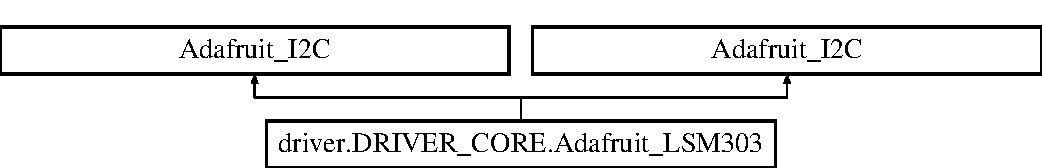
\includegraphics[height=2.000000cm]{classdriver_1_1DRIVER__CORE_1_1Adafruit__LSM303}
\end{center}
\end{figure}
\subsection*{Public Member Functions}
\begin{DoxyCompactItemize}
\item 
\hypertarget{classdriver_1_1DRIVER__CORE_1_1Adafruit__LSM303_ae5cf180d90f8866edaab4807bbe8f7bc}{}def {\bfseries \+\_\+\+\_\+init\+\_\+\+\_\+}\label{classdriver_1_1DRIVER__CORE_1_1Adafruit__LSM303_ae5cf180d90f8866edaab4807bbe8f7bc}

\item 
\hypertarget{classdriver_1_1DRIVER__CORE_1_1Adafruit__LSM303_a73f30f042346b5134d46ac40ea05287c}{}def {\bfseries accel12}\label{classdriver_1_1DRIVER__CORE_1_1Adafruit__LSM303_a73f30f042346b5134d46ac40ea05287c}

\item 
\hypertarget{classdriver_1_1DRIVER__CORE_1_1Adafruit__LSM303_a14da193d80d260f4d95a2636067685ce}{}def {\bfseries mag16}\label{classdriver_1_1DRIVER__CORE_1_1Adafruit__LSM303_a14da193d80d260f4d95a2636067685ce}

\item 
\hypertarget{classdriver_1_1DRIVER__CORE_1_1Adafruit__LSM303_a120ac3815a90e0b4ff49ae60958d568c}{}def {\bfseries read}\label{classdriver_1_1DRIVER__CORE_1_1Adafruit__LSM303_a120ac3815a90e0b4ff49ae60958d568c}

\item 
\hypertarget{classdriver_1_1DRIVER__CORE_1_1Adafruit__LSM303_a91452cc4c7ef0ab07e886843e1cc90dd}{}def {\bfseries set\+Mag\+Gain}\label{classdriver_1_1DRIVER__CORE_1_1Adafruit__LSM303_a91452cc4c7ef0ab07e886843e1cc90dd}

\end{DoxyCompactItemize}
\subsection*{Public Attributes}
\begin{DoxyCompactItemize}
\item 
\hypertarget{classdriver_1_1DRIVER__CORE_1_1Adafruit__LSM303_a17adc9c743af3a5829980b8a702c64d1}{}{\bfseries accel}\label{classdriver_1_1DRIVER__CORE_1_1Adafruit__LSM303_a17adc9c743af3a5829980b8a702c64d1}

\item 
\hypertarget{classdriver_1_1DRIVER__CORE_1_1Adafruit__LSM303_a2afbe1cbd59ce00af91d9e431eb2b391}{}{\bfseries mag}\label{classdriver_1_1DRIVER__CORE_1_1Adafruit__LSM303_a2afbe1cbd59ce00af91d9e431eb2b391}

\end{DoxyCompactItemize}
\subsection*{Static Public Attributes}
\begin{DoxyCompactItemize}
\item 
\hypertarget{classdriver_1_1DRIVER__CORE_1_1Adafruit__LSM303_a24ad319884adc1c09dd29f423b8b6692}{}tuple {\bfseries L\+S\+M303\+\_\+\+A\+D\+D\+R\+E\+S\+S\+\_\+\+A\+C\+C\+E\+L} = (0x32 $>$$>$ 1)\label{classdriver_1_1DRIVER__CORE_1_1Adafruit__LSM303_a24ad319884adc1c09dd29f423b8b6692}

\item 
\hypertarget{classdriver_1_1DRIVER__CORE_1_1Adafruit__LSM303_a0b503ed9efa5d7a4d6edc9e02d1cd61f}{}tuple {\bfseries L\+S\+M303\+\_\+\+A\+D\+D\+R\+E\+S\+S\+\_\+\+M\+A\+G} = (0x3\+C $>$$>$ 1)\label{classdriver_1_1DRIVER__CORE_1_1Adafruit__LSM303_a0b503ed9efa5d7a4d6edc9e02d1cd61f}

\item 
\hypertarget{classdriver_1_1DRIVER__CORE_1_1Adafruit__LSM303_ac907d5dc53fef3f3a59a99e7dd969de2}{}int {\bfseries L\+S\+M303\+\_\+\+R\+E\+G\+I\+S\+T\+E\+R\+\_\+\+A\+C\+C\+E\+L\+\_\+\+C\+T\+R\+L\+\_\+\+R\+E\+G1\+\_\+\+A} = 0x20\label{classdriver_1_1DRIVER__CORE_1_1Adafruit__LSM303_ac907d5dc53fef3f3a59a99e7dd969de2}

\item 
\hypertarget{classdriver_1_1DRIVER__CORE_1_1Adafruit__LSM303_ab9fecee305847de9273f660412fccf01}{}int {\bfseries L\+S\+M303\+\_\+\+R\+E\+G\+I\+S\+T\+E\+R\+\_\+\+A\+C\+C\+E\+L\+\_\+\+C\+T\+R\+L\+\_\+\+R\+E\+G4\+\_\+\+A} = 0x23\label{classdriver_1_1DRIVER__CORE_1_1Adafruit__LSM303_ab9fecee305847de9273f660412fccf01}

\item 
\hypertarget{classdriver_1_1DRIVER__CORE_1_1Adafruit__LSM303_a9db7d714f9448a3ac4121457f1996634}{}int {\bfseries L\+S\+M303\+\_\+\+R\+E\+G\+I\+S\+T\+E\+R\+\_\+\+A\+C\+C\+E\+L\+\_\+\+O\+U\+T\+\_\+\+X\+\_\+\+L\+\_\+\+A} = 0x28\label{classdriver_1_1DRIVER__CORE_1_1Adafruit__LSM303_a9db7d714f9448a3ac4121457f1996634}

\item 
\hypertarget{classdriver_1_1DRIVER__CORE_1_1Adafruit__LSM303_a9ce34b06b2a881fe87f4acf7275e788d}{}int {\bfseries L\+S\+M303\+\_\+\+R\+E\+G\+I\+S\+T\+E\+R\+\_\+\+M\+A\+G\+\_\+\+C\+R\+B\+\_\+\+R\+E\+G\+\_\+\+M} = 0x01\label{classdriver_1_1DRIVER__CORE_1_1Adafruit__LSM303_a9ce34b06b2a881fe87f4acf7275e788d}

\item 
\hypertarget{classdriver_1_1DRIVER__CORE_1_1Adafruit__LSM303_af17a9acb25451a4a2c5f388ff6f95754}{}int {\bfseries L\+S\+M303\+\_\+\+R\+E\+G\+I\+S\+T\+E\+R\+\_\+\+M\+A\+G\+\_\+\+M\+R\+\_\+\+R\+E\+G\+\_\+\+M} = 0x02\label{classdriver_1_1DRIVER__CORE_1_1Adafruit__LSM303_af17a9acb25451a4a2c5f388ff6f95754}

\item 
\hypertarget{classdriver_1_1DRIVER__CORE_1_1Adafruit__LSM303_a39399d95adf47130963ad6228b41f5b5}{}int {\bfseries L\+S\+M303\+\_\+\+R\+E\+G\+I\+S\+T\+E\+R\+\_\+\+M\+A\+G\+\_\+\+O\+U\+T\+\_\+\+X\+\_\+\+H\+\_\+\+M} = 0x03\label{classdriver_1_1DRIVER__CORE_1_1Adafruit__LSM303_a39399d95adf47130963ad6228b41f5b5}

\item 
\hypertarget{classdriver_1_1DRIVER__CORE_1_1Adafruit__LSM303_a7f838baa79a6ae3da80e428f07c0b9ae}{}int {\bfseries L\+S\+M303\+\_\+\+M\+A\+G\+G\+A\+I\+N\+\_\+1\+\_\+3} = 0x20\label{classdriver_1_1DRIVER__CORE_1_1Adafruit__LSM303_a7f838baa79a6ae3da80e428f07c0b9ae}

\item 
\hypertarget{classdriver_1_1DRIVER__CORE_1_1Adafruit__LSM303_a895624eb31381290c41eb4ba15762a21}{}int {\bfseries L\+S\+M303\+\_\+\+M\+A\+G\+G\+A\+I\+N\+\_\+1\+\_\+9} = 0x40\label{classdriver_1_1DRIVER__CORE_1_1Adafruit__LSM303_a895624eb31381290c41eb4ba15762a21}

\item 
\hypertarget{classdriver_1_1DRIVER__CORE_1_1Adafruit__LSM303_a690a2ccf1305ddb8e369e42e140a3d9e}{}int {\bfseries L\+S\+M303\+\_\+\+M\+A\+G\+G\+A\+I\+N\+\_\+2\+\_\+5} = 0x60\label{classdriver_1_1DRIVER__CORE_1_1Adafruit__LSM303_a690a2ccf1305ddb8e369e42e140a3d9e}

\item 
\hypertarget{classdriver_1_1DRIVER__CORE_1_1Adafruit__LSM303_aabf347d0927ecaea47e318cc804e10a0}{}int {\bfseries L\+S\+M303\+\_\+\+M\+A\+G\+G\+A\+I\+N\+\_\+4\+\_\+0} = 0x80\label{classdriver_1_1DRIVER__CORE_1_1Adafruit__LSM303_aabf347d0927ecaea47e318cc804e10a0}

\item 
\hypertarget{classdriver_1_1DRIVER__CORE_1_1Adafruit__LSM303_a1875f919180b6da6408c2d005bb8bdad}{}int {\bfseries L\+S\+M303\+\_\+\+M\+A\+G\+G\+A\+I\+N\+\_\+4\+\_\+7} = 0x\+A0\label{classdriver_1_1DRIVER__CORE_1_1Adafruit__LSM303_a1875f919180b6da6408c2d005bb8bdad}

\item 
\hypertarget{classdriver_1_1DRIVER__CORE_1_1Adafruit__LSM303_a9dfa52c66b43d044d18e642243a4c15d}{}int {\bfseries L\+S\+M303\+\_\+\+M\+A\+G\+G\+A\+I\+N\+\_\+5\+\_\+6} = 0x\+C0\label{classdriver_1_1DRIVER__CORE_1_1Adafruit__LSM303_a9dfa52c66b43d044d18e642243a4c15d}

\item 
\hypertarget{classdriver_1_1DRIVER__CORE_1_1Adafruit__LSM303_a4c33c59d6577266becd976da47b46e7c}{}int {\bfseries L\+S\+M303\+\_\+\+M\+A\+G\+G\+A\+I\+N\+\_\+8\+\_\+1} = 0x\+E0\label{classdriver_1_1DRIVER__CORE_1_1Adafruit__LSM303_a4c33c59d6577266becd976da47b46e7c}

\end{DoxyCompactItemize}


\subsection{Detailed Description}
\begin{DoxyVerb}Python library for Adafruit Flora Accelerometer/Compass Sensor (LSM303).
This is pretty much a direct port of the current Arduino library and is
similarly incomplete (e.g. no orientation value returned from read()
method).  This does add optional high resolution mode to accelerometer
though.

Copyright 2013 Adafruit Industries

Version 0.1

Revised October 10, 2014

Revision Author: Isaac DeSouza (IDS LABS)

Copyright 2014 IDS LABS
\end{DoxyVerb}
 

The documentation for this class was generated from the following file\+:\begin{DoxyCompactItemize}
\item 
D\+R\+I\+V\+E\+R\+\_\+\+C\+O\+R\+E.\+py\end{DoxyCompactItemize}

\hypertarget{classmodel_1_1AstronautModel_1_1AstronautModel}{}\section{model.\+Astronaut\+Model.\+Astronaut\+Model Class Reference}
\label{classmodel_1_1AstronautModel_1_1AstronautModel}\index{model.\+Astronaut\+Model.\+Astronaut\+Model@{model.\+Astronaut\+Model.\+Astronaut\+Model}}
Inheritance diagram for model.\+Astronaut\+Model.\+Astronaut\+Model\+:\begin{figure}[H]
\begin{center}
\leavevmode
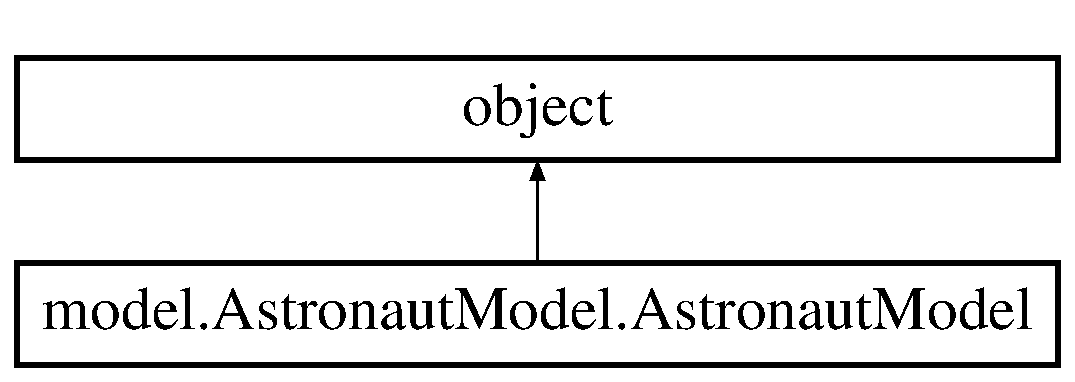
\includegraphics[height=2.000000cm]{classmodel_1_1AstronautModel_1_1AstronautModel}
\end{center}
\end{figure}
\subsection*{Public Member Functions}
\begin{DoxyCompactItemize}
\item 
def \hyperlink{classmodel_1_1AstronautModel_1_1AstronautModel_acf57c389f77b47f834fd3e2959f058d9}{\+\_\+\+\_\+init\+\_\+\+\_\+}
\item 
def \hyperlink{classmodel_1_1AstronautModel_1_1AstronautModel_acf57c389f77b47f834fd3e2959f058d9}{\+\_\+\+\_\+init\+\_\+\+\_\+}
\end{DoxyCompactItemize}
\subsection*{Public Attributes}
\begin{DoxyCompactItemize}
\item 
\hyperlink{classmodel_1_1AstronautModel_1_1AstronautModel_a4f53c5ecfab0292c870d6d8109dacf89}{number}
\item 
\hyperlink{classmodel_1_1AstronautModel_1_1AstronautModel_a396e8b794abeaa7215635523cb03dfb7}{temperature}
\item 
\hyperlink{classmodel_1_1AstronautModel_1_1AstronautModel_a2516ceb31bd5b7af3f4a4d615fad9d11}{power}
\item 
\hyperlink{classmodel_1_1AstronautModel_1_1AstronautModel_a1e054c96ae8431b5f680e7503fe1d72e}{link\+\_\+quality}
\item 
\hyperlink{classmodel_1_1AstronautModel_1_1AstronautModel_a8b5703cbff5b56b1330d1597df28d4f2}{oxygen}
\item 
\hyperlink{classmodel_1_1AstronautModel_1_1AstronautModel_a27568e6a53f8d25875a6f67127e5f25a}{body\+\_\+temperature}
\item 
\hyperlink{classmodel_1_1AstronautModel_1_1AstronautModel_a8bb48117aeee964c627cbdeb7ad89bb5}{heart\+\_\+rate}
\item 
\hyperlink{classmodel_1_1AstronautModel_1_1AstronautModel_a7aca719fe9b712ba6324cf4d337b4ae3}{co2\+\_\+level}
\item 
\hyperlink{classmodel_1_1AstronautModel_1_1AstronautModel_ad1d5c89f4de67fac9f2650edd005e56c}{heading}
\item 
\hyperlink{classmodel_1_1AstronautModel_1_1AstronautModel_a11d42f7b1a897c25839765d6c4c550a3}{waypoint\+\_\+heading}
\item 
\hyperlink{classmodel_1_1AstronautModel_1_1AstronautModel_abf02b7ed56257208a86696d19281568f}{gps}
\item 
\hyperlink{classmodel_1_1AstronautModel_1_1AstronautModel_a84e0cb015b842911625adacccca25047}{distance\+\_\+waypoint}
\item 
\hyperlink{classmodel_1_1AstronautModel_1_1AstronautModel_a852a19df188c9e688ab50fc317fca5d9}{channel\+\_\+listen}
\item 
\hyperlink{classmodel_1_1AstronautModel_1_1AstronautModel_ab727ba1d9681bd7e10dad56fafa33ccd}{channel\+\_\+send}
\end{DoxyCompactItemize}


\subsection{Detailed Description}
\begin{DoxyVerb}docstring for AstronautModel\end{DoxyVerb}
 

\subsection{Constructor \& Destructor Documentation}
\hypertarget{classmodel_1_1AstronautModel_1_1AstronautModel_acf57c389f77b47f834fd3e2959f058d9}{}\index{model\+::\+Astronaut\+Model\+::\+Astronaut\+Model@{model\+::\+Astronaut\+Model\+::\+Astronaut\+Model}!\+\_\+\+\_\+init\+\_\+\+\_\+@{\+\_\+\+\_\+init\+\_\+\+\_\+}}
\index{\+\_\+\+\_\+init\+\_\+\+\_\+@{\+\_\+\+\_\+init\+\_\+\+\_\+}!model\+::\+Astronaut\+Model\+::\+Astronaut\+Model@{model\+::\+Astronaut\+Model\+::\+Astronaut\+Model}}
\subsubsection[{\+\_\+\+\_\+init\+\_\+\+\_\+}]{\setlength{\rightskip}{0pt plus 5cm}def model.\+Astronaut\+Model.\+Astronaut\+Model.\+\_\+\+\_\+init\+\_\+\+\_\+ (
\begin{DoxyParamCaption}
\item[{}]{self, }
\item[{}]{number}
\end{DoxyParamCaption}
)}\label{classmodel_1_1AstronautModel_1_1AstronautModel_acf57c389f77b47f834fd3e2959f058d9}
\hypertarget{classmodel_1_1AstronautModel_1_1AstronautModel_acf57c389f77b47f834fd3e2959f058d9}{}\index{model\+::\+Astronaut\+Model\+::\+Astronaut\+Model@{model\+::\+Astronaut\+Model\+::\+Astronaut\+Model}!\+\_\+\+\_\+init\+\_\+\+\_\+@{\+\_\+\+\_\+init\+\_\+\+\_\+}}
\index{\+\_\+\+\_\+init\+\_\+\+\_\+@{\+\_\+\+\_\+init\+\_\+\+\_\+}!model\+::\+Astronaut\+Model\+::\+Astronaut\+Model@{model\+::\+Astronaut\+Model\+::\+Astronaut\+Model}}
\subsubsection[{\+\_\+\+\_\+init\+\_\+\+\_\+}]{\setlength{\rightskip}{0pt plus 5cm}def model.\+Astronaut\+Model.\+Astronaut\+Model.\+\_\+\+\_\+init\+\_\+\+\_\+ (
\begin{DoxyParamCaption}
\item[{}]{self, }
\item[{}]{number}
\end{DoxyParamCaption}
)}\label{classmodel_1_1AstronautModel_1_1AstronautModel_acf57c389f77b47f834fd3e2959f058d9}


\subsection{Member Data Documentation}
\hypertarget{classmodel_1_1AstronautModel_1_1AstronautModel_a27568e6a53f8d25875a6f67127e5f25a}{}\index{model\+::\+Astronaut\+Model\+::\+Astronaut\+Model@{model\+::\+Astronaut\+Model\+::\+Astronaut\+Model}!body\+\_\+temperature@{body\+\_\+temperature}}
\index{body\+\_\+temperature@{body\+\_\+temperature}!model\+::\+Astronaut\+Model\+::\+Astronaut\+Model@{model\+::\+Astronaut\+Model\+::\+Astronaut\+Model}}
\subsubsection[{body\+\_\+temperature}]{\setlength{\rightskip}{0pt plus 5cm}model.\+Astronaut\+Model.\+Astronaut\+Model.\+body\+\_\+temperature}\label{classmodel_1_1AstronautModel_1_1AstronautModel_a27568e6a53f8d25875a6f67127e5f25a}
\hypertarget{classmodel_1_1AstronautModel_1_1AstronautModel_a852a19df188c9e688ab50fc317fca5d9}{}\index{model\+::\+Astronaut\+Model\+::\+Astronaut\+Model@{model\+::\+Astronaut\+Model\+::\+Astronaut\+Model}!channel\+\_\+listen@{channel\+\_\+listen}}
\index{channel\+\_\+listen@{channel\+\_\+listen}!model\+::\+Astronaut\+Model\+::\+Astronaut\+Model@{model\+::\+Astronaut\+Model\+::\+Astronaut\+Model}}
\subsubsection[{channel\+\_\+listen}]{\setlength{\rightskip}{0pt plus 5cm}model.\+Astronaut\+Model.\+Astronaut\+Model.\+channel\+\_\+listen}\label{classmodel_1_1AstronautModel_1_1AstronautModel_a852a19df188c9e688ab50fc317fca5d9}
\hypertarget{classmodel_1_1AstronautModel_1_1AstronautModel_ab727ba1d9681bd7e10dad56fafa33ccd}{}\index{model\+::\+Astronaut\+Model\+::\+Astronaut\+Model@{model\+::\+Astronaut\+Model\+::\+Astronaut\+Model}!channel\+\_\+send@{channel\+\_\+send}}
\index{channel\+\_\+send@{channel\+\_\+send}!model\+::\+Astronaut\+Model\+::\+Astronaut\+Model@{model\+::\+Astronaut\+Model\+::\+Astronaut\+Model}}
\subsubsection[{channel\+\_\+send}]{\setlength{\rightskip}{0pt plus 5cm}model.\+Astronaut\+Model.\+Astronaut\+Model.\+channel\+\_\+send}\label{classmodel_1_1AstronautModel_1_1AstronautModel_ab727ba1d9681bd7e10dad56fafa33ccd}
\hypertarget{classmodel_1_1AstronautModel_1_1AstronautModel_a7aca719fe9b712ba6324cf4d337b4ae3}{}\index{model\+::\+Astronaut\+Model\+::\+Astronaut\+Model@{model\+::\+Astronaut\+Model\+::\+Astronaut\+Model}!co2\+\_\+level@{co2\+\_\+level}}
\index{co2\+\_\+level@{co2\+\_\+level}!model\+::\+Astronaut\+Model\+::\+Astronaut\+Model@{model\+::\+Astronaut\+Model\+::\+Astronaut\+Model}}
\subsubsection[{co2\+\_\+level}]{\setlength{\rightskip}{0pt plus 5cm}model.\+Astronaut\+Model.\+Astronaut\+Model.\+co2\+\_\+level}\label{classmodel_1_1AstronautModel_1_1AstronautModel_a7aca719fe9b712ba6324cf4d337b4ae3}
\hypertarget{classmodel_1_1AstronautModel_1_1AstronautModel_a84e0cb015b842911625adacccca25047}{}\index{model\+::\+Astronaut\+Model\+::\+Astronaut\+Model@{model\+::\+Astronaut\+Model\+::\+Astronaut\+Model}!distance\+\_\+waypoint@{distance\+\_\+waypoint}}
\index{distance\+\_\+waypoint@{distance\+\_\+waypoint}!model\+::\+Astronaut\+Model\+::\+Astronaut\+Model@{model\+::\+Astronaut\+Model\+::\+Astronaut\+Model}}
\subsubsection[{distance\+\_\+waypoint}]{\setlength{\rightskip}{0pt plus 5cm}model.\+Astronaut\+Model.\+Astronaut\+Model.\+distance\+\_\+waypoint}\label{classmodel_1_1AstronautModel_1_1AstronautModel_a84e0cb015b842911625adacccca25047}
\hypertarget{classmodel_1_1AstronautModel_1_1AstronautModel_abf02b7ed56257208a86696d19281568f}{}\index{model\+::\+Astronaut\+Model\+::\+Astronaut\+Model@{model\+::\+Astronaut\+Model\+::\+Astronaut\+Model}!gps@{gps}}
\index{gps@{gps}!model\+::\+Astronaut\+Model\+::\+Astronaut\+Model@{model\+::\+Astronaut\+Model\+::\+Astronaut\+Model}}
\subsubsection[{gps}]{\setlength{\rightskip}{0pt plus 5cm}model.\+Astronaut\+Model.\+Astronaut\+Model.\+gps}\label{classmodel_1_1AstronautModel_1_1AstronautModel_abf02b7ed56257208a86696d19281568f}
\hypertarget{classmodel_1_1AstronautModel_1_1AstronautModel_ad1d5c89f4de67fac9f2650edd005e56c}{}\index{model\+::\+Astronaut\+Model\+::\+Astronaut\+Model@{model\+::\+Astronaut\+Model\+::\+Astronaut\+Model}!heading@{heading}}
\index{heading@{heading}!model\+::\+Astronaut\+Model\+::\+Astronaut\+Model@{model\+::\+Astronaut\+Model\+::\+Astronaut\+Model}}
\subsubsection[{heading}]{\setlength{\rightskip}{0pt plus 5cm}model.\+Astronaut\+Model.\+Astronaut\+Model.\+heading}\label{classmodel_1_1AstronautModel_1_1AstronautModel_ad1d5c89f4de67fac9f2650edd005e56c}
\hypertarget{classmodel_1_1AstronautModel_1_1AstronautModel_a8bb48117aeee964c627cbdeb7ad89bb5}{}\index{model\+::\+Astronaut\+Model\+::\+Astronaut\+Model@{model\+::\+Astronaut\+Model\+::\+Astronaut\+Model}!heart\+\_\+rate@{heart\+\_\+rate}}
\index{heart\+\_\+rate@{heart\+\_\+rate}!model\+::\+Astronaut\+Model\+::\+Astronaut\+Model@{model\+::\+Astronaut\+Model\+::\+Astronaut\+Model}}
\subsubsection[{heart\+\_\+rate}]{\setlength{\rightskip}{0pt plus 5cm}model.\+Astronaut\+Model.\+Astronaut\+Model.\+heart\+\_\+rate}\label{classmodel_1_1AstronautModel_1_1AstronautModel_a8bb48117aeee964c627cbdeb7ad89bb5}
\hypertarget{classmodel_1_1AstronautModel_1_1AstronautModel_a1e054c96ae8431b5f680e7503fe1d72e}{}\index{model\+::\+Astronaut\+Model\+::\+Astronaut\+Model@{model\+::\+Astronaut\+Model\+::\+Astronaut\+Model}!link\+\_\+quality@{link\+\_\+quality}}
\index{link\+\_\+quality@{link\+\_\+quality}!model\+::\+Astronaut\+Model\+::\+Astronaut\+Model@{model\+::\+Astronaut\+Model\+::\+Astronaut\+Model}}
\subsubsection[{link\+\_\+quality}]{\setlength{\rightskip}{0pt plus 5cm}model.\+Astronaut\+Model.\+Astronaut\+Model.\+link\+\_\+quality}\label{classmodel_1_1AstronautModel_1_1AstronautModel_a1e054c96ae8431b5f680e7503fe1d72e}
\hypertarget{classmodel_1_1AstronautModel_1_1AstronautModel_a4f53c5ecfab0292c870d6d8109dacf89}{}\index{model\+::\+Astronaut\+Model\+::\+Astronaut\+Model@{model\+::\+Astronaut\+Model\+::\+Astronaut\+Model}!number@{number}}
\index{number@{number}!model\+::\+Astronaut\+Model\+::\+Astronaut\+Model@{model\+::\+Astronaut\+Model\+::\+Astronaut\+Model}}
\subsubsection[{number}]{\setlength{\rightskip}{0pt plus 5cm}model.\+Astronaut\+Model.\+Astronaut\+Model.\+number}\label{classmodel_1_1AstronautModel_1_1AstronautModel_a4f53c5ecfab0292c870d6d8109dacf89}
\hypertarget{classmodel_1_1AstronautModel_1_1AstronautModel_a8b5703cbff5b56b1330d1597df28d4f2}{}\index{model\+::\+Astronaut\+Model\+::\+Astronaut\+Model@{model\+::\+Astronaut\+Model\+::\+Astronaut\+Model}!oxygen@{oxygen}}
\index{oxygen@{oxygen}!model\+::\+Astronaut\+Model\+::\+Astronaut\+Model@{model\+::\+Astronaut\+Model\+::\+Astronaut\+Model}}
\subsubsection[{oxygen}]{\setlength{\rightskip}{0pt plus 5cm}model.\+Astronaut\+Model.\+Astronaut\+Model.\+oxygen}\label{classmodel_1_1AstronautModel_1_1AstronautModel_a8b5703cbff5b56b1330d1597df28d4f2}
\hypertarget{classmodel_1_1AstronautModel_1_1AstronautModel_a2516ceb31bd5b7af3f4a4d615fad9d11}{}\index{model\+::\+Astronaut\+Model\+::\+Astronaut\+Model@{model\+::\+Astronaut\+Model\+::\+Astronaut\+Model}!power@{power}}
\index{power@{power}!model\+::\+Astronaut\+Model\+::\+Astronaut\+Model@{model\+::\+Astronaut\+Model\+::\+Astronaut\+Model}}
\subsubsection[{power}]{\setlength{\rightskip}{0pt plus 5cm}model.\+Astronaut\+Model.\+Astronaut\+Model.\+power}\label{classmodel_1_1AstronautModel_1_1AstronautModel_a2516ceb31bd5b7af3f4a4d615fad9d11}
\hypertarget{classmodel_1_1AstronautModel_1_1AstronautModel_a396e8b794abeaa7215635523cb03dfb7}{}\index{model\+::\+Astronaut\+Model\+::\+Astronaut\+Model@{model\+::\+Astronaut\+Model\+::\+Astronaut\+Model}!temperature@{temperature}}
\index{temperature@{temperature}!model\+::\+Astronaut\+Model\+::\+Astronaut\+Model@{model\+::\+Astronaut\+Model\+::\+Astronaut\+Model}}
\subsubsection[{temperature}]{\setlength{\rightskip}{0pt plus 5cm}model.\+Astronaut\+Model.\+Astronaut\+Model.\+temperature}\label{classmodel_1_1AstronautModel_1_1AstronautModel_a396e8b794abeaa7215635523cb03dfb7}
\hypertarget{classmodel_1_1AstronautModel_1_1AstronautModel_a11d42f7b1a897c25839765d6c4c550a3}{}\index{model\+::\+Astronaut\+Model\+::\+Astronaut\+Model@{model\+::\+Astronaut\+Model\+::\+Astronaut\+Model}!waypoint\+\_\+heading@{waypoint\+\_\+heading}}
\index{waypoint\+\_\+heading@{waypoint\+\_\+heading}!model\+::\+Astronaut\+Model\+::\+Astronaut\+Model@{model\+::\+Astronaut\+Model\+::\+Astronaut\+Model}}
\subsubsection[{waypoint\+\_\+heading}]{\setlength{\rightskip}{0pt plus 5cm}model.\+Astronaut\+Model.\+Astronaut\+Model.\+waypoint\+\_\+heading}\label{classmodel_1_1AstronautModel_1_1AstronautModel_a11d42f7b1a897c25839765d6c4c550a3}


The documentation for this class was generated from the following file\+:\begin{DoxyCompactItemize}
\item 
G\+I\+T-\/\+C\+O\+P\+Y/\+Software/model/\hyperlink{GIT-COPY_2Software_2model_2AstronautModel_8py}{Astronaut\+Model.\+py}\end{DoxyCompactItemize}

\hypertarget{classmodel_1_1baseModel_1_1baseModel}{}\section{model.\+base\+Model.\+base\+Model Class Reference}
\label{classmodel_1_1baseModel_1_1baseModel}\index{model.\+base\+Model.\+base\+Model@{model.\+base\+Model.\+base\+Model}}
Inheritance diagram for model.\+base\+Model.\+base\+Model\+:\begin{figure}[H]
\begin{center}
\leavevmode
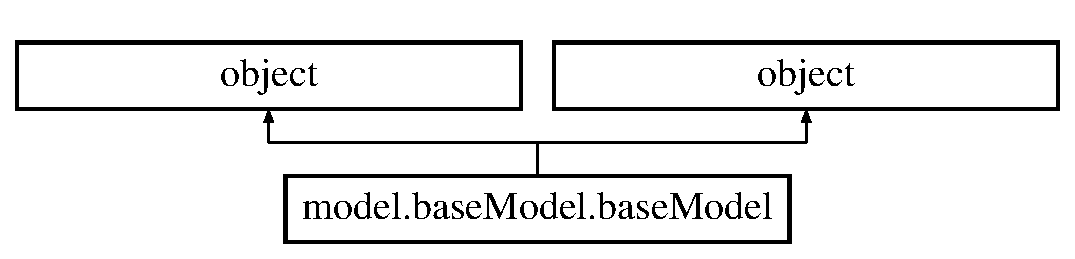
\includegraphics[height=2.000000cm]{classmodel_1_1baseModel_1_1baseModel}
\end{center}
\end{figure}
\subsection*{Public Member Functions}
\begin{DoxyCompactItemize}
\item 
def \hyperlink{classmodel_1_1baseModel_1_1baseModel_ab8d48cf8c0c912c41512fa56fe899744}{\+\_\+\+\_\+init\+\_\+\+\_\+}
\item 
def \hyperlink{classmodel_1_1baseModel_1_1baseModel_ab8d48cf8c0c912c41512fa56fe899744}{\+\_\+\+\_\+init\+\_\+\+\_\+}
\end{DoxyCompactItemize}
\subsection*{Public Attributes}
\begin{DoxyCompactItemize}
\item 
\hyperlink{classmodel_1_1baseModel_1_1baseModel_aaeda64beafa1c2747373d6c4d5a3479f}{name}
\end{DoxyCompactItemize}


\subsection{Constructor \& Destructor Documentation}
\hypertarget{classmodel_1_1baseModel_1_1baseModel_ab8d48cf8c0c912c41512fa56fe899744}{}\index{model\+::base\+Model\+::base\+Model@{model\+::base\+Model\+::base\+Model}!\+\_\+\+\_\+init\+\_\+\+\_\+@{\+\_\+\+\_\+init\+\_\+\+\_\+}}
\index{\+\_\+\+\_\+init\+\_\+\+\_\+@{\+\_\+\+\_\+init\+\_\+\+\_\+}!model\+::base\+Model\+::base\+Model@{model\+::base\+Model\+::base\+Model}}
\subsubsection[{\+\_\+\+\_\+init\+\_\+\+\_\+}]{\setlength{\rightskip}{0pt plus 5cm}def model.\+base\+Model.\+base\+Model.\+\_\+\+\_\+init\+\_\+\+\_\+ (
\begin{DoxyParamCaption}
\item[{}]{self, }
\item[{}]{name}
\end{DoxyParamCaption}
)}\label{classmodel_1_1baseModel_1_1baseModel_ab8d48cf8c0c912c41512fa56fe899744}
\hypertarget{classmodel_1_1baseModel_1_1baseModel_ab8d48cf8c0c912c41512fa56fe899744}{}\index{model\+::base\+Model\+::base\+Model@{model\+::base\+Model\+::base\+Model}!\+\_\+\+\_\+init\+\_\+\+\_\+@{\+\_\+\+\_\+init\+\_\+\+\_\+}}
\index{\+\_\+\+\_\+init\+\_\+\+\_\+@{\+\_\+\+\_\+init\+\_\+\+\_\+}!model\+::base\+Model\+::base\+Model@{model\+::base\+Model\+::base\+Model}}
\subsubsection[{\+\_\+\+\_\+init\+\_\+\+\_\+}]{\setlength{\rightskip}{0pt plus 5cm}def model.\+base\+Model.\+base\+Model.\+\_\+\+\_\+init\+\_\+\+\_\+ (
\begin{DoxyParamCaption}
\item[{}]{self, }
\item[{}]{name}
\end{DoxyParamCaption}
)}\label{classmodel_1_1baseModel_1_1baseModel_ab8d48cf8c0c912c41512fa56fe899744}


\subsection{Member Data Documentation}
\hypertarget{classmodel_1_1baseModel_1_1baseModel_aaeda64beafa1c2747373d6c4d5a3479f}{}\index{model\+::base\+Model\+::base\+Model@{model\+::base\+Model\+::base\+Model}!name@{name}}
\index{name@{name}!model\+::base\+Model\+::base\+Model@{model\+::base\+Model\+::base\+Model}}
\subsubsection[{name}]{\setlength{\rightskip}{0pt plus 5cm}model.\+base\+Model.\+base\+Model.\+name}\label{classmodel_1_1baseModel_1_1baseModel_aaeda64beafa1c2747373d6c4d5a3479f}


The documentation for this class was generated from the following file\+:\begin{DoxyCompactItemize}
\item 
build/lib.\+linux-\/x86\+\_\+64-\/2.\+7/model/\hyperlink{build_2lib_8linux-x86__64-2_87_2model_2baseModel_8py}{base\+Model.\+py}\end{DoxyCompactItemize}

\hypertarget{classnetwork_1_1NETWORK__CORE_1_1CommsThread}{}\section{network.\+N\+E\+T\+W\+O\+R\+K\+\_\+\+C\+O\+R\+E.\+Comms\+Thread Class Reference}
\label{classnetwork_1_1NETWORK__CORE_1_1CommsThread}\index{network.\+N\+E\+T\+W\+O\+R\+K\+\_\+\+C\+O\+R\+E.\+Comms\+Thread@{network.\+N\+E\+T\+W\+O\+R\+K\+\_\+\+C\+O\+R\+E.\+Comms\+Thread}}
Inheritance diagram for network.\+N\+E\+T\+W\+O\+R\+K\+\_\+\+C\+O\+R\+E.\+Comms\+Thread\+:\begin{figure}[H]
\begin{center}
\leavevmode
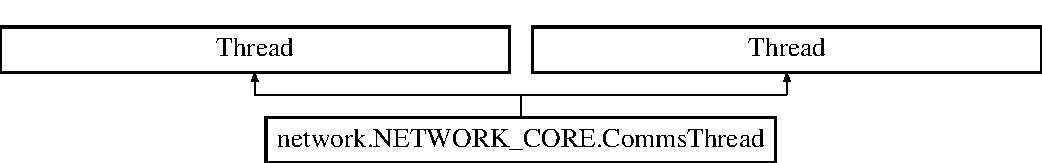
\includegraphics[height=2.000000cm]{classnetwork_1_1NETWORK__CORE_1_1CommsThread}
\end{center}
\end{figure}
\subsection*{Public Member Functions}
\begin{DoxyCompactItemize}
\item 
def \hyperlink{classnetwork_1_1NETWORK__CORE_1_1CommsThread_ab3b9b67bc77d6ed6d5575e97d6031ac6}{\+\_\+\+\_\+init\+\_\+\+\_\+}
\item 
def \hyperlink{classnetwork_1_1NETWORK__CORE_1_1CommsThread_a3d9c7b5081b08434f9c0c70665ebc5f4}{run}
\item 
def \hyperlink{classnetwork_1_1NETWORK__CORE_1_1CommsThread_ab3b9b67bc77d6ed6d5575e97d6031ac6}{\+\_\+\+\_\+init\+\_\+\+\_\+}
\item 
def \hyperlink{classnetwork_1_1NETWORK__CORE_1_1CommsThread_a3d9c7b5081b08434f9c0c70665ebc5f4}{run}
\end{DoxyCompactItemize}
\subsection*{Public Attributes}
\begin{DoxyCompactItemize}
\item 
\hyperlink{classnetwork_1_1NETWORK__CORE_1_1CommsThread_a145170fa3ac9bc02882add7517e0f7fb}{is\+Running}
\item 
\hyperlink{classnetwork_1_1NETWORK__CORE_1_1CommsThread_ad9629d20873b3079e6dc087f6fab8991}{num}
\item 
\hyperlink{classnetwork_1_1NETWORK__CORE_1_1CommsThread_a266630b3cfcdac365332bab1b70cd811}{funct}
\item 
\hyperlink{classnetwork_1_1NETWORK__CORE_1_1CommsThread_ab1cf0c0ed573a7a2f840f82be860a3a9}{arg}
\end{DoxyCompactItemize}


\subsection{Constructor \& Destructor Documentation}
\hypertarget{classnetwork_1_1NETWORK__CORE_1_1CommsThread_ab3b9b67bc77d6ed6d5575e97d6031ac6}{}\index{network\+::\+N\+E\+T\+W\+O\+R\+K\+\_\+\+C\+O\+R\+E\+::\+Comms\+Thread@{network\+::\+N\+E\+T\+W\+O\+R\+K\+\_\+\+C\+O\+R\+E\+::\+Comms\+Thread}!\+\_\+\+\_\+init\+\_\+\+\_\+@{\+\_\+\+\_\+init\+\_\+\+\_\+}}
\index{\+\_\+\+\_\+init\+\_\+\+\_\+@{\+\_\+\+\_\+init\+\_\+\+\_\+}!network\+::\+N\+E\+T\+W\+O\+R\+K\+\_\+\+C\+O\+R\+E\+::\+Comms\+Thread@{network\+::\+N\+E\+T\+W\+O\+R\+K\+\_\+\+C\+O\+R\+E\+::\+Comms\+Thread}}
\subsubsection[{\+\_\+\+\_\+init\+\_\+\+\_\+}]{\setlength{\rightskip}{0pt plus 5cm}def network.\+N\+E\+T\+W\+O\+R\+K\+\_\+\+C\+O\+R\+E.\+Comms\+Thread.\+\_\+\+\_\+init\+\_\+\+\_\+ (
\begin{DoxyParamCaption}
\item[{}]{self, }
\item[{}]{num, }
\item[{}]{funct, }
\item[{}]{arg = {\ttfamily None}}
\end{DoxyParamCaption}
)}\label{classnetwork_1_1NETWORK__CORE_1_1CommsThread_ab3b9b67bc77d6ed6d5575e97d6031ac6}
\hypertarget{classnetwork_1_1NETWORK__CORE_1_1CommsThread_ab3b9b67bc77d6ed6d5575e97d6031ac6}{}\index{network\+::\+N\+E\+T\+W\+O\+R\+K\+\_\+\+C\+O\+R\+E\+::\+Comms\+Thread@{network\+::\+N\+E\+T\+W\+O\+R\+K\+\_\+\+C\+O\+R\+E\+::\+Comms\+Thread}!\+\_\+\+\_\+init\+\_\+\+\_\+@{\+\_\+\+\_\+init\+\_\+\+\_\+}}
\index{\+\_\+\+\_\+init\+\_\+\+\_\+@{\+\_\+\+\_\+init\+\_\+\+\_\+}!network\+::\+N\+E\+T\+W\+O\+R\+K\+\_\+\+C\+O\+R\+E\+::\+Comms\+Thread@{network\+::\+N\+E\+T\+W\+O\+R\+K\+\_\+\+C\+O\+R\+E\+::\+Comms\+Thread}}
\subsubsection[{\+\_\+\+\_\+init\+\_\+\+\_\+}]{\setlength{\rightskip}{0pt plus 5cm}def network.\+N\+E\+T\+W\+O\+R\+K\+\_\+\+C\+O\+R\+E.\+Comms\+Thread.\+\_\+\+\_\+init\+\_\+\+\_\+ (
\begin{DoxyParamCaption}
\item[{}]{self, }
\item[{}]{num, }
\item[{}]{funct, }
\item[{}]{arg = {\ttfamily None}}
\end{DoxyParamCaption}
)}\label{classnetwork_1_1NETWORK__CORE_1_1CommsThread_ab3b9b67bc77d6ed6d5575e97d6031ac6}


\subsection{Member Function Documentation}
\hypertarget{classnetwork_1_1NETWORK__CORE_1_1CommsThread_a3d9c7b5081b08434f9c0c70665ebc5f4}{}\index{network\+::\+N\+E\+T\+W\+O\+R\+K\+\_\+\+C\+O\+R\+E\+::\+Comms\+Thread@{network\+::\+N\+E\+T\+W\+O\+R\+K\+\_\+\+C\+O\+R\+E\+::\+Comms\+Thread}!run@{run}}
\index{run@{run}!network\+::\+N\+E\+T\+W\+O\+R\+K\+\_\+\+C\+O\+R\+E\+::\+Comms\+Thread@{network\+::\+N\+E\+T\+W\+O\+R\+K\+\_\+\+C\+O\+R\+E\+::\+Comms\+Thread}}
\subsubsection[{run}]{\setlength{\rightskip}{0pt plus 5cm}def network.\+N\+E\+T\+W\+O\+R\+K\+\_\+\+C\+O\+R\+E.\+Comms\+Thread.\+run (
\begin{DoxyParamCaption}
\item[{}]{self}
\end{DoxyParamCaption}
)}\label{classnetwork_1_1NETWORK__CORE_1_1CommsThread_a3d9c7b5081b08434f9c0c70665ebc5f4}
\hypertarget{classnetwork_1_1NETWORK__CORE_1_1CommsThread_a3d9c7b5081b08434f9c0c70665ebc5f4}{}\index{network\+::\+N\+E\+T\+W\+O\+R\+K\+\_\+\+C\+O\+R\+E\+::\+Comms\+Thread@{network\+::\+N\+E\+T\+W\+O\+R\+K\+\_\+\+C\+O\+R\+E\+::\+Comms\+Thread}!run@{run}}
\index{run@{run}!network\+::\+N\+E\+T\+W\+O\+R\+K\+\_\+\+C\+O\+R\+E\+::\+Comms\+Thread@{network\+::\+N\+E\+T\+W\+O\+R\+K\+\_\+\+C\+O\+R\+E\+::\+Comms\+Thread}}
\subsubsection[{run}]{\setlength{\rightskip}{0pt plus 5cm}def network.\+N\+E\+T\+W\+O\+R\+K\+\_\+\+C\+O\+R\+E.\+Comms\+Thread.\+run (
\begin{DoxyParamCaption}
\item[{}]{self}
\end{DoxyParamCaption}
)}\label{classnetwork_1_1NETWORK__CORE_1_1CommsThread_a3d9c7b5081b08434f9c0c70665ebc5f4}


\subsection{Member Data Documentation}
\hypertarget{classnetwork_1_1NETWORK__CORE_1_1CommsThread_ab1cf0c0ed573a7a2f840f82be860a3a9}{}\index{network\+::\+N\+E\+T\+W\+O\+R\+K\+\_\+\+C\+O\+R\+E\+::\+Comms\+Thread@{network\+::\+N\+E\+T\+W\+O\+R\+K\+\_\+\+C\+O\+R\+E\+::\+Comms\+Thread}!arg@{arg}}
\index{arg@{arg}!network\+::\+N\+E\+T\+W\+O\+R\+K\+\_\+\+C\+O\+R\+E\+::\+Comms\+Thread@{network\+::\+N\+E\+T\+W\+O\+R\+K\+\_\+\+C\+O\+R\+E\+::\+Comms\+Thread}}
\subsubsection[{arg}]{\setlength{\rightskip}{0pt plus 5cm}network.\+N\+E\+T\+W\+O\+R\+K\+\_\+\+C\+O\+R\+E.\+Comms\+Thread.\+arg}\label{classnetwork_1_1NETWORK__CORE_1_1CommsThread_ab1cf0c0ed573a7a2f840f82be860a3a9}
\hypertarget{classnetwork_1_1NETWORK__CORE_1_1CommsThread_a266630b3cfcdac365332bab1b70cd811}{}\index{network\+::\+N\+E\+T\+W\+O\+R\+K\+\_\+\+C\+O\+R\+E\+::\+Comms\+Thread@{network\+::\+N\+E\+T\+W\+O\+R\+K\+\_\+\+C\+O\+R\+E\+::\+Comms\+Thread}!funct@{funct}}
\index{funct@{funct}!network\+::\+N\+E\+T\+W\+O\+R\+K\+\_\+\+C\+O\+R\+E\+::\+Comms\+Thread@{network\+::\+N\+E\+T\+W\+O\+R\+K\+\_\+\+C\+O\+R\+E\+::\+Comms\+Thread}}
\subsubsection[{funct}]{\setlength{\rightskip}{0pt plus 5cm}network.\+N\+E\+T\+W\+O\+R\+K\+\_\+\+C\+O\+R\+E.\+Comms\+Thread.\+funct}\label{classnetwork_1_1NETWORK__CORE_1_1CommsThread_a266630b3cfcdac365332bab1b70cd811}
\hypertarget{classnetwork_1_1NETWORK__CORE_1_1CommsThread_a145170fa3ac9bc02882add7517e0f7fb}{}\index{network\+::\+N\+E\+T\+W\+O\+R\+K\+\_\+\+C\+O\+R\+E\+::\+Comms\+Thread@{network\+::\+N\+E\+T\+W\+O\+R\+K\+\_\+\+C\+O\+R\+E\+::\+Comms\+Thread}!is\+Running@{is\+Running}}
\index{is\+Running@{is\+Running}!network\+::\+N\+E\+T\+W\+O\+R\+K\+\_\+\+C\+O\+R\+E\+::\+Comms\+Thread@{network\+::\+N\+E\+T\+W\+O\+R\+K\+\_\+\+C\+O\+R\+E\+::\+Comms\+Thread}}
\subsubsection[{is\+Running}]{\setlength{\rightskip}{0pt plus 5cm}network.\+N\+E\+T\+W\+O\+R\+K\+\_\+\+C\+O\+R\+E.\+Comms\+Thread.\+is\+Running}\label{classnetwork_1_1NETWORK__CORE_1_1CommsThread_a145170fa3ac9bc02882add7517e0f7fb}
\hypertarget{classnetwork_1_1NETWORK__CORE_1_1CommsThread_ad9629d20873b3079e6dc087f6fab8991}{}\index{network\+::\+N\+E\+T\+W\+O\+R\+K\+\_\+\+C\+O\+R\+E\+::\+Comms\+Thread@{network\+::\+N\+E\+T\+W\+O\+R\+K\+\_\+\+C\+O\+R\+E\+::\+Comms\+Thread}!num@{num}}
\index{num@{num}!network\+::\+N\+E\+T\+W\+O\+R\+K\+\_\+\+C\+O\+R\+E\+::\+Comms\+Thread@{network\+::\+N\+E\+T\+W\+O\+R\+K\+\_\+\+C\+O\+R\+E\+::\+Comms\+Thread}}
\subsubsection[{num}]{\setlength{\rightskip}{0pt plus 5cm}network.\+N\+E\+T\+W\+O\+R\+K\+\_\+\+C\+O\+R\+E.\+Comms\+Thread.\+num}\label{classnetwork_1_1NETWORK__CORE_1_1CommsThread_ad9629d20873b3079e6dc087f6fab8991}


The documentation for this class was generated from the following file\+:\begin{DoxyCompactItemize}
\item 
build/lib.\+linux-\/x86\+\_\+64-\/2.\+7/network/\hyperlink{build_2lib_8linux-x86__64-2_87_2network_2NETWORK__CORE_8py}{N\+E\+T\+W\+O\+R\+K\+\_\+\+C\+O\+R\+E.\+py}\end{DoxyCompactItemize}

\hypertarget{classnetwork_1_1commsChannel_1_1CommsThread}{}\section{network.\+comms\+Channel.\+Comms\+Thread Class Reference}
\label{classnetwork_1_1commsChannel_1_1CommsThread}\index{network.\+comms\+Channel.\+Comms\+Thread@{network.\+comms\+Channel.\+Comms\+Thread}}
Inheritance diagram for network.\+comms\+Channel.\+Comms\+Thread\+:\begin{figure}[H]
\begin{center}
\leavevmode
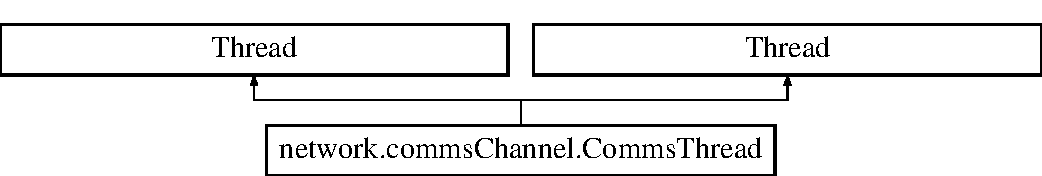
\includegraphics[height=2.000000cm]{classnetwork_1_1commsChannel_1_1CommsThread}
\end{center}
\end{figure}
\subsection*{Public Member Functions}
\begin{DoxyCompactItemize}
\item 
def \hyperlink{classnetwork_1_1commsChannel_1_1CommsThread_a1a23f3e9d80d65392dc9c2710c95443a}{\+\_\+\+\_\+init\+\_\+\+\_\+}
\item 
def \hyperlink{classnetwork_1_1commsChannel_1_1CommsThread_a80d7c1196d9c22fa9b5c892187f0fda9}{run}
\item 
def \hyperlink{classnetwork_1_1commsChannel_1_1CommsThread_a1a23f3e9d80d65392dc9c2710c95443a}{\+\_\+\+\_\+init\+\_\+\+\_\+}
\item 
def \hyperlink{classnetwork_1_1commsChannel_1_1CommsThread_a80d7c1196d9c22fa9b5c892187f0fda9}{run}
\end{DoxyCompactItemize}
\subsection*{Public Attributes}
\begin{DoxyCompactItemize}
\item 
\hyperlink{classnetwork_1_1commsChannel_1_1CommsThread_a19b489cfef0f927e73c891f06f971745}{is\+Running}
\item 
\hyperlink{classnetwork_1_1commsChannel_1_1CommsThread_a2201049bdb76e1bff371c2ef1446eeb6}{num}
\item 
\hyperlink{classnetwork_1_1commsChannel_1_1CommsThread_a84740c23a68c30c4ae6596cb4a023661}{funct}
\item 
\hyperlink{classnetwork_1_1commsChannel_1_1CommsThread_aca064a0602473a73a38ba33d335ebfd2}{arg}
\end{DoxyCompactItemize}


\subsection{Constructor \& Destructor Documentation}
\hypertarget{classnetwork_1_1commsChannel_1_1CommsThread_a1a23f3e9d80d65392dc9c2710c95443a}{}\index{network\+::comms\+Channel\+::\+Comms\+Thread@{network\+::comms\+Channel\+::\+Comms\+Thread}!\+\_\+\+\_\+init\+\_\+\+\_\+@{\+\_\+\+\_\+init\+\_\+\+\_\+}}
\index{\+\_\+\+\_\+init\+\_\+\+\_\+@{\+\_\+\+\_\+init\+\_\+\+\_\+}!network\+::comms\+Channel\+::\+Comms\+Thread@{network\+::comms\+Channel\+::\+Comms\+Thread}}
\subsubsection[{\+\_\+\+\_\+init\+\_\+\+\_\+}]{\setlength{\rightskip}{0pt plus 5cm}def network.\+comms\+Channel.\+Comms\+Thread.\+\_\+\+\_\+init\+\_\+\+\_\+ (
\begin{DoxyParamCaption}
\item[{}]{self, }
\item[{}]{num, }
\item[{}]{funct, }
\item[{}]{arg = {\ttfamily None}}
\end{DoxyParamCaption}
)}\label{classnetwork_1_1commsChannel_1_1CommsThread_a1a23f3e9d80d65392dc9c2710c95443a}
\hypertarget{classnetwork_1_1commsChannel_1_1CommsThread_a1a23f3e9d80d65392dc9c2710c95443a}{}\index{network\+::comms\+Channel\+::\+Comms\+Thread@{network\+::comms\+Channel\+::\+Comms\+Thread}!\+\_\+\+\_\+init\+\_\+\+\_\+@{\+\_\+\+\_\+init\+\_\+\+\_\+}}
\index{\+\_\+\+\_\+init\+\_\+\+\_\+@{\+\_\+\+\_\+init\+\_\+\+\_\+}!network\+::comms\+Channel\+::\+Comms\+Thread@{network\+::comms\+Channel\+::\+Comms\+Thread}}
\subsubsection[{\+\_\+\+\_\+init\+\_\+\+\_\+}]{\setlength{\rightskip}{0pt plus 5cm}def network.\+comms\+Channel.\+Comms\+Thread.\+\_\+\+\_\+init\+\_\+\+\_\+ (
\begin{DoxyParamCaption}
\item[{}]{self, }
\item[{}]{num, }
\item[{}]{funct, }
\item[{}]{arg = {\ttfamily None}}
\end{DoxyParamCaption}
)}\label{classnetwork_1_1commsChannel_1_1CommsThread_a1a23f3e9d80d65392dc9c2710c95443a}


\subsection{Member Function Documentation}
\hypertarget{classnetwork_1_1commsChannel_1_1CommsThread_a80d7c1196d9c22fa9b5c892187f0fda9}{}\index{network\+::comms\+Channel\+::\+Comms\+Thread@{network\+::comms\+Channel\+::\+Comms\+Thread}!run@{run}}
\index{run@{run}!network\+::comms\+Channel\+::\+Comms\+Thread@{network\+::comms\+Channel\+::\+Comms\+Thread}}
\subsubsection[{run}]{\setlength{\rightskip}{0pt plus 5cm}def network.\+comms\+Channel.\+Comms\+Thread.\+run (
\begin{DoxyParamCaption}
\item[{}]{self}
\end{DoxyParamCaption}
)}\label{classnetwork_1_1commsChannel_1_1CommsThread_a80d7c1196d9c22fa9b5c892187f0fda9}
\hypertarget{classnetwork_1_1commsChannel_1_1CommsThread_a80d7c1196d9c22fa9b5c892187f0fda9}{}\index{network\+::comms\+Channel\+::\+Comms\+Thread@{network\+::comms\+Channel\+::\+Comms\+Thread}!run@{run}}
\index{run@{run}!network\+::comms\+Channel\+::\+Comms\+Thread@{network\+::comms\+Channel\+::\+Comms\+Thread}}
\subsubsection[{run}]{\setlength{\rightskip}{0pt plus 5cm}def network.\+comms\+Channel.\+Comms\+Thread.\+run (
\begin{DoxyParamCaption}
\item[{}]{self}
\end{DoxyParamCaption}
)}\label{classnetwork_1_1commsChannel_1_1CommsThread_a80d7c1196d9c22fa9b5c892187f0fda9}


\subsection{Member Data Documentation}
\hypertarget{classnetwork_1_1commsChannel_1_1CommsThread_aca064a0602473a73a38ba33d335ebfd2}{}\index{network\+::comms\+Channel\+::\+Comms\+Thread@{network\+::comms\+Channel\+::\+Comms\+Thread}!arg@{arg}}
\index{arg@{arg}!network\+::comms\+Channel\+::\+Comms\+Thread@{network\+::comms\+Channel\+::\+Comms\+Thread}}
\subsubsection[{arg}]{\setlength{\rightskip}{0pt plus 5cm}network.\+comms\+Channel.\+Comms\+Thread.\+arg}\label{classnetwork_1_1commsChannel_1_1CommsThread_aca064a0602473a73a38ba33d335ebfd2}
\hypertarget{classnetwork_1_1commsChannel_1_1CommsThread_a84740c23a68c30c4ae6596cb4a023661}{}\index{network\+::comms\+Channel\+::\+Comms\+Thread@{network\+::comms\+Channel\+::\+Comms\+Thread}!funct@{funct}}
\index{funct@{funct}!network\+::comms\+Channel\+::\+Comms\+Thread@{network\+::comms\+Channel\+::\+Comms\+Thread}}
\subsubsection[{funct}]{\setlength{\rightskip}{0pt plus 5cm}network.\+comms\+Channel.\+Comms\+Thread.\+funct}\label{classnetwork_1_1commsChannel_1_1CommsThread_a84740c23a68c30c4ae6596cb4a023661}
\hypertarget{classnetwork_1_1commsChannel_1_1CommsThread_a19b489cfef0f927e73c891f06f971745}{}\index{network\+::comms\+Channel\+::\+Comms\+Thread@{network\+::comms\+Channel\+::\+Comms\+Thread}!is\+Running@{is\+Running}}
\index{is\+Running@{is\+Running}!network\+::comms\+Channel\+::\+Comms\+Thread@{network\+::comms\+Channel\+::\+Comms\+Thread}}
\subsubsection[{is\+Running}]{\setlength{\rightskip}{0pt plus 5cm}network.\+comms\+Channel.\+Comms\+Thread.\+is\+Running}\label{classnetwork_1_1commsChannel_1_1CommsThread_a19b489cfef0f927e73c891f06f971745}
\hypertarget{classnetwork_1_1commsChannel_1_1CommsThread_a2201049bdb76e1bff371c2ef1446eeb6}{}\index{network\+::comms\+Channel\+::\+Comms\+Thread@{network\+::comms\+Channel\+::\+Comms\+Thread}!num@{num}}
\index{num@{num}!network\+::comms\+Channel\+::\+Comms\+Thread@{network\+::comms\+Channel\+::\+Comms\+Thread}}
\subsubsection[{num}]{\setlength{\rightskip}{0pt plus 5cm}network.\+comms\+Channel.\+Comms\+Thread.\+num}\label{classnetwork_1_1commsChannel_1_1CommsThread_a2201049bdb76e1bff371c2ef1446eeb6}


The documentation for this class was generated from the following file\+:\begin{DoxyCompactItemize}
\item 
build/lib.\+linux-\/x86\+\_\+64-\/2.\+7/network/\hyperlink{build_2lib_8linux-x86__64-2_87_2network_2commsChannel_8py}{comms\+Channel.\+py}\end{DoxyCompactItemize}

\hypertarget{classcontroller_1_1controller_1_1Controller}{}\section{controller.\+controller.\+Controller Class Reference}
\label{classcontroller_1_1controller_1_1Controller}\index{controller.\+controller.\+Controller@{controller.\+controller.\+Controller}}
Inheritance diagram for controller.\+controller.\+Controller\+:\begin{figure}[H]
\begin{center}
\leavevmode
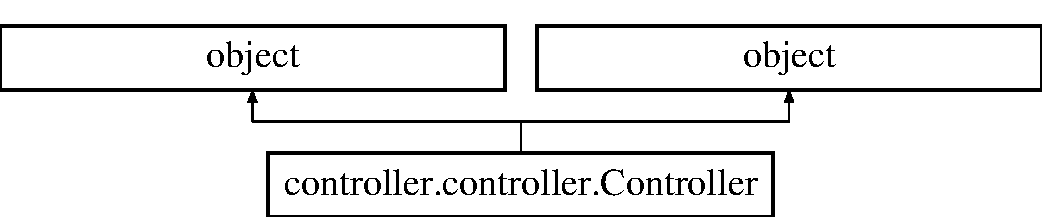
\includegraphics[height=2.000000cm]{classcontroller_1_1controller_1_1Controller}
\end{center}
\end{figure}
\subsection*{Public Member Functions}
\begin{DoxyCompactItemize}
\item 
def \hyperlink{classcontroller_1_1controller_1_1Controller_a3d1afce0394fdd46f748161ac6078bd1}{\+\_\+\+\_\+init\+\_\+\+\_\+}
\item 
def \hyperlink{classcontroller_1_1controller_1_1Controller_a5302cdeab4a3beda9c476188bad72023}{add\+Channel}
\item 
def \hyperlink{classcontroller_1_1controller_1_1Controller_a3d1afce0394fdd46f748161ac6078bd1}{\+\_\+\+\_\+init\+\_\+\+\_\+}
\item 
def \hyperlink{classcontroller_1_1controller_1_1Controller_a5302cdeab4a3beda9c476188bad72023}{add\+Channel}
\end{DoxyCompactItemize}
\subsection*{Public Attributes}
\begin{DoxyCompactItemize}
\item 
\hyperlink{classcontroller_1_1controller_1_1Controller_a954001a416c1af88b29758ccede576c1}{channels}
\end{DoxyCompactItemize}


\subsection{Constructor \& Destructor Documentation}
\hypertarget{classcontroller_1_1controller_1_1Controller_a3d1afce0394fdd46f748161ac6078bd1}{}\index{controller\+::controller\+::\+Controller@{controller\+::controller\+::\+Controller}!\+\_\+\+\_\+init\+\_\+\+\_\+@{\+\_\+\+\_\+init\+\_\+\+\_\+}}
\index{\+\_\+\+\_\+init\+\_\+\+\_\+@{\+\_\+\+\_\+init\+\_\+\+\_\+}!controller\+::controller\+::\+Controller@{controller\+::controller\+::\+Controller}}
\subsubsection[{\+\_\+\+\_\+init\+\_\+\+\_\+}]{\setlength{\rightskip}{0pt plus 5cm}def controller.\+controller.\+Controller.\+\_\+\+\_\+init\+\_\+\+\_\+ (
\begin{DoxyParamCaption}
\item[{}]{self}
\end{DoxyParamCaption}
)}\label{classcontroller_1_1controller_1_1Controller_a3d1afce0394fdd46f748161ac6078bd1}
\hypertarget{classcontroller_1_1controller_1_1Controller_a3d1afce0394fdd46f748161ac6078bd1}{}\index{controller\+::controller\+::\+Controller@{controller\+::controller\+::\+Controller}!\+\_\+\+\_\+init\+\_\+\+\_\+@{\+\_\+\+\_\+init\+\_\+\+\_\+}}
\index{\+\_\+\+\_\+init\+\_\+\+\_\+@{\+\_\+\+\_\+init\+\_\+\+\_\+}!controller\+::controller\+::\+Controller@{controller\+::controller\+::\+Controller}}
\subsubsection[{\+\_\+\+\_\+init\+\_\+\+\_\+}]{\setlength{\rightskip}{0pt plus 5cm}def controller.\+controller.\+Controller.\+\_\+\+\_\+init\+\_\+\+\_\+ (
\begin{DoxyParamCaption}
\item[{}]{self}
\end{DoxyParamCaption}
)}\label{classcontroller_1_1controller_1_1Controller_a3d1afce0394fdd46f748161ac6078bd1}


\subsection{Member Function Documentation}
\hypertarget{classcontroller_1_1controller_1_1Controller_a5302cdeab4a3beda9c476188bad72023}{}\index{controller\+::controller\+::\+Controller@{controller\+::controller\+::\+Controller}!add\+Channel@{add\+Channel}}
\index{add\+Channel@{add\+Channel}!controller\+::controller\+::\+Controller@{controller\+::controller\+::\+Controller}}
\subsubsection[{add\+Channel}]{\setlength{\rightskip}{0pt plus 5cm}def controller.\+controller.\+Controller.\+add\+Channel (
\begin{DoxyParamCaption}
\item[{}]{self, }
\item[{}]{channel, }
\item[{}]{recv\+Funct}
\end{DoxyParamCaption}
)}\label{classcontroller_1_1controller_1_1Controller_a5302cdeab4a3beda9c476188bad72023}
\hypertarget{classcontroller_1_1controller_1_1Controller_a5302cdeab4a3beda9c476188bad72023}{}\index{controller\+::controller\+::\+Controller@{controller\+::controller\+::\+Controller}!add\+Channel@{add\+Channel}}
\index{add\+Channel@{add\+Channel}!controller\+::controller\+::\+Controller@{controller\+::controller\+::\+Controller}}
\subsubsection[{add\+Channel}]{\setlength{\rightskip}{0pt plus 5cm}def controller.\+controller.\+Controller.\+add\+Channel (
\begin{DoxyParamCaption}
\item[{}]{self, }
\item[{}]{channel, }
\item[{}]{recv\+Funct}
\end{DoxyParamCaption}
)}\label{classcontroller_1_1controller_1_1Controller_a5302cdeab4a3beda9c476188bad72023}


\subsection{Member Data Documentation}
\hypertarget{classcontroller_1_1controller_1_1Controller_a954001a416c1af88b29758ccede576c1}{}\index{controller\+::controller\+::\+Controller@{controller\+::controller\+::\+Controller}!channels@{channels}}
\index{channels@{channels}!controller\+::controller\+::\+Controller@{controller\+::controller\+::\+Controller}}
\subsubsection[{channels}]{\setlength{\rightskip}{0pt plus 5cm}controller.\+controller.\+Controller.\+channels}\label{classcontroller_1_1controller_1_1Controller_a954001a416c1af88b29758ccede576c1}


The documentation for this class was generated from the following file\+:\begin{DoxyCompactItemize}
\item 
build/lib.\+linux-\/x86\+\_\+64-\/2.\+7/controller/\hyperlink{build_2lib_8linux-x86__64-2_87_2controller_2controller_8py}{controller.\+py}\end{DoxyCompactItemize}

\hypertarget{classinterface_1_1MOTOR__CORE_1_1DC}{}\section{interface.\+M\+O\+T\+O\+R\+\_\+\+C\+O\+R\+E.\+D\+C Class Reference}
\label{classinterface_1_1MOTOR__CORE_1_1DC}\index{interface.\+M\+O\+T\+O\+R\+\_\+\+C\+O\+R\+E.\+D\+C@{interface.\+M\+O\+T\+O\+R\+\_\+\+C\+O\+R\+E.\+D\+C}}


This class defines types of supported motor drivers and methods to use them.  


\subsection*{Public Member Functions}
\begin{DoxyCompactItemize}
\item 
def \hyperlink{classinterface_1_1MOTOR__CORE_1_1DC_a7adcb2ca9d22b0a94b53a09347f9c2b7}{\+\_\+\+\_\+init\+\_\+\+\_\+}
\item 
def \hyperlink{classinterface_1_1MOTOR__CORE_1_1DC_a07432431affa760aec0760871db95d59}{set\+Pololu\+V\+N\+H5019}
\begin{DoxyCompactList}\small\item\em This motor driver requires 3 pins for control. \end{DoxyCompactList}\item 
def \hyperlink{classinterface_1_1MOTOR__CORE_1_1DC_a562d14585f151182842fe34106a1d88c}{set\+Pololu\+H\+P\+D}
\begin{DoxyCompactList}\small\item\em This motor driver requires 3 pins for control. \end{DoxyCompactList}\item 
def \hyperlink{classinterface_1_1MOTOR__CORE_1_1DC_a11b3993f834e3a032134faacc590ad6a}{set\+Up\+Servo}
\begin{DoxyCompactList}\small\item\em This connects to the servo directly to the P\+C\+A9865 driver. \end{DoxyCompactList}\item 
def \hyperlink{classinterface_1_1MOTOR__CORE_1_1DC_acd058e10f316149548b64f26a75f6dc5}{set\+Motor\+Power}
\begin{DoxyCompactList}\small\item\em Sets the power from 0 to 100 \% for motor defined. \end{DoxyCompactList}\item 
def \hyperlink{classinterface_1_1MOTOR__CORE_1_1DC_a9d0cb15bc32abd7e5ffef57a9d83c9b1}{set\+Servo\+Power}
\begin{DoxyCompactList}\small\item\em Set the pulse width for the servo. \end{DoxyCompactList}\item 
def \hyperlink{classinterface_1_1MOTOR__CORE_1_1DC_a143580f4f51c92080dd75f2b70b56d2d}{\+\_\+\+\_\+send\+Command\+\_\+\+\_\+}
\item 
def \hyperlink{classinterface_1_1MOTOR__CORE_1_1DC_a7adcb2ca9d22b0a94b53a09347f9c2b7}{\+\_\+\+\_\+init\+\_\+\+\_\+}
\item 
def \hyperlink{classinterface_1_1MOTOR__CORE_1_1DC_a07432431affa760aec0760871db95d59}{set\+Pololu\+V\+N\+H5019}
\begin{DoxyCompactList}\small\item\em This motor driver requires 3 pins for control. \end{DoxyCompactList}\item 
def \hyperlink{classinterface_1_1MOTOR__CORE_1_1DC_a562d14585f151182842fe34106a1d88c}{set\+Pololu\+H\+P\+D}
\begin{DoxyCompactList}\small\item\em This motor driver requires 3 pins for control. \end{DoxyCompactList}\item 
def \hyperlink{classinterface_1_1MOTOR__CORE_1_1DC_a11b3993f834e3a032134faacc590ad6a}{set\+Up\+Servo}
\begin{DoxyCompactList}\small\item\em This connects to the servo directly to the P\+C\+A9865 driver. \end{DoxyCompactList}\item 
def \hyperlink{classinterface_1_1MOTOR__CORE_1_1DC_acd058e10f316149548b64f26a75f6dc5}{set\+Motor\+Power}
\begin{DoxyCompactList}\small\item\em Sets the power from 0 to 100 \% for motor defined. \end{DoxyCompactList}\item 
def \hyperlink{classinterface_1_1MOTOR__CORE_1_1DC_a9d0cb15bc32abd7e5ffef57a9d83c9b1}{set\+Servo\+Power}
\begin{DoxyCompactList}\small\item\em Set the pulse width for the servo. \end{DoxyCompactList}\item 
def \hyperlink{classinterface_1_1MOTOR__CORE_1_1DC_a143580f4f51c92080dd75f2b70b56d2d}{\+\_\+\+\_\+send\+Command\+\_\+\+\_\+}
\item 
def \hyperlink{classinterface_1_1MOTOR__CORE_1_1DC_a7adcb2ca9d22b0a94b53a09347f9c2b7}{\+\_\+\+\_\+init\+\_\+\+\_\+}
\item 
def \hyperlink{classinterface_1_1MOTOR__CORE_1_1DC_a07432431affa760aec0760871db95d59}{set\+Pololu\+V\+N\+H5019}
\begin{DoxyCompactList}\small\item\em This motor driver requires 3 pins for control. \end{DoxyCompactList}\item 
def \hyperlink{classinterface_1_1MOTOR__CORE_1_1DC_a562d14585f151182842fe34106a1d88c}{set\+Pololu\+H\+P\+D}
\begin{DoxyCompactList}\small\item\em This motor driver requires 3 pins for control. \end{DoxyCompactList}\item 
def \hyperlink{classinterface_1_1MOTOR__CORE_1_1DC_a11b3993f834e3a032134faacc590ad6a}{set\+Up\+Servo}
\begin{DoxyCompactList}\small\item\em This connects to the servo directly to the P\+C\+A9865 driver. \end{DoxyCompactList}\item 
def \hyperlink{classinterface_1_1MOTOR__CORE_1_1DC_acd058e10f316149548b64f26a75f6dc5}{set\+Motor\+Power}
\begin{DoxyCompactList}\small\item\em Sets the power from 0 to 100 \% for motor defined. \end{DoxyCompactList}\item 
def \hyperlink{classinterface_1_1MOTOR__CORE_1_1DC_a9d0cb15bc32abd7e5ffef57a9d83c9b1}{set\+Servo\+Power}
\begin{DoxyCompactList}\small\item\em Set the pulse width for the servo. \end{DoxyCompactList}\item 
def \hyperlink{classinterface_1_1MOTOR__CORE_1_1DC_a143580f4f51c92080dd75f2b70b56d2d}{\+\_\+\+\_\+send\+Command\+\_\+\+\_\+}
\item 
def \hyperlink{classinterface_1_1MOTOR__CORE_1_1DC_a7adcb2ca9d22b0a94b53a09347f9c2b7}{\+\_\+\+\_\+init\+\_\+\+\_\+}
\item 
def \hyperlink{classinterface_1_1MOTOR__CORE_1_1DC_a07432431affa760aec0760871db95d59}{set\+Pololu\+V\+N\+H5019}
\begin{DoxyCompactList}\small\item\em This motor driver requires 3 pins for control. \end{DoxyCompactList}\item 
def \hyperlink{classinterface_1_1MOTOR__CORE_1_1DC_a562d14585f151182842fe34106a1d88c}{set\+Pololu\+H\+P\+D}
\begin{DoxyCompactList}\small\item\em This motor driver requires 3 pins for control. \end{DoxyCompactList}\item 
def \hyperlink{classinterface_1_1MOTOR__CORE_1_1DC_a11b3993f834e3a032134faacc590ad6a}{set\+Up\+Servo}
\begin{DoxyCompactList}\small\item\em This connects to the servo directly to the P\+C\+A9865 driver. \end{DoxyCompactList}\item 
def \hyperlink{classinterface_1_1MOTOR__CORE_1_1DC_acd058e10f316149548b64f26a75f6dc5}{set\+Motor\+Power}
\begin{DoxyCompactList}\small\item\em Sets the power from 0 to 100 \% for motor defined. \end{DoxyCompactList}\item 
def \hyperlink{classinterface_1_1MOTOR__CORE_1_1DC_a9d0cb15bc32abd7e5ffef57a9d83c9b1}{set\+Servo\+Power}
\begin{DoxyCompactList}\small\item\em Set the pulse width for the servo. \end{DoxyCompactList}\item 
def \hyperlink{classinterface_1_1MOTOR__CORE_1_1DC_a143580f4f51c92080dd75f2b70b56d2d}{\+\_\+\+\_\+send\+Command\+\_\+\+\_\+}
\end{DoxyCompactItemize}
\subsection*{Public Attributes}
\begin{DoxyCompactItemize}
\item 
\hyperlink{classinterface_1_1MOTOR__CORE_1_1DC_ab56d4c557a40a80a28ae2ceaff61dd2a}{i2c}
\item 
\hyperlink{classinterface_1_1MOTOR__CORE_1_1DC_a36378d74aada41072e127414b1fa4f7c}{pin\+\_\+\+P\+W\+M}
\item 
\hyperlink{classinterface_1_1MOTOR__CORE_1_1DC_af998a45812eef8704631ad3232fe488c}{S\+E\+T\+\_\+\+U\+P}
\item 
\hyperlink{classinterface_1_1MOTOR__CORE_1_1DC_ae75ee5914116c8df53c0da589402c772}{M\+O\+T\+O\+R\+\_\+\+C\+L\+A\+S\+S}
\item 
\hyperlink{classinterface_1_1MOTOR__CORE_1_1DC_a1589cc7094bf9d1bfd96027912923182}{motor\+Type}
\end{DoxyCompactItemize}


\subsection{Detailed Description}
This class defines types of supported motor drivers and methods to use them. 

It must be initialized with a valid i2c port. 

\subsection{Constructor \& Destructor Documentation}
\hypertarget{classinterface_1_1MOTOR__CORE_1_1DC_a7adcb2ca9d22b0a94b53a09347f9c2b7}{}\index{interface\+::\+M\+O\+T\+O\+R\+\_\+\+C\+O\+R\+E\+::\+D\+C@{interface\+::\+M\+O\+T\+O\+R\+\_\+\+C\+O\+R\+E\+::\+D\+C}!\+\_\+\+\_\+init\+\_\+\+\_\+@{\+\_\+\+\_\+init\+\_\+\+\_\+}}
\index{\+\_\+\+\_\+init\+\_\+\+\_\+@{\+\_\+\+\_\+init\+\_\+\+\_\+}!interface\+::\+M\+O\+T\+O\+R\+\_\+\+C\+O\+R\+E\+::\+D\+C@{interface\+::\+M\+O\+T\+O\+R\+\_\+\+C\+O\+R\+E\+::\+D\+C}}
\subsubsection[{\+\_\+\+\_\+init\+\_\+\+\_\+}]{\setlength{\rightskip}{0pt plus 5cm}def interface.\+M\+O\+T\+O\+R\+\_\+\+C\+O\+R\+E.\+D\+C.\+\_\+\+\_\+init\+\_\+\+\_\+ (
\begin{DoxyParamCaption}
\item[{}]{self, }
\item[{}]{i2c}
\end{DoxyParamCaption}
)}\label{classinterface_1_1MOTOR__CORE_1_1DC_a7adcb2ca9d22b0a94b53a09347f9c2b7}
\hypertarget{classinterface_1_1MOTOR__CORE_1_1DC_a7adcb2ca9d22b0a94b53a09347f9c2b7}{}\index{interface\+::\+M\+O\+T\+O\+R\+\_\+\+C\+O\+R\+E\+::\+D\+C@{interface\+::\+M\+O\+T\+O\+R\+\_\+\+C\+O\+R\+E\+::\+D\+C}!\+\_\+\+\_\+init\+\_\+\+\_\+@{\+\_\+\+\_\+init\+\_\+\+\_\+}}
\index{\+\_\+\+\_\+init\+\_\+\+\_\+@{\+\_\+\+\_\+init\+\_\+\+\_\+}!interface\+::\+M\+O\+T\+O\+R\+\_\+\+C\+O\+R\+E\+::\+D\+C@{interface\+::\+M\+O\+T\+O\+R\+\_\+\+C\+O\+R\+E\+::\+D\+C}}
\subsubsection[{\+\_\+\+\_\+init\+\_\+\+\_\+}]{\setlength{\rightskip}{0pt plus 5cm}def interface.\+M\+O\+T\+O\+R\+\_\+\+C\+O\+R\+E.\+D\+C.\+\_\+\+\_\+init\+\_\+\+\_\+ (
\begin{DoxyParamCaption}
\item[{}]{self, }
\item[{}]{i2c}
\end{DoxyParamCaption}
)}\label{classinterface_1_1MOTOR__CORE_1_1DC_a7adcb2ca9d22b0a94b53a09347f9c2b7}
\hypertarget{classinterface_1_1MOTOR__CORE_1_1DC_a7adcb2ca9d22b0a94b53a09347f9c2b7}{}\index{interface\+::\+M\+O\+T\+O\+R\+\_\+\+C\+O\+R\+E\+::\+D\+C@{interface\+::\+M\+O\+T\+O\+R\+\_\+\+C\+O\+R\+E\+::\+D\+C}!\+\_\+\+\_\+init\+\_\+\+\_\+@{\+\_\+\+\_\+init\+\_\+\+\_\+}}
\index{\+\_\+\+\_\+init\+\_\+\+\_\+@{\+\_\+\+\_\+init\+\_\+\+\_\+}!interface\+::\+M\+O\+T\+O\+R\+\_\+\+C\+O\+R\+E\+::\+D\+C@{interface\+::\+M\+O\+T\+O\+R\+\_\+\+C\+O\+R\+E\+::\+D\+C}}
\subsubsection[{\+\_\+\+\_\+init\+\_\+\+\_\+}]{\setlength{\rightskip}{0pt plus 5cm}def interface.\+M\+O\+T\+O\+R\+\_\+\+C\+O\+R\+E.\+D\+C.\+\_\+\+\_\+init\+\_\+\+\_\+ (
\begin{DoxyParamCaption}
\item[{}]{self, }
\item[{}]{i2c}
\end{DoxyParamCaption}
)}\label{classinterface_1_1MOTOR__CORE_1_1DC_a7adcb2ca9d22b0a94b53a09347f9c2b7}
\hypertarget{classinterface_1_1MOTOR__CORE_1_1DC_a7adcb2ca9d22b0a94b53a09347f9c2b7}{}\index{interface\+::\+M\+O\+T\+O\+R\+\_\+\+C\+O\+R\+E\+::\+D\+C@{interface\+::\+M\+O\+T\+O\+R\+\_\+\+C\+O\+R\+E\+::\+D\+C}!\+\_\+\+\_\+init\+\_\+\+\_\+@{\+\_\+\+\_\+init\+\_\+\+\_\+}}
\index{\+\_\+\+\_\+init\+\_\+\+\_\+@{\+\_\+\+\_\+init\+\_\+\+\_\+}!interface\+::\+M\+O\+T\+O\+R\+\_\+\+C\+O\+R\+E\+::\+D\+C@{interface\+::\+M\+O\+T\+O\+R\+\_\+\+C\+O\+R\+E\+::\+D\+C}}
\subsubsection[{\+\_\+\+\_\+init\+\_\+\+\_\+}]{\setlength{\rightskip}{0pt plus 5cm}def interface.\+M\+O\+T\+O\+R\+\_\+\+C\+O\+R\+E.\+D\+C.\+\_\+\+\_\+init\+\_\+\+\_\+ (
\begin{DoxyParamCaption}
\item[{}]{self, }
\item[{}]{i2c}
\end{DoxyParamCaption}
)}\label{classinterface_1_1MOTOR__CORE_1_1DC_a7adcb2ca9d22b0a94b53a09347f9c2b7}


\subsection{Member Function Documentation}
\hypertarget{classinterface_1_1MOTOR__CORE_1_1DC_a143580f4f51c92080dd75f2b70b56d2d}{}\index{interface\+::\+M\+O\+T\+O\+R\+\_\+\+C\+O\+R\+E\+::\+D\+C@{interface\+::\+M\+O\+T\+O\+R\+\_\+\+C\+O\+R\+E\+::\+D\+C}!\+\_\+\+\_\+send\+Command\+\_\+\+\_\+@{\+\_\+\+\_\+send\+Command\+\_\+\+\_\+}}
\index{\+\_\+\+\_\+send\+Command\+\_\+\+\_\+@{\+\_\+\+\_\+send\+Command\+\_\+\+\_\+}!interface\+::\+M\+O\+T\+O\+R\+\_\+\+C\+O\+R\+E\+::\+D\+C@{interface\+::\+M\+O\+T\+O\+R\+\_\+\+C\+O\+R\+E\+::\+D\+C}}
\subsubsection[{\+\_\+\+\_\+send\+Command\+\_\+\+\_\+}]{\setlength{\rightskip}{0pt plus 5cm}def interface.\+M\+O\+T\+O\+R\+\_\+\+C\+O\+R\+E.\+D\+C.\+\_\+\+\_\+send\+Command\+\_\+\+\_\+ (
\begin{DoxyParamCaption}
\item[{}]{self, }
\item[{}]{pin, }
\item[{}]{pin\+Duty}
\end{DoxyParamCaption}
)}\label{classinterface_1_1MOTOR__CORE_1_1DC_a143580f4f51c92080dd75f2b70b56d2d}
\hypertarget{classinterface_1_1MOTOR__CORE_1_1DC_a143580f4f51c92080dd75f2b70b56d2d}{}\index{interface\+::\+M\+O\+T\+O\+R\+\_\+\+C\+O\+R\+E\+::\+D\+C@{interface\+::\+M\+O\+T\+O\+R\+\_\+\+C\+O\+R\+E\+::\+D\+C}!\+\_\+\+\_\+send\+Command\+\_\+\+\_\+@{\+\_\+\+\_\+send\+Command\+\_\+\+\_\+}}
\index{\+\_\+\+\_\+send\+Command\+\_\+\+\_\+@{\+\_\+\+\_\+send\+Command\+\_\+\+\_\+}!interface\+::\+M\+O\+T\+O\+R\+\_\+\+C\+O\+R\+E\+::\+D\+C@{interface\+::\+M\+O\+T\+O\+R\+\_\+\+C\+O\+R\+E\+::\+D\+C}}
\subsubsection[{\+\_\+\+\_\+send\+Command\+\_\+\+\_\+}]{\setlength{\rightskip}{0pt plus 5cm}def interface.\+M\+O\+T\+O\+R\+\_\+\+C\+O\+R\+E.\+D\+C.\+\_\+\+\_\+send\+Command\+\_\+\+\_\+ (
\begin{DoxyParamCaption}
\item[{}]{self, }
\item[{}]{pin, }
\item[{}]{pin\+Duty}
\end{DoxyParamCaption}
)}\label{classinterface_1_1MOTOR__CORE_1_1DC_a143580f4f51c92080dd75f2b70b56d2d}
\hypertarget{classinterface_1_1MOTOR__CORE_1_1DC_a143580f4f51c92080dd75f2b70b56d2d}{}\index{interface\+::\+M\+O\+T\+O\+R\+\_\+\+C\+O\+R\+E\+::\+D\+C@{interface\+::\+M\+O\+T\+O\+R\+\_\+\+C\+O\+R\+E\+::\+D\+C}!\+\_\+\+\_\+send\+Command\+\_\+\+\_\+@{\+\_\+\+\_\+send\+Command\+\_\+\+\_\+}}
\index{\+\_\+\+\_\+send\+Command\+\_\+\+\_\+@{\+\_\+\+\_\+send\+Command\+\_\+\+\_\+}!interface\+::\+M\+O\+T\+O\+R\+\_\+\+C\+O\+R\+E\+::\+D\+C@{interface\+::\+M\+O\+T\+O\+R\+\_\+\+C\+O\+R\+E\+::\+D\+C}}
\subsubsection[{\+\_\+\+\_\+send\+Command\+\_\+\+\_\+}]{\setlength{\rightskip}{0pt plus 5cm}def interface.\+M\+O\+T\+O\+R\+\_\+\+C\+O\+R\+E.\+D\+C.\+\_\+\+\_\+send\+Command\+\_\+\+\_\+ (
\begin{DoxyParamCaption}
\item[{}]{self, }
\item[{}]{pin, }
\item[{}]{pin\+Duty}
\end{DoxyParamCaption}
)}\label{classinterface_1_1MOTOR__CORE_1_1DC_a143580f4f51c92080dd75f2b70b56d2d}
\hypertarget{classinterface_1_1MOTOR__CORE_1_1DC_a143580f4f51c92080dd75f2b70b56d2d}{}\index{interface\+::\+M\+O\+T\+O\+R\+\_\+\+C\+O\+R\+E\+::\+D\+C@{interface\+::\+M\+O\+T\+O\+R\+\_\+\+C\+O\+R\+E\+::\+D\+C}!\+\_\+\+\_\+send\+Command\+\_\+\+\_\+@{\+\_\+\+\_\+send\+Command\+\_\+\+\_\+}}
\index{\+\_\+\+\_\+send\+Command\+\_\+\+\_\+@{\+\_\+\+\_\+send\+Command\+\_\+\+\_\+}!interface\+::\+M\+O\+T\+O\+R\+\_\+\+C\+O\+R\+E\+::\+D\+C@{interface\+::\+M\+O\+T\+O\+R\+\_\+\+C\+O\+R\+E\+::\+D\+C}}
\subsubsection[{\+\_\+\+\_\+send\+Command\+\_\+\+\_\+}]{\setlength{\rightskip}{0pt plus 5cm}def interface.\+M\+O\+T\+O\+R\+\_\+\+C\+O\+R\+E.\+D\+C.\+\_\+\+\_\+send\+Command\+\_\+\+\_\+ (
\begin{DoxyParamCaption}
\item[{}]{self, }
\item[{}]{pin, }
\item[{}]{pin\+Duty}
\end{DoxyParamCaption}
)}\label{classinterface_1_1MOTOR__CORE_1_1DC_a143580f4f51c92080dd75f2b70b56d2d}
\hypertarget{classinterface_1_1MOTOR__CORE_1_1DC_acd058e10f316149548b64f26a75f6dc5}{}\index{interface\+::\+M\+O\+T\+O\+R\+\_\+\+C\+O\+R\+E\+::\+D\+C@{interface\+::\+M\+O\+T\+O\+R\+\_\+\+C\+O\+R\+E\+::\+D\+C}!set\+Motor\+Power@{set\+Motor\+Power}}
\index{set\+Motor\+Power@{set\+Motor\+Power}!interface\+::\+M\+O\+T\+O\+R\+\_\+\+C\+O\+R\+E\+::\+D\+C@{interface\+::\+M\+O\+T\+O\+R\+\_\+\+C\+O\+R\+E\+::\+D\+C}}
\subsubsection[{set\+Motor\+Power}]{\setlength{\rightskip}{0pt plus 5cm}def interface.\+M\+O\+T\+O\+R\+\_\+\+C\+O\+R\+E.\+D\+C.\+set\+Motor\+Power (
\begin{DoxyParamCaption}
\item[{}]{self, }
\item[{}]{duty, }
\item[{}]{direction}
\end{DoxyParamCaption}
)}\label{classinterface_1_1MOTOR__CORE_1_1DC_acd058e10f316149548b64f26a75f6dc5}


Sets the power from 0 to 100 \% for motor defined. 

Direction is -\/1 or 1 \hypertarget{classinterface_1_1MOTOR__CORE_1_1DC_acd058e10f316149548b64f26a75f6dc5}{}\index{interface\+::\+M\+O\+T\+O\+R\+\_\+\+C\+O\+R\+E\+::\+D\+C@{interface\+::\+M\+O\+T\+O\+R\+\_\+\+C\+O\+R\+E\+::\+D\+C}!set\+Motor\+Power@{set\+Motor\+Power}}
\index{set\+Motor\+Power@{set\+Motor\+Power}!interface\+::\+M\+O\+T\+O\+R\+\_\+\+C\+O\+R\+E\+::\+D\+C@{interface\+::\+M\+O\+T\+O\+R\+\_\+\+C\+O\+R\+E\+::\+D\+C}}
\subsubsection[{set\+Motor\+Power}]{\setlength{\rightskip}{0pt plus 5cm}def interface.\+M\+O\+T\+O\+R\+\_\+\+C\+O\+R\+E.\+D\+C.\+set\+Motor\+Power (
\begin{DoxyParamCaption}
\item[{}]{self, }
\item[{}]{duty, }
\item[{}]{direction}
\end{DoxyParamCaption}
)}\label{classinterface_1_1MOTOR__CORE_1_1DC_acd058e10f316149548b64f26a75f6dc5}


Sets the power from 0 to 100 \% for motor defined. 

Direction is -\/1 or 1 \hypertarget{classinterface_1_1MOTOR__CORE_1_1DC_acd058e10f316149548b64f26a75f6dc5}{}\index{interface\+::\+M\+O\+T\+O\+R\+\_\+\+C\+O\+R\+E\+::\+D\+C@{interface\+::\+M\+O\+T\+O\+R\+\_\+\+C\+O\+R\+E\+::\+D\+C}!set\+Motor\+Power@{set\+Motor\+Power}}
\index{set\+Motor\+Power@{set\+Motor\+Power}!interface\+::\+M\+O\+T\+O\+R\+\_\+\+C\+O\+R\+E\+::\+D\+C@{interface\+::\+M\+O\+T\+O\+R\+\_\+\+C\+O\+R\+E\+::\+D\+C}}
\subsubsection[{set\+Motor\+Power}]{\setlength{\rightskip}{0pt plus 5cm}def interface.\+M\+O\+T\+O\+R\+\_\+\+C\+O\+R\+E.\+D\+C.\+set\+Motor\+Power (
\begin{DoxyParamCaption}
\item[{}]{self, }
\item[{}]{duty, }
\item[{}]{direction}
\end{DoxyParamCaption}
)}\label{classinterface_1_1MOTOR__CORE_1_1DC_acd058e10f316149548b64f26a75f6dc5}


Sets the power from 0 to 100 \% for motor defined. 

Direction is -\/1 or 1 \hypertarget{classinterface_1_1MOTOR__CORE_1_1DC_acd058e10f316149548b64f26a75f6dc5}{}\index{interface\+::\+M\+O\+T\+O\+R\+\_\+\+C\+O\+R\+E\+::\+D\+C@{interface\+::\+M\+O\+T\+O\+R\+\_\+\+C\+O\+R\+E\+::\+D\+C}!set\+Motor\+Power@{set\+Motor\+Power}}
\index{set\+Motor\+Power@{set\+Motor\+Power}!interface\+::\+M\+O\+T\+O\+R\+\_\+\+C\+O\+R\+E\+::\+D\+C@{interface\+::\+M\+O\+T\+O\+R\+\_\+\+C\+O\+R\+E\+::\+D\+C}}
\subsubsection[{set\+Motor\+Power}]{\setlength{\rightskip}{0pt plus 5cm}def interface.\+M\+O\+T\+O\+R\+\_\+\+C\+O\+R\+E.\+D\+C.\+set\+Motor\+Power (
\begin{DoxyParamCaption}
\item[{}]{self, }
\item[{}]{duty, }
\item[{}]{direction}
\end{DoxyParamCaption}
)}\label{classinterface_1_1MOTOR__CORE_1_1DC_acd058e10f316149548b64f26a75f6dc5}


Sets the power from 0 to 100 \% for motor defined. 

Direction is -\/1 or 1 \hypertarget{classinterface_1_1MOTOR__CORE_1_1DC_a562d14585f151182842fe34106a1d88c}{}\index{interface\+::\+M\+O\+T\+O\+R\+\_\+\+C\+O\+R\+E\+::\+D\+C@{interface\+::\+M\+O\+T\+O\+R\+\_\+\+C\+O\+R\+E\+::\+D\+C}!set\+Pololu\+H\+P\+D@{set\+Pololu\+H\+P\+D}}
\index{set\+Pololu\+H\+P\+D@{set\+Pololu\+H\+P\+D}!interface\+::\+M\+O\+T\+O\+R\+\_\+\+C\+O\+R\+E\+::\+D\+C@{interface\+::\+M\+O\+T\+O\+R\+\_\+\+C\+O\+R\+E\+::\+D\+C}}
\subsubsection[{set\+Pololu\+H\+P\+D}]{\setlength{\rightskip}{0pt plus 5cm}def interface.\+M\+O\+T\+O\+R\+\_\+\+C\+O\+R\+E.\+D\+C.\+set\+Pololu\+H\+P\+D (
\begin{DoxyParamCaption}
\item[{}]{self, }
\item[{}]{pin\+\_\+dir, }
\item[{}]{pin\+\_\+\+P\+W\+M\+H, }
\item[{}]{pin\+\_\+\+P\+W\+M\+L, }
\item[{}]{i2c\+\_\+num}
\end{DoxyParamCaption}
)}\label{classinterface_1_1MOTOR__CORE_1_1DC_a562d14585f151182842fe34106a1d88c}


This motor driver requires 3 pins for control. 

pin\+\_\+\+P\+W\+M\+H, pin\+\_\+\+P\+W\+M\+L, pin\+\_\+\+D\+I\+R correspond to the P\+W\+M\+H, P\+W\+M\+L, D\+I\+R pins on the respectively and which pins on the P\+C\+A9865 driver it is connected to. Refer to datasheets for more information. \hypertarget{classinterface_1_1MOTOR__CORE_1_1DC_a562d14585f151182842fe34106a1d88c}{}\index{interface\+::\+M\+O\+T\+O\+R\+\_\+\+C\+O\+R\+E\+::\+D\+C@{interface\+::\+M\+O\+T\+O\+R\+\_\+\+C\+O\+R\+E\+::\+D\+C}!set\+Pololu\+H\+P\+D@{set\+Pololu\+H\+P\+D}}
\index{set\+Pololu\+H\+P\+D@{set\+Pololu\+H\+P\+D}!interface\+::\+M\+O\+T\+O\+R\+\_\+\+C\+O\+R\+E\+::\+D\+C@{interface\+::\+M\+O\+T\+O\+R\+\_\+\+C\+O\+R\+E\+::\+D\+C}}
\subsubsection[{set\+Pololu\+H\+P\+D}]{\setlength{\rightskip}{0pt plus 5cm}def interface.\+M\+O\+T\+O\+R\+\_\+\+C\+O\+R\+E.\+D\+C.\+set\+Pololu\+H\+P\+D (
\begin{DoxyParamCaption}
\item[{}]{self, }
\item[{}]{pin\+\_\+dir, }
\item[{}]{pin\+\_\+\+P\+W\+M\+H, }
\item[{}]{pin\+\_\+\+P\+W\+M\+L, }
\item[{}]{i2c\+\_\+num}
\end{DoxyParamCaption}
)}\label{classinterface_1_1MOTOR__CORE_1_1DC_a562d14585f151182842fe34106a1d88c}


This motor driver requires 3 pins for control. 

pin\+\_\+\+P\+W\+M\+H, pin\+\_\+\+P\+W\+M\+L, pin\+\_\+\+D\+I\+R correspond to the P\+W\+M\+H, P\+W\+M\+L, D\+I\+R pins on the respectively and which pins on the P\+C\+A9865 driver it is connected to. Refer to datasheets for more information. \hypertarget{classinterface_1_1MOTOR__CORE_1_1DC_a562d14585f151182842fe34106a1d88c}{}\index{interface\+::\+M\+O\+T\+O\+R\+\_\+\+C\+O\+R\+E\+::\+D\+C@{interface\+::\+M\+O\+T\+O\+R\+\_\+\+C\+O\+R\+E\+::\+D\+C}!set\+Pololu\+H\+P\+D@{set\+Pololu\+H\+P\+D}}
\index{set\+Pololu\+H\+P\+D@{set\+Pololu\+H\+P\+D}!interface\+::\+M\+O\+T\+O\+R\+\_\+\+C\+O\+R\+E\+::\+D\+C@{interface\+::\+M\+O\+T\+O\+R\+\_\+\+C\+O\+R\+E\+::\+D\+C}}
\subsubsection[{set\+Pololu\+H\+P\+D}]{\setlength{\rightskip}{0pt plus 5cm}def interface.\+M\+O\+T\+O\+R\+\_\+\+C\+O\+R\+E.\+D\+C.\+set\+Pololu\+H\+P\+D (
\begin{DoxyParamCaption}
\item[{}]{self, }
\item[{}]{pin\+\_\+dir, }
\item[{}]{pin\+\_\+\+P\+W\+M\+H, }
\item[{}]{pin\+\_\+\+P\+W\+M\+L, }
\item[{}]{i2c\+\_\+num}
\end{DoxyParamCaption}
)}\label{classinterface_1_1MOTOR__CORE_1_1DC_a562d14585f151182842fe34106a1d88c}


This motor driver requires 3 pins for control. 

pin\+\_\+\+P\+W\+M\+H, pin\+\_\+\+P\+W\+M\+L, pin\+\_\+\+D\+I\+R correspond to the P\+W\+M\+H, P\+W\+M\+L, D\+I\+R pins on the respectively and which pins on the P\+C\+A9865 driver it is connected to. Refer to datasheets for more information. \hypertarget{classinterface_1_1MOTOR__CORE_1_1DC_a562d14585f151182842fe34106a1d88c}{}\index{interface\+::\+M\+O\+T\+O\+R\+\_\+\+C\+O\+R\+E\+::\+D\+C@{interface\+::\+M\+O\+T\+O\+R\+\_\+\+C\+O\+R\+E\+::\+D\+C}!set\+Pololu\+H\+P\+D@{set\+Pololu\+H\+P\+D}}
\index{set\+Pololu\+H\+P\+D@{set\+Pololu\+H\+P\+D}!interface\+::\+M\+O\+T\+O\+R\+\_\+\+C\+O\+R\+E\+::\+D\+C@{interface\+::\+M\+O\+T\+O\+R\+\_\+\+C\+O\+R\+E\+::\+D\+C}}
\subsubsection[{set\+Pololu\+H\+P\+D}]{\setlength{\rightskip}{0pt plus 5cm}def interface.\+M\+O\+T\+O\+R\+\_\+\+C\+O\+R\+E.\+D\+C.\+set\+Pololu\+H\+P\+D (
\begin{DoxyParamCaption}
\item[{}]{self, }
\item[{}]{pin\+\_\+dir, }
\item[{}]{pin\+\_\+\+P\+W\+M\+H, }
\item[{}]{pin\+\_\+\+P\+W\+M\+L, }
\item[{}]{i2c\+\_\+num}
\end{DoxyParamCaption}
)}\label{classinterface_1_1MOTOR__CORE_1_1DC_a562d14585f151182842fe34106a1d88c}


This motor driver requires 3 pins for control. 

pin\+\_\+\+P\+W\+M\+H, pin\+\_\+\+P\+W\+M\+L, pin\+\_\+\+D\+I\+R correspond to the P\+W\+M\+H, P\+W\+M\+L, D\+I\+R pins on the respectively and which pins on the P\+C\+A9865 driver it is connected to. Refer to datasheets for more information. \hypertarget{classinterface_1_1MOTOR__CORE_1_1DC_a07432431affa760aec0760871db95d59}{}\index{interface\+::\+M\+O\+T\+O\+R\+\_\+\+C\+O\+R\+E\+::\+D\+C@{interface\+::\+M\+O\+T\+O\+R\+\_\+\+C\+O\+R\+E\+::\+D\+C}!set\+Pololu\+V\+N\+H5019@{set\+Pololu\+V\+N\+H5019}}
\index{set\+Pololu\+V\+N\+H5019@{set\+Pololu\+V\+N\+H5019}!interface\+::\+M\+O\+T\+O\+R\+\_\+\+C\+O\+R\+E\+::\+D\+C@{interface\+::\+M\+O\+T\+O\+R\+\_\+\+C\+O\+R\+E\+::\+D\+C}}
\subsubsection[{set\+Pololu\+V\+N\+H5019}]{\setlength{\rightskip}{0pt plus 5cm}def interface.\+M\+O\+T\+O\+R\+\_\+\+C\+O\+R\+E.\+D\+C.\+set\+Pololu\+V\+N\+H5019 (
\begin{DoxyParamCaption}
\item[{}]{self, }
\item[{}]{pin\+\_\+\+I\+N\+A, }
\item[{}]{pin\+\_\+\+I\+N\+B, }
\item[{}]{pin\+\_\+\+P\+W\+M}
\end{DoxyParamCaption}
)}\label{classinterface_1_1MOTOR__CORE_1_1DC_a07432431affa760aec0760871db95d59}


This motor driver requires 3 pins for control. 

pin\+\_\+\+I\+N\+A, pin\+\_\+\+I\+N\+B, pin\+\_\+\+P\+W\+M correspond to the I\+N\+A, I\+N\+B, P\+W\+M pins respectively and which pins on the P\+C\+A9865 driver it is connected to. Refer to datasheets for more information. \hypertarget{classinterface_1_1MOTOR__CORE_1_1DC_a07432431affa760aec0760871db95d59}{}\index{interface\+::\+M\+O\+T\+O\+R\+\_\+\+C\+O\+R\+E\+::\+D\+C@{interface\+::\+M\+O\+T\+O\+R\+\_\+\+C\+O\+R\+E\+::\+D\+C}!set\+Pololu\+V\+N\+H5019@{set\+Pololu\+V\+N\+H5019}}
\index{set\+Pololu\+V\+N\+H5019@{set\+Pololu\+V\+N\+H5019}!interface\+::\+M\+O\+T\+O\+R\+\_\+\+C\+O\+R\+E\+::\+D\+C@{interface\+::\+M\+O\+T\+O\+R\+\_\+\+C\+O\+R\+E\+::\+D\+C}}
\subsubsection[{set\+Pololu\+V\+N\+H5019}]{\setlength{\rightskip}{0pt plus 5cm}def interface.\+M\+O\+T\+O\+R\+\_\+\+C\+O\+R\+E.\+D\+C.\+set\+Pololu\+V\+N\+H5019 (
\begin{DoxyParamCaption}
\item[{}]{self, }
\item[{}]{pin\+\_\+\+I\+N\+A, }
\item[{}]{pin\+\_\+\+I\+N\+B, }
\item[{}]{pin\+\_\+\+P\+W\+M}
\end{DoxyParamCaption}
)}\label{classinterface_1_1MOTOR__CORE_1_1DC_a07432431affa760aec0760871db95d59}


This motor driver requires 3 pins for control. 

pin\+\_\+\+I\+N\+A, pin\+\_\+\+I\+N\+B, pin\+\_\+\+P\+W\+M correspond to the I\+N\+A, I\+N\+B, P\+W\+M pins respectively and which pins on the P\+C\+A9865 driver it is connected to. Refer to datasheets for more information. \hypertarget{classinterface_1_1MOTOR__CORE_1_1DC_a07432431affa760aec0760871db95d59}{}\index{interface\+::\+M\+O\+T\+O\+R\+\_\+\+C\+O\+R\+E\+::\+D\+C@{interface\+::\+M\+O\+T\+O\+R\+\_\+\+C\+O\+R\+E\+::\+D\+C}!set\+Pololu\+V\+N\+H5019@{set\+Pololu\+V\+N\+H5019}}
\index{set\+Pololu\+V\+N\+H5019@{set\+Pololu\+V\+N\+H5019}!interface\+::\+M\+O\+T\+O\+R\+\_\+\+C\+O\+R\+E\+::\+D\+C@{interface\+::\+M\+O\+T\+O\+R\+\_\+\+C\+O\+R\+E\+::\+D\+C}}
\subsubsection[{set\+Pololu\+V\+N\+H5019}]{\setlength{\rightskip}{0pt plus 5cm}def interface.\+M\+O\+T\+O\+R\+\_\+\+C\+O\+R\+E.\+D\+C.\+set\+Pololu\+V\+N\+H5019 (
\begin{DoxyParamCaption}
\item[{}]{self, }
\item[{}]{pin\+\_\+\+I\+N\+A, }
\item[{}]{pin\+\_\+\+I\+N\+B, }
\item[{}]{pin\+\_\+\+P\+W\+M}
\end{DoxyParamCaption}
)}\label{classinterface_1_1MOTOR__CORE_1_1DC_a07432431affa760aec0760871db95d59}


This motor driver requires 3 pins for control. 

pin\+\_\+\+I\+N\+A, pin\+\_\+\+I\+N\+B, pin\+\_\+\+P\+W\+M correspond to the I\+N\+A, I\+N\+B, P\+W\+M pins respectively and which pins on the P\+C\+A9865 driver it is connected to. Refer to datasheets for more information. \hypertarget{classinterface_1_1MOTOR__CORE_1_1DC_a07432431affa760aec0760871db95d59}{}\index{interface\+::\+M\+O\+T\+O\+R\+\_\+\+C\+O\+R\+E\+::\+D\+C@{interface\+::\+M\+O\+T\+O\+R\+\_\+\+C\+O\+R\+E\+::\+D\+C}!set\+Pololu\+V\+N\+H5019@{set\+Pololu\+V\+N\+H5019}}
\index{set\+Pololu\+V\+N\+H5019@{set\+Pololu\+V\+N\+H5019}!interface\+::\+M\+O\+T\+O\+R\+\_\+\+C\+O\+R\+E\+::\+D\+C@{interface\+::\+M\+O\+T\+O\+R\+\_\+\+C\+O\+R\+E\+::\+D\+C}}
\subsubsection[{set\+Pololu\+V\+N\+H5019}]{\setlength{\rightskip}{0pt plus 5cm}def interface.\+M\+O\+T\+O\+R\+\_\+\+C\+O\+R\+E.\+D\+C.\+set\+Pololu\+V\+N\+H5019 (
\begin{DoxyParamCaption}
\item[{}]{self, }
\item[{}]{pin\+\_\+\+I\+N\+A, }
\item[{}]{pin\+\_\+\+I\+N\+B, }
\item[{}]{pin\+\_\+\+P\+W\+M}
\end{DoxyParamCaption}
)}\label{classinterface_1_1MOTOR__CORE_1_1DC_a07432431affa760aec0760871db95d59}


This motor driver requires 3 pins for control. 

pin\+\_\+\+I\+N\+A, pin\+\_\+\+I\+N\+B, pin\+\_\+\+P\+W\+M correspond to the I\+N\+A, I\+N\+B, P\+W\+M pins respectively and which pins on the P\+C\+A9865 driver it is connected to. Refer to datasheets for more information. \hypertarget{classinterface_1_1MOTOR__CORE_1_1DC_a9d0cb15bc32abd7e5ffef57a9d83c9b1}{}\index{interface\+::\+M\+O\+T\+O\+R\+\_\+\+C\+O\+R\+E\+::\+D\+C@{interface\+::\+M\+O\+T\+O\+R\+\_\+\+C\+O\+R\+E\+::\+D\+C}!set\+Servo\+Power@{set\+Servo\+Power}}
\index{set\+Servo\+Power@{set\+Servo\+Power}!interface\+::\+M\+O\+T\+O\+R\+\_\+\+C\+O\+R\+E\+::\+D\+C@{interface\+::\+M\+O\+T\+O\+R\+\_\+\+C\+O\+R\+E\+::\+D\+C}}
\subsubsection[{set\+Servo\+Power}]{\setlength{\rightskip}{0pt plus 5cm}def interface.\+M\+O\+T\+O\+R\+\_\+\+C\+O\+R\+E.\+D\+C.\+set\+Servo\+Power (
\begin{DoxyParamCaption}
\item[{}]{self, }
\item[{}]{duty}
\end{DoxyParamCaption}
)}\label{classinterface_1_1MOTOR__CORE_1_1DC_a9d0cb15bc32abd7e5ffef57a9d83c9b1}


Set the pulse width for the servo. 

\hypertarget{classinterface_1_1MOTOR__CORE_1_1DC_a9d0cb15bc32abd7e5ffef57a9d83c9b1}{}\index{interface\+::\+M\+O\+T\+O\+R\+\_\+\+C\+O\+R\+E\+::\+D\+C@{interface\+::\+M\+O\+T\+O\+R\+\_\+\+C\+O\+R\+E\+::\+D\+C}!set\+Servo\+Power@{set\+Servo\+Power}}
\index{set\+Servo\+Power@{set\+Servo\+Power}!interface\+::\+M\+O\+T\+O\+R\+\_\+\+C\+O\+R\+E\+::\+D\+C@{interface\+::\+M\+O\+T\+O\+R\+\_\+\+C\+O\+R\+E\+::\+D\+C}}
\subsubsection[{set\+Servo\+Power}]{\setlength{\rightskip}{0pt plus 5cm}def interface.\+M\+O\+T\+O\+R\+\_\+\+C\+O\+R\+E.\+D\+C.\+set\+Servo\+Power (
\begin{DoxyParamCaption}
\item[{}]{self, }
\item[{}]{duty}
\end{DoxyParamCaption}
)}\label{classinterface_1_1MOTOR__CORE_1_1DC_a9d0cb15bc32abd7e5ffef57a9d83c9b1}


Set the pulse width for the servo. 

\hypertarget{classinterface_1_1MOTOR__CORE_1_1DC_a9d0cb15bc32abd7e5ffef57a9d83c9b1}{}\index{interface\+::\+M\+O\+T\+O\+R\+\_\+\+C\+O\+R\+E\+::\+D\+C@{interface\+::\+M\+O\+T\+O\+R\+\_\+\+C\+O\+R\+E\+::\+D\+C}!set\+Servo\+Power@{set\+Servo\+Power}}
\index{set\+Servo\+Power@{set\+Servo\+Power}!interface\+::\+M\+O\+T\+O\+R\+\_\+\+C\+O\+R\+E\+::\+D\+C@{interface\+::\+M\+O\+T\+O\+R\+\_\+\+C\+O\+R\+E\+::\+D\+C}}
\subsubsection[{set\+Servo\+Power}]{\setlength{\rightskip}{0pt plus 5cm}def interface.\+M\+O\+T\+O\+R\+\_\+\+C\+O\+R\+E.\+D\+C.\+set\+Servo\+Power (
\begin{DoxyParamCaption}
\item[{}]{self, }
\item[{}]{duty}
\end{DoxyParamCaption}
)}\label{classinterface_1_1MOTOR__CORE_1_1DC_a9d0cb15bc32abd7e5ffef57a9d83c9b1}


Set the pulse width for the servo. 

\hypertarget{classinterface_1_1MOTOR__CORE_1_1DC_a9d0cb15bc32abd7e5ffef57a9d83c9b1}{}\index{interface\+::\+M\+O\+T\+O\+R\+\_\+\+C\+O\+R\+E\+::\+D\+C@{interface\+::\+M\+O\+T\+O\+R\+\_\+\+C\+O\+R\+E\+::\+D\+C}!set\+Servo\+Power@{set\+Servo\+Power}}
\index{set\+Servo\+Power@{set\+Servo\+Power}!interface\+::\+M\+O\+T\+O\+R\+\_\+\+C\+O\+R\+E\+::\+D\+C@{interface\+::\+M\+O\+T\+O\+R\+\_\+\+C\+O\+R\+E\+::\+D\+C}}
\subsubsection[{set\+Servo\+Power}]{\setlength{\rightskip}{0pt plus 5cm}def interface.\+M\+O\+T\+O\+R\+\_\+\+C\+O\+R\+E.\+D\+C.\+set\+Servo\+Power (
\begin{DoxyParamCaption}
\item[{}]{self, }
\item[{}]{duty}
\end{DoxyParamCaption}
)}\label{classinterface_1_1MOTOR__CORE_1_1DC_a9d0cb15bc32abd7e5ffef57a9d83c9b1}


Set the pulse width for the servo. 

\hypertarget{classinterface_1_1MOTOR__CORE_1_1DC_a11b3993f834e3a032134faacc590ad6a}{}\index{interface\+::\+M\+O\+T\+O\+R\+\_\+\+C\+O\+R\+E\+::\+D\+C@{interface\+::\+M\+O\+T\+O\+R\+\_\+\+C\+O\+R\+E\+::\+D\+C}!set\+Up\+Servo@{set\+Up\+Servo}}
\index{set\+Up\+Servo@{set\+Up\+Servo}!interface\+::\+M\+O\+T\+O\+R\+\_\+\+C\+O\+R\+E\+::\+D\+C@{interface\+::\+M\+O\+T\+O\+R\+\_\+\+C\+O\+R\+E\+::\+D\+C}}
\subsubsection[{set\+Up\+Servo}]{\setlength{\rightskip}{0pt plus 5cm}def interface.\+M\+O\+T\+O\+R\+\_\+\+C\+O\+R\+E.\+D\+C.\+set\+Up\+Servo (
\begin{DoxyParamCaption}
\item[{}]{self, }
\item[{}]{pin\+\_\+\+P\+W\+M}
\end{DoxyParamCaption}
)}\label{classinterface_1_1MOTOR__CORE_1_1DC_a11b3993f834e3a032134faacc590ad6a}


This connects to the servo directly to the P\+C\+A9865 driver. 

The pin\+\_\+\+P\+W\+M is the pin on the P\+C\+A9865 driver it is connected to. Refer to datasheets for more information. \hypertarget{classinterface_1_1MOTOR__CORE_1_1DC_a11b3993f834e3a032134faacc590ad6a}{}\index{interface\+::\+M\+O\+T\+O\+R\+\_\+\+C\+O\+R\+E\+::\+D\+C@{interface\+::\+M\+O\+T\+O\+R\+\_\+\+C\+O\+R\+E\+::\+D\+C}!set\+Up\+Servo@{set\+Up\+Servo}}
\index{set\+Up\+Servo@{set\+Up\+Servo}!interface\+::\+M\+O\+T\+O\+R\+\_\+\+C\+O\+R\+E\+::\+D\+C@{interface\+::\+M\+O\+T\+O\+R\+\_\+\+C\+O\+R\+E\+::\+D\+C}}
\subsubsection[{set\+Up\+Servo}]{\setlength{\rightskip}{0pt plus 5cm}def interface.\+M\+O\+T\+O\+R\+\_\+\+C\+O\+R\+E.\+D\+C.\+set\+Up\+Servo (
\begin{DoxyParamCaption}
\item[{}]{self, }
\item[{}]{pin\+\_\+\+P\+W\+M}
\end{DoxyParamCaption}
)}\label{classinterface_1_1MOTOR__CORE_1_1DC_a11b3993f834e3a032134faacc590ad6a}


This connects to the servo directly to the P\+C\+A9865 driver. 

The pin\+\_\+\+P\+W\+M is the pin on the P\+C\+A9865 driver it is connected to. Refer to datasheets for more information. \hypertarget{classinterface_1_1MOTOR__CORE_1_1DC_a11b3993f834e3a032134faacc590ad6a}{}\index{interface\+::\+M\+O\+T\+O\+R\+\_\+\+C\+O\+R\+E\+::\+D\+C@{interface\+::\+M\+O\+T\+O\+R\+\_\+\+C\+O\+R\+E\+::\+D\+C}!set\+Up\+Servo@{set\+Up\+Servo}}
\index{set\+Up\+Servo@{set\+Up\+Servo}!interface\+::\+M\+O\+T\+O\+R\+\_\+\+C\+O\+R\+E\+::\+D\+C@{interface\+::\+M\+O\+T\+O\+R\+\_\+\+C\+O\+R\+E\+::\+D\+C}}
\subsubsection[{set\+Up\+Servo}]{\setlength{\rightskip}{0pt plus 5cm}def interface.\+M\+O\+T\+O\+R\+\_\+\+C\+O\+R\+E.\+D\+C.\+set\+Up\+Servo (
\begin{DoxyParamCaption}
\item[{}]{self, }
\item[{}]{pin\+\_\+\+P\+W\+M}
\end{DoxyParamCaption}
)}\label{classinterface_1_1MOTOR__CORE_1_1DC_a11b3993f834e3a032134faacc590ad6a}


This connects to the servo directly to the P\+C\+A9865 driver. 

The pin\+\_\+\+P\+W\+M is the pin on the P\+C\+A9865 driver it is connected to. Refer to datasheets for more information. \hypertarget{classinterface_1_1MOTOR__CORE_1_1DC_a11b3993f834e3a032134faacc590ad6a}{}\index{interface\+::\+M\+O\+T\+O\+R\+\_\+\+C\+O\+R\+E\+::\+D\+C@{interface\+::\+M\+O\+T\+O\+R\+\_\+\+C\+O\+R\+E\+::\+D\+C}!set\+Up\+Servo@{set\+Up\+Servo}}
\index{set\+Up\+Servo@{set\+Up\+Servo}!interface\+::\+M\+O\+T\+O\+R\+\_\+\+C\+O\+R\+E\+::\+D\+C@{interface\+::\+M\+O\+T\+O\+R\+\_\+\+C\+O\+R\+E\+::\+D\+C}}
\subsubsection[{set\+Up\+Servo}]{\setlength{\rightskip}{0pt plus 5cm}def interface.\+M\+O\+T\+O\+R\+\_\+\+C\+O\+R\+E.\+D\+C.\+set\+Up\+Servo (
\begin{DoxyParamCaption}
\item[{}]{self, }
\item[{}]{pin\+\_\+\+P\+W\+M}
\end{DoxyParamCaption}
)}\label{classinterface_1_1MOTOR__CORE_1_1DC_a11b3993f834e3a032134faacc590ad6a}


This connects to the servo directly to the P\+C\+A9865 driver. 

The pin\+\_\+\+P\+W\+M is the pin on the P\+C\+A9865 driver it is connected to. Refer to datasheets for more information. 

\subsection{Member Data Documentation}
\hypertarget{classinterface_1_1MOTOR__CORE_1_1DC_ab56d4c557a40a80a28ae2ceaff61dd2a}{}\index{interface\+::\+M\+O\+T\+O\+R\+\_\+\+C\+O\+R\+E\+::\+D\+C@{interface\+::\+M\+O\+T\+O\+R\+\_\+\+C\+O\+R\+E\+::\+D\+C}!i2c@{i2c}}
\index{i2c@{i2c}!interface\+::\+M\+O\+T\+O\+R\+\_\+\+C\+O\+R\+E\+::\+D\+C@{interface\+::\+M\+O\+T\+O\+R\+\_\+\+C\+O\+R\+E\+::\+D\+C}}
\subsubsection[{i2c}]{\setlength{\rightskip}{0pt plus 5cm}interface.\+M\+O\+T\+O\+R\+\_\+\+C\+O\+R\+E.\+D\+C.\+i2c}\label{classinterface_1_1MOTOR__CORE_1_1DC_ab56d4c557a40a80a28ae2ceaff61dd2a}
\hypertarget{classinterface_1_1MOTOR__CORE_1_1DC_ae75ee5914116c8df53c0da589402c772}{}\index{interface\+::\+M\+O\+T\+O\+R\+\_\+\+C\+O\+R\+E\+::\+D\+C@{interface\+::\+M\+O\+T\+O\+R\+\_\+\+C\+O\+R\+E\+::\+D\+C}!M\+O\+T\+O\+R\+\_\+\+C\+L\+A\+S\+S@{M\+O\+T\+O\+R\+\_\+\+C\+L\+A\+S\+S}}
\index{M\+O\+T\+O\+R\+\_\+\+C\+L\+A\+S\+S@{M\+O\+T\+O\+R\+\_\+\+C\+L\+A\+S\+S}!interface\+::\+M\+O\+T\+O\+R\+\_\+\+C\+O\+R\+E\+::\+D\+C@{interface\+::\+M\+O\+T\+O\+R\+\_\+\+C\+O\+R\+E\+::\+D\+C}}
\subsubsection[{M\+O\+T\+O\+R\+\_\+\+C\+L\+A\+S\+S}]{\setlength{\rightskip}{0pt plus 5cm}interface.\+M\+O\+T\+O\+R\+\_\+\+C\+O\+R\+E.\+D\+C.\+M\+O\+T\+O\+R\+\_\+\+C\+L\+A\+S\+S}\label{classinterface_1_1MOTOR__CORE_1_1DC_ae75ee5914116c8df53c0da589402c772}
\hypertarget{classinterface_1_1MOTOR__CORE_1_1DC_a1589cc7094bf9d1bfd96027912923182}{}\index{interface\+::\+M\+O\+T\+O\+R\+\_\+\+C\+O\+R\+E\+::\+D\+C@{interface\+::\+M\+O\+T\+O\+R\+\_\+\+C\+O\+R\+E\+::\+D\+C}!motor\+Type@{motor\+Type}}
\index{motor\+Type@{motor\+Type}!interface\+::\+M\+O\+T\+O\+R\+\_\+\+C\+O\+R\+E\+::\+D\+C@{interface\+::\+M\+O\+T\+O\+R\+\_\+\+C\+O\+R\+E\+::\+D\+C}}
\subsubsection[{motor\+Type}]{\setlength{\rightskip}{0pt plus 5cm}interface.\+M\+O\+T\+O\+R\+\_\+\+C\+O\+R\+E.\+D\+C.\+motor\+Type}\label{classinterface_1_1MOTOR__CORE_1_1DC_a1589cc7094bf9d1bfd96027912923182}
\hypertarget{classinterface_1_1MOTOR__CORE_1_1DC_a36378d74aada41072e127414b1fa4f7c}{}\index{interface\+::\+M\+O\+T\+O\+R\+\_\+\+C\+O\+R\+E\+::\+D\+C@{interface\+::\+M\+O\+T\+O\+R\+\_\+\+C\+O\+R\+E\+::\+D\+C}!pin\+\_\+\+P\+W\+M@{pin\+\_\+\+P\+W\+M}}
\index{pin\+\_\+\+P\+W\+M@{pin\+\_\+\+P\+W\+M}!interface\+::\+M\+O\+T\+O\+R\+\_\+\+C\+O\+R\+E\+::\+D\+C@{interface\+::\+M\+O\+T\+O\+R\+\_\+\+C\+O\+R\+E\+::\+D\+C}}
\subsubsection[{pin\+\_\+\+P\+W\+M}]{\setlength{\rightskip}{0pt plus 5cm}interface.\+M\+O\+T\+O\+R\+\_\+\+C\+O\+R\+E.\+D\+C.\+pin\+\_\+\+P\+W\+M}\label{classinterface_1_1MOTOR__CORE_1_1DC_a36378d74aada41072e127414b1fa4f7c}
\hypertarget{classinterface_1_1MOTOR__CORE_1_1DC_af998a45812eef8704631ad3232fe488c}{}\index{interface\+::\+M\+O\+T\+O\+R\+\_\+\+C\+O\+R\+E\+::\+D\+C@{interface\+::\+M\+O\+T\+O\+R\+\_\+\+C\+O\+R\+E\+::\+D\+C}!S\+E\+T\+\_\+\+U\+P@{S\+E\+T\+\_\+\+U\+P}}
\index{S\+E\+T\+\_\+\+U\+P@{S\+E\+T\+\_\+\+U\+P}!interface\+::\+M\+O\+T\+O\+R\+\_\+\+C\+O\+R\+E\+::\+D\+C@{interface\+::\+M\+O\+T\+O\+R\+\_\+\+C\+O\+R\+E\+::\+D\+C}}
\subsubsection[{S\+E\+T\+\_\+\+U\+P}]{\setlength{\rightskip}{0pt plus 5cm}interface.\+M\+O\+T\+O\+R\+\_\+\+C\+O\+R\+E.\+D\+C.\+S\+E\+T\+\_\+\+U\+P}\label{classinterface_1_1MOTOR__CORE_1_1DC_af998a45812eef8704631ad3232fe488c}


The documentation for this class was generated from the following file\+:\begin{DoxyCompactItemize}
\item 
build/lib.\+linux-\/x86\+\_\+64-\/2.\+7/interface/\hyperlink{build_2lib_8linux-x86__64-2_87_2interface_2MOTOR__CORE_8py}{M\+O\+T\+O\+R\+\_\+\+C\+O\+R\+E.\+py}\end{DoxyCompactItemize}

\hypertarget{classdriver_1_1LOGITECH__GAMEPAD__DRIVER_1_1LogitechGamepadDriver_1_1GamepadThread}{}\section{driver.\+L\+O\+G\+I\+T\+E\+C\+H\+\_\+\+G\+A\+M\+E\+P\+A\+D\+\_\+\+D\+R\+I\+V\+E\+R.\+Logitech\+Gamepad\+Driver.\+Gamepad\+Thread Class Reference}
\label{classdriver_1_1LOGITECH__GAMEPAD__DRIVER_1_1LogitechGamepadDriver_1_1GamepadThread}\index{driver.\+L\+O\+G\+I\+T\+E\+C\+H\+\_\+\+G\+A\+M\+E\+P\+A\+D\+\_\+\+D\+R\+I\+V\+E\+R.\+Logitech\+Gamepad\+Driver.\+Gamepad\+Thread@{driver.\+L\+O\+G\+I\+T\+E\+C\+H\+\_\+\+G\+A\+M\+E\+P\+A\+D\+\_\+\+D\+R\+I\+V\+E\+R.\+Logitech\+Gamepad\+Driver.\+Gamepad\+Thread}}
Inheritance diagram for driver.\+L\+O\+G\+I\+T\+E\+C\+H\+\_\+\+G\+A\+M\+E\+P\+A\+D\+\_\+\+D\+R\+I\+V\+E\+R.\+Logitech\+Gamepad\+Driver.\+Gamepad\+Thread\+:\begin{figure}[H]
\begin{center}
\leavevmode
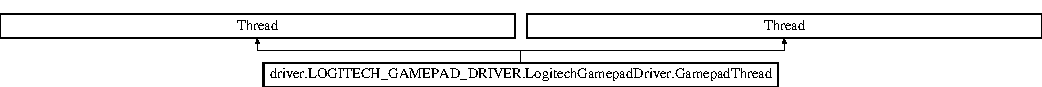
\includegraphics[height=1.166667cm]{classdriver_1_1LOGITECH__GAMEPAD__DRIVER_1_1LogitechGamepadDriver_1_1GamepadThread}
\end{center}
\end{figure}
\subsection*{Public Member Functions}
\begin{DoxyCompactItemize}
\item 
def \hyperlink{classdriver_1_1LOGITECH__GAMEPAD__DRIVER_1_1LogitechGamepadDriver_1_1GamepadThread_aa08ed3fd5770b7518dd3c3672adb37d3}{\+\_\+\+\_\+init\+\_\+\+\_\+}
\item 
def \hyperlink{classdriver_1_1LOGITECH__GAMEPAD__DRIVER_1_1LogitechGamepadDriver_1_1GamepadThread_a1081a12fcf001359ba0755676ef9db77}{run}
\item 
def \hyperlink{classdriver_1_1LOGITECH__GAMEPAD__DRIVER_1_1LogitechGamepadDriver_1_1GamepadThread_aa08ed3fd5770b7518dd3c3672adb37d3}{\+\_\+\+\_\+init\+\_\+\+\_\+}
\item 
def \hyperlink{classdriver_1_1LOGITECH__GAMEPAD__DRIVER_1_1LogitechGamepadDriver_1_1GamepadThread_a1081a12fcf001359ba0755676ef9db77}{run}
\end{DoxyCompactItemize}
\subsection*{Public Attributes}
\begin{DoxyCompactItemize}
\item 
\hyperlink{classdriver_1_1LOGITECH__GAMEPAD__DRIVER_1_1LogitechGamepadDriver_1_1GamepadThread_abede3a32608fc0d308e1cebcbd507eef}{parent}
\item 
\hyperlink{classdriver_1_1LOGITECH__GAMEPAD__DRIVER_1_1LogitechGamepadDriver_1_1GamepadThread_a01174be3f4261cd2dc0510a95907ae24}{num}
\item 
\hyperlink{classdriver_1_1LOGITECH__GAMEPAD__DRIVER_1_1LogitechGamepadDriver_1_1GamepadThread_a013099b962d25f2d0b6ed991527ba55b}{do\+Stuff}
\item 
\hyperlink{classdriver_1_1LOGITECH__GAMEPAD__DRIVER_1_1LogitechGamepadDriver_1_1GamepadThread_aefd0103bf5744b989ad40c8545f35388}{delay}
\end{DoxyCompactItemize}


\subsection{Constructor \& Destructor Documentation}
\hypertarget{classdriver_1_1LOGITECH__GAMEPAD__DRIVER_1_1LogitechGamepadDriver_1_1GamepadThread_aa08ed3fd5770b7518dd3c3672adb37d3}{}\index{driver\+::\+L\+O\+G\+I\+T\+E\+C\+H\+\_\+\+G\+A\+M\+E\+P\+A\+D\+\_\+\+D\+R\+I\+V\+E\+R\+::\+Logitech\+Gamepad\+Driver\+::\+Gamepad\+Thread@{driver\+::\+L\+O\+G\+I\+T\+E\+C\+H\+\_\+\+G\+A\+M\+E\+P\+A\+D\+\_\+\+D\+R\+I\+V\+E\+R\+::\+Logitech\+Gamepad\+Driver\+::\+Gamepad\+Thread}!\+\_\+\+\_\+init\+\_\+\+\_\+@{\+\_\+\+\_\+init\+\_\+\+\_\+}}
\index{\+\_\+\+\_\+init\+\_\+\+\_\+@{\+\_\+\+\_\+init\+\_\+\+\_\+}!driver\+::\+L\+O\+G\+I\+T\+E\+C\+H\+\_\+\+G\+A\+M\+E\+P\+A\+D\+\_\+\+D\+R\+I\+V\+E\+R\+::\+Logitech\+Gamepad\+Driver\+::\+Gamepad\+Thread@{driver\+::\+L\+O\+G\+I\+T\+E\+C\+H\+\_\+\+G\+A\+M\+E\+P\+A\+D\+\_\+\+D\+R\+I\+V\+E\+R\+::\+Logitech\+Gamepad\+Driver\+::\+Gamepad\+Thread}}
\subsubsection[{\+\_\+\+\_\+init\+\_\+\+\_\+}]{\setlength{\rightskip}{0pt plus 5cm}def driver.\+L\+O\+G\+I\+T\+E\+C\+H\+\_\+\+G\+A\+M\+E\+P\+A\+D\+\_\+\+D\+R\+I\+V\+E\+R.\+Logitech\+Gamepad\+Driver.\+Gamepad\+Thread.\+\_\+\+\_\+init\+\_\+\+\_\+ (
\begin{DoxyParamCaption}
\item[{}]{self, }
\item[{}]{parent, }
\item[{}]{num, }
\item[{}]{do\+Stuff, }
\item[{}]{delay}
\end{DoxyParamCaption}
)}\label{classdriver_1_1LOGITECH__GAMEPAD__DRIVER_1_1LogitechGamepadDriver_1_1GamepadThread_aa08ed3fd5770b7518dd3c3672adb37d3}
\hypertarget{classdriver_1_1LOGITECH__GAMEPAD__DRIVER_1_1LogitechGamepadDriver_1_1GamepadThread_aa08ed3fd5770b7518dd3c3672adb37d3}{}\index{driver\+::\+L\+O\+G\+I\+T\+E\+C\+H\+\_\+\+G\+A\+M\+E\+P\+A\+D\+\_\+\+D\+R\+I\+V\+E\+R\+::\+Logitech\+Gamepad\+Driver\+::\+Gamepad\+Thread@{driver\+::\+L\+O\+G\+I\+T\+E\+C\+H\+\_\+\+G\+A\+M\+E\+P\+A\+D\+\_\+\+D\+R\+I\+V\+E\+R\+::\+Logitech\+Gamepad\+Driver\+::\+Gamepad\+Thread}!\+\_\+\+\_\+init\+\_\+\+\_\+@{\+\_\+\+\_\+init\+\_\+\+\_\+}}
\index{\+\_\+\+\_\+init\+\_\+\+\_\+@{\+\_\+\+\_\+init\+\_\+\+\_\+}!driver\+::\+L\+O\+G\+I\+T\+E\+C\+H\+\_\+\+G\+A\+M\+E\+P\+A\+D\+\_\+\+D\+R\+I\+V\+E\+R\+::\+Logitech\+Gamepad\+Driver\+::\+Gamepad\+Thread@{driver\+::\+L\+O\+G\+I\+T\+E\+C\+H\+\_\+\+G\+A\+M\+E\+P\+A\+D\+\_\+\+D\+R\+I\+V\+E\+R\+::\+Logitech\+Gamepad\+Driver\+::\+Gamepad\+Thread}}
\subsubsection[{\+\_\+\+\_\+init\+\_\+\+\_\+}]{\setlength{\rightskip}{0pt plus 5cm}def driver.\+L\+O\+G\+I\+T\+E\+C\+H\+\_\+\+G\+A\+M\+E\+P\+A\+D\+\_\+\+D\+R\+I\+V\+E\+R.\+Logitech\+Gamepad\+Driver.\+Gamepad\+Thread.\+\_\+\+\_\+init\+\_\+\+\_\+ (
\begin{DoxyParamCaption}
\item[{}]{self, }
\item[{}]{parent, }
\item[{}]{num, }
\item[{}]{do\+Stuff, }
\item[{}]{delay}
\end{DoxyParamCaption}
)}\label{classdriver_1_1LOGITECH__GAMEPAD__DRIVER_1_1LogitechGamepadDriver_1_1GamepadThread_aa08ed3fd5770b7518dd3c3672adb37d3}


\subsection{Member Function Documentation}
\hypertarget{classdriver_1_1LOGITECH__GAMEPAD__DRIVER_1_1LogitechGamepadDriver_1_1GamepadThread_a1081a12fcf001359ba0755676ef9db77}{}\index{driver\+::\+L\+O\+G\+I\+T\+E\+C\+H\+\_\+\+G\+A\+M\+E\+P\+A\+D\+\_\+\+D\+R\+I\+V\+E\+R\+::\+Logitech\+Gamepad\+Driver\+::\+Gamepad\+Thread@{driver\+::\+L\+O\+G\+I\+T\+E\+C\+H\+\_\+\+G\+A\+M\+E\+P\+A\+D\+\_\+\+D\+R\+I\+V\+E\+R\+::\+Logitech\+Gamepad\+Driver\+::\+Gamepad\+Thread}!run@{run}}
\index{run@{run}!driver\+::\+L\+O\+G\+I\+T\+E\+C\+H\+\_\+\+G\+A\+M\+E\+P\+A\+D\+\_\+\+D\+R\+I\+V\+E\+R\+::\+Logitech\+Gamepad\+Driver\+::\+Gamepad\+Thread@{driver\+::\+L\+O\+G\+I\+T\+E\+C\+H\+\_\+\+G\+A\+M\+E\+P\+A\+D\+\_\+\+D\+R\+I\+V\+E\+R\+::\+Logitech\+Gamepad\+Driver\+::\+Gamepad\+Thread}}
\subsubsection[{run}]{\setlength{\rightskip}{0pt plus 5cm}def driver.\+L\+O\+G\+I\+T\+E\+C\+H\+\_\+\+G\+A\+M\+E\+P\+A\+D\+\_\+\+D\+R\+I\+V\+E\+R.\+Logitech\+Gamepad\+Driver.\+Gamepad\+Thread.\+run (
\begin{DoxyParamCaption}
\item[{}]{self}
\end{DoxyParamCaption}
)}\label{classdriver_1_1LOGITECH__GAMEPAD__DRIVER_1_1LogitechGamepadDriver_1_1GamepadThread_a1081a12fcf001359ba0755676ef9db77}
\hypertarget{classdriver_1_1LOGITECH__GAMEPAD__DRIVER_1_1LogitechGamepadDriver_1_1GamepadThread_a1081a12fcf001359ba0755676ef9db77}{}\index{driver\+::\+L\+O\+G\+I\+T\+E\+C\+H\+\_\+\+G\+A\+M\+E\+P\+A\+D\+\_\+\+D\+R\+I\+V\+E\+R\+::\+Logitech\+Gamepad\+Driver\+::\+Gamepad\+Thread@{driver\+::\+L\+O\+G\+I\+T\+E\+C\+H\+\_\+\+G\+A\+M\+E\+P\+A\+D\+\_\+\+D\+R\+I\+V\+E\+R\+::\+Logitech\+Gamepad\+Driver\+::\+Gamepad\+Thread}!run@{run}}
\index{run@{run}!driver\+::\+L\+O\+G\+I\+T\+E\+C\+H\+\_\+\+G\+A\+M\+E\+P\+A\+D\+\_\+\+D\+R\+I\+V\+E\+R\+::\+Logitech\+Gamepad\+Driver\+::\+Gamepad\+Thread@{driver\+::\+L\+O\+G\+I\+T\+E\+C\+H\+\_\+\+G\+A\+M\+E\+P\+A\+D\+\_\+\+D\+R\+I\+V\+E\+R\+::\+Logitech\+Gamepad\+Driver\+::\+Gamepad\+Thread}}
\subsubsection[{run}]{\setlength{\rightskip}{0pt plus 5cm}def driver.\+L\+O\+G\+I\+T\+E\+C\+H\+\_\+\+G\+A\+M\+E\+P\+A\+D\+\_\+\+D\+R\+I\+V\+E\+R.\+Logitech\+Gamepad\+Driver.\+Gamepad\+Thread.\+run (
\begin{DoxyParamCaption}
\item[{}]{self}
\end{DoxyParamCaption}
)}\label{classdriver_1_1LOGITECH__GAMEPAD__DRIVER_1_1LogitechGamepadDriver_1_1GamepadThread_a1081a12fcf001359ba0755676ef9db77}


\subsection{Member Data Documentation}
\hypertarget{classdriver_1_1LOGITECH__GAMEPAD__DRIVER_1_1LogitechGamepadDriver_1_1GamepadThread_aefd0103bf5744b989ad40c8545f35388}{}\index{driver\+::\+L\+O\+G\+I\+T\+E\+C\+H\+\_\+\+G\+A\+M\+E\+P\+A\+D\+\_\+\+D\+R\+I\+V\+E\+R\+::\+Logitech\+Gamepad\+Driver\+::\+Gamepad\+Thread@{driver\+::\+L\+O\+G\+I\+T\+E\+C\+H\+\_\+\+G\+A\+M\+E\+P\+A\+D\+\_\+\+D\+R\+I\+V\+E\+R\+::\+Logitech\+Gamepad\+Driver\+::\+Gamepad\+Thread}!delay@{delay}}
\index{delay@{delay}!driver\+::\+L\+O\+G\+I\+T\+E\+C\+H\+\_\+\+G\+A\+M\+E\+P\+A\+D\+\_\+\+D\+R\+I\+V\+E\+R\+::\+Logitech\+Gamepad\+Driver\+::\+Gamepad\+Thread@{driver\+::\+L\+O\+G\+I\+T\+E\+C\+H\+\_\+\+G\+A\+M\+E\+P\+A\+D\+\_\+\+D\+R\+I\+V\+E\+R\+::\+Logitech\+Gamepad\+Driver\+::\+Gamepad\+Thread}}
\subsubsection[{delay}]{\setlength{\rightskip}{0pt plus 5cm}driver.\+L\+O\+G\+I\+T\+E\+C\+H\+\_\+\+G\+A\+M\+E\+P\+A\+D\+\_\+\+D\+R\+I\+V\+E\+R.\+Logitech\+Gamepad\+Driver.\+Gamepad\+Thread.\+delay}\label{classdriver_1_1LOGITECH__GAMEPAD__DRIVER_1_1LogitechGamepadDriver_1_1GamepadThread_aefd0103bf5744b989ad40c8545f35388}
\hypertarget{classdriver_1_1LOGITECH__GAMEPAD__DRIVER_1_1LogitechGamepadDriver_1_1GamepadThread_a013099b962d25f2d0b6ed991527ba55b}{}\index{driver\+::\+L\+O\+G\+I\+T\+E\+C\+H\+\_\+\+G\+A\+M\+E\+P\+A\+D\+\_\+\+D\+R\+I\+V\+E\+R\+::\+Logitech\+Gamepad\+Driver\+::\+Gamepad\+Thread@{driver\+::\+L\+O\+G\+I\+T\+E\+C\+H\+\_\+\+G\+A\+M\+E\+P\+A\+D\+\_\+\+D\+R\+I\+V\+E\+R\+::\+Logitech\+Gamepad\+Driver\+::\+Gamepad\+Thread}!do\+Stuff@{do\+Stuff}}
\index{do\+Stuff@{do\+Stuff}!driver\+::\+L\+O\+G\+I\+T\+E\+C\+H\+\_\+\+G\+A\+M\+E\+P\+A\+D\+\_\+\+D\+R\+I\+V\+E\+R\+::\+Logitech\+Gamepad\+Driver\+::\+Gamepad\+Thread@{driver\+::\+L\+O\+G\+I\+T\+E\+C\+H\+\_\+\+G\+A\+M\+E\+P\+A\+D\+\_\+\+D\+R\+I\+V\+E\+R\+::\+Logitech\+Gamepad\+Driver\+::\+Gamepad\+Thread}}
\subsubsection[{do\+Stuff}]{\setlength{\rightskip}{0pt plus 5cm}driver.\+L\+O\+G\+I\+T\+E\+C\+H\+\_\+\+G\+A\+M\+E\+P\+A\+D\+\_\+\+D\+R\+I\+V\+E\+R.\+Logitech\+Gamepad\+Driver.\+Gamepad\+Thread.\+do\+Stuff}\label{classdriver_1_1LOGITECH__GAMEPAD__DRIVER_1_1LogitechGamepadDriver_1_1GamepadThread_a013099b962d25f2d0b6ed991527ba55b}
\hypertarget{classdriver_1_1LOGITECH__GAMEPAD__DRIVER_1_1LogitechGamepadDriver_1_1GamepadThread_a01174be3f4261cd2dc0510a95907ae24}{}\index{driver\+::\+L\+O\+G\+I\+T\+E\+C\+H\+\_\+\+G\+A\+M\+E\+P\+A\+D\+\_\+\+D\+R\+I\+V\+E\+R\+::\+Logitech\+Gamepad\+Driver\+::\+Gamepad\+Thread@{driver\+::\+L\+O\+G\+I\+T\+E\+C\+H\+\_\+\+G\+A\+M\+E\+P\+A\+D\+\_\+\+D\+R\+I\+V\+E\+R\+::\+Logitech\+Gamepad\+Driver\+::\+Gamepad\+Thread}!num@{num}}
\index{num@{num}!driver\+::\+L\+O\+G\+I\+T\+E\+C\+H\+\_\+\+G\+A\+M\+E\+P\+A\+D\+\_\+\+D\+R\+I\+V\+E\+R\+::\+Logitech\+Gamepad\+Driver\+::\+Gamepad\+Thread@{driver\+::\+L\+O\+G\+I\+T\+E\+C\+H\+\_\+\+G\+A\+M\+E\+P\+A\+D\+\_\+\+D\+R\+I\+V\+E\+R\+::\+Logitech\+Gamepad\+Driver\+::\+Gamepad\+Thread}}
\subsubsection[{num}]{\setlength{\rightskip}{0pt plus 5cm}driver.\+L\+O\+G\+I\+T\+E\+C\+H\+\_\+\+G\+A\+M\+E\+P\+A\+D\+\_\+\+D\+R\+I\+V\+E\+R.\+Logitech\+Gamepad\+Driver.\+Gamepad\+Thread.\+num}\label{classdriver_1_1LOGITECH__GAMEPAD__DRIVER_1_1LogitechGamepadDriver_1_1GamepadThread_a01174be3f4261cd2dc0510a95907ae24}
\hypertarget{classdriver_1_1LOGITECH__GAMEPAD__DRIVER_1_1LogitechGamepadDriver_1_1GamepadThread_abede3a32608fc0d308e1cebcbd507eef}{}\index{driver\+::\+L\+O\+G\+I\+T\+E\+C\+H\+\_\+\+G\+A\+M\+E\+P\+A\+D\+\_\+\+D\+R\+I\+V\+E\+R\+::\+Logitech\+Gamepad\+Driver\+::\+Gamepad\+Thread@{driver\+::\+L\+O\+G\+I\+T\+E\+C\+H\+\_\+\+G\+A\+M\+E\+P\+A\+D\+\_\+\+D\+R\+I\+V\+E\+R\+::\+Logitech\+Gamepad\+Driver\+::\+Gamepad\+Thread}!parent@{parent}}
\index{parent@{parent}!driver\+::\+L\+O\+G\+I\+T\+E\+C\+H\+\_\+\+G\+A\+M\+E\+P\+A\+D\+\_\+\+D\+R\+I\+V\+E\+R\+::\+Logitech\+Gamepad\+Driver\+::\+Gamepad\+Thread@{driver\+::\+L\+O\+G\+I\+T\+E\+C\+H\+\_\+\+G\+A\+M\+E\+P\+A\+D\+\_\+\+D\+R\+I\+V\+E\+R\+::\+Logitech\+Gamepad\+Driver\+::\+Gamepad\+Thread}}
\subsubsection[{parent}]{\setlength{\rightskip}{0pt plus 5cm}driver.\+L\+O\+G\+I\+T\+E\+C\+H\+\_\+\+G\+A\+M\+E\+P\+A\+D\+\_\+\+D\+R\+I\+V\+E\+R.\+Logitech\+Gamepad\+Driver.\+Gamepad\+Thread.\+parent}\label{classdriver_1_1LOGITECH__GAMEPAD__DRIVER_1_1LogitechGamepadDriver_1_1GamepadThread_abede3a32608fc0d308e1cebcbd507eef}


The documentation for this class was generated from the following file\+:\begin{DoxyCompactItemize}
\item 
build/lib.\+linux-\/x86\+\_\+64-\/2.\+7/driver/\hyperlink{build_2lib_8linux-x86__64-2_87_2driver_2LOGITECH__GAMEPAD__DRIVER_8py}{L\+O\+G\+I\+T\+E\+C\+H\+\_\+\+G\+A\+M\+E\+P\+A\+D\+\_\+\+D\+R\+I\+V\+E\+R.\+py}\end{DoxyCompactItemize}

\hypertarget{classnetwork_1_1I2C_1_1i2c}{}\section{network.\+I2\+C.\+i2c Class Reference}
\label{classnetwork_1_1I2C_1_1i2c}\index{network.\+I2\+C.\+i2c@{network.\+I2\+C.\+i2c}}
\subsection*{Public Member Functions}
\begin{DoxyCompactItemize}
\item 
def \hyperlink{classnetwork_1_1I2C_1_1i2c_a4c67f9c04de709214b672c552e1216dd}{\+\_\+\+\_\+init\+\_\+\+\_\+}
\item 
def \hyperlink{classnetwork_1_1I2C_1_1i2c_a88e5789401d5b33a462412c38f5b1c2c}{write\+\_\+cmd}
\item 
def \hyperlink{classnetwork_1_1I2C_1_1i2c_a5254eef4f67541372a8e0e70bd846593}{write\+\_\+cmd\+\_\+arg}
\item 
def \hyperlink{classnetwork_1_1I2C_1_1i2c_ae2eb38185381cb2307b3f3ca5cd819af}{write\+\_\+block\+\_\+data}
\item 
def \hyperlink{classnetwork_1_1I2C_1_1i2c_a92d95fdee4c3dce774e083f566436c84}{read}
\item 
def \hyperlink{classnetwork_1_1I2C_1_1i2c_a57e1f004ef70ea82c9410392662e7412}{read\+\_\+data}
\item 
def \hyperlink{classnetwork_1_1I2C_1_1i2c_a105b6381dad9576d206794d99ac31d6d}{read\+\_\+block\+\_\+data}
\item 
def \hyperlink{classnetwork_1_1I2C_1_1i2c_a4c67f9c04de709214b672c552e1216dd}{\+\_\+\+\_\+init\+\_\+\+\_\+}
\item 
def \hyperlink{classnetwork_1_1I2C_1_1i2c_a88e5789401d5b33a462412c38f5b1c2c}{write\+\_\+cmd}
\item 
def \hyperlink{classnetwork_1_1I2C_1_1i2c_a5254eef4f67541372a8e0e70bd846593}{write\+\_\+cmd\+\_\+arg}
\item 
def \hyperlink{classnetwork_1_1I2C_1_1i2c_ae2eb38185381cb2307b3f3ca5cd819af}{write\+\_\+block\+\_\+data}
\item 
def \hyperlink{classnetwork_1_1I2C_1_1i2c_a92d95fdee4c3dce774e083f566436c84}{read}
\item 
def \hyperlink{classnetwork_1_1I2C_1_1i2c_a57e1f004ef70ea82c9410392662e7412}{read\+\_\+data}
\item 
def \hyperlink{classnetwork_1_1I2C_1_1i2c_a105b6381dad9576d206794d99ac31d6d}{read\+\_\+block\+\_\+data}
\end{DoxyCompactItemize}
\subsection*{Public Attributes}
\begin{DoxyCompactItemize}
\item 
\hyperlink{classnetwork_1_1I2C_1_1i2c_a2b5c11f2acf663fa0349d18714a60db6}{addr}
\item 
\hyperlink{classnetwork_1_1I2C_1_1i2c_a60c56af8dc524a1ef92e36e97d8927c7}{bus}
\end{DoxyCompactItemize}


\subsection{Constructor \& Destructor Documentation}
\hypertarget{classnetwork_1_1I2C_1_1i2c_a4c67f9c04de709214b672c552e1216dd}{}\index{network\+::\+I2\+C\+::i2c@{network\+::\+I2\+C\+::i2c}!\+\_\+\+\_\+init\+\_\+\+\_\+@{\+\_\+\+\_\+init\+\_\+\+\_\+}}
\index{\+\_\+\+\_\+init\+\_\+\+\_\+@{\+\_\+\+\_\+init\+\_\+\+\_\+}!network\+::\+I2\+C\+::i2c@{network\+::\+I2\+C\+::i2c}}
\subsubsection[{\+\_\+\+\_\+init\+\_\+\+\_\+}]{\setlength{\rightskip}{0pt plus 5cm}def network.\+I2\+C.\+i2c.\+\_\+\+\_\+init\+\_\+\+\_\+ (
\begin{DoxyParamCaption}
\item[{}]{self, }
\item[{}]{addr, }
\item[{}]{port = {\ttfamily 1}}
\end{DoxyParamCaption}
)}\label{classnetwork_1_1I2C_1_1i2c_a4c67f9c04de709214b672c552e1216dd}
\hypertarget{classnetwork_1_1I2C_1_1i2c_a4c67f9c04de709214b672c552e1216dd}{}\index{network\+::\+I2\+C\+::i2c@{network\+::\+I2\+C\+::i2c}!\+\_\+\+\_\+init\+\_\+\+\_\+@{\+\_\+\+\_\+init\+\_\+\+\_\+}}
\index{\+\_\+\+\_\+init\+\_\+\+\_\+@{\+\_\+\+\_\+init\+\_\+\+\_\+}!network\+::\+I2\+C\+::i2c@{network\+::\+I2\+C\+::i2c}}
\subsubsection[{\+\_\+\+\_\+init\+\_\+\+\_\+}]{\setlength{\rightskip}{0pt plus 5cm}def network.\+I2\+C.\+i2c.\+\_\+\+\_\+init\+\_\+\+\_\+ (
\begin{DoxyParamCaption}
\item[{}]{self, }
\item[{}]{addr, }
\item[{}]{port = {\ttfamily 1}}
\end{DoxyParamCaption}
)}\label{classnetwork_1_1I2C_1_1i2c_a4c67f9c04de709214b672c552e1216dd}


\subsection{Member Function Documentation}
\hypertarget{classnetwork_1_1I2C_1_1i2c_a92d95fdee4c3dce774e083f566436c84}{}\index{network\+::\+I2\+C\+::i2c@{network\+::\+I2\+C\+::i2c}!read@{read}}
\index{read@{read}!network\+::\+I2\+C\+::i2c@{network\+::\+I2\+C\+::i2c}}
\subsubsection[{read}]{\setlength{\rightskip}{0pt plus 5cm}def network.\+I2\+C.\+i2c.\+read (
\begin{DoxyParamCaption}
\item[{}]{self}
\end{DoxyParamCaption}
)}\label{classnetwork_1_1I2C_1_1i2c_a92d95fdee4c3dce774e083f566436c84}
\hypertarget{classnetwork_1_1I2C_1_1i2c_a92d95fdee4c3dce774e083f566436c84}{}\index{network\+::\+I2\+C\+::i2c@{network\+::\+I2\+C\+::i2c}!read@{read}}
\index{read@{read}!network\+::\+I2\+C\+::i2c@{network\+::\+I2\+C\+::i2c}}
\subsubsection[{read}]{\setlength{\rightskip}{0pt plus 5cm}def network.\+I2\+C.\+i2c.\+read (
\begin{DoxyParamCaption}
\item[{}]{self}
\end{DoxyParamCaption}
)}\label{classnetwork_1_1I2C_1_1i2c_a92d95fdee4c3dce774e083f566436c84}
\hypertarget{classnetwork_1_1I2C_1_1i2c_a105b6381dad9576d206794d99ac31d6d}{}\index{network\+::\+I2\+C\+::i2c@{network\+::\+I2\+C\+::i2c}!read\+\_\+block\+\_\+data@{read\+\_\+block\+\_\+data}}
\index{read\+\_\+block\+\_\+data@{read\+\_\+block\+\_\+data}!network\+::\+I2\+C\+::i2c@{network\+::\+I2\+C\+::i2c}}
\subsubsection[{read\+\_\+block\+\_\+data}]{\setlength{\rightskip}{0pt plus 5cm}def network.\+I2\+C.\+i2c.\+read\+\_\+block\+\_\+data (
\begin{DoxyParamCaption}
\item[{}]{self, }
\item[{}]{cmd}
\end{DoxyParamCaption}
)}\label{classnetwork_1_1I2C_1_1i2c_a105b6381dad9576d206794d99ac31d6d}
\hypertarget{classnetwork_1_1I2C_1_1i2c_a105b6381dad9576d206794d99ac31d6d}{}\index{network\+::\+I2\+C\+::i2c@{network\+::\+I2\+C\+::i2c}!read\+\_\+block\+\_\+data@{read\+\_\+block\+\_\+data}}
\index{read\+\_\+block\+\_\+data@{read\+\_\+block\+\_\+data}!network\+::\+I2\+C\+::i2c@{network\+::\+I2\+C\+::i2c}}
\subsubsection[{read\+\_\+block\+\_\+data}]{\setlength{\rightskip}{0pt plus 5cm}def network.\+I2\+C.\+i2c.\+read\+\_\+block\+\_\+data (
\begin{DoxyParamCaption}
\item[{}]{self, }
\item[{}]{cmd}
\end{DoxyParamCaption}
)}\label{classnetwork_1_1I2C_1_1i2c_a105b6381dad9576d206794d99ac31d6d}
\hypertarget{classnetwork_1_1I2C_1_1i2c_a57e1f004ef70ea82c9410392662e7412}{}\index{network\+::\+I2\+C\+::i2c@{network\+::\+I2\+C\+::i2c}!read\+\_\+data@{read\+\_\+data}}
\index{read\+\_\+data@{read\+\_\+data}!network\+::\+I2\+C\+::i2c@{network\+::\+I2\+C\+::i2c}}
\subsubsection[{read\+\_\+data}]{\setlength{\rightskip}{0pt plus 5cm}def network.\+I2\+C.\+i2c.\+read\+\_\+data (
\begin{DoxyParamCaption}
\item[{}]{self, }
\item[{}]{cmd}
\end{DoxyParamCaption}
)}\label{classnetwork_1_1I2C_1_1i2c_a57e1f004ef70ea82c9410392662e7412}
\hypertarget{classnetwork_1_1I2C_1_1i2c_a57e1f004ef70ea82c9410392662e7412}{}\index{network\+::\+I2\+C\+::i2c@{network\+::\+I2\+C\+::i2c}!read\+\_\+data@{read\+\_\+data}}
\index{read\+\_\+data@{read\+\_\+data}!network\+::\+I2\+C\+::i2c@{network\+::\+I2\+C\+::i2c}}
\subsubsection[{read\+\_\+data}]{\setlength{\rightskip}{0pt plus 5cm}def network.\+I2\+C.\+i2c.\+read\+\_\+data (
\begin{DoxyParamCaption}
\item[{}]{self, }
\item[{}]{cmd}
\end{DoxyParamCaption}
)}\label{classnetwork_1_1I2C_1_1i2c_a57e1f004ef70ea82c9410392662e7412}
\hypertarget{classnetwork_1_1I2C_1_1i2c_ae2eb38185381cb2307b3f3ca5cd819af}{}\index{network\+::\+I2\+C\+::i2c@{network\+::\+I2\+C\+::i2c}!write\+\_\+block\+\_\+data@{write\+\_\+block\+\_\+data}}
\index{write\+\_\+block\+\_\+data@{write\+\_\+block\+\_\+data}!network\+::\+I2\+C\+::i2c@{network\+::\+I2\+C\+::i2c}}
\subsubsection[{write\+\_\+block\+\_\+data}]{\setlength{\rightskip}{0pt plus 5cm}def network.\+I2\+C.\+i2c.\+write\+\_\+block\+\_\+data (
\begin{DoxyParamCaption}
\item[{}]{self, }
\item[{}]{cmd, }
\item[{}]{data}
\end{DoxyParamCaption}
)}\label{classnetwork_1_1I2C_1_1i2c_ae2eb38185381cb2307b3f3ca5cd819af}
\hypertarget{classnetwork_1_1I2C_1_1i2c_ae2eb38185381cb2307b3f3ca5cd819af}{}\index{network\+::\+I2\+C\+::i2c@{network\+::\+I2\+C\+::i2c}!write\+\_\+block\+\_\+data@{write\+\_\+block\+\_\+data}}
\index{write\+\_\+block\+\_\+data@{write\+\_\+block\+\_\+data}!network\+::\+I2\+C\+::i2c@{network\+::\+I2\+C\+::i2c}}
\subsubsection[{write\+\_\+block\+\_\+data}]{\setlength{\rightskip}{0pt plus 5cm}def network.\+I2\+C.\+i2c.\+write\+\_\+block\+\_\+data (
\begin{DoxyParamCaption}
\item[{}]{self, }
\item[{}]{cmd, }
\item[{}]{data}
\end{DoxyParamCaption}
)}\label{classnetwork_1_1I2C_1_1i2c_ae2eb38185381cb2307b3f3ca5cd819af}
\hypertarget{classnetwork_1_1I2C_1_1i2c_a88e5789401d5b33a462412c38f5b1c2c}{}\index{network\+::\+I2\+C\+::i2c@{network\+::\+I2\+C\+::i2c}!write\+\_\+cmd@{write\+\_\+cmd}}
\index{write\+\_\+cmd@{write\+\_\+cmd}!network\+::\+I2\+C\+::i2c@{network\+::\+I2\+C\+::i2c}}
\subsubsection[{write\+\_\+cmd}]{\setlength{\rightskip}{0pt plus 5cm}def network.\+I2\+C.\+i2c.\+write\+\_\+cmd (
\begin{DoxyParamCaption}
\item[{}]{self, }
\item[{}]{cmd}
\end{DoxyParamCaption}
)}\label{classnetwork_1_1I2C_1_1i2c_a88e5789401d5b33a462412c38f5b1c2c}
\hypertarget{classnetwork_1_1I2C_1_1i2c_a88e5789401d5b33a462412c38f5b1c2c}{}\index{network\+::\+I2\+C\+::i2c@{network\+::\+I2\+C\+::i2c}!write\+\_\+cmd@{write\+\_\+cmd}}
\index{write\+\_\+cmd@{write\+\_\+cmd}!network\+::\+I2\+C\+::i2c@{network\+::\+I2\+C\+::i2c}}
\subsubsection[{write\+\_\+cmd}]{\setlength{\rightskip}{0pt plus 5cm}def network.\+I2\+C.\+i2c.\+write\+\_\+cmd (
\begin{DoxyParamCaption}
\item[{}]{self, }
\item[{}]{cmd}
\end{DoxyParamCaption}
)}\label{classnetwork_1_1I2C_1_1i2c_a88e5789401d5b33a462412c38f5b1c2c}
\hypertarget{classnetwork_1_1I2C_1_1i2c_a5254eef4f67541372a8e0e70bd846593}{}\index{network\+::\+I2\+C\+::i2c@{network\+::\+I2\+C\+::i2c}!write\+\_\+cmd\+\_\+arg@{write\+\_\+cmd\+\_\+arg}}
\index{write\+\_\+cmd\+\_\+arg@{write\+\_\+cmd\+\_\+arg}!network\+::\+I2\+C\+::i2c@{network\+::\+I2\+C\+::i2c}}
\subsubsection[{write\+\_\+cmd\+\_\+arg}]{\setlength{\rightskip}{0pt plus 5cm}def network.\+I2\+C.\+i2c.\+write\+\_\+cmd\+\_\+arg (
\begin{DoxyParamCaption}
\item[{}]{self, }
\item[{}]{cmd, }
\item[{}]{data}
\end{DoxyParamCaption}
)}\label{classnetwork_1_1I2C_1_1i2c_a5254eef4f67541372a8e0e70bd846593}
\hypertarget{classnetwork_1_1I2C_1_1i2c_a5254eef4f67541372a8e0e70bd846593}{}\index{network\+::\+I2\+C\+::i2c@{network\+::\+I2\+C\+::i2c}!write\+\_\+cmd\+\_\+arg@{write\+\_\+cmd\+\_\+arg}}
\index{write\+\_\+cmd\+\_\+arg@{write\+\_\+cmd\+\_\+arg}!network\+::\+I2\+C\+::i2c@{network\+::\+I2\+C\+::i2c}}
\subsubsection[{write\+\_\+cmd\+\_\+arg}]{\setlength{\rightskip}{0pt plus 5cm}def network.\+I2\+C.\+i2c.\+write\+\_\+cmd\+\_\+arg (
\begin{DoxyParamCaption}
\item[{}]{self, }
\item[{}]{cmd, }
\item[{}]{data}
\end{DoxyParamCaption}
)}\label{classnetwork_1_1I2C_1_1i2c_a5254eef4f67541372a8e0e70bd846593}


\subsection{Member Data Documentation}
\hypertarget{classnetwork_1_1I2C_1_1i2c_a2b5c11f2acf663fa0349d18714a60db6}{}\index{network\+::\+I2\+C\+::i2c@{network\+::\+I2\+C\+::i2c}!addr@{addr}}
\index{addr@{addr}!network\+::\+I2\+C\+::i2c@{network\+::\+I2\+C\+::i2c}}
\subsubsection[{addr}]{\setlength{\rightskip}{0pt plus 5cm}network.\+I2\+C.\+i2c.\+addr}\label{classnetwork_1_1I2C_1_1i2c_a2b5c11f2acf663fa0349d18714a60db6}
\hypertarget{classnetwork_1_1I2C_1_1i2c_a60c56af8dc524a1ef92e36e97d8927c7}{}\index{network\+::\+I2\+C\+::i2c@{network\+::\+I2\+C\+::i2c}!bus@{bus}}
\index{bus@{bus}!network\+::\+I2\+C\+::i2c@{network\+::\+I2\+C\+::i2c}}
\subsubsection[{bus}]{\setlength{\rightskip}{0pt plus 5cm}network.\+I2\+C.\+i2c.\+bus}\label{classnetwork_1_1I2C_1_1i2c_a60c56af8dc524a1ef92e36e97d8927c7}


The documentation for this class was generated from the following file\+:\begin{DoxyCompactItemize}
\item 
G\+I\+T-\/\+C\+O\+P\+Y/\+Software/network/\hyperlink{GIT-COPY_2Software_2network_2I2C_8py}{I2\+C.\+py}\end{DoxyCompactItemize}

\hypertarget{classdriver_1_1i2c__lib_1_1i2c__device}{}\section{driver.\+i2c\+\_\+lib.\+i2c\+\_\+device Class Reference}
\label{classdriver_1_1i2c__lib_1_1i2c__device}\index{driver.\+i2c\+\_\+lib.\+i2c\+\_\+device@{driver.\+i2c\+\_\+lib.\+i2c\+\_\+device}}
\subsection*{Public Member Functions}
\begin{DoxyCompactItemize}
\item 
\hypertarget{classdriver_1_1i2c__lib_1_1i2c__device_a6f4de0589e9fc9d80dfcbe78764adca6}{}def {\bfseries \+\_\+\+\_\+init\+\_\+\+\_\+}\label{classdriver_1_1i2c__lib_1_1i2c__device_a6f4de0589e9fc9d80dfcbe78764adca6}

\item 
\hypertarget{classdriver_1_1i2c__lib_1_1i2c__device_a4793439f363c2b22a7f3beae6074f755}{}def {\bfseries write\+\_\+cmd}\label{classdriver_1_1i2c__lib_1_1i2c__device_a4793439f363c2b22a7f3beae6074f755}

\item 
\hypertarget{classdriver_1_1i2c__lib_1_1i2c__device_ae998e6b6651a038c5b5466ae941e0eb8}{}def {\bfseries write\+\_\+cmd\+\_\+arg}\label{classdriver_1_1i2c__lib_1_1i2c__device_ae998e6b6651a038c5b5466ae941e0eb8}

\item 
\hypertarget{classdriver_1_1i2c__lib_1_1i2c__device_ae270018219f2f96ec9e37e36065d2edc}{}def {\bfseries write\+\_\+block\+\_\+data}\label{classdriver_1_1i2c__lib_1_1i2c__device_ae270018219f2f96ec9e37e36065d2edc}

\item 
\hypertarget{classdriver_1_1i2c__lib_1_1i2c__device_a9a8d9b4cc3d3890baa0738c9fa60ef4b}{}def {\bfseries read}\label{classdriver_1_1i2c__lib_1_1i2c__device_a9a8d9b4cc3d3890baa0738c9fa60ef4b}

\item 
\hypertarget{classdriver_1_1i2c__lib_1_1i2c__device_a7960797223c6a315d764f8b1ff11a8f2}{}def {\bfseries read\+\_\+data}\label{classdriver_1_1i2c__lib_1_1i2c__device_a7960797223c6a315d764f8b1ff11a8f2}

\item 
\hypertarget{classdriver_1_1i2c__lib_1_1i2c__device_ad837253a1137bd4ae725f80640ace947}{}def {\bfseries read\+\_\+block\+\_\+data}\label{classdriver_1_1i2c__lib_1_1i2c__device_ad837253a1137bd4ae725f80640ace947}

\end{DoxyCompactItemize}
\subsection*{Public Attributes}
\begin{DoxyCompactItemize}
\item 
\hypertarget{classdriver_1_1i2c__lib_1_1i2c__device_a9cfbff86867d526e3bcb5213d80b6f2c}{}{\bfseries addr}\label{classdriver_1_1i2c__lib_1_1i2c__device_a9cfbff86867d526e3bcb5213d80b6f2c}

\item 
\hypertarget{classdriver_1_1i2c__lib_1_1i2c__device_ac57614bbc2affcaf48f890e8a79c1e96}{}{\bfseries bus}\label{classdriver_1_1i2c__lib_1_1i2c__device_ac57614bbc2affcaf48f890e8a79c1e96}

\end{DoxyCompactItemize}


The documentation for this class was generated from the following file\+:\begin{DoxyCompactItemize}
\item 
i2c\+\_\+lib.\+py\end{DoxyCompactItemize}

\hypertarget{classinterface_1_1INTERFACE__CORE_1_1interface}{}\section{interface.\+I\+N\+T\+E\+R\+F\+A\+C\+E\+\_\+\+C\+O\+R\+E.\+interface Class Reference}
\label{classinterface_1_1INTERFACE__CORE_1_1interface}\index{interface.\+I\+N\+T\+E\+R\+F\+A\+C\+E\+\_\+\+C\+O\+R\+E.\+interface@{interface.\+I\+N\+T\+E\+R\+F\+A\+C\+E\+\_\+\+C\+O\+R\+E.\+interface}}
Inheritance diagram for interface.\+I\+N\+T\+E\+R\+F\+A\+C\+E\+\_\+\+C\+O\+R\+E.\+interface\+:\begin{figure}[H]
\begin{center}
\leavevmode
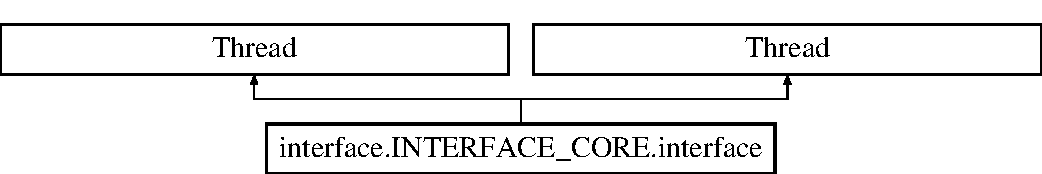
\includegraphics[height=2.000000cm]{classinterface_1_1INTERFACE__CORE_1_1interface}
\end{center}
\end{figure}
\subsection*{Public Member Functions}
\begin{DoxyCompactItemize}
\item 
def \hyperlink{classinterface_1_1INTERFACE__CORE_1_1interface_a96fbbdd17999b9eb5430336f475c91ad}{\+\_\+\+\_\+init\+\_\+\+\_\+}
\item 
def \hyperlink{classinterface_1_1INTERFACE__CORE_1_1interface_a9e590fb5bf7673a7c77027f4ded29abb}{add\+Model}
\item 
def \hyperlink{classinterface_1_1INTERFACE__CORE_1_1interface_a7876b4f6147630ed64bde3864aed78c0}{add\+Interface}
\item 
def \hyperlink{classinterface_1_1INTERFACE__CORE_1_1interface_a54871907738176848a480584557cb65b}{add\+Driver}
\item 
def \hyperlink{classinterface_1_1INTERFACE__CORE_1_1interface_afca54b5f57d67ed5ba8b4dc110fa2647}{update}
\item 
def \hyperlink{classinterface_1_1INTERFACE__CORE_1_1interface_a2ba0b1d20f8ee0bf50b468bb82e91d4d}{run}
\item 
def \hyperlink{classinterface_1_1INTERFACE__CORE_1_1interface_a96fbbdd17999b9eb5430336f475c91ad}{\+\_\+\+\_\+init\+\_\+\+\_\+}
\item 
def \hyperlink{classinterface_1_1INTERFACE__CORE_1_1interface_a9e590fb5bf7673a7c77027f4ded29abb}{add\+Model}
\item 
def \hyperlink{classinterface_1_1INTERFACE__CORE_1_1interface_a7876b4f6147630ed64bde3864aed78c0}{add\+Interface}
\item 
def \hyperlink{classinterface_1_1INTERFACE__CORE_1_1interface_a54871907738176848a480584557cb65b}{add\+Driver}
\item 
def \hyperlink{classinterface_1_1INTERFACE__CORE_1_1interface_afca54b5f57d67ed5ba8b4dc110fa2647}{update}
\item 
def \hyperlink{classinterface_1_1INTERFACE__CORE_1_1interface_a2ba0b1d20f8ee0bf50b468bb82e91d4d}{run}
\end{DoxyCompactItemize}
\subsection*{Public Attributes}
\begin{DoxyCompactItemize}
\item 
\hyperlink{classinterface_1_1INTERFACE__CORE_1_1interface_a360e2dd2c4bc4c873884831bfaa86582}{interfaces}
\item 
\hyperlink{classinterface_1_1INTERFACE__CORE_1_1interface_a15823225e3f265a09e00938b28ac12da}{models}
\item 
\hyperlink{classinterface_1_1INTERFACE__CORE_1_1interface_accf9df0d1460957144aa70522fa66a6c}{drivers}
\end{DoxyCompactItemize}


\subsection{Constructor \& Destructor Documentation}
\hypertarget{classinterface_1_1INTERFACE__CORE_1_1interface_a96fbbdd17999b9eb5430336f475c91ad}{}\index{interface\+::\+I\+N\+T\+E\+R\+F\+A\+C\+E\+\_\+\+C\+O\+R\+E\+::interface@{interface\+::\+I\+N\+T\+E\+R\+F\+A\+C\+E\+\_\+\+C\+O\+R\+E\+::interface}!\+\_\+\+\_\+init\+\_\+\+\_\+@{\+\_\+\+\_\+init\+\_\+\+\_\+}}
\index{\+\_\+\+\_\+init\+\_\+\+\_\+@{\+\_\+\+\_\+init\+\_\+\+\_\+}!interface\+::\+I\+N\+T\+E\+R\+F\+A\+C\+E\+\_\+\+C\+O\+R\+E\+::interface@{interface\+::\+I\+N\+T\+E\+R\+F\+A\+C\+E\+\_\+\+C\+O\+R\+E\+::interface}}
\subsubsection[{\+\_\+\+\_\+init\+\_\+\+\_\+}]{\setlength{\rightskip}{0pt plus 5cm}def interface.\+I\+N\+T\+E\+R\+F\+A\+C\+E\+\_\+\+C\+O\+R\+E.\+interface.\+\_\+\+\_\+init\+\_\+\+\_\+ (
\begin{DoxyParamCaption}
\item[{}]{self, }
\item[{}]{name}
\end{DoxyParamCaption}
)}\label{classinterface_1_1INTERFACE__CORE_1_1interface_a96fbbdd17999b9eb5430336f475c91ad}
\hypertarget{classinterface_1_1INTERFACE__CORE_1_1interface_a96fbbdd17999b9eb5430336f475c91ad}{}\index{interface\+::\+I\+N\+T\+E\+R\+F\+A\+C\+E\+\_\+\+C\+O\+R\+E\+::interface@{interface\+::\+I\+N\+T\+E\+R\+F\+A\+C\+E\+\_\+\+C\+O\+R\+E\+::interface}!\+\_\+\+\_\+init\+\_\+\+\_\+@{\+\_\+\+\_\+init\+\_\+\+\_\+}}
\index{\+\_\+\+\_\+init\+\_\+\+\_\+@{\+\_\+\+\_\+init\+\_\+\+\_\+}!interface\+::\+I\+N\+T\+E\+R\+F\+A\+C\+E\+\_\+\+C\+O\+R\+E\+::interface@{interface\+::\+I\+N\+T\+E\+R\+F\+A\+C\+E\+\_\+\+C\+O\+R\+E\+::interface}}
\subsubsection[{\+\_\+\+\_\+init\+\_\+\+\_\+}]{\setlength{\rightskip}{0pt plus 5cm}def interface.\+I\+N\+T\+E\+R\+F\+A\+C\+E\+\_\+\+C\+O\+R\+E.\+interface.\+\_\+\+\_\+init\+\_\+\+\_\+ (
\begin{DoxyParamCaption}
\item[{}]{self, }
\item[{}]{name}
\end{DoxyParamCaption}
)}\label{classinterface_1_1INTERFACE__CORE_1_1interface_a96fbbdd17999b9eb5430336f475c91ad}


\subsection{Member Function Documentation}
\hypertarget{classinterface_1_1INTERFACE__CORE_1_1interface_a54871907738176848a480584557cb65b}{}\index{interface\+::\+I\+N\+T\+E\+R\+F\+A\+C\+E\+\_\+\+C\+O\+R\+E\+::interface@{interface\+::\+I\+N\+T\+E\+R\+F\+A\+C\+E\+\_\+\+C\+O\+R\+E\+::interface}!add\+Driver@{add\+Driver}}
\index{add\+Driver@{add\+Driver}!interface\+::\+I\+N\+T\+E\+R\+F\+A\+C\+E\+\_\+\+C\+O\+R\+E\+::interface@{interface\+::\+I\+N\+T\+E\+R\+F\+A\+C\+E\+\_\+\+C\+O\+R\+E\+::interface}}
\subsubsection[{add\+Driver}]{\setlength{\rightskip}{0pt plus 5cm}def interface.\+I\+N\+T\+E\+R\+F\+A\+C\+E\+\_\+\+C\+O\+R\+E.\+interface.\+add\+Driver (
\begin{DoxyParamCaption}
\item[{}]{self, }
\item[{}]{driver}
\end{DoxyParamCaption}
)}\label{classinterface_1_1INTERFACE__CORE_1_1interface_a54871907738176848a480584557cb65b}
\hypertarget{classinterface_1_1INTERFACE__CORE_1_1interface_a54871907738176848a480584557cb65b}{}\index{interface\+::\+I\+N\+T\+E\+R\+F\+A\+C\+E\+\_\+\+C\+O\+R\+E\+::interface@{interface\+::\+I\+N\+T\+E\+R\+F\+A\+C\+E\+\_\+\+C\+O\+R\+E\+::interface}!add\+Driver@{add\+Driver}}
\index{add\+Driver@{add\+Driver}!interface\+::\+I\+N\+T\+E\+R\+F\+A\+C\+E\+\_\+\+C\+O\+R\+E\+::interface@{interface\+::\+I\+N\+T\+E\+R\+F\+A\+C\+E\+\_\+\+C\+O\+R\+E\+::interface}}
\subsubsection[{add\+Driver}]{\setlength{\rightskip}{0pt plus 5cm}def interface.\+I\+N\+T\+E\+R\+F\+A\+C\+E\+\_\+\+C\+O\+R\+E.\+interface.\+add\+Driver (
\begin{DoxyParamCaption}
\item[{}]{self, }
\item[{}]{driver}
\end{DoxyParamCaption}
)}\label{classinterface_1_1INTERFACE__CORE_1_1interface_a54871907738176848a480584557cb65b}
\hypertarget{classinterface_1_1INTERFACE__CORE_1_1interface_a7876b4f6147630ed64bde3864aed78c0}{}\index{interface\+::\+I\+N\+T\+E\+R\+F\+A\+C\+E\+\_\+\+C\+O\+R\+E\+::interface@{interface\+::\+I\+N\+T\+E\+R\+F\+A\+C\+E\+\_\+\+C\+O\+R\+E\+::interface}!add\+Interface@{add\+Interface}}
\index{add\+Interface@{add\+Interface}!interface\+::\+I\+N\+T\+E\+R\+F\+A\+C\+E\+\_\+\+C\+O\+R\+E\+::interface@{interface\+::\+I\+N\+T\+E\+R\+F\+A\+C\+E\+\_\+\+C\+O\+R\+E\+::interface}}
\subsubsection[{add\+Interface}]{\setlength{\rightskip}{0pt plus 5cm}def interface.\+I\+N\+T\+E\+R\+F\+A\+C\+E\+\_\+\+C\+O\+R\+E.\+interface.\+add\+Interface (
\begin{DoxyParamCaption}
\item[{}]{self, }
\item[{}]{interface}
\end{DoxyParamCaption}
)}\label{classinterface_1_1INTERFACE__CORE_1_1interface_a7876b4f6147630ed64bde3864aed78c0}
\hypertarget{classinterface_1_1INTERFACE__CORE_1_1interface_a7876b4f6147630ed64bde3864aed78c0}{}\index{interface\+::\+I\+N\+T\+E\+R\+F\+A\+C\+E\+\_\+\+C\+O\+R\+E\+::interface@{interface\+::\+I\+N\+T\+E\+R\+F\+A\+C\+E\+\_\+\+C\+O\+R\+E\+::interface}!add\+Interface@{add\+Interface}}
\index{add\+Interface@{add\+Interface}!interface\+::\+I\+N\+T\+E\+R\+F\+A\+C\+E\+\_\+\+C\+O\+R\+E\+::interface@{interface\+::\+I\+N\+T\+E\+R\+F\+A\+C\+E\+\_\+\+C\+O\+R\+E\+::interface}}
\subsubsection[{add\+Interface}]{\setlength{\rightskip}{0pt plus 5cm}def interface.\+I\+N\+T\+E\+R\+F\+A\+C\+E\+\_\+\+C\+O\+R\+E.\+interface.\+add\+Interface (
\begin{DoxyParamCaption}
\item[{}]{self, }
\item[{}]{interface}
\end{DoxyParamCaption}
)}\label{classinterface_1_1INTERFACE__CORE_1_1interface_a7876b4f6147630ed64bde3864aed78c0}
\hypertarget{classinterface_1_1INTERFACE__CORE_1_1interface_a9e590fb5bf7673a7c77027f4ded29abb}{}\index{interface\+::\+I\+N\+T\+E\+R\+F\+A\+C\+E\+\_\+\+C\+O\+R\+E\+::interface@{interface\+::\+I\+N\+T\+E\+R\+F\+A\+C\+E\+\_\+\+C\+O\+R\+E\+::interface}!add\+Model@{add\+Model}}
\index{add\+Model@{add\+Model}!interface\+::\+I\+N\+T\+E\+R\+F\+A\+C\+E\+\_\+\+C\+O\+R\+E\+::interface@{interface\+::\+I\+N\+T\+E\+R\+F\+A\+C\+E\+\_\+\+C\+O\+R\+E\+::interface}}
\subsubsection[{add\+Model}]{\setlength{\rightskip}{0pt plus 5cm}def interface.\+I\+N\+T\+E\+R\+F\+A\+C\+E\+\_\+\+C\+O\+R\+E.\+interface.\+add\+Model (
\begin{DoxyParamCaption}
\item[{}]{self, }
\item[{}]{model}
\end{DoxyParamCaption}
)}\label{classinterface_1_1INTERFACE__CORE_1_1interface_a9e590fb5bf7673a7c77027f4ded29abb}
\hypertarget{classinterface_1_1INTERFACE__CORE_1_1interface_a9e590fb5bf7673a7c77027f4ded29abb}{}\index{interface\+::\+I\+N\+T\+E\+R\+F\+A\+C\+E\+\_\+\+C\+O\+R\+E\+::interface@{interface\+::\+I\+N\+T\+E\+R\+F\+A\+C\+E\+\_\+\+C\+O\+R\+E\+::interface}!add\+Model@{add\+Model}}
\index{add\+Model@{add\+Model}!interface\+::\+I\+N\+T\+E\+R\+F\+A\+C\+E\+\_\+\+C\+O\+R\+E\+::interface@{interface\+::\+I\+N\+T\+E\+R\+F\+A\+C\+E\+\_\+\+C\+O\+R\+E\+::interface}}
\subsubsection[{add\+Model}]{\setlength{\rightskip}{0pt plus 5cm}def interface.\+I\+N\+T\+E\+R\+F\+A\+C\+E\+\_\+\+C\+O\+R\+E.\+interface.\+add\+Model (
\begin{DoxyParamCaption}
\item[{}]{self, }
\item[{}]{model}
\end{DoxyParamCaption}
)}\label{classinterface_1_1INTERFACE__CORE_1_1interface_a9e590fb5bf7673a7c77027f4ded29abb}
\hypertarget{classinterface_1_1INTERFACE__CORE_1_1interface_a2ba0b1d20f8ee0bf50b468bb82e91d4d}{}\index{interface\+::\+I\+N\+T\+E\+R\+F\+A\+C\+E\+\_\+\+C\+O\+R\+E\+::interface@{interface\+::\+I\+N\+T\+E\+R\+F\+A\+C\+E\+\_\+\+C\+O\+R\+E\+::interface}!run@{run}}
\index{run@{run}!interface\+::\+I\+N\+T\+E\+R\+F\+A\+C\+E\+\_\+\+C\+O\+R\+E\+::interface@{interface\+::\+I\+N\+T\+E\+R\+F\+A\+C\+E\+\_\+\+C\+O\+R\+E\+::interface}}
\subsubsection[{run}]{\setlength{\rightskip}{0pt plus 5cm}def interface.\+I\+N\+T\+E\+R\+F\+A\+C\+E\+\_\+\+C\+O\+R\+E.\+interface.\+run (
\begin{DoxyParamCaption}
\item[{}]{self}
\end{DoxyParamCaption}
)}\label{classinterface_1_1INTERFACE__CORE_1_1interface_a2ba0b1d20f8ee0bf50b468bb82e91d4d}
\hypertarget{classinterface_1_1INTERFACE__CORE_1_1interface_a2ba0b1d20f8ee0bf50b468bb82e91d4d}{}\index{interface\+::\+I\+N\+T\+E\+R\+F\+A\+C\+E\+\_\+\+C\+O\+R\+E\+::interface@{interface\+::\+I\+N\+T\+E\+R\+F\+A\+C\+E\+\_\+\+C\+O\+R\+E\+::interface}!run@{run}}
\index{run@{run}!interface\+::\+I\+N\+T\+E\+R\+F\+A\+C\+E\+\_\+\+C\+O\+R\+E\+::interface@{interface\+::\+I\+N\+T\+E\+R\+F\+A\+C\+E\+\_\+\+C\+O\+R\+E\+::interface}}
\subsubsection[{run}]{\setlength{\rightskip}{0pt plus 5cm}def interface.\+I\+N\+T\+E\+R\+F\+A\+C\+E\+\_\+\+C\+O\+R\+E.\+interface.\+run (
\begin{DoxyParamCaption}
\item[{}]{self}
\end{DoxyParamCaption}
)}\label{classinterface_1_1INTERFACE__CORE_1_1interface_a2ba0b1d20f8ee0bf50b468bb82e91d4d}
\hypertarget{classinterface_1_1INTERFACE__CORE_1_1interface_afca54b5f57d67ed5ba8b4dc110fa2647}{}\index{interface\+::\+I\+N\+T\+E\+R\+F\+A\+C\+E\+\_\+\+C\+O\+R\+E\+::interface@{interface\+::\+I\+N\+T\+E\+R\+F\+A\+C\+E\+\_\+\+C\+O\+R\+E\+::interface}!update@{update}}
\index{update@{update}!interface\+::\+I\+N\+T\+E\+R\+F\+A\+C\+E\+\_\+\+C\+O\+R\+E\+::interface@{interface\+::\+I\+N\+T\+E\+R\+F\+A\+C\+E\+\_\+\+C\+O\+R\+E\+::interface}}
\subsubsection[{update}]{\setlength{\rightskip}{0pt plus 5cm}def interface.\+I\+N\+T\+E\+R\+F\+A\+C\+E\+\_\+\+C\+O\+R\+E.\+interface.\+update (
\begin{DoxyParamCaption}
\item[{}]{self}
\end{DoxyParamCaption}
)}\label{classinterface_1_1INTERFACE__CORE_1_1interface_afca54b5f57d67ed5ba8b4dc110fa2647}
\hypertarget{classinterface_1_1INTERFACE__CORE_1_1interface_afca54b5f57d67ed5ba8b4dc110fa2647}{}\index{interface\+::\+I\+N\+T\+E\+R\+F\+A\+C\+E\+\_\+\+C\+O\+R\+E\+::interface@{interface\+::\+I\+N\+T\+E\+R\+F\+A\+C\+E\+\_\+\+C\+O\+R\+E\+::interface}!update@{update}}
\index{update@{update}!interface\+::\+I\+N\+T\+E\+R\+F\+A\+C\+E\+\_\+\+C\+O\+R\+E\+::interface@{interface\+::\+I\+N\+T\+E\+R\+F\+A\+C\+E\+\_\+\+C\+O\+R\+E\+::interface}}
\subsubsection[{update}]{\setlength{\rightskip}{0pt plus 5cm}def interface.\+I\+N\+T\+E\+R\+F\+A\+C\+E\+\_\+\+C\+O\+R\+E.\+interface.\+update (
\begin{DoxyParamCaption}
\item[{}]{self}
\end{DoxyParamCaption}
)}\label{classinterface_1_1INTERFACE__CORE_1_1interface_afca54b5f57d67ed5ba8b4dc110fa2647}


\subsection{Member Data Documentation}
\hypertarget{classinterface_1_1INTERFACE__CORE_1_1interface_accf9df0d1460957144aa70522fa66a6c}{}\index{interface\+::\+I\+N\+T\+E\+R\+F\+A\+C\+E\+\_\+\+C\+O\+R\+E\+::interface@{interface\+::\+I\+N\+T\+E\+R\+F\+A\+C\+E\+\_\+\+C\+O\+R\+E\+::interface}!drivers@{drivers}}
\index{drivers@{drivers}!interface\+::\+I\+N\+T\+E\+R\+F\+A\+C\+E\+\_\+\+C\+O\+R\+E\+::interface@{interface\+::\+I\+N\+T\+E\+R\+F\+A\+C\+E\+\_\+\+C\+O\+R\+E\+::interface}}
\subsubsection[{drivers}]{\setlength{\rightskip}{0pt plus 5cm}interface.\+I\+N\+T\+E\+R\+F\+A\+C\+E\+\_\+\+C\+O\+R\+E.\+interface.\+drivers}\label{classinterface_1_1INTERFACE__CORE_1_1interface_accf9df0d1460957144aa70522fa66a6c}
\hypertarget{classinterface_1_1INTERFACE__CORE_1_1interface_a360e2dd2c4bc4c873884831bfaa86582}{}\index{interface\+::\+I\+N\+T\+E\+R\+F\+A\+C\+E\+\_\+\+C\+O\+R\+E\+::interface@{interface\+::\+I\+N\+T\+E\+R\+F\+A\+C\+E\+\_\+\+C\+O\+R\+E\+::interface}!interfaces@{interfaces}}
\index{interfaces@{interfaces}!interface\+::\+I\+N\+T\+E\+R\+F\+A\+C\+E\+\_\+\+C\+O\+R\+E\+::interface@{interface\+::\+I\+N\+T\+E\+R\+F\+A\+C\+E\+\_\+\+C\+O\+R\+E\+::interface}}
\subsubsection[{interfaces}]{\setlength{\rightskip}{0pt plus 5cm}interface.\+I\+N\+T\+E\+R\+F\+A\+C\+E\+\_\+\+C\+O\+R\+E.\+interface.\+interfaces}\label{classinterface_1_1INTERFACE__CORE_1_1interface_a360e2dd2c4bc4c873884831bfaa86582}
\hypertarget{classinterface_1_1INTERFACE__CORE_1_1interface_a15823225e3f265a09e00938b28ac12da}{}\index{interface\+::\+I\+N\+T\+E\+R\+F\+A\+C\+E\+\_\+\+C\+O\+R\+E\+::interface@{interface\+::\+I\+N\+T\+E\+R\+F\+A\+C\+E\+\_\+\+C\+O\+R\+E\+::interface}!models@{models}}
\index{models@{models}!interface\+::\+I\+N\+T\+E\+R\+F\+A\+C\+E\+\_\+\+C\+O\+R\+E\+::interface@{interface\+::\+I\+N\+T\+E\+R\+F\+A\+C\+E\+\_\+\+C\+O\+R\+E\+::interface}}
\subsubsection[{models}]{\setlength{\rightskip}{0pt plus 5cm}interface.\+I\+N\+T\+E\+R\+F\+A\+C\+E\+\_\+\+C\+O\+R\+E.\+interface.\+models}\label{classinterface_1_1INTERFACE__CORE_1_1interface_a15823225e3f265a09e00938b28ac12da}


The documentation for this class was generated from the following file\+:\begin{DoxyCompactItemize}
\item 
build/lib.\+linux-\/x86\+\_\+64-\/2.\+7/interface/\hyperlink{build_2lib_8linux-x86__64-2_87_2interface_2INTERFACE__CORE_8py}{I\+N\+T\+E\+R\+F\+A\+C\+E\+\_\+\+C\+O\+R\+E.\+py}\end{DoxyCompactItemize}

\hypertarget{classdriver_1_1DRIVER__CORE_1_1LCD}{}\section{driver.\+D\+R\+I\+V\+E\+R\+\_\+\+C\+O\+R\+E.\+L\+C\+D Class Reference}
\label{classdriver_1_1DRIVER__CORE_1_1LCD}\index{driver.\+D\+R\+I\+V\+E\+R\+\_\+\+C\+O\+R\+E.\+L\+C\+D@{driver.\+D\+R\+I\+V\+E\+R\+\_\+\+C\+O\+R\+E.\+L\+C\+D}}
\subsection*{Public Member Functions}
\begin{DoxyCompactItemize}
\item 
def \hyperlink{classdriver_1_1DRIVER__CORE_1_1LCD_a42d8dfae2030675de36c798311a4c081}{\+\_\+\+\_\+init\+\_\+\+\_\+}
\item 
def \hyperlink{classdriver_1_1DRIVER__CORE_1_1LCD_adb4ade1f425d0a6e2381d0867ee1b28e}{lcd\+\_\+strobe}
\item 
def \hyperlink{classdriver_1_1DRIVER__CORE_1_1LCD_a8e3c81f32062f6696ab645b4c3b5ef04}{lcd\+\_\+backlight}
\item 
def \hyperlink{classdriver_1_1DRIVER__CORE_1_1LCD_a68e940af4dc6aa7e973d87b4f2aab36e}{lcd\+\_\+write\+\_\+four\+\_\+bits}
\item 
def \hyperlink{classdriver_1_1DRIVER__CORE_1_1LCD_ab58cedfbef364410e3eb958a2af041fd}{lcd\+\_\+write}
\item 
def \hyperlink{classdriver_1_1DRIVER__CORE_1_1LCD_a164b4819a2e592ae683f4db5902d88f2}{lcd\+\_\+display\+\_\+string}
\item 
def \hyperlink{classdriver_1_1DRIVER__CORE_1_1LCD_a3242b603d9dd21803d4283e714d76c1e}{lcd\+\_\+clear}
\item 
def \hyperlink{classdriver_1_1DRIVER__CORE_1_1LCD_a42d8dfae2030675de36c798311a4c081}{\+\_\+\+\_\+init\+\_\+\+\_\+}
\item 
def \hyperlink{classdriver_1_1DRIVER__CORE_1_1LCD_adb4ade1f425d0a6e2381d0867ee1b28e}{lcd\+\_\+strobe}
\item 
def \hyperlink{classdriver_1_1DRIVER__CORE_1_1LCD_a8e3c81f32062f6696ab645b4c3b5ef04}{lcd\+\_\+backlight}
\item 
def \hyperlink{classdriver_1_1DRIVER__CORE_1_1LCD_a68e940af4dc6aa7e973d87b4f2aab36e}{lcd\+\_\+write\+\_\+four\+\_\+bits}
\item 
def \hyperlink{classdriver_1_1DRIVER__CORE_1_1LCD_ab58cedfbef364410e3eb958a2af041fd}{lcd\+\_\+write}
\item 
def \hyperlink{classdriver_1_1DRIVER__CORE_1_1LCD_a164b4819a2e592ae683f4db5902d88f2}{lcd\+\_\+display\+\_\+string}
\item 
def \hyperlink{classdriver_1_1DRIVER__CORE_1_1LCD_a3242b603d9dd21803d4283e714d76c1e}{lcd\+\_\+clear}
\end{DoxyCompactItemize}
\subsection*{Public Attributes}
\begin{DoxyCompactItemize}
\item 
\hyperlink{classdriver_1_1DRIVER__CORE_1_1LCD_a9458e1763c73b9e7ab08bad2d1d3634b}{lcd\+\_\+device}
\end{DoxyCompactItemize}
\subsection*{Static Public Attributes}
\begin{DoxyCompactItemize}
\item 
int \hyperlink{classdriver_1_1DRIVER__CORE_1_1LCD_aa7735205503fd3c4ac27a010be73d2bc}{A\+D\+D\+R\+E\+S\+S} = 0x27
\item 
int \hyperlink{classdriver_1_1DRIVER__CORE_1_1LCD_a02ee936e05e623578f24f43b4a485740}{L\+C\+D\+\_\+\+C\+L\+E\+A\+R\+D\+I\+S\+P\+L\+A\+Y} = 0x01
\item 
int \hyperlink{classdriver_1_1DRIVER__CORE_1_1LCD_a89331090bd154f0347510bc8741fc4eb}{L\+C\+D\+\_\+\+R\+E\+T\+U\+R\+N\+H\+O\+M\+E} = 0x02
\item 
int \hyperlink{classdriver_1_1DRIVER__CORE_1_1LCD_a79f5b5ed2798e257307aac5d871a9014}{L\+C\+D\+\_\+\+E\+N\+T\+R\+Y\+M\+O\+D\+E\+S\+E\+T} = 0x04
\item 
int \hyperlink{classdriver_1_1DRIVER__CORE_1_1LCD_a7a15b3513197a76def40d393ffd3ffe9}{L\+C\+D\+\_\+\+D\+I\+S\+P\+L\+A\+Y\+C\+O\+N\+T\+R\+O\+L} = 0x08
\item 
int \hyperlink{classdriver_1_1DRIVER__CORE_1_1LCD_a885112d90ce4521f559c0d95461ea7db}{L\+C\+D\+\_\+\+C\+U\+R\+S\+O\+R\+S\+H\+I\+F\+T} = 0x10
\item 
int \hyperlink{classdriver_1_1DRIVER__CORE_1_1LCD_ada5dcb77d1daff8de48e6bb02f414f9b}{L\+C\+D\+\_\+\+F\+U\+N\+C\+T\+I\+O\+N\+S\+E\+T} = 0x20
\item 
int \hyperlink{classdriver_1_1DRIVER__CORE_1_1LCD_ab3e03704ef30637e64ce91bc674a25c8}{L\+C\+D\+\_\+\+S\+E\+T\+C\+G\+R\+A\+M\+A\+D\+D\+R} = 0x40
\item 
int \hyperlink{classdriver_1_1DRIVER__CORE_1_1LCD_a605caa5c2343b5ffd148b8cea103731f}{L\+C\+D\+\_\+\+S\+E\+T\+D\+D\+R\+A\+M\+A\+D\+D\+R} = 0x80
\item 
int \hyperlink{classdriver_1_1DRIVER__CORE_1_1LCD_a7252f5ab3fbd7be836aac6d542c65099}{L\+C\+D\+\_\+\+E\+N\+T\+R\+Y\+R\+I\+G\+H\+T} = 0x00
\item 
int \hyperlink{classdriver_1_1DRIVER__CORE_1_1LCD_a23dc212648a85fc11b90b68762c62798}{L\+C\+D\+\_\+\+E\+N\+T\+R\+Y\+L\+E\+F\+T} = 0x02
\item 
int \hyperlink{classdriver_1_1DRIVER__CORE_1_1LCD_a4d9518b0df8f2eb86d17ebaddbd35bfa}{L\+C\+D\+\_\+\+E\+N\+T\+R\+Y\+S\+H\+I\+F\+T\+I\+N\+C\+R\+E\+M\+E\+N\+T} = 0x01
\item 
int \hyperlink{classdriver_1_1DRIVER__CORE_1_1LCD_a2f1f7a6bcb6499e0bba30f37d215c5bb}{L\+C\+D\+\_\+\+E\+N\+T\+R\+Y\+S\+H\+I\+F\+T\+D\+E\+C\+R\+E\+M\+E\+N\+T} = 0x00
\item 
int \hyperlink{classdriver_1_1DRIVER__CORE_1_1LCD_a680a6988648aae7a8c12a7b80c4fbda4}{L\+C\+D\+\_\+\+D\+I\+S\+P\+L\+A\+Y\+O\+N} = 0x04
\item 
int \hyperlink{classdriver_1_1DRIVER__CORE_1_1LCD_add60a54de59e60be79cfaf714f231d17}{L\+C\+D\+\_\+\+D\+I\+S\+P\+L\+A\+Y\+O\+F\+F} = 0x00
\item 
int \hyperlink{classdriver_1_1DRIVER__CORE_1_1LCD_a5905257e51963050868161459a316396}{L\+C\+D\+\_\+\+C\+U\+R\+S\+O\+R\+O\+N} = 0x02
\item 
int \hyperlink{classdriver_1_1DRIVER__CORE_1_1LCD_ab18a3ffe294f7773d5866de6420a380c}{L\+C\+D\+\_\+\+C\+U\+R\+S\+O\+R\+O\+F\+F} = 0x00
\item 
int \hyperlink{classdriver_1_1DRIVER__CORE_1_1LCD_ae4a7eb3028df1ce0475784b7992dd7d6}{L\+C\+D\+\_\+\+B\+L\+I\+N\+K\+O\+N} = 0x01
\item 
int \hyperlink{classdriver_1_1DRIVER__CORE_1_1LCD_a9c27d71f3e1c0b75f90bda0f8c2f47ac}{L\+C\+D\+\_\+\+B\+L\+I\+N\+K\+O\+F\+F} = 0x00
\item 
int \hyperlink{classdriver_1_1DRIVER__CORE_1_1LCD_ab420e8c94dcd4b8c21cce26484742139}{L\+C\+D\+\_\+\+D\+I\+S\+P\+L\+A\+Y\+M\+O\+V\+E} = 0x08
\item 
int \hyperlink{classdriver_1_1DRIVER__CORE_1_1LCD_a7f595af663fe8701a7aee897794a745e}{L\+C\+D\+\_\+\+C\+U\+R\+S\+O\+R\+M\+O\+V\+E} = 0x00
\item 
int \hyperlink{classdriver_1_1DRIVER__CORE_1_1LCD_a87357f164e7276ec865cd68026b8f71f}{L\+C\+D\+\_\+\+M\+O\+V\+E\+R\+I\+G\+H\+T} = 0x04
\item 
int \hyperlink{classdriver_1_1DRIVER__CORE_1_1LCD_ac8a93553e83cd246406f0a8f009c695d}{L\+C\+D\+\_\+\+M\+O\+V\+E\+L\+E\+F\+T} = 0x00
\item 
int \hyperlink{classdriver_1_1DRIVER__CORE_1_1LCD_a2bfb660ef98933761160791c0f46fe09}{L\+C\+D\+\_\+8\+B\+I\+T\+M\+O\+D\+E} = 0x10
\item 
int \hyperlink{classdriver_1_1DRIVER__CORE_1_1LCD_a758a015ae79f1640331a9ce6a549af06}{L\+C\+D\+\_\+4\+B\+I\+T\+M\+O\+D\+E} = 0x00
\item 
int \hyperlink{classdriver_1_1DRIVER__CORE_1_1LCD_ac97658d938932fa1892710fb3ef90810}{L\+C\+D\+\_\+2\+L\+I\+N\+E} = 0x08
\item 
int \hyperlink{classdriver_1_1DRIVER__CORE_1_1LCD_a98fef7ca8bf4cdb9f24a5de4ea96a333}{L\+C\+D\+\_\+1\+L\+I\+N\+E} = 0x00
\item 
int \hyperlink{classdriver_1_1DRIVER__CORE_1_1LCD_ab2cbbad00261182306066b6c0a5833cf}{L\+C\+D\+\_\+5x10\+D\+O\+T\+S} = 0x04
\item 
int \hyperlink{classdriver_1_1DRIVER__CORE_1_1LCD_a3827f35e7fdc2e87e310b96946ea4a31}{L\+C\+D\+\_\+5x8\+D\+O\+T\+S} = 0x00
\item 
int \hyperlink{classdriver_1_1DRIVER__CORE_1_1LCD_a451bdfdb9070424538d887ff2537cbd4}{L\+C\+D\+\_\+\+B\+A\+C\+K\+L\+I\+G\+H\+T} = 0x08
\item 
int \hyperlink{classdriver_1_1DRIVER__CORE_1_1LCD_ab91efc280a324865386ba4225edb938c}{L\+C\+D\+\_\+\+N\+O\+B\+A\+C\+K\+L\+I\+G\+H\+T} = 0x00
\item 
int \hyperlink{classdriver_1_1DRIVER__CORE_1_1LCD_a2bd95d3e054fb4f31d460e0f6cc5d4b9}{En} = 0
\item 
int \hyperlink{classdriver_1_1DRIVER__CORE_1_1LCD_a3d390e26af88fa58f0a5a2071c2dadc4}{Rw} = 0
\item 
int \hyperlink{classdriver_1_1DRIVER__CORE_1_1LCD_a3b3638ad9241c610826a457a208db03e}{Rs} = 0
\item 
\hyperlink{classdriver_1_1DRIVER__CORE_1_1LCD_a3859d28df51e47968c03ff79c6d6ddcb}{backlight} = \hyperlink{classdriver_1_1DRIVER__CORE_1_1LCD_a451bdfdb9070424538d887ff2537cbd4}{L\+C\+D\+\_\+\+B\+A\+C\+K\+L\+I\+G\+H\+T}
\end{DoxyCompactItemize}


\subsection{Detailed Description}
\begin{DoxyVerb}Driver for 16 Characters 4 line LCD with an I2C interface.

Version 0.1

Revised October 10, 2014

Revision Author: Isaac DeSouza (IDS LABS)

Copyright 2014 IDS LABS
\end{DoxyVerb}
 

\subsection{Constructor \& Destructor Documentation}
\hypertarget{classdriver_1_1DRIVER__CORE_1_1LCD_a42d8dfae2030675de36c798311a4c081}{}\index{driver\+::\+D\+R\+I\+V\+E\+R\+\_\+\+C\+O\+R\+E\+::\+L\+C\+D@{driver\+::\+D\+R\+I\+V\+E\+R\+\_\+\+C\+O\+R\+E\+::\+L\+C\+D}!\+\_\+\+\_\+init\+\_\+\+\_\+@{\+\_\+\+\_\+init\+\_\+\+\_\+}}
\index{\+\_\+\+\_\+init\+\_\+\+\_\+@{\+\_\+\+\_\+init\+\_\+\+\_\+}!driver\+::\+D\+R\+I\+V\+E\+R\+\_\+\+C\+O\+R\+E\+::\+L\+C\+D@{driver\+::\+D\+R\+I\+V\+E\+R\+\_\+\+C\+O\+R\+E\+::\+L\+C\+D}}
\subsubsection[{\+\_\+\+\_\+init\+\_\+\+\_\+}]{\setlength{\rightskip}{0pt plus 5cm}def driver.\+D\+R\+I\+V\+E\+R\+\_\+\+C\+O\+R\+E.\+L\+C\+D.\+\_\+\+\_\+init\+\_\+\+\_\+ (
\begin{DoxyParamCaption}
\item[{}]{self}
\end{DoxyParamCaption}
)}\label{classdriver_1_1DRIVER__CORE_1_1LCD_a42d8dfae2030675de36c798311a4c081}
\hypertarget{classdriver_1_1DRIVER__CORE_1_1LCD_a42d8dfae2030675de36c798311a4c081}{}\index{driver\+::\+D\+R\+I\+V\+E\+R\+\_\+\+C\+O\+R\+E\+::\+L\+C\+D@{driver\+::\+D\+R\+I\+V\+E\+R\+\_\+\+C\+O\+R\+E\+::\+L\+C\+D}!\+\_\+\+\_\+init\+\_\+\+\_\+@{\+\_\+\+\_\+init\+\_\+\+\_\+}}
\index{\+\_\+\+\_\+init\+\_\+\+\_\+@{\+\_\+\+\_\+init\+\_\+\+\_\+}!driver\+::\+D\+R\+I\+V\+E\+R\+\_\+\+C\+O\+R\+E\+::\+L\+C\+D@{driver\+::\+D\+R\+I\+V\+E\+R\+\_\+\+C\+O\+R\+E\+::\+L\+C\+D}}
\subsubsection[{\+\_\+\+\_\+init\+\_\+\+\_\+}]{\setlength{\rightskip}{0pt plus 5cm}def driver.\+D\+R\+I\+V\+E\+R\+\_\+\+C\+O\+R\+E.\+L\+C\+D.\+\_\+\+\_\+init\+\_\+\+\_\+ (
\begin{DoxyParamCaption}
\item[{}]{self}
\end{DoxyParamCaption}
)}\label{classdriver_1_1DRIVER__CORE_1_1LCD_a42d8dfae2030675de36c798311a4c081}


\subsection{Member Function Documentation}
\hypertarget{classdriver_1_1DRIVER__CORE_1_1LCD_a8e3c81f32062f6696ab645b4c3b5ef04}{}\index{driver\+::\+D\+R\+I\+V\+E\+R\+\_\+\+C\+O\+R\+E\+::\+L\+C\+D@{driver\+::\+D\+R\+I\+V\+E\+R\+\_\+\+C\+O\+R\+E\+::\+L\+C\+D}!lcd\+\_\+backlight@{lcd\+\_\+backlight}}
\index{lcd\+\_\+backlight@{lcd\+\_\+backlight}!driver\+::\+D\+R\+I\+V\+E\+R\+\_\+\+C\+O\+R\+E\+::\+L\+C\+D@{driver\+::\+D\+R\+I\+V\+E\+R\+\_\+\+C\+O\+R\+E\+::\+L\+C\+D}}
\subsubsection[{lcd\+\_\+backlight}]{\setlength{\rightskip}{0pt plus 5cm}def driver.\+D\+R\+I\+V\+E\+R\+\_\+\+C\+O\+R\+E.\+L\+C\+D.\+lcd\+\_\+backlight (
\begin{DoxyParamCaption}
\item[{}]{self, }
\item[{}]{on}
\end{DoxyParamCaption}
)}\label{classdriver_1_1DRIVER__CORE_1_1LCD_a8e3c81f32062f6696ab645b4c3b5ef04}
\hypertarget{classdriver_1_1DRIVER__CORE_1_1LCD_a8e3c81f32062f6696ab645b4c3b5ef04}{}\index{driver\+::\+D\+R\+I\+V\+E\+R\+\_\+\+C\+O\+R\+E\+::\+L\+C\+D@{driver\+::\+D\+R\+I\+V\+E\+R\+\_\+\+C\+O\+R\+E\+::\+L\+C\+D}!lcd\+\_\+backlight@{lcd\+\_\+backlight}}
\index{lcd\+\_\+backlight@{lcd\+\_\+backlight}!driver\+::\+D\+R\+I\+V\+E\+R\+\_\+\+C\+O\+R\+E\+::\+L\+C\+D@{driver\+::\+D\+R\+I\+V\+E\+R\+\_\+\+C\+O\+R\+E\+::\+L\+C\+D}}
\subsubsection[{lcd\+\_\+backlight}]{\setlength{\rightskip}{0pt plus 5cm}def driver.\+D\+R\+I\+V\+E\+R\+\_\+\+C\+O\+R\+E.\+L\+C\+D.\+lcd\+\_\+backlight (
\begin{DoxyParamCaption}
\item[{}]{self, }
\item[{}]{on}
\end{DoxyParamCaption}
)}\label{classdriver_1_1DRIVER__CORE_1_1LCD_a8e3c81f32062f6696ab645b4c3b5ef04}
\hypertarget{classdriver_1_1DRIVER__CORE_1_1LCD_a3242b603d9dd21803d4283e714d76c1e}{}\index{driver\+::\+D\+R\+I\+V\+E\+R\+\_\+\+C\+O\+R\+E\+::\+L\+C\+D@{driver\+::\+D\+R\+I\+V\+E\+R\+\_\+\+C\+O\+R\+E\+::\+L\+C\+D}!lcd\+\_\+clear@{lcd\+\_\+clear}}
\index{lcd\+\_\+clear@{lcd\+\_\+clear}!driver\+::\+D\+R\+I\+V\+E\+R\+\_\+\+C\+O\+R\+E\+::\+L\+C\+D@{driver\+::\+D\+R\+I\+V\+E\+R\+\_\+\+C\+O\+R\+E\+::\+L\+C\+D}}
\subsubsection[{lcd\+\_\+clear}]{\setlength{\rightskip}{0pt plus 5cm}def driver.\+D\+R\+I\+V\+E\+R\+\_\+\+C\+O\+R\+E.\+L\+C\+D.\+lcd\+\_\+clear (
\begin{DoxyParamCaption}
\item[{}]{self}
\end{DoxyParamCaption}
)}\label{classdriver_1_1DRIVER__CORE_1_1LCD_a3242b603d9dd21803d4283e714d76c1e}
\hypertarget{classdriver_1_1DRIVER__CORE_1_1LCD_a3242b603d9dd21803d4283e714d76c1e}{}\index{driver\+::\+D\+R\+I\+V\+E\+R\+\_\+\+C\+O\+R\+E\+::\+L\+C\+D@{driver\+::\+D\+R\+I\+V\+E\+R\+\_\+\+C\+O\+R\+E\+::\+L\+C\+D}!lcd\+\_\+clear@{lcd\+\_\+clear}}
\index{lcd\+\_\+clear@{lcd\+\_\+clear}!driver\+::\+D\+R\+I\+V\+E\+R\+\_\+\+C\+O\+R\+E\+::\+L\+C\+D@{driver\+::\+D\+R\+I\+V\+E\+R\+\_\+\+C\+O\+R\+E\+::\+L\+C\+D}}
\subsubsection[{lcd\+\_\+clear}]{\setlength{\rightskip}{0pt plus 5cm}def driver.\+D\+R\+I\+V\+E\+R\+\_\+\+C\+O\+R\+E.\+L\+C\+D.\+lcd\+\_\+clear (
\begin{DoxyParamCaption}
\item[{}]{self}
\end{DoxyParamCaption}
)}\label{classdriver_1_1DRIVER__CORE_1_1LCD_a3242b603d9dd21803d4283e714d76c1e}
\hypertarget{classdriver_1_1DRIVER__CORE_1_1LCD_a164b4819a2e592ae683f4db5902d88f2}{}\index{driver\+::\+D\+R\+I\+V\+E\+R\+\_\+\+C\+O\+R\+E\+::\+L\+C\+D@{driver\+::\+D\+R\+I\+V\+E\+R\+\_\+\+C\+O\+R\+E\+::\+L\+C\+D}!lcd\+\_\+display\+\_\+string@{lcd\+\_\+display\+\_\+string}}
\index{lcd\+\_\+display\+\_\+string@{lcd\+\_\+display\+\_\+string}!driver\+::\+D\+R\+I\+V\+E\+R\+\_\+\+C\+O\+R\+E\+::\+L\+C\+D@{driver\+::\+D\+R\+I\+V\+E\+R\+\_\+\+C\+O\+R\+E\+::\+L\+C\+D}}
\subsubsection[{lcd\+\_\+display\+\_\+string}]{\setlength{\rightskip}{0pt plus 5cm}def driver.\+D\+R\+I\+V\+E\+R\+\_\+\+C\+O\+R\+E.\+L\+C\+D.\+lcd\+\_\+display\+\_\+string (
\begin{DoxyParamCaption}
\item[{}]{self, }
\item[{}]{string, }
\item[{}]{line}
\end{DoxyParamCaption}
)}\label{classdriver_1_1DRIVER__CORE_1_1LCD_a164b4819a2e592ae683f4db5902d88f2}
\hypertarget{classdriver_1_1DRIVER__CORE_1_1LCD_a164b4819a2e592ae683f4db5902d88f2}{}\index{driver\+::\+D\+R\+I\+V\+E\+R\+\_\+\+C\+O\+R\+E\+::\+L\+C\+D@{driver\+::\+D\+R\+I\+V\+E\+R\+\_\+\+C\+O\+R\+E\+::\+L\+C\+D}!lcd\+\_\+display\+\_\+string@{lcd\+\_\+display\+\_\+string}}
\index{lcd\+\_\+display\+\_\+string@{lcd\+\_\+display\+\_\+string}!driver\+::\+D\+R\+I\+V\+E\+R\+\_\+\+C\+O\+R\+E\+::\+L\+C\+D@{driver\+::\+D\+R\+I\+V\+E\+R\+\_\+\+C\+O\+R\+E\+::\+L\+C\+D}}
\subsubsection[{lcd\+\_\+display\+\_\+string}]{\setlength{\rightskip}{0pt plus 5cm}def driver.\+D\+R\+I\+V\+E\+R\+\_\+\+C\+O\+R\+E.\+L\+C\+D.\+lcd\+\_\+display\+\_\+string (
\begin{DoxyParamCaption}
\item[{}]{self, }
\item[{}]{string, }
\item[{}]{line}
\end{DoxyParamCaption}
)}\label{classdriver_1_1DRIVER__CORE_1_1LCD_a164b4819a2e592ae683f4db5902d88f2}
\hypertarget{classdriver_1_1DRIVER__CORE_1_1LCD_adb4ade1f425d0a6e2381d0867ee1b28e}{}\index{driver\+::\+D\+R\+I\+V\+E\+R\+\_\+\+C\+O\+R\+E\+::\+L\+C\+D@{driver\+::\+D\+R\+I\+V\+E\+R\+\_\+\+C\+O\+R\+E\+::\+L\+C\+D}!lcd\+\_\+strobe@{lcd\+\_\+strobe}}
\index{lcd\+\_\+strobe@{lcd\+\_\+strobe}!driver\+::\+D\+R\+I\+V\+E\+R\+\_\+\+C\+O\+R\+E\+::\+L\+C\+D@{driver\+::\+D\+R\+I\+V\+E\+R\+\_\+\+C\+O\+R\+E\+::\+L\+C\+D}}
\subsubsection[{lcd\+\_\+strobe}]{\setlength{\rightskip}{0pt plus 5cm}def driver.\+D\+R\+I\+V\+E\+R\+\_\+\+C\+O\+R\+E.\+L\+C\+D.\+lcd\+\_\+strobe (
\begin{DoxyParamCaption}
\item[{}]{self, }
\item[{}]{data}
\end{DoxyParamCaption}
)}\label{classdriver_1_1DRIVER__CORE_1_1LCD_adb4ade1f425d0a6e2381d0867ee1b28e}
\hypertarget{classdriver_1_1DRIVER__CORE_1_1LCD_adb4ade1f425d0a6e2381d0867ee1b28e}{}\index{driver\+::\+D\+R\+I\+V\+E\+R\+\_\+\+C\+O\+R\+E\+::\+L\+C\+D@{driver\+::\+D\+R\+I\+V\+E\+R\+\_\+\+C\+O\+R\+E\+::\+L\+C\+D}!lcd\+\_\+strobe@{lcd\+\_\+strobe}}
\index{lcd\+\_\+strobe@{lcd\+\_\+strobe}!driver\+::\+D\+R\+I\+V\+E\+R\+\_\+\+C\+O\+R\+E\+::\+L\+C\+D@{driver\+::\+D\+R\+I\+V\+E\+R\+\_\+\+C\+O\+R\+E\+::\+L\+C\+D}}
\subsubsection[{lcd\+\_\+strobe}]{\setlength{\rightskip}{0pt plus 5cm}def driver.\+D\+R\+I\+V\+E\+R\+\_\+\+C\+O\+R\+E.\+L\+C\+D.\+lcd\+\_\+strobe (
\begin{DoxyParamCaption}
\item[{}]{self, }
\item[{}]{data}
\end{DoxyParamCaption}
)}\label{classdriver_1_1DRIVER__CORE_1_1LCD_adb4ade1f425d0a6e2381d0867ee1b28e}
\hypertarget{classdriver_1_1DRIVER__CORE_1_1LCD_ab58cedfbef364410e3eb958a2af041fd}{}\index{driver\+::\+D\+R\+I\+V\+E\+R\+\_\+\+C\+O\+R\+E\+::\+L\+C\+D@{driver\+::\+D\+R\+I\+V\+E\+R\+\_\+\+C\+O\+R\+E\+::\+L\+C\+D}!lcd\+\_\+write@{lcd\+\_\+write}}
\index{lcd\+\_\+write@{lcd\+\_\+write}!driver\+::\+D\+R\+I\+V\+E\+R\+\_\+\+C\+O\+R\+E\+::\+L\+C\+D@{driver\+::\+D\+R\+I\+V\+E\+R\+\_\+\+C\+O\+R\+E\+::\+L\+C\+D}}
\subsubsection[{lcd\+\_\+write}]{\setlength{\rightskip}{0pt plus 5cm}def driver.\+D\+R\+I\+V\+E\+R\+\_\+\+C\+O\+R\+E.\+L\+C\+D.\+lcd\+\_\+write (
\begin{DoxyParamCaption}
\item[{}]{self, }
\item[{}]{cmd, }
\item[{}]{mode = {\ttfamily 0}}
\end{DoxyParamCaption}
)}\label{classdriver_1_1DRIVER__CORE_1_1LCD_ab58cedfbef364410e3eb958a2af041fd}
\hypertarget{classdriver_1_1DRIVER__CORE_1_1LCD_ab58cedfbef364410e3eb958a2af041fd}{}\index{driver\+::\+D\+R\+I\+V\+E\+R\+\_\+\+C\+O\+R\+E\+::\+L\+C\+D@{driver\+::\+D\+R\+I\+V\+E\+R\+\_\+\+C\+O\+R\+E\+::\+L\+C\+D}!lcd\+\_\+write@{lcd\+\_\+write}}
\index{lcd\+\_\+write@{lcd\+\_\+write}!driver\+::\+D\+R\+I\+V\+E\+R\+\_\+\+C\+O\+R\+E\+::\+L\+C\+D@{driver\+::\+D\+R\+I\+V\+E\+R\+\_\+\+C\+O\+R\+E\+::\+L\+C\+D}}
\subsubsection[{lcd\+\_\+write}]{\setlength{\rightskip}{0pt plus 5cm}def driver.\+D\+R\+I\+V\+E\+R\+\_\+\+C\+O\+R\+E.\+L\+C\+D.\+lcd\+\_\+write (
\begin{DoxyParamCaption}
\item[{}]{self, }
\item[{}]{cmd, }
\item[{}]{mode = {\ttfamily 0}}
\end{DoxyParamCaption}
)}\label{classdriver_1_1DRIVER__CORE_1_1LCD_ab58cedfbef364410e3eb958a2af041fd}
\hypertarget{classdriver_1_1DRIVER__CORE_1_1LCD_a68e940af4dc6aa7e973d87b4f2aab36e}{}\index{driver\+::\+D\+R\+I\+V\+E\+R\+\_\+\+C\+O\+R\+E\+::\+L\+C\+D@{driver\+::\+D\+R\+I\+V\+E\+R\+\_\+\+C\+O\+R\+E\+::\+L\+C\+D}!lcd\+\_\+write\+\_\+four\+\_\+bits@{lcd\+\_\+write\+\_\+four\+\_\+bits}}
\index{lcd\+\_\+write\+\_\+four\+\_\+bits@{lcd\+\_\+write\+\_\+four\+\_\+bits}!driver\+::\+D\+R\+I\+V\+E\+R\+\_\+\+C\+O\+R\+E\+::\+L\+C\+D@{driver\+::\+D\+R\+I\+V\+E\+R\+\_\+\+C\+O\+R\+E\+::\+L\+C\+D}}
\subsubsection[{lcd\+\_\+write\+\_\+four\+\_\+bits}]{\setlength{\rightskip}{0pt plus 5cm}def driver.\+D\+R\+I\+V\+E\+R\+\_\+\+C\+O\+R\+E.\+L\+C\+D.\+lcd\+\_\+write\+\_\+four\+\_\+bits (
\begin{DoxyParamCaption}
\item[{}]{self, }
\item[{}]{data}
\end{DoxyParamCaption}
)}\label{classdriver_1_1DRIVER__CORE_1_1LCD_a68e940af4dc6aa7e973d87b4f2aab36e}
\hypertarget{classdriver_1_1DRIVER__CORE_1_1LCD_a68e940af4dc6aa7e973d87b4f2aab36e}{}\index{driver\+::\+D\+R\+I\+V\+E\+R\+\_\+\+C\+O\+R\+E\+::\+L\+C\+D@{driver\+::\+D\+R\+I\+V\+E\+R\+\_\+\+C\+O\+R\+E\+::\+L\+C\+D}!lcd\+\_\+write\+\_\+four\+\_\+bits@{lcd\+\_\+write\+\_\+four\+\_\+bits}}
\index{lcd\+\_\+write\+\_\+four\+\_\+bits@{lcd\+\_\+write\+\_\+four\+\_\+bits}!driver\+::\+D\+R\+I\+V\+E\+R\+\_\+\+C\+O\+R\+E\+::\+L\+C\+D@{driver\+::\+D\+R\+I\+V\+E\+R\+\_\+\+C\+O\+R\+E\+::\+L\+C\+D}}
\subsubsection[{lcd\+\_\+write\+\_\+four\+\_\+bits}]{\setlength{\rightskip}{0pt plus 5cm}def driver.\+D\+R\+I\+V\+E\+R\+\_\+\+C\+O\+R\+E.\+L\+C\+D.\+lcd\+\_\+write\+\_\+four\+\_\+bits (
\begin{DoxyParamCaption}
\item[{}]{self, }
\item[{}]{data}
\end{DoxyParamCaption}
)}\label{classdriver_1_1DRIVER__CORE_1_1LCD_a68e940af4dc6aa7e973d87b4f2aab36e}


\subsection{Member Data Documentation}
\hypertarget{classdriver_1_1DRIVER__CORE_1_1LCD_aa7735205503fd3c4ac27a010be73d2bc}{}\index{driver\+::\+D\+R\+I\+V\+E\+R\+\_\+\+C\+O\+R\+E\+::\+L\+C\+D@{driver\+::\+D\+R\+I\+V\+E\+R\+\_\+\+C\+O\+R\+E\+::\+L\+C\+D}!A\+D\+D\+R\+E\+S\+S@{A\+D\+D\+R\+E\+S\+S}}
\index{A\+D\+D\+R\+E\+S\+S@{A\+D\+D\+R\+E\+S\+S}!driver\+::\+D\+R\+I\+V\+E\+R\+\_\+\+C\+O\+R\+E\+::\+L\+C\+D@{driver\+::\+D\+R\+I\+V\+E\+R\+\_\+\+C\+O\+R\+E\+::\+L\+C\+D}}
\subsubsection[{A\+D\+D\+R\+E\+S\+S}]{\setlength{\rightskip}{0pt plus 5cm}int driver.\+D\+R\+I\+V\+E\+R\+\_\+\+C\+O\+R\+E.\+L\+C\+D.\+A\+D\+D\+R\+E\+S\+S = 0x27\hspace{0.3cm}{\ttfamily [static]}}\label{classdriver_1_1DRIVER__CORE_1_1LCD_aa7735205503fd3c4ac27a010be73d2bc}
\hypertarget{classdriver_1_1DRIVER__CORE_1_1LCD_a3859d28df51e47968c03ff79c6d6ddcb}{}\index{driver\+::\+D\+R\+I\+V\+E\+R\+\_\+\+C\+O\+R\+E\+::\+L\+C\+D@{driver\+::\+D\+R\+I\+V\+E\+R\+\_\+\+C\+O\+R\+E\+::\+L\+C\+D}!backlight@{backlight}}
\index{backlight@{backlight}!driver\+::\+D\+R\+I\+V\+E\+R\+\_\+\+C\+O\+R\+E\+::\+L\+C\+D@{driver\+::\+D\+R\+I\+V\+E\+R\+\_\+\+C\+O\+R\+E\+::\+L\+C\+D}}
\subsubsection[{backlight}]{\setlength{\rightskip}{0pt plus 5cm}driver.\+D\+R\+I\+V\+E\+R\+\_\+\+C\+O\+R\+E.\+L\+C\+D.\+backlight = {\bf L\+C\+D\+\_\+\+B\+A\+C\+K\+L\+I\+G\+H\+T}\hspace{0.3cm}{\ttfamily [static]}}\label{classdriver_1_1DRIVER__CORE_1_1LCD_a3859d28df51e47968c03ff79c6d6ddcb}
\hypertarget{classdriver_1_1DRIVER__CORE_1_1LCD_a2bd95d3e054fb4f31d460e0f6cc5d4b9}{}\index{driver\+::\+D\+R\+I\+V\+E\+R\+\_\+\+C\+O\+R\+E\+::\+L\+C\+D@{driver\+::\+D\+R\+I\+V\+E\+R\+\_\+\+C\+O\+R\+E\+::\+L\+C\+D}!En@{En}}
\index{En@{En}!driver\+::\+D\+R\+I\+V\+E\+R\+\_\+\+C\+O\+R\+E\+::\+L\+C\+D@{driver\+::\+D\+R\+I\+V\+E\+R\+\_\+\+C\+O\+R\+E\+::\+L\+C\+D}}
\subsubsection[{En}]{\setlength{\rightskip}{0pt plus 5cm}int driver.\+D\+R\+I\+V\+E\+R\+\_\+\+C\+O\+R\+E.\+L\+C\+D.\+En = 0\hspace{0.3cm}{\ttfamily [static]}}\label{classdriver_1_1DRIVER__CORE_1_1LCD_a2bd95d3e054fb4f31d460e0f6cc5d4b9}
\hypertarget{classdriver_1_1DRIVER__CORE_1_1LCD_a98fef7ca8bf4cdb9f24a5de4ea96a333}{}\index{driver\+::\+D\+R\+I\+V\+E\+R\+\_\+\+C\+O\+R\+E\+::\+L\+C\+D@{driver\+::\+D\+R\+I\+V\+E\+R\+\_\+\+C\+O\+R\+E\+::\+L\+C\+D}!L\+C\+D\+\_\+1\+L\+I\+N\+E@{L\+C\+D\+\_\+1\+L\+I\+N\+E}}
\index{L\+C\+D\+\_\+1\+L\+I\+N\+E@{L\+C\+D\+\_\+1\+L\+I\+N\+E}!driver\+::\+D\+R\+I\+V\+E\+R\+\_\+\+C\+O\+R\+E\+::\+L\+C\+D@{driver\+::\+D\+R\+I\+V\+E\+R\+\_\+\+C\+O\+R\+E\+::\+L\+C\+D}}
\subsubsection[{L\+C\+D\+\_\+1\+L\+I\+N\+E}]{\setlength{\rightskip}{0pt plus 5cm}int driver.\+D\+R\+I\+V\+E\+R\+\_\+\+C\+O\+R\+E.\+L\+C\+D.\+L\+C\+D\+\_\+1\+L\+I\+N\+E = 0x00\hspace{0.3cm}{\ttfamily [static]}}\label{classdriver_1_1DRIVER__CORE_1_1LCD_a98fef7ca8bf4cdb9f24a5de4ea96a333}
\hypertarget{classdriver_1_1DRIVER__CORE_1_1LCD_ac97658d938932fa1892710fb3ef90810}{}\index{driver\+::\+D\+R\+I\+V\+E\+R\+\_\+\+C\+O\+R\+E\+::\+L\+C\+D@{driver\+::\+D\+R\+I\+V\+E\+R\+\_\+\+C\+O\+R\+E\+::\+L\+C\+D}!L\+C\+D\+\_\+2\+L\+I\+N\+E@{L\+C\+D\+\_\+2\+L\+I\+N\+E}}
\index{L\+C\+D\+\_\+2\+L\+I\+N\+E@{L\+C\+D\+\_\+2\+L\+I\+N\+E}!driver\+::\+D\+R\+I\+V\+E\+R\+\_\+\+C\+O\+R\+E\+::\+L\+C\+D@{driver\+::\+D\+R\+I\+V\+E\+R\+\_\+\+C\+O\+R\+E\+::\+L\+C\+D}}
\subsubsection[{L\+C\+D\+\_\+2\+L\+I\+N\+E}]{\setlength{\rightskip}{0pt plus 5cm}int driver.\+D\+R\+I\+V\+E\+R\+\_\+\+C\+O\+R\+E.\+L\+C\+D.\+L\+C\+D\+\_\+2\+L\+I\+N\+E = 0x08\hspace{0.3cm}{\ttfamily [static]}}\label{classdriver_1_1DRIVER__CORE_1_1LCD_ac97658d938932fa1892710fb3ef90810}
\hypertarget{classdriver_1_1DRIVER__CORE_1_1LCD_a758a015ae79f1640331a9ce6a549af06}{}\index{driver\+::\+D\+R\+I\+V\+E\+R\+\_\+\+C\+O\+R\+E\+::\+L\+C\+D@{driver\+::\+D\+R\+I\+V\+E\+R\+\_\+\+C\+O\+R\+E\+::\+L\+C\+D}!L\+C\+D\+\_\+4\+B\+I\+T\+M\+O\+D\+E@{L\+C\+D\+\_\+4\+B\+I\+T\+M\+O\+D\+E}}
\index{L\+C\+D\+\_\+4\+B\+I\+T\+M\+O\+D\+E@{L\+C\+D\+\_\+4\+B\+I\+T\+M\+O\+D\+E}!driver\+::\+D\+R\+I\+V\+E\+R\+\_\+\+C\+O\+R\+E\+::\+L\+C\+D@{driver\+::\+D\+R\+I\+V\+E\+R\+\_\+\+C\+O\+R\+E\+::\+L\+C\+D}}
\subsubsection[{L\+C\+D\+\_\+4\+B\+I\+T\+M\+O\+D\+E}]{\setlength{\rightskip}{0pt plus 5cm}int driver.\+D\+R\+I\+V\+E\+R\+\_\+\+C\+O\+R\+E.\+L\+C\+D.\+L\+C\+D\+\_\+4\+B\+I\+T\+M\+O\+D\+E = 0x00\hspace{0.3cm}{\ttfamily [static]}}\label{classdriver_1_1DRIVER__CORE_1_1LCD_a758a015ae79f1640331a9ce6a549af06}
\hypertarget{classdriver_1_1DRIVER__CORE_1_1LCD_ab2cbbad00261182306066b6c0a5833cf}{}\index{driver\+::\+D\+R\+I\+V\+E\+R\+\_\+\+C\+O\+R\+E\+::\+L\+C\+D@{driver\+::\+D\+R\+I\+V\+E\+R\+\_\+\+C\+O\+R\+E\+::\+L\+C\+D}!L\+C\+D\+\_\+5x10\+D\+O\+T\+S@{L\+C\+D\+\_\+5x10\+D\+O\+T\+S}}
\index{L\+C\+D\+\_\+5x10\+D\+O\+T\+S@{L\+C\+D\+\_\+5x10\+D\+O\+T\+S}!driver\+::\+D\+R\+I\+V\+E\+R\+\_\+\+C\+O\+R\+E\+::\+L\+C\+D@{driver\+::\+D\+R\+I\+V\+E\+R\+\_\+\+C\+O\+R\+E\+::\+L\+C\+D}}
\subsubsection[{L\+C\+D\+\_\+5x10\+D\+O\+T\+S}]{\setlength{\rightskip}{0pt plus 5cm}int driver.\+D\+R\+I\+V\+E\+R\+\_\+\+C\+O\+R\+E.\+L\+C\+D.\+L\+C\+D\+\_\+5x10\+D\+O\+T\+S = 0x04\hspace{0.3cm}{\ttfamily [static]}}\label{classdriver_1_1DRIVER__CORE_1_1LCD_ab2cbbad00261182306066b6c0a5833cf}
\hypertarget{classdriver_1_1DRIVER__CORE_1_1LCD_a3827f35e7fdc2e87e310b96946ea4a31}{}\index{driver\+::\+D\+R\+I\+V\+E\+R\+\_\+\+C\+O\+R\+E\+::\+L\+C\+D@{driver\+::\+D\+R\+I\+V\+E\+R\+\_\+\+C\+O\+R\+E\+::\+L\+C\+D}!L\+C\+D\+\_\+5x8\+D\+O\+T\+S@{L\+C\+D\+\_\+5x8\+D\+O\+T\+S}}
\index{L\+C\+D\+\_\+5x8\+D\+O\+T\+S@{L\+C\+D\+\_\+5x8\+D\+O\+T\+S}!driver\+::\+D\+R\+I\+V\+E\+R\+\_\+\+C\+O\+R\+E\+::\+L\+C\+D@{driver\+::\+D\+R\+I\+V\+E\+R\+\_\+\+C\+O\+R\+E\+::\+L\+C\+D}}
\subsubsection[{L\+C\+D\+\_\+5x8\+D\+O\+T\+S}]{\setlength{\rightskip}{0pt plus 5cm}int driver.\+D\+R\+I\+V\+E\+R\+\_\+\+C\+O\+R\+E.\+L\+C\+D.\+L\+C\+D\+\_\+5x8\+D\+O\+T\+S = 0x00\hspace{0.3cm}{\ttfamily [static]}}\label{classdriver_1_1DRIVER__CORE_1_1LCD_a3827f35e7fdc2e87e310b96946ea4a31}
\hypertarget{classdriver_1_1DRIVER__CORE_1_1LCD_a2bfb660ef98933761160791c0f46fe09}{}\index{driver\+::\+D\+R\+I\+V\+E\+R\+\_\+\+C\+O\+R\+E\+::\+L\+C\+D@{driver\+::\+D\+R\+I\+V\+E\+R\+\_\+\+C\+O\+R\+E\+::\+L\+C\+D}!L\+C\+D\+\_\+8\+B\+I\+T\+M\+O\+D\+E@{L\+C\+D\+\_\+8\+B\+I\+T\+M\+O\+D\+E}}
\index{L\+C\+D\+\_\+8\+B\+I\+T\+M\+O\+D\+E@{L\+C\+D\+\_\+8\+B\+I\+T\+M\+O\+D\+E}!driver\+::\+D\+R\+I\+V\+E\+R\+\_\+\+C\+O\+R\+E\+::\+L\+C\+D@{driver\+::\+D\+R\+I\+V\+E\+R\+\_\+\+C\+O\+R\+E\+::\+L\+C\+D}}
\subsubsection[{L\+C\+D\+\_\+8\+B\+I\+T\+M\+O\+D\+E}]{\setlength{\rightskip}{0pt plus 5cm}int driver.\+D\+R\+I\+V\+E\+R\+\_\+\+C\+O\+R\+E.\+L\+C\+D.\+L\+C\+D\+\_\+8\+B\+I\+T\+M\+O\+D\+E = 0x10\hspace{0.3cm}{\ttfamily [static]}}\label{classdriver_1_1DRIVER__CORE_1_1LCD_a2bfb660ef98933761160791c0f46fe09}
\hypertarget{classdriver_1_1DRIVER__CORE_1_1LCD_a451bdfdb9070424538d887ff2537cbd4}{}\index{driver\+::\+D\+R\+I\+V\+E\+R\+\_\+\+C\+O\+R\+E\+::\+L\+C\+D@{driver\+::\+D\+R\+I\+V\+E\+R\+\_\+\+C\+O\+R\+E\+::\+L\+C\+D}!L\+C\+D\+\_\+\+B\+A\+C\+K\+L\+I\+G\+H\+T@{L\+C\+D\+\_\+\+B\+A\+C\+K\+L\+I\+G\+H\+T}}
\index{L\+C\+D\+\_\+\+B\+A\+C\+K\+L\+I\+G\+H\+T@{L\+C\+D\+\_\+\+B\+A\+C\+K\+L\+I\+G\+H\+T}!driver\+::\+D\+R\+I\+V\+E\+R\+\_\+\+C\+O\+R\+E\+::\+L\+C\+D@{driver\+::\+D\+R\+I\+V\+E\+R\+\_\+\+C\+O\+R\+E\+::\+L\+C\+D}}
\subsubsection[{L\+C\+D\+\_\+\+B\+A\+C\+K\+L\+I\+G\+H\+T}]{\setlength{\rightskip}{0pt plus 5cm}int driver.\+D\+R\+I\+V\+E\+R\+\_\+\+C\+O\+R\+E.\+L\+C\+D.\+L\+C\+D\+\_\+\+B\+A\+C\+K\+L\+I\+G\+H\+T = 0x08\hspace{0.3cm}{\ttfamily [static]}}\label{classdriver_1_1DRIVER__CORE_1_1LCD_a451bdfdb9070424538d887ff2537cbd4}
\hypertarget{classdriver_1_1DRIVER__CORE_1_1LCD_a9c27d71f3e1c0b75f90bda0f8c2f47ac}{}\index{driver\+::\+D\+R\+I\+V\+E\+R\+\_\+\+C\+O\+R\+E\+::\+L\+C\+D@{driver\+::\+D\+R\+I\+V\+E\+R\+\_\+\+C\+O\+R\+E\+::\+L\+C\+D}!L\+C\+D\+\_\+\+B\+L\+I\+N\+K\+O\+F\+F@{L\+C\+D\+\_\+\+B\+L\+I\+N\+K\+O\+F\+F}}
\index{L\+C\+D\+\_\+\+B\+L\+I\+N\+K\+O\+F\+F@{L\+C\+D\+\_\+\+B\+L\+I\+N\+K\+O\+F\+F}!driver\+::\+D\+R\+I\+V\+E\+R\+\_\+\+C\+O\+R\+E\+::\+L\+C\+D@{driver\+::\+D\+R\+I\+V\+E\+R\+\_\+\+C\+O\+R\+E\+::\+L\+C\+D}}
\subsubsection[{L\+C\+D\+\_\+\+B\+L\+I\+N\+K\+O\+F\+F}]{\setlength{\rightskip}{0pt plus 5cm}int driver.\+D\+R\+I\+V\+E\+R\+\_\+\+C\+O\+R\+E.\+L\+C\+D.\+L\+C\+D\+\_\+\+B\+L\+I\+N\+K\+O\+F\+F = 0x00\hspace{0.3cm}{\ttfamily [static]}}\label{classdriver_1_1DRIVER__CORE_1_1LCD_a9c27d71f3e1c0b75f90bda0f8c2f47ac}
\hypertarget{classdriver_1_1DRIVER__CORE_1_1LCD_ae4a7eb3028df1ce0475784b7992dd7d6}{}\index{driver\+::\+D\+R\+I\+V\+E\+R\+\_\+\+C\+O\+R\+E\+::\+L\+C\+D@{driver\+::\+D\+R\+I\+V\+E\+R\+\_\+\+C\+O\+R\+E\+::\+L\+C\+D}!L\+C\+D\+\_\+\+B\+L\+I\+N\+K\+O\+N@{L\+C\+D\+\_\+\+B\+L\+I\+N\+K\+O\+N}}
\index{L\+C\+D\+\_\+\+B\+L\+I\+N\+K\+O\+N@{L\+C\+D\+\_\+\+B\+L\+I\+N\+K\+O\+N}!driver\+::\+D\+R\+I\+V\+E\+R\+\_\+\+C\+O\+R\+E\+::\+L\+C\+D@{driver\+::\+D\+R\+I\+V\+E\+R\+\_\+\+C\+O\+R\+E\+::\+L\+C\+D}}
\subsubsection[{L\+C\+D\+\_\+\+B\+L\+I\+N\+K\+O\+N}]{\setlength{\rightskip}{0pt plus 5cm}int driver.\+D\+R\+I\+V\+E\+R\+\_\+\+C\+O\+R\+E.\+L\+C\+D.\+L\+C\+D\+\_\+\+B\+L\+I\+N\+K\+O\+N = 0x01\hspace{0.3cm}{\ttfamily [static]}}\label{classdriver_1_1DRIVER__CORE_1_1LCD_ae4a7eb3028df1ce0475784b7992dd7d6}
\hypertarget{classdriver_1_1DRIVER__CORE_1_1LCD_a02ee936e05e623578f24f43b4a485740}{}\index{driver\+::\+D\+R\+I\+V\+E\+R\+\_\+\+C\+O\+R\+E\+::\+L\+C\+D@{driver\+::\+D\+R\+I\+V\+E\+R\+\_\+\+C\+O\+R\+E\+::\+L\+C\+D}!L\+C\+D\+\_\+\+C\+L\+E\+A\+R\+D\+I\+S\+P\+L\+A\+Y@{L\+C\+D\+\_\+\+C\+L\+E\+A\+R\+D\+I\+S\+P\+L\+A\+Y}}
\index{L\+C\+D\+\_\+\+C\+L\+E\+A\+R\+D\+I\+S\+P\+L\+A\+Y@{L\+C\+D\+\_\+\+C\+L\+E\+A\+R\+D\+I\+S\+P\+L\+A\+Y}!driver\+::\+D\+R\+I\+V\+E\+R\+\_\+\+C\+O\+R\+E\+::\+L\+C\+D@{driver\+::\+D\+R\+I\+V\+E\+R\+\_\+\+C\+O\+R\+E\+::\+L\+C\+D}}
\subsubsection[{L\+C\+D\+\_\+\+C\+L\+E\+A\+R\+D\+I\+S\+P\+L\+A\+Y}]{\setlength{\rightskip}{0pt plus 5cm}int driver.\+D\+R\+I\+V\+E\+R\+\_\+\+C\+O\+R\+E.\+L\+C\+D.\+L\+C\+D\+\_\+\+C\+L\+E\+A\+R\+D\+I\+S\+P\+L\+A\+Y = 0x01\hspace{0.3cm}{\ttfamily [static]}}\label{classdriver_1_1DRIVER__CORE_1_1LCD_a02ee936e05e623578f24f43b4a485740}
\hypertarget{classdriver_1_1DRIVER__CORE_1_1LCD_a7f595af663fe8701a7aee897794a745e}{}\index{driver\+::\+D\+R\+I\+V\+E\+R\+\_\+\+C\+O\+R\+E\+::\+L\+C\+D@{driver\+::\+D\+R\+I\+V\+E\+R\+\_\+\+C\+O\+R\+E\+::\+L\+C\+D}!L\+C\+D\+\_\+\+C\+U\+R\+S\+O\+R\+M\+O\+V\+E@{L\+C\+D\+\_\+\+C\+U\+R\+S\+O\+R\+M\+O\+V\+E}}
\index{L\+C\+D\+\_\+\+C\+U\+R\+S\+O\+R\+M\+O\+V\+E@{L\+C\+D\+\_\+\+C\+U\+R\+S\+O\+R\+M\+O\+V\+E}!driver\+::\+D\+R\+I\+V\+E\+R\+\_\+\+C\+O\+R\+E\+::\+L\+C\+D@{driver\+::\+D\+R\+I\+V\+E\+R\+\_\+\+C\+O\+R\+E\+::\+L\+C\+D}}
\subsubsection[{L\+C\+D\+\_\+\+C\+U\+R\+S\+O\+R\+M\+O\+V\+E}]{\setlength{\rightskip}{0pt plus 5cm}int driver.\+D\+R\+I\+V\+E\+R\+\_\+\+C\+O\+R\+E.\+L\+C\+D.\+L\+C\+D\+\_\+\+C\+U\+R\+S\+O\+R\+M\+O\+V\+E = 0x00\hspace{0.3cm}{\ttfamily [static]}}\label{classdriver_1_1DRIVER__CORE_1_1LCD_a7f595af663fe8701a7aee897794a745e}
\hypertarget{classdriver_1_1DRIVER__CORE_1_1LCD_ab18a3ffe294f7773d5866de6420a380c}{}\index{driver\+::\+D\+R\+I\+V\+E\+R\+\_\+\+C\+O\+R\+E\+::\+L\+C\+D@{driver\+::\+D\+R\+I\+V\+E\+R\+\_\+\+C\+O\+R\+E\+::\+L\+C\+D}!L\+C\+D\+\_\+\+C\+U\+R\+S\+O\+R\+O\+F\+F@{L\+C\+D\+\_\+\+C\+U\+R\+S\+O\+R\+O\+F\+F}}
\index{L\+C\+D\+\_\+\+C\+U\+R\+S\+O\+R\+O\+F\+F@{L\+C\+D\+\_\+\+C\+U\+R\+S\+O\+R\+O\+F\+F}!driver\+::\+D\+R\+I\+V\+E\+R\+\_\+\+C\+O\+R\+E\+::\+L\+C\+D@{driver\+::\+D\+R\+I\+V\+E\+R\+\_\+\+C\+O\+R\+E\+::\+L\+C\+D}}
\subsubsection[{L\+C\+D\+\_\+\+C\+U\+R\+S\+O\+R\+O\+F\+F}]{\setlength{\rightskip}{0pt plus 5cm}int driver.\+D\+R\+I\+V\+E\+R\+\_\+\+C\+O\+R\+E.\+L\+C\+D.\+L\+C\+D\+\_\+\+C\+U\+R\+S\+O\+R\+O\+F\+F = 0x00\hspace{0.3cm}{\ttfamily [static]}}\label{classdriver_1_1DRIVER__CORE_1_1LCD_ab18a3ffe294f7773d5866de6420a380c}
\hypertarget{classdriver_1_1DRIVER__CORE_1_1LCD_a5905257e51963050868161459a316396}{}\index{driver\+::\+D\+R\+I\+V\+E\+R\+\_\+\+C\+O\+R\+E\+::\+L\+C\+D@{driver\+::\+D\+R\+I\+V\+E\+R\+\_\+\+C\+O\+R\+E\+::\+L\+C\+D}!L\+C\+D\+\_\+\+C\+U\+R\+S\+O\+R\+O\+N@{L\+C\+D\+\_\+\+C\+U\+R\+S\+O\+R\+O\+N}}
\index{L\+C\+D\+\_\+\+C\+U\+R\+S\+O\+R\+O\+N@{L\+C\+D\+\_\+\+C\+U\+R\+S\+O\+R\+O\+N}!driver\+::\+D\+R\+I\+V\+E\+R\+\_\+\+C\+O\+R\+E\+::\+L\+C\+D@{driver\+::\+D\+R\+I\+V\+E\+R\+\_\+\+C\+O\+R\+E\+::\+L\+C\+D}}
\subsubsection[{L\+C\+D\+\_\+\+C\+U\+R\+S\+O\+R\+O\+N}]{\setlength{\rightskip}{0pt plus 5cm}int driver.\+D\+R\+I\+V\+E\+R\+\_\+\+C\+O\+R\+E.\+L\+C\+D.\+L\+C\+D\+\_\+\+C\+U\+R\+S\+O\+R\+O\+N = 0x02\hspace{0.3cm}{\ttfamily [static]}}\label{classdriver_1_1DRIVER__CORE_1_1LCD_a5905257e51963050868161459a316396}
\hypertarget{classdriver_1_1DRIVER__CORE_1_1LCD_a885112d90ce4521f559c0d95461ea7db}{}\index{driver\+::\+D\+R\+I\+V\+E\+R\+\_\+\+C\+O\+R\+E\+::\+L\+C\+D@{driver\+::\+D\+R\+I\+V\+E\+R\+\_\+\+C\+O\+R\+E\+::\+L\+C\+D}!L\+C\+D\+\_\+\+C\+U\+R\+S\+O\+R\+S\+H\+I\+F\+T@{L\+C\+D\+\_\+\+C\+U\+R\+S\+O\+R\+S\+H\+I\+F\+T}}
\index{L\+C\+D\+\_\+\+C\+U\+R\+S\+O\+R\+S\+H\+I\+F\+T@{L\+C\+D\+\_\+\+C\+U\+R\+S\+O\+R\+S\+H\+I\+F\+T}!driver\+::\+D\+R\+I\+V\+E\+R\+\_\+\+C\+O\+R\+E\+::\+L\+C\+D@{driver\+::\+D\+R\+I\+V\+E\+R\+\_\+\+C\+O\+R\+E\+::\+L\+C\+D}}
\subsubsection[{L\+C\+D\+\_\+\+C\+U\+R\+S\+O\+R\+S\+H\+I\+F\+T}]{\setlength{\rightskip}{0pt plus 5cm}int driver.\+D\+R\+I\+V\+E\+R\+\_\+\+C\+O\+R\+E.\+L\+C\+D.\+L\+C\+D\+\_\+\+C\+U\+R\+S\+O\+R\+S\+H\+I\+F\+T = 0x10\hspace{0.3cm}{\ttfamily [static]}}\label{classdriver_1_1DRIVER__CORE_1_1LCD_a885112d90ce4521f559c0d95461ea7db}
\hypertarget{classdriver_1_1DRIVER__CORE_1_1LCD_a9458e1763c73b9e7ab08bad2d1d3634b}{}\index{driver\+::\+D\+R\+I\+V\+E\+R\+\_\+\+C\+O\+R\+E\+::\+L\+C\+D@{driver\+::\+D\+R\+I\+V\+E\+R\+\_\+\+C\+O\+R\+E\+::\+L\+C\+D}!lcd\+\_\+device@{lcd\+\_\+device}}
\index{lcd\+\_\+device@{lcd\+\_\+device}!driver\+::\+D\+R\+I\+V\+E\+R\+\_\+\+C\+O\+R\+E\+::\+L\+C\+D@{driver\+::\+D\+R\+I\+V\+E\+R\+\_\+\+C\+O\+R\+E\+::\+L\+C\+D}}
\subsubsection[{lcd\+\_\+device}]{\setlength{\rightskip}{0pt plus 5cm}driver.\+D\+R\+I\+V\+E\+R\+\_\+\+C\+O\+R\+E.\+L\+C\+D.\+lcd\+\_\+device}\label{classdriver_1_1DRIVER__CORE_1_1LCD_a9458e1763c73b9e7ab08bad2d1d3634b}
\hypertarget{classdriver_1_1DRIVER__CORE_1_1LCD_a7a15b3513197a76def40d393ffd3ffe9}{}\index{driver\+::\+D\+R\+I\+V\+E\+R\+\_\+\+C\+O\+R\+E\+::\+L\+C\+D@{driver\+::\+D\+R\+I\+V\+E\+R\+\_\+\+C\+O\+R\+E\+::\+L\+C\+D}!L\+C\+D\+\_\+\+D\+I\+S\+P\+L\+A\+Y\+C\+O\+N\+T\+R\+O\+L@{L\+C\+D\+\_\+\+D\+I\+S\+P\+L\+A\+Y\+C\+O\+N\+T\+R\+O\+L}}
\index{L\+C\+D\+\_\+\+D\+I\+S\+P\+L\+A\+Y\+C\+O\+N\+T\+R\+O\+L@{L\+C\+D\+\_\+\+D\+I\+S\+P\+L\+A\+Y\+C\+O\+N\+T\+R\+O\+L}!driver\+::\+D\+R\+I\+V\+E\+R\+\_\+\+C\+O\+R\+E\+::\+L\+C\+D@{driver\+::\+D\+R\+I\+V\+E\+R\+\_\+\+C\+O\+R\+E\+::\+L\+C\+D}}
\subsubsection[{L\+C\+D\+\_\+\+D\+I\+S\+P\+L\+A\+Y\+C\+O\+N\+T\+R\+O\+L}]{\setlength{\rightskip}{0pt plus 5cm}int driver.\+D\+R\+I\+V\+E\+R\+\_\+\+C\+O\+R\+E.\+L\+C\+D.\+L\+C\+D\+\_\+\+D\+I\+S\+P\+L\+A\+Y\+C\+O\+N\+T\+R\+O\+L = 0x08\hspace{0.3cm}{\ttfamily [static]}}\label{classdriver_1_1DRIVER__CORE_1_1LCD_a7a15b3513197a76def40d393ffd3ffe9}
\hypertarget{classdriver_1_1DRIVER__CORE_1_1LCD_ab420e8c94dcd4b8c21cce26484742139}{}\index{driver\+::\+D\+R\+I\+V\+E\+R\+\_\+\+C\+O\+R\+E\+::\+L\+C\+D@{driver\+::\+D\+R\+I\+V\+E\+R\+\_\+\+C\+O\+R\+E\+::\+L\+C\+D}!L\+C\+D\+\_\+\+D\+I\+S\+P\+L\+A\+Y\+M\+O\+V\+E@{L\+C\+D\+\_\+\+D\+I\+S\+P\+L\+A\+Y\+M\+O\+V\+E}}
\index{L\+C\+D\+\_\+\+D\+I\+S\+P\+L\+A\+Y\+M\+O\+V\+E@{L\+C\+D\+\_\+\+D\+I\+S\+P\+L\+A\+Y\+M\+O\+V\+E}!driver\+::\+D\+R\+I\+V\+E\+R\+\_\+\+C\+O\+R\+E\+::\+L\+C\+D@{driver\+::\+D\+R\+I\+V\+E\+R\+\_\+\+C\+O\+R\+E\+::\+L\+C\+D}}
\subsubsection[{L\+C\+D\+\_\+\+D\+I\+S\+P\+L\+A\+Y\+M\+O\+V\+E}]{\setlength{\rightskip}{0pt plus 5cm}int driver.\+D\+R\+I\+V\+E\+R\+\_\+\+C\+O\+R\+E.\+L\+C\+D.\+L\+C\+D\+\_\+\+D\+I\+S\+P\+L\+A\+Y\+M\+O\+V\+E = 0x08\hspace{0.3cm}{\ttfamily [static]}}\label{classdriver_1_1DRIVER__CORE_1_1LCD_ab420e8c94dcd4b8c21cce26484742139}
\hypertarget{classdriver_1_1DRIVER__CORE_1_1LCD_add60a54de59e60be79cfaf714f231d17}{}\index{driver\+::\+D\+R\+I\+V\+E\+R\+\_\+\+C\+O\+R\+E\+::\+L\+C\+D@{driver\+::\+D\+R\+I\+V\+E\+R\+\_\+\+C\+O\+R\+E\+::\+L\+C\+D}!L\+C\+D\+\_\+\+D\+I\+S\+P\+L\+A\+Y\+O\+F\+F@{L\+C\+D\+\_\+\+D\+I\+S\+P\+L\+A\+Y\+O\+F\+F}}
\index{L\+C\+D\+\_\+\+D\+I\+S\+P\+L\+A\+Y\+O\+F\+F@{L\+C\+D\+\_\+\+D\+I\+S\+P\+L\+A\+Y\+O\+F\+F}!driver\+::\+D\+R\+I\+V\+E\+R\+\_\+\+C\+O\+R\+E\+::\+L\+C\+D@{driver\+::\+D\+R\+I\+V\+E\+R\+\_\+\+C\+O\+R\+E\+::\+L\+C\+D}}
\subsubsection[{L\+C\+D\+\_\+\+D\+I\+S\+P\+L\+A\+Y\+O\+F\+F}]{\setlength{\rightskip}{0pt plus 5cm}int driver.\+D\+R\+I\+V\+E\+R\+\_\+\+C\+O\+R\+E.\+L\+C\+D.\+L\+C\+D\+\_\+\+D\+I\+S\+P\+L\+A\+Y\+O\+F\+F = 0x00\hspace{0.3cm}{\ttfamily [static]}}\label{classdriver_1_1DRIVER__CORE_1_1LCD_add60a54de59e60be79cfaf714f231d17}
\hypertarget{classdriver_1_1DRIVER__CORE_1_1LCD_a680a6988648aae7a8c12a7b80c4fbda4}{}\index{driver\+::\+D\+R\+I\+V\+E\+R\+\_\+\+C\+O\+R\+E\+::\+L\+C\+D@{driver\+::\+D\+R\+I\+V\+E\+R\+\_\+\+C\+O\+R\+E\+::\+L\+C\+D}!L\+C\+D\+\_\+\+D\+I\+S\+P\+L\+A\+Y\+O\+N@{L\+C\+D\+\_\+\+D\+I\+S\+P\+L\+A\+Y\+O\+N}}
\index{L\+C\+D\+\_\+\+D\+I\+S\+P\+L\+A\+Y\+O\+N@{L\+C\+D\+\_\+\+D\+I\+S\+P\+L\+A\+Y\+O\+N}!driver\+::\+D\+R\+I\+V\+E\+R\+\_\+\+C\+O\+R\+E\+::\+L\+C\+D@{driver\+::\+D\+R\+I\+V\+E\+R\+\_\+\+C\+O\+R\+E\+::\+L\+C\+D}}
\subsubsection[{L\+C\+D\+\_\+\+D\+I\+S\+P\+L\+A\+Y\+O\+N}]{\setlength{\rightskip}{0pt plus 5cm}int driver.\+D\+R\+I\+V\+E\+R\+\_\+\+C\+O\+R\+E.\+L\+C\+D.\+L\+C\+D\+\_\+\+D\+I\+S\+P\+L\+A\+Y\+O\+N = 0x04\hspace{0.3cm}{\ttfamily [static]}}\label{classdriver_1_1DRIVER__CORE_1_1LCD_a680a6988648aae7a8c12a7b80c4fbda4}
\hypertarget{classdriver_1_1DRIVER__CORE_1_1LCD_a23dc212648a85fc11b90b68762c62798}{}\index{driver\+::\+D\+R\+I\+V\+E\+R\+\_\+\+C\+O\+R\+E\+::\+L\+C\+D@{driver\+::\+D\+R\+I\+V\+E\+R\+\_\+\+C\+O\+R\+E\+::\+L\+C\+D}!L\+C\+D\+\_\+\+E\+N\+T\+R\+Y\+L\+E\+F\+T@{L\+C\+D\+\_\+\+E\+N\+T\+R\+Y\+L\+E\+F\+T}}
\index{L\+C\+D\+\_\+\+E\+N\+T\+R\+Y\+L\+E\+F\+T@{L\+C\+D\+\_\+\+E\+N\+T\+R\+Y\+L\+E\+F\+T}!driver\+::\+D\+R\+I\+V\+E\+R\+\_\+\+C\+O\+R\+E\+::\+L\+C\+D@{driver\+::\+D\+R\+I\+V\+E\+R\+\_\+\+C\+O\+R\+E\+::\+L\+C\+D}}
\subsubsection[{L\+C\+D\+\_\+\+E\+N\+T\+R\+Y\+L\+E\+F\+T}]{\setlength{\rightskip}{0pt plus 5cm}int driver.\+D\+R\+I\+V\+E\+R\+\_\+\+C\+O\+R\+E.\+L\+C\+D.\+L\+C\+D\+\_\+\+E\+N\+T\+R\+Y\+L\+E\+F\+T = 0x02\hspace{0.3cm}{\ttfamily [static]}}\label{classdriver_1_1DRIVER__CORE_1_1LCD_a23dc212648a85fc11b90b68762c62798}
\hypertarget{classdriver_1_1DRIVER__CORE_1_1LCD_a79f5b5ed2798e257307aac5d871a9014}{}\index{driver\+::\+D\+R\+I\+V\+E\+R\+\_\+\+C\+O\+R\+E\+::\+L\+C\+D@{driver\+::\+D\+R\+I\+V\+E\+R\+\_\+\+C\+O\+R\+E\+::\+L\+C\+D}!L\+C\+D\+\_\+\+E\+N\+T\+R\+Y\+M\+O\+D\+E\+S\+E\+T@{L\+C\+D\+\_\+\+E\+N\+T\+R\+Y\+M\+O\+D\+E\+S\+E\+T}}
\index{L\+C\+D\+\_\+\+E\+N\+T\+R\+Y\+M\+O\+D\+E\+S\+E\+T@{L\+C\+D\+\_\+\+E\+N\+T\+R\+Y\+M\+O\+D\+E\+S\+E\+T}!driver\+::\+D\+R\+I\+V\+E\+R\+\_\+\+C\+O\+R\+E\+::\+L\+C\+D@{driver\+::\+D\+R\+I\+V\+E\+R\+\_\+\+C\+O\+R\+E\+::\+L\+C\+D}}
\subsubsection[{L\+C\+D\+\_\+\+E\+N\+T\+R\+Y\+M\+O\+D\+E\+S\+E\+T}]{\setlength{\rightskip}{0pt plus 5cm}int driver.\+D\+R\+I\+V\+E\+R\+\_\+\+C\+O\+R\+E.\+L\+C\+D.\+L\+C\+D\+\_\+\+E\+N\+T\+R\+Y\+M\+O\+D\+E\+S\+E\+T = 0x04\hspace{0.3cm}{\ttfamily [static]}}\label{classdriver_1_1DRIVER__CORE_1_1LCD_a79f5b5ed2798e257307aac5d871a9014}
\hypertarget{classdriver_1_1DRIVER__CORE_1_1LCD_a7252f5ab3fbd7be836aac6d542c65099}{}\index{driver\+::\+D\+R\+I\+V\+E\+R\+\_\+\+C\+O\+R\+E\+::\+L\+C\+D@{driver\+::\+D\+R\+I\+V\+E\+R\+\_\+\+C\+O\+R\+E\+::\+L\+C\+D}!L\+C\+D\+\_\+\+E\+N\+T\+R\+Y\+R\+I\+G\+H\+T@{L\+C\+D\+\_\+\+E\+N\+T\+R\+Y\+R\+I\+G\+H\+T}}
\index{L\+C\+D\+\_\+\+E\+N\+T\+R\+Y\+R\+I\+G\+H\+T@{L\+C\+D\+\_\+\+E\+N\+T\+R\+Y\+R\+I\+G\+H\+T}!driver\+::\+D\+R\+I\+V\+E\+R\+\_\+\+C\+O\+R\+E\+::\+L\+C\+D@{driver\+::\+D\+R\+I\+V\+E\+R\+\_\+\+C\+O\+R\+E\+::\+L\+C\+D}}
\subsubsection[{L\+C\+D\+\_\+\+E\+N\+T\+R\+Y\+R\+I\+G\+H\+T}]{\setlength{\rightskip}{0pt plus 5cm}int driver.\+D\+R\+I\+V\+E\+R\+\_\+\+C\+O\+R\+E.\+L\+C\+D.\+L\+C\+D\+\_\+\+E\+N\+T\+R\+Y\+R\+I\+G\+H\+T = 0x00\hspace{0.3cm}{\ttfamily [static]}}\label{classdriver_1_1DRIVER__CORE_1_1LCD_a7252f5ab3fbd7be836aac6d542c65099}
\hypertarget{classdriver_1_1DRIVER__CORE_1_1LCD_a2f1f7a6bcb6499e0bba30f37d215c5bb}{}\index{driver\+::\+D\+R\+I\+V\+E\+R\+\_\+\+C\+O\+R\+E\+::\+L\+C\+D@{driver\+::\+D\+R\+I\+V\+E\+R\+\_\+\+C\+O\+R\+E\+::\+L\+C\+D}!L\+C\+D\+\_\+\+E\+N\+T\+R\+Y\+S\+H\+I\+F\+T\+D\+E\+C\+R\+E\+M\+E\+N\+T@{L\+C\+D\+\_\+\+E\+N\+T\+R\+Y\+S\+H\+I\+F\+T\+D\+E\+C\+R\+E\+M\+E\+N\+T}}
\index{L\+C\+D\+\_\+\+E\+N\+T\+R\+Y\+S\+H\+I\+F\+T\+D\+E\+C\+R\+E\+M\+E\+N\+T@{L\+C\+D\+\_\+\+E\+N\+T\+R\+Y\+S\+H\+I\+F\+T\+D\+E\+C\+R\+E\+M\+E\+N\+T}!driver\+::\+D\+R\+I\+V\+E\+R\+\_\+\+C\+O\+R\+E\+::\+L\+C\+D@{driver\+::\+D\+R\+I\+V\+E\+R\+\_\+\+C\+O\+R\+E\+::\+L\+C\+D}}
\subsubsection[{L\+C\+D\+\_\+\+E\+N\+T\+R\+Y\+S\+H\+I\+F\+T\+D\+E\+C\+R\+E\+M\+E\+N\+T}]{\setlength{\rightskip}{0pt plus 5cm}int driver.\+D\+R\+I\+V\+E\+R\+\_\+\+C\+O\+R\+E.\+L\+C\+D.\+L\+C\+D\+\_\+\+E\+N\+T\+R\+Y\+S\+H\+I\+F\+T\+D\+E\+C\+R\+E\+M\+E\+N\+T = 0x00\hspace{0.3cm}{\ttfamily [static]}}\label{classdriver_1_1DRIVER__CORE_1_1LCD_a2f1f7a6bcb6499e0bba30f37d215c5bb}
\hypertarget{classdriver_1_1DRIVER__CORE_1_1LCD_a4d9518b0df8f2eb86d17ebaddbd35bfa}{}\index{driver\+::\+D\+R\+I\+V\+E\+R\+\_\+\+C\+O\+R\+E\+::\+L\+C\+D@{driver\+::\+D\+R\+I\+V\+E\+R\+\_\+\+C\+O\+R\+E\+::\+L\+C\+D}!L\+C\+D\+\_\+\+E\+N\+T\+R\+Y\+S\+H\+I\+F\+T\+I\+N\+C\+R\+E\+M\+E\+N\+T@{L\+C\+D\+\_\+\+E\+N\+T\+R\+Y\+S\+H\+I\+F\+T\+I\+N\+C\+R\+E\+M\+E\+N\+T}}
\index{L\+C\+D\+\_\+\+E\+N\+T\+R\+Y\+S\+H\+I\+F\+T\+I\+N\+C\+R\+E\+M\+E\+N\+T@{L\+C\+D\+\_\+\+E\+N\+T\+R\+Y\+S\+H\+I\+F\+T\+I\+N\+C\+R\+E\+M\+E\+N\+T}!driver\+::\+D\+R\+I\+V\+E\+R\+\_\+\+C\+O\+R\+E\+::\+L\+C\+D@{driver\+::\+D\+R\+I\+V\+E\+R\+\_\+\+C\+O\+R\+E\+::\+L\+C\+D}}
\subsubsection[{L\+C\+D\+\_\+\+E\+N\+T\+R\+Y\+S\+H\+I\+F\+T\+I\+N\+C\+R\+E\+M\+E\+N\+T}]{\setlength{\rightskip}{0pt plus 5cm}int driver.\+D\+R\+I\+V\+E\+R\+\_\+\+C\+O\+R\+E.\+L\+C\+D.\+L\+C\+D\+\_\+\+E\+N\+T\+R\+Y\+S\+H\+I\+F\+T\+I\+N\+C\+R\+E\+M\+E\+N\+T = 0x01\hspace{0.3cm}{\ttfamily [static]}}\label{classdriver_1_1DRIVER__CORE_1_1LCD_a4d9518b0df8f2eb86d17ebaddbd35bfa}
\hypertarget{classdriver_1_1DRIVER__CORE_1_1LCD_ada5dcb77d1daff8de48e6bb02f414f9b}{}\index{driver\+::\+D\+R\+I\+V\+E\+R\+\_\+\+C\+O\+R\+E\+::\+L\+C\+D@{driver\+::\+D\+R\+I\+V\+E\+R\+\_\+\+C\+O\+R\+E\+::\+L\+C\+D}!L\+C\+D\+\_\+\+F\+U\+N\+C\+T\+I\+O\+N\+S\+E\+T@{L\+C\+D\+\_\+\+F\+U\+N\+C\+T\+I\+O\+N\+S\+E\+T}}
\index{L\+C\+D\+\_\+\+F\+U\+N\+C\+T\+I\+O\+N\+S\+E\+T@{L\+C\+D\+\_\+\+F\+U\+N\+C\+T\+I\+O\+N\+S\+E\+T}!driver\+::\+D\+R\+I\+V\+E\+R\+\_\+\+C\+O\+R\+E\+::\+L\+C\+D@{driver\+::\+D\+R\+I\+V\+E\+R\+\_\+\+C\+O\+R\+E\+::\+L\+C\+D}}
\subsubsection[{L\+C\+D\+\_\+\+F\+U\+N\+C\+T\+I\+O\+N\+S\+E\+T}]{\setlength{\rightskip}{0pt plus 5cm}int driver.\+D\+R\+I\+V\+E\+R\+\_\+\+C\+O\+R\+E.\+L\+C\+D.\+L\+C\+D\+\_\+\+F\+U\+N\+C\+T\+I\+O\+N\+S\+E\+T = 0x20\hspace{0.3cm}{\ttfamily [static]}}\label{classdriver_1_1DRIVER__CORE_1_1LCD_ada5dcb77d1daff8de48e6bb02f414f9b}
\hypertarget{classdriver_1_1DRIVER__CORE_1_1LCD_ac8a93553e83cd246406f0a8f009c695d}{}\index{driver\+::\+D\+R\+I\+V\+E\+R\+\_\+\+C\+O\+R\+E\+::\+L\+C\+D@{driver\+::\+D\+R\+I\+V\+E\+R\+\_\+\+C\+O\+R\+E\+::\+L\+C\+D}!L\+C\+D\+\_\+\+M\+O\+V\+E\+L\+E\+F\+T@{L\+C\+D\+\_\+\+M\+O\+V\+E\+L\+E\+F\+T}}
\index{L\+C\+D\+\_\+\+M\+O\+V\+E\+L\+E\+F\+T@{L\+C\+D\+\_\+\+M\+O\+V\+E\+L\+E\+F\+T}!driver\+::\+D\+R\+I\+V\+E\+R\+\_\+\+C\+O\+R\+E\+::\+L\+C\+D@{driver\+::\+D\+R\+I\+V\+E\+R\+\_\+\+C\+O\+R\+E\+::\+L\+C\+D}}
\subsubsection[{L\+C\+D\+\_\+\+M\+O\+V\+E\+L\+E\+F\+T}]{\setlength{\rightskip}{0pt plus 5cm}int driver.\+D\+R\+I\+V\+E\+R\+\_\+\+C\+O\+R\+E.\+L\+C\+D.\+L\+C\+D\+\_\+\+M\+O\+V\+E\+L\+E\+F\+T = 0x00\hspace{0.3cm}{\ttfamily [static]}}\label{classdriver_1_1DRIVER__CORE_1_1LCD_ac8a93553e83cd246406f0a8f009c695d}
\hypertarget{classdriver_1_1DRIVER__CORE_1_1LCD_a87357f164e7276ec865cd68026b8f71f}{}\index{driver\+::\+D\+R\+I\+V\+E\+R\+\_\+\+C\+O\+R\+E\+::\+L\+C\+D@{driver\+::\+D\+R\+I\+V\+E\+R\+\_\+\+C\+O\+R\+E\+::\+L\+C\+D}!L\+C\+D\+\_\+\+M\+O\+V\+E\+R\+I\+G\+H\+T@{L\+C\+D\+\_\+\+M\+O\+V\+E\+R\+I\+G\+H\+T}}
\index{L\+C\+D\+\_\+\+M\+O\+V\+E\+R\+I\+G\+H\+T@{L\+C\+D\+\_\+\+M\+O\+V\+E\+R\+I\+G\+H\+T}!driver\+::\+D\+R\+I\+V\+E\+R\+\_\+\+C\+O\+R\+E\+::\+L\+C\+D@{driver\+::\+D\+R\+I\+V\+E\+R\+\_\+\+C\+O\+R\+E\+::\+L\+C\+D}}
\subsubsection[{L\+C\+D\+\_\+\+M\+O\+V\+E\+R\+I\+G\+H\+T}]{\setlength{\rightskip}{0pt plus 5cm}int driver.\+D\+R\+I\+V\+E\+R\+\_\+\+C\+O\+R\+E.\+L\+C\+D.\+L\+C\+D\+\_\+\+M\+O\+V\+E\+R\+I\+G\+H\+T = 0x04\hspace{0.3cm}{\ttfamily [static]}}\label{classdriver_1_1DRIVER__CORE_1_1LCD_a87357f164e7276ec865cd68026b8f71f}
\hypertarget{classdriver_1_1DRIVER__CORE_1_1LCD_ab91efc280a324865386ba4225edb938c}{}\index{driver\+::\+D\+R\+I\+V\+E\+R\+\_\+\+C\+O\+R\+E\+::\+L\+C\+D@{driver\+::\+D\+R\+I\+V\+E\+R\+\_\+\+C\+O\+R\+E\+::\+L\+C\+D}!L\+C\+D\+\_\+\+N\+O\+B\+A\+C\+K\+L\+I\+G\+H\+T@{L\+C\+D\+\_\+\+N\+O\+B\+A\+C\+K\+L\+I\+G\+H\+T}}
\index{L\+C\+D\+\_\+\+N\+O\+B\+A\+C\+K\+L\+I\+G\+H\+T@{L\+C\+D\+\_\+\+N\+O\+B\+A\+C\+K\+L\+I\+G\+H\+T}!driver\+::\+D\+R\+I\+V\+E\+R\+\_\+\+C\+O\+R\+E\+::\+L\+C\+D@{driver\+::\+D\+R\+I\+V\+E\+R\+\_\+\+C\+O\+R\+E\+::\+L\+C\+D}}
\subsubsection[{L\+C\+D\+\_\+\+N\+O\+B\+A\+C\+K\+L\+I\+G\+H\+T}]{\setlength{\rightskip}{0pt plus 5cm}int driver.\+D\+R\+I\+V\+E\+R\+\_\+\+C\+O\+R\+E.\+L\+C\+D.\+L\+C\+D\+\_\+\+N\+O\+B\+A\+C\+K\+L\+I\+G\+H\+T = 0x00\hspace{0.3cm}{\ttfamily [static]}}\label{classdriver_1_1DRIVER__CORE_1_1LCD_ab91efc280a324865386ba4225edb938c}
\hypertarget{classdriver_1_1DRIVER__CORE_1_1LCD_a89331090bd154f0347510bc8741fc4eb}{}\index{driver\+::\+D\+R\+I\+V\+E\+R\+\_\+\+C\+O\+R\+E\+::\+L\+C\+D@{driver\+::\+D\+R\+I\+V\+E\+R\+\_\+\+C\+O\+R\+E\+::\+L\+C\+D}!L\+C\+D\+\_\+\+R\+E\+T\+U\+R\+N\+H\+O\+M\+E@{L\+C\+D\+\_\+\+R\+E\+T\+U\+R\+N\+H\+O\+M\+E}}
\index{L\+C\+D\+\_\+\+R\+E\+T\+U\+R\+N\+H\+O\+M\+E@{L\+C\+D\+\_\+\+R\+E\+T\+U\+R\+N\+H\+O\+M\+E}!driver\+::\+D\+R\+I\+V\+E\+R\+\_\+\+C\+O\+R\+E\+::\+L\+C\+D@{driver\+::\+D\+R\+I\+V\+E\+R\+\_\+\+C\+O\+R\+E\+::\+L\+C\+D}}
\subsubsection[{L\+C\+D\+\_\+\+R\+E\+T\+U\+R\+N\+H\+O\+M\+E}]{\setlength{\rightskip}{0pt plus 5cm}int driver.\+D\+R\+I\+V\+E\+R\+\_\+\+C\+O\+R\+E.\+L\+C\+D.\+L\+C\+D\+\_\+\+R\+E\+T\+U\+R\+N\+H\+O\+M\+E = 0x02\hspace{0.3cm}{\ttfamily [static]}}\label{classdriver_1_1DRIVER__CORE_1_1LCD_a89331090bd154f0347510bc8741fc4eb}
\hypertarget{classdriver_1_1DRIVER__CORE_1_1LCD_ab3e03704ef30637e64ce91bc674a25c8}{}\index{driver\+::\+D\+R\+I\+V\+E\+R\+\_\+\+C\+O\+R\+E\+::\+L\+C\+D@{driver\+::\+D\+R\+I\+V\+E\+R\+\_\+\+C\+O\+R\+E\+::\+L\+C\+D}!L\+C\+D\+\_\+\+S\+E\+T\+C\+G\+R\+A\+M\+A\+D\+D\+R@{L\+C\+D\+\_\+\+S\+E\+T\+C\+G\+R\+A\+M\+A\+D\+D\+R}}
\index{L\+C\+D\+\_\+\+S\+E\+T\+C\+G\+R\+A\+M\+A\+D\+D\+R@{L\+C\+D\+\_\+\+S\+E\+T\+C\+G\+R\+A\+M\+A\+D\+D\+R}!driver\+::\+D\+R\+I\+V\+E\+R\+\_\+\+C\+O\+R\+E\+::\+L\+C\+D@{driver\+::\+D\+R\+I\+V\+E\+R\+\_\+\+C\+O\+R\+E\+::\+L\+C\+D}}
\subsubsection[{L\+C\+D\+\_\+\+S\+E\+T\+C\+G\+R\+A\+M\+A\+D\+D\+R}]{\setlength{\rightskip}{0pt plus 5cm}int driver.\+D\+R\+I\+V\+E\+R\+\_\+\+C\+O\+R\+E.\+L\+C\+D.\+L\+C\+D\+\_\+\+S\+E\+T\+C\+G\+R\+A\+M\+A\+D\+D\+R = 0x40\hspace{0.3cm}{\ttfamily [static]}}\label{classdriver_1_1DRIVER__CORE_1_1LCD_ab3e03704ef30637e64ce91bc674a25c8}
\hypertarget{classdriver_1_1DRIVER__CORE_1_1LCD_a605caa5c2343b5ffd148b8cea103731f}{}\index{driver\+::\+D\+R\+I\+V\+E\+R\+\_\+\+C\+O\+R\+E\+::\+L\+C\+D@{driver\+::\+D\+R\+I\+V\+E\+R\+\_\+\+C\+O\+R\+E\+::\+L\+C\+D}!L\+C\+D\+\_\+\+S\+E\+T\+D\+D\+R\+A\+M\+A\+D\+D\+R@{L\+C\+D\+\_\+\+S\+E\+T\+D\+D\+R\+A\+M\+A\+D\+D\+R}}
\index{L\+C\+D\+\_\+\+S\+E\+T\+D\+D\+R\+A\+M\+A\+D\+D\+R@{L\+C\+D\+\_\+\+S\+E\+T\+D\+D\+R\+A\+M\+A\+D\+D\+R}!driver\+::\+D\+R\+I\+V\+E\+R\+\_\+\+C\+O\+R\+E\+::\+L\+C\+D@{driver\+::\+D\+R\+I\+V\+E\+R\+\_\+\+C\+O\+R\+E\+::\+L\+C\+D}}
\subsubsection[{L\+C\+D\+\_\+\+S\+E\+T\+D\+D\+R\+A\+M\+A\+D\+D\+R}]{\setlength{\rightskip}{0pt plus 5cm}int driver.\+D\+R\+I\+V\+E\+R\+\_\+\+C\+O\+R\+E.\+L\+C\+D.\+L\+C\+D\+\_\+\+S\+E\+T\+D\+D\+R\+A\+M\+A\+D\+D\+R = 0x80\hspace{0.3cm}{\ttfamily [static]}}\label{classdriver_1_1DRIVER__CORE_1_1LCD_a605caa5c2343b5ffd148b8cea103731f}
\hypertarget{classdriver_1_1DRIVER__CORE_1_1LCD_a3b3638ad9241c610826a457a208db03e}{}\index{driver\+::\+D\+R\+I\+V\+E\+R\+\_\+\+C\+O\+R\+E\+::\+L\+C\+D@{driver\+::\+D\+R\+I\+V\+E\+R\+\_\+\+C\+O\+R\+E\+::\+L\+C\+D}!Rs@{Rs}}
\index{Rs@{Rs}!driver\+::\+D\+R\+I\+V\+E\+R\+\_\+\+C\+O\+R\+E\+::\+L\+C\+D@{driver\+::\+D\+R\+I\+V\+E\+R\+\_\+\+C\+O\+R\+E\+::\+L\+C\+D}}
\subsubsection[{Rs}]{\setlength{\rightskip}{0pt plus 5cm}int driver.\+D\+R\+I\+V\+E\+R\+\_\+\+C\+O\+R\+E.\+L\+C\+D.\+Rs = 0\hspace{0.3cm}{\ttfamily [static]}}\label{classdriver_1_1DRIVER__CORE_1_1LCD_a3b3638ad9241c610826a457a208db03e}
\hypertarget{classdriver_1_1DRIVER__CORE_1_1LCD_a3d390e26af88fa58f0a5a2071c2dadc4}{}\index{driver\+::\+D\+R\+I\+V\+E\+R\+\_\+\+C\+O\+R\+E\+::\+L\+C\+D@{driver\+::\+D\+R\+I\+V\+E\+R\+\_\+\+C\+O\+R\+E\+::\+L\+C\+D}!Rw@{Rw}}
\index{Rw@{Rw}!driver\+::\+D\+R\+I\+V\+E\+R\+\_\+\+C\+O\+R\+E\+::\+L\+C\+D@{driver\+::\+D\+R\+I\+V\+E\+R\+\_\+\+C\+O\+R\+E\+::\+L\+C\+D}}
\subsubsection[{Rw}]{\setlength{\rightskip}{0pt plus 5cm}int driver.\+D\+R\+I\+V\+E\+R\+\_\+\+C\+O\+R\+E.\+L\+C\+D.\+Rw = 0\hspace{0.3cm}{\ttfamily [static]}}\label{classdriver_1_1DRIVER__CORE_1_1LCD_a3d390e26af88fa58f0a5a2071c2dadc4}


The documentation for this class was generated from the following file\+:\begin{DoxyCompactItemize}
\item 
build/lib.\+linux-\/x86\+\_\+64-\/2.\+7/driver/\hyperlink{build_2lib_8linux-x86__64-2_87_2driver_2DRIVER__CORE_8py}{D\+R\+I\+V\+E\+R\+\_\+\+C\+O\+R\+E.\+py}\end{DoxyCompactItemize}

\hypertarget{classdriver_1_1LCD__DRIVER_1_1LCD}{}\section{driver.\+L\+C\+D\+\_\+\+D\+R\+I\+V\+E\+R.\+L\+C\+D Class Reference}
\label{classdriver_1_1LCD__DRIVER_1_1LCD}\index{driver.\+L\+C\+D\+\_\+\+D\+R\+I\+V\+E\+R.\+L\+C\+D@{driver.\+L\+C\+D\+\_\+\+D\+R\+I\+V\+E\+R.\+L\+C\+D}}
\subsection*{Public Member Functions}
\begin{DoxyCompactItemize}
\item 
\hypertarget{classdriver_1_1LCD__DRIVER_1_1LCD_a20225b4d0a79ea608ab2788528735b17}{}def {\bfseries \+\_\+\+\_\+init\+\_\+\+\_\+}\label{classdriver_1_1LCD__DRIVER_1_1LCD_a20225b4d0a79ea608ab2788528735b17}

\item 
\hypertarget{classdriver_1_1LCD__DRIVER_1_1LCD_a15e214b2ce2f4e8e6e4eb46db360eb17}{}def {\bfseries lcd\+\_\+strobe}\label{classdriver_1_1LCD__DRIVER_1_1LCD_a15e214b2ce2f4e8e6e4eb46db360eb17}

\item 
\hypertarget{classdriver_1_1LCD__DRIVER_1_1LCD_ac5e728a550c74f93db7aeac717f71f56}{}def {\bfseries lcd\+\_\+backlight}\label{classdriver_1_1LCD__DRIVER_1_1LCD_ac5e728a550c74f93db7aeac717f71f56}

\item 
\hypertarget{classdriver_1_1LCD__DRIVER_1_1LCD_a50b4cd9441fc0869a3fc02823e1c4b50}{}def {\bfseries lcd\+\_\+write\+\_\+four\+\_\+bits}\label{classdriver_1_1LCD__DRIVER_1_1LCD_a50b4cd9441fc0869a3fc02823e1c4b50}

\item 
\hypertarget{classdriver_1_1LCD__DRIVER_1_1LCD_ad163c5a30bf46c9b7e794af4c5ee1580}{}def {\bfseries write}\label{classdriver_1_1LCD__DRIVER_1_1LCD_ad163c5a30bf46c9b7e794af4c5ee1580}

\item 
\hypertarget{classdriver_1_1LCD__DRIVER_1_1LCD_a234077a291a2a5fca1bac4e9cf6c05d0}{}def {\bfseries lcd\+\_\+display\+\_\+string}\label{classdriver_1_1LCD__DRIVER_1_1LCD_a234077a291a2a5fca1bac4e9cf6c05d0}

\item 
\hypertarget{classdriver_1_1LCD__DRIVER_1_1LCD_a6d9ced9d16566a567806e0bc2db053b4}{}def {\bfseries lcd\+\_\+clear}\label{classdriver_1_1LCD__DRIVER_1_1LCD_a6d9ced9d16566a567806e0bc2db053b4}

\item 
\hypertarget{classdriver_1_1LCD__DRIVER_1_1LCD_a4b8df3a45944a01d6a12b88f79d0d337}{}def {\bfseries write\+\_\+line}\label{classdriver_1_1LCD__DRIVER_1_1LCD_a4b8df3a45944a01d6a12b88f79d0d337}

\end{DoxyCompactItemize}
\subsection*{Public Attributes}
\begin{DoxyCompactItemize}
\item 
\hypertarget{classdriver_1_1LCD__DRIVER_1_1LCD_ac0009701948020eab39981e6db4f8b7e}{}{\bfseries lcd\+\_\+device}\label{classdriver_1_1LCD__DRIVER_1_1LCD_ac0009701948020eab39981e6db4f8b7e}

\end{DoxyCompactItemize}
\subsection*{Static Public Attributes}
\begin{DoxyCompactItemize}
\item 
\hypertarget{classdriver_1_1LCD__DRIVER_1_1LCD_a0061f642609eb37b58a8df87246def6d}{}int {\bfseries A\+D\+D\+R\+E\+S\+S} = 0x27\label{classdriver_1_1LCD__DRIVER_1_1LCD_a0061f642609eb37b58a8df87246def6d}

\item 
\hypertarget{classdriver_1_1LCD__DRIVER_1_1LCD_a299a1b5139186147d2365fc3a428c840}{}int {\bfseries L\+C\+D\+\_\+\+C\+L\+E\+A\+R\+D\+I\+S\+P\+L\+A\+Y} = 0x01\label{classdriver_1_1LCD__DRIVER_1_1LCD_a299a1b5139186147d2365fc3a428c840}

\item 
\hypertarget{classdriver_1_1LCD__DRIVER_1_1LCD_ab1c8daf615550583049053593bff7c34}{}int {\bfseries L\+C\+D\+\_\+\+R\+E\+T\+U\+R\+N\+H\+O\+M\+E} = 0x02\label{classdriver_1_1LCD__DRIVER_1_1LCD_ab1c8daf615550583049053593bff7c34}

\item 
\hypertarget{classdriver_1_1LCD__DRIVER_1_1LCD_aa8e41e4b48292db9fcc0bd02f670499b}{}int {\bfseries L\+C\+D\+\_\+\+E\+N\+T\+R\+Y\+M\+O\+D\+E\+S\+E\+T} = 0x04\label{classdriver_1_1LCD__DRIVER_1_1LCD_aa8e41e4b48292db9fcc0bd02f670499b}

\item 
\hypertarget{classdriver_1_1LCD__DRIVER_1_1LCD_a3409648ce4331caf45832bf19bc7984b}{}int {\bfseries L\+C\+D\+\_\+\+D\+I\+S\+P\+L\+A\+Y\+C\+O\+N\+T\+R\+O\+L} = 0x08\label{classdriver_1_1LCD__DRIVER_1_1LCD_a3409648ce4331caf45832bf19bc7984b}

\item 
\hypertarget{classdriver_1_1LCD__DRIVER_1_1LCD_a6e47d1add960ea5b04024403d9d25e04}{}int {\bfseries L\+C\+D\+\_\+\+C\+U\+R\+S\+O\+R\+S\+H\+I\+F\+T} = 0x10\label{classdriver_1_1LCD__DRIVER_1_1LCD_a6e47d1add960ea5b04024403d9d25e04}

\item 
\hypertarget{classdriver_1_1LCD__DRIVER_1_1LCD_adfe7a7294af65f234ecc08c47a59e9be}{}int {\bfseries L\+C\+D\+\_\+\+F\+U\+N\+C\+T\+I\+O\+N\+S\+E\+T} = 0x20\label{classdriver_1_1LCD__DRIVER_1_1LCD_adfe7a7294af65f234ecc08c47a59e9be}

\item 
\hypertarget{classdriver_1_1LCD__DRIVER_1_1LCD_a7e912765df7dedabcb7dd02d8c07b1dc}{}int {\bfseries L\+C\+D\+\_\+\+S\+E\+T\+C\+G\+R\+A\+M\+A\+D\+D\+R} = 0x40\label{classdriver_1_1LCD__DRIVER_1_1LCD_a7e912765df7dedabcb7dd02d8c07b1dc}

\item 
\hypertarget{classdriver_1_1LCD__DRIVER_1_1LCD_a921474b833fcba1fe8d9d50fa2055776}{}int {\bfseries L\+C\+D\+\_\+\+S\+E\+T\+D\+D\+R\+A\+M\+A\+D\+D\+R} = 0x80\label{classdriver_1_1LCD__DRIVER_1_1LCD_a921474b833fcba1fe8d9d50fa2055776}

\item 
\hypertarget{classdriver_1_1LCD__DRIVER_1_1LCD_a6bc7920d4f35acb30387f1af2ad0994d}{}int {\bfseries L\+C\+D\+\_\+\+E\+N\+T\+R\+Y\+R\+I\+G\+H\+T} = 0x00\label{classdriver_1_1LCD__DRIVER_1_1LCD_a6bc7920d4f35acb30387f1af2ad0994d}

\item 
\hypertarget{classdriver_1_1LCD__DRIVER_1_1LCD_a29a167818e530e0b99be3a84450bdb91}{}int {\bfseries L\+C\+D\+\_\+\+E\+N\+T\+R\+Y\+L\+E\+F\+T} = 0x02\label{classdriver_1_1LCD__DRIVER_1_1LCD_a29a167818e530e0b99be3a84450bdb91}

\item 
\hypertarget{classdriver_1_1LCD__DRIVER_1_1LCD_a37c462f71833cb0ce4c36849277d1c43}{}int {\bfseries L\+C\+D\+\_\+\+E\+N\+T\+R\+Y\+S\+H\+I\+F\+T\+I\+N\+C\+R\+E\+M\+E\+N\+T} = 0x01\label{classdriver_1_1LCD__DRIVER_1_1LCD_a37c462f71833cb0ce4c36849277d1c43}

\item 
\hypertarget{classdriver_1_1LCD__DRIVER_1_1LCD_a1eb9d5c133147cdc54f923d954375ea1}{}int {\bfseries L\+C\+D\+\_\+\+E\+N\+T\+R\+Y\+S\+H\+I\+F\+T\+D\+E\+C\+R\+E\+M\+E\+N\+T} = 0x00\label{classdriver_1_1LCD__DRIVER_1_1LCD_a1eb9d5c133147cdc54f923d954375ea1}

\item 
\hypertarget{classdriver_1_1LCD__DRIVER_1_1LCD_aaed9b4664cf1eb0523304b2047e8884c}{}int {\bfseries L\+C\+D\+\_\+\+D\+I\+S\+P\+L\+A\+Y\+O\+N} = 0x04\label{classdriver_1_1LCD__DRIVER_1_1LCD_aaed9b4664cf1eb0523304b2047e8884c}

\item 
\hypertarget{classdriver_1_1LCD__DRIVER_1_1LCD_add6574491ae0ed518608872bec12cfa8}{}int {\bfseries L\+C\+D\+\_\+\+D\+I\+S\+P\+L\+A\+Y\+O\+F\+F} = 0x00\label{classdriver_1_1LCD__DRIVER_1_1LCD_add6574491ae0ed518608872bec12cfa8}

\item 
\hypertarget{classdriver_1_1LCD__DRIVER_1_1LCD_af80191c1b33748720db37c55f1ca99f1}{}int {\bfseries L\+C\+D\+\_\+\+C\+U\+R\+S\+O\+R\+O\+N} = 0x02\label{classdriver_1_1LCD__DRIVER_1_1LCD_af80191c1b33748720db37c55f1ca99f1}

\item 
\hypertarget{classdriver_1_1LCD__DRIVER_1_1LCD_aba246001518d56be161b015ad1271b0b}{}int {\bfseries L\+C\+D\+\_\+\+C\+U\+R\+S\+O\+R\+O\+F\+F} = 0x00\label{classdriver_1_1LCD__DRIVER_1_1LCD_aba246001518d56be161b015ad1271b0b}

\item 
\hypertarget{classdriver_1_1LCD__DRIVER_1_1LCD_a75768c5b9f18bd3140b217517ab6945b}{}int {\bfseries L\+C\+D\+\_\+\+B\+L\+I\+N\+K\+O\+N} = 0x01\label{classdriver_1_1LCD__DRIVER_1_1LCD_a75768c5b9f18bd3140b217517ab6945b}

\item 
\hypertarget{classdriver_1_1LCD__DRIVER_1_1LCD_a9f4c910cc45c62062314b16bc71cc43c}{}int {\bfseries L\+C\+D\+\_\+\+B\+L\+I\+N\+K\+O\+F\+F} = 0x00\label{classdriver_1_1LCD__DRIVER_1_1LCD_a9f4c910cc45c62062314b16bc71cc43c}

\item 
\hypertarget{classdriver_1_1LCD__DRIVER_1_1LCD_a1ffdaef6e27d005a9e8c4e28f6b5bfd8}{}int {\bfseries L\+C\+D\+\_\+\+D\+I\+S\+P\+L\+A\+Y\+M\+O\+V\+E} = 0x08\label{classdriver_1_1LCD__DRIVER_1_1LCD_a1ffdaef6e27d005a9e8c4e28f6b5bfd8}

\item 
\hypertarget{classdriver_1_1LCD__DRIVER_1_1LCD_a70338cb7a5d13741797a7c9820722a2f}{}int {\bfseries L\+C\+D\+\_\+\+C\+U\+R\+S\+O\+R\+M\+O\+V\+E} = 0x00\label{classdriver_1_1LCD__DRIVER_1_1LCD_a70338cb7a5d13741797a7c9820722a2f}

\item 
\hypertarget{classdriver_1_1LCD__DRIVER_1_1LCD_a8fa79d888190cf2e382db095081c3e7b}{}int {\bfseries L\+C\+D\+\_\+\+M\+O\+V\+E\+R\+I\+G\+H\+T} = 0x04\label{classdriver_1_1LCD__DRIVER_1_1LCD_a8fa79d888190cf2e382db095081c3e7b}

\item 
\hypertarget{classdriver_1_1LCD__DRIVER_1_1LCD_ad6d5867fbd51bad82db761f0993a99bc}{}int {\bfseries L\+C\+D\+\_\+\+M\+O\+V\+E\+L\+E\+F\+T} = 0x00\label{classdriver_1_1LCD__DRIVER_1_1LCD_ad6d5867fbd51bad82db761f0993a99bc}

\item 
\hypertarget{classdriver_1_1LCD__DRIVER_1_1LCD_a71aba0023fc2a2c9e4f7d0c2e3530c51}{}int {\bfseries L\+C\+D\+\_\+8\+B\+I\+T\+M\+O\+D\+E} = 0x10\label{classdriver_1_1LCD__DRIVER_1_1LCD_a71aba0023fc2a2c9e4f7d0c2e3530c51}

\item 
\hypertarget{classdriver_1_1LCD__DRIVER_1_1LCD_afe367a2e77065624e93cbe1bcfe5a213}{}int {\bfseries L\+C\+D\+\_\+4\+B\+I\+T\+M\+O\+D\+E} = 0x00\label{classdriver_1_1LCD__DRIVER_1_1LCD_afe367a2e77065624e93cbe1bcfe5a213}

\item 
\hypertarget{classdriver_1_1LCD__DRIVER_1_1LCD_adff821ac4bc8133e94dbc30a4a8cea3e}{}int {\bfseries L\+C\+D\+\_\+2\+L\+I\+N\+E} = 0x08\label{classdriver_1_1LCD__DRIVER_1_1LCD_adff821ac4bc8133e94dbc30a4a8cea3e}

\item 
\hypertarget{classdriver_1_1LCD__DRIVER_1_1LCD_a7a6ac4fbef8a8b85dca204ea6f68563b}{}int {\bfseries L\+C\+D\+\_\+1\+L\+I\+N\+E} = 0x00\label{classdriver_1_1LCD__DRIVER_1_1LCD_a7a6ac4fbef8a8b85dca204ea6f68563b}

\item 
\hypertarget{classdriver_1_1LCD__DRIVER_1_1LCD_abb958d3d77183e9d79dec256939bf6ce}{}int {\bfseries L\+C\+D\+\_\+5x10\+D\+O\+T\+S} = 0x04\label{classdriver_1_1LCD__DRIVER_1_1LCD_abb958d3d77183e9d79dec256939bf6ce}

\item 
\hypertarget{classdriver_1_1LCD__DRIVER_1_1LCD_a5ec59491f9f0ffcff843f4d942fe9b73}{}int {\bfseries L\+C\+D\+\_\+5x8\+D\+O\+T\+S} = 0x00\label{classdriver_1_1LCD__DRIVER_1_1LCD_a5ec59491f9f0ffcff843f4d942fe9b73}

\item 
\hypertarget{classdriver_1_1LCD__DRIVER_1_1LCD_ab561475ec42356be07b859bccc49e441}{}int {\bfseries L\+C\+D\+\_\+\+B\+A\+C\+K\+L\+I\+G\+H\+T} = 0x08\label{classdriver_1_1LCD__DRIVER_1_1LCD_ab561475ec42356be07b859bccc49e441}

\item 
\hypertarget{classdriver_1_1LCD__DRIVER_1_1LCD_a177f789e02e3cc5beb8c962b6f413101}{}int {\bfseries L\+C\+D\+\_\+\+N\+O\+B\+A\+C\+K\+L\+I\+G\+H\+T} = 0x00\label{classdriver_1_1LCD__DRIVER_1_1LCD_a177f789e02e3cc5beb8c962b6f413101}

\item 
\hypertarget{classdriver_1_1LCD__DRIVER_1_1LCD_a4ac70789c28a90ac717c080eb0ad44c5}{}int {\bfseries En} = 0\label{classdriver_1_1LCD__DRIVER_1_1LCD_a4ac70789c28a90ac717c080eb0ad44c5}

\item 
\hypertarget{classdriver_1_1LCD__DRIVER_1_1LCD_aa414dbce7b4b58751c5c08c8cf5bb406}{}int {\bfseries Rw} = 0\label{classdriver_1_1LCD__DRIVER_1_1LCD_aa414dbce7b4b58751c5c08c8cf5bb406}

\item 
\hypertarget{classdriver_1_1LCD__DRIVER_1_1LCD_a35d42fe004231a154653b30da370cbdc}{}int {\bfseries Rs} = 0\label{classdriver_1_1LCD__DRIVER_1_1LCD_a35d42fe004231a154653b30da370cbdc}

\item 
\hypertarget{classdriver_1_1LCD__DRIVER_1_1LCD_a15ab6095283680557c894c117a6b4fff}{}{\bfseries backlight} = L\+C\+D\+\_\+\+B\+A\+C\+K\+L\+I\+G\+H\+T\label{classdriver_1_1LCD__DRIVER_1_1LCD_a15ab6095283680557c894c117a6b4fff}

\end{DoxyCompactItemize}


The documentation for this class was generated from the following file\+:\begin{DoxyCompactItemize}
\item 
L\+C\+D\+\_\+\+D\+R\+I\+V\+E\+R.\+py\end{DoxyCompactItemize}

\hypertarget{classdriver_1_1lcddriver_1_1LCD}{}\section{driver.\+lcddriver.\+L\+C\+D Class Reference}
\label{classdriver_1_1lcddriver_1_1LCD}\index{driver.\+lcddriver.\+L\+C\+D@{driver.\+lcddriver.\+L\+C\+D}}
\subsection*{Public Member Functions}
\begin{DoxyCompactItemize}
\item 
def \hyperlink{classdriver_1_1lcddriver_1_1LCD_a64d4c8185093f73c7c5ab6979396ed8c}{\+\_\+\+\_\+init\+\_\+\+\_\+}
\item 
def \hyperlink{classdriver_1_1lcddriver_1_1LCD_a596a7bb9c9fa633b6e5890886f40a07f}{lcd\+\_\+strobe}
\item 
def \hyperlink{classdriver_1_1lcddriver_1_1LCD_ab01c3cddd70d0812a0703aa65eede3e4}{lcd\+\_\+backlight}
\item 
def \hyperlink{classdriver_1_1lcddriver_1_1LCD_abbda7dc71e106248dd905d4a2b14c935}{lcd\+\_\+write\+\_\+four\+\_\+bits}
\item 
def \hyperlink{classdriver_1_1lcddriver_1_1LCD_a27bd6dcf5856e68ef269a70ca6d8557d}{lcd\+\_\+write}
\item 
def \hyperlink{classdriver_1_1lcddriver_1_1LCD_a0458faa2d341063ea03b2124fe8166df}{lcd\+\_\+display\+\_\+string}
\item 
def \hyperlink{classdriver_1_1lcddriver_1_1LCD_aca18a41a4d0e8c71dd5e8f908dc51329}{lcd\+\_\+clear}
\item 
def \hyperlink{classdriver_1_1lcddriver_1_1LCD_a7fffd68b641188b78a2876d5f04810db}{write\+\_\+line}
\item 
def \hyperlink{classdriver_1_1lcddriver_1_1LCD_a64d4c8185093f73c7c5ab6979396ed8c}{\+\_\+\+\_\+init\+\_\+\+\_\+}
\item 
def \hyperlink{classdriver_1_1lcddriver_1_1LCD_a596a7bb9c9fa633b6e5890886f40a07f}{lcd\+\_\+strobe}
\item 
def \hyperlink{classdriver_1_1lcddriver_1_1LCD_ab01c3cddd70d0812a0703aa65eede3e4}{lcd\+\_\+backlight}
\item 
def \hyperlink{classdriver_1_1lcddriver_1_1LCD_abbda7dc71e106248dd905d4a2b14c935}{lcd\+\_\+write\+\_\+four\+\_\+bits}
\item 
def \hyperlink{classdriver_1_1lcddriver_1_1LCD_a27bd6dcf5856e68ef269a70ca6d8557d}{lcd\+\_\+write}
\item 
def \hyperlink{classdriver_1_1lcddriver_1_1LCD_a0458faa2d341063ea03b2124fe8166df}{lcd\+\_\+display\+\_\+string}
\item 
def \hyperlink{classdriver_1_1lcddriver_1_1LCD_aca18a41a4d0e8c71dd5e8f908dc51329}{lcd\+\_\+clear}
\item 
def \hyperlink{classdriver_1_1lcddriver_1_1LCD_a7fffd68b641188b78a2876d5f04810db}{write\+\_\+line}
\end{DoxyCompactItemize}
\subsection*{Public Attributes}
\begin{DoxyCompactItemize}
\item 
\hyperlink{classdriver_1_1lcddriver_1_1LCD_acb52d8faa24a5c08b5d12fba91094d79}{lcd\+\_\+device}
\end{DoxyCompactItemize}
\subsection*{Static Public Attributes}
\begin{DoxyCompactItemize}
\item 
int \hyperlink{classdriver_1_1lcddriver_1_1LCD_a6e8fcfe16ac6a89b63d5b762cd9bd06e}{A\+D\+D\+R\+E\+S\+S} = 0x27
\item 
int \hyperlink{classdriver_1_1lcddriver_1_1LCD_aa43256ca8663609e2850dec547ae0bc8}{L\+C\+D\+\_\+\+C\+L\+E\+A\+R\+D\+I\+S\+P\+L\+A\+Y} = 0x01
\item 
int \hyperlink{classdriver_1_1lcddriver_1_1LCD_acf40de71d53d84362471dfc55bb030b6}{L\+C\+D\+\_\+\+R\+E\+T\+U\+R\+N\+H\+O\+M\+E} = 0x02
\item 
int \hyperlink{classdriver_1_1lcddriver_1_1LCD_aa5323d26915a13340c28064518bb06cc}{L\+C\+D\+\_\+\+E\+N\+T\+R\+Y\+M\+O\+D\+E\+S\+E\+T} = 0x04
\item 
int \hyperlink{classdriver_1_1lcddriver_1_1LCD_a331b751eb560b039a0d1c3b617ce4a0e}{L\+C\+D\+\_\+\+D\+I\+S\+P\+L\+A\+Y\+C\+O\+N\+T\+R\+O\+L} = 0x08
\item 
int \hyperlink{classdriver_1_1lcddriver_1_1LCD_afd4840903210723443ac32543b17b738}{L\+C\+D\+\_\+\+C\+U\+R\+S\+O\+R\+S\+H\+I\+F\+T} = 0x10
\item 
int \hyperlink{classdriver_1_1lcddriver_1_1LCD_a62caebc13ddfcb42f4120a4571db6f0f}{L\+C\+D\+\_\+\+F\+U\+N\+C\+T\+I\+O\+N\+S\+E\+T} = 0x20
\item 
int \hyperlink{classdriver_1_1lcddriver_1_1LCD_ae4a4677f5382a2b3917a55d2d891f392}{L\+C\+D\+\_\+\+S\+E\+T\+C\+G\+R\+A\+M\+A\+D\+D\+R} = 0x40
\item 
int \hyperlink{classdriver_1_1lcddriver_1_1LCD_a919c560fc7039c4123fe071ca9b1a95e}{L\+C\+D\+\_\+\+S\+E\+T\+D\+D\+R\+A\+M\+A\+D\+D\+R} = 0x80
\item 
int \hyperlink{classdriver_1_1lcddriver_1_1LCD_afe038639fc77fae8196e37043f54ee0d}{L\+C\+D\+\_\+\+E\+N\+T\+R\+Y\+R\+I\+G\+H\+T} = 0x00
\item 
int \hyperlink{classdriver_1_1lcddriver_1_1LCD_a09936225902d4720c01c0dc18a65a6d4}{L\+C\+D\+\_\+\+E\+N\+T\+R\+Y\+L\+E\+F\+T} = 0x02
\item 
int \hyperlink{classdriver_1_1lcddriver_1_1LCD_ab05f0585141437001f5f97baa7970e92}{L\+C\+D\+\_\+\+E\+N\+T\+R\+Y\+S\+H\+I\+F\+T\+I\+N\+C\+R\+E\+M\+E\+N\+T} = 0x01
\item 
int \hyperlink{classdriver_1_1lcddriver_1_1LCD_a6152ca10d6e0877a8922d2b861507d53}{L\+C\+D\+\_\+\+E\+N\+T\+R\+Y\+S\+H\+I\+F\+T\+D\+E\+C\+R\+E\+M\+E\+N\+T} = 0x00
\item 
int \hyperlink{classdriver_1_1lcddriver_1_1LCD_a1166dd566fcbd47b561d137b0fa38e19}{L\+C\+D\+\_\+\+D\+I\+S\+P\+L\+A\+Y\+O\+N} = 0x04
\item 
int \hyperlink{classdriver_1_1lcddriver_1_1LCD_a6113f6e5cf2c80c5ea68d2f34c5f1ca2}{L\+C\+D\+\_\+\+D\+I\+S\+P\+L\+A\+Y\+O\+F\+F} = 0x00
\item 
int \hyperlink{classdriver_1_1lcddriver_1_1LCD_a34ea8189e3222102e97b662aaae5d332}{L\+C\+D\+\_\+\+C\+U\+R\+S\+O\+R\+O\+N} = 0x02
\item 
int \hyperlink{classdriver_1_1lcddriver_1_1LCD_acc862e541ee4b7f6b8e740b8a8094c05}{L\+C\+D\+\_\+\+C\+U\+R\+S\+O\+R\+O\+F\+F} = 0x00
\item 
int \hyperlink{classdriver_1_1lcddriver_1_1LCD_a514301fa46be458a5f950e211cb43bd2}{L\+C\+D\+\_\+\+B\+L\+I\+N\+K\+O\+N} = 0x01
\item 
int \hyperlink{classdriver_1_1lcddriver_1_1LCD_a61e178552476017961e98ac1fa65fa22}{L\+C\+D\+\_\+\+B\+L\+I\+N\+K\+O\+F\+F} = 0x00
\item 
int \hyperlink{classdriver_1_1lcddriver_1_1LCD_ad502c8c98ba69c1f3b43c4225c876524}{L\+C\+D\+\_\+\+D\+I\+S\+P\+L\+A\+Y\+M\+O\+V\+E} = 0x08
\item 
int \hyperlink{classdriver_1_1lcddriver_1_1LCD_ae7d2eeedf5bd3df458d40ebd76891079}{L\+C\+D\+\_\+\+C\+U\+R\+S\+O\+R\+M\+O\+V\+E} = 0x00
\item 
int \hyperlink{classdriver_1_1lcddriver_1_1LCD_a44a2274366be5c829028a640a853e9d0}{L\+C\+D\+\_\+\+M\+O\+V\+E\+R\+I\+G\+H\+T} = 0x04
\item 
int \hyperlink{classdriver_1_1lcddriver_1_1LCD_ad3da8b6ddb30a1108a339e61e4f175de}{L\+C\+D\+\_\+\+M\+O\+V\+E\+L\+E\+F\+T} = 0x00
\item 
int \hyperlink{classdriver_1_1lcddriver_1_1LCD_afaea510460b8767962a48a00580bc5cf}{L\+C\+D\+\_\+8\+B\+I\+T\+M\+O\+D\+E} = 0x10
\item 
int \hyperlink{classdriver_1_1lcddriver_1_1LCD_ae21f4fea97e55c08d4cd9e3ee644de5e}{L\+C\+D\+\_\+4\+B\+I\+T\+M\+O\+D\+E} = 0x00
\item 
int \hyperlink{classdriver_1_1lcddriver_1_1LCD_acfb7374d380ac99f996b6ae4b7fc85d3}{L\+C\+D\+\_\+2\+L\+I\+N\+E} = 0x08
\item 
int \hyperlink{classdriver_1_1lcddriver_1_1LCD_a0257b6dd1746ac7dcb991c25b9060413}{L\+C\+D\+\_\+1\+L\+I\+N\+E} = 0x00
\item 
int \hyperlink{classdriver_1_1lcddriver_1_1LCD_ad0446494d53b4941d8c0b4903aaa066f}{L\+C\+D\+\_\+5x10\+D\+O\+T\+S} = 0x04
\item 
int \hyperlink{classdriver_1_1lcddriver_1_1LCD_a7b32a67aff00266d16e6f27916f55bda}{L\+C\+D\+\_\+5x8\+D\+O\+T\+S} = 0x00
\item 
int \hyperlink{classdriver_1_1lcddriver_1_1LCD_a3e06c45ced35bec8ff543776b64cbee8}{L\+C\+D\+\_\+\+B\+A\+C\+K\+L\+I\+G\+H\+T} = 0x08
\item 
int \hyperlink{classdriver_1_1lcddriver_1_1LCD_a715b3e907a038f41e4c34318ecb400cf}{L\+C\+D\+\_\+\+N\+O\+B\+A\+C\+K\+L\+I\+G\+H\+T} = 0x00
\item 
int \hyperlink{classdriver_1_1lcddriver_1_1LCD_a9053ef7d21f4f4bf75fd0669f5ef1871}{En} = 0
\item 
int \hyperlink{classdriver_1_1lcddriver_1_1LCD_acd0d0ce3f9b3aa9d0a0c71c4436035e5}{Rw} = 0
\item 
int \hyperlink{classdriver_1_1lcddriver_1_1LCD_a99b7db0cf5e9abd67898c5b63df45036}{Rs} = 0
\item 
\hyperlink{classdriver_1_1lcddriver_1_1LCD_a98506805f23b68d88e5734f4a6e172e6}{backlight} = \hyperlink{classdriver_1_1lcddriver_1_1LCD_a3e06c45ced35bec8ff543776b64cbee8}{L\+C\+D\+\_\+\+B\+A\+C\+K\+L\+I\+G\+H\+T}
\end{DoxyCompactItemize}


\subsection{Constructor \& Destructor Documentation}
\hypertarget{classdriver_1_1lcddriver_1_1LCD_a64d4c8185093f73c7c5ab6979396ed8c}{}\index{driver\+::lcddriver\+::\+L\+C\+D@{driver\+::lcddriver\+::\+L\+C\+D}!\+\_\+\+\_\+init\+\_\+\+\_\+@{\+\_\+\+\_\+init\+\_\+\+\_\+}}
\index{\+\_\+\+\_\+init\+\_\+\+\_\+@{\+\_\+\+\_\+init\+\_\+\+\_\+}!driver\+::lcddriver\+::\+L\+C\+D@{driver\+::lcddriver\+::\+L\+C\+D}}
\subsubsection[{\+\_\+\+\_\+init\+\_\+\+\_\+}]{\setlength{\rightskip}{0pt plus 5cm}def driver.\+lcddriver.\+L\+C\+D.\+\_\+\+\_\+init\+\_\+\+\_\+ (
\begin{DoxyParamCaption}
\item[{}]{self}
\end{DoxyParamCaption}
)}\label{classdriver_1_1lcddriver_1_1LCD_a64d4c8185093f73c7c5ab6979396ed8c}
\hypertarget{classdriver_1_1lcddriver_1_1LCD_a64d4c8185093f73c7c5ab6979396ed8c}{}\index{driver\+::lcddriver\+::\+L\+C\+D@{driver\+::lcddriver\+::\+L\+C\+D}!\+\_\+\+\_\+init\+\_\+\+\_\+@{\+\_\+\+\_\+init\+\_\+\+\_\+}}
\index{\+\_\+\+\_\+init\+\_\+\+\_\+@{\+\_\+\+\_\+init\+\_\+\+\_\+}!driver\+::lcddriver\+::\+L\+C\+D@{driver\+::lcddriver\+::\+L\+C\+D}}
\subsubsection[{\+\_\+\+\_\+init\+\_\+\+\_\+}]{\setlength{\rightskip}{0pt plus 5cm}def driver.\+lcddriver.\+L\+C\+D.\+\_\+\+\_\+init\+\_\+\+\_\+ (
\begin{DoxyParamCaption}
\item[{}]{self}
\end{DoxyParamCaption}
)}\label{classdriver_1_1lcddriver_1_1LCD_a64d4c8185093f73c7c5ab6979396ed8c}


\subsection{Member Function Documentation}
\hypertarget{classdriver_1_1lcddriver_1_1LCD_ab01c3cddd70d0812a0703aa65eede3e4}{}\index{driver\+::lcddriver\+::\+L\+C\+D@{driver\+::lcddriver\+::\+L\+C\+D}!lcd\+\_\+backlight@{lcd\+\_\+backlight}}
\index{lcd\+\_\+backlight@{lcd\+\_\+backlight}!driver\+::lcddriver\+::\+L\+C\+D@{driver\+::lcddriver\+::\+L\+C\+D}}
\subsubsection[{lcd\+\_\+backlight}]{\setlength{\rightskip}{0pt plus 5cm}def driver.\+lcddriver.\+L\+C\+D.\+lcd\+\_\+backlight (
\begin{DoxyParamCaption}
\item[{}]{self, }
\item[{}]{on}
\end{DoxyParamCaption}
)}\label{classdriver_1_1lcddriver_1_1LCD_ab01c3cddd70d0812a0703aa65eede3e4}
\hypertarget{classdriver_1_1lcddriver_1_1LCD_ab01c3cddd70d0812a0703aa65eede3e4}{}\index{driver\+::lcddriver\+::\+L\+C\+D@{driver\+::lcddriver\+::\+L\+C\+D}!lcd\+\_\+backlight@{lcd\+\_\+backlight}}
\index{lcd\+\_\+backlight@{lcd\+\_\+backlight}!driver\+::lcddriver\+::\+L\+C\+D@{driver\+::lcddriver\+::\+L\+C\+D}}
\subsubsection[{lcd\+\_\+backlight}]{\setlength{\rightskip}{0pt plus 5cm}def driver.\+lcddriver.\+L\+C\+D.\+lcd\+\_\+backlight (
\begin{DoxyParamCaption}
\item[{}]{self, }
\item[{}]{on}
\end{DoxyParamCaption}
)}\label{classdriver_1_1lcddriver_1_1LCD_ab01c3cddd70d0812a0703aa65eede3e4}
\hypertarget{classdriver_1_1lcddriver_1_1LCD_aca18a41a4d0e8c71dd5e8f908dc51329}{}\index{driver\+::lcddriver\+::\+L\+C\+D@{driver\+::lcddriver\+::\+L\+C\+D}!lcd\+\_\+clear@{lcd\+\_\+clear}}
\index{lcd\+\_\+clear@{lcd\+\_\+clear}!driver\+::lcddriver\+::\+L\+C\+D@{driver\+::lcddriver\+::\+L\+C\+D}}
\subsubsection[{lcd\+\_\+clear}]{\setlength{\rightskip}{0pt plus 5cm}def driver.\+lcddriver.\+L\+C\+D.\+lcd\+\_\+clear (
\begin{DoxyParamCaption}
\item[{}]{self}
\end{DoxyParamCaption}
)}\label{classdriver_1_1lcddriver_1_1LCD_aca18a41a4d0e8c71dd5e8f908dc51329}
\hypertarget{classdriver_1_1lcddriver_1_1LCD_aca18a41a4d0e8c71dd5e8f908dc51329}{}\index{driver\+::lcddriver\+::\+L\+C\+D@{driver\+::lcddriver\+::\+L\+C\+D}!lcd\+\_\+clear@{lcd\+\_\+clear}}
\index{lcd\+\_\+clear@{lcd\+\_\+clear}!driver\+::lcddriver\+::\+L\+C\+D@{driver\+::lcddriver\+::\+L\+C\+D}}
\subsubsection[{lcd\+\_\+clear}]{\setlength{\rightskip}{0pt plus 5cm}def driver.\+lcddriver.\+L\+C\+D.\+lcd\+\_\+clear (
\begin{DoxyParamCaption}
\item[{}]{self}
\end{DoxyParamCaption}
)}\label{classdriver_1_1lcddriver_1_1LCD_aca18a41a4d0e8c71dd5e8f908dc51329}
\hypertarget{classdriver_1_1lcddriver_1_1LCD_a0458faa2d341063ea03b2124fe8166df}{}\index{driver\+::lcddriver\+::\+L\+C\+D@{driver\+::lcddriver\+::\+L\+C\+D}!lcd\+\_\+display\+\_\+string@{lcd\+\_\+display\+\_\+string}}
\index{lcd\+\_\+display\+\_\+string@{lcd\+\_\+display\+\_\+string}!driver\+::lcddriver\+::\+L\+C\+D@{driver\+::lcddriver\+::\+L\+C\+D}}
\subsubsection[{lcd\+\_\+display\+\_\+string}]{\setlength{\rightskip}{0pt plus 5cm}def driver.\+lcddriver.\+L\+C\+D.\+lcd\+\_\+display\+\_\+string (
\begin{DoxyParamCaption}
\item[{}]{self, }
\item[{}]{string, }
\item[{}]{line}
\end{DoxyParamCaption}
)}\label{classdriver_1_1lcddriver_1_1LCD_a0458faa2d341063ea03b2124fe8166df}
\hypertarget{classdriver_1_1lcddriver_1_1LCD_a0458faa2d341063ea03b2124fe8166df}{}\index{driver\+::lcddriver\+::\+L\+C\+D@{driver\+::lcddriver\+::\+L\+C\+D}!lcd\+\_\+display\+\_\+string@{lcd\+\_\+display\+\_\+string}}
\index{lcd\+\_\+display\+\_\+string@{lcd\+\_\+display\+\_\+string}!driver\+::lcddriver\+::\+L\+C\+D@{driver\+::lcddriver\+::\+L\+C\+D}}
\subsubsection[{lcd\+\_\+display\+\_\+string}]{\setlength{\rightskip}{0pt plus 5cm}def driver.\+lcddriver.\+L\+C\+D.\+lcd\+\_\+display\+\_\+string (
\begin{DoxyParamCaption}
\item[{}]{self, }
\item[{}]{string, }
\item[{}]{line}
\end{DoxyParamCaption}
)}\label{classdriver_1_1lcddriver_1_1LCD_a0458faa2d341063ea03b2124fe8166df}
\hypertarget{classdriver_1_1lcddriver_1_1LCD_a596a7bb9c9fa633b6e5890886f40a07f}{}\index{driver\+::lcddriver\+::\+L\+C\+D@{driver\+::lcddriver\+::\+L\+C\+D}!lcd\+\_\+strobe@{lcd\+\_\+strobe}}
\index{lcd\+\_\+strobe@{lcd\+\_\+strobe}!driver\+::lcddriver\+::\+L\+C\+D@{driver\+::lcddriver\+::\+L\+C\+D}}
\subsubsection[{lcd\+\_\+strobe}]{\setlength{\rightskip}{0pt plus 5cm}def driver.\+lcddriver.\+L\+C\+D.\+lcd\+\_\+strobe (
\begin{DoxyParamCaption}
\item[{}]{self, }
\item[{}]{data}
\end{DoxyParamCaption}
)}\label{classdriver_1_1lcddriver_1_1LCD_a596a7bb9c9fa633b6e5890886f40a07f}
\hypertarget{classdriver_1_1lcddriver_1_1LCD_a596a7bb9c9fa633b6e5890886f40a07f}{}\index{driver\+::lcddriver\+::\+L\+C\+D@{driver\+::lcddriver\+::\+L\+C\+D}!lcd\+\_\+strobe@{lcd\+\_\+strobe}}
\index{lcd\+\_\+strobe@{lcd\+\_\+strobe}!driver\+::lcddriver\+::\+L\+C\+D@{driver\+::lcddriver\+::\+L\+C\+D}}
\subsubsection[{lcd\+\_\+strobe}]{\setlength{\rightskip}{0pt plus 5cm}def driver.\+lcddriver.\+L\+C\+D.\+lcd\+\_\+strobe (
\begin{DoxyParamCaption}
\item[{}]{self, }
\item[{}]{data}
\end{DoxyParamCaption}
)}\label{classdriver_1_1lcddriver_1_1LCD_a596a7bb9c9fa633b6e5890886f40a07f}
\hypertarget{classdriver_1_1lcddriver_1_1LCD_a27bd6dcf5856e68ef269a70ca6d8557d}{}\index{driver\+::lcddriver\+::\+L\+C\+D@{driver\+::lcddriver\+::\+L\+C\+D}!lcd\+\_\+write@{lcd\+\_\+write}}
\index{lcd\+\_\+write@{lcd\+\_\+write}!driver\+::lcddriver\+::\+L\+C\+D@{driver\+::lcddriver\+::\+L\+C\+D}}
\subsubsection[{lcd\+\_\+write}]{\setlength{\rightskip}{0pt plus 5cm}def driver.\+lcddriver.\+L\+C\+D.\+lcd\+\_\+write (
\begin{DoxyParamCaption}
\item[{}]{self, }
\item[{}]{cmd, }
\item[{}]{mode = {\ttfamily 0}}
\end{DoxyParamCaption}
)}\label{classdriver_1_1lcddriver_1_1LCD_a27bd6dcf5856e68ef269a70ca6d8557d}
\hypertarget{classdriver_1_1lcddriver_1_1LCD_a27bd6dcf5856e68ef269a70ca6d8557d}{}\index{driver\+::lcddriver\+::\+L\+C\+D@{driver\+::lcddriver\+::\+L\+C\+D}!lcd\+\_\+write@{lcd\+\_\+write}}
\index{lcd\+\_\+write@{lcd\+\_\+write}!driver\+::lcddriver\+::\+L\+C\+D@{driver\+::lcddriver\+::\+L\+C\+D}}
\subsubsection[{lcd\+\_\+write}]{\setlength{\rightskip}{0pt plus 5cm}def driver.\+lcddriver.\+L\+C\+D.\+lcd\+\_\+write (
\begin{DoxyParamCaption}
\item[{}]{self, }
\item[{}]{cmd, }
\item[{}]{mode = {\ttfamily 0}}
\end{DoxyParamCaption}
)}\label{classdriver_1_1lcddriver_1_1LCD_a27bd6dcf5856e68ef269a70ca6d8557d}
\hypertarget{classdriver_1_1lcddriver_1_1LCD_abbda7dc71e106248dd905d4a2b14c935}{}\index{driver\+::lcddriver\+::\+L\+C\+D@{driver\+::lcddriver\+::\+L\+C\+D}!lcd\+\_\+write\+\_\+four\+\_\+bits@{lcd\+\_\+write\+\_\+four\+\_\+bits}}
\index{lcd\+\_\+write\+\_\+four\+\_\+bits@{lcd\+\_\+write\+\_\+four\+\_\+bits}!driver\+::lcddriver\+::\+L\+C\+D@{driver\+::lcddriver\+::\+L\+C\+D}}
\subsubsection[{lcd\+\_\+write\+\_\+four\+\_\+bits}]{\setlength{\rightskip}{0pt plus 5cm}def driver.\+lcddriver.\+L\+C\+D.\+lcd\+\_\+write\+\_\+four\+\_\+bits (
\begin{DoxyParamCaption}
\item[{}]{self, }
\item[{}]{data}
\end{DoxyParamCaption}
)}\label{classdriver_1_1lcddriver_1_1LCD_abbda7dc71e106248dd905d4a2b14c935}
\hypertarget{classdriver_1_1lcddriver_1_1LCD_abbda7dc71e106248dd905d4a2b14c935}{}\index{driver\+::lcddriver\+::\+L\+C\+D@{driver\+::lcddriver\+::\+L\+C\+D}!lcd\+\_\+write\+\_\+four\+\_\+bits@{lcd\+\_\+write\+\_\+four\+\_\+bits}}
\index{lcd\+\_\+write\+\_\+four\+\_\+bits@{lcd\+\_\+write\+\_\+four\+\_\+bits}!driver\+::lcddriver\+::\+L\+C\+D@{driver\+::lcddriver\+::\+L\+C\+D}}
\subsubsection[{lcd\+\_\+write\+\_\+four\+\_\+bits}]{\setlength{\rightskip}{0pt plus 5cm}def driver.\+lcddriver.\+L\+C\+D.\+lcd\+\_\+write\+\_\+four\+\_\+bits (
\begin{DoxyParamCaption}
\item[{}]{self, }
\item[{}]{data}
\end{DoxyParamCaption}
)}\label{classdriver_1_1lcddriver_1_1LCD_abbda7dc71e106248dd905d4a2b14c935}
\hypertarget{classdriver_1_1lcddriver_1_1LCD_a7fffd68b641188b78a2876d5f04810db}{}\index{driver\+::lcddriver\+::\+L\+C\+D@{driver\+::lcddriver\+::\+L\+C\+D}!write\+\_\+line@{write\+\_\+line}}
\index{write\+\_\+line@{write\+\_\+line}!driver\+::lcddriver\+::\+L\+C\+D@{driver\+::lcddriver\+::\+L\+C\+D}}
\subsubsection[{write\+\_\+line}]{\setlength{\rightskip}{0pt plus 5cm}def driver.\+lcddriver.\+L\+C\+D.\+write\+\_\+line (
\begin{DoxyParamCaption}
\item[{}]{self, }
\item[{}]{data}
\end{DoxyParamCaption}
)}\label{classdriver_1_1lcddriver_1_1LCD_a7fffd68b641188b78a2876d5f04810db}
\hypertarget{classdriver_1_1lcddriver_1_1LCD_a7fffd68b641188b78a2876d5f04810db}{}\index{driver\+::lcddriver\+::\+L\+C\+D@{driver\+::lcddriver\+::\+L\+C\+D}!write\+\_\+line@{write\+\_\+line}}
\index{write\+\_\+line@{write\+\_\+line}!driver\+::lcddriver\+::\+L\+C\+D@{driver\+::lcddriver\+::\+L\+C\+D}}
\subsubsection[{write\+\_\+line}]{\setlength{\rightskip}{0pt plus 5cm}def driver.\+lcddriver.\+L\+C\+D.\+write\+\_\+line (
\begin{DoxyParamCaption}
\item[{}]{self, }
\item[{}]{data}
\end{DoxyParamCaption}
)}\label{classdriver_1_1lcddriver_1_1LCD_a7fffd68b641188b78a2876d5f04810db}


\subsection{Member Data Documentation}
\hypertarget{classdriver_1_1lcddriver_1_1LCD_a6e8fcfe16ac6a89b63d5b762cd9bd06e}{}\index{driver\+::lcddriver\+::\+L\+C\+D@{driver\+::lcddriver\+::\+L\+C\+D}!A\+D\+D\+R\+E\+S\+S@{A\+D\+D\+R\+E\+S\+S}}
\index{A\+D\+D\+R\+E\+S\+S@{A\+D\+D\+R\+E\+S\+S}!driver\+::lcddriver\+::\+L\+C\+D@{driver\+::lcddriver\+::\+L\+C\+D}}
\subsubsection[{A\+D\+D\+R\+E\+S\+S}]{\setlength{\rightskip}{0pt plus 5cm}int driver.\+lcddriver.\+L\+C\+D.\+A\+D\+D\+R\+E\+S\+S = 0x27\hspace{0.3cm}{\ttfamily [static]}}\label{classdriver_1_1lcddriver_1_1LCD_a6e8fcfe16ac6a89b63d5b762cd9bd06e}
\hypertarget{classdriver_1_1lcddriver_1_1LCD_a98506805f23b68d88e5734f4a6e172e6}{}\index{driver\+::lcddriver\+::\+L\+C\+D@{driver\+::lcddriver\+::\+L\+C\+D}!backlight@{backlight}}
\index{backlight@{backlight}!driver\+::lcddriver\+::\+L\+C\+D@{driver\+::lcddriver\+::\+L\+C\+D}}
\subsubsection[{backlight}]{\setlength{\rightskip}{0pt plus 5cm}driver.\+lcddriver.\+L\+C\+D.\+backlight = {\bf L\+C\+D\+\_\+\+B\+A\+C\+K\+L\+I\+G\+H\+T}\hspace{0.3cm}{\ttfamily [static]}}\label{classdriver_1_1lcddriver_1_1LCD_a98506805f23b68d88e5734f4a6e172e6}
\hypertarget{classdriver_1_1lcddriver_1_1LCD_a9053ef7d21f4f4bf75fd0669f5ef1871}{}\index{driver\+::lcddriver\+::\+L\+C\+D@{driver\+::lcddriver\+::\+L\+C\+D}!En@{En}}
\index{En@{En}!driver\+::lcddriver\+::\+L\+C\+D@{driver\+::lcddriver\+::\+L\+C\+D}}
\subsubsection[{En}]{\setlength{\rightskip}{0pt plus 5cm}int driver.\+lcddriver.\+L\+C\+D.\+En = 0\hspace{0.3cm}{\ttfamily [static]}}\label{classdriver_1_1lcddriver_1_1LCD_a9053ef7d21f4f4bf75fd0669f5ef1871}
\hypertarget{classdriver_1_1lcddriver_1_1LCD_a0257b6dd1746ac7dcb991c25b9060413}{}\index{driver\+::lcddriver\+::\+L\+C\+D@{driver\+::lcddriver\+::\+L\+C\+D}!L\+C\+D\+\_\+1\+L\+I\+N\+E@{L\+C\+D\+\_\+1\+L\+I\+N\+E}}
\index{L\+C\+D\+\_\+1\+L\+I\+N\+E@{L\+C\+D\+\_\+1\+L\+I\+N\+E}!driver\+::lcddriver\+::\+L\+C\+D@{driver\+::lcddriver\+::\+L\+C\+D}}
\subsubsection[{L\+C\+D\+\_\+1\+L\+I\+N\+E}]{\setlength{\rightskip}{0pt plus 5cm}int driver.\+lcddriver.\+L\+C\+D.\+L\+C\+D\+\_\+1\+L\+I\+N\+E = 0x00\hspace{0.3cm}{\ttfamily [static]}}\label{classdriver_1_1lcddriver_1_1LCD_a0257b6dd1746ac7dcb991c25b9060413}
\hypertarget{classdriver_1_1lcddriver_1_1LCD_acfb7374d380ac99f996b6ae4b7fc85d3}{}\index{driver\+::lcddriver\+::\+L\+C\+D@{driver\+::lcddriver\+::\+L\+C\+D}!L\+C\+D\+\_\+2\+L\+I\+N\+E@{L\+C\+D\+\_\+2\+L\+I\+N\+E}}
\index{L\+C\+D\+\_\+2\+L\+I\+N\+E@{L\+C\+D\+\_\+2\+L\+I\+N\+E}!driver\+::lcddriver\+::\+L\+C\+D@{driver\+::lcddriver\+::\+L\+C\+D}}
\subsubsection[{L\+C\+D\+\_\+2\+L\+I\+N\+E}]{\setlength{\rightskip}{0pt plus 5cm}int driver.\+lcddriver.\+L\+C\+D.\+L\+C\+D\+\_\+2\+L\+I\+N\+E = 0x08\hspace{0.3cm}{\ttfamily [static]}}\label{classdriver_1_1lcddriver_1_1LCD_acfb7374d380ac99f996b6ae4b7fc85d3}
\hypertarget{classdriver_1_1lcddriver_1_1LCD_ae21f4fea97e55c08d4cd9e3ee644de5e}{}\index{driver\+::lcddriver\+::\+L\+C\+D@{driver\+::lcddriver\+::\+L\+C\+D}!L\+C\+D\+\_\+4\+B\+I\+T\+M\+O\+D\+E@{L\+C\+D\+\_\+4\+B\+I\+T\+M\+O\+D\+E}}
\index{L\+C\+D\+\_\+4\+B\+I\+T\+M\+O\+D\+E@{L\+C\+D\+\_\+4\+B\+I\+T\+M\+O\+D\+E}!driver\+::lcddriver\+::\+L\+C\+D@{driver\+::lcddriver\+::\+L\+C\+D}}
\subsubsection[{L\+C\+D\+\_\+4\+B\+I\+T\+M\+O\+D\+E}]{\setlength{\rightskip}{0pt plus 5cm}int driver.\+lcddriver.\+L\+C\+D.\+L\+C\+D\+\_\+4\+B\+I\+T\+M\+O\+D\+E = 0x00\hspace{0.3cm}{\ttfamily [static]}}\label{classdriver_1_1lcddriver_1_1LCD_ae21f4fea97e55c08d4cd9e3ee644de5e}
\hypertarget{classdriver_1_1lcddriver_1_1LCD_ad0446494d53b4941d8c0b4903aaa066f}{}\index{driver\+::lcddriver\+::\+L\+C\+D@{driver\+::lcddriver\+::\+L\+C\+D}!L\+C\+D\+\_\+5x10\+D\+O\+T\+S@{L\+C\+D\+\_\+5x10\+D\+O\+T\+S}}
\index{L\+C\+D\+\_\+5x10\+D\+O\+T\+S@{L\+C\+D\+\_\+5x10\+D\+O\+T\+S}!driver\+::lcddriver\+::\+L\+C\+D@{driver\+::lcddriver\+::\+L\+C\+D}}
\subsubsection[{L\+C\+D\+\_\+5x10\+D\+O\+T\+S}]{\setlength{\rightskip}{0pt plus 5cm}int driver.\+lcddriver.\+L\+C\+D.\+L\+C\+D\+\_\+5x10\+D\+O\+T\+S = 0x04\hspace{0.3cm}{\ttfamily [static]}}\label{classdriver_1_1lcddriver_1_1LCD_ad0446494d53b4941d8c0b4903aaa066f}
\hypertarget{classdriver_1_1lcddriver_1_1LCD_a7b32a67aff00266d16e6f27916f55bda}{}\index{driver\+::lcddriver\+::\+L\+C\+D@{driver\+::lcddriver\+::\+L\+C\+D}!L\+C\+D\+\_\+5x8\+D\+O\+T\+S@{L\+C\+D\+\_\+5x8\+D\+O\+T\+S}}
\index{L\+C\+D\+\_\+5x8\+D\+O\+T\+S@{L\+C\+D\+\_\+5x8\+D\+O\+T\+S}!driver\+::lcddriver\+::\+L\+C\+D@{driver\+::lcddriver\+::\+L\+C\+D}}
\subsubsection[{L\+C\+D\+\_\+5x8\+D\+O\+T\+S}]{\setlength{\rightskip}{0pt plus 5cm}int driver.\+lcddriver.\+L\+C\+D.\+L\+C\+D\+\_\+5x8\+D\+O\+T\+S = 0x00\hspace{0.3cm}{\ttfamily [static]}}\label{classdriver_1_1lcddriver_1_1LCD_a7b32a67aff00266d16e6f27916f55bda}
\hypertarget{classdriver_1_1lcddriver_1_1LCD_afaea510460b8767962a48a00580bc5cf}{}\index{driver\+::lcddriver\+::\+L\+C\+D@{driver\+::lcddriver\+::\+L\+C\+D}!L\+C\+D\+\_\+8\+B\+I\+T\+M\+O\+D\+E@{L\+C\+D\+\_\+8\+B\+I\+T\+M\+O\+D\+E}}
\index{L\+C\+D\+\_\+8\+B\+I\+T\+M\+O\+D\+E@{L\+C\+D\+\_\+8\+B\+I\+T\+M\+O\+D\+E}!driver\+::lcddriver\+::\+L\+C\+D@{driver\+::lcddriver\+::\+L\+C\+D}}
\subsubsection[{L\+C\+D\+\_\+8\+B\+I\+T\+M\+O\+D\+E}]{\setlength{\rightskip}{0pt plus 5cm}int driver.\+lcddriver.\+L\+C\+D.\+L\+C\+D\+\_\+8\+B\+I\+T\+M\+O\+D\+E = 0x10\hspace{0.3cm}{\ttfamily [static]}}\label{classdriver_1_1lcddriver_1_1LCD_afaea510460b8767962a48a00580bc5cf}
\hypertarget{classdriver_1_1lcddriver_1_1LCD_a3e06c45ced35bec8ff543776b64cbee8}{}\index{driver\+::lcddriver\+::\+L\+C\+D@{driver\+::lcddriver\+::\+L\+C\+D}!L\+C\+D\+\_\+\+B\+A\+C\+K\+L\+I\+G\+H\+T@{L\+C\+D\+\_\+\+B\+A\+C\+K\+L\+I\+G\+H\+T}}
\index{L\+C\+D\+\_\+\+B\+A\+C\+K\+L\+I\+G\+H\+T@{L\+C\+D\+\_\+\+B\+A\+C\+K\+L\+I\+G\+H\+T}!driver\+::lcddriver\+::\+L\+C\+D@{driver\+::lcddriver\+::\+L\+C\+D}}
\subsubsection[{L\+C\+D\+\_\+\+B\+A\+C\+K\+L\+I\+G\+H\+T}]{\setlength{\rightskip}{0pt plus 5cm}int driver.\+lcddriver.\+L\+C\+D.\+L\+C\+D\+\_\+\+B\+A\+C\+K\+L\+I\+G\+H\+T = 0x08\hspace{0.3cm}{\ttfamily [static]}}\label{classdriver_1_1lcddriver_1_1LCD_a3e06c45ced35bec8ff543776b64cbee8}
\hypertarget{classdriver_1_1lcddriver_1_1LCD_a61e178552476017961e98ac1fa65fa22}{}\index{driver\+::lcddriver\+::\+L\+C\+D@{driver\+::lcddriver\+::\+L\+C\+D}!L\+C\+D\+\_\+\+B\+L\+I\+N\+K\+O\+F\+F@{L\+C\+D\+\_\+\+B\+L\+I\+N\+K\+O\+F\+F}}
\index{L\+C\+D\+\_\+\+B\+L\+I\+N\+K\+O\+F\+F@{L\+C\+D\+\_\+\+B\+L\+I\+N\+K\+O\+F\+F}!driver\+::lcddriver\+::\+L\+C\+D@{driver\+::lcddriver\+::\+L\+C\+D}}
\subsubsection[{L\+C\+D\+\_\+\+B\+L\+I\+N\+K\+O\+F\+F}]{\setlength{\rightskip}{0pt plus 5cm}int driver.\+lcddriver.\+L\+C\+D.\+L\+C\+D\+\_\+\+B\+L\+I\+N\+K\+O\+F\+F = 0x00\hspace{0.3cm}{\ttfamily [static]}}\label{classdriver_1_1lcddriver_1_1LCD_a61e178552476017961e98ac1fa65fa22}
\hypertarget{classdriver_1_1lcddriver_1_1LCD_a514301fa46be458a5f950e211cb43bd2}{}\index{driver\+::lcddriver\+::\+L\+C\+D@{driver\+::lcddriver\+::\+L\+C\+D}!L\+C\+D\+\_\+\+B\+L\+I\+N\+K\+O\+N@{L\+C\+D\+\_\+\+B\+L\+I\+N\+K\+O\+N}}
\index{L\+C\+D\+\_\+\+B\+L\+I\+N\+K\+O\+N@{L\+C\+D\+\_\+\+B\+L\+I\+N\+K\+O\+N}!driver\+::lcddriver\+::\+L\+C\+D@{driver\+::lcddriver\+::\+L\+C\+D}}
\subsubsection[{L\+C\+D\+\_\+\+B\+L\+I\+N\+K\+O\+N}]{\setlength{\rightskip}{0pt plus 5cm}int driver.\+lcddriver.\+L\+C\+D.\+L\+C\+D\+\_\+\+B\+L\+I\+N\+K\+O\+N = 0x01\hspace{0.3cm}{\ttfamily [static]}}\label{classdriver_1_1lcddriver_1_1LCD_a514301fa46be458a5f950e211cb43bd2}
\hypertarget{classdriver_1_1lcddriver_1_1LCD_aa43256ca8663609e2850dec547ae0bc8}{}\index{driver\+::lcddriver\+::\+L\+C\+D@{driver\+::lcddriver\+::\+L\+C\+D}!L\+C\+D\+\_\+\+C\+L\+E\+A\+R\+D\+I\+S\+P\+L\+A\+Y@{L\+C\+D\+\_\+\+C\+L\+E\+A\+R\+D\+I\+S\+P\+L\+A\+Y}}
\index{L\+C\+D\+\_\+\+C\+L\+E\+A\+R\+D\+I\+S\+P\+L\+A\+Y@{L\+C\+D\+\_\+\+C\+L\+E\+A\+R\+D\+I\+S\+P\+L\+A\+Y}!driver\+::lcddriver\+::\+L\+C\+D@{driver\+::lcddriver\+::\+L\+C\+D}}
\subsubsection[{L\+C\+D\+\_\+\+C\+L\+E\+A\+R\+D\+I\+S\+P\+L\+A\+Y}]{\setlength{\rightskip}{0pt plus 5cm}int driver.\+lcddriver.\+L\+C\+D.\+L\+C\+D\+\_\+\+C\+L\+E\+A\+R\+D\+I\+S\+P\+L\+A\+Y = 0x01\hspace{0.3cm}{\ttfamily [static]}}\label{classdriver_1_1lcddriver_1_1LCD_aa43256ca8663609e2850dec547ae0bc8}
\hypertarget{classdriver_1_1lcddriver_1_1LCD_ae7d2eeedf5bd3df458d40ebd76891079}{}\index{driver\+::lcddriver\+::\+L\+C\+D@{driver\+::lcddriver\+::\+L\+C\+D}!L\+C\+D\+\_\+\+C\+U\+R\+S\+O\+R\+M\+O\+V\+E@{L\+C\+D\+\_\+\+C\+U\+R\+S\+O\+R\+M\+O\+V\+E}}
\index{L\+C\+D\+\_\+\+C\+U\+R\+S\+O\+R\+M\+O\+V\+E@{L\+C\+D\+\_\+\+C\+U\+R\+S\+O\+R\+M\+O\+V\+E}!driver\+::lcddriver\+::\+L\+C\+D@{driver\+::lcddriver\+::\+L\+C\+D}}
\subsubsection[{L\+C\+D\+\_\+\+C\+U\+R\+S\+O\+R\+M\+O\+V\+E}]{\setlength{\rightskip}{0pt plus 5cm}int driver.\+lcddriver.\+L\+C\+D.\+L\+C\+D\+\_\+\+C\+U\+R\+S\+O\+R\+M\+O\+V\+E = 0x00\hspace{0.3cm}{\ttfamily [static]}}\label{classdriver_1_1lcddriver_1_1LCD_ae7d2eeedf5bd3df458d40ebd76891079}
\hypertarget{classdriver_1_1lcddriver_1_1LCD_acc862e541ee4b7f6b8e740b8a8094c05}{}\index{driver\+::lcddriver\+::\+L\+C\+D@{driver\+::lcddriver\+::\+L\+C\+D}!L\+C\+D\+\_\+\+C\+U\+R\+S\+O\+R\+O\+F\+F@{L\+C\+D\+\_\+\+C\+U\+R\+S\+O\+R\+O\+F\+F}}
\index{L\+C\+D\+\_\+\+C\+U\+R\+S\+O\+R\+O\+F\+F@{L\+C\+D\+\_\+\+C\+U\+R\+S\+O\+R\+O\+F\+F}!driver\+::lcddriver\+::\+L\+C\+D@{driver\+::lcddriver\+::\+L\+C\+D}}
\subsubsection[{L\+C\+D\+\_\+\+C\+U\+R\+S\+O\+R\+O\+F\+F}]{\setlength{\rightskip}{0pt plus 5cm}int driver.\+lcddriver.\+L\+C\+D.\+L\+C\+D\+\_\+\+C\+U\+R\+S\+O\+R\+O\+F\+F = 0x00\hspace{0.3cm}{\ttfamily [static]}}\label{classdriver_1_1lcddriver_1_1LCD_acc862e541ee4b7f6b8e740b8a8094c05}
\hypertarget{classdriver_1_1lcddriver_1_1LCD_a34ea8189e3222102e97b662aaae5d332}{}\index{driver\+::lcddriver\+::\+L\+C\+D@{driver\+::lcddriver\+::\+L\+C\+D}!L\+C\+D\+\_\+\+C\+U\+R\+S\+O\+R\+O\+N@{L\+C\+D\+\_\+\+C\+U\+R\+S\+O\+R\+O\+N}}
\index{L\+C\+D\+\_\+\+C\+U\+R\+S\+O\+R\+O\+N@{L\+C\+D\+\_\+\+C\+U\+R\+S\+O\+R\+O\+N}!driver\+::lcddriver\+::\+L\+C\+D@{driver\+::lcddriver\+::\+L\+C\+D}}
\subsubsection[{L\+C\+D\+\_\+\+C\+U\+R\+S\+O\+R\+O\+N}]{\setlength{\rightskip}{0pt plus 5cm}int driver.\+lcddriver.\+L\+C\+D.\+L\+C\+D\+\_\+\+C\+U\+R\+S\+O\+R\+O\+N = 0x02\hspace{0.3cm}{\ttfamily [static]}}\label{classdriver_1_1lcddriver_1_1LCD_a34ea8189e3222102e97b662aaae5d332}
\hypertarget{classdriver_1_1lcddriver_1_1LCD_afd4840903210723443ac32543b17b738}{}\index{driver\+::lcddriver\+::\+L\+C\+D@{driver\+::lcddriver\+::\+L\+C\+D}!L\+C\+D\+\_\+\+C\+U\+R\+S\+O\+R\+S\+H\+I\+F\+T@{L\+C\+D\+\_\+\+C\+U\+R\+S\+O\+R\+S\+H\+I\+F\+T}}
\index{L\+C\+D\+\_\+\+C\+U\+R\+S\+O\+R\+S\+H\+I\+F\+T@{L\+C\+D\+\_\+\+C\+U\+R\+S\+O\+R\+S\+H\+I\+F\+T}!driver\+::lcddriver\+::\+L\+C\+D@{driver\+::lcddriver\+::\+L\+C\+D}}
\subsubsection[{L\+C\+D\+\_\+\+C\+U\+R\+S\+O\+R\+S\+H\+I\+F\+T}]{\setlength{\rightskip}{0pt plus 5cm}int driver.\+lcddriver.\+L\+C\+D.\+L\+C\+D\+\_\+\+C\+U\+R\+S\+O\+R\+S\+H\+I\+F\+T = 0x10\hspace{0.3cm}{\ttfamily [static]}}\label{classdriver_1_1lcddriver_1_1LCD_afd4840903210723443ac32543b17b738}
\hypertarget{classdriver_1_1lcddriver_1_1LCD_acb52d8faa24a5c08b5d12fba91094d79}{}\index{driver\+::lcddriver\+::\+L\+C\+D@{driver\+::lcddriver\+::\+L\+C\+D}!lcd\+\_\+device@{lcd\+\_\+device}}
\index{lcd\+\_\+device@{lcd\+\_\+device}!driver\+::lcddriver\+::\+L\+C\+D@{driver\+::lcddriver\+::\+L\+C\+D}}
\subsubsection[{lcd\+\_\+device}]{\setlength{\rightskip}{0pt plus 5cm}driver.\+lcddriver.\+L\+C\+D.\+lcd\+\_\+device}\label{classdriver_1_1lcddriver_1_1LCD_acb52d8faa24a5c08b5d12fba91094d79}
\hypertarget{classdriver_1_1lcddriver_1_1LCD_a331b751eb560b039a0d1c3b617ce4a0e}{}\index{driver\+::lcddriver\+::\+L\+C\+D@{driver\+::lcddriver\+::\+L\+C\+D}!L\+C\+D\+\_\+\+D\+I\+S\+P\+L\+A\+Y\+C\+O\+N\+T\+R\+O\+L@{L\+C\+D\+\_\+\+D\+I\+S\+P\+L\+A\+Y\+C\+O\+N\+T\+R\+O\+L}}
\index{L\+C\+D\+\_\+\+D\+I\+S\+P\+L\+A\+Y\+C\+O\+N\+T\+R\+O\+L@{L\+C\+D\+\_\+\+D\+I\+S\+P\+L\+A\+Y\+C\+O\+N\+T\+R\+O\+L}!driver\+::lcddriver\+::\+L\+C\+D@{driver\+::lcddriver\+::\+L\+C\+D}}
\subsubsection[{L\+C\+D\+\_\+\+D\+I\+S\+P\+L\+A\+Y\+C\+O\+N\+T\+R\+O\+L}]{\setlength{\rightskip}{0pt plus 5cm}int driver.\+lcddriver.\+L\+C\+D.\+L\+C\+D\+\_\+\+D\+I\+S\+P\+L\+A\+Y\+C\+O\+N\+T\+R\+O\+L = 0x08\hspace{0.3cm}{\ttfamily [static]}}\label{classdriver_1_1lcddriver_1_1LCD_a331b751eb560b039a0d1c3b617ce4a0e}
\hypertarget{classdriver_1_1lcddriver_1_1LCD_ad502c8c98ba69c1f3b43c4225c876524}{}\index{driver\+::lcddriver\+::\+L\+C\+D@{driver\+::lcddriver\+::\+L\+C\+D}!L\+C\+D\+\_\+\+D\+I\+S\+P\+L\+A\+Y\+M\+O\+V\+E@{L\+C\+D\+\_\+\+D\+I\+S\+P\+L\+A\+Y\+M\+O\+V\+E}}
\index{L\+C\+D\+\_\+\+D\+I\+S\+P\+L\+A\+Y\+M\+O\+V\+E@{L\+C\+D\+\_\+\+D\+I\+S\+P\+L\+A\+Y\+M\+O\+V\+E}!driver\+::lcddriver\+::\+L\+C\+D@{driver\+::lcddriver\+::\+L\+C\+D}}
\subsubsection[{L\+C\+D\+\_\+\+D\+I\+S\+P\+L\+A\+Y\+M\+O\+V\+E}]{\setlength{\rightskip}{0pt plus 5cm}int driver.\+lcddriver.\+L\+C\+D.\+L\+C\+D\+\_\+\+D\+I\+S\+P\+L\+A\+Y\+M\+O\+V\+E = 0x08\hspace{0.3cm}{\ttfamily [static]}}\label{classdriver_1_1lcddriver_1_1LCD_ad502c8c98ba69c1f3b43c4225c876524}
\hypertarget{classdriver_1_1lcddriver_1_1LCD_a6113f6e5cf2c80c5ea68d2f34c5f1ca2}{}\index{driver\+::lcddriver\+::\+L\+C\+D@{driver\+::lcddriver\+::\+L\+C\+D}!L\+C\+D\+\_\+\+D\+I\+S\+P\+L\+A\+Y\+O\+F\+F@{L\+C\+D\+\_\+\+D\+I\+S\+P\+L\+A\+Y\+O\+F\+F}}
\index{L\+C\+D\+\_\+\+D\+I\+S\+P\+L\+A\+Y\+O\+F\+F@{L\+C\+D\+\_\+\+D\+I\+S\+P\+L\+A\+Y\+O\+F\+F}!driver\+::lcddriver\+::\+L\+C\+D@{driver\+::lcddriver\+::\+L\+C\+D}}
\subsubsection[{L\+C\+D\+\_\+\+D\+I\+S\+P\+L\+A\+Y\+O\+F\+F}]{\setlength{\rightskip}{0pt plus 5cm}int driver.\+lcddriver.\+L\+C\+D.\+L\+C\+D\+\_\+\+D\+I\+S\+P\+L\+A\+Y\+O\+F\+F = 0x00\hspace{0.3cm}{\ttfamily [static]}}\label{classdriver_1_1lcddriver_1_1LCD_a6113f6e5cf2c80c5ea68d2f34c5f1ca2}
\hypertarget{classdriver_1_1lcddriver_1_1LCD_a1166dd566fcbd47b561d137b0fa38e19}{}\index{driver\+::lcddriver\+::\+L\+C\+D@{driver\+::lcddriver\+::\+L\+C\+D}!L\+C\+D\+\_\+\+D\+I\+S\+P\+L\+A\+Y\+O\+N@{L\+C\+D\+\_\+\+D\+I\+S\+P\+L\+A\+Y\+O\+N}}
\index{L\+C\+D\+\_\+\+D\+I\+S\+P\+L\+A\+Y\+O\+N@{L\+C\+D\+\_\+\+D\+I\+S\+P\+L\+A\+Y\+O\+N}!driver\+::lcddriver\+::\+L\+C\+D@{driver\+::lcddriver\+::\+L\+C\+D}}
\subsubsection[{L\+C\+D\+\_\+\+D\+I\+S\+P\+L\+A\+Y\+O\+N}]{\setlength{\rightskip}{0pt plus 5cm}int driver.\+lcddriver.\+L\+C\+D.\+L\+C\+D\+\_\+\+D\+I\+S\+P\+L\+A\+Y\+O\+N = 0x04\hspace{0.3cm}{\ttfamily [static]}}\label{classdriver_1_1lcddriver_1_1LCD_a1166dd566fcbd47b561d137b0fa38e19}
\hypertarget{classdriver_1_1lcddriver_1_1LCD_a09936225902d4720c01c0dc18a65a6d4}{}\index{driver\+::lcddriver\+::\+L\+C\+D@{driver\+::lcddriver\+::\+L\+C\+D}!L\+C\+D\+\_\+\+E\+N\+T\+R\+Y\+L\+E\+F\+T@{L\+C\+D\+\_\+\+E\+N\+T\+R\+Y\+L\+E\+F\+T}}
\index{L\+C\+D\+\_\+\+E\+N\+T\+R\+Y\+L\+E\+F\+T@{L\+C\+D\+\_\+\+E\+N\+T\+R\+Y\+L\+E\+F\+T}!driver\+::lcddriver\+::\+L\+C\+D@{driver\+::lcddriver\+::\+L\+C\+D}}
\subsubsection[{L\+C\+D\+\_\+\+E\+N\+T\+R\+Y\+L\+E\+F\+T}]{\setlength{\rightskip}{0pt plus 5cm}int driver.\+lcddriver.\+L\+C\+D.\+L\+C\+D\+\_\+\+E\+N\+T\+R\+Y\+L\+E\+F\+T = 0x02\hspace{0.3cm}{\ttfamily [static]}}\label{classdriver_1_1lcddriver_1_1LCD_a09936225902d4720c01c0dc18a65a6d4}
\hypertarget{classdriver_1_1lcddriver_1_1LCD_aa5323d26915a13340c28064518bb06cc}{}\index{driver\+::lcddriver\+::\+L\+C\+D@{driver\+::lcddriver\+::\+L\+C\+D}!L\+C\+D\+\_\+\+E\+N\+T\+R\+Y\+M\+O\+D\+E\+S\+E\+T@{L\+C\+D\+\_\+\+E\+N\+T\+R\+Y\+M\+O\+D\+E\+S\+E\+T}}
\index{L\+C\+D\+\_\+\+E\+N\+T\+R\+Y\+M\+O\+D\+E\+S\+E\+T@{L\+C\+D\+\_\+\+E\+N\+T\+R\+Y\+M\+O\+D\+E\+S\+E\+T}!driver\+::lcddriver\+::\+L\+C\+D@{driver\+::lcddriver\+::\+L\+C\+D}}
\subsubsection[{L\+C\+D\+\_\+\+E\+N\+T\+R\+Y\+M\+O\+D\+E\+S\+E\+T}]{\setlength{\rightskip}{0pt plus 5cm}int driver.\+lcddriver.\+L\+C\+D.\+L\+C\+D\+\_\+\+E\+N\+T\+R\+Y\+M\+O\+D\+E\+S\+E\+T = 0x04\hspace{0.3cm}{\ttfamily [static]}}\label{classdriver_1_1lcddriver_1_1LCD_aa5323d26915a13340c28064518bb06cc}
\hypertarget{classdriver_1_1lcddriver_1_1LCD_afe038639fc77fae8196e37043f54ee0d}{}\index{driver\+::lcddriver\+::\+L\+C\+D@{driver\+::lcddriver\+::\+L\+C\+D}!L\+C\+D\+\_\+\+E\+N\+T\+R\+Y\+R\+I\+G\+H\+T@{L\+C\+D\+\_\+\+E\+N\+T\+R\+Y\+R\+I\+G\+H\+T}}
\index{L\+C\+D\+\_\+\+E\+N\+T\+R\+Y\+R\+I\+G\+H\+T@{L\+C\+D\+\_\+\+E\+N\+T\+R\+Y\+R\+I\+G\+H\+T}!driver\+::lcddriver\+::\+L\+C\+D@{driver\+::lcddriver\+::\+L\+C\+D}}
\subsubsection[{L\+C\+D\+\_\+\+E\+N\+T\+R\+Y\+R\+I\+G\+H\+T}]{\setlength{\rightskip}{0pt plus 5cm}int driver.\+lcddriver.\+L\+C\+D.\+L\+C\+D\+\_\+\+E\+N\+T\+R\+Y\+R\+I\+G\+H\+T = 0x00\hspace{0.3cm}{\ttfamily [static]}}\label{classdriver_1_1lcddriver_1_1LCD_afe038639fc77fae8196e37043f54ee0d}
\hypertarget{classdriver_1_1lcddriver_1_1LCD_a6152ca10d6e0877a8922d2b861507d53}{}\index{driver\+::lcddriver\+::\+L\+C\+D@{driver\+::lcddriver\+::\+L\+C\+D}!L\+C\+D\+\_\+\+E\+N\+T\+R\+Y\+S\+H\+I\+F\+T\+D\+E\+C\+R\+E\+M\+E\+N\+T@{L\+C\+D\+\_\+\+E\+N\+T\+R\+Y\+S\+H\+I\+F\+T\+D\+E\+C\+R\+E\+M\+E\+N\+T}}
\index{L\+C\+D\+\_\+\+E\+N\+T\+R\+Y\+S\+H\+I\+F\+T\+D\+E\+C\+R\+E\+M\+E\+N\+T@{L\+C\+D\+\_\+\+E\+N\+T\+R\+Y\+S\+H\+I\+F\+T\+D\+E\+C\+R\+E\+M\+E\+N\+T}!driver\+::lcddriver\+::\+L\+C\+D@{driver\+::lcddriver\+::\+L\+C\+D}}
\subsubsection[{L\+C\+D\+\_\+\+E\+N\+T\+R\+Y\+S\+H\+I\+F\+T\+D\+E\+C\+R\+E\+M\+E\+N\+T}]{\setlength{\rightskip}{0pt plus 5cm}int driver.\+lcddriver.\+L\+C\+D.\+L\+C\+D\+\_\+\+E\+N\+T\+R\+Y\+S\+H\+I\+F\+T\+D\+E\+C\+R\+E\+M\+E\+N\+T = 0x00\hspace{0.3cm}{\ttfamily [static]}}\label{classdriver_1_1lcddriver_1_1LCD_a6152ca10d6e0877a8922d2b861507d53}
\hypertarget{classdriver_1_1lcddriver_1_1LCD_ab05f0585141437001f5f97baa7970e92}{}\index{driver\+::lcddriver\+::\+L\+C\+D@{driver\+::lcddriver\+::\+L\+C\+D}!L\+C\+D\+\_\+\+E\+N\+T\+R\+Y\+S\+H\+I\+F\+T\+I\+N\+C\+R\+E\+M\+E\+N\+T@{L\+C\+D\+\_\+\+E\+N\+T\+R\+Y\+S\+H\+I\+F\+T\+I\+N\+C\+R\+E\+M\+E\+N\+T}}
\index{L\+C\+D\+\_\+\+E\+N\+T\+R\+Y\+S\+H\+I\+F\+T\+I\+N\+C\+R\+E\+M\+E\+N\+T@{L\+C\+D\+\_\+\+E\+N\+T\+R\+Y\+S\+H\+I\+F\+T\+I\+N\+C\+R\+E\+M\+E\+N\+T}!driver\+::lcddriver\+::\+L\+C\+D@{driver\+::lcddriver\+::\+L\+C\+D}}
\subsubsection[{L\+C\+D\+\_\+\+E\+N\+T\+R\+Y\+S\+H\+I\+F\+T\+I\+N\+C\+R\+E\+M\+E\+N\+T}]{\setlength{\rightskip}{0pt plus 5cm}int driver.\+lcddriver.\+L\+C\+D.\+L\+C\+D\+\_\+\+E\+N\+T\+R\+Y\+S\+H\+I\+F\+T\+I\+N\+C\+R\+E\+M\+E\+N\+T = 0x01\hspace{0.3cm}{\ttfamily [static]}}\label{classdriver_1_1lcddriver_1_1LCD_ab05f0585141437001f5f97baa7970e92}
\hypertarget{classdriver_1_1lcddriver_1_1LCD_a62caebc13ddfcb42f4120a4571db6f0f}{}\index{driver\+::lcddriver\+::\+L\+C\+D@{driver\+::lcddriver\+::\+L\+C\+D}!L\+C\+D\+\_\+\+F\+U\+N\+C\+T\+I\+O\+N\+S\+E\+T@{L\+C\+D\+\_\+\+F\+U\+N\+C\+T\+I\+O\+N\+S\+E\+T}}
\index{L\+C\+D\+\_\+\+F\+U\+N\+C\+T\+I\+O\+N\+S\+E\+T@{L\+C\+D\+\_\+\+F\+U\+N\+C\+T\+I\+O\+N\+S\+E\+T}!driver\+::lcddriver\+::\+L\+C\+D@{driver\+::lcddriver\+::\+L\+C\+D}}
\subsubsection[{L\+C\+D\+\_\+\+F\+U\+N\+C\+T\+I\+O\+N\+S\+E\+T}]{\setlength{\rightskip}{0pt plus 5cm}int driver.\+lcddriver.\+L\+C\+D.\+L\+C\+D\+\_\+\+F\+U\+N\+C\+T\+I\+O\+N\+S\+E\+T = 0x20\hspace{0.3cm}{\ttfamily [static]}}\label{classdriver_1_1lcddriver_1_1LCD_a62caebc13ddfcb42f4120a4571db6f0f}
\hypertarget{classdriver_1_1lcddriver_1_1LCD_ad3da8b6ddb30a1108a339e61e4f175de}{}\index{driver\+::lcddriver\+::\+L\+C\+D@{driver\+::lcddriver\+::\+L\+C\+D}!L\+C\+D\+\_\+\+M\+O\+V\+E\+L\+E\+F\+T@{L\+C\+D\+\_\+\+M\+O\+V\+E\+L\+E\+F\+T}}
\index{L\+C\+D\+\_\+\+M\+O\+V\+E\+L\+E\+F\+T@{L\+C\+D\+\_\+\+M\+O\+V\+E\+L\+E\+F\+T}!driver\+::lcddriver\+::\+L\+C\+D@{driver\+::lcddriver\+::\+L\+C\+D}}
\subsubsection[{L\+C\+D\+\_\+\+M\+O\+V\+E\+L\+E\+F\+T}]{\setlength{\rightskip}{0pt plus 5cm}int driver.\+lcddriver.\+L\+C\+D.\+L\+C\+D\+\_\+\+M\+O\+V\+E\+L\+E\+F\+T = 0x00\hspace{0.3cm}{\ttfamily [static]}}\label{classdriver_1_1lcddriver_1_1LCD_ad3da8b6ddb30a1108a339e61e4f175de}
\hypertarget{classdriver_1_1lcddriver_1_1LCD_a44a2274366be5c829028a640a853e9d0}{}\index{driver\+::lcddriver\+::\+L\+C\+D@{driver\+::lcddriver\+::\+L\+C\+D}!L\+C\+D\+\_\+\+M\+O\+V\+E\+R\+I\+G\+H\+T@{L\+C\+D\+\_\+\+M\+O\+V\+E\+R\+I\+G\+H\+T}}
\index{L\+C\+D\+\_\+\+M\+O\+V\+E\+R\+I\+G\+H\+T@{L\+C\+D\+\_\+\+M\+O\+V\+E\+R\+I\+G\+H\+T}!driver\+::lcddriver\+::\+L\+C\+D@{driver\+::lcddriver\+::\+L\+C\+D}}
\subsubsection[{L\+C\+D\+\_\+\+M\+O\+V\+E\+R\+I\+G\+H\+T}]{\setlength{\rightskip}{0pt plus 5cm}int driver.\+lcddriver.\+L\+C\+D.\+L\+C\+D\+\_\+\+M\+O\+V\+E\+R\+I\+G\+H\+T = 0x04\hspace{0.3cm}{\ttfamily [static]}}\label{classdriver_1_1lcddriver_1_1LCD_a44a2274366be5c829028a640a853e9d0}
\hypertarget{classdriver_1_1lcddriver_1_1LCD_a715b3e907a038f41e4c34318ecb400cf}{}\index{driver\+::lcddriver\+::\+L\+C\+D@{driver\+::lcddriver\+::\+L\+C\+D}!L\+C\+D\+\_\+\+N\+O\+B\+A\+C\+K\+L\+I\+G\+H\+T@{L\+C\+D\+\_\+\+N\+O\+B\+A\+C\+K\+L\+I\+G\+H\+T}}
\index{L\+C\+D\+\_\+\+N\+O\+B\+A\+C\+K\+L\+I\+G\+H\+T@{L\+C\+D\+\_\+\+N\+O\+B\+A\+C\+K\+L\+I\+G\+H\+T}!driver\+::lcddriver\+::\+L\+C\+D@{driver\+::lcddriver\+::\+L\+C\+D}}
\subsubsection[{L\+C\+D\+\_\+\+N\+O\+B\+A\+C\+K\+L\+I\+G\+H\+T}]{\setlength{\rightskip}{0pt plus 5cm}int driver.\+lcddriver.\+L\+C\+D.\+L\+C\+D\+\_\+\+N\+O\+B\+A\+C\+K\+L\+I\+G\+H\+T = 0x00\hspace{0.3cm}{\ttfamily [static]}}\label{classdriver_1_1lcddriver_1_1LCD_a715b3e907a038f41e4c34318ecb400cf}
\hypertarget{classdriver_1_1lcddriver_1_1LCD_acf40de71d53d84362471dfc55bb030b6}{}\index{driver\+::lcddriver\+::\+L\+C\+D@{driver\+::lcddriver\+::\+L\+C\+D}!L\+C\+D\+\_\+\+R\+E\+T\+U\+R\+N\+H\+O\+M\+E@{L\+C\+D\+\_\+\+R\+E\+T\+U\+R\+N\+H\+O\+M\+E}}
\index{L\+C\+D\+\_\+\+R\+E\+T\+U\+R\+N\+H\+O\+M\+E@{L\+C\+D\+\_\+\+R\+E\+T\+U\+R\+N\+H\+O\+M\+E}!driver\+::lcddriver\+::\+L\+C\+D@{driver\+::lcddriver\+::\+L\+C\+D}}
\subsubsection[{L\+C\+D\+\_\+\+R\+E\+T\+U\+R\+N\+H\+O\+M\+E}]{\setlength{\rightskip}{0pt plus 5cm}int driver.\+lcddriver.\+L\+C\+D.\+L\+C\+D\+\_\+\+R\+E\+T\+U\+R\+N\+H\+O\+M\+E = 0x02\hspace{0.3cm}{\ttfamily [static]}}\label{classdriver_1_1lcddriver_1_1LCD_acf40de71d53d84362471dfc55bb030b6}
\hypertarget{classdriver_1_1lcddriver_1_1LCD_ae4a4677f5382a2b3917a55d2d891f392}{}\index{driver\+::lcddriver\+::\+L\+C\+D@{driver\+::lcddriver\+::\+L\+C\+D}!L\+C\+D\+\_\+\+S\+E\+T\+C\+G\+R\+A\+M\+A\+D\+D\+R@{L\+C\+D\+\_\+\+S\+E\+T\+C\+G\+R\+A\+M\+A\+D\+D\+R}}
\index{L\+C\+D\+\_\+\+S\+E\+T\+C\+G\+R\+A\+M\+A\+D\+D\+R@{L\+C\+D\+\_\+\+S\+E\+T\+C\+G\+R\+A\+M\+A\+D\+D\+R}!driver\+::lcddriver\+::\+L\+C\+D@{driver\+::lcddriver\+::\+L\+C\+D}}
\subsubsection[{L\+C\+D\+\_\+\+S\+E\+T\+C\+G\+R\+A\+M\+A\+D\+D\+R}]{\setlength{\rightskip}{0pt plus 5cm}int driver.\+lcddriver.\+L\+C\+D.\+L\+C\+D\+\_\+\+S\+E\+T\+C\+G\+R\+A\+M\+A\+D\+D\+R = 0x40\hspace{0.3cm}{\ttfamily [static]}}\label{classdriver_1_1lcddriver_1_1LCD_ae4a4677f5382a2b3917a55d2d891f392}
\hypertarget{classdriver_1_1lcddriver_1_1LCD_a919c560fc7039c4123fe071ca9b1a95e}{}\index{driver\+::lcddriver\+::\+L\+C\+D@{driver\+::lcddriver\+::\+L\+C\+D}!L\+C\+D\+\_\+\+S\+E\+T\+D\+D\+R\+A\+M\+A\+D\+D\+R@{L\+C\+D\+\_\+\+S\+E\+T\+D\+D\+R\+A\+M\+A\+D\+D\+R}}
\index{L\+C\+D\+\_\+\+S\+E\+T\+D\+D\+R\+A\+M\+A\+D\+D\+R@{L\+C\+D\+\_\+\+S\+E\+T\+D\+D\+R\+A\+M\+A\+D\+D\+R}!driver\+::lcddriver\+::\+L\+C\+D@{driver\+::lcddriver\+::\+L\+C\+D}}
\subsubsection[{L\+C\+D\+\_\+\+S\+E\+T\+D\+D\+R\+A\+M\+A\+D\+D\+R}]{\setlength{\rightskip}{0pt plus 5cm}int driver.\+lcddriver.\+L\+C\+D.\+L\+C\+D\+\_\+\+S\+E\+T\+D\+D\+R\+A\+M\+A\+D\+D\+R = 0x80\hspace{0.3cm}{\ttfamily [static]}}\label{classdriver_1_1lcddriver_1_1LCD_a919c560fc7039c4123fe071ca9b1a95e}
\hypertarget{classdriver_1_1lcddriver_1_1LCD_a99b7db0cf5e9abd67898c5b63df45036}{}\index{driver\+::lcddriver\+::\+L\+C\+D@{driver\+::lcddriver\+::\+L\+C\+D}!Rs@{Rs}}
\index{Rs@{Rs}!driver\+::lcddriver\+::\+L\+C\+D@{driver\+::lcddriver\+::\+L\+C\+D}}
\subsubsection[{Rs}]{\setlength{\rightskip}{0pt plus 5cm}int driver.\+lcddriver.\+L\+C\+D.\+Rs = 0\hspace{0.3cm}{\ttfamily [static]}}\label{classdriver_1_1lcddriver_1_1LCD_a99b7db0cf5e9abd67898c5b63df45036}
\hypertarget{classdriver_1_1lcddriver_1_1LCD_acd0d0ce3f9b3aa9d0a0c71c4436035e5}{}\index{driver\+::lcddriver\+::\+L\+C\+D@{driver\+::lcddriver\+::\+L\+C\+D}!Rw@{Rw}}
\index{Rw@{Rw}!driver\+::lcddriver\+::\+L\+C\+D@{driver\+::lcddriver\+::\+L\+C\+D}}
\subsubsection[{Rw}]{\setlength{\rightskip}{0pt plus 5cm}int driver.\+lcddriver.\+L\+C\+D.\+Rw = 0\hspace{0.3cm}{\ttfamily [static]}}\label{classdriver_1_1lcddriver_1_1LCD_acd0d0ce3f9b3aa9d0a0c71c4436035e5}


The documentation for this class was generated from the following file\+:\begin{DoxyCompactItemize}
\item 
driver/\hyperlink{driver_2lcddriver_8py}{lcddriver.\+py}\end{DoxyCompactItemize}

\hypertarget{classnetwork_1_1utilities_1_1linkStat}{}\section{network.\+utilities.\+link\+Stat Class Reference}
\label{classnetwork_1_1utilities_1_1linkStat}\index{network.\+utilities.\+link\+Stat@{network.\+utilities.\+link\+Stat}}
\subsection*{Public Member Functions}
\begin{DoxyCompactItemize}
\item 
def \hyperlink{classnetwork_1_1utilities_1_1linkStat_a30b4fe0361d0d934344d41b1ff05a9e4}{checksum}
\item 
def \hyperlink{classnetwork_1_1utilities_1_1linkStat_ab34b29051aaa298db40ae78ef8738179}{receive\+\_\+one\+\_\+ping}
\item 
def \hyperlink{classnetwork_1_1utilities_1_1linkStat_a9db67bf4097f75612005a9fd4df75fde}{send\+\_\+one\+\_\+ping}
\item 
def \hyperlink{classnetwork_1_1utilities_1_1linkStat_a40250efc17feca78b495dda25816497e}{ping}
\item 
def \hyperlink{classnetwork_1_1utilities_1_1linkStat_a6e84d4beb6f4411588ded2df04ffff3a}{verbose\+\_\+ping}
\item 
def \hyperlink{classnetwork_1_1utilities_1_1linkStat_a30b4fe0361d0d934344d41b1ff05a9e4}{checksum}
\item 
def \hyperlink{classnetwork_1_1utilities_1_1linkStat_ab34b29051aaa298db40ae78ef8738179}{receive\+\_\+one\+\_\+ping}
\item 
def \hyperlink{classnetwork_1_1utilities_1_1linkStat_a9db67bf4097f75612005a9fd4df75fde}{send\+\_\+one\+\_\+ping}
\item 
def \hyperlink{classnetwork_1_1utilities_1_1linkStat_a40250efc17feca78b495dda25816497e}{ping}
\item 
def \hyperlink{classnetwork_1_1utilities_1_1linkStat_a6e84d4beb6f4411588ded2df04ffff3a}{verbose\+\_\+ping}
\end{DoxyCompactItemize}


\subsection{Detailed Description}
\begin{DoxyVerb}    A pure python ping implementation using raw socket.
 
 
    Note that ICMP messages can only be sent from processes running as root.
 
 
    Derived from ping.c distributed in Linux's netkit. That code is
    copyright (c) 1989 by The Regents of the University of California.
    That code is in turn derived from code written by Mike Muuss of the
    US Army Ballistic Research Laboratory in December, 1983 and
    placed in the public domain. They have my thanks.
 
    Bugs are naturally mine. I'd be glad to hear about them. There are
    certainly word - size dependenceies here.
 
    Copyright (c) Matthew Dixon Cowles, <http://www.visi.com/~mdc/>.
    Distributable under the terms of the GNU General Public License
    version 2. Provided with no warranties of any sort.
 
    Original Version from Matthew Dixon Cowles:
      -> ftp://ftp.visi.com/users/mdc/ping.py
 
    Rewrite by Jens Diemer:
      -> http://www.python-forum.de/post-69122.html#69122
 
    Rewrite by George Notaras:
      -> http://www.g-loaded.eu/2009/10/30/python-ping/
 
    Revision history
    ~~~~~~~~~~~~~~~~
 
    November 8, 2009
    ----------------
    Improved compatibility with GNU/Linux systems.
 
    Fixes by:
     * George Notaras -- http://www.g-loaded.eu
    Reported by:
     * Chris Hallman -- http://cdhallman.blogspot.com
 
    Changes in this release:
     - Re-use time.time() instead of time.clock(). The 2007 implementation
       worked only under Microsoft Windows. Failed on GNU/Linux.
       time.clock() behaves differently under the two OSes[1].
 
    [1] http://docs.python.org/library/time.html#time.clock
 
    May 30, 2007
    ------------
    little rewrite by Jens Diemer:
     -  change socket asterisk import to a normal import
     -  replace time.time() with time.clock()
     -  delete "return None" (or change to "return" only)
     -  in checksum() rename "str" to "source_string"
 
    November 22, 1997
    -----------------
    Initial hack. Doesn't do much, but rather than try to guess
    what features I (or others) will want in the future, I've only
    put in what I need now.
 
    December 16, 1997
    -----------------
    For some reason, the checksum bytes are in the wrong order when
    this is run under Solaris 2.X for SPARC but it works right under
    Linux x86. Since I don't know just what's wrong, I'll swap the
    bytes always and then do an htons().
 
    December 4, 2000
    ----------------
    Changed the struct.pack() calls to pack the checksum and ID as
    unsigned. My thanks to Jerome Poincheval for the fix.
\end{DoxyVerb}
 

\subsection{Member Function Documentation}
\hypertarget{classnetwork_1_1utilities_1_1linkStat_a30b4fe0361d0d934344d41b1ff05a9e4}{}\index{network\+::utilities\+::link\+Stat@{network\+::utilities\+::link\+Stat}!checksum@{checksum}}
\index{checksum@{checksum}!network\+::utilities\+::link\+Stat@{network\+::utilities\+::link\+Stat}}
\subsubsection[{checksum}]{\setlength{\rightskip}{0pt plus 5cm}def network.\+utilities.\+link\+Stat.\+checksum (
\begin{DoxyParamCaption}
\item[{}]{self, }
\item[{}]{source\+\_\+string}
\end{DoxyParamCaption}
)}\label{classnetwork_1_1utilities_1_1linkStat_a30b4fe0361d0d934344d41b1ff05a9e4}
\begin{DoxyVerb}I'm not too confident that this is right but testing seems
to suggest that it gives the same answers as in_cksum in ping.c
\end{DoxyVerb}
 \hypertarget{classnetwork_1_1utilities_1_1linkStat_a30b4fe0361d0d934344d41b1ff05a9e4}{}\index{network\+::utilities\+::link\+Stat@{network\+::utilities\+::link\+Stat}!checksum@{checksum}}
\index{checksum@{checksum}!network\+::utilities\+::link\+Stat@{network\+::utilities\+::link\+Stat}}
\subsubsection[{checksum}]{\setlength{\rightskip}{0pt plus 5cm}def network.\+utilities.\+link\+Stat.\+checksum (
\begin{DoxyParamCaption}
\item[{}]{self, }
\item[{}]{source\+\_\+string}
\end{DoxyParamCaption}
)}\label{classnetwork_1_1utilities_1_1linkStat_a30b4fe0361d0d934344d41b1ff05a9e4}
\begin{DoxyVerb}I'm not too confident that this is right but testing seems
to suggest that it gives the same answers as in_cksum in ping.c
\end{DoxyVerb}
 \hypertarget{classnetwork_1_1utilities_1_1linkStat_a40250efc17feca78b495dda25816497e}{}\index{network\+::utilities\+::link\+Stat@{network\+::utilities\+::link\+Stat}!ping@{ping}}
\index{ping@{ping}!network\+::utilities\+::link\+Stat@{network\+::utilities\+::link\+Stat}}
\subsubsection[{ping}]{\setlength{\rightskip}{0pt plus 5cm}def network.\+utilities.\+link\+Stat.\+ping (
\begin{DoxyParamCaption}
\item[{}]{dest\+\_\+addr, }
\item[{}]{timeout}
\end{DoxyParamCaption}
)}\label{classnetwork_1_1utilities_1_1linkStat_a40250efc17feca78b495dda25816497e}
\begin{DoxyVerb}Returns either the delay (in seconds) or none on timeout.
\end{DoxyVerb}
 \hypertarget{classnetwork_1_1utilities_1_1linkStat_a40250efc17feca78b495dda25816497e}{}\index{network\+::utilities\+::link\+Stat@{network\+::utilities\+::link\+Stat}!ping@{ping}}
\index{ping@{ping}!network\+::utilities\+::link\+Stat@{network\+::utilities\+::link\+Stat}}
\subsubsection[{ping}]{\setlength{\rightskip}{0pt plus 5cm}def network.\+utilities.\+link\+Stat.\+ping (
\begin{DoxyParamCaption}
\item[{}]{dest\+\_\+addr, }
\item[{}]{timeout}
\end{DoxyParamCaption}
)}\label{classnetwork_1_1utilities_1_1linkStat_a40250efc17feca78b495dda25816497e}
\begin{DoxyVerb}Returns either the delay (in seconds) or none on timeout.
\end{DoxyVerb}
 \hypertarget{classnetwork_1_1utilities_1_1linkStat_ab34b29051aaa298db40ae78ef8738179}{}\index{network\+::utilities\+::link\+Stat@{network\+::utilities\+::link\+Stat}!receive\+\_\+one\+\_\+ping@{receive\+\_\+one\+\_\+ping}}
\index{receive\+\_\+one\+\_\+ping@{receive\+\_\+one\+\_\+ping}!network\+::utilities\+::link\+Stat@{network\+::utilities\+::link\+Stat}}
\subsubsection[{receive\+\_\+one\+\_\+ping}]{\setlength{\rightskip}{0pt plus 5cm}def network.\+utilities.\+link\+Stat.\+receive\+\_\+one\+\_\+ping (
\begin{DoxyParamCaption}
\item[{}]{self, }
\item[{}]{my\+\_\+socket, }
\item[{}]{I\+D, }
\item[{}]{timeout}
\end{DoxyParamCaption}
)}\label{classnetwork_1_1utilities_1_1linkStat_ab34b29051aaa298db40ae78ef8738179}
\begin{DoxyVerb}receive the ping from the socket.
\end{DoxyVerb}
 \hypertarget{classnetwork_1_1utilities_1_1linkStat_ab34b29051aaa298db40ae78ef8738179}{}\index{network\+::utilities\+::link\+Stat@{network\+::utilities\+::link\+Stat}!receive\+\_\+one\+\_\+ping@{receive\+\_\+one\+\_\+ping}}
\index{receive\+\_\+one\+\_\+ping@{receive\+\_\+one\+\_\+ping}!network\+::utilities\+::link\+Stat@{network\+::utilities\+::link\+Stat}}
\subsubsection[{receive\+\_\+one\+\_\+ping}]{\setlength{\rightskip}{0pt plus 5cm}def network.\+utilities.\+link\+Stat.\+receive\+\_\+one\+\_\+ping (
\begin{DoxyParamCaption}
\item[{}]{self, }
\item[{}]{my\+\_\+socket, }
\item[{}]{I\+D, }
\item[{}]{timeout}
\end{DoxyParamCaption}
)}\label{classnetwork_1_1utilities_1_1linkStat_ab34b29051aaa298db40ae78ef8738179}
\begin{DoxyVerb}receive the ping from the socket.
\end{DoxyVerb}
 \hypertarget{classnetwork_1_1utilities_1_1linkStat_a9db67bf4097f75612005a9fd4df75fde}{}\index{network\+::utilities\+::link\+Stat@{network\+::utilities\+::link\+Stat}!send\+\_\+one\+\_\+ping@{send\+\_\+one\+\_\+ping}}
\index{send\+\_\+one\+\_\+ping@{send\+\_\+one\+\_\+ping}!network\+::utilities\+::link\+Stat@{network\+::utilities\+::link\+Stat}}
\subsubsection[{send\+\_\+one\+\_\+ping}]{\setlength{\rightskip}{0pt plus 5cm}def network.\+utilities.\+link\+Stat.\+send\+\_\+one\+\_\+ping (
\begin{DoxyParamCaption}
\item[{}]{self, }
\item[{}]{my\+\_\+socket, }
\item[{}]{dest\+\_\+addr, }
\item[{}]{I\+D}
\end{DoxyParamCaption}
)}\label{classnetwork_1_1utilities_1_1linkStat_a9db67bf4097f75612005a9fd4df75fde}
\begin{DoxyVerb}Send one ping to the given >dest_addr<.
\end{DoxyVerb}
 \hypertarget{classnetwork_1_1utilities_1_1linkStat_a9db67bf4097f75612005a9fd4df75fde}{}\index{network\+::utilities\+::link\+Stat@{network\+::utilities\+::link\+Stat}!send\+\_\+one\+\_\+ping@{send\+\_\+one\+\_\+ping}}
\index{send\+\_\+one\+\_\+ping@{send\+\_\+one\+\_\+ping}!network\+::utilities\+::link\+Stat@{network\+::utilities\+::link\+Stat}}
\subsubsection[{send\+\_\+one\+\_\+ping}]{\setlength{\rightskip}{0pt plus 5cm}def network.\+utilities.\+link\+Stat.\+send\+\_\+one\+\_\+ping (
\begin{DoxyParamCaption}
\item[{}]{self, }
\item[{}]{my\+\_\+socket, }
\item[{}]{dest\+\_\+addr, }
\item[{}]{I\+D}
\end{DoxyParamCaption}
)}\label{classnetwork_1_1utilities_1_1linkStat_a9db67bf4097f75612005a9fd4df75fde}
\begin{DoxyVerb}Send one ping to the given >dest_addr<.
\end{DoxyVerb}
 \hypertarget{classnetwork_1_1utilities_1_1linkStat_a6e84d4beb6f4411588ded2df04ffff3a}{}\index{network\+::utilities\+::link\+Stat@{network\+::utilities\+::link\+Stat}!verbose\+\_\+ping@{verbose\+\_\+ping}}
\index{verbose\+\_\+ping@{verbose\+\_\+ping}!network\+::utilities\+::link\+Stat@{network\+::utilities\+::link\+Stat}}
\subsubsection[{verbose\+\_\+ping}]{\setlength{\rightskip}{0pt plus 5cm}def network.\+utilities.\+link\+Stat.\+verbose\+\_\+ping (
\begin{DoxyParamCaption}
\item[{}]{dest\+\_\+addr, }
\item[{}]{timeout = {\ttfamily 2}, }
\item[{}]{count = {\ttfamily 4}}
\end{DoxyParamCaption}
)}\label{classnetwork_1_1utilities_1_1linkStat_a6e84d4beb6f4411588ded2df04ffff3a}
\begin{DoxyVerb}Send >count< ping to >dest_addr< with the given >timeout< and display
the result.
\end{DoxyVerb}
 \hypertarget{classnetwork_1_1utilities_1_1linkStat_a6e84d4beb6f4411588ded2df04ffff3a}{}\index{network\+::utilities\+::link\+Stat@{network\+::utilities\+::link\+Stat}!verbose\+\_\+ping@{verbose\+\_\+ping}}
\index{verbose\+\_\+ping@{verbose\+\_\+ping}!network\+::utilities\+::link\+Stat@{network\+::utilities\+::link\+Stat}}
\subsubsection[{verbose\+\_\+ping}]{\setlength{\rightskip}{0pt plus 5cm}def network.\+utilities.\+link\+Stat.\+verbose\+\_\+ping (
\begin{DoxyParamCaption}
\item[{}]{dest\+\_\+addr, }
\item[{}]{timeout = {\ttfamily 2}, }
\item[{}]{count = {\ttfamily 4}}
\end{DoxyParamCaption}
)}\label{classnetwork_1_1utilities_1_1linkStat_a6e84d4beb6f4411588ded2df04ffff3a}
\begin{DoxyVerb}Send >count< ping to >dest_addr< with the given >timeout< and display
the result.
\end{DoxyVerb}
 

The documentation for this class was generated from the following file\+:\begin{DoxyCompactItemize}
\item 
G\+I\+T-\/\+C\+O\+P\+Y/\+Software/network/\hyperlink{GIT-COPY_2Software_2network_2utilities_8py}{utilities.\+py}\end{DoxyCompactItemize}

\hypertarget{classdriver_1_1LOGITECH__GAMEPAD__DRIVER_1_1LogitechGamepadDriver}{}\section{driver.\+L\+O\+G\+I\+T\+E\+C\+H\+\_\+\+G\+A\+M\+E\+P\+A\+D\+\_\+\+D\+R\+I\+V\+E\+R.\+Logitech\+Gamepad\+Driver Class Reference}
\label{classdriver_1_1LOGITECH__GAMEPAD__DRIVER_1_1LogitechGamepadDriver}\index{driver.\+L\+O\+G\+I\+T\+E\+C\+H\+\_\+\+G\+A\+M\+E\+P\+A\+D\+\_\+\+D\+R\+I\+V\+E\+R.\+Logitech\+Gamepad\+Driver@{driver.\+L\+O\+G\+I\+T\+E\+C\+H\+\_\+\+G\+A\+M\+E\+P\+A\+D\+\_\+\+D\+R\+I\+V\+E\+R.\+Logitech\+Gamepad\+Driver}}
\subsection*{Classes}
\begin{DoxyCompactItemize}
\item 
class \hyperlink{classdriver_1_1LOGITECH__GAMEPAD__DRIVER_1_1LogitechGamepadDriver_1_1GamepadThread}{Gamepad\+Thread}
\end{DoxyCompactItemize}
\subsection*{Public Member Functions}
\begin{DoxyCompactItemize}
\item 
def \hyperlink{classdriver_1_1LOGITECH__GAMEPAD__DRIVER_1_1LogitechGamepadDriver_a0596aa8f4588a8da0c0b71872b395986}{\+\_\+\+\_\+init\+\_\+\+\_\+}
\item 
def \hyperlink{classdriver_1_1LOGITECH__GAMEPAD__DRIVER_1_1LogitechGamepadDriver_ac2d985524837767781fc23f98b0b9f1c}{start\+Threads}
\item 
def \hyperlink{classdriver_1_1LOGITECH__GAMEPAD__DRIVER_1_1LogitechGamepadDriver_a75f646d45328d1d681078c628356319d}{end\+Threads}
\item 
def \hyperlink{classdriver_1_1LOGITECH__GAMEPAD__DRIVER_1_1LogitechGamepadDriver_af8b7c039fa3c2d31c9bee1d8ffbd2394}{init\+\_\+joystick}
\item 
def \hyperlink{classdriver_1_1LOGITECH__GAMEPAD__DRIVER_1_1LogitechGamepadDriver_a81633b2b971356a16e16e552b70d973a}{do\+Stuff}
\item 
def \hyperlink{classdriver_1_1LOGITECH__GAMEPAD__DRIVER_1_1LogitechGamepadDriver_af534f9fabdc96f6e6e7f889cb67bbe0e}{axis\+Event}
\item 
def \hyperlink{classdriver_1_1LOGITECH__GAMEPAD__DRIVER_1_1LogitechGamepadDriver_a43c119947b811d1a561aeaf29bd8bef6}{ball\+Event}
\item 
def \hyperlink{classdriver_1_1LOGITECH__GAMEPAD__DRIVER_1_1LogitechGamepadDriver_afa596d45a8aeb41b5773bd6e9bf53732}{hat\+Event}
\item 
def \hyperlink{classdriver_1_1LOGITECH__GAMEPAD__DRIVER_1_1LogitechGamepadDriver_aa516c51733f911fd0867c729de0dd82e}{button\+Up\+Event}
\item 
def \hyperlink{classdriver_1_1LOGITECH__GAMEPAD__DRIVER_1_1LogitechGamepadDriver_a676dc9961a7f393c02d49af409ad3844}{button\+Down\+Event}
\item 
def \hyperlink{classdriver_1_1LOGITECH__GAMEPAD__DRIVER_1_1LogitechGamepadDriver_a0596aa8f4588a8da0c0b71872b395986}{\+\_\+\+\_\+init\+\_\+\+\_\+}
\item 
def \hyperlink{classdriver_1_1LOGITECH__GAMEPAD__DRIVER_1_1LogitechGamepadDriver_ac2d985524837767781fc23f98b0b9f1c}{start\+Threads}
\item 
def \hyperlink{classdriver_1_1LOGITECH__GAMEPAD__DRIVER_1_1LogitechGamepadDriver_a75f646d45328d1d681078c628356319d}{end\+Threads}
\item 
def \hyperlink{classdriver_1_1LOGITECH__GAMEPAD__DRIVER_1_1LogitechGamepadDriver_af8b7c039fa3c2d31c9bee1d8ffbd2394}{init\+\_\+joystick}
\item 
def \hyperlink{classdriver_1_1LOGITECH__GAMEPAD__DRIVER_1_1LogitechGamepadDriver_a81633b2b971356a16e16e552b70d973a}{do\+Stuff}
\item 
def \hyperlink{classdriver_1_1LOGITECH__GAMEPAD__DRIVER_1_1LogitechGamepadDriver_af534f9fabdc96f6e6e7f889cb67bbe0e}{axis\+Event}
\item 
def \hyperlink{classdriver_1_1LOGITECH__GAMEPAD__DRIVER_1_1LogitechGamepadDriver_a43c119947b811d1a561aeaf29bd8bef6}{ball\+Event}
\item 
def \hyperlink{classdriver_1_1LOGITECH__GAMEPAD__DRIVER_1_1LogitechGamepadDriver_afa596d45a8aeb41b5773bd6e9bf53732}{hat\+Event}
\item 
def \hyperlink{classdriver_1_1LOGITECH__GAMEPAD__DRIVER_1_1LogitechGamepadDriver_aa516c51733f911fd0867c729de0dd82e}{button\+Up\+Event}
\item 
def \hyperlink{classdriver_1_1LOGITECH__GAMEPAD__DRIVER_1_1LogitechGamepadDriver_a676dc9961a7f393c02d49af409ad3844}{button\+Down\+Event}
\end{DoxyCompactItemize}
\subsection*{Public Attributes}
\begin{DoxyCompactItemize}
\item 
\hyperlink{classdriver_1_1LOGITECH__GAMEPAD__DRIVER_1_1LogitechGamepadDriver_ac54e7c4869c9decf776fd9cbb6bb0ff1}{model}
\item 
\hyperlink{classdriver_1_1LOGITECH__GAMEPAD__DRIVER_1_1LogitechGamepadDriver_aaf139aa0b1f0a61e3f6d4317f72eb545}{gamepad}
\item 
\hyperlink{classdriver_1_1LOGITECH__GAMEPAD__DRIVER_1_1LogitechGamepadDriver_aef0d7a902497fef0428277338fec5ecc}{is\+Running}
\item 
\hyperlink{classdriver_1_1LOGITECH__GAMEPAD__DRIVER_1_1LogitechGamepadDriver_a1d2fc0513bb62f3db14e1b346146690c}{thread}
\item 
\hyperlink{classdriver_1_1LOGITECH__GAMEPAD__DRIVER_1_1LogitechGamepadDriver_abb094faa771c682c012330e302a7d5b9}{joystick}
\item 
\hyperlink{classdriver_1_1LOGITECH__GAMEPAD__DRIVER_1_1LogitechGamepadDriver_a8e7f952cf9141a4dc99879abca9417fd}{joystick\+\_\+name}
\item 
\hyperlink{classdriver_1_1LOGITECH__GAMEPAD__DRIVER_1_1LogitechGamepadDriver_a8372ef74e2512157f330a375f49e2a5a}{num\+Axis}
\item 
\hyperlink{classdriver_1_1LOGITECH__GAMEPAD__DRIVER_1_1LogitechGamepadDriver_a30d314723c44331751f0401c71a3f531}{num\+Balls}
\item 
\hyperlink{classdriver_1_1LOGITECH__GAMEPAD__DRIVER_1_1LogitechGamepadDriver_a2fc0fc1494b1da9c730a82489b4366bb}{num\+Buttons}
\item 
\hyperlink{classdriver_1_1LOGITECH__GAMEPAD__DRIVER_1_1LogitechGamepadDriver_a6b0855ed9f8492c59266ef282b91906c}{num\+Hats}
\item 
\hyperlink{classdriver_1_1LOGITECH__GAMEPAD__DRIVER_1_1LogitechGamepadDriver_a98667a083c870cdf65ea8e047610b9a3}{prev\+Axis}
\item 
\hyperlink{classdriver_1_1LOGITECH__GAMEPAD__DRIVER_1_1LogitechGamepadDriver_abfa5d9779b86d4914b2331f36daf5da3}{prev\+Balls}
\item 
\hyperlink{classdriver_1_1LOGITECH__GAMEPAD__DRIVER_1_1LogitechGamepadDriver_ae1e571536fd2c9e2d1c8fe9c26faf679}{prev\+Buttons\+Up}
\item 
\hyperlink{classdriver_1_1LOGITECH__GAMEPAD__DRIVER_1_1LogitechGamepadDriver_aa26068a6236421363dc2a4a373f134d5}{prev\+Buttons\+Down}
\item 
\hyperlink{classdriver_1_1LOGITECH__GAMEPAD__DRIVER_1_1LogitechGamepadDriver_aa8da5cd73f609421083322375f6f5299}{prev\+Hats}
\end{DoxyCompactItemize}


\subsection{Constructor \& Destructor Documentation}
\hypertarget{classdriver_1_1LOGITECH__GAMEPAD__DRIVER_1_1LogitechGamepadDriver_a0596aa8f4588a8da0c0b71872b395986}{}\index{driver\+::\+L\+O\+G\+I\+T\+E\+C\+H\+\_\+\+G\+A\+M\+E\+P\+A\+D\+\_\+\+D\+R\+I\+V\+E\+R\+::\+Logitech\+Gamepad\+Driver@{driver\+::\+L\+O\+G\+I\+T\+E\+C\+H\+\_\+\+G\+A\+M\+E\+P\+A\+D\+\_\+\+D\+R\+I\+V\+E\+R\+::\+Logitech\+Gamepad\+Driver}!\+\_\+\+\_\+init\+\_\+\+\_\+@{\+\_\+\+\_\+init\+\_\+\+\_\+}}
\index{\+\_\+\+\_\+init\+\_\+\+\_\+@{\+\_\+\+\_\+init\+\_\+\+\_\+}!driver\+::\+L\+O\+G\+I\+T\+E\+C\+H\+\_\+\+G\+A\+M\+E\+P\+A\+D\+\_\+\+D\+R\+I\+V\+E\+R\+::\+Logitech\+Gamepad\+Driver@{driver\+::\+L\+O\+G\+I\+T\+E\+C\+H\+\_\+\+G\+A\+M\+E\+P\+A\+D\+\_\+\+D\+R\+I\+V\+E\+R\+::\+Logitech\+Gamepad\+Driver}}
\subsubsection[{\+\_\+\+\_\+init\+\_\+\+\_\+}]{\setlength{\rightskip}{0pt plus 5cm}def driver.\+L\+O\+G\+I\+T\+E\+C\+H\+\_\+\+G\+A\+M\+E\+P\+A\+D\+\_\+\+D\+R\+I\+V\+E\+R.\+Logitech\+Gamepad\+Driver.\+\_\+\+\_\+init\+\_\+\+\_\+ (
\begin{DoxyParamCaption}
\item[{}]{self, }
\item[{}]{M\+O\+D\+E\+L, }
\item[{}]{gamepad = {\ttfamily 0}}
\end{DoxyParamCaption}
)}\label{classdriver_1_1LOGITECH__GAMEPAD__DRIVER_1_1LogitechGamepadDriver_a0596aa8f4588a8da0c0b71872b395986}
\hypertarget{classdriver_1_1LOGITECH__GAMEPAD__DRIVER_1_1LogitechGamepadDriver_a0596aa8f4588a8da0c0b71872b395986}{}\index{driver\+::\+L\+O\+G\+I\+T\+E\+C\+H\+\_\+\+G\+A\+M\+E\+P\+A\+D\+\_\+\+D\+R\+I\+V\+E\+R\+::\+Logitech\+Gamepad\+Driver@{driver\+::\+L\+O\+G\+I\+T\+E\+C\+H\+\_\+\+G\+A\+M\+E\+P\+A\+D\+\_\+\+D\+R\+I\+V\+E\+R\+::\+Logitech\+Gamepad\+Driver}!\+\_\+\+\_\+init\+\_\+\+\_\+@{\+\_\+\+\_\+init\+\_\+\+\_\+}}
\index{\+\_\+\+\_\+init\+\_\+\+\_\+@{\+\_\+\+\_\+init\+\_\+\+\_\+}!driver\+::\+L\+O\+G\+I\+T\+E\+C\+H\+\_\+\+G\+A\+M\+E\+P\+A\+D\+\_\+\+D\+R\+I\+V\+E\+R\+::\+Logitech\+Gamepad\+Driver@{driver\+::\+L\+O\+G\+I\+T\+E\+C\+H\+\_\+\+G\+A\+M\+E\+P\+A\+D\+\_\+\+D\+R\+I\+V\+E\+R\+::\+Logitech\+Gamepad\+Driver}}
\subsubsection[{\+\_\+\+\_\+init\+\_\+\+\_\+}]{\setlength{\rightskip}{0pt plus 5cm}def driver.\+L\+O\+G\+I\+T\+E\+C\+H\+\_\+\+G\+A\+M\+E\+P\+A\+D\+\_\+\+D\+R\+I\+V\+E\+R.\+Logitech\+Gamepad\+Driver.\+\_\+\+\_\+init\+\_\+\+\_\+ (
\begin{DoxyParamCaption}
\item[{}]{self, }
\item[{}]{M\+O\+D\+E\+L, }
\item[{}]{gamepad = {\ttfamily 0}}
\end{DoxyParamCaption}
)}\label{classdriver_1_1LOGITECH__GAMEPAD__DRIVER_1_1LogitechGamepadDriver_a0596aa8f4588a8da0c0b71872b395986}


\subsection{Member Function Documentation}
\hypertarget{classdriver_1_1LOGITECH__GAMEPAD__DRIVER_1_1LogitechGamepadDriver_af534f9fabdc96f6e6e7f889cb67bbe0e}{}\index{driver\+::\+L\+O\+G\+I\+T\+E\+C\+H\+\_\+\+G\+A\+M\+E\+P\+A\+D\+\_\+\+D\+R\+I\+V\+E\+R\+::\+Logitech\+Gamepad\+Driver@{driver\+::\+L\+O\+G\+I\+T\+E\+C\+H\+\_\+\+G\+A\+M\+E\+P\+A\+D\+\_\+\+D\+R\+I\+V\+E\+R\+::\+Logitech\+Gamepad\+Driver}!axis\+Event@{axis\+Event}}
\index{axis\+Event@{axis\+Event}!driver\+::\+L\+O\+G\+I\+T\+E\+C\+H\+\_\+\+G\+A\+M\+E\+P\+A\+D\+\_\+\+D\+R\+I\+V\+E\+R\+::\+Logitech\+Gamepad\+Driver@{driver\+::\+L\+O\+G\+I\+T\+E\+C\+H\+\_\+\+G\+A\+M\+E\+P\+A\+D\+\_\+\+D\+R\+I\+V\+E\+R\+::\+Logitech\+Gamepad\+Driver}}
\subsubsection[{axis\+Event}]{\setlength{\rightskip}{0pt plus 5cm}def driver.\+L\+O\+G\+I\+T\+E\+C\+H\+\_\+\+G\+A\+M\+E\+P\+A\+D\+\_\+\+D\+R\+I\+V\+E\+R.\+Logitech\+Gamepad\+Driver.\+axis\+Event (
\begin{DoxyParamCaption}
\item[{}]{self, }
\item[{}]{num, }
\item[{}]{axis}
\end{DoxyParamCaption}
)}\label{classdriver_1_1LOGITECH__GAMEPAD__DRIVER_1_1LogitechGamepadDriver_af534f9fabdc96f6e6e7f889cb67bbe0e}
\hypertarget{classdriver_1_1LOGITECH__GAMEPAD__DRIVER_1_1LogitechGamepadDriver_af534f9fabdc96f6e6e7f889cb67bbe0e}{}\index{driver\+::\+L\+O\+G\+I\+T\+E\+C\+H\+\_\+\+G\+A\+M\+E\+P\+A\+D\+\_\+\+D\+R\+I\+V\+E\+R\+::\+Logitech\+Gamepad\+Driver@{driver\+::\+L\+O\+G\+I\+T\+E\+C\+H\+\_\+\+G\+A\+M\+E\+P\+A\+D\+\_\+\+D\+R\+I\+V\+E\+R\+::\+Logitech\+Gamepad\+Driver}!axis\+Event@{axis\+Event}}
\index{axis\+Event@{axis\+Event}!driver\+::\+L\+O\+G\+I\+T\+E\+C\+H\+\_\+\+G\+A\+M\+E\+P\+A\+D\+\_\+\+D\+R\+I\+V\+E\+R\+::\+Logitech\+Gamepad\+Driver@{driver\+::\+L\+O\+G\+I\+T\+E\+C\+H\+\_\+\+G\+A\+M\+E\+P\+A\+D\+\_\+\+D\+R\+I\+V\+E\+R\+::\+Logitech\+Gamepad\+Driver}}
\subsubsection[{axis\+Event}]{\setlength{\rightskip}{0pt plus 5cm}def driver.\+L\+O\+G\+I\+T\+E\+C\+H\+\_\+\+G\+A\+M\+E\+P\+A\+D\+\_\+\+D\+R\+I\+V\+E\+R.\+Logitech\+Gamepad\+Driver.\+axis\+Event (
\begin{DoxyParamCaption}
\item[{}]{self, }
\item[{}]{num, }
\item[{}]{axis}
\end{DoxyParamCaption}
)}\label{classdriver_1_1LOGITECH__GAMEPAD__DRIVER_1_1LogitechGamepadDriver_af534f9fabdc96f6e6e7f889cb67bbe0e}
\hypertarget{classdriver_1_1LOGITECH__GAMEPAD__DRIVER_1_1LogitechGamepadDriver_a43c119947b811d1a561aeaf29bd8bef6}{}\index{driver\+::\+L\+O\+G\+I\+T\+E\+C\+H\+\_\+\+G\+A\+M\+E\+P\+A\+D\+\_\+\+D\+R\+I\+V\+E\+R\+::\+Logitech\+Gamepad\+Driver@{driver\+::\+L\+O\+G\+I\+T\+E\+C\+H\+\_\+\+G\+A\+M\+E\+P\+A\+D\+\_\+\+D\+R\+I\+V\+E\+R\+::\+Logitech\+Gamepad\+Driver}!ball\+Event@{ball\+Event}}
\index{ball\+Event@{ball\+Event}!driver\+::\+L\+O\+G\+I\+T\+E\+C\+H\+\_\+\+G\+A\+M\+E\+P\+A\+D\+\_\+\+D\+R\+I\+V\+E\+R\+::\+Logitech\+Gamepad\+Driver@{driver\+::\+L\+O\+G\+I\+T\+E\+C\+H\+\_\+\+G\+A\+M\+E\+P\+A\+D\+\_\+\+D\+R\+I\+V\+E\+R\+::\+Logitech\+Gamepad\+Driver}}
\subsubsection[{ball\+Event}]{\setlength{\rightskip}{0pt plus 5cm}def driver.\+L\+O\+G\+I\+T\+E\+C\+H\+\_\+\+G\+A\+M\+E\+P\+A\+D\+\_\+\+D\+R\+I\+V\+E\+R.\+Logitech\+Gamepad\+Driver.\+ball\+Event (
\begin{DoxyParamCaption}
\item[{}]{self, }
\item[{}]{num, }
\item[{}]{ball}
\end{DoxyParamCaption}
)}\label{classdriver_1_1LOGITECH__GAMEPAD__DRIVER_1_1LogitechGamepadDriver_a43c119947b811d1a561aeaf29bd8bef6}
\hypertarget{classdriver_1_1LOGITECH__GAMEPAD__DRIVER_1_1LogitechGamepadDriver_a43c119947b811d1a561aeaf29bd8bef6}{}\index{driver\+::\+L\+O\+G\+I\+T\+E\+C\+H\+\_\+\+G\+A\+M\+E\+P\+A\+D\+\_\+\+D\+R\+I\+V\+E\+R\+::\+Logitech\+Gamepad\+Driver@{driver\+::\+L\+O\+G\+I\+T\+E\+C\+H\+\_\+\+G\+A\+M\+E\+P\+A\+D\+\_\+\+D\+R\+I\+V\+E\+R\+::\+Logitech\+Gamepad\+Driver}!ball\+Event@{ball\+Event}}
\index{ball\+Event@{ball\+Event}!driver\+::\+L\+O\+G\+I\+T\+E\+C\+H\+\_\+\+G\+A\+M\+E\+P\+A\+D\+\_\+\+D\+R\+I\+V\+E\+R\+::\+Logitech\+Gamepad\+Driver@{driver\+::\+L\+O\+G\+I\+T\+E\+C\+H\+\_\+\+G\+A\+M\+E\+P\+A\+D\+\_\+\+D\+R\+I\+V\+E\+R\+::\+Logitech\+Gamepad\+Driver}}
\subsubsection[{ball\+Event}]{\setlength{\rightskip}{0pt plus 5cm}def driver.\+L\+O\+G\+I\+T\+E\+C\+H\+\_\+\+G\+A\+M\+E\+P\+A\+D\+\_\+\+D\+R\+I\+V\+E\+R.\+Logitech\+Gamepad\+Driver.\+ball\+Event (
\begin{DoxyParamCaption}
\item[{}]{self, }
\item[{}]{num, }
\item[{}]{ball}
\end{DoxyParamCaption}
)}\label{classdriver_1_1LOGITECH__GAMEPAD__DRIVER_1_1LogitechGamepadDriver_a43c119947b811d1a561aeaf29bd8bef6}
\hypertarget{classdriver_1_1LOGITECH__GAMEPAD__DRIVER_1_1LogitechGamepadDriver_a676dc9961a7f393c02d49af409ad3844}{}\index{driver\+::\+L\+O\+G\+I\+T\+E\+C\+H\+\_\+\+G\+A\+M\+E\+P\+A\+D\+\_\+\+D\+R\+I\+V\+E\+R\+::\+Logitech\+Gamepad\+Driver@{driver\+::\+L\+O\+G\+I\+T\+E\+C\+H\+\_\+\+G\+A\+M\+E\+P\+A\+D\+\_\+\+D\+R\+I\+V\+E\+R\+::\+Logitech\+Gamepad\+Driver}!button\+Down\+Event@{button\+Down\+Event}}
\index{button\+Down\+Event@{button\+Down\+Event}!driver\+::\+L\+O\+G\+I\+T\+E\+C\+H\+\_\+\+G\+A\+M\+E\+P\+A\+D\+\_\+\+D\+R\+I\+V\+E\+R\+::\+Logitech\+Gamepad\+Driver@{driver\+::\+L\+O\+G\+I\+T\+E\+C\+H\+\_\+\+G\+A\+M\+E\+P\+A\+D\+\_\+\+D\+R\+I\+V\+E\+R\+::\+Logitech\+Gamepad\+Driver}}
\subsubsection[{button\+Down\+Event}]{\setlength{\rightskip}{0pt plus 5cm}def driver.\+L\+O\+G\+I\+T\+E\+C\+H\+\_\+\+G\+A\+M\+E\+P\+A\+D\+\_\+\+D\+R\+I\+V\+E\+R.\+Logitech\+Gamepad\+Driver.\+button\+Down\+Event (
\begin{DoxyParamCaption}
\item[{}]{self, }
\item[{}]{num, }
\item[{}]{button}
\end{DoxyParamCaption}
)}\label{classdriver_1_1LOGITECH__GAMEPAD__DRIVER_1_1LogitechGamepadDriver_a676dc9961a7f393c02d49af409ad3844}
\hypertarget{classdriver_1_1LOGITECH__GAMEPAD__DRIVER_1_1LogitechGamepadDriver_a676dc9961a7f393c02d49af409ad3844}{}\index{driver\+::\+L\+O\+G\+I\+T\+E\+C\+H\+\_\+\+G\+A\+M\+E\+P\+A\+D\+\_\+\+D\+R\+I\+V\+E\+R\+::\+Logitech\+Gamepad\+Driver@{driver\+::\+L\+O\+G\+I\+T\+E\+C\+H\+\_\+\+G\+A\+M\+E\+P\+A\+D\+\_\+\+D\+R\+I\+V\+E\+R\+::\+Logitech\+Gamepad\+Driver}!button\+Down\+Event@{button\+Down\+Event}}
\index{button\+Down\+Event@{button\+Down\+Event}!driver\+::\+L\+O\+G\+I\+T\+E\+C\+H\+\_\+\+G\+A\+M\+E\+P\+A\+D\+\_\+\+D\+R\+I\+V\+E\+R\+::\+Logitech\+Gamepad\+Driver@{driver\+::\+L\+O\+G\+I\+T\+E\+C\+H\+\_\+\+G\+A\+M\+E\+P\+A\+D\+\_\+\+D\+R\+I\+V\+E\+R\+::\+Logitech\+Gamepad\+Driver}}
\subsubsection[{button\+Down\+Event}]{\setlength{\rightskip}{0pt plus 5cm}def driver.\+L\+O\+G\+I\+T\+E\+C\+H\+\_\+\+G\+A\+M\+E\+P\+A\+D\+\_\+\+D\+R\+I\+V\+E\+R.\+Logitech\+Gamepad\+Driver.\+button\+Down\+Event (
\begin{DoxyParamCaption}
\item[{}]{self, }
\item[{}]{num, }
\item[{}]{button}
\end{DoxyParamCaption}
)}\label{classdriver_1_1LOGITECH__GAMEPAD__DRIVER_1_1LogitechGamepadDriver_a676dc9961a7f393c02d49af409ad3844}
\hypertarget{classdriver_1_1LOGITECH__GAMEPAD__DRIVER_1_1LogitechGamepadDriver_aa516c51733f911fd0867c729de0dd82e}{}\index{driver\+::\+L\+O\+G\+I\+T\+E\+C\+H\+\_\+\+G\+A\+M\+E\+P\+A\+D\+\_\+\+D\+R\+I\+V\+E\+R\+::\+Logitech\+Gamepad\+Driver@{driver\+::\+L\+O\+G\+I\+T\+E\+C\+H\+\_\+\+G\+A\+M\+E\+P\+A\+D\+\_\+\+D\+R\+I\+V\+E\+R\+::\+Logitech\+Gamepad\+Driver}!button\+Up\+Event@{button\+Up\+Event}}
\index{button\+Up\+Event@{button\+Up\+Event}!driver\+::\+L\+O\+G\+I\+T\+E\+C\+H\+\_\+\+G\+A\+M\+E\+P\+A\+D\+\_\+\+D\+R\+I\+V\+E\+R\+::\+Logitech\+Gamepad\+Driver@{driver\+::\+L\+O\+G\+I\+T\+E\+C\+H\+\_\+\+G\+A\+M\+E\+P\+A\+D\+\_\+\+D\+R\+I\+V\+E\+R\+::\+Logitech\+Gamepad\+Driver}}
\subsubsection[{button\+Up\+Event}]{\setlength{\rightskip}{0pt plus 5cm}def driver.\+L\+O\+G\+I\+T\+E\+C\+H\+\_\+\+G\+A\+M\+E\+P\+A\+D\+\_\+\+D\+R\+I\+V\+E\+R.\+Logitech\+Gamepad\+Driver.\+button\+Up\+Event (
\begin{DoxyParamCaption}
\item[{}]{self, }
\item[{}]{num, }
\item[{}]{button}
\end{DoxyParamCaption}
)}\label{classdriver_1_1LOGITECH__GAMEPAD__DRIVER_1_1LogitechGamepadDriver_aa516c51733f911fd0867c729de0dd82e}
\hypertarget{classdriver_1_1LOGITECH__GAMEPAD__DRIVER_1_1LogitechGamepadDriver_aa516c51733f911fd0867c729de0dd82e}{}\index{driver\+::\+L\+O\+G\+I\+T\+E\+C\+H\+\_\+\+G\+A\+M\+E\+P\+A\+D\+\_\+\+D\+R\+I\+V\+E\+R\+::\+Logitech\+Gamepad\+Driver@{driver\+::\+L\+O\+G\+I\+T\+E\+C\+H\+\_\+\+G\+A\+M\+E\+P\+A\+D\+\_\+\+D\+R\+I\+V\+E\+R\+::\+Logitech\+Gamepad\+Driver}!button\+Up\+Event@{button\+Up\+Event}}
\index{button\+Up\+Event@{button\+Up\+Event}!driver\+::\+L\+O\+G\+I\+T\+E\+C\+H\+\_\+\+G\+A\+M\+E\+P\+A\+D\+\_\+\+D\+R\+I\+V\+E\+R\+::\+Logitech\+Gamepad\+Driver@{driver\+::\+L\+O\+G\+I\+T\+E\+C\+H\+\_\+\+G\+A\+M\+E\+P\+A\+D\+\_\+\+D\+R\+I\+V\+E\+R\+::\+Logitech\+Gamepad\+Driver}}
\subsubsection[{button\+Up\+Event}]{\setlength{\rightskip}{0pt plus 5cm}def driver.\+L\+O\+G\+I\+T\+E\+C\+H\+\_\+\+G\+A\+M\+E\+P\+A\+D\+\_\+\+D\+R\+I\+V\+E\+R.\+Logitech\+Gamepad\+Driver.\+button\+Up\+Event (
\begin{DoxyParamCaption}
\item[{}]{self, }
\item[{}]{num, }
\item[{}]{button}
\end{DoxyParamCaption}
)}\label{classdriver_1_1LOGITECH__GAMEPAD__DRIVER_1_1LogitechGamepadDriver_aa516c51733f911fd0867c729de0dd82e}
\hypertarget{classdriver_1_1LOGITECH__GAMEPAD__DRIVER_1_1LogitechGamepadDriver_a81633b2b971356a16e16e552b70d973a}{}\index{driver\+::\+L\+O\+G\+I\+T\+E\+C\+H\+\_\+\+G\+A\+M\+E\+P\+A\+D\+\_\+\+D\+R\+I\+V\+E\+R\+::\+Logitech\+Gamepad\+Driver@{driver\+::\+L\+O\+G\+I\+T\+E\+C\+H\+\_\+\+G\+A\+M\+E\+P\+A\+D\+\_\+\+D\+R\+I\+V\+E\+R\+::\+Logitech\+Gamepad\+Driver}!do\+Stuff@{do\+Stuff}}
\index{do\+Stuff@{do\+Stuff}!driver\+::\+L\+O\+G\+I\+T\+E\+C\+H\+\_\+\+G\+A\+M\+E\+P\+A\+D\+\_\+\+D\+R\+I\+V\+E\+R\+::\+Logitech\+Gamepad\+Driver@{driver\+::\+L\+O\+G\+I\+T\+E\+C\+H\+\_\+\+G\+A\+M\+E\+P\+A\+D\+\_\+\+D\+R\+I\+V\+E\+R\+::\+Logitech\+Gamepad\+Driver}}
\subsubsection[{do\+Stuff}]{\setlength{\rightskip}{0pt plus 5cm}def driver.\+L\+O\+G\+I\+T\+E\+C\+H\+\_\+\+G\+A\+M\+E\+P\+A\+D\+\_\+\+D\+R\+I\+V\+E\+R.\+Logitech\+Gamepad\+Driver.\+do\+Stuff (
\begin{DoxyParamCaption}
\item[{}]{self}
\end{DoxyParamCaption}
)}\label{classdriver_1_1LOGITECH__GAMEPAD__DRIVER_1_1LogitechGamepadDriver_a81633b2b971356a16e16e552b70d973a}
\hypertarget{classdriver_1_1LOGITECH__GAMEPAD__DRIVER_1_1LogitechGamepadDriver_a81633b2b971356a16e16e552b70d973a}{}\index{driver\+::\+L\+O\+G\+I\+T\+E\+C\+H\+\_\+\+G\+A\+M\+E\+P\+A\+D\+\_\+\+D\+R\+I\+V\+E\+R\+::\+Logitech\+Gamepad\+Driver@{driver\+::\+L\+O\+G\+I\+T\+E\+C\+H\+\_\+\+G\+A\+M\+E\+P\+A\+D\+\_\+\+D\+R\+I\+V\+E\+R\+::\+Logitech\+Gamepad\+Driver}!do\+Stuff@{do\+Stuff}}
\index{do\+Stuff@{do\+Stuff}!driver\+::\+L\+O\+G\+I\+T\+E\+C\+H\+\_\+\+G\+A\+M\+E\+P\+A\+D\+\_\+\+D\+R\+I\+V\+E\+R\+::\+Logitech\+Gamepad\+Driver@{driver\+::\+L\+O\+G\+I\+T\+E\+C\+H\+\_\+\+G\+A\+M\+E\+P\+A\+D\+\_\+\+D\+R\+I\+V\+E\+R\+::\+Logitech\+Gamepad\+Driver}}
\subsubsection[{do\+Stuff}]{\setlength{\rightskip}{0pt plus 5cm}def driver.\+L\+O\+G\+I\+T\+E\+C\+H\+\_\+\+G\+A\+M\+E\+P\+A\+D\+\_\+\+D\+R\+I\+V\+E\+R.\+Logitech\+Gamepad\+Driver.\+do\+Stuff (
\begin{DoxyParamCaption}
\item[{}]{self}
\end{DoxyParamCaption}
)}\label{classdriver_1_1LOGITECH__GAMEPAD__DRIVER_1_1LogitechGamepadDriver_a81633b2b971356a16e16e552b70d973a}
\hypertarget{classdriver_1_1LOGITECH__GAMEPAD__DRIVER_1_1LogitechGamepadDriver_a75f646d45328d1d681078c628356319d}{}\index{driver\+::\+L\+O\+G\+I\+T\+E\+C\+H\+\_\+\+G\+A\+M\+E\+P\+A\+D\+\_\+\+D\+R\+I\+V\+E\+R\+::\+Logitech\+Gamepad\+Driver@{driver\+::\+L\+O\+G\+I\+T\+E\+C\+H\+\_\+\+G\+A\+M\+E\+P\+A\+D\+\_\+\+D\+R\+I\+V\+E\+R\+::\+Logitech\+Gamepad\+Driver}!end\+Threads@{end\+Threads}}
\index{end\+Threads@{end\+Threads}!driver\+::\+L\+O\+G\+I\+T\+E\+C\+H\+\_\+\+G\+A\+M\+E\+P\+A\+D\+\_\+\+D\+R\+I\+V\+E\+R\+::\+Logitech\+Gamepad\+Driver@{driver\+::\+L\+O\+G\+I\+T\+E\+C\+H\+\_\+\+G\+A\+M\+E\+P\+A\+D\+\_\+\+D\+R\+I\+V\+E\+R\+::\+Logitech\+Gamepad\+Driver}}
\subsubsection[{end\+Threads}]{\setlength{\rightskip}{0pt plus 5cm}def driver.\+L\+O\+G\+I\+T\+E\+C\+H\+\_\+\+G\+A\+M\+E\+P\+A\+D\+\_\+\+D\+R\+I\+V\+E\+R.\+Logitech\+Gamepad\+Driver.\+end\+Threads (
\begin{DoxyParamCaption}
\item[{}]{self}
\end{DoxyParamCaption}
)}\label{classdriver_1_1LOGITECH__GAMEPAD__DRIVER_1_1LogitechGamepadDriver_a75f646d45328d1d681078c628356319d}
\hypertarget{classdriver_1_1LOGITECH__GAMEPAD__DRIVER_1_1LogitechGamepadDriver_a75f646d45328d1d681078c628356319d}{}\index{driver\+::\+L\+O\+G\+I\+T\+E\+C\+H\+\_\+\+G\+A\+M\+E\+P\+A\+D\+\_\+\+D\+R\+I\+V\+E\+R\+::\+Logitech\+Gamepad\+Driver@{driver\+::\+L\+O\+G\+I\+T\+E\+C\+H\+\_\+\+G\+A\+M\+E\+P\+A\+D\+\_\+\+D\+R\+I\+V\+E\+R\+::\+Logitech\+Gamepad\+Driver}!end\+Threads@{end\+Threads}}
\index{end\+Threads@{end\+Threads}!driver\+::\+L\+O\+G\+I\+T\+E\+C\+H\+\_\+\+G\+A\+M\+E\+P\+A\+D\+\_\+\+D\+R\+I\+V\+E\+R\+::\+Logitech\+Gamepad\+Driver@{driver\+::\+L\+O\+G\+I\+T\+E\+C\+H\+\_\+\+G\+A\+M\+E\+P\+A\+D\+\_\+\+D\+R\+I\+V\+E\+R\+::\+Logitech\+Gamepad\+Driver}}
\subsubsection[{end\+Threads}]{\setlength{\rightskip}{0pt plus 5cm}def driver.\+L\+O\+G\+I\+T\+E\+C\+H\+\_\+\+G\+A\+M\+E\+P\+A\+D\+\_\+\+D\+R\+I\+V\+E\+R.\+Logitech\+Gamepad\+Driver.\+end\+Threads (
\begin{DoxyParamCaption}
\item[{}]{self}
\end{DoxyParamCaption}
)}\label{classdriver_1_1LOGITECH__GAMEPAD__DRIVER_1_1LogitechGamepadDriver_a75f646d45328d1d681078c628356319d}
\hypertarget{classdriver_1_1LOGITECH__GAMEPAD__DRIVER_1_1LogitechGamepadDriver_afa596d45a8aeb41b5773bd6e9bf53732}{}\index{driver\+::\+L\+O\+G\+I\+T\+E\+C\+H\+\_\+\+G\+A\+M\+E\+P\+A\+D\+\_\+\+D\+R\+I\+V\+E\+R\+::\+Logitech\+Gamepad\+Driver@{driver\+::\+L\+O\+G\+I\+T\+E\+C\+H\+\_\+\+G\+A\+M\+E\+P\+A\+D\+\_\+\+D\+R\+I\+V\+E\+R\+::\+Logitech\+Gamepad\+Driver}!hat\+Event@{hat\+Event}}
\index{hat\+Event@{hat\+Event}!driver\+::\+L\+O\+G\+I\+T\+E\+C\+H\+\_\+\+G\+A\+M\+E\+P\+A\+D\+\_\+\+D\+R\+I\+V\+E\+R\+::\+Logitech\+Gamepad\+Driver@{driver\+::\+L\+O\+G\+I\+T\+E\+C\+H\+\_\+\+G\+A\+M\+E\+P\+A\+D\+\_\+\+D\+R\+I\+V\+E\+R\+::\+Logitech\+Gamepad\+Driver}}
\subsubsection[{hat\+Event}]{\setlength{\rightskip}{0pt plus 5cm}def driver.\+L\+O\+G\+I\+T\+E\+C\+H\+\_\+\+G\+A\+M\+E\+P\+A\+D\+\_\+\+D\+R\+I\+V\+E\+R.\+Logitech\+Gamepad\+Driver.\+hat\+Event (
\begin{DoxyParamCaption}
\item[{}]{self, }
\item[{}]{num, }
\item[{}]{hat}
\end{DoxyParamCaption}
)}\label{classdriver_1_1LOGITECH__GAMEPAD__DRIVER_1_1LogitechGamepadDriver_afa596d45a8aeb41b5773bd6e9bf53732}
\hypertarget{classdriver_1_1LOGITECH__GAMEPAD__DRIVER_1_1LogitechGamepadDriver_afa596d45a8aeb41b5773bd6e9bf53732}{}\index{driver\+::\+L\+O\+G\+I\+T\+E\+C\+H\+\_\+\+G\+A\+M\+E\+P\+A\+D\+\_\+\+D\+R\+I\+V\+E\+R\+::\+Logitech\+Gamepad\+Driver@{driver\+::\+L\+O\+G\+I\+T\+E\+C\+H\+\_\+\+G\+A\+M\+E\+P\+A\+D\+\_\+\+D\+R\+I\+V\+E\+R\+::\+Logitech\+Gamepad\+Driver}!hat\+Event@{hat\+Event}}
\index{hat\+Event@{hat\+Event}!driver\+::\+L\+O\+G\+I\+T\+E\+C\+H\+\_\+\+G\+A\+M\+E\+P\+A\+D\+\_\+\+D\+R\+I\+V\+E\+R\+::\+Logitech\+Gamepad\+Driver@{driver\+::\+L\+O\+G\+I\+T\+E\+C\+H\+\_\+\+G\+A\+M\+E\+P\+A\+D\+\_\+\+D\+R\+I\+V\+E\+R\+::\+Logitech\+Gamepad\+Driver}}
\subsubsection[{hat\+Event}]{\setlength{\rightskip}{0pt plus 5cm}def driver.\+L\+O\+G\+I\+T\+E\+C\+H\+\_\+\+G\+A\+M\+E\+P\+A\+D\+\_\+\+D\+R\+I\+V\+E\+R.\+Logitech\+Gamepad\+Driver.\+hat\+Event (
\begin{DoxyParamCaption}
\item[{}]{self, }
\item[{}]{num, }
\item[{}]{hat}
\end{DoxyParamCaption}
)}\label{classdriver_1_1LOGITECH__GAMEPAD__DRIVER_1_1LogitechGamepadDriver_afa596d45a8aeb41b5773bd6e9bf53732}
\hypertarget{classdriver_1_1LOGITECH__GAMEPAD__DRIVER_1_1LogitechGamepadDriver_af8b7c039fa3c2d31c9bee1d8ffbd2394}{}\index{driver\+::\+L\+O\+G\+I\+T\+E\+C\+H\+\_\+\+G\+A\+M\+E\+P\+A\+D\+\_\+\+D\+R\+I\+V\+E\+R\+::\+Logitech\+Gamepad\+Driver@{driver\+::\+L\+O\+G\+I\+T\+E\+C\+H\+\_\+\+G\+A\+M\+E\+P\+A\+D\+\_\+\+D\+R\+I\+V\+E\+R\+::\+Logitech\+Gamepad\+Driver}!init\+\_\+joystick@{init\+\_\+joystick}}
\index{init\+\_\+joystick@{init\+\_\+joystick}!driver\+::\+L\+O\+G\+I\+T\+E\+C\+H\+\_\+\+G\+A\+M\+E\+P\+A\+D\+\_\+\+D\+R\+I\+V\+E\+R\+::\+Logitech\+Gamepad\+Driver@{driver\+::\+L\+O\+G\+I\+T\+E\+C\+H\+\_\+\+G\+A\+M\+E\+P\+A\+D\+\_\+\+D\+R\+I\+V\+E\+R\+::\+Logitech\+Gamepad\+Driver}}
\subsubsection[{init\+\_\+joystick}]{\setlength{\rightskip}{0pt plus 5cm}def driver.\+L\+O\+G\+I\+T\+E\+C\+H\+\_\+\+G\+A\+M\+E\+P\+A\+D\+\_\+\+D\+R\+I\+V\+E\+R.\+Logitech\+Gamepad\+Driver.\+init\+\_\+joystick (
\begin{DoxyParamCaption}
\item[{}]{self}
\end{DoxyParamCaption}
)}\label{classdriver_1_1LOGITECH__GAMEPAD__DRIVER_1_1LogitechGamepadDriver_af8b7c039fa3c2d31c9bee1d8ffbd2394}
\hypertarget{classdriver_1_1LOGITECH__GAMEPAD__DRIVER_1_1LogitechGamepadDriver_af8b7c039fa3c2d31c9bee1d8ffbd2394}{}\index{driver\+::\+L\+O\+G\+I\+T\+E\+C\+H\+\_\+\+G\+A\+M\+E\+P\+A\+D\+\_\+\+D\+R\+I\+V\+E\+R\+::\+Logitech\+Gamepad\+Driver@{driver\+::\+L\+O\+G\+I\+T\+E\+C\+H\+\_\+\+G\+A\+M\+E\+P\+A\+D\+\_\+\+D\+R\+I\+V\+E\+R\+::\+Logitech\+Gamepad\+Driver}!init\+\_\+joystick@{init\+\_\+joystick}}
\index{init\+\_\+joystick@{init\+\_\+joystick}!driver\+::\+L\+O\+G\+I\+T\+E\+C\+H\+\_\+\+G\+A\+M\+E\+P\+A\+D\+\_\+\+D\+R\+I\+V\+E\+R\+::\+Logitech\+Gamepad\+Driver@{driver\+::\+L\+O\+G\+I\+T\+E\+C\+H\+\_\+\+G\+A\+M\+E\+P\+A\+D\+\_\+\+D\+R\+I\+V\+E\+R\+::\+Logitech\+Gamepad\+Driver}}
\subsubsection[{init\+\_\+joystick}]{\setlength{\rightskip}{0pt plus 5cm}def driver.\+L\+O\+G\+I\+T\+E\+C\+H\+\_\+\+G\+A\+M\+E\+P\+A\+D\+\_\+\+D\+R\+I\+V\+E\+R.\+Logitech\+Gamepad\+Driver.\+init\+\_\+joystick (
\begin{DoxyParamCaption}
\item[{}]{self}
\end{DoxyParamCaption}
)}\label{classdriver_1_1LOGITECH__GAMEPAD__DRIVER_1_1LogitechGamepadDriver_af8b7c039fa3c2d31c9bee1d8ffbd2394}
\hypertarget{classdriver_1_1LOGITECH__GAMEPAD__DRIVER_1_1LogitechGamepadDriver_ac2d985524837767781fc23f98b0b9f1c}{}\index{driver\+::\+L\+O\+G\+I\+T\+E\+C\+H\+\_\+\+G\+A\+M\+E\+P\+A\+D\+\_\+\+D\+R\+I\+V\+E\+R\+::\+Logitech\+Gamepad\+Driver@{driver\+::\+L\+O\+G\+I\+T\+E\+C\+H\+\_\+\+G\+A\+M\+E\+P\+A\+D\+\_\+\+D\+R\+I\+V\+E\+R\+::\+Logitech\+Gamepad\+Driver}!start\+Threads@{start\+Threads}}
\index{start\+Threads@{start\+Threads}!driver\+::\+L\+O\+G\+I\+T\+E\+C\+H\+\_\+\+G\+A\+M\+E\+P\+A\+D\+\_\+\+D\+R\+I\+V\+E\+R\+::\+Logitech\+Gamepad\+Driver@{driver\+::\+L\+O\+G\+I\+T\+E\+C\+H\+\_\+\+G\+A\+M\+E\+P\+A\+D\+\_\+\+D\+R\+I\+V\+E\+R\+::\+Logitech\+Gamepad\+Driver}}
\subsubsection[{start\+Threads}]{\setlength{\rightskip}{0pt plus 5cm}def driver.\+L\+O\+G\+I\+T\+E\+C\+H\+\_\+\+G\+A\+M\+E\+P\+A\+D\+\_\+\+D\+R\+I\+V\+E\+R.\+Logitech\+Gamepad\+Driver.\+start\+Threads (
\begin{DoxyParamCaption}
\item[{}]{self}
\end{DoxyParamCaption}
)}\label{classdriver_1_1LOGITECH__GAMEPAD__DRIVER_1_1LogitechGamepadDriver_ac2d985524837767781fc23f98b0b9f1c}
\hypertarget{classdriver_1_1LOGITECH__GAMEPAD__DRIVER_1_1LogitechGamepadDriver_ac2d985524837767781fc23f98b0b9f1c}{}\index{driver\+::\+L\+O\+G\+I\+T\+E\+C\+H\+\_\+\+G\+A\+M\+E\+P\+A\+D\+\_\+\+D\+R\+I\+V\+E\+R\+::\+Logitech\+Gamepad\+Driver@{driver\+::\+L\+O\+G\+I\+T\+E\+C\+H\+\_\+\+G\+A\+M\+E\+P\+A\+D\+\_\+\+D\+R\+I\+V\+E\+R\+::\+Logitech\+Gamepad\+Driver}!start\+Threads@{start\+Threads}}
\index{start\+Threads@{start\+Threads}!driver\+::\+L\+O\+G\+I\+T\+E\+C\+H\+\_\+\+G\+A\+M\+E\+P\+A\+D\+\_\+\+D\+R\+I\+V\+E\+R\+::\+Logitech\+Gamepad\+Driver@{driver\+::\+L\+O\+G\+I\+T\+E\+C\+H\+\_\+\+G\+A\+M\+E\+P\+A\+D\+\_\+\+D\+R\+I\+V\+E\+R\+::\+Logitech\+Gamepad\+Driver}}
\subsubsection[{start\+Threads}]{\setlength{\rightskip}{0pt plus 5cm}def driver.\+L\+O\+G\+I\+T\+E\+C\+H\+\_\+\+G\+A\+M\+E\+P\+A\+D\+\_\+\+D\+R\+I\+V\+E\+R.\+Logitech\+Gamepad\+Driver.\+start\+Threads (
\begin{DoxyParamCaption}
\item[{}]{self}
\end{DoxyParamCaption}
)}\label{classdriver_1_1LOGITECH__GAMEPAD__DRIVER_1_1LogitechGamepadDriver_ac2d985524837767781fc23f98b0b9f1c}


\subsection{Member Data Documentation}
\hypertarget{classdriver_1_1LOGITECH__GAMEPAD__DRIVER_1_1LogitechGamepadDriver_aaf139aa0b1f0a61e3f6d4317f72eb545}{}\index{driver\+::\+L\+O\+G\+I\+T\+E\+C\+H\+\_\+\+G\+A\+M\+E\+P\+A\+D\+\_\+\+D\+R\+I\+V\+E\+R\+::\+Logitech\+Gamepad\+Driver@{driver\+::\+L\+O\+G\+I\+T\+E\+C\+H\+\_\+\+G\+A\+M\+E\+P\+A\+D\+\_\+\+D\+R\+I\+V\+E\+R\+::\+Logitech\+Gamepad\+Driver}!gamepad@{gamepad}}
\index{gamepad@{gamepad}!driver\+::\+L\+O\+G\+I\+T\+E\+C\+H\+\_\+\+G\+A\+M\+E\+P\+A\+D\+\_\+\+D\+R\+I\+V\+E\+R\+::\+Logitech\+Gamepad\+Driver@{driver\+::\+L\+O\+G\+I\+T\+E\+C\+H\+\_\+\+G\+A\+M\+E\+P\+A\+D\+\_\+\+D\+R\+I\+V\+E\+R\+::\+Logitech\+Gamepad\+Driver}}
\subsubsection[{gamepad}]{\setlength{\rightskip}{0pt plus 5cm}driver.\+L\+O\+G\+I\+T\+E\+C\+H\+\_\+\+G\+A\+M\+E\+P\+A\+D\+\_\+\+D\+R\+I\+V\+E\+R.\+Logitech\+Gamepad\+Driver.\+gamepad}\label{classdriver_1_1LOGITECH__GAMEPAD__DRIVER_1_1LogitechGamepadDriver_aaf139aa0b1f0a61e3f6d4317f72eb545}
\hypertarget{classdriver_1_1LOGITECH__GAMEPAD__DRIVER_1_1LogitechGamepadDriver_aef0d7a902497fef0428277338fec5ecc}{}\index{driver\+::\+L\+O\+G\+I\+T\+E\+C\+H\+\_\+\+G\+A\+M\+E\+P\+A\+D\+\_\+\+D\+R\+I\+V\+E\+R\+::\+Logitech\+Gamepad\+Driver@{driver\+::\+L\+O\+G\+I\+T\+E\+C\+H\+\_\+\+G\+A\+M\+E\+P\+A\+D\+\_\+\+D\+R\+I\+V\+E\+R\+::\+Logitech\+Gamepad\+Driver}!is\+Running@{is\+Running}}
\index{is\+Running@{is\+Running}!driver\+::\+L\+O\+G\+I\+T\+E\+C\+H\+\_\+\+G\+A\+M\+E\+P\+A\+D\+\_\+\+D\+R\+I\+V\+E\+R\+::\+Logitech\+Gamepad\+Driver@{driver\+::\+L\+O\+G\+I\+T\+E\+C\+H\+\_\+\+G\+A\+M\+E\+P\+A\+D\+\_\+\+D\+R\+I\+V\+E\+R\+::\+Logitech\+Gamepad\+Driver}}
\subsubsection[{is\+Running}]{\setlength{\rightskip}{0pt plus 5cm}driver.\+L\+O\+G\+I\+T\+E\+C\+H\+\_\+\+G\+A\+M\+E\+P\+A\+D\+\_\+\+D\+R\+I\+V\+E\+R.\+Logitech\+Gamepad\+Driver.\+is\+Running}\label{classdriver_1_1LOGITECH__GAMEPAD__DRIVER_1_1LogitechGamepadDriver_aef0d7a902497fef0428277338fec5ecc}
\hypertarget{classdriver_1_1LOGITECH__GAMEPAD__DRIVER_1_1LogitechGamepadDriver_abb094faa771c682c012330e302a7d5b9}{}\index{driver\+::\+L\+O\+G\+I\+T\+E\+C\+H\+\_\+\+G\+A\+M\+E\+P\+A\+D\+\_\+\+D\+R\+I\+V\+E\+R\+::\+Logitech\+Gamepad\+Driver@{driver\+::\+L\+O\+G\+I\+T\+E\+C\+H\+\_\+\+G\+A\+M\+E\+P\+A\+D\+\_\+\+D\+R\+I\+V\+E\+R\+::\+Logitech\+Gamepad\+Driver}!joystick@{joystick}}
\index{joystick@{joystick}!driver\+::\+L\+O\+G\+I\+T\+E\+C\+H\+\_\+\+G\+A\+M\+E\+P\+A\+D\+\_\+\+D\+R\+I\+V\+E\+R\+::\+Logitech\+Gamepad\+Driver@{driver\+::\+L\+O\+G\+I\+T\+E\+C\+H\+\_\+\+G\+A\+M\+E\+P\+A\+D\+\_\+\+D\+R\+I\+V\+E\+R\+::\+Logitech\+Gamepad\+Driver}}
\subsubsection[{joystick}]{\setlength{\rightskip}{0pt plus 5cm}driver.\+L\+O\+G\+I\+T\+E\+C\+H\+\_\+\+G\+A\+M\+E\+P\+A\+D\+\_\+\+D\+R\+I\+V\+E\+R.\+Logitech\+Gamepad\+Driver.\+joystick}\label{classdriver_1_1LOGITECH__GAMEPAD__DRIVER_1_1LogitechGamepadDriver_abb094faa771c682c012330e302a7d5b9}
\hypertarget{classdriver_1_1LOGITECH__GAMEPAD__DRIVER_1_1LogitechGamepadDriver_a8e7f952cf9141a4dc99879abca9417fd}{}\index{driver\+::\+L\+O\+G\+I\+T\+E\+C\+H\+\_\+\+G\+A\+M\+E\+P\+A\+D\+\_\+\+D\+R\+I\+V\+E\+R\+::\+Logitech\+Gamepad\+Driver@{driver\+::\+L\+O\+G\+I\+T\+E\+C\+H\+\_\+\+G\+A\+M\+E\+P\+A\+D\+\_\+\+D\+R\+I\+V\+E\+R\+::\+Logitech\+Gamepad\+Driver}!joystick\+\_\+name@{joystick\+\_\+name}}
\index{joystick\+\_\+name@{joystick\+\_\+name}!driver\+::\+L\+O\+G\+I\+T\+E\+C\+H\+\_\+\+G\+A\+M\+E\+P\+A\+D\+\_\+\+D\+R\+I\+V\+E\+R\+::\+Logitech\+Gamepad\+Driver@{driver\+::\+L\+O\+G\+I\+T\+E\+C\+H\+\_\+\+G\+A\+M\+E\+P\+A\+D\+\_\+\+D\+R\+I\+V\+E\+R\+::\+Logitech\+Gamepad\+Driver}}
\subsubsection[{joystick\+\_\+name}]{\setlength{\rightskip}{0pt plus 5cm}driver.\+L\+O\+G\+I\+T\+E\+C\+H\+\_\+\+G\+A\+M\+E\+P\+A\+D\+\_\+\+D\+R\+I\+V\+E\+R.\+Logitech\+Gamepad\+Driver.\+joystick\+\_\+name}\label{classdriver_1_1LOGITECH__GAMEPAD__DRIVER_1_1LogitechGamepadDriver_a8e7f952cf9141a4dc99879abca9417fd}
\hypertarget{classdriver_1_1LOGITECH__GAMEPAD__DRIVER_1_1LogitechGamepadDriver_ac54e7c4869c9decf776fd9cbb6bb0ff1}{}\index{driver\+::\+L\+O\+G\+I\+T\+E\+C\+H\+\_\+\+G\+A\+M\+E\+P\+A\+D\+\_\+\+D\+R\+I\+V\+E\+R\+::\+Logitech\+Gamepad\+Driver@{driver\+::\+L\+O\+G\+I\+T\+E\+C\+H\+\_\+\+G\+A\+M\+E\+P\+A\+D\+\_\+\+D\+R\+I\+V\+E\+R\+::\+Logitech\+Gamepad\+Driver}!model@{model}}
\index{model@{model}!driver\+::\+L\+O\+G\+I\+T\+E\+C\+H\+\_\+\+G\+A\+M\+E\+P\+A\+D\+\_\+\+D\+R\+I\+V\+E\+R\+::\+Logitech\+Gamepad\+Driver@{driver\+::\+L\+O\+G\+I\+T\+E\+C\+H\+\_\+\+G\+A\+M\+E\+P\+A\+D\+\_\+\+D\+R\+I\+V\+E\+R\+::\+Logitech\+Gamepad\+Driver}}
\subsubsection[{model}]{\setlength{\rightskip}{0pt plus 5cm}driver.\+L\+O\+G\+I\+T\+E\+C\+H\+\_\+\+G\+A\+M\+E\+P\+A\+D\+\_\+\+D\+R\+I\+V\+E\+R.\+Logitech\+Gamepad\+Driver.\+model}\label{classdriver_1_1LOGITECH__GAMEPAD__DRIVER_1_1LogitechGamepadDriver_ac54e7c4869c9decf776fd9cbb6bb0ff1}
\hypertarget{classdriver_1_1LOGITECH__GAMEPAD__DRIVER_1_1LogitechGamepadDriver_a8372ef74e2512157f330a375f49e2a5a}{}\index{driver\+::\+L\+O\+G\+I\+T\+E\+C\+H\+\_\+\+G\+A\+M\+E\+P\+A\+D\+\_\+\+D\+R\+I\+V\+E\+R\+::\+Logitech\+Gamepad\+Driver@{driver\+::\+L\+O\+G\+I\+T\+E\+C\+H\+\_\+\+G\+A\+M\+E\+P\+A\+D\+\_\+\+D\+R\+I\+V\+E\+R\+::\+Logitech\+Gamepad\+Driver}!num\+Axis@{num\+Axis}}
\index{num\+Axis@{num\+Axis}!driver\+::\+L\+O\+G\+I\+T\+E\+C\+H\+\_\+\+G\+A\+M\+E\+P\+A\+D\+\_\+\+D\+R\+I\+V\+E\+R\+::\+Logitech\+Gamepad\+Driver@{driver\+::\+L\+O\+G\+I\+T\+E\+C\+H\+\_\+\+G\+A\+M\+E\+P\+A\+D\+\_\+\+D\+R\+I\+V\+E\+R\+::\+Logitech\+Gamepad\+Driver}}
\subsubsection[{num\+Axis}]{\setlength{\rightskip}{0pt plus 5cm}driver.\+L\+O\+G\+I\+T\+E\+C\+H\+\_\+\+G\+A\+M\+E\+P\+A\+D\+\_\+\+D\+R\+I\+V\+E\+R.\+Logitech\+Gamepad\+Driver.\+num\+Axis}\label{classdriver_1_1LOGITECH__GAMEPAD__DRIVER_1_1LogitechGamepadDriver_a8372ef74e2512157f330a375f49e2a5a}
\hypertarget{classdriver_1_1LOGITECH__GAMEPAD__DRIVER_1_1LogitechGamepadDriver_a30d314723c44331751f0401c71a3f531}{}\index{driver\+::\+L\+O\+G\+I\+T\+E\+C\+H\+\_\+\+G\+A\+M\+E\+P\+A\+D\+\_\+\+D\+R\+I\+V\+E\+R\+::\+Logitech\+Gamepad\+Driver@{driver\+::\+L\+O\+G\+I\+T\+E\+C\+H\+\_\+\+G\+A\+M\+E\+P\+A\+D\+\_\+\+D\+R\+I\+V\+E\+R\+::\+Logitech\+Gamepad\+Driver}!num\+Balls@{num\+Balls}}
\index{num\+Balls@{num\+Balls}!driver\+::\+L\+O\+G\+I\+T\+E\+C\+H\+\_\+\+G\+A\+M\+E\+P\+A\+D\+\_\+\+D\+R\+I\+V\+E\+R\+::\+Logitech\+Gamepad\+Driver@{driver\+::\+L\+O\+G\+I\+T\+E\+C\+H\+\_\+\+G\+A\+M\+E\+P\+A\+D\+\_\+\+D\+R\+I\+V\+E\+R\+::\+Logitech\+Gamepad\+Driver}}
\subsubsection[{num\+Balls}]{\setlength{\rightskip}{0pt plus 5cm}driver.\+L\+O\+G\+I\+T\+E\+C\+H\+\_\+\+G\+A\+M\+E\+P\+A\+D\+\_\+\+D\+R\+I\+V\+E\+R.\+Logitech\+Gamepad\+Driver.\+num\+Balls}\label{classdriver_1_1LOGITECH__GAMEPAD__DRIVER_1_1LogitechGamepadDriver_a30d314723c44331751f0401c71a3f531}
\hypertarget{classdriver_1_1LOGITECH__GAMEPAD__DRIVER_1_1LogitechGamepadDriver_a2fc0fc1494b1da9c730a82489b4366bb}{}\index{driver\+::\+L\+O\+G\+I\+T\+E\+C\+H\+\_\+\+G\+A\+M\+E\+P\+A\+D\+\_\+\+D\+R\+I\+V\+E\+R\+::\+Logitech\+Gamepad\+Driver@{driver\+::\+L\+O\+G\+I\+T\+E\+C\+H\+\_\+\+G\+A\+M\+E\+P\+A\+D\+\_\+\+D\+R\+I\+V\+E\+R\+::\+Logitech\+Gamepad\+Driver}!num\+Buttons@{num\+Buttons}}
\index{num\+Buttons@{num\+Buttons}!driver\+::\+L\+O\+G\+I\+T\+E\+C\+H\+\_\+\+G\+A\+M\+E\+P\+A\+D\+\_\+\+D\+R\+I\+V\+E\+R\+::\+Logitech\+Gamepad\+Driver@{driver\+::\+L\+O\+G\+I\+T\+E\+C\+H\+\_\+\+G\+A\+M\+E\+P\+A\+D\+\_\+\+D\+R\+I\+V\+E\+R\+::\+Logitech\+Gamepad\+Driver}}
\subsubsection[{num\+Buttons}]{\setlength{\rightskip}{0pt plus 5cm}driver.\+L\+O\+G\+I\+T\+E\+C\+H\+\_\+\+G\+A\+M\+E\+P\+A\+D\+\_\+\+D\+R\+I\+V\+E\+R.\+Logitech\+Gamepad\+Driver.\+num\+Buttons}\label{classdriver_1_1LOGITECH__GAMEPAD__DRIVER_1_1LogitechGamepadDriver_a2fc0fc1494b1da9c730a82489b4366bb}
\hypertarget{classdriver_1_1LOGITECH__GAMEPAD__DRIVER_1_1LogitechGamepadDriver_a6b0855ed9f8492c59266ef282b91906c}{}\index{driver\+::\+L\+O\+G\+I\+T\+E\+C\+H\+\_\+\+G\+A\+M\+E\+P\+A\+D\+\_\+\+D\+R\+I\+V\+E\+R\+::\+Logitech\+Gamepad\+Driver@{driver\+::\+L\+O\+G\+I\+T\+E\+C\+H\+\_\+\+G\+A\+M\+E\+P\+A\+D\+\_\+\+D\+R\+I\+V\+E\+R\+::\+Logitech\+Gamepad\+Driver}!num\+Hats@{num\+Hats}}
\index{num\+Hats@{num\+Hats}!driver\+::\+L\+O\+G\+I\+T\+E\+C\+H\+\_\+\+G\+A\+M\+E\+P\+A\+D\+\_\+\+D\+R\+I\+V\+E\+R\+::\+Logitech\+Gamepad\+Driver@{driver\+::\+L\+O\+G\+I\+T\+E\+C\+H\+\_\+\+G\+A\+M\+E\+P\+A\+D\+\_\+\+D\+R\+I\+V\+E\+R\+::\+Logitech\+Gamepad\+Driver}}
\subsubsection[{num\+Hats}]{\setlength{\rightskip}{0pt plus 5cm}driver.\+L\+O\+G\+I\+T\+E\+C\+H\+\_\+\+G\+A\+M\+E\+P\+A\+D\+\_\+\+D\+R\+I\+V\+E\+R.\+Logitech\+Gamepad\+Driver.\+num\+Hats}\label{classdriver_1_1LOGITECH__GAMEPAD__DRIVER_1_1LogitechGamepadDriver_a6b0855ed9f8492c59266ef282b91906c}
\hypertarget{classdriver_1_1LOGITECH__GAMEPAD__DRIVER_1_1LogitechGamepadDriver_a98667a083c870cdf65ea8e047610b9a3}{}\index{driver\+::\+L\+O\+G\+I\+T\+E\+C\+H\+\_\+\+G\+A\+M\+E\+P\+A\+D\+\_\+\+D\+R\+I\+V\+E\+R\+::\+Logitech\+Gamepad\+Driver@{driver\+::\+L\+O\+G\+I\+T\+E\+C\+H\+\_\+\+G\+A\+M\+E\+P\+A\+D\+\_\+\+D\+R\+I\+V\+E\+R\+::\+Logitech\+Gamepad\+Driver}!prev\+Axis@{prev\+Axis}}
\index{prev\+Axis@{prev\+Axis}!driver\+::\+L\+O\+G\+I\+T\+E\+C\+H\+\_\+\+G\+A\+M\+E\+P\+A\+D\+\_\+\+D\+R\+I\+V\+E\+R\+::\+Logitech\+Gamepad\+Driver@{driver\+::\+L\+O\+G\+I\+T\+E\+C\+H\+\_\+\+G\+A\+M\+E\+P\+A\+D\+\_\+\+D\+R\+I\+V\+E\+R\+::\+Logitech\+Gamepad\+Driver}}
\subsubsection[{prev\+Axis}]{\setlength{\rightskip}{0pt plus 5cm}driver.\+L\+O\+G\+I\+T\+E\+C\+H\+\_\+\+G\+A\+M\+E\+P\+A\+D\+\_\+\+D\+R\+I\+V\+E\+R.\+Logitech\+Gamepad\+Driver.\+prev\+Axis}\label{classdriver_1_1LOGITECH__GAMEPAD__DRIVER_1_1LogitechGamepadDriver_a98667a083c870cdf65ea8e047610b9a3}
\hypertarget{classdriver_1_1LOGITECH__GAMEPAD__DRIVER_1_1LogitechGamepadDriver_abfa5d9779b86d4914b2331f36daf5da3}{}\index{driver\+::\+L\+O\+G\+I\+T\+E\+C\+H\+\_\+\+G\+A\+M\+E\+P\+A\+D\+\_\+\+D\+R\+I\+V\+E\+R\+::\+Logitech\+Gamepad\+Driver@{driver\+::\+L\+O\+G\+I\+T\+E\+C\+H\+\_\+\+G\+A\+M\+E\+P\+A\+D\+\_\+\+D\+R\+I\+V\+E\+R\+::\+Logitech\+Gamepad\+Driver}!prev\+Balls@{prev\+Balls}}
\index{prev\+Balls@{prev\+Balls}!driver\+::\+L\+O\+G\+I\+T\+E\+C\+H\+\_\+\+G\+A\+M\+E\+P\+A\+D\+\_\+\+D\+R\+I\+V\+E\+R\+::\+Logitech\+Gamepad\+Driver@{driver\+::\+L\+O\+G\+I\+T\+E\+C\+H\+\_\+\+G\+A\+M\+E\+P\+A\+D\+\_\+\+D\+R\+I\+V\+E\+R\+::\+Logitech\+Gamepad\+Driver}}
\subsubsection[{prev\+Balls}]{\setlength{\rightskip}{0pt plus 5cm}driver.\+L\+O\+G\+I\+T\+E\+C\+H\+\_\+\+G\+A\+M\+E\+P\+A\+D\+\_\+\+D\+R\+I\+V\+E\+R.\+Logitech\+Gamepad\+Driver.\+prev\+Balls}\label{classdriver_1_1LOGITECH__GAMEPAD__DRIVER_1_1LogitechGamepadDriver_abfa5d9779b86d4914b2331f36daf5da3}
\hypertarget{classdriver_1_1LOGITECH__GAMEPAD__DRIVER_1_1LogitechGamepadDriver_aa26068a6236421363dc2a4a373f134d5}{}\index{driver\+::\+L\+O\+G\+I\+T\+E\+C\+H\+\_\+\+G\+A\+M\+E\+P\+A\+D\+\_\+\+D\+R\+I\+V\+E\+R\+::\+Logitech\+Gamepad\+Driver@{driver\+::\+L\+O\+G\+I\+T\+E\+C\+H\+\_\+\+G\+A\+M\+E\+P\+A\+D\+\_\+\+D\+R\+I\+V\+E\+R\+::\+Logitech\+Gamepad\+Driver}!prev\+Buttons\+Down@{prev\+Buttons\+Down}}
\index{prev\+Buttons\+Down@{prev\+Buttons\+Down}!driver\+::\+L\+O\+G\+I\+T\+E\+C\+H\+\_\+\+G\+A\+M\+E\+P\+A\+D\+\_\+\+D\+R\+I\+V\+E\+R\+::\+Logitech\+Gamepad\+Driver@{driver\+::\+L\+O\+G\+I\+T\+E\+C\+H\+\_\+\+G\+A\+M\+E\+P\+A\+D\+\_\+\+D\+R\+I\+V\+E\+R\+::\+Logitech\+Gamepad\+Driver}}
\subsubsection[{prev\+Buttons\+Down}]{\setlength{\rightskip}{0pt plus 5cm}driver.\+L\+O\+G\+I\+T\+E\+C\+H\+\_\+\+G\+A\+M\+E\+P\+A\+D\+\_\+\+D\+R\+I\+V\+E\+R.\+Logitech\+Gamepad\+Driver.\+prev\+Buttons\+Down}\label{classdriver_1_1LOGITECH__GAMEPAD__DRIVER_1_1LogitechGamepadDriver_aa26068a6236421363dc2a4a373f134d5}
\hypertarget{classdriver_1_1LOGITECH__GAMEPAD__DRIVER_1_1LogitechGamepadDriver_ae1e571536fd2c9e2d1c8fe9c26faf679}{}\index{driver\+::\+L\+O\+G\+I\+T\+E\+C\+H\+\_\+\+G\+A\+M\+E\+P\+A\+D\+\_\+\+D\+R\+I\+V\+E\+R\+::\+Logitech\+Gamepad\+Driver@{driver\+::\+L\+O\+G\+I\+T\+E\+C\+H\+\_\+\+G\+A\+M\+E\+P\+A\+D\+\_\+\+D\+R\+I\+V\+E\+R\+::\+Logitech\+Gamepad\+Driver}!prev\+Buttons\+Up@{prev\+Buttons\+Up}}
\index{prev\+Buttons\+Up@{prev\+Buttons\+Up}!driver\+::\+L\+O\+G\+I\+T\+E\+C\+H\+\_\+\+G\+A\+M\+E\+P\+A\+D\+\_\+\+D\+R\+I\+V\+E\+R\+::\+Logitech\+Gamepad\+Driver@{driver\+::\+L\+O\+G\+I\+T\+E\+C\+H\+\_\+\+G\+A\+M\+E\+P\+A\+D\+\_\+\+D\+R\+I\+V\+E\+R\+::\+Logitech\+Gamepad\+Driver}}
\subsubsection[{prev\+Buttons\+Up}]{\setlength{\rightskip}{0pt plus 5cm}driver.\+L\+O\+G\+I\+T\+E\+C\+H\+\_\+\+G\+A\+M\+E\+P\+A\+D\+\_\+\+D\+R\+I\+V\+E\+R.\+Logitech\+Gamepad\+Driver.\+prev\+Buttons\+Up}\label{classdriver_1_1LOGITECH__GAMEPAD__DRIVER_1_1LogitechGamepadDriver_ae1e571536fd2c9e2d1c8fe9c26faf679}
\hypertarget{classdriver_1_1LOGITECH__GAMEPAD__DRIVER_1_1LogitechGamepadDriver_aa8da5cd73f609421083322375f6f5299}{}\index{driver\+::\+L\+O\+G\+I\+T\+E\+C\+H\+\_\+\+G\+A\+M\+E\+P\+A\+D\+\_\+\+D\+R\+I\+V\+E\+R\+::\+Logitech\+Gamepad\+Driver@{driver\+::\+L\+O\+G\+I\+T\+E\+C\+H\+\_\+\+G\+A\+M\+E\+P\+A\+D\+\_\+\+D\+R\+I\+V\+E\+R\+::\+Logitech\+Gamepad\+Driver}!prev\+Hats@{prev\+Hats}}
\index{prev\+Hats@{prev\+Hats}!driver\+::\+L\+O\+G\+I\+T\+E\+C\+H\+\_\+\+G\+A\+M\+E\+P\+A\+D\+\_\+\+D\+R\+I\+V\+E\+R\+::\+Logitech\+Gamepad\+Driver@{driver\+::\+L\+O\+G\+I\+T\+E\+C\+H\+\_\+\+G\+A\+M\+E\+P\+A\+D\+\_\+\+D\+R\+I\+V\+E\+R\+::\+Logitech\+Gamepad\+Driver}}
\subsubsection[{prev\+Hats}]{\setlength{\rightskip}{0pt plus 5cm}driver.\+L\+O\+G\+I\+T\+E\+C\+H\+\_\+\+G\+A\+M\+E\+P\+A\+D\+\_\+\+D\+R\+I\+V\+E\+R.\+Logitech\+Gamepad\+Driver.\+prev\+Hats}\label{classdriver_1_1LOGITECH__GAMEPAD__DRIVER_1_1LogitechGamepadDriver_aa8da5cd73f609421083322375f6f5299}
\hypertarget{classdriver_1_1LOGITECH__GAMEPAD__DRIVER_1_1LogitechGamepadDriver_a1d2fc0513bb62f3db14e1b346146690c}{}\index{driver\+::\+L\+O\+G\+I\+T\+E\+C\+H\+\_\+\+G\+A\+M\+E\+P\+A\+D\+\_\+\+D\+R\+I\+V\+E\+R\+::\+Logitech\+Gamepad\+Driver@{driver\+::\+L\+O\+G\+I\+T\+E\+C\+H\+\_\+\+G\+A\+M\+E\+P\+A\+D\+\_\+\+D\+R\+I\+V\+E\+R\+::\+Logitech\+Gamepad\+Driver}!thread@{thread}}
\index{thread@{thread}!driver\+::\+L\+O\+G\+I\+T\+E\+C\+H\+\_\+\+G\+A\+M\+E\+P\+A\+D\+\_\+\+D\+R\+I\+V\+E\+R\+::\+Logitech\+Gamepad\+Driver@{driver\+::\+L\+O\+G\+I\+T\+E\+C\+H\+\_\+\+G\+A\+M\+E\+P\+A\+D\+\_\+\+D\+R\+I\+V\+E\+R\+::\+Logitech\+Gamepad\+Driver}}
\subsubsection[{thread}]{\setlength{\rightskip}{0pt plus 5cm}driver.\+L\+O\+G\+I\+T\+E\+C\+H\+\_\+\+G\+A\+M\+E\+P\+A\+D\+\_\+\+D\+R\+I\+V\+E\+R.\+Logitech\+Gamepad\+Driver.\+thread}\label{classdriver_1_1LOGITECH__GAMEPAD__DRIVER_1_1LogitechGamepadDriver_a1d2fc0513bb62f3db14e1b346146690c}


The documentation for this class was generated from the following file\+:\begin{DoxyCompactItemize}
\item 
build/lib.\+linux-\/x86\+\_\+64-\/2.\+7/driver/\hyperlink{build_2lib_8linux-x86__64-2_87_2driver_2LOGITECH__GAMEPAD__DRIVER_8py}{L\+O\+G\+I\+T\+E\+C\+H\+\_\+\+G\+A\+M\+E\+P\+A\+D\+\_\+\+D\+R\+I\+V\+E\+R.\+py}\end{DoxyCompactItemize}

\hypertarget{classinterface_1_1LOGITECH__GAMEPAD__INTERFACE_1_1LogitechGamepadInterface}{}\section{interface.\+L\+O\+G\+I\+T\+E\+C\+H\+\_\+\+G\+A\+M\+E\+P\+A\+D\+\_\+\+I\+N\+T\+E\+R\+F\+A\+C\+E.\+Logitech\+Gamepad\+Interface Class Reference}
\label{classinterface_1_1LOGITECH__GAMEPAD__INTERFACE_1_1LogitechGamepadInterface}\index{interface.\+L\+O\+G\+I\+T\+E\+C\+H\+\_\+\+G\+A\+M\+E\+P\+A\+D\+\_\+\+I\+N\+T\+E\+R\+F\+A\+C\+E.\+Logitech\+Gamepad\+Interface@{interface.\+L\+O\+G\+I\+T\+E\+C\+H\+\_\+\+G\+A\+M\+E\+P\+A\+D\+\_\+\+I\+N\+T\+E\+R\+F\+A\+C\+E.\+Logitech\+Gamepad\+Interface}}
Inheritance diagram for interface.\+L\+O\+G\+I\+T\+E\+C\+H\+\_\+\+G\+A\+M\+E\+P\+A\+D\+\_\+\+I\+N\+T\+E\+R\+F\+A\+C\+E.\+Logitech\+Gamepad\+Interface\+:\begin{figure}[H]
\begin{center}
\leavevmode
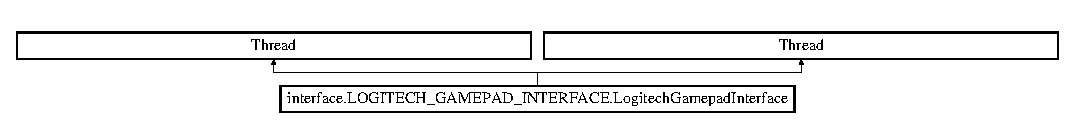
\includegraphics[height=0.640732cm]{classinterface_1_1LOGITECH__GAMEPAD__INTERFACE_1_1LogitechGamepadInterface}
\end{center}
\end{figure}
\subsection*{Public Member Functions}
\begin{DoxyCompactItemize}
\item 
def \hyperlink{classinterface_1_1LOGITECH__GAMEPAD__INTERFACE_1_1LogitechGamepadInterface_ae9cbbecadf735d90cf9834b4df772d2d}{\+\_\+\+\_\+init\+\_\+\+\_\+}
\item 
def \hyperlink{classinterface_1_1LOGITECH__GAMEPAD__INTERFACE_1_1LogitechGamepadInterface_a759473f1f4a54af72dabd5dcfa3f5d3b}{run}
\item 
def \hyperlink{classinterface_1_1LOGITECH__GAMEPAD__INTERFACE_1_1LogitechGamepadInterface_ae9cbbecadf735d90cf9834b4df772d2d}{\+\_\+\+\_\+init\+\_\+\+\_\+}
\item 
def \hyperlink{classinterface_1_1LOGITECH__GAMEPAD__INTERFACE_1_1LogitechGamepadInterface_a759473f1f4a54af72dabd5dcfa3f5d3b}{run}
\item 
def \hyperlink{classinterface_1_1LOGITECH__GAMEPAD__INTERFACE_1_1LogitechGamepadInterface_ae9cbbecadf735d90cf9834b4df772d2d}{\+\_\+\+\_\+init\+\_\+\+\_\+}
\item 
def \hyperlink{classinterface_1_1LOGITECH__GAMEPAD__INTERFACE_1_1LogitechGamepadInterface_a759473f1f4a54af72dabd5dcfa3f5d3b}{run}
\item 
def \hyperlink{classinterface_1_1LOGITECH__GAMEPAD__INTERFACE_1_1LogitechGamepadInterface_ae9cbbecadf735d90cf9834b4df772d2d}{\+\_\+\+\_\+init\+\_\+\+\_\+}
\item 
def \hyperlink{classinterface_1_1LOGITECH__GAMEPAD__INTERFACE_1_1LogitechGamepadInterface_a759473f1f4a54af72dabd5dcfa3f5d3b}{run}
\end{DoxyCompactItemize}
\subsection*{Public Attributes}
\begin{DoxyCompactItemize}
\item 
\hyperlink{classinterface_1_1LOGITECH__GAMEPAD__INTERFACE_1_1LogitechGamepadInterface_aa4c3375b698d7fdf478ceac2444ec437}{is\+Running}
\item 
\hyperlink{classinterface_1_1LOGITECH__GAMEPAD__INTERFACE_1_1LogitechGamepadInterface_afe919de9303d9c9c6f60e8b8db0755dd}{num}
\item 
\hyperlink{classinterface_1_1LOGITECH__GAMEPAD__INTERFACE_1_1LogitechGamepadInterface_a1ef8059ab625cac977f6a17662f5c0d9}{parent}
\item 
\hyperlink{classinterface_1_1LOGITECH__GAMEPAD__INTERFACE_1_1LogitechGamepadInterface_a35a43bbcfe3d9aab28bf43e147a5384c}{model}
\end{DoxyCompactItemize}


\subsection{Constructor \& Destructor Documentation}
\hypertarget{classinterface_1_1LOGITECH__GAMEPAD__INTERFACE_1_1LogitechGamepadInterface_ae9cbbecadf735d90cf9834b4df772d2d}{}\index{interface\+::\+L\+O\+G\+I\+T\+E\+C\+H\+\_\+\+G\+A\+M\+E\+P\+A\+D\+\_\+\+I\+N\+T\+E\+R\+F\+A\+C\+E\+::\+Logitech\+Gamepad\+Interface@{interface\+::\+L\+O\+G\+I\+T\+E\+C\+H\+\_\+\+G\+A\+M\+E\+P\+A\+D\+\_\+\+I\+N\+T\+E\+R\+F\+A\+C\+E\+::\+Logitech\+Gamepad\+Interface}!\+\_\+\+\_\+init\+\_\+\+\_\+@{\+\_\+\+\_\+init\+\_\+\+\_\+}}
\index{\+\_\+\+\_\+init\+\_\+\+\_\+@{\+\_\+\+\_\+init\+\_\+\+\_\+}!interface\+::\+L\+O\+G\+I\+T\+E\+C\+H\+\_\+\+G\+A\+M\+E\+P\+A\+D\+\_\+\+I\+N\+T\+E\+R\+F\+A\+C\+E\+::\+Logitech\+Gamepad\+Interface@{interface\+::\+L\+O\+G\+I\+T\+E\+C\+H\+\_\+\+G\+A\+M\+E\+P\+A\+D\+\_\+\+I\+N\+T\+E\+R\+F\+A\+C\+E\+::\+Logitech\+Gamepad\+Interface}}
\subsubsection[{\+\_\+\+\_\+init\+\_\+\+\_\+}]{\setlength{\rightskip}{0pt plus 5cm}def interface.\+L\+O\+G\+I\+T\+E\+C\+H\+\_\+\+G\+A\+M\+E\+P\+A\+D\+\_\+\+I\+N\+T\+E\+R\+F\+A\+C\+E.\+Logitech\+Gamepad\+Interface.\+\_\+\+\_\+init\+\_\+\+\_\+ (
\begin{DoxyParamCaption}
\item[{}]{self}
\end{DoxyParamCaption}
)}\label{classinterface_1_1LOGITECH__GAMEPAD__INTERFACE_1_1LogitechGamepadInterface_ae9cbbecadf735d90cf9834b4df772d2d}
\hypertarget{classinterface_1_1LOGITECH__GAMEPAD__INTERFACE_1_1LogitechGamepadInterface_ae9cbbecadf735d90cf9834b4df772d2d}{}\index{interface\+::\+L\+O\+G\+I\+T\+E\+C\+H\+\_\+\+G\+A\+M\+E\+P\+A\+D\+\_\+\+I\+N\+T\+E\+R\+F\+A\+C\+E\+::\+Logitech\+Gamepad\+Interface@{interface\+::\+L\+O\+G\+I\+T\+E\+C\+H\+\_\+\+G\+A\+M\+E\+P\+A\+D\+\_\+\+I\+N\+T\+E\+R\+F\+A\+C\+E\+::\+Logitech\+Gamepad\+Interface}!\+\_\+\+\_\+init\+\_\+\+\_\+@{\+\_\+\+\_\+init\+\_\+\+\_\+}}
\index{\+\_\+\+\_\+init\+\_\+\+\_\+@{\+\_\+\+\_\+init\+\_\+\+\_\+}!interface\+::\+L\+O\+G\+I\+T\+E\+C\+H\+\_\+\+G\+A\+M\+E\+P\+A\+D\+\_\+\+I\+N\+T\+E\+R\+F\+A\+C\+E\+::\+Logitech\+Gamepad\+Interface@{interface\+::\+L\+O\+G\+I\+T\+E\+C\+H\+\_\+\+G\+A\+M\+E\+P\+A\+D\+\_\+\+I\+N\+T\+E\+R\+F\+A\+C\+E\+::\+Logitech\+Gamepad\+Interface}}
\subsubsection[{\+\_\+\+\_\+init\+\_\+\+\_\+}]{\setlength{\rightskip}{0pt plus 5cm}def interface.\+L\+O\+G\+I\+T\+E\+C\+H\+\_\+\+G\+A\+M\+E\+P\+A\+D\+\_\+\+I\+N\+T\+E\+R\+F\+A\+C\+E.\+Logitech\+Gamepad\+Interface.\+\_\+\+\_\+init\+\_\+\+\_\+ (
\begin{DoxyParamCaption}
\item[{}]{self}
\end{DoxyParamCaption}
)}\label{classinterface_1_1LOGITECH__GAMEPAD__INTERFACE_1_1LogitechGamepadInterface_ae9cbbecadf735d90cf9834b4df772d2d}
\hypertarget{classinterface_1_1LOGITECH__GAMEPAD__INTERFACE_1_1LogitechGamepadInterface_ae9cbbecadf735d90cf9834b4df772d2d}{}\index{interface\+::\+L\+O\+G\+I\+T\+E\+C\+H\+\_\+\+G\+A\+M\+E\+P\+A\+D\+\_\+\+I\+N\+T\+E\+R\+F\+A\+C\+E\+::\+Logitech\+Gamepad\+Interface@{interface\+::\+L\+O\+G\+I\+T\+E\+C\+H\+\_\+\+G\+A\+M\+E\+P\+A\+D\+\_\+\+I\+N\+T\+E\+R\+F\+A\+C\+E\+::\+Logitech\+Gamepad\+Interface}!\+\_\+\+\_\+init\+\_\+\+\_\+@{\+\_\+\+\_\+init\+\_\+\+\_\+}}
\index{\+\_\+\+\_\+init\+\_\+\+\_\+@{\+\_\+\+\_\+init\+\_\+\+\_\+}!interface\+::\+L\+O\+G\+I\+T\+E\+C\+H\+\_\+\+G\+A\+M\+E\+P\+A\+D\+\_\+\+I\+N\+T\+E\+R\+F\+A\+C\+E\+::\+Logitech\+Gamepad\+Interface@{interface\+::\+L\+O\+G\+I\+T\+E\+C\+H\+\_\+\+G\+A\+M\+E\+P\+A\+D\+\_\+\+I\+N\+T\+E\+R\+F\+A\+C\+E\+::\+Logitech\+Gamepad\+Interface}}
\subsubsection[{\+\_\+\+\_\+init\+\_\+\+\_\+}]{\setlength{\rightskip}{0pt plus 5cm}def interface.\+L\+O\+G\+I\+T\+E\+C\+H\+\_\+\+G\+A\+M\+E\+P\+A\+D\+\_\+\+I\+N\+T\+E\+R\+F\+A\+C\+E.\+Logitech\+Gamepad\+Interface.\+\_\+\+\_\+init\+\_\+\+\_\+ (
\begin{DoxyParamCaption}
\item[{}]{self}
\end{DoxyParamCaption}
)}\label{classinterface_1_1LOGITECH__GAMEPAD__INTERFACE_1_1LogitechGamepadInterface_ae9cbbecadf735d90cf9834b4df772d2d}
\hypertarget{classinterface_1_1LOGITECH__GAMEPAD__INTERFACE_1_1LogitechGamepadInterface_ae9cbbecadf735d90cf9834b4df772d2d}{}\index{interface\+::\+L\+O\+G\+I\+T\+E\+C\+H\+\_\+\+G\+A\+M\+E\+P\+A\+D\+\_\+\+I\+N\+T\+E\+R\+F\+A\+C\+E\+::\+Logitech\+Gamepad\+Interface@{interface\+::\+L\+O\+G\+I\+T\+E\+C\+H\+\_\+\+G\+A\+M\+E\+P\+A\+D\+\_\+\+I\+N\+T\+E\+R\+F\+A\+C\+E\+::\+Logitech\+Gamepad\+Interface}!\+\_\+\+\_\+init\+\_\+\+\_\+@{\+\_\+\+\_\+init\+\_\+\+\_\+}}
\index{\+\_\+\+\_\+init\+\_\+\+\_\+@{\+\_\+\+\_\+init\+\_\+\+\_\+}!interface\+::\+L\+O\+G\+I\+T\+E\+C\+H\+\_\+\+G\+A\+M\+E\+P\+A\+D\+\_\+\+I\+N\+T\+E\+R\+F\+A\+C\+E\+::\+Logitech\+Gamepad\+Interface@{interface\+::\+L\+O\+G\+I\+T\+E\+C\+H\+\_\+\+G\+A\+M\+E\+P\+A\+D\+\_\+\+I\+N\+T\+E\+R\+F\+A\+C\+E\+::\+Logitech\+Gamepad\+Interface}}
\subsubsection[{\+\_\+\+\_\+init\+\_\+\+\_\+}]{\setlength{\rightskip}{0pt plus 5cm}def interface.\+L\+O\+G\+I\+T\+E\+C\+H\+\_\+\+G\+A\+M\+E\+P\+A\+D\+\_\+\+I\+N\+T\+E\+R\+F\+A\+C\+E.\+Logitech\+Gamepad\+Interface.\+\_\+\+\_\+init\+\_\+\+\_\+ (
\begin{DoxyParamCaption}
\item[{}]{self}
\end{DoxyParamCaption}
)}\label{classinterface_1_1LOGITECH__GAMEPAD__INTERFACE_1_1LogitechGamepadInterface_ae9cbbecadf735d90cf9834b4df772d2d}


\subsection{Member Function Documentation}
\hypertarget{classinterface_1_1LOGITECH__GAMEPAD__INTERFACE_1_1LogitechGamepadInterface_a759473f1f4a54af72dabd5dcfa3f5d3b}{}\index{interface\+::\+L\+O\+G\+I\+T\+E\+C\+H\+\_\+\+G\+A\+M\+E\+P\+A\+D\+\_\+\+I\+N\+T\+E\+R\+F\+A\+C\+E\+::\+Logitech\+Gamepad\+Interface@{interface\+::\+L\+O\+G\+I\+T\+E\+C\+H\+\_\+\+G\+A\+M\+E\+P\+A\+D\+\_\+\+I\+N\+T\+E\+R\+F\+A\+C\+E\+::\+Logitech\+Gamepad\+Interface}!run@{run}}
\index{run@{run}!interface\+::\+L\+O\+G\+I\+T\+E\+C\+H\+\_\+\+G\+A\+M\+E\+P\+A\+D\+\_\+\+I\+N\+T\+E\+R\+F\+A\+C\+E\+::\+Logitech\+Gamepad\+Interface@{interface\+::\+L\+O\+G\+I\+T\+E\+C\+H\+\_\+\+G\+A\+M\+E\+P\+A\+D\+\_\+\+I\+N\+T\+E\+R\+F\+A\+C\+E\+::\+Logitech\+Gamepad\+Interface}}
\subsubsection[{run}]{\setlength{\rightskip}{0pt plus 5cm}def interface.\+L\+O\+G\+I\+T\+E\+C\+H\+\_\+\+G\+A\+M\+E\+P\+A\+D\+\_\+\+I\+N\+T\+E\+R\+F\+A\+C\+E.\+Logitech\+Gamepad\+Interface.\+run (
\begin{DoxyParamCaption}
\item[{}]{self}
\end{DoxyParamCaption}
)}\label{classinterface_1_1LOGITECH__GAMEPAD__INTERFACE_1_1LogitechGamepadInterface_a759473f1f4a54af72dabd5dcfa3f5d3b}
\hypertarget{classinterface_1_1LOGITECH__GAMEPAD__INTERFACE_1_1LogitechGamepadInterface_a759473f1f4a54af72dabd5dcfa3f5d3b}{}\index{interface\+::\+L\+O\+G\+I\+T\+E\+C\+H\+\_\+\+G\+A\+M\+E\+P\+A\+D\+\_\+\+I\+N\+T\+E\+R\+F\+A\+C\+E\+::\+Logitech\+Gamepad\+Interface@{interface\+::\+L\+O\+G\+I\+T\+E\+C\+H\+\_\+\+G\+A\+M\+E\+P\+A\+D\+\_\+\+I\+N\+T\+E\+R\+F\+A\+C\+E\+::\+Logitech\+Gamepad\+Interface}!run@{run}}
\index{run@{run}!interface\+::\+L\+O\+G\+I\+T\+E\+C\+H\+\_\+\+G\+A\+M\+E\+P\+A\+D\+\_\+\+I\+N\+T\+E\+R\+F\+A\+C\+E\+::\+Logitech\+Gamepad\+Interface@{interface\+::\+L\+O\+G\+I\+T\+E\+C\+H\+\_\+\+G\+A\+M\+E\+P\+A\+D\+\_\+\+I\+N\+T\+E\+R\+F\+A\+C\+E\+::\+Logitech\+Gamepad\+Interface}}
\subsubsection[{run}]{\setlength{\rightskip}{0pt plus 5cm}def interface.\+L\+O\+G\+I\+T\+E\+C\+H\+\_\+\+G\+A\+M\+E\+P\+A\+D\+\_\+\+I\+N\+T\+E\+R\+F\+A\+C\+E.\+Logitech\+Gamepad\+Interface.\+run (
\begin{DoxyParamCaption}
\item[{}]{self}
\end{DoxyParamCaption}
)}\label{classinterface_1_1LOGITECH__GAMEPAD__INTERFACE_1_1LogitechGamepadInterface_a759473f1f4a54af72dabd5dcfa3f5d3b}
\hypertarget{classinterface_1_1LOGITECH__GAMEPAD__INTERFACE_1_1LogitechGamepadInterface_a759473f1f4a54af72dabd5dcfa3f5d3b}{}\index{interface\+::\+L\+O\+G\+I\+T\+E\+C\+H\+\_\+\+G\+A\+M\+E\+P\+A\+D\+\_\+\+I\+N\+T\+E\+R\+F\+A\+C\+E\+::\+Logitech\+Gamepad\+Interface@{interface\+::\+L\+O\+G\+I\+T\+E\+C\+H\+\_\+\+G\+A\+M\+E\+P\+A\+D\+\_\+\+I\+N\+T\+E\+R\+F\+A\+C\+E\+::\+Logitech\+Gamepad\+Interface}!run@{run}}
\index{run@{run}!interface\+::\+L\+O\+G\+I\+T\+E\+C\+H\+\_\+\+G\+A\+M\+E\+P\+A\+D\+\_\+\+I\+N\+T\+E\+R\+F\+A\+C\+E\+::\+Logitech\+Gamepad\+Interface@{interface\+::\+L\+O\+G\+I\+T\+E\+C\+H\+\_\+\+G\+A\+M\+E\+P\+A\+D\+\_\+\+I\+N\+T\+E\+R\+F\+A\+C\+E\+::\+Logitech\+Gamepad\+Interface}}
\subsubsection[{run}]{\setlength{\rightskip}{0pt plus 5cm}def interface.\+L\+O\+G\+I\+T\+E\+C\+H\+\_\+\+G\+A\+M\+E\+P\+A\+D\+\_\+\+I\+N\+T\+E\+R\+F\+A\+C\+E.\+Logitech\+Gamepad\+Interface.\+run (
\begin{DoxyParamCaption}
\item[{}]{self}
\end{DoxyParamCaption}
)}\label{classinterface_1_1LOGITECH__GAMEPAD__INTERFACE_1_1LogitechGamepadInterface_a759473f1f4a54af72dabd5dcfa3f5d3b}
\hypertarget{classinterface_1_1LOGITECH__GAMEPAD__INTERFACE_1_1LogitechGamepadInterface_a759473f1f4a54af72dabd5dcfa3f5d3b}{}\index{interface\+::\+L\+O\+G\+I\+T\+E\+C\+H\+\_\+\+G\+A\+M\+E\+P\+A\+D\+\_\+\+I\+N\+T\+E\+R\+F\+A\+C\+E\+::\+Logitech\+Gamepad\+Interface@{interface\+::\+L\+O\+G\+I\+T\+E\+C\+H\+\_\+\+G\+A\+M\+E\+P\+A\+D\+\_\+\+I\+N\+T\+E\+R\+F\+A\+C\+E\+::\+Logitech\+Gamepad\+Interface}!run@{run}}
\index{run@{run}!interface\+::\+L\+O\+G\+I\+T\+E\+C\+H\+\_\+\+G\+A\+M\+E\+P\+A\+D\+\_\+\+I\+N\+T\+E\+R\+F\+A\+C\+E\+::\+Logitech\+Gamepad\+Interface@{interface\+::\+L\+O\+G\+I\+T\+E\+C\+H\+\_\+\+G\+A\+M\+E\+P\+A\+D\+\_\+\+I\+N\+T\+E\+R\+F\+A\+C\+E\+::\+Logitech\+Gamepad\+Interface}}
\subsubsection[{run}]{\setlength{\rightskip}{0pt plus 5cm}def interface.\+L\+O\+G\+I\+T\+E\+C\+H\+\_\+\+G\+A\+M\+E\+P\+A\+D\+\_\+\+I\+N\+T\+E\+R\+F\+A\+C\+E.\+Logitech\+Gamepad\+Interface.\+run (
\begin{DoxyParamCaption}
\item[{}]{self}
\end{DoxyParamCaption}
)}\label{classinterface_1_1LOGITECH__GAMEPAD__INTERFACE_1_1LogitechGamepadInterface_a759473f1f4a54af72dabd5dcfa3f5d3b}


\subsection{Member Data Documentation}
\hypertarget{classinterface_1_1LOGITECH__GAMEPAD__INTERFACE_1_1LogitechGamepadInterface_aa4c3375b698d7fdf478ceac2444ec437}{}\index{interface\+::\+L\+O\+G\+I\+T\+E\+C\+H\+\_\+\+G\+A\+M\+E\+P\+A\+D\+\_\+\+I\+N\+T\+E\+R\+F\+A\+C\+E\+::\+Logitech\+Gamepad\+Interface@{interface\+::\+L\+O\+G\+I\+T\+E\+C\+H\+\_\+\+G\+A\+M\+E\+P\+A\+D\+\_\+\+I\+N\+T\+E\+R\+F\+A\+C\+E\+::\+Logitech\+Gamepad\+Interface}!is\+Running@{is\+Running}}
\index{is\+Running@{is\+Running}!interface\+::\+L\+O\+G\+I\+T\+E\+C\+H\+\_\+\+G\+A\+M\+E\+P\+A\+D\+\_\+\+I\+N\+T\+E\+R\+F\+A\+C\+E\+::\+Logitech\+Gamepad\+Interface@{interface\+::\+L\+O\+G\+I\+T\+E\+C\+H\+\_\+\+G\+A\+M\+E\+P\+A\+D\+\_\+\+I\+N\+T\+E\+R\+F\+A\+C\+E\+::\+Logitech\+Gamepad\+Interface}}
\subsubsection[{is\+Running}]{\setlength{\rightskip}{0pt plus 5cm}interface.\+L\+O\+G\+I\+T\+E\+C\+H\+\_\+\+G\+A\+M\+E\+P\+A\+D\+\_\+\+I\+N\+T\+E\+R\+F\+A\+C\+E.\+Logitech\+Gamepad\+Interface.\+is\+Running}\label{classinterface_1_1LOGITECH__GAMEPAD__INTERFACE_1_1LogitechGamepadInterface_aa4c3375b698d7fdf478ceac2444ec437}
\hypertarget{classinterface_1_1LOGITECH__GAMEPAD__INTERFACE_1_1LogitechGamepadInterface_a35a43bbcfe3d9aab28bf43e147a5384c}{}\index{interface\+::\+L\+O\+G\+I\+T\+E\+C\+H\+\_\+\+G\+A\+M\+E\+P\+A\+D\+\_\+\+I\+N\+T\+E\+R\+F\+A\+C\+E\+::\+Logitech\+Gamepad\+Interface@{interface\+::\+L\+O\+G\+I\+T\+E\+C\+H\+\_\+\+G\+A\+M\+E\+P\+A\+D\+\_\+\+I\+N\+T\+E\+R\+F\+A\+C\+E\+::\+Logitech\+Gamepad\+Interface}!model@{model}}
\index{model@{model}!interface\+::\+L\+O\+G\+I\+T\+E\+C\+H\+\_\+\+G\+A\+M\+E\+P\+A\+D\+\_\+\+I\+N\+T\+E\+R\+F\+A\+C\+E\+::\+Logitech\+Gamepad\+Interface@{interface\+::\+L\+O\+G\+I\+T\+E\+C\+H\+\_\+\+G\+A\+M\+E\+P\+A\+D\+\_\+\+I\+N\+T\+E\+R\+F\+A\+C\+E\+::\+Logitech\+Gamepad\+Interface}}
\subsubsection[{model}]{\setlength{\rightskip}{0pt plus 5cm}interface.\+L\+O\+G\+I\+T\+E\+C\+H\+\_\+\+G\+A\+M\+E\+P\+A\+D\+\_\+\+I\+N\+T\+E\+R\+F\+A\+C\+E.\+Logitech\+Gamepad\+Interface.\+model}\label{classinterface_1_1LOGITECH__GAMEPAD__INTERFACE_1_1LogitechGamepadInterface_a35a43bbcfe3d9aab28bf43e147a5384c}
\hypertarget{classinterface_1_1LOGITECH__GAMEPAD__INTERFACE_1_1LogitechGamepadInterface_afe919de9303d9c9c6f60e8b8db0755dd}{}\index{interface\+::\+L\+O\+G\+I\+T\+E\+C\+H\+\_\+\+G\+A\+M\+E\+P\+A\+D\+\_\+\+I\+N\+T\+E\+R\+F\+A\+C\+E\+::\+Logitech\+Gamepad\+Interface@{interface\+::\+L\+O\+G\+I\+T\+E\+C\+H\+\_\+\+G\+A\+M\+E\+P\+A\+D\+\_\+\+I\+N\+T\+E\+R\+F\+A\+C\+E\+::\+Logitech\+Gamepad\+Interface}!num@{num}}
\index{num@{num}!interface\+::\+L\+O\+G\+I\+T\+E\+C\+H\+\_\+\+G\+A\+M\+E\+P\+A\+D\+\_\+\+I\+N\+T\+E\+R\+F\+A\+C\+E\+::\+Logitech\+Gamepad\+Interface@{interface\+::\+L\+O\+G\+I\+T\+E\+C\+H\+\_\+\+G\+A\+M\+E\+P\+A\+D\+\_\+\+I\+N\+T\+E\+R\+F\+A\+C\+E\+::\+Logitech\+Gamepad\+Interface}}
\subsubsection[{num}]{\setlength{\rightskip}{0pt plus 5cm}interface.\+L\+O\+G\+I\+T\+E\+C\+H\+\_\+\+G\+A\+M\+E\+P\+A\+D\+\_\+\+I\+N\+T\+E\+R\+F\+A\+C\+E.\+Logitech\+Gamepad\+Interface.\+num}\label{classinterface_1_1LOGITECH__GAMEPAD__INTERFACE_1_1LogitechGamepadInterface_afe919de9303d9c9c6f60e8b8db0755dd}
\hypertarget{classinterface_1_1LOGITECH__GAMEPAD__INTERFACE_1_1LogitechGamepadInterface_a1ef8059ab625cac977f6a17662f5c0d9}{}\index{interface\+::\+L\+O\+G\+I\+T\+E\+C\+H\+\_\+\+G\+A\+M\+E\+P\+A\+D\+\_\+\+I\+N\+T\+E\+R\+F\+A\+C\+E\+::\+Logitech\+Gamepad\+Interface@{interface\+::\+L\+O\+G\+I\+T\+E\+C\+H\+\_\+\+G\+A\+M\+E\+P\+A\+D\+\_\+\+I\+N\+T\+E\+R\+F\+A\+C\+E\+::\+Logitech\+Gamepad\+Interface}!parent@{parent}}
\index{parent@{parent}!interface\+::\+L\+O\+G\+I\+T\+E\+C\+H\+\_\+\+G\+A\+M\+E\+P\+A\+D\+\_\+\+I\+N\+T\+E\+R\+F\+A\+C\+E\+::\+Logitech\+Gamepad\+Interface@{interface\+::\+L\+O\+G\+I\+T\+E\+C\+H\+\_\+\+G\+A\+M\+E\+P\+A\+D\+\_\+\+I\+N\+T\+E\+R\+F\+A\+C\+E\+::\+Logitech\+Gamepad\+Interface}}
\subsubsection[{parent}]{\setlength{\rightskip}{0pt plus 5cm}interface.\+L\+O\+G\+I\+T\+E\+C\+H\+\_\+\+G\+A\+M\+E\+P\+A\+D\+\_\+\+I\+N\+T\+E\+R\+F\+A\+C\+E.\+Logitech\+Gamepad\+Interface.\+parent}\label{classinterface_1_1LOGITECH__GAMEPAD__INTERFACE_1_1LogitechGamepadInterface_a1ef8059ab625cac977f6a17662f5c0d9}


The documentation for this class was generated from the following file\+:\begin{DoxyCompactItemize}
\item 
build/lib.\+linux-\/x86\+\_\+64-\/2.\+7/interface/\hyperlink{build_2lib_8linux-x86__64-2_87_2interface_2LOGITECH__GAMEPAD__INTERFACE_8py}{L\+O\+G\+I\+T\+E\+C\+H\+\_\+\+G\+A\+M\+E\+P\+A\+D\+\_\+\+I\+N\+T\+E\+R\+F\+A\+C\+E.\+py}\end{DoxyCompactItemize}

\hypertarget{classmodel_1_1LOGITECH__GAMEPAD__MODEL_1_1LogitechGamepadModel}{}\section{model.\+L\+O\+G\+I\+T\+E\+C\+H\+\_\+\+G\+A\+M\+E\+P\+A\+D\+\_\+\+M\+O\+D\+E\+L.\+Logitech\+Gamepad\+Model Class Reference}
\label{classmodel_1_1LOGITECH__GAMEPAD__MODEL_1_1LogitechGamepadModel}\index{model.\+L\+O\+G\+I\+T\+E\+C\+H\+\_\+\+G\+A\+M\+E\+P\+A\+D\+\_\+\+M\+O\+D\+E\+L.\+Logitech\+Gamepad\+Model@{model.\+L\+O\+G\+I\+T\+E\+C\+H\+\_\+\+G\+A\+M\+E\+P\+A\+D\+\_\+\+M\+O\+D\+E\+L.\+Logitech\+Gamepad\+Model}}
\subsection*{Public Member Functions}
\begin{DoxyCompactItemize}
\item 
def \hyperlink{classmodel_1_1LOGITECH__GAMEPAD__MODEL_1_1LogitechGamepadModel_a78c8eb4ec8b24bb9b7b3b5f8b89b1ae4}{\+\_\+\+\_\+init\+\_\+\+\_\+}
\item 
def \hyperlink{classmodel_1_1LOGITECH__GAMEPAD__MODEL_1_1LogitechGamepadModel_a78c8eb4ec8b24bb9b7b3b5f8b89b1ae4}{\+\_\+\+\_\+init\+\_\+\+\_\+}
\end{DoxyCompactItemize}
\subsection*{Public Attributes}
\begin{DoxyCompactItemize}
\item 
\hyperlink{classmodel_1_1LOGITECH__GAMEPAD__MODEL_1_1LogitechGamepadModel_aca968abc43721d36876b94f20d9710d4}{name}
\item 
\hyperlink{classmodel_1_1LOGITECH__GAMEPAD__MODEL_1_1LogitechGamepadModel_ae06162ea90b5693d17eafe7b409befbf}{axis\+L\+X}
\item 
\hyperlink{classmodel_1_1LOGITECH__GAMEPAD__MODEL_1_1LogitechGamepadModel_a31e503a0ce36f109abf7f77d7947fd19}{axis\+L\+Y}
\item 
\hyperlink{classmodel_1_1LOGITECH__GAMEPAD__MODEL_1_1LogitechGamepadModel_ab17ce1369de5fe967d8b8c73878fbd52}{axis\+R\+X}
\item 
\hyperlink{classmodel_1_1LOGITECH__GAMEPAD__MODEL_1_1LogitechGamepadModel_ade6496f07c4f4262a30d7c2c28615023}{axis\+R\+Y}
\item 
\hyperlink{classmodel_1_1LOGITECH__GAMEPAD__MODEL_1_1LogitechGamepadModel_aedc880781d845d342dbb2bd108eaba01}{button\+A}
\item 
\hyperlink{classmodel_1_1LOGITECH__GAMEPAD__MODEL_1_1LogitechGamepadModel_aaa57eb747fdecfcec0ead5b0f44e419d}{button\+B}
\item 
\hyperlink{classmodel_1_1LOGITECH__GAMEPAD__MODEL_1_1LogitechGamepadModel_a670e7ef57a4bf689e482638da67c51a6}{button\+X}
\item 
\hyperlink{classmodel_1_1LOGITECH__GAMEPAD__MODEL_1_1LogitechGamepadModel_a72856dfccd01178bf48d32817812950f}{button\+Y}
\item 
\hyperlink{classmodel_1_1LOGITECH__GAMEPAD__MODEL_1_1LogitechGamepadModel_afe48154427bd2d13420fa732be1e3768}{button\+L\+B}
\item 
\hyperlink{classmodel_1_1LOGITECH__GAMEPAD__MODEL_1_1LogitechGamepadModel_a957467219bf265c86235c336a3ede697}{button\+R\+B}
\item 
\hyperlink{classmodel_1_1LOGITECH__GAMEPAD__MODEL_1_1LogitechGamepadModel_adeac4ea09334e4fefe9ee678a765e3b0}{button\+L\+T}
\item 
\hyperlink{classmodel_1_1LOGITECH__GAMEPAD__MODEL_1_1LogitechGamepadModel_a86da339acfa5067037601408a5d49c24}{button\+R\+T}
\item 
\hyperlink{classmodel_1_1LOGITECH__GAMEPAD__MODEL_1_1LogitechGamepadModel_a69935e9b8ea79f561606c868151c0326}{button\+Back}
\item 
\hyperlink{classmodel_1_1LOGITECH__GAMEPAD__MODEL_1_1LogitechGamepadModel_ab794dea015179ef967b0a7158155f875}{button\+Start}
\item 
\hyperlink{classmodel_1_1LOGITECH__GAMEPAD__MODEL_1_1LogitechGamepadModel_a4d4a5ae309e7d6442204e1206f2bf390}{d\+Pad\+Left}
\item 
\hyperlink{classmodel_1_1LOGITECH__GAMEPAD__MODEL_1_1LogitechGamepadModel_a82934ed6d614ab974ab4ca2fe1488933}{d\+Pad\+Right}
\item 
\hyperlink{classmodel_1_1LOGITECH__GAMEPAD__MODEL_1_1LogitechGamepadModel_a260b07781293ab823c5f1963fcd40d03}{d\+Pad\+Up}
\item 
\hyperlink{classmodel_1_1LOGITECH__GAMEPAD__MODEL_1_1LogitechGamepadModel_a63f6d8dc05a0884eaebc6d2a1f8b62f0}{d\+Pad\+Down}
\item 
\hyperlink{classmodel_1_1LOGITECH__GAMEPAD__MODEL_1_1LogitechGamepadModel_a77eb2ddae3b91d8da8845214893c118d}{gamepad}
\item 
\hyperlink{classmodel_1_1LOGITECH__GAMEPAD__MODEL_1_1LogitechGamepadModel_a6c98021d546456249760f86386c7d406}{is\+Running}
\end{DoxyCompactItemize}


\subsection{Constructor \& Destructor Documentation}
\hypertarget{classmodel_1_1LOGITECH__GAMEPAD__MODEL_1_1LogitechGamepadModel_a78c8eb4ec8b24bb9b7b3b5f8b89b1ae4}{}\index{model\+::\+L\+O\+G\+I\+T\+E\+C\+H\+\_\+\+G\+A\+M\+E\+P\+A\+D\+\_\+\+M\+O\+D\+E\+L\+::\+Logitech\+Gamepad\+Model@{model\+::\+L\+O\+G\+I\+T\+E\+C\+H\+\_\+\+G\+A\+M\+E\+P\+A\+D\+\_\+\+M\+O\+D\+E\+L\+::\+Logitech\+Gamepad\+Model}!\+\_\+\+\_\+init\+\_\+\+\_\+@{\+\_\+\+\_\+init\+\_\+\+\_\+}}
\index{\+\_\+\+\_\+init\+\_\+\+\_\+@{\+\_\+\+\_\+init\+\_\+\+\_\+}!model\+::\+L\+O\+G\+I\+T\+E\+C\+H\+\_\+\+G\+A\+M\+E\+P\+A\+D\+\_\+\+M\+O\+D\+E\+L\+::\+Logitech\+Gamepad\+Model@{model\+::\+L\+O\+G\+I\+T\+E\+C\+H\+\_\+\+G\+A\+M\+E\+P\+A\+D\+\_\+\+M\+O\+D\+E\+L\+::\+Logitech\+Gamepad\+Model}}
\subsubsection[{\+\_\+\+\_\+init\+\_\+\+\_\+}]{\setlength{\rightskip}{0pt plus 5cm}def model.\+L\+O\+G\+I\+T\+E\+C\+H\+\_\+\+G\+A\+M\+E\+P\+A\+D\+\_\+\+M\+O\+D\+E\+L.\+Logitech\+Gamepad\+Model.\+\_\+\+\_\+init\+\_\+\+\_\+ (
\begin{DoxyParamCaption}
\item[{}]{self}
\end{DoxyParamCaption}
)}\label{classmodel_1_1LOGITECH__GAMEPAD__MODEL_1_1LogitechGamepadModel_a78c8eb4ec8b24bb9b7b3b5f8b89b1ae4}
\hypertarget{classmodel_1_1LOGITECH__GAMEPAD__MODEL_1_1LogitechGamepadModel_a78c8eb4ec8b24bb9b7b3b5f8b89b1ae4}{}\index{model\+::\+L\+O\+G\+I\+T\+E\+C\+H\+\_\+\+G\+A\+M\+E\+P\+A\+D\+\_\+\+M\+O\+D\+E\+L\+::\+Logitech\+Gamepad\+Model@{model\+::\+L\+O\+G\+I\+T\+E\+C\+H\+\_\+\+G\+A\+M\+E\+P\+A\+D\+\_\+\+M\+O\+D\+E\+L\+::\+Logitech\+Gamepad\+Model}!\+\_\+\+\_\+init\+\_\+\+\_\+@{\+\_\+\+\_\+init\+\_\+\+\_\+}}
\index{\+\_\+\+\_\+init\+\_\+\+\_\+@{\+\_\+\+\_\+init\+\_\+\+\_\+}!model\+::\+L\+O\+G\+I\+T\+E\+C\+H\+\_\+\+G\+A\+M\+E\+P\+A\+D\+\_\+\+M\+O\+D\+E\+L\+::\+Logitech\+Gamepad\+Model@{model\+::\+L\+O\+G\+I\+T\+E\+C\+H\+\_\+\+G\+A\+M\+E\+P\+A\+D\+\_\+\+M\+O\+D\+E\+L\+::\+Logitech\+Gamepad\+Model}}
\subsubsection[{\+\_\+\+\_\+init\+\_\+\+\_\+}]{\setlength{\rightskip}{0pt plus 5cm}def model.\+L\+O\+G\+I\+T\+E\+C\+H\+\_\+\+G\+A\+M\+E\+P\+A\+D\+\_\+\+M\+O\+D\+E\+L.\+Logitech\+Gamepad\+Model.\+\_\+\+\_\+init\+\_\+\+\_\+ (
\begin{DoxyParamCaption}
\item[{}]{self}
\end{DoxyParamCaption}
)}\label{classmodel_1_1LOGITECH__GAMEPAD__MODEL_1_1LogitechGamepadModel_a78c8eb4ec8b24bb9b7b3b5f8b89b1ae4}


\subsection{Member Data Documentation}
\hypertarget{classmodel_1_1LOGITECH__GAMEPAD__MODEL_1_1LogitechGamepadModel_ae06162ea90b5693d17eafe7b409befbf}{}\index{model\+::\+L\+O\+G\+I\+T\+E\+C\+H\+\_\+\+G\+A\+M\+E\+P\+A\+D\+\_\+\+M\+O\+D\+E\+L\+::\+Logitech\+Gamepad\+Model@{model\+::\+L\+O\+G\+I\+T\+E\+C\+H\+\_\+\+G\+A\+M\+E\+P\+A\+D\+\_\+\+M\+O\+D\+E\+L\+::\+Logitech\+Gamepad\+Model}!axis\+L\+X@{axis\+L\+X}}
\index{axis\+L\+X@{axis\+L\+X}!model\+::\+L\+O\+G\+I\+T\+E\+C\+H\+\_\+\+G\+A\+M\+E\+P\+A\+D\+\_\+\+M\+O\+D\+E\+L\+::\+Logitech\+Gamepad\+Model@{model\+::\+L\+O\+G\+I\+T\+E\+C\+H\+\_\+\+G\+A\+M\+E\+P\+A\+D\+\_\+\+M\+O\+D\+E\+L\+::\+Logitech\+Gamepad\+Model}}
\subsubsection[{axis\+L\+X}]{\setlength{\rightskip}{0pt plus 5cm}model.\+L\+O\+G\+I\+T\+E\+C\+H\+\_\+\+G\+A\+M\+E\+P\+A\+D\+\_\+\+M\+O\+D\+E\+L.\+Logitech\+Gamepad\+Model.\+axis\+L\+X}\label{classmodel_1_1LOGITECH__GAMEPAD__MODEL_1_1LogitechGamepadModel_ae06162ea90b5693d17eafe7b409befbf}
\hypertarget{classmodel_1_1LOGITECH__GAMEPAD__MODEL_1_1LogitechGamepadModel_a31e503a0ce36f109abf7f77d7947fd19}{}\index{model\+::\+L\+O\+G\+I\+T\+E\+C\+H\+\_\+\+G\+A\+M\+E\+P\+A\+D\+\_\+\+M\+O\+D\+E\+L\+::\+Logitech\+Gamepad\+Model@{model\+::\+L\+O\+G\+I\+T\+E\+C\+H\+\_\+\+G\+A\+M\+E\+P\+A\+D\+\_\+\+M\+O\+D\+E\+L\+::\+Logitech\+Gamepad\+Model}!axis\+L\+Y@{axis\+L\+Y}}
\index{axis\+L\+Y@{axis\+L\+Y}!model\+::\+L\+O\+G\+I\+T\+E\+C\+H\+\_\+\+G\+A\+M\+E\+P\+A\+D\+\_\+\+M\+O\+D\+E\+L\+::\+Logitech\+Gamepad\+Model@{model\+::\+L\+O\+G\+I\+T\+E\+C\+H\+\_\+\+G\+A\+M\+E\+P\+A\+D\+\_\+\+M\+O\+D\+E\+L\+::\+Logitech\+Gamepad\+Model}}
\subsubsection[{axis\+L\+Y}]{\setlength{\rightskip}{0pt plus 5cm}model.\+L\+O\+G\+I\+T\+E\+C\+H\+\_\+\+G\+A\+M\+E\+P\+A\+D\+\_\+\+M\+O\+D\+E\+L.\+Logitech\+Gamepad\+Model.\+axis\+L\+Y}\label{classmodel_1_1LOGITECH__GAMEPAD__MODEL_1_1LogitechGamepadModel_a31e503a0ce36f109abf7f77d7947fd19}
\hypertarget{classmodel_1_1LOGITECH__GAMEPAD__MODEL_1_1LogitechGamepadModel_ab17ce1369de5fe967d8b8c73878fbd52}{}\index{model\+::\+L\+O\+G\+I\+T\+E\+C\+H\+\_\+\+G\+A\+M\+E\+P\+A\+D\+\_\+\+M\+O\+D\+E\+L\+::\+Logitech\+Gamepad\+Model@{model\+::\+L\+O\+G\+I\+T\+E\+C\+H\+\_\+\+G\+A\+M\+E\+P\+A\+D\+\_\+\+M\+O\+D\+E\+L\+::\+Logitech\+Gamepad\+Model}!axis\+R\+X@{axis\+R\+X}}
\index{axis\+R\+X@{axis\+R\+X}!model\+::\+L\+O\+G\+I\+T\+E\+C\+H\+\_\+\+G\+A\+M\+E\+P\+A\+D\+\_\+\+M\+O\+D\+E\+L\+::\+Logitech\+Gamepad\+Model@{model\+::\+L\+O\+G\+I\+T\+E\+C\+H\+\_\+\+G\+A\+M\+E\+P\+A\+D\+\_\+\+M\+O\+D\+E\+L\+::\+Logitech\+Gamepad\+Model}}
\subsubsection[{axis\+R\+X}]{\setlength{\rightskip}{0pt plus 5cm}model.\+L\+O\+G\+I\+T\+E\+C\+H\+\_\+\+G\+A\+M\+E\+P\+A\+D\+\_\+\+M\+O\+D\+E\+L.\+Logitech\+Gamepad\+Model.\+axis\+R\+X}\label{classmodel_1_1LOGITECH__GAMEPAD__MODEL_1_1LogitechGamepadModel_ab17ce1369de5fe967d8b8c73878fbd52}
\hypertarget{classmodel_1_1LOGITECH__GAMEPAD__MODEL_1_1LogitechGamepadModel_ade6496f07c4f4262a30d7c2c28615023}{}\index{model\+::\+L\+O\+G\+I\+T\+E\+C\+H\+\_\+\+G\+A\+M\+E\+P\+A\+D\+\_\+\+M\+O\+D\+E\+L\+::\+Logitech\+Gamepad\+Model@{model\+::\+L\+O\+G\+I\+T\+E\+C\+H\+\_\+\+G\+A\+M\+E\+P\+A\+D\+\_\+\+M\+O\+D\+E\+L\+::\+Logitech\+Gamepad\+Model}!axis\+R\+Y@{axis\+R\+Y}}
\index{axis\+R\+Y@{axis\+R\+Y}!model\+::\+L\+O\+G\+I\+T\+E\+C\+H\+\_\+\+G\+A\+M\+E\+P\+A\+D\+\_\+\+M\+O\+D\+E\+L\+::\+Logitech\+Gamepad\+Model@{model\+::\+L\+O\+G\+I\+T\+E\+C\+H\+\_\+\+G\+A\+M\+E\+P\+A\+D\+\_\+\+M\+O\+D\+E\+L\+::\+Logitech\+Gamepad\+Model}}
\subsubsection[{axis\+R\+Y}]{\setlength{\rightskip}{0pt plus 5cm}model.\+L\+O\+G\+I\+T\+E\+C\+H\+\_\+\+G\+A\+M\+E\+P\+A\+D\+\_\+\+M\+O\+D\+E\+L.\+Logitech\+Gamepad\+Model.\+axis\+R\+Y}\label{classmodel_1_1LOGITECH__GAMEPAD__MODEL_1_1LogitechGamepadModel_ade6496f07c4f4262a30d7c2c28615023}
\hypertarget{classmodel_1_1LOGITECH__GAMEPAD__MODEL_1_1LogitechGamepadModel_aedc880781d845d342dbb2bd108eaba01}{}\index{model\+::\+L\+O\+G\+I\+T\+E\+C\+H\+\_\+\+G\+A\+M\+E\+P\+A\+D\+\_\+\+M\+O\+D\+E\+L\+::\+Logitech\+Gamepad\+Model@{model\+::\+L\+O\+G\+I\+T\+E\+C\+H\+\_\+\+G\+A\+M\+E\+P\+A\+D\+\_\+\+M\+O\+D\+E\+L\+::\+Logitech\+Gamepad\+Model}!button\+A@{button\+A}}
\index{button\+A@{button\+A}!model\+::\+L\+O\+G\+I\+T\+E\+C\+H\+\_\+\+G\+A\+M\+E\+P\+A\+D\+\_\+\+M\+O\+D\+E\+L\+::\+Logitech\+Gamepad\+Model@{model\+::\+L\+O\+G\+I\+T\+E\+C\+H\+\_\+\+G\+A\+M\+E\+P\+A\+D\+\_\+\+M\+O\+D\+E\+L\+::\+Logitech\+Gamepad\+Model}}
\subsubsection[{button\+A}]{\setlength{\rightskip}{0pt plus 5cm}model.\+L\+O\+G\+I\+T\+E\+C\+H\+\_\+\+G\+A\+M\+E\+P\+A\+D\+\_\+\+M\+O\+D\+E\+L.\+Logitech\+Gamepad\+Model.\+button\+A}\label{classmodel_1_1LOGITECH__GAMEPAD__MODEL_1_1LogitechGamepadModel_aedc880781d845d342dbb2bd108eaba01}
\hypertarget{classmodel_1_1LOGITECH__GAMEPAD__MODEL_1_1LogitechGamepadModel_aaa57eb747fdecfcec0ead5b0f44e419d}{}\index{model\+::\+L\+O\+G\+I\+T\+E\+C\+H\+\_\+\+G\+A\+M\+E\+P\+A\+D\+\_\+\+M\+O\+D\+E\+L\+::\+Logitech\+Gamepad\+Model@{model\+::\+L\+O\+G\+I\+T\+E\+C\+H\+\_\+\+G\+A\+M\+E\+P\+A\+D\+\_\+\+M\+O\+D\+E\+L\+::\+Logitech\+Gamepad\+Model}!button\+B@{button\+B}}
\index{button\+B@{button\+B}!model\+::\+L\+O\+G\+I\+T\+E\+C\+H\+\_\+\+G\+A\+M\+E\+P\+A\+D\+\_\+\+M\+O\+D\+E\+L\+::\+Logitech\+Gamepad\+Model@{model\+::\+L\+O\+G\+I\+T\+E\+C\+H\+\_\+\+G\+A\+M\+E\+P\+A\+D\+\_\+\+M\+O\+D\+E\+L\+::\+Logitech\+Gamepad\+Model}}
\subsubsection[{button\+B}]{\setlength{\rightskip}{0pt plus 5cm}model.\+L\+O\+G\+I\+T\+E\+C\+H\+\_\+\+G\+A\+M\+E\+P\+A\+D\+\_\+\+M\+O\+D\+E\+L.\+Logitech\+Gamepad\+Model.\+button\+B}\label{classmodel_1_1LOGITECH__GAMEPAD__MODEL_1_1LogitechGamepadModel_aaa57eb747fdecfcec0ead5b0f44e419d}
\hypertarget{classmodel_1_1LOGITECH__GAMEPAD__MODEL_1_1LogitechGamepadModel_a69935e9b8ea79f561606c868151c0326}{}\index{model\+::\+L\+O\+G\+I\+T\+E\+C\+H\+\_\+\+G\+A\+M\+E\+P\+A\+D\+\_\+\+M\+O\+D\+E\+L\+::\+Logitech\+Gamepad\+Model@{model\+::\+L\+O\+G\+I\+T\+E\+C\+H\+\_\+\+G\+A\+M\+E\+P\+A\+D\+\_\+\+M\+O\+D\+E\+L\+::\+Logitech\+Gamepad\+Model}!button\+Back@{button\+Back}}
\index{button\+Back@{button\+Back}!model\+::\+L\+O\+G\+I\+T\+E\+C\+H\+\_\+\+G\+A\+M\+E\+P\+A\+D\+\_\+\+M\+O\+D\+E\+L\+::\+Logitech\+Gamepad\+Model@{model\+::\+L\+O\+G\+I\+T\+E\+C\+H\+\_\+\+G\+A\+M\+E\+P\+A\+D\+\_\+\+M\+O\+D\+E\+L\+::\+Logitech\+Gamepad\+Model}}
\subsubsection[{button\+Back}]{\setlength{\rightskip}{0pt plus 5cm}model.\+L\+O\+G\+I\+T\+E\+C\+H\+\_\+\+G\+A\+M\+E\+P\+A\+D\+\_\+\+M\+O\+D\+E\+L.\+Logitech\+Gamepad\+Model.\+button\+Back}\label{classmodel_1_1LOGITECH__GAMEPAD__MODEL_1_1LogitechGamepadModel_a69935e9b8ea79f561606c868151c0326}
\hypertarget{classmodel_1_1LOGITECH__GAMEPAD__MODEL_1_1LogitechGamepadModel_afe48154427bd2d13420fa732be1e3768}{}\index{model\+::\+L\+O\+G\+I\+T\+E\+C\+H\+\_\+\+G\+A\+M\+E\+P\+A\+D\+\_\+\+M\+O\+D\+E\+L\+::\+Logitech\+Gamepad\+Model@{model\+::\+L\+O\+G\+I\+T\+E\+C\+H\+\_\+\+G\+A\+M\+E\+P\+A\+D\+\_\+\+M\+O\+D\+E\+L\+::\+Logitech\+Gamepad\+Model}!button\+L\+B@{button\+L\+B}}
\index{button\+L\+B@{button\+L\+B}!model\+::\+L\+O\+G\+I\+T\+E\+C\+H\+\_\+\+G\+A\+M\+E\+P\+A\+D\+\_\+\+M\+O\+D\+E\+L\+::\+Logitech\+Gamepad\+Model@{model\+::\+L\+O\+G\+I\+T\+E\+C\+H\+\_\+\+G\+A\+M\+E\+P\+A\+D\+\_\+\+M\+O\+D\+E\+L\+::\+Logitech\+Gamepad\+Model}}
\subsubsection[{button\+L\+B}]{\setlength{\rightskip}{0pt plus 5cm}model.\+L\+O\+G\+I\+T\+E\+C\+H\+\_\+\+G\+A\+M\+E\+P\+A\+D\+\_\+\+M\+O\+D\+E\+L.\+Logitech\+Gamepad\+Model.\+button\+L\+B}\label{classmodel_1_1LOGITECH__GAMEPAD__MODEL_1_1LogitechGamepadModel_afe48154427bd2d13420fa732be1e3768}
\hypertarget{classmodel_1_1LOGITECH__GAMEPAD__MODEL_1_1LogitechGamepadModel_adeac4ea09334e4fefe9ee678a765e3b0}{}\index{model\+::\+L\+O\+G\+I\+T\+E\+C\+H\+\_\+\+G\+A\+M\+E\+P\+A\+D\+\_\+\+M\+O\+D\+E\+L\+::\+Logitech\+Gamepad\+Model@{model\+::\+L\+O\+G\+I\+T\+E\+C\+H\+\_\+\+G\+A\+M\+E\+P\+A\+D\+\_\+\+M\+O\+D\+E\+L\+::\+Logitech\+Gamepad\+Model}!button\+L\+T@{button\+L\+T}}
\index{button\+L\+T@{button\+L\+T}!model\+::\+L\+O\+G\+I\+T\+E\+C\+H\+\_\+\+G\+A\+M\+E\+P\+A\+D\+\_\+\+M\+O\+D\+E\+L\+::\+Logitech\+Gamepad\+Model@{model\+::\+L\+O\+G\+I\+T\+E\+C\+H\+\_\+\+G\+A\+M\+E\+P\+A\+D\+\_\+\+M\+O\+D\+E\+L\+::\+Logitech\+Gamepad\+Model}}
\subsubsection[{button\+L\+T}]{\setlength{\rightskip}{0pt plus 5cm}model.\+L\+O\+G\+I\+T\+E\+C\+H\+\_\+\+G\+A\+M\+E\+P\+A\+D\+\_\+\+M\+O\+D\+E\+L.\+Logitech\+Gamepad\+Model.\+button\+L\+T}\label{classmodel_1_1LOGITECH__GAMEPAD__MODEL_1_1LogitechGamepadModel_adeac4ea09334e4fefe9ee678a765e3b0}
\hypertarget{classmodel_1_1LOGITECH__GAMEPAD__MODEL_1_1LogitechGamepadModel_a957467219bf265c86235c336a3ede697}{}\index{model\+::\+L\+O\+G\+I\+T\+E\+C\+H\+\_\+\+G\+A\+M\+E\+P\+A\+D\+\_\+\+M\+O\+D\+E\+L\+::\+Logitech\+Gamepad\+Model@{model\+::\+L\+O\+G\+I\+T\+E\+C\+H\+\_\+\+G\+A\+M\+E\+P\+A\+D\+\_\+\+M\+O\+D\+E\+L\+::\+Logitech\+Gamepad\+Model}!button\+R\+B@{button\+R\+B}}
\index{button\+R\+B@{button\+R\+B}!model\+::\+L\+O\+G\+I\+T\+E\+C\+H\+\_\+\+G\+A\+M\+E\+P\+A\+D\+\_\+\+M\+O\+D\+E\+L\+::\+Logitech\+Gamepad\+Model@{model\+::\+L\+O\+G\+I\+T\+E\+C\+H\+\_\+\+G\+A\+M\+E\+P\+A\+D\+\_\+\+M\+O\+D\+E\+L\+::\+Logitech\+Gamepad\+Model}}
\subsubsection[{button\+R\+B}]{\setlength{\rightskip}{0pt plus 5cm}model.\+L\+O\+G\+I\+T\+E\+C\+H\+\_\+\+G\+A\+M\+E\+P\+A\+D\+\_\+\+M\+O\+D\+E\+L.\+Logitech\+Gamepad\+Model.\+button\+R\+B}\label{classmodel_1_1LOGITECH__GAMEPAD__MODEL_1_1LogitechGamepadModel_a957467219bf265c86235c336a3ede697}
\hypertarget{classmodel_1_1LOGITECH__GAMEPAD__MODEL_1_1LogitechGamepadModel_a86da339acfa5067037601408a5d49c24}{}\index{model\+::\+L\+O\+G\+I\+T\+E\+C\+H\+\_\+\+G\+A\+M\+E\+P\+A\+D\+\_\+\+M\+O\+D\+E\+L\+::\+Logitech\+Gamepad\+Model@{model\+::\+L\+O\+G\+I\+T\+E\+C\+H\+\_\+\+G\+A\+M\+E\+P\+A\+D\+\_\+\+M\+O\+D\+E\+L\+::\+Logitech\+Gamepad\+Model}!button\+R\+T@{button\+R\+T}}
\index{button\+R\+T@{button\+R\+T}!model\+::\+L\+O\+G\+I\+T\+E\+C\+H\+\_\+\+G\+A\+M\+E\+P\+A\+D\+\_\+\+M\+O\+D\+E\+L\+::\+Logitech\+Gamepad\+Model@{model\+::\+L\+O\+G\+I\+T\+E\+C\+H\+\_\+\+G\+A\+M\+E\+P\+A\+D\+\_\+\+M\+O\+D\+E\+L\+::\+Logitech\+Gamepad\+Model}}
\subsubsection[{button\+R\+T}]{\setlength{\rightskip}{0pt plus 5cm}model.\+L\+O\+G\+I\+T\+E\+C\+H\+\_\+\+G\+A\+M\+E\+P\+A\+D\+\_\+\+M\+O\+D\+E\+L.\+Logitech\+Gamepad\+Model.\+button\+R\+T}\label{classmodel_1_1LOGITECH__GAMEPAD__MODEL_1_1LogitechGamepadModel_a86da339acfa5067037601408a5d49c24}
\hypertarget{classmodel_1_1LOGITECH__GAMEPAD__MODEL_1_1LogitechGamepadModel_ab794dea015179ef967b0a7158155f875}{}\index{model\+::\+L\+O\+G\+I\+T\+E\+C\+H\+\_\+\+G\+A\+M\+E\+P\+A\+D\+\_\+\+M\+O\+D\+E\+L\+::\+Logitech\+Gamepad\+Model@{model\+::\+L\+O\+G\+I\+T\+E\+C\+H\+\_\+\+G\+A\+M\+E\+P\+A\+D\+\_\+\+M\+O\+D\+E\+L\+::\+Logitech\+Gamepad\+Model}!button\+Start@{button\+Start}}
\index{button\+Start@{button\+Start}!model\+::\+L\+O\+G\+I\+T\+E\+C\+H\+\_\+\+G\+A\+M\+E\+P\+A\+D\+\_\+\+M\+O\+D\+E\+L\+::\+Logitech\+Gamepad\+Model@{model\+::\+L\+O\+G\+I\+T\+E\+C\+H\+\_\+\+G\+A\+M\+E\+P\+A\+D\+\_\+\+M\+O\+D\+E\+L\+::\+Logitech\+Gamepad\+Model}}
\subsubsection[{button\+Start}]{\setlength{\rightskip}{0pt plus 5cm}model.\+L\+O\+G\+I\+T\+E\+C\+H\+\_\+\+G\+A\+M\+E\+P\+A\+D\+\_\+\+M\+O\+D\+E\+L.\+Logitech\+Gamepad\+Model.\+button\+Start}\label{classmodel_1_1LOGITECH__GAMEPAD__MODEL_1_1LogitechGamepadModel_ab794dea015179ef967b0a7158155f875}
\hypertarget{classmodel_1_1LOGITECH__GAMEPAD__MODEL_1_1LogitechGamepadModel_a670e7ef57a4bf689e482638da67c51a6}{}\index{model\+::\+L\+O\+G\+I\+T\+E\+C\+H\+\_\+\+G\+A\+M\+E\+P\+A\+D\+\_\+\+M\+O\+D\+E\+L\+::\+Logitech\+Gamepad\+Model@{model\+::\+L\+O\+G\+I\+T\+E\+C\+H\+\_\+\+G\+A\+M\+E\+P\+A\+D\+\_\+\+M\+O\+D\+E\+L\+::\+Logitech\+Gamepad\+Model}!button\+X@{button\+X}}
\index{button\+X@{button\+X}!model\+::\+L\+O\+G\+I\+T\+E\+C\+H\+\_\+\+G\+A\+M\+E\+P\+A\+D\+\_\+\+M\+O\+D\+E\+L\+::\+Logitech\+Gamepad\+Model@{model\+::\+L\+O\+G\+I\+T\+E\+C\+H\+\_\+\+G\+A\+M\+E\+P\+A\+D\+\_\+\+M\+O\+D\+E\+L\+::\+Logitech\+Gamepad\+Model}}
\subsubsection[{button\+X}]{\setlength{\rightskip}{0pt plus 5cm}model.\+L\+O\+G\+I\+T\+E\+C\+H\+\_\+\+G\+A\+M\+E\+P\+A\+D\+\_\+\+M\+O\+D\+E\+L.\+Logitech\+Gamepad\+Model.\+button\+X}\label{classmodel_1_1LOGITECH__GAMEPAD__MODEL_1_1LogitechGamepadModel_a670e7ef57a4bf689e482638da67c51a6}
\hypertarget{classmodel_1_1LOGITECH__GAMEPAD__MODEL_1_1LogitechGamepadModel_a72856dfccd01178bf48d32817812950f}{}\index{model\+::\+L\+O\+G\+I\+T\+E\+C\+H\+\_\+\+G\+A\+M\+E\+P\+A\+D\+\_\+\+M\+O\+D\+E\+L\+::\+Logitech\+Gamepad\+Model@{model\+::\+L\+O\+G\+I\+T\+E\+C\+H\+\_\+\+G\+A\+M\+E\+P\+A\+D\+\_\+\+M\+O\+D\+E\+L\+::\+Logitech\+Gamepad\+Model}!button\+Y@{button\+Y}}
\index{button\+Y@{button\+Y}!model\+::\+L\+O\+G\+I\+T\+E\+C\+H\+\_\+\+G\+A\+M\+E\+P\+A\+D\+\_\+\+M\+O\+D\+E\+L\+::\+Logitech\+Gamepad\+Model@{model\+::\+L\+O\+G\+I\+T\+E\+C\+H\+\_\+\+G\+A\+M\+E\+P\+A\+D\+\_\+\+M\+O\+D\+E\+L\+::\+Logitech\+Gamepad\+Model}}
\subsubsection[{button\+Y}]{\setlength{\rightskip}{0pt plus 5cm}model.\+L\+O\+G\+I\+T\+E\+C\+H\+\_\+\+G\+A\+M\+E\+P\+A\+D\+\_\+\+M\+O\+D\+E\+L.\+Logitech\+Gamepad\+Model.\+button\+Y}\label{classmodel_1_1LOGITECH__GAMEPAD__MODEL_1_1LogitechGamepadModel_a72856dfccd01178bf48d32817812950f}
\hypertarget{classmodel_1_1LOGITECH__GAMEPAD__MODEL_1_1LogitechGamepadModel_a63f6d8dc05a0884eaebc6d2a1f8b62f0}{}\index{model\+::\+L\+O\+G\+I\+T\+E\+C\+H\+\_\+\+G\+A\+M\+E\+P\+A\+D\+\_\+\+M\+O\+D\+E\+L\+::\+Logitech\+Gamepad\+Model@{model\+::\+L\+O\+G\+I\+T\+E\+C\+H\+\_\+\+G\+A\+M\+E\+P\+A\+D\+\_\+\+M\+O\+D\+E\+L\+::\+Logitech\+Gamepad\+Model}!d\+Pad\+Down@{d\+Pad\+Down}}
\index{d\+Pad\+Down@{d\+Pad\+Down}!model\+::\+L\+O\+G\+I\+T\+E\+C\+H\+\_\+\+G\+A\+M\+E\+P\+A\+D\+\_\+\+M\+O\+D\+E\+L\+::\+Logitech\+Gamepad\+Model@{model\+::\+L\+O\+G\+I\+T\+E\+C\+H\+\_\+\+G\+A\+M\+E\+P\+A\+D\+\_\+\+M\+O\+D\+E\+L\+::\+Logitech\+Gamepad\+Model}}
\subsubsection[{d\+Pad\+Down}]{\setlength{\rightskip}{0pt plus 5cm}model.\+L\+O\+G\+I\+T\+E\+C\+H\+\_\+\+G\+A\+M\+E\+P\+A\+D\+\_\+\+M\+O\+D\+E\+L.\+Logitech\+Gamepad\+Model.\+d\+Pad\+Down}\label{classmodel_1_1LOGITECH__GAMEPAD__MODEL_1_1LogitechGamepadModel_a63f6d8dc05a0884eaebc6d2a1f8b62f0}
\hypertarget{classmodel_1_1LOGITECH__GAMEPAD__MODEL_1_1LogitechGamepadModel_a4d4a5ae309e7d6442204e1206f2bf390}{}\index{model\+::\+L\+O\+G\+I\+T\+E\+C\+H\+\_\+\+G\+A\+M\+E\+P\+A\+D\+\_\+\+M\+O\+D\+E\+L\+::\+Logitech\+Gamepad\+Model@{model\+::\+L\+O\+G\+I\+T\+E\+C\+H\+\_\+\+G\+A\+M\+E\+P\+A\+D\+\_\+\+M\+O\+D\+E\+L\+::\+Logitech\+Gamepad\+Model}!d\+Pad\+Left@{d\+Pad\+Left}}
\index{d\+Pad\+Left@{d\+Pad\+Left}!model\+::\+L\+O\+G\+I\+T\+E\+C\+H\+\_\+\+G\+A\+M\+E\+P\+A\+D\+\_\+\+M\+O\+D\+E\+L\+::\+Logitech\+Gamepad\+Model@{model\+::\+L\+O\+G\+I\+T\+E\+C\+H\+\_\+\+G\+A\+M\+E\+P\+A\+D\+\_\+\+M\+O\+D\+E\+L\+::\+Logitech\+Gamepad\+Model}}
\subsubsection[{d\+Pad\+Left}]{\setlength{\rightskip}{0pt plus 5cm}model.\+L\+O\+G\+I\+T\+E\+C\+H\+\_\+\+G\+A\+M\+E\+P\+A\+D\+\_\+\+M\+O\+D\+E\+L.\+Logitech\+Gamepad\+Model.\+d\+Pad\+Left}\label{classmodel_1_1LOGITECH__GAMEPAD__MODEL_1_1LogitechGamepadModel_a4d4a5ae309e7d6442204e1206f2bf390}
\hypertarget{classmodel_1_1LOGITECH__GAMEPAD__MODEL_1_1LogitechGamepadModel_a82934ed6d614ab974ab4ca2fe1488933}{}\index{model\+::\+L\+O\+G\+I\+T\+E\+C\+H\+\_\+\+G\+A\+M\+E\+P\+A\+D\+\_\+\+M\+O\+D\+E\+L\+::\+Logitech\+Gamepad\+Model@{model\+::\+L\+O\+G\+I\+T\+E\+C\+H\+\_\+\+G\+A\+M\+E\+P\+A\+D\+\_\+\+M\+O\+D\+E\+L\+::\+Logitech\+Gamepad\+Model}!d\+Pad\+Right@{d\+Pad\+Right}}
\index{d\+Pad\+Right@{d\+Pad\+Right}!model\+::\+L\+O\+G\+I\+T\+E\+C\+H\+\_\+\+G\+A\+M\+E\+P\+A\+D\+\_\+\+M\+O\+D\+E\+L\+::\+Logitech\+Gamepad\+Model@{model\+::\+L\+O\+G\+I\+T\+E\+C\+H\+\_\+\+G\+A\+M\+E\+P\+A\+D\+\_\+\+M\+O\+D\+E\+L\+::\+Logitech\+Gamepad\+Model}}
\subsubsection[{d\+Pad\+Right}]{\setlength{\rightskip}{0pt plus 5cm}model.\+L\+O\+G\+I\+T\+E\+C\+H\+\_\+\+G\+A\+M\+E\+P\+A\+D\+\_\+\+M\+O\+D\+E\+L.\+Logitech\+Gamepad\+Model.\+d\+Pad\+Right}\label{classmodel_1_1LOGITECH__GAMEPAD__MODEL_1_1LogitechGamepadModel_a82934ed6d614ab974ab4ca2fe1488933}
\hypertarget{classmodel_1_1LOGITECH__GAMEPAD__MODEL_1_1LogitechGamepadModel_a260b07781293ab823c5f1963fcd40d03}{}\index{model\+::\+L\+O\+G\+I\+T\+E\+C\+H\+\_\+\+G\+A\+M\+E\+P\+A\+D\+\_\+\+M\+O\+D\+E\+L\+::\+Logitech\+Gamepad\+Model@{model\+::\+L\+O\+G\+I\+T\+E\+C\+H\+\_\+\+G\+A\+M\+E\+P\+A\+D\+\_\+\+M\+O\+D\+E\+L\+::\+Logitech\+Gamepad\+Model}!d\+Pad\+Up@{d\+Pad\+Up}}
\index{d\+Pad\+Up@{d\+Pad\+Up}!model\+::\+L\+O\+G\+I\+T\+E\+C\+H\+\_\+\+G\+A\+M\+E\+P\+A\+D\+\_\+\+M\+O\+D\+E\+L\+::\+Logitech\+Gamepad\+Model@{model\+::\+L\+O\+G\+I\+T\+E\+C\+H\+\_\+\+G\+A\+M\+E\+P\+A\+D\+\_\+\+M\+O\+D\+E\+L\+::\+Logitech\+Gamepad\+Model}}
\subsubsection[{d\+Pad\+Up}]{\setlength{\rightskip}{0pt plus 5cm}model.\+L\+O\+G\+I\+T\+E\+C\+H\+\_\+\+G\+A\+M\+E\+P\+A\+D\+\_\+\+M\+O\+D\+E\+L.\+Logitech\+Gamepad\+Model.\+d\+Pad\+Up}\label{classmodel_1_1LOGITECH__GAMEPAD__MODEL_1_1LogitechGamepadModel_a260b07781293ab823c5f1963fcd40d03}
\hypertarget{classmodel_1_1LOGITECH__GAMEPAD__MODEL_1_1LogitechGamepadModel_a77eb2ddae3b91d8da8845214893c118d}{}\index{model\+::\+L\+O\+G\+I\+T\+E\+C\+H\+\_\+\+G\+A\+M\+E\+P\+A\+D\+\_\+\+M\+O\+D\+E\+L\+::\+Logitech\+Gamepad\+Model@{model\+::\+L\+O\+G\+I\+T\+E\+C\+H\+\_\+\+G\+A\+M\+E\+P\+A\+D\+\_\+\+M\+O\+D\+E\+L\+::\+Logitech\+Gamepad\+Model}!gamepad@{gamepad}}
\index{gamepad@{gamepad}!model\+::\+L\+O\+G\+I\+T\+E\+C\+H\+\_\+\+G\+A\+M\+E\+P\+A\+D\+\_\+\+M\+O\+D\+E\+L\+::\+Logitech\+Gamepad\+Model@{model\+::\+L\+O\+G\+I\+T\+E\+C\+H\+\_\+\+G\+A\+M\+E\+P\+A\+D\+\_\+\+M\+O\+D\+E\+L\+::\+Logitech\+Gamepad\+Model}}
\subsubsection[{gamepad}]{\setlength{\rightskip}{0pt plus 5cm}model.\+L\+O\+G\+I\+T\+E\+C\+H\+\_\+\+G\+A\+M\+E\+P\+A\+D\+\_\+\+M\+O\+D\+E\+L.\+Logitech\+Gamepad\+Model.\+gamepad}\label{classmodel_1_1LOGITECH__GAMEPAD__MODEL_1_1LogitechGamepadModel_a77eb2ddae3b91d8da8845214893c118d}
\hypertarget{classmodel_1_1LOGITECH__GAMEPAD__MODEL_1_1LogitechGamepadModel_a6c98021d546456249760f86386c7d406}{}\index{model\+::\+L\+O\+G\+I\+T\+E\+C\+H\+\_\+\+G\+A\+M\+E\+P\+A\+D\+\_\+\+M\+O\+D\+E\+L\+::\+Logitech\+Gamepad\+Model@{model\+::\+L\+O\+G\+I\+T\+E\+C\+H\+\_\+\+G\+A\+M\+E\+P\+A\+D\+\_\+\+M\+O\+D\+E\+L\+::\+Logitech\+Gamepad\+Model}!is\+Running@{is\+Running}}
\index{is\+Running@{is\+Running}!model\+::\+L\+O\+G\+I\+T\+E\+C\+H\+\_\+\+G\+A\+M\+E\+P\+A\+D\+\_\+\+M\+O\+D\+E\+L\+::\+Logitech\+Gamepad\+Model@{model\+::\+L\+O\+G\+I\+T\+E\+C\+H\+\_\+\+G\+A\+M\+E\+P\+A\+D\+\_\+\+M\+O\+D\+E\+L\+::\+Logitech\+Gamepad\+Model}}
\subsubsection[{is\+Running}]{\setlength{\rightskip}{0pt plus 5cm}model.\+L\+O\+G\+I\+T\+E\+C\+H\+\_\+\+G\+A\+M\+E\+P\+A\+D\+\_\+\+M\+O\+D\+E\+L.\+Logitech\+Gamepad\+Model.\+is\+Running}\label{classmodel_1_1LOGITECH__GAMEPAD__MODEL_1_1LogitechGamepadModel_a6c98021d546456249760f86386c7d406}
\hypertarget{classmodel_1_1LOGITECH__GAMEPAD__MODEL_1_1LogitechGamepadModel_aca968abc43721d36876b94f20d9710d4}{}\index{model\+::\+L\+O\+G\+I\+T\+E\+C\+H\+\_\+\+G\+A\+M\+E\+P\+A\+D\+\_\+\+M\+O\+D\+E\+L\+::\+Logitech\+Gamepad\+Model@{model\+::\+L\+O\+G\+I\+T\+E\+C\+H\+\_\+\+G\+A\+M\+E\+P\+A\+D\+\_\+\+M\+O\+D\+E\+L\+::\+Logitech\+Gamepad\+Model}!name@{name}}
\index{name@{name}!model\+::\+L\+O\+G\+I\+T\+E\+C\+H\+\_\+\+G\+A\+M\+E\+P\+A\+D\+\_\+\+M\+O\+D\+E\+L\+::\+Logitech\+Gamepad\+Model@{model\+::\+L\+O\+G\+I\+T\+E\+C\+H\+\_\+\+G\+A\+M\+E\+P\+A\+D\+\_\+\+M\+O\+D\+E\+L\+::\+Logitech\+Gamepad\+Model}}
\subsubsection[{name}]{\setlength{\rightskip}{0pt plus 5cm}model.\+L\+O\+G\+I\+T\+E\+C\+H\+\_\+\+G\+A\+M\+E\+P\+A\+D\+\_\+\+M\+O\+D\+E\+L.\+Logitech\+Gamepad\+Model.\+name}\label{classmodel_1_1LOGITECH__GAMEPAD__MODEL_1_1LogitechGamepadModel_aca968abc43721d36876b94f20d9710d4}


The documentation for this class was generated from the following file\+:\begin{DoxyCompactItemize}
\item 
build/lib.\+linux-\/x86\+\_\+64-\/2.\+7/model/\hyperlink{build_2lib_8linux-x86__64-2_87_2model_2LOGITECH__GAMEPAD__MODEL_8py}{L\+O\+G\+I\+T\+E\+C\+H\+\_\+\+G\+A\+M\+E\+P\+A\+D\+\_\+\+M\+O\+D\+E\+L.\+py}\end{DoxyCompactItemize}

\hypertarget{classmodel_1_1MODEL__CORE_1_1Model}{}\section{model.\+M\+O\+D\+E\+L\+\_\+\+C\+O\+R\+E.\+Model Class Reference}
\label{classmodel_1_1MODEL__CORE_1_1Model}\index{model.\+M\+O\+D\+E\+L\+\_\+\+C\+O\+R\+E.\+Model@{model.\+M\+O\+D\+E\+L\+\_\+\+C\+O\+R\+E.\+Model}}
Inheritance diagram for model.\+M\+O\+D\+E\+L\+\_\+\+C\+O\+R\+E.\+Model\+:\begin{figure}[H]
\begin{center}
\leavevmode
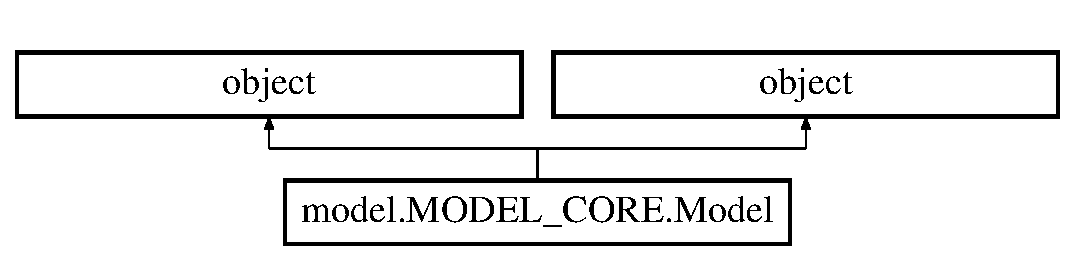
\includegraphics[height=2.000000cm]{classmodel_1_1MODEL__CORE_1_1Model}
\end{center}
\end{figure}
\subsection*{Public Member Functions}
\begin{DoxyCompactItemize}
\item 
def \hyperlink{classmodel_1_1MODEL__CORE_1_1Model_a1176b19897a48d0ad5caa2206abc48c2}{\+\_\+\+\_\+init\+\_\+\+\_\+}
\item 
def \hyperlink{classmodel_1_1MODEL__CORE_1_1Model_a3ef7c7b720e9dc220758de25f1ec8e62}{add\+Parent}
\item 
def \hyperlink{classmodel_1_1MODEL__CORE_1_1Model_a0ce62fa25018f20b53b36b38d73f61c3}{add\+Child}
\item 
def \hyperlink{classmodel_1_1MODEL__CORE_1_1Model_a1176b19897a48d0ad5caa2206abc48c2}{\+\_\+\+\_\+init\+\_\+\+\_\+}
\item 
def \hyperlink{classmodel_1_1MODEL__CORE_1_1Model_a3ef7c7b720e9dc220758de25f1ec8e62}{add\+Parent}
\item 
def \hyperlink{classmodel_1_1MODEL__CORE_1_1Model_a0ce62fa25018f20b53b36b38d73f61c3}{add\+Child}
\end{DoxyCompactItemize}
\subsection*{Public Attributes}
\begin{DoxyCompactItemize}
\item 
\hyperlink{classmodel_1_1MODEL__CORE_1_1Model_adef94b9beef9e75387319ac303823d1e}{name}
\item 
\hyperlink{classmodel_1_1MODEL__CORE_1_1Model_aa25b1292a953fba30ad2bd5bd895fba6}{arg}
\item 
\hyperlink{classmodel_1_1MODEL__CORE_1_1Model_a825d8f80266a50175b837454e720edea}{parents}
\item 
\hyperlink{classmodel_1_1MODEL__CORE_1_1Model_a4d0bad8b1bea374b88baeebe5faf3e5c}{child}
\item 
\hyperlink{classmodel_1_1MODEL__CORE_1_1Model_a3cd14a8cfe0b78fe365e968d2f535bb3}{value}
\end{DoxyCompactItemize}


\subsection{Constructor \& Destructor Documentation}
\hypertarget{classmodel_1_1MODEL__CORE_1_1Model_a1176b19897a48d0ad5caa2206abc48c2}{}\index{model\+::\+M\+O\+D\+E\+L\+\_\+\+C\+O\+R\+E\+::\+Model@{model\+::\+M\+O\+D\+E\+L\+\_\+\+C\+O\+R\+E\+::\+Model}!\+\_\+\+\_\+init\+\_\+\+\_\+@{\+\_\+\+\_\+init\+\_\+\+\_\+}}
\index{\+\_\+\+\_\+init\+\_\+\+\_\+@{\+\_\+\+\_\+init\+\_\+\+\_\+}!model\+::\+M\+O\+D\+E\+L\+\_\+\+C\+O\+R\+E\+::\+Model@{model\+::\+M\+O\+D\+E\+L\+\_\+\+C\+O\+R\+E\+::\+Model}}
\subsubsection[{\+\_\+\+\_\+init\+\_\+\+\_\+}]{\setlength{\rightskip}{0pt plus 5cm}def model.\+M\+O\+D\+E\+L\+\_\+\+C\+O\+R\+E.\+Model.\+\_\+\+\_\+init\+\_\+\+\_\+ (
\begin{DoxyParamCaption}
\item[{}]{self, }
\item[{}]{name, }
\item[{}]{arg = {\ttfamily None}}
\end{DoxyParamCaption}
)}\label{classmodel_1_1MODEL__CORE_1_1Model_a1176b19897a48d0ad5caa2206abc48c2}
\hypertarget{classmodel_1_1MODEL__CORE_1_1Model_a1176b19897a48d0ad5caa2206abc48c2}{}\index{model\+::\+M\+O\+D\+E\+L\+\_\+\+C\+O\+R\+E\+::\+Model@{model\+::\+M\+O\+D\+E\+L\+\_\+\+C\+O\+R\+E\+::\+Model}!\+\_\+\+\_\+init\+\_\+\+\_\+@{\+\_\+\+\_\+init\+\_\+\+\_\+}}
\index{\+\_\+\+\_\+init\+\_\+\+\_\+@{\+\_\+\+\_\+init\+\_\+\+\_\+}!model\+::\+M\+O\+D\+E\+L\+\_\+\+C\+O\+R\+E\+::\+Model@{model\+::\+M\+O\+D\+E\+L\+\_\+\+C\+O\+R\+E\+::\+Model}}
\subsubsection[{\+\_\+\+\_\+init\+\_\+\+\_\+}]{\setlength{\rightskip}{0pt plus 5cm}def model.\+M\+O\+D\+E\+L\+\_\+\+C\+O\+R\+E.\+Model.\+\_\+\+\_\+init\+\_\+\+\_\+ (
\begin{DoxyParamCaption}
\item[{}]{self, }
\item[{}]{name, }
\item[{}]{arg = {\ttfamily None}}
\end{DoxyParamCaption}
)}\label{classmodel_1_1MODEL__CORE_1_1Model_a1176b19897a48d0ad5caa2206abc48c2}


\subsection{Member Function Documentation}
\hypertarget{classmodel_1_1MODEL__CORE_1_1Model_a0ce62fa25018f20b53b36b38d73f61c3}{}\index{model\+::\+M\+O\+D\+E\+L\+\_\+\+C\+O\+R\+E\+::\+Model@{model\+::\+M\+O\+D\+E\+L\+\_\+\+C\+O\+R\+E\+::\+Model}!add\+Child@{add\+Child}}
\index{add\+Child@{add\+Child}!model\+::\+M\+O\+D\+E\+L\+\_\+\+C\+O\+R\+E\+::\+Model@{model\+::\+M\+O\+D\+E\+L\+\_\+\+C\+O\+R\+E\+::\+Model}}
\subsubsection[{add\+Child}]{\setlength{\rightskip}{0pt plus 5cm}def model.\+M\+O\+D\+E\+L\+\_\+\+C\+O\+R\+E.\+Model.\+add\+Child (
\begin{DoxyParamCaption}
\item[{}]{self, }
\item[{}]{child}
\end{DoxyParamCaption}
)}\label{classmodel_1_1MODEL__CORE_1_1Model_a0ce62fa25018f20b53b36b38d73f61c3}
\hypertarget{classmodel_1_1MODEL__CORE_1_1Model_a0ce62fa25018f20b53b36b38d73f61c3}{}\index{model\+::\+M\+O\+D\+E\+L\+\_\+\+C\+O\+R\+E\+::\+Model@{model\+::\+M\+O\+D\+E\+L\+\_\+\+C\+O\+R\+E\+::\+Model}!add\+Child@{add\+Child}}
\index{add\+Child@{add\+Child}!model\+::\+M\+O\+D\+E\+L\+\_\+\+C\+O\+R\+E\+::\+Model@{model\+::\+M\+O\+D\+E\+L\+\_\+\+C\+O\+R\+E\+::\+Model}}
\subsubsection[{add\+Child}]{\setlength{\rightskip}{0pt plus 5cm}def model.\+M\+O\+D\+E\+L\+\_\+\+C\+O\+R\+E.\+Model.\+add\+Child (
\begin{DoxyParamCaption}
\item[{}]{self, }
\item[{}]{child}
\end{DoxyParamCaption}
)}\label{classmodel_1_1MODEL__CORE_1_1Model_a0ce62fa25018f20b53b36b38d73f61c3}
\hypertarget{classmodel_1_1MODEL__CORE_1_1Model_a3ef7c7b720e9dc220758de25f1ec8e62}{}\index{model\+::\+M\+O\+D\+E\+L\+\_\+\+C\+O\+R\+E\+::\+Model@{model\+::\+M\+O\+D\+E\+L\+\_\+\+C\+O\+R\+E\+::\+Model}!add\+Parent@{add\+Parent}}
\index{add\+Parent@{add\+Parent}!model\+::\+M\+O\+D\+E\+L\+\_\+\+C\+O\+R\+E\+::\+Model@{model\+::\+M\+O\+D\+E\+L\+\_\+\+C\+O\+R\+E\+::\+Model}}
\subsubsection[{add\+Parent}]{\setlength{\rightskip}{0pt plus 5cm}def model.\+M\+O\+D\+E\+L\+\_\+\+C\+O\+R\+E.\+Model.\+add\+Parent (
\begin{DoxyParamCaption}
\item[{}]{self, }
\item[{}]{parent}
\end{DoxyParamCaption}
)}\label{classmodel_1_1MODEL__CORE_1_1Model_a3ef7c7b720e9dc220758de25f1ec8e62}
\hypertarget{classmodel_1_1MODEL__CORE_1_1Model_a3ef7c7b720e9dc220758de25f1ec8e62}{}\index{model\+::\+M\+O\+D\+E\+L\+\_\+\+C\+O\+R\+E\+::\+Model@{model\+::\+M\+O\+D\+E\+L\+\_\+\+C\+O\+R\+E\+::\+Model}!add\+Parent@{add\+Parent}}
\index{add\+Parent@{add\+Parent}!model\+::\+M\+O\+D\+E\+L\+\_\+\+C\+O\+R\+E\+::\+Model@{model\+::\+M\+O\+D\+E\+L\+\_\+\+C\+O\+R\+E\+::\+Model}}
\subsubsection[{add\+Parent}]{\setlength{\rightskip}{0pt plus 5cm}def model.\+M\+O\+D\+E\+L\+\_\+\+C\+O\+R\+E.\+Model.\+add\+Parent (
\begin{DoxyParamCaption}
\item[{}]{self, }
\item[{}]{parent}
\end{DoxyParamCaption}
)}\label{classmodel_1_1MODEL__CORE_1_1Model_a3ef7c7b720e9dc220758de25f1ec8e62}


\subsection{Member Data Documentation}
\hypertarget{classmodel_1_1MODEL__CORE_1_1Model_aa25b1292a953fba30ad2bd5bd895fba6}{}\index{model\+::\+M\+O\+D\+E\+L\+\_\+\+C\+O\+R\+E\+::\+Model@{model\+::\+M\+O\+D\+E\+L\+\_\+\+C\+O\+R\+E\+::\+Model}!arg@{arg}}
\index{arg@{arg}!model\+::\+M\+O\+D\+E\+L\+\_\+\+C\+O\+R\+E\+::\+Model@{model\+::\+M\+O\+D\+E\+L\+\_\+\+C\+O\+R\+E\+::\+Model}}
\subsubsection[{arg}]{\setlength{\rightskip}{0pt plus 5cm}model.\+M\+O\+D\+E\+L\+\_\+\+C\+O\+R\+E.\+Model.\+arg}\label{classmodel_1_1MODEL__CORE_1_1Model_aa25b1292a953fba30ad2bd5bd895fba6}
\hypertarget{classmodel_1_1MODEL__CORE_1_1Model_a4d0bad8b1bea374b88baeebe5faf3e5c}{}\index{model\+::\+M\+O\+D\+E\+L\+\_\+\+C\+O\+R\+E\+::\+Model@{model\+::\+M\+O\+D\+E\+L\+\_\+\+C\+O\+R\+E\+::\+Model}!child@{child}}
\index{child@{child}!model\+::\+M\+O\+D\+E\+L\+\_\+\+C\+O\+R\+E\+::\+Model@{model\+::\+M\+O\+D\+E\+L\+\_\+\+C\+O\+R\+E\+::\+Model}}
\subsubsection[{child}]{\setlength{\rightskip}{0pt plus 5cm}model.\+M\+O\+D\+E\+L\+\_\+\+C\+O\+R\+E.\+Model.\+child}\label{classmodel_1_1MODEL__CORE_1_1Model_a4d0bad8b1bea374b88baeebe5faf3e5c}
\hypertarget{classmodel_1_1MODEL__CORE_1_1Model_adef94b9beef9e75387319ac303823d1e}{}\index{model\+::\+M\+O\+D\+E\+L\+\_\+\+C\+O\+R\+E\+::\+Model@{model\+::\+M\+O\+D\+E\+L\+\_\+\+C\+O\+R\+E\+::\+Model}!name@{name}}
\index{name@{name}!model\+::\+M\+O\+D\+E\+L\+\_\+\+C\+O\+R\+E\+::\+Model@{model\+::\+M\+O\+D\+E\+L\+\_\+\+C\+O\+R\+E\+::\+Model}}
\subsubsection[{name}]{\setlength{\rightskip}{0pt plus 5cm}model.\+M\+O\+D\+E\+L\+\_\+\+C\+O\+R\+E.\+Model.\+name}\label{classmodel_1_1MODEL__CORE_1_1Model_adef94b9beef9e75387319ac303823d1e}
\hypertarget{classmodel_1_1MODEL__CORE_1_1Model_a825d8f80266a50175b837454e720edea}{}\index{model\+::\+M\+O\+D\+E\+L\+\_\+\+C\+O\+R\+E\+::\+Model@{model\+::\+M\+O\+D\+E\+L\+\_\+\+C\+O\+R\+E\+::\+Model}!parents@{parents}}
\index{parents@{parents}!model\+::\+M\+O\+D\+E\+L\+\_\+\+C\+O\+R\+E\+::\+Model@{model\+::\+M\+O\+D\+E\+L\+\_\+\+C\+O\+R\+E\+::\+Model}}
\subsubsection[{parents}]{\setlength{\rightskip}{0pt plus 5cm}model.\+M\+O\+D\+E\+L\+\_\+\+C\+O\+R\+E.\+Model.\+parents}\label{classmodel_1_1MODEL__CORE_1_1Model_a825d8f80266a50175b837454e720edea}
\hypertarget{classmodel_1_1MODEL__CORE_1_1Model_a3cd14a8cfe0b78fe365e968d2f535bb3}{}\index{model\+::\+M\+O\+D\+E\+L\+\_\+\+C\+O\+R\+E\+::\+Model@{model\+::\+M\+O\+D\+E\+L\+\_\+\+C\+O\+R\+E\+::\+Model}!value@{value}}
\index{value@{value}!model\+::\+M\+O\+D\+E\+L\+\_\+\+C\+O\+R\+E\+::\+Model@{model\+::\+M\+O\+D\+E\+L\+\_\+\+C\+O\+R\+E\+::\+Model}}
\subsubsection[{value}]{\setlength{\rightskip}{0pt plus 5cm}model.\+M\+O\+D\+E\+L\+\_\+\+C\+O\+R\+E.\+Model.\+value}\label{classmodel_1_1MODEL__CORE_1_1Model_a3cd14a8cfe0b78fe365e968d2f535bb3}


The documentation for this class was generated from the following file\+:\begin{DoxyCompactItemize}
\item 
build/lib.\+linux-\/x86\+\_\+64-\/2.\+7/model/\hyperlink{build_2lib_8linux-x86__64-2_87_2model_2MODEL__CORE_8py}{M\+O\+D\+E\+L\+\_\+\+C\+O\+R\+E.\+py}\end{DoxyCompactItemize}

\hypertarget{classcontroller_1_1MPS__CONTROLLER_1_1MPS}{}\section{controller.\+M\+P\+S\+\_\+\+C\+O\+N\+T\+R\+O\+L\+L\+E\+R.\+M\+P\+S Class Reference}
\label{classcontroller_1_1MPS__CONTROLLER_1_1MPS}\index{controller.\+M\+P\+S\+\_\+\+C\+O\+N\+T\+R\+O\+L\+L\+E\+R.\+M\+P\+S@{controller.\+M\+P\+S\+\_\+\+C\+O\+N\+T\+R\+O\+L\+L\+E\+R.\+M\+P\+S}}
Inheritance diagram for controller.\+M\+P\+S\+\_\+\+C\+O\+N\+T\+R\+O\+L\+L\+E\+R.\+M\+P\+S\+:\begin{figure}[H]
\begin{center}
\leavevmode
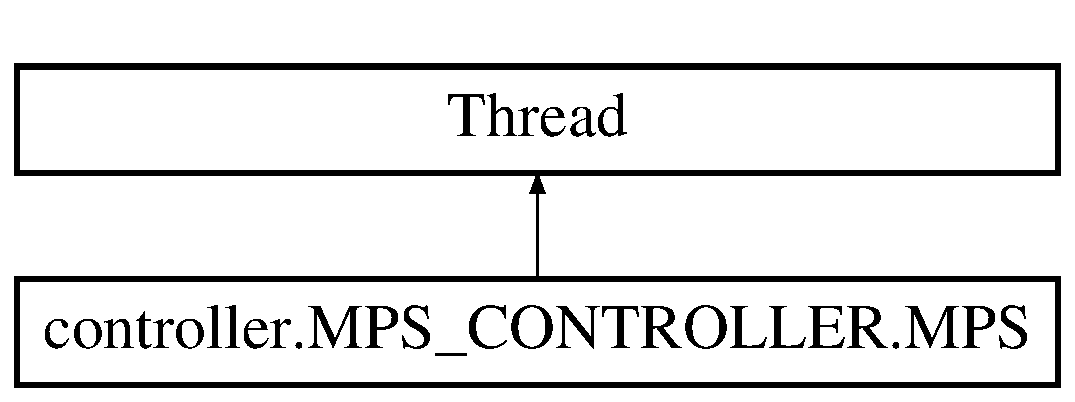
\includegraphics[height=2.000000cm]{classcontroller_1_1MPS__CONTROLLER_1_1MPS}
\end{center}
\end{figure}
\subsection*{Public Member Functions}
\begin{DoxyCompactItemize}
\item 
def \hyperlink{classcontroller_1_1MPS__CONTROLLER_1_1MPS_a1d1173e338a822b9fb79f2729a5b22d6}{\+\_\+\+\_\+init\+\_\+\+\_\+}
\end{DoxyCompactItemize}
\subsection*{Public Attributes}
\begin{DoxyCompactItemize}
\item 
\hyperlink{classcontroller_1_1MPS__CONTROLLER_1_1MPS_a9de44ffe2a85ef6e94382e4cd83edbf4}{num}
\item 
\hyperlink{classcontroller_1_1MPS__CONTROLLER_1_1MPS_a1f68071cc37bb25d2118c03d7c6053de}{parent}
\item 
\hyperlink{classcontroller_1_1MPS__CONTROLLER_1_1MPS_ac4d5522cfd6410de5479c5adaa69445d}{model}
\end{DoxyCompactItemize}


\subsection{Constructor \& Destructor Documentation}
\hypertarget{classcontroller_1_1MPS__CONTROLLER_1_1MPS_a1d1173e338a822b9fb79f2729a5b22d6}{}\index{controller\+::\+M\+P\+S\+\_\+\+C\+O\+N\+T\+R\+O\+L\+L\+E\+R\+::\+M\+P\+S@{controller\+::\+M\+P\+S\+\_\+\+C\+O\+N\+T\+R\+O\+L\+L\+E\+R\+::\+M\+P\+S}!\+\_\+\+\_\+init\+\_\+\+\_\+@{\+\_\+\+\_\+init\+\_\+\+\_\+}}
\index{\+\_\+\+\_\+init\+\_\+\+\_\+@{\+\_\+\+\_\+init\+\_\+\+\_\+}!controller\+::\+M\+P\+S\+\_\+\+C\+O\+N\+T\+R\+O\+L\+L\+E\+R\+::\+M\+P\+S@{controller\+::\+M\+P\+S\+\_\+\+C\+O\+N\+T\+R\+O\+L\+L\+E\+R\+::\+M\+P\+S}}
\subsubsection[{\+\_\+\+\_\+init\+\_\+\+\_\+}]{\setlength{\rightskip}{0pt plus 5cm}def controller.\+M\+P\+S\+\_\+\+C\+O\+N\+T\+R\+O\+L\+L\+E\+R.\+M\+P\+S.\+\_\+\+\_\+init\+\_\+\+\_\+ (
\begin{DoxyParamCaption}
\item[{}]{self, }
\item[{}]{M\+O\+D\+E\+L}
\end{DoxyParamCaption}
)}\label{classcontroller_1_1MPS__CONTROLLER_1_1MPS_a1d1173e338a822b9fb79f2729a5b22d6}


\subsection{Member Data Documentation}
\hypertarget{classcontroller_1_1MPS__CONTROLLER_1_1MPS_ac4d5522cfd6410de5479c5adaa69445d}{}\index{controller\+::\+M\+P\+S\+\_\+\+C\+O\+N\+T\+R\+O\+L\+L\+E\+R\+::\+M\+P\+S@{controller\+::\+M\+P\+S\+\_\+\+C\+O\+N\+T\+R\+O\+L\+L\+E\+R\+::\+M\+P\+S}!model@{model}}
\index{model@{model}!controller\+::\+M\+P\+S\+\_\+\+C\+O\+N\+T\+R\+O\+L\+L\+E\+R\+::\+M\+P\+S@{controller\+::\+M\+P\+S\+\_\+\+C\+O\+N\+T\+R\+O\+L\+L\+E\+R\+::\+M\+P\+S}}
\subsubsection[{model}]{\setlength{\rightskip}{0pt plus 5cm}controller.\+M\+P\+S\+\_\+\+C\+O\+N\+T\+R\+O\+L\+L\+E\+R.\+M\+P\+S.\+model}\label{classcontroller_1_1MPS__CONTROLLER_1_1MPS_ac4d5522cfd6410de5479c5adaa69445d}
\hypertarget{classcontroller_1_1MPS__CONTROLLER_1_1MPS_a9de44ffe2a85ef6e94382e4cd83edbf4}{}\index{controller\+::\+M\+P\+S\+\_\+\+C\+O\+N\+T\+R\+O\+L\+L\+E\+R\+::\+M\+P\+S@{controller\+::\+M\+P\+S\+\_\+\+C\+O\+N\+T\+R\+O\+L\+L\+E\+R\+::\+M\+P\+S}!num@{num}}
\index{num@{num}!controller\+::\+M\+P\+S\+\_\+\+C\+O\+N\+T\+R\+O\+L\+L\+E\+R\+::\+M\+P\+S@{controller\+::\+M\+P\+S\+\_\+\+C\+O\+N\+T\+R\+O\+L\+L\+E\+R\+::\+M\+P\+S}}
\subsubsection[{num}]{\setlength{\rightskip}{0pt plus 5cm}controller.\+M\+P\+S\+\_\+\+C\+O\+N\+T\+R\+O\+L\+L\+E\+R.\+M\+P\+S.\+num}\label{classcontroller_1_1MPS__CONTROLLER_1_1MPS_a9de44ffe2a85ef6e94382e4cd83edbf4}
\hypertarget{classcontroller_1_1MPS__CONTROLLER_1_1MPS_a1f68071cc37bb25d2118c03d7c6053de}{}\index{controller\+::\+M\+P\+S\+\_\+\+C\+O\+N\+T\+R\+O\+L\+L\+E\+R\+::\+M\+P\+S@{controller\+::\+M\+P\+S\+\_\+\+C\+O\+N\+T\+R\+O\+L\+L\+E\+R\+::\+M\+P\+S}!parent@{parent}}
\index{parent@{parent}!controller\+::\+M\+P\+S\+\_\+\+C\+O\+N\+T\+R\+O\+L\+L\+E\+R\+::\+M\+P\+S@{controller\+::\+M\+P\+S\+\_\+\+C\+O\+N\+T\+R\+O\+L\+L\+E\+R\+::\+M\+P\+S}}
\subsubsection[{parent}]{\setlength{\rightskip}{0pt plus 5cm}controller.\+M\+P\+S\+\_\+\+C\+O\+N\+T\+R\+O\+L\+L\+E\+R.\+M\+P\+S.\+parent}\label{classcontroller_1_1MPS__CONTROLLER_1_1MPS_a1f68071cc37bb25d2118c03d7c6053de}


The documentation for this class was generated from the following file\+:\begin{DoxyCompactItemize}
\item 
controller/\hyperlink{MPS__CONTROLLER_8py}{M\+P\+S\+\_\+\+C\+O\+N\+T\+R\+O\+L\+L\+E\+R.\+py}\end{DoxyCompactItemize}

\hypertarget{classinterface_1_1MPS__INTERFACE_1_1MPS}{}\section{interface.\+M\+P\+S\+\_\+\+I\+N\+T\+E\+R\+F\+A\+C\+E.\+M\+P\+S Class Reference}
\label{classinterface_1_1MPS__INTERFACE_1_1MPS}\index{interface.\+M\+P\+S\+\_\+\+I\+N\+T\+E\+R\+F\+A\+C\+E.\+M\+P\+S@{interface.\+M\+P\+S\+\_\+\+I\+N\+T\+E\+R\+F\+A\+C\+E.\+M\+P\+S}}
Inheritance diagram for interface.\+M\+P\+S\+\_\+\+I\+N\+T\+E\+R\+F\+A\+C\+E.\+M\+P\+S\+:\begin{figure}[H]
\begin{center}
\leavevmode
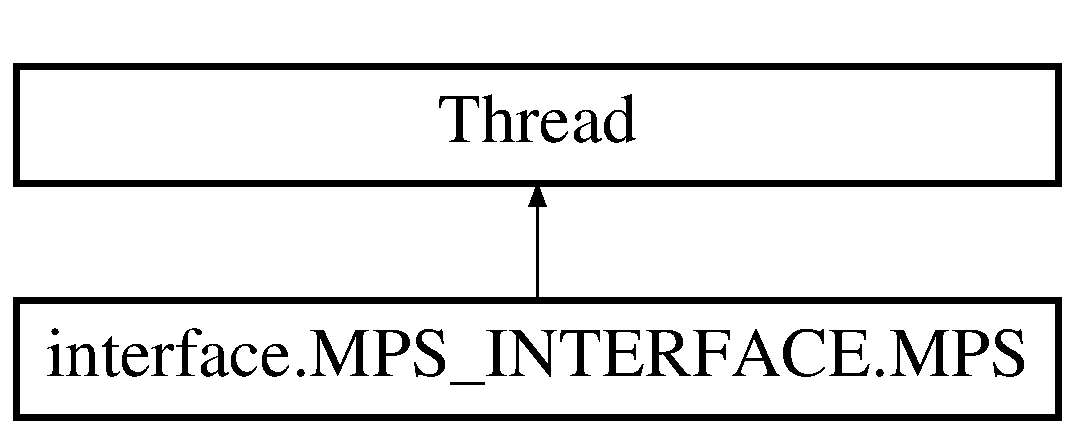
\includegraphics[height=2.000000cm]{classinterface_1_1MPS__INTERFACE_1_1MPS}
\end{center}
\end{figure}
\subsection*{Public Member Functions}
\begin{DoxyCompactItemize}
\item 
def \hyperlink{classinterface_1_1MPS__INTERFACE_1_1MPS_a14e3c3c0348bd54317bf9883cec18bfd}{\+\_\+\+\_\+init\+\_\+\+\_\+}
\item 
def \hyperlink{classinterface_1_1MPS__INTERFACE_1_1MPS_afd3839277bb37e6e365b3bdbce3600b6}{run}
\item 
def \hyperlink{classinterface_1_1MPS__INTERFACE_1_1MPS_ae4d0a8cf4c577cf42c9e1948b5fedee9}{end}
\item 
def \hyperlink{classinterface_1_1MPS__INTERFACE_1_1MPS_af1b0852de8806b27592dab79d44a2916}{hardware\+Display}
\item 
def \hyperlink{classinterface_1_1MPS__INTERFACE_1_1MPS_aab098096679e010e58c2d3b20bd66ca4}{bio\+Display}
\item 
def \hyperlink{classinterface_1_1MPS__INTERFACE_1_1MPS_ad7aa0a5e40c93b9d818730655523db1e}{nav\+Display}
\item 
def \hyperlink{classinterface_1_1MPS__INTERFACE_1_1MPS_a14e3c3c0348bd54317bf9883cec18bfd}{\+\_\+\+\_\+init\+\_\+\+\_\+}
\item 
def \hyperlink{classinterface_1_1MPS__INTERFACE_1_1MPS_afd3839277bb37e6e365b3bdbce3600b6}{run}
\item 
def \hyperlink{classinterface_1_1MPS__INTERFACE_1_1MPS_ae4d0a8cf4c577cf42c9e1948b5fedee9}{end}
\item 
def \hyperlink{classinterface_1_1MPS__INTERFACE_1_1MPS_af1b0852de8806b27592dab79d44a2916}{hardware\+Display}
\item 
def \hyperlink{classinterface_1_1MPS__INTERFACE_1_1MPS_aab098096679e010e58c2d3b20bd66ca4}{bio\+Display}
\item 
def \hyperlink{classinterface_1_1MPS__INTERFACE_1_1MPS_ad7aa0a5e40c93b9d818730655523db1e}{nav\+Display}
\end{DoxyCompactItemize}
\subsection*{Public Attributes}
\begin{DoxyCompactItemize}
\item 
\hyperlink{classinterface_1_1MPS__INTERFACE_1_1MPS_a2a4115fef0beac3a7d779288752ce249}{is\+Running}
\item 
\hyperlink{classinterface_1_1MPS__INTERFACE_1_1MPS_adb8db32687598440ce7e66216e8c748e}{num}
\item 
\hyperlink{classinterface_1_1MPS__INTERFACE_1_1MPS_a291026e13d2fa952fde4a49e17d9b511}{H\+A\+R\+D\+W\+A\+R\+E}
\item 
\hyperlink{classinterface_1_1MPS__INTERFACE_1_1MPS_aeabafb17f8e9cf955bfd72b0b3529a25}{B\+I\+O\+M\+E\+T\+R\+I\+C\+S}
\item 
\hyperlink{classinterface_1_1MPS__INTERFACE_1_1MPS_a3a8859fee065b85d96d5ee4328d4df94}{N\+A\+V}
\item 
\hyperlink{classinterface_1_1MPS__INTERFACE_1_1MPS_ac894fc32b9abb11f2630acbfc8986ec6}{parent}
\item 
\hyperlink{classinterface_1_1MPS__INTERFACE_1_1MPS_a37d1576fdc76e650eba03579715397ec}{display}
\item 
\hyperlink{classinterface_1_1MPS__INTERFACE_1_1MPS_a225f5d63503bd40f580fa9a9dcd3e84c}{link\+Tag}
\item 
\hyperlink{classinterface_1_1MPS__INTERFACE_1_1MPS_a7290342997a971ce72256ac74b88a2cd}{temp\+Tag}
\item 
\hyperlink{classinterface_1_1MPS__INTERFACE_1_1MPS_a8f88b02a8164ee47e8597c3a51b81db6}{lcd}
\item 
\hyperlink{classinterface_1_1MPS__INTERFACE_1_1MPS_ad79d277868987caa37c3026503feb744}{link}
\end{DoxyCompactItemize}


\subsection{Constructor \& Destructor Documentation}
\hypertarget{classinterface_1_1MPS__INTERFACE_1_1MPS_a14e3c3c0348bd54317bf9883cec18bfd}{}\index{interface\+::\+M\+P\+S\+\_\+\+I\+N\+T\+E\+R\+F\+A\+C\+E\+::\+M\+P\+S@{interface\+::\+M\+P\+S\+\_\+\+I\+N\+T\+E\+R\+F\+A\+C\+E\+::\+M\+P\+S}!\+\_\+\+\_\+init\+\_\+\+\_\+@{\+\_\+\+\_\+init\+\_\+\+\_\+}}
\index{\+\_\+\+\_\+init\+\_\+\+\_\+@{\+\_\+\+\_\+init\+\_\+\+\_\+}!interface\+::\+M\+P\+S\+\_\+\+I\+N\+T\+E\+R\+F\+A\+C\+E\+::\+M\+P\+S@{interface\+::\+M\+P\+S\+\_\+\+I\+N\+T\+E\+R\+F\+A\+C\+E\+::\+M\+P\+S}}
\subsubsection[{\+\_\+\+\_\+init\+\_\+\+\_\+}]{\setlength{\rightskip}{0pt plus 5cm}def interface.\+M\+P\+S\+\_\+\+I\+N\+T\+E\+R\+F\+A\+C\+E.\+M\+P\+S.\+\_\+\+\_\+init\+\_\+\+\_\+ (
\begin{DoxyParamCaption}
\item[{}]{self}
\end{DoxyParamCaption}
)}\label{classinterface_1_1MPS__INTERFACE_1_1MPS_a14e3c3c0348bd54317bf9883cec18bfd}
\hypertarget{classinterface_1_1MPS__INTERFACE_1_1MPS_a14e3c3c0348bd54317bf9883cec18bfd}{}\index{interface\+::\+M\+P\+S\+\_\+\+I\+N\+T\+E\+R\+F\+A\+C\+E\+::\+M\+P\+S@{interface\+::\+M\+P\+S\+\_\+\+I\+N\+T\+E\+R\+F\+A\+C\+E\+::\+M\+P\+S}!\+\_\+\+\_\+init\+\_\+\+\_\+@{\+\_\+\+\_\+init\+\_\+\+\_\+}}
\index{\+\_\+\+\_\+init\+\_\+\+\_\+@{\+\_\+\+\_\+init\+\_\+\+\_\+}!interface\+::\+M\+P\+S\+\_\+\+I\+N\+T\+E\+R\+F\+A\+C\+E\+::\+M\+P\+S@{interface\+::\+M\+P\+S\+\_\+\+I\+N\+T\+E\+R\+F\+A\+C\+E\+::\+M\+P\+S}}
\subsubsection[{\+\_\+\+\_\+init\+\_\+\+\_\+}]{\setlength{\rightskip}{0pt plus 5cm}def interface.\+M\+P\+S\+\_\+\+I\+N\+T\+E\+R\+F\+A\+C\+E.\+M\+P\+S.\+\_\+\+\_\+init\+\_\+\+\_\+ (
\begin{DoxyParamCaption}
\item[{}]{self}
\end{DoxyParamCaption}
)}\label{classinterface_1_1MPS__INTERFACE_1_1MPS_a14e3c3c0348bd54317bf9883cec18bfd}


\subsection{Member Function Documentation}
\hypertarget{classinterface_1_1MPS__INTERFACE_1_1MPS_aab098096679e010e58c2d3b20bd66ca4}{}\index{interface\+::\+M\+P\+S\+\_\+\+I\+N\+T\+E\+R\+F\+A\+C\+E\+::\+M\+P\+S@{interface\+::\+M\+P\+S\+\_\+\+I\+N\+T\+E\+R\+F\+A\+C\+E\+::\+M\+P\+S}!bio\+Display@{bio\+Display}}
\index{bio\+Display@{bio\+Display}!interface\+::\+M\+P\+S\+\_\+\+I\+N\+T\+E\+R\+F\+A\+C\+E\+::\+M\+P\+S@{interface\+::\+M\+P\+S\+\_\+\+I\+N\+T\+E\+R\+F\+A\+C\+E\+::\+M\+P\+S}}
\subsubsection[{bio\+Display}]{\setlength{\rightskip}{0pt plus 5cm}def interface.\+M\+P\+S\+\_\+\+I\+N\+T\+E\+R\+F\+A\+C\+E.\+M\+P\+S.\+bio\+Display (
\begin{DoxyParamCaption}
\item[{}]{self}
\end{DoxyParamCaption}
)}\label{classinterface_1_1MPS__INTERFACE_1_1MPS_aab098096679e010e58c2d3b20bd66ca4}
\hypertarget{classinterface_1_1MPS__INTERFACE_1_1MPS_aab098096679e010e58c2d3b20bd66ca4}{}\index{interface\+::\+M\+P\+S\+\_\+\+I\+N\+T\+E\+R\+F\+A\+C\+E\+::\+M\+P\+S@{interface\+::\+M\+P\+S\+\_\+\+I\+N\+T\+E\+R\+F\+A\+C\+E\+::\+M\+P\+S}!bio\+Display@{bio\+Display}}
\index{bio\+Display@{bio\+Display}!interface\+::\+M\+P\+S\+\_\+\+I\+N\+T\+E\+R\+F\+A\+C\+E\+::\+M\+P\+S@{interface\+::\+M\+P\+S\+\_\+\+I\+N\+T\+E\+R\+F\+A\+C\+E\+::\+M\+P\+S}}
\subsubsection[{bio\+Display}]{\setlength{\rightskip}{0pt plus 5cm}def interface.\+M\+P\+S\+\_\+\+I\+N\+T\+E\+R\+F\+A\+C\+E.\+M\+P\+S.\+bio\+Display (
\begin{DoxyParamCaption}
\item[{}]{self}
\end{DoxyParamCaption}
)}\label{classinterface_1_1MPS__INTERFACE_1_1MPS_aab098096679e010e58c2d3b20bd66ca4}
\hypertarget{classinterface_1_1MPS__INTERFACE_1_1MPS_ae4d0a8cf4c577cf42c9e1948b5fedee9}{}\index{interface\+::\+M\+P\+S\+\_\+\+I\+N\+T\+E\+R\+F\+A\+C\+E\+::\+M\+P\+S@{interface\+::\+M\+P\+S\+\_\+\+I\+N\+T\+E\+R\+F\+A\+C\+E\+::\+M\+P\+S}!end@{end}}
\index{end@{end}!interface\+::\+M\+P\+S\+\_\+\+I\+N\+T\+E\+R\+F\+A\+C\+E\+::\+M\+P\+S@{interface\+::\+M\+P\+S\+\_\+\+I\+N\+T\+E\+R\+F\+A\+C\+E\+::\+M\+P\+S}}
\subsubsection[{end}]{\setlength{\rightskip}{0pt plus 5cm}def interface.\+M\+P\+S\+\_\+\+I\+N\+T\+E\+R\+F\+A\+C\+E.\+M\+P\+S.\+end (
\begin{DoxyParamCaption}
\item[{}]{self}
\end{DoxyParamCaption}
)}\label{classinterface_1_1MPS__INTERFACE_1_1MPS_ae4d0a8cf4c577cf42c9e1948b5fedee9}
\hypertarget{classinterface_1_1MPS__INTERFACE_1_1MPS_ae4d0a8cf4c577cf42c9e1948b5fedee9}{}\index{interface\+::\+M\+P\+S\+\_\+\+I\+N\+T\+E\+R\+F\+A\+C\+E\+::\+M\+P\+S@{interface\+::\+M\+P\+S\+\_\+\+I\+N\+T\+E\+R\+F\+A\+C\+E\+::\+M\+P\+S}!end@{end}}
\index{end@{end}!interface\+::\+M\+P\+S\+\_\+\+I\+N\+T\+E\+R\+F\+A\+C\+E\+::\+M\+P\+S@{interface\+::\+M\+P\+S\+\_\+\+I\+N\+T\+E\+R\+F\+A\+C\+E\+::\+M\+P\+S}}
\subsubsection[{end}]{\setlength{\rightskip}{0pt plus 5cm}def interface.\+M\+P\+S\+\_\+\+I\+N\+T\+E\+R\+F\+A\+C\+E.\+M\+P\+S.\+end (
\begin{DoxyParamCaption}
\item[{}]{self}
\end{DoxyParamCaption}
)}\label{classinterface_1_1MPS__INTERFACE_1_1MPS_ae4d0a8cf4c577cf42c9e1948b5fedee9}
\hypertarget{classinterface_1_1MPS__INTERFACE_1_1MPS_af1b0852de8806b27592dab79d44a2916}{}\index{interface\+::\+M\+P\+S\+\_\+\+I\+N\+T\+E\+R\+F\+A\+C\+E\+::\+M\+P\+S@{interface\+::\+M\+P\+S\+\_\+\+I\+N\+T\+E\+R\+F\+A\+C\+E\+::\+M\+P\+S}!hardware\+Display@{hardware\+Display}}
\index{hardware\+Display@{hardware\+Display}!interface\+::\+M\+P\+S\+\_\+\+I\+N\+T\+E\+R\+F\+A\+C\+E\+::\+M\+P\+S@{interface\+::\+M\+P\+S\+\_\+\+I\+N\+T\+E\+R\+F\+A\+C\+E\+::\+M\+P\+S}}
\subsubsection[{hardware\+Display}]{\setlength{\rightskip}{0pt plus 5cm}def interface.\+M\+P\+S\+\_\+\+I\+N\+T\+E\+R\+F\+A\+C\+E.\+M\+P\+S.\+hardware\+Display (
\begin{DoxyParamCaption}
\item[{}]{self}
\end{DoxyParamCaption}
)}\label{classinterface_1_1MPS__INTERFACE_1_1MPS_af1b0852de8806b27592dab79d44a2916}
\hypertarget{classinterface_1_1MPS__INTERFACE_1_1MPS_af1b0852de8806b27592dab79d44a2916}{}\index{interface\+::\+M\+P\+S\+\_\+\+I\+N\+T\+E\+R\+F\+A\+C\+E\+::\+M\+P\+S@{interface\+::\+M\+P\+S\+\_\+\+I\+N\+T\+E\+R\+F\+A\+C\+E\+::\+M\+P\+S}!hardware\+Display@{hardware\+Display}}
\index{hardware\+Display@{hardware\+Display}!interface\+::\+M\+P\+S\+\_\+\+I\+N\+T\+E\+R\+F\+A\+C\+E\+::\+M\+P\+S@{interface\+::\+M\+P\+S\+\_\+\+I\+N\+T\+E\+R\+F\+A\+C\+E\+::\+M\+P\+S}}
\subsubsection[{hardware\+Display}]{\setlength{\rightskip}{0pt plus 5cm}def interface.\+M\+P\+S\+\_\+\+I\+N\+T\+E\+R\+F\+A\+C\+E.\+M\+P\+S.\+hardware\+Display (
\begin{DoxyParamCaption}
\item[{}]{self}
\end{DoxyParamCaption}
)}\label{classinterface_1_1MPS__INTERFACE_1_1MPS_af1b0852de8806b27592dab79d44a2916}
\hypertarget{classinterface_1_1MPS__INTERFACE_1_1MPS_ad7aa0a5e40c93b9d818730655523db1e}{}\index{interface\+::\+M\+P\+S\+\_\+\+I\+N\+T\+E\+R\+F\+A\+C\+E\+::\+M\+P\+S@{interface\+::\+M\+P\+S\+\_\+\+I\+N\+T\+E\+R\+F\+A\+C\+E\+::\+M\+P\+S}!nav\+Display@{nav\+Display}}
\index{nav\+Display@{nav\+Display}!interface\+::\+M\+P\+S\+\_\+\+I\+N\+T\+E\+R\+F\+A\+C\+E\+::\+M\+P\+S@{interface\+::\+M\+P\+S\+\_\+\+I\+N\+T\+E\+R\+F\+A\+C\+E\+::\+M\+P\+S}}
\subsubsection[{nav\+Display}]{\setlength{\rightskip}{0pt plus 5cm}def interface.\+M\+P\+S\+\_\+\+I\+N\+T\+E\+R\+F\+A\+C\+E.\+M\+P\+S.\+nav\+Display (
\begin{DoxyParamCaption}
\item[{}]{self}
\end{DoxyParamCaption}
)}\label{classinterface_1_1MPS__INTERFACE_1_1MPS_ad7aa0a5e40c93b9d818730655523db1e}
\hypertarget{classinterface_1_1MPS__INTERFACE_1_1MPS_ad7aa0a5e40c93b9d818730655523db1e}{}\index{interface\+::\+M\+P\+S\+\_\+\+I\+N\+T\+E\+R\+F\+A\+C\+E\+::\+M\+P\+S@{interface\+::\+M\+P\+S\+\_\+\+I\+N\+T\+E\+R\+F\+A\+C\+E\+::\+M\+P\+S}!nav\+Display@{nav\+Display}}
\index{nav\+Display@{nav\+Display}!interface\+::\+M\+P\+S\+\_\+\+I\+N\+T\+E\+R\+F\+A\+C\+E\+::\+M\+P\+S@{interface\+::\+M\+P\+S\+\_\+\+I\+N\+T\+E\+R\+F\+A\+C\+E\+::\+M\+P\+S}}
\subsubsection[{nav\+Display}]{\setlength{\rightskip}{0pt plus 5cm}def interface.\+M\+P\+S\+\_\+\+I\+N\+T\+E\+R\+F\+A\+C\+E.\+M\+P\+S.\+nav\+Display (
\begin{DoxyParamCaption}
\item[{}]{self}
\end{DoxyParamCaption}
)}\label{classinterface_1_1MPS__INTERFACE_1_1MPS_ad7aa0a5e40c93b9d818730655523db1e}
\hypertarget{classinterface_1_1MPS__INTERFACE_1_1MPS_afd3839277bb37e6e365b3bdbce3600b6}{}\index{interface\+::\+M\+P\+S\+\_\+\+I\+N\+T\+E\+R\+F\+A\+C\+E\+::\+M\+P\+S@{interface\+::\+M\+P\+S\+\_\+\+I\+N\+T\+E\+R\+F\+A\+C\+E\+::\+M\+P\+S}!run@{run}}
\index{run@{run}!interface\+::\+M\+P\+S\+\_\+\+I\+N\+T\+E\+R\+F\+A\+C\+E\+::\+M\+P\+S@{interface\+::\+M\+P\+S\+\_\+\+I\+N\+T\+E\+R\+F\+A\+C\+E\+::\+M\+P\+S}}
\subsubsection[{run}]{\setlength{\rightskip}{0pt plus 5cm}def interface.\+M\+P\+S\+\_\+\+I\+N\+T\+E\+R\+F\+A\+C\+E.\+M\+P\+S.\+run (
\begin{DoxyParamCaption}
\item[{}]{self}
\end{DoxyParamCaption}
)}\label{classinterface_1_1MPS__INTERFACE_1_1MPS_afd3839277bb37e6e365b3bdbce3600b6}
\hypertarget{classinterface_1_1MPS__INTERFACE_1_1MPS_afd3839277bb37e6e365b3bdbce3600b6}{}\index{interface\+::\+M\+P\+S\+\_\+\+I\+N\+T\+E\+R\+F\+A\+C\+E\+::\+M\+P\+S@{interface\+::\+M\+P\+S\+\_\+\+I\+N\+T\+E\+R\+F\+A\+C\+E\+::\+M\+P\+S}!run@{run}}
\index{run@{run}!interface\+::\+M\+P\+S\+\_\+\+I\+N\+T\+E\+R\+F\+A\+C\+E\+::\+M\+P\+S@{interface\+::\+M\+P\+S\+\_\+\+I\+N\+T\+E\+R\+F\+A\+C\+E\+::\+M\+P\+S}}
\subsubsection[{run}]{\setlength{\rightskip}{0pt plus 5cm}def interface.\+M\+P\+S\+\_\+\+I\+N\+T\+E\+R\+F\+A\+C\+E.\+M\+P\+S.\+run (
\begin{DoxyParamCaption}
\item[{}]{self}
\end{DoxyParamCaption}
)}\label{classinterface_1_1MPS__INTERFACE_1_1MPS_afd3839277bb37e6e365b3bdbce3600b6}


\subsection{Member Data Documentation}
\hypertarget{classinterface_1_1MPS__INTERFACE_1_1MPS_aeabafb17f8e9cf955bfd72b0b3529a25}{}\index{interface\+::\+M\+P\+S\+\_\+\+I\+N\+T\+E\+R\+F\+A\+C\+E\+::\+M\+P\+S@{interface\+::\+M\+P\+S\+\_\+\+I\+N\+T\+E\+R\+F\+A\+C\+E\+::\+M\+P\+S}!B\+I\+O\+M\+E\+T\+R\+I\+C\+S@{B\+I\+O\+M\+E\+T\+R\+I\+C\+S}}
\index{B\+I\+O\+M\+E\+T\+R\+I\+C\+S@{B\+I\+O\+M\+E\+T\+R\+I\+C\+S}!interface\+::\+M\+P\+S\+\_\+\+I\+N\+T\+E\+R\+F\+A\+C\+E\+::\+M\+P\+S@{interface\+::\+M\+P\+S\+\_\+\+I\+N\+T\+E\+R\+F\+A\+C\+E\+::\+M\+P\+S}}
\subsubsection[{B\+I\+O\+M\+E\+T\+R\+I\+C\+S}]{\setlength{\rightskip}{0pt plus 5cm}interface.\+M\+P\+S\+\_\+\+I\+N\+T\+E\+R\+F\+A\+C\+E.\+M\+P\+S.\+B\+I\+O\+M\+E\+T\+R\+I\+C\+S}\label{classinterface_1_1MPS__INTERFACE_1_1MPS_aeabafb17f8e9cf955bfd72b0b3529a25}
\hypertarget{classinterface_1_1MPS__INTERFACE_1_1MPS_a37d1576fdc76e650eba03579715397ec}{}\index{interface\+::\+M\+P\+S\+\_\+\+I\+N\+T\+E\+R\+F\+A\+C\+E\+::\+M\+P\+S@{interface\+::\+M\+P\+S\+\_\+\+I\+N\+T\+E\+R\+F\+A\+C\+E\+::\+M\+P\+S}!display@{display}}
\index{display@{display}!interface\+::\+M\+P\+S\+\_\+\+I\+N\+T\+E\+R\+F\+A\+C\+E\+::\+M\+P\+S@{interface\+::\+M\+P\+S\+\_\+\+I\+N\+T\+E\+R\+F\+A\+C\+E\+::\+M\+P\+S}}
\subsubsection[{display}]{\setlength{\rightskip}{0pt plus 5cm}interface.\+M\+P\+S\+\_\+\+I\+N\+T\+E\+R\+F\+A\+C\+E.\+M\+P\+S.\+display}\label{classinterface_1_1MPS__INTERFACE_1_1MPS_a37d1576fdc76e650eba03579715397ec}
\hypertarget{classinterface_1_1MPS__INTERFACE_1_1MPS_a291026e13d2fa952fde4a49e17d9b511}{}\index{interface\+::\+M\+P\+S\+\_\+\+I\+N\+T\+E\+R\+F\+A\+C\+E\+::\+M\+P\+S@{interface\+::\+M\+P\+S\+\_\+\+I\+N\+T\+E\+R\+F\+A\+C\+E\+::\+M\+P\+S}!H\+A\+R\+D\+W\+A\+R\+E@{H\+A\+R\+D\+W\+A\+R\+E}}
\index{H\+A\+R\+D\+W\+A\+R\+E@{H\+A\+R\+D\+W\+A\+R\+E}!interface\+::\+M\+P\+S\+\_\+\+I\+N\+T\+E\+R\+F\+A\+C\+E\+::\+M\+P\+S@{interface\+::\+M\+P\+S\+\_\+\+I\+N\+T\+E\+R\+F\+A\+C\+E\+::\+M\+P\+S}}
\subsubsection[{H\+A\+R\+D\+W\+A\+R\+E}]{\setlength{\rightskip}{0pt plus 5cm}interface.\+M\+P\+S\+\_\+\+I\+N\+T\+E\+R\+F\+A\+C\+E.\+M\+P\+S.\+H\+A\+R\+D\+W\+A\+R\+E}\label{classinterface_1_1MPS__INTERFACE_1_1MPS_a291026e13d2fa952fde4a49e17d9b511}
\hypertarget{classinterface_1_1MPS__INTERFACE_1_1MPS_a2a4115fef0beac3a7d779288752ce249}{}\index{interface\+::\+M\+P\+S\+\_\+\+I\+N\+T\+E\+R\+F\+A\+C\+E\+::\+M\+P\+S@{interface\+::\+M\+P\+S\+\_\+\+I\+N\+T\+E\+R\+F\+A\+C\+E\+::\+M\+P\+S}!is\+Running@{is\+Running}}
\index{is\+Running@{is\+Running}!interface\+::\+M\+P\+S\+\_\+\+I\+N\+T\+E\+R\+F\+A\+C\+E\+::\+M\+P\+S@{interface\+::\+M\+P\+S\+\_\+\+I\+N\+T\+E\+R\+F\+A\+C\+E\+::\+M\+P\+S}}
\subsubsection[{is\+Running}]{\setlength{\rightskip}{0pt plus 5cm}interface.\+M\+P\+S\+\_\+\+I\+N\+T\+E\+R\+F\+A\+C\+E.\+M\+P\+S.\+is\+Running}\label{classinterface_1_1MPS__INTERFACE_1_1MPS_a2a4115fef0beac3a7d779288752ce249}
\hypertarget{classinterface_1_1MPS__INTERFACE_1_1MPS_a8f88b02a8164ee47e8597c3a51b81db6}{}\index{interface\+::\+M\+P\+S\+\_\+\+I\+N\+T\+E\+R\+F\+A\+C\+E\+::\+M\+P\+S@{interface\+::\+M\+P\+S\+\_\+\+I\+N\+T\+E\+R\+F\+A\+C\+E\+::\+M\+P\+S}!lcd@{lcd}}
\index{lcd@{lcd}!interface\+::\+M\+P\+S\+\_\+\+I\+N\+T\+E\+R\+F\+A\+C\+E\+::\+M\+P\+S@{interface\+::\+M\+P\+S\+\_\+\+I\+N\+T\+E\+R\+F\+A\+C\+E\+::\+M\+P\+S}}
\subsubsection[{lcd}]{\setlength{\rightskip}{0pt plus 5cm}interface.\+M\+P\+S\+\_\+\+I\+N\+T\+E\+R\+F\+A\+C\+E.\+M\+P\+S.\+lcd}\label{classinterface_1_1MPS__INTERFACE_1_1MPS_a8f88b02a8164ee47e8597c3a51b81db6}
\hypertarget{classinterface_1_1MPS__INTERFACE_1_1MPS_ad79d277868987caa37c3026503feb744}{}\index{interface\+::\+M\+P\+S\+\_\+\+I\+N\+T\+E\+R\+F\+A\+C\+E\+::\+M\+P\+S@{interface\+::\+M\+P\+S\+\_\+\+I\+N\+T\+E\+R\+F\+A\+C\+E\+::\+M\+P\+S}!link@{link}}
\index{link@{link}!interface\+::\+M\+P\+S\+\_\+\+I\+N\+T\+E\+R\+F\+A\+C\+E\+::\+M\+P\+S@{interface\+::\+M\+P\+S\+\_\+\+I\+N\+T\+E\+R\+F\+A\+C\+E\+::\+M\+P\+S}}
\subsubsection[{link}]{\setlength{\rightskip}{0pt plus 5cm}interface.\+M\+P\+S\+\_\+\+I\+N\+T\+E\+R\+F\+A\+C\+E.\+M\+P\+S.\+link}\label{classinterface_1_1MPS__INTERFACE_1_1MPS_ad79d277868987caa37c3026503feb744}
\hypertarget{classinterface_1_1MPS__INTERFACE_1_1MPS_a225f5d63503bd40f580fa9a9dcd3e84c}{}\index{interface\+::\+M\+P\+S\+\_\+\+I\+N\+T\+E\+R\+F\+A\+C\+E\+::\+M\+P\+S@{interface\+::\+M\+P\+S\+\_\+\+I\+N\+T\+E\+R\+F\+A\+C\+E\+::\+M\+P\+S}!link\+Tag@{link\+Tag}}
\index{link\+Tag@{link\+Tag}!interface\+::\+M\+P\+S\+\_\+\+I\+N\+T\+E\+R\+F\+A\+C\+E\+::\+M\+P\+S@{interface\+::\+M\+P\+S\+\_\+\+I\+N\+T\+E\+R\+F\+A\+C\+E\+::\+M\+P\+S}}
\subsubsection[{link\+Tag}]{\setlength{\rightskip}{0pt plus 5cm}interface.\+M\+P\+S\+\_\+\+I\+N\+T\+E\+R\+F\+A\+C\+E.\+M\+P\+S.\+link\+Tag}\label{classinterface_1_1MPS__INTERFACE_1_1MPS_a225f5d63503bd40f580fa9a9dcd3e84c}
\hypertarget{classinterface_1_1MPS__INTERFACE_1_1MPS_a3a8859fee065b85d96d5ee4328d4df94}{}\index{interface\+::\+M\+P\+S\+\_\+\+I\+N\+T\+E\+R\+F\+A\+C\+E\+::\+M\+P\+S@{interface\+::\+M\+P\+S\+\_\+\+I\+N\+T\+E\+R\+F\+A\+C\+E\+::\+M\+P\+S}!N\+A\+V@{N\+A\+V}}
\index{N\+A\+V@{N\+A\+V}!interface\+::\+M\+P\+S\+\_\+\+I\+N\+T\+E\+R\+F\+A\+C\+E\+::\+M\+P\+S@{interface\+::\+M\+P\+S\+\_\+\+I\+N\+T\+E\+R\+F\+A\+C\+E\+::\+M\+P\+S}}
\subsubsection[{N\+A\+V}]{\setlength{\rightskip}{0pt plus 5cm}interface.\+M\+P\+S\+\_\+\+I\+N\+T\+E\+R\+F\+A\+C\+E.\+M\+P\+S.\+N\+A\+V}\label{classinterface_1_1MPS__INTERFACE_1_1MPS_a3a8859fee065b85d96d5ee4328d4df94}
\hypertarget{classinterface_1_1MPS__INTERFACE_1_1MPS_adb8db32687598440ce7e66216e8c748e}{}\index{interface\+::\+M\+P\+S\+\_\+\+I\+N\+T\+E\+R\+F\+A\+C\+E\+::\+M\+P\+S@{interface\+::\+M\+P\+S\+\_\+\+I\+N\+T\+E\+R\+F\+A\+C\+E\+::\+M\+P\+S}!num@{num}}
\index{num@{num}!interface\+::\+M\+P\+S\+\_\+\+I\+N\+T\+E\+R\+F\+A\+C\+E\+::\+M\+P\+S@{interface\+::\+M\+P\+S\+\_\+\+I\+N\+T\+E\+R\+F\+A\+C\+E\+::\+M\+P\+S}}
\subsubsection[{num}]{\setlength{\rightskip}{0pt plus 5cm}interface.\+M\+P\+S\+\_\+\+I\+N\+T\+E\+R\+F\+A\+C\+E.\+M\+P\+S.\+num}\label{classinterface_1_1MPS__INTERFACE_1_1MPS_adb8db32687598440ce7e66216e8c748e}
\hypertarget{classinterface_1_1MPS__INTERFACE_1_1MPS_ac894fc32b9abb11f2630acbfc8986ec6}{}\index{interface\+::\+M\+P\+S\+\_\+\+I\+N\+T\+E\+R\+F\+A\+C\+E\+::\+M\+P\+S@{interface\+::\+M\+P\+S\+\_\+\+I\+N\+T\+E\+R\+F\+A\+C\+E\+::\+M\+P\+S}!parent@{parent}}
\index{parent@{parent}!interface\+::\+M\+P\+S\+\_\+\+I\+N\+T\+E\+R\+F\+A\+C\+E\+::\+M\+P\+S@{interface\+::\+M\+P\+S\+\_\+\+I\+N\+T\+E\+R\+F\+A\+C\+E\+::\+M\+P\+S}}
\subsubsection[{parent}]{\setlength{\rightskip}{0pt plus 5cm}interface.\+M\+P\+S\+\_\+\+I\+N\+T\+E\+R\+F\+A\+C\+E.\+M\+P\+S.\+parent}\label{classinterface_1_1MPS__INTERFACE_1_1MPS_ac894fc32b9abb11f2630acbfc8986ec6}
\hypertarget{classinterface_1_1MPS__INTERFACE_1_1MPS_a7290342997a971ce72256ac74b88a2cd}{}\index{interface\+::\+M\+P\+S\+\_\+\+I\+N\+T\+E\+R\+F\+A\+C\+E\+::\+M\+P\+S@{interface\+::\+M\+P\+S\+\_\+\+I\+N\+T\+E\+R\+F\+A\+C\+E\+::\+M\+P\+S}!temp\+Tag@{temp\+Tag}}
\index{temp\+Tag@{temp\+Tag}!interface\+::\+M\+P\+S\+\_\+\+I\+N\+T\+E\+R\+F\+A\+C\+E\+::\+M\+P\+S@{interface\+::\+M\+P\+S\+\_\+\+I\+N\+T\+E\+R\+F\+A\+C\+E\+::\+M\+P\+S}}
\subsubsection[{temp\+Tag}]{\setlength{\rightskip}{0pt plus 5cm}interface.\+M\+P\+S\+\_\+\+I\+N\+T\+E\+R\+F\+A\+C\+E.\+M\+P\+S.\+temp\+Tag}\label{classinterface_1_1MPS__INTERFACE_1_1MPS_a7290342997a971ce72256ac74b88a2cd}


The documentation for this class was generated from the following file\+:\begin{DoxyCompactItemize}
\item 
G\+I\+T-\/\+C\+O\+P\+Y/\+Software/interface/\hyperlink{GIT-COPY_2Software_2interface_2MPS__INTERFACE_8py}{M\+P\+S\+\_\+\+I\+N\+T\+E\+R\+F\+A\+C\+E.\+py}\end{DoxyCompactItemize}

\hypertarget{classinterface_1_1lcd_1_1MPS}{}\section{interface.\+lcd.\+M\+P\+S Class Reference}
\label{classinterface_1_1lcd_1_1MPS}\index{interface.\+lcd.\+M\+P\+S@{interface.\+lcd.\+M\+P\+S}}
Inheritance diagram for interface.\+lcd.\+M\+P\+S\+:\begin{figure}[H]
\begin{center}
\leavevmode
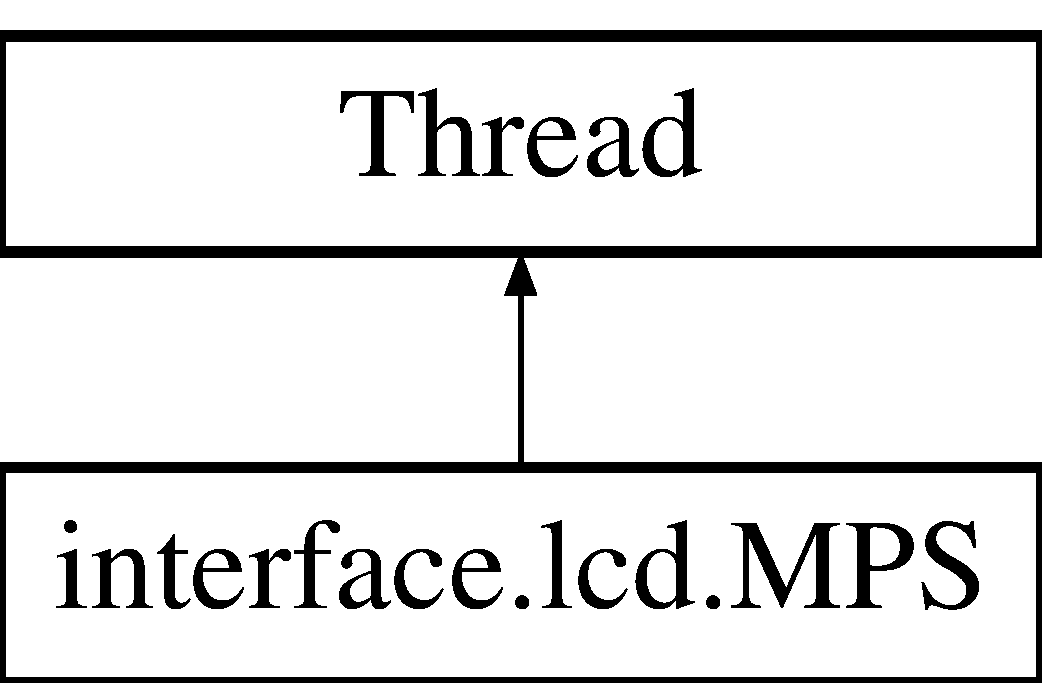
\includegraphics[height=2.000000cm]{classinterface_1_1lcd_1_1MPS}
\end{center}
\end{figure}
\subsection*{Public Member Functions}
\begin{DoxyCompactItemize}
\item 
def \hyperlink{classinterface_1_1lcd_1_1MPS_a52eee073eb72cffe7865fcc59c83bf95}{\+\_\+\+\_\+init\+\_\+\+\_\+}
\item 
def \hyperlink{classinterface_1_1lcd_1_1MPS_a7c696e6242aa5e524a426ce73a8a8050}{run}
\item 
def \hyperlink{classinterface_1_1lcd_1_1MPS_ad9481e02c1fc887aa940144141074bc3}{end}
\item 
def \hyperlink{classinterface_1_1lcd_1_1MPS_a56a76849d7a11e2d4768e8813a6e6c19}{hardware\+Display}
\item 
def \hyperlink{classinterface_1_1lcd_1_1MPS_aa5ae91eb14143474a31fac7754c41228}{bio\+Display}
\item 
def \hyperlink{classinterface_1_1lcd_1_1MPS_a8ea7992a675b520b586cb53d276c6f54}{nav\+Display}
\item 
def \hyperlink{classinterface_1_1lcd_1_1MPS_a52eee073eb72cffe7865fcc59c83bf95}{\+\_\+\+\_\+init\+\_\+\+\_\+}
\item 
def \hyperlink{classinterface_1_1lcd_1_1MPS_a7c696e6242aa5e524a426ce73a8a8050}{run}
\item 
def \hyperlink{classinterface_1_1lcd_1_1MPS_ad9481e02c1fc887aa940144141074bc3}{end}
\item 
def \hyperlink{classinterface_1_1lcd_1_1MPS_a56a76849d7a11e2d4768e8813a6e6c19}{hardware\+Display}
\item 
def \hyperlink{classinterface_1_1lcd_1_1MPS_aa5ae91eb14143474a31fac7754c41228}{bio\+Display}
\item 
def \hyperlink{classinterface_1_1lcd_1_1MPS_a8ea7992a675b520b586cb53d276c6f54}{nav\+Display}
\end{DoxyCompactItemize}
\subsection*{Public Attributes}
\begin{DoxyCompactItemize}
\item 
\hyperlink{classinterface_1_1lcd_1_1MPS_ac189498130bd20b2aa2f6d5ec9c48210}{is\+Running}
\item 
\hyperlink{classinterface_1_1lcd_1_1MPS_a698ac3f1e12c9d6c893c135d06252f66}{num}
\item 
\hyperlink{classinterface_1_1lcd_1_1MPS_a13d4d61510dd6c8a3c40e8517f4156f9}{H\+A\+R\+D\+W\+A\+R\+E}
\item 
\hyperlink{classinterface_1_1lcd_1_1MPS_a8cbbd0d1f225eea64e9a57fba3242413}{B\+I\+O\+M\+E\+T\+R\+I\+C\+S}
\item 
\hyperlink{classinterface_1_1lcd_1_1MPS_a128ad75cc77e06e9621cb8a8d2e4a6e7}{N\+A\+V}
\item 
\hyperlink{classinterface_1_1lcd_1_1MPS_a1d739a8338d7a795b4efa322d08f2808}{parent}
\item 
\hyperlink{classinterface_1_1lcd_1_1MPS_a7c35d293b68239621532f76b0933f6c5}{display}
\item 
\hyperlink{classinterface_1_1lcd_1_1MPS_ac3601f1dd283764baca481f596f6ca40}{lcd}
\end{DoxyCompactItemize}


\subsection{Constructor \& Destructor Documentation}
\hypertarget{classinterface_1_1lcd_1_1MPS_a52eee073eb72cffe7865fcc59c83bf95}{}\index{interface\+::lcd\+::\+M\+P\+S@{interface\+::lcd\+::\+M\+P\+S}!\+\_\+\+\_\+init\+\_\+\+\_\+@{\+\_\+\+\_\+init\+\_\+\+\_\+}}
\index{\+\_\+\+\_\+init\+\_\+\+\_\+@{\+\_\+\+\_\+init\+\_\+\+\_\+}!interface\+::lcd\+::\+M\+P\+S@{interface\+::lcd\+::\+M\+P\+S}}
\subsubsection[{\+\_\+\+\_\+init\+\_\+\+\_\+}]{\setlength{\rightskip}{0pt plus 5cm}def interface.\+lcd.\+M\+P\+S.\+\_\+\+\_\+init\+\_\+\+\_\+ (
\begin{DoxyParamCaption}
\item[{}]{self}
\end{DoxyParamCaption}
)}\label{classinterface_1_1lcd_1_1MPS_a52eee073eb72cffe7865fcc59c83bf95}
\hypertarget{classinterface_1_1lcd_1_1MPS_a52eee073eb72cffe7865fcc59c83bf95}{}\index{interface\+::lcd\+::\+M\+P\+S@{interface\+::lcd\+::\+M\+P\+S}!\+\_\+\+\_\+init\+\_\+\+\_\+@{\+\_\+\+\_\+init\+\_\+\+\_\+}}
\index{\+\_\+\+\_\+init\+\_\+\+\_\+@{\+\_\+\+\_\+init\+\_\+\+\_\+}!interface\+::lcd\+::\+M\+P\+S@{interface\+::lcd\+::\+M\+P\+S}}
\subsubsection[{\+\_\+\+\_\+init\+\_\+\+\_\+}]{\setlength{\rightskip}{0pt plus 5cm}def interface.\+lcd.\+M\+P\+S.\+\_\+\+\_\+init\+\_\+\+\_\+ (
\begin{DoxyParamCaption}
\item[{}]{self}
\end{DoxyParamCaption}
)}\label{classinterface_1_1lcd_1_1MPS_a52eee073eb72cffe7865fcc59c83bf95}


\subsection{Member Function Documentation}
\hypertarget{classinterface_1_1lcd_1_1MPS_aa5ae91eb14143474a31fac7754c41228}{}\index{interface\+::lcd\+::\+M\+P\+S@{interface\+::lcd\+::\+M\+P\+S}!bio\+Display@{bio\+Display}}
\index{bio\+Display@{bio\+Display}!interface\+::lcd\+::\+M\+P\+S@{interface\+::lcd\+::\+M\+P\+S}}
\subsubsection[{bio\+Display}]{\setlength{\rightskip}{0pt plus 5cm}def interface.\+lcd.\+M\+P\+S.\+bio\+Display (
\begin{DoxyParamCaption}
\item[{}]{self}
\end{DoxyParamCaption}
)}\label{classinterface_1_1lcd_1_1MPS_aa5ae91eb14143474a31fac7754c41228}
\hypertarget{classinterface_1_1lcd_1_1MPS_aa5ae91eb14143474a31fac7754c41228}{}\index{interface\+::lcd\+::\+M\+P\+S@{interface\+::lcd\+::\+M\+P\+S}!bio\+Display@{bio\+Display}}
\index{bio\+Display@{bio\+Display}!interface\+::lcd\+::\+M\+P\+S@{interface\+::lcd\+::\+M\+P\+S}}
\subsubsection[{bio\+Display}]{\setlength{\rightskip}{0pt plus 5cm}def interface.\+lcd.\+M\+P\+S.\+bio\+Display (
\begin{DoxyParamCaption}
\item[{}]{self}
\end{DoxyParamCaption}
)}\label{classinterface_1_1lcd_1_1MPS_aa5ae91eb14143474a31fac7754c41228}
\hypertarget{classinterface_1_1lcd_1_1MPS_ad9481e02c1fc887aa940144141074bc3}{}\index{interface\+::lcd\+::\+M\+P\+S@{interface\+::lcd\+::\+M\+P\+S}!end@{end}}
\index{end@{end}!interface\+::lcd\+::\+M\+P\+S@{interface\+::lcd\+::\+M\+P\+S}}
\subsubsection[{end}]{\setlength{\rightskip}{0pt plus 5cm}def interface.\+lcd.\+M\+P\+S.\+end (
\begin{DoxyParamCaption}
\item[{}]{self}
\end{DoxyParamCaption}
)}\label{classinterface_1_1lcd_1_1MPS_ad9481e02c1fc887aa940144141074bc3}
\hypertarget{classinterface_1_1lcd_1_1MPS_ad9481e02c1fc887aa940144141074bc3}{}\index{interface\+::lcd\+::\+M\+P\+S@{interface\+::lcd\+::\+M\+P\+S}!end@{end}}
\index{end@{end}!interface\+::lcd\+::\+M\+P\+S@{interface\+::lcd\+::\+M\+P\+S}}
\subsubsection[{end}]{\setlength{\rightskip}{0pt plus 5cm}def interface.\+lcd.\+M\+P\+S.\+end (
\begin{DoxyParamCaption}
\item[{}]{self}
\end{DoxyParamCaption}
)}\label{classinterface_1_1lcd_1_1MPS_ad9481e02c1fc887aa940144141074bc3}
\hypertarget{classinterface_1_1lcd_1_1MPS_a56a76849d7a11e2d4768e8813a6e6c19}{}\index{interface\+::lcd\+::\+M\+P\+S@{interface\+::lcd\+::\+M\+P\+S}!hardware\+Display@{hardware\+Display}}
\index{hardware\+Display@{hardware\+Display}!interface\+::lcd\+::\+M\+P\+S@{interface\+::lcd\+::\+M\+P\+S}}
\subsubsection[{hardware\+Display}]{\setlength{\rightskip}{0pt plus 5cm}def interface.\+lcd.\+M\+P\+S.\+hardware\+Display (
\begin{DoxyParamCaption}
\item[{}]{self}
\end{DoxyParamCaption}
)}\label{classinterface_1_1lcd_1_1MPS_a56a76849d7a11e2d4768e8813a6e6c19}
\hypertarget{classinterface_1_1lcd_1_1MPS_a56a76849d7a11e2d4768e8813a6e6c19}{}\index{interface\+::lcd\+::\+M\+P\+S@{interface\+::lcd\+::\+M\+P\+S}!hardware\+Display@{hardware\+Display}}
\index{hardware\+Display@{hardware\+Display}!interface\+::lcd\+::\+M\+P\+S@{interface\+::lcd\+::\+M\+P\+S}}
\subsubsection[{hardware\+Display}]{\setlength{\rightskip}{0pt plus 5cm}def interface.\+lcd.\+M\+P\+S.\+hardware\+Display (
\begin{DoxyParamCaption}
\item[{}]{self}
\end{DoxyParamCaption}
)}\label{classinterface_1_1lcd_1_1MPS_a56a76849d7a11e2d4768e8813a6e6c19}
\hypertarget{classinterface_1_1lcd_1_1MPS_a8ea7992a675b520b586cb53d276c6f54}{}\index{interface\+::lcd\+::\+M\+P\+S@{interface\+::lcd\+::\+M\+P\+S}!nav\+Display@{nav\+Display}}
\index{nav\+Display@{nav\+Display}!interface\+::lcd\+::\+M\+P\+S@{interface\+::lcd\+::\+M\+P\+S}}
\subsubsection[{nav\+Display}]{\setlength{\rightskip}{0pt plus 5cm}def interface.\+lcd.\+M\+P\+S.\+nav\+Display (
\begin{DoxyParamCaption}
\item[{}]{self}
\end{DoxyParamCaption}
)}\label{classinterface_1_1lcd_1_1MPS_a8ea7992a675b520b586cb53d276c6f54}
\hypertarget{classinterface_1_1lcd_1_1MPS_a8ea7992a675b520b586cb53d276c6f54}{}\index{interface\+::lcd\+::\+M\+P\+S@{interface\+::lcd\+::\+M\+P\+S}!nav\+Display@{nav\+Display}}
\index{nav\+Display@{nav\+Display}!interface\+::lcd\+::\+M\+P\+S@{interface\+::lcd\+::\+M\+P\+S}}
\subsubsection[{nav\+Display}]{\setlength{\rightskip}{0pt plus 5cm}def interface.\+lcd.\+M\+P\+S.\+nav\+Display (
\begin{DoxyParamCaption}
\item[{}]{self}
\end{DoxyParamCaption}
)}\label{classinterface_1_1lcd_1_1MPS_a8ea7992a675b520b586cb53d276c6f54}
\hypertarget{classinterface_1_1lcd_1_1MPS_a7c696e6242aa5e524a426ce73a8a8050}{}\index{interface\+::lcd\+::\+M\+P\+S@{interface\+::lcd\+::\+M\+P\+S}!run@{run}}
\index{run@{run}!interface\+::lcd\+::\+M\+P\+S@{interface\+::lcd\+::\+M\+P\+S}}
\subsubsection[{run}]{\setlength{\rightskip}{0pt plus 5cm}def interface.\+lcd.\+M\+P\+S.\+run (
\begin{DoxyParamCaption}
\item[{}]{self}
\end{DoxyParamCaption}
)}\label{classinterface_1_1lcd_1_1MPS_a7c696e6242aa5e524a426ce73a8a8050}
\hypertarget{classinterface_1_1lcd_1_1MPS_a7c696e6242aa5e524a426ce73a8a8050}{}\index{interface\+::lcd\+::\+M\+P\+S@{interface\+::lcd\+::\+M\+P\+S}!run@{run}}
\index{run@{run}!interface\+::lcd\+::\+M\+P\+S@{interface\+::lcd\+::\+M\+P\+S}}
\subsubsection[{run}]{\setlength{\rightskip}{0pt plus 5cm}def interface.\+lcd.\+M\+P\+S.\+run (
\begin{DoxyParamCaption}
\item[{}]{self}
\end{DoxyParamCaption}
)}\label{classinterface_1_1lcd_1_1MPS_a7c696e6242aa5e524a426ce73a8a8050}


\subsection{Member Data Documentation}
\hypertarget{classinterface_1_1lcd_1_1MPS_a8cbbd0d1f225eea64e9a57fba3242413}{}\index{interface\+::lcd\+::\+M\+P\+S@{interface\+::lcd\+::\+M\+P\+S}!B\+I\+O\+M\+E\+T\+R\+I\+C\+S@{B\+I\+O\+M\+E\+T\+R\+I\+C\+S}}
\index{B\+I\+O\+M\+E\+T\+R\+I\+C\+S@{B\+I\+O\+M\+E\+T\+R\+I\+C\+S}!interface\+::lcd\+::\+M\+P\+S@{interface\+::lcd\+::\+M\+P\+S}}
\subsubsection[{B\+I\+O\+M\+E\+T\+R\+I\+C\+S}]{\setlength{\rightskip}{0pt plus 5cm}interface.\+lcd.\+M\+P\+S.\+B\+I\+O\+M\+E\+T\+R\+I\+C\+S}\label{classinterface_1_1lcd_1_1MPS_a8cbbd0d1f225eea64e9a57fba3242413}
\hypertarget{classinterface_1_1lcd_1_1MPS_a7c35d293b68239621532f76b0933f6c5}{}\index{interface\+::lcd\+::\+M\+P\+S@{interface\+::lcd\+::\+M\+P\+S}!display@{display}}
\index{display@{display}!interface\+::lcd\+::\+M\+P\+S@{interface\+::lcd\+::\+M\+P\+S}}
\subsubsection[{display}]{\setlength{\rightskip}{0pt plus 5cm}interface.\+lcd.\+M\+P\+S.\+display}\label{classinterface_1_1lcd_1_1MPS_a7c35d293b68239621532f76b0933f6c5}
\hypertarget{classinterface_1_1lcd_1_1MPS_a13d4d61510dd6c8a3c40e8517f4156f9}{}\index{interface\+::lcd\+::\+M\+P\+S@{interface\+::lcd\+::\+M\+P\+S}!H\+A\+R\+D\+W\+A\+R\+E@{H\+A\+R\+D\+W\+A\+R\+E}}
\index{H\+A\+R\+D\+W\+A\+R\+E@{H\+A\+R\+D\+W\+A\+R\+E}!interface\+::lcd\+::\+M\+P\+S@{interface\+::lcd\+::\+M\+P\+S}}
\subsubsection[{H\+A\+R\+D\+W\+A\+R\+E}]{\setlength{\rightskip}{0pt plus 5cm}interface.\+lcd.\+M\+P\+S.\+H\+A\+R\+D\+W\+A\+R\+E}\label{classinterface_1_1lcd_1_1MPS_a13d4d61510dd6c8a3c40e8517f4156f9}
\hypertarget{classinterface_1_1lcd_1_1MPS_ac189498130bd20b2aa2f6d5ec9c48210}{}\index{interface\+::lcd\+::\+M\+P\+S@{interface\+::lcd\+::\+M\+P\+S}!is\+Running@{is\+Running}}
\index{is\+Running@{is\+Running}!interface\+::lcd\+::\+M\+P\+S@{interface\+::lcd\+::\+M\+P\+S}}
\subsubsection[{is\+Running}]{\setlength{\rightskip}{0pt plus 5cm}interface.\+lcd.\+M\+P\+S.\+is\+Running}\label{classinterface_1_1lcd_1_1MPS_ac189498130bd20b2aa2f6d5ec9c48210}
\hypertarget{classinterface_1_1lcd_1_1MPS_ac3601f1dd283764baca481f596f6ca40}{}\index{interface\+::lcd\+::\+M\+P\+S@{interface\+::lcd\+::\+M\+P\+S}!lcd@{lcd}}
\index{lcd@{lcd}!interface\+::lcd\+::\+M\+P\+S@{interface\+::lcd\+::\+M\+P\+S}}
\subsubsection[{lcd}]{\setlength{\rightskip}{0pt plus 5cm}interface.\+lcd.\+M\+P\+S.\+lcd}\label{classinterface_1_1lcd_1_1MPS_ac3601f1dd283764baca481f596f6ca40}
\hypertarget{classinterface_1_1lcd_1_1MPS_a128ad75cc77e06e9621cb8a8d2e4a6e7}{}\index{interface\+::lcd\+::\+M\+P\+S@{interface\+::lcd\+::\+M\+P\+S}!N\+A\+V@{N\+A\+V}}
\index{N\+A\+V@{N\+A\+V}!interface\+::lcd\+::\+M\+P\+S@{interface\+::lcd\+::\+M\+P\+S}}
\subsubsection[{N\+A\+V}]{\setlength{\rightskip}{0pt plus 5cm}interface.\+lcd.\+M\+P\+S.\+N\+A\+V}\label{classinterface_1_1lcd_1_1MPS_a128ad75cc77e06e9621cb8a8d2e4a6e7}
\hypertarget{classinterface_1_1lcd_1_1MPS_a698ac3f1e12c9d6c893c135d06252f66}{}\index{interface\+::lcd\+::\+M\+P\+S@{interface\+::lcd\+::\+M\+P\+S}!num@{num}}
\index{num@{num}!interface\+::lcd\+::\+M\+P\+S@{interface\+::lcd\+::\+M\+P\+S}}
\subsubsection[{num}]{\setlength{\rightskip}{0pt plus 5cm}interface.\+lcd.\+M\+P\+S.\+num}\label{classinterface_1_1lcd_1_1MPS_a698ac3f1e12c9d6c893c135d06252f66}
\hypertarget{classinterface_1_1lcd_1_1MPS_a1d739a8338d7a795b4efa322d08f2808}{}\index{interface\+::lcd\+::\+M\+P\+S@{interface\+::lcd\+::\+M\+P\+S}!parent@{parent}}
\index{parent@{parent}!interface\+::lcd\+::\+M\+P\+S@{interface\+::lcd\+::\+M\+P\+S}}
\subsubsection[{parent}]{\setlength{\rightskip}{0pt plus 5cm}interface.\+lcd.\+M\+P\+S.\+parent}\label{classinterface_1_1lcd_1_1MPS_a1d739a8338d7a795b4efa322d08f2808}


The documentation for this class was generated from the following file\+:\begin{DoxyCompactItemize}
\item 
G\+I\+T-\/\+C\+O\+P\+Y/\+Software/interface/\hyperlink{GIT-COPY_2Software_2interface_2lcd_8py}{lcd.\+py}\end{DoxyCompactItemize}

\hypertarget{classmodel_1_1MPS__MODEL_1_1MPS}{}\section{model.\+M\+P\+S\+\_\+\+M\+O\+D\+E\+L.\+M\+P\+S Class Reference}
\label{classmodel_1_1MPS__MODEL_1_1MPS}\index{model.\+M\+P\+S\+\_\+\+M\+O\+D\+E\+L.\+M\+P\+S@{model.\+M\+P\+S\+\_\+\+M\+O\+D\+E\+L.\+M\+P\+S}}
\subsection*{Public Member Functions}
\begin{DoxyCompactItemize}
\item 
def \hyperlink{classmodel_1_1MPS__MODEL_1_1MPS_a0ff78f4aab132a5723c33fe473f20a6c}{\+\_\+\+\_\+init\+\_\+\+\_\+}
\end{DoxyCompactItemize}
\subsection*{Public Attributes}
\begin{DoxyCompactItemize}
\item 
\hyperlink{classmodel_1_1MPS__MODEL_1_1MPS_a34c0777c8f2753a782208a72b0ad51ed}{name}
\item 
\hyperlink{classmodel_1_1MPS__MODEL_1_1MPS_af856ffc36b02be59cc50b46d49ad408c}{temperature}
\item 
\hyperlink{classmodel_1_1MPS__MODEL_1_1MPS_a1c6a7ec24b1664643e627e4a5a58748f}{power}
\item 
\hyperlink{classmodel_1_1MPS__MODEL_1_1MPS_a9a2c3ca44da158be4528c9115c28de5d}{link\+\_\+delay}
\item 
\hyperlink{classmodel_1_1MPS__MODEL_1_1MPS_a8f767a5c0a350bb2c543437ccce4b4a0}{O2}
\item 
\hyperlink{classmodel_1_1MPS__MODEL_1_1MPS_aaed71a3337c934e8ecc8398c3cc14b50}{body\+\_\+temperature}
\item 
\hyperlink{classmodel_1_1MPS__MODEL_1_1MPS_aaf5ff8b1b36738d4c7e6d3421c37ff91}{heart\+\_\+rate}
\item 
\hyperlink{classmodel_1_1MPS__MODEL_1_1MPS_a308a391203557d5779807c9bb61e8597}{co2\+\_\+level}
\item 
\hyperlink{classmodel_1_1MPS__MODEL_1_1MPS_a71336012e379f522e35f45bc45d9122b}{heading}
\item 
\hyperlink{classmodel_1_1MPS__MODEL_1_1MPS_a96d9a3fcd3cfea8f85d3255742a00995}{waypoint\+\_\+heading}
\item 
\hyperlink{classmodel_1_1MPS__MODEL_1_1MPS_a5ed01a4c704d79422f4da839a2d6f5a2}{gps}
\item 
\hyperlink{classmodel_1_1MPS__MODEL_1_1MPS_af20780da6d6987d7a6d4bf7ba744e623}{distance\+\_\+waypoint}
\item 
\hyperlink{classmodel_1_1MPS__MODEL_1_1MPS_a7dfed4b21b70b5ecd403ee33b82aa85b}{channel\+\_\+listen}
\item 
\hyperlink{classmodel_1_1MPS__MODEL_1_1MPS_aa7eb9f06092cd55033d8f040e9dac27f}{channel\+\_\+send}
\item 
\hyperlink{classmodel_1_1MPS__MODEL_1_1MPS_abd407cc872c9025e78f102bf952a2061}{heading\+\_\+current}
\item 
\hyperlink{classmodel_1_1MPS__MODEL_1_1MPS_af51ebf16db663280def23c2d4f42e96d}{heading\+\_\+wpt}
\item 
\hyperlink{classmodel_1_1MPS__MODEL_1_1MPS_a43a791940988177e1ddafe94f3cdde91}{lat}
\item 
\hyperlink{classmodel_1_1MPS__MODEL_1_1MPS_a382980498cd8fd5ebf7053142163a482}{long}
\item 
\hyperlink{classmodel_1_1MPS__MODEL_1_1MPS_a3e79c73cf4a5a655b367ccb1302c5fb6}{W\+Pdistance}
\end{DoxyCompactItemize}


\subsection{Detailed Description}
\begin{DoxyVerb}docstring for Martian Personal Simulator Model\end{DoxyVerb}
 

\subsection{Constructor \& Destructor Documentation}
\hypertarget{classmodel_1_1MPS__MODEL_1_1MPS_a0ff78f4aab132a5723c33fe473f20a6c}{}\index{model\+::\+M\+P\+S\+\_\+\+M\+O\+D\+E\+L\+::\+M\+P\+S@{model\+::\+M\+P\+S\+\_\+\+M\+O\+D\+E\+L\+::\+M\+P\+S}!\+\_\+\+\_\+init\+\_\+\+\_\+@{\+\_\+\+\_\+init\+\_\+\+\_\+}}
\index{\+\_\+\+\_\+init\+\_\+\+\_\+@{\+\_\+\+\_\+init\+\_\+\+\_\+}!model\+::\+M\+P\+S\+\_\+\+M\+O\+D\+E\+L\+::\+M\+P\+S@{model\+::\+M\+P\+S\+\_\+\+M\+O\+D\+E\+L\+::\+M\+P\+S}}
\subsubsection[{\+\_\+\+\_\+init\+\_\+\+\_\+}]{\setlength{\rightskip}{0pt plus 5cm}def model.\+M\+P\+S\+\_\+\+M\+O\+D\+E\+L.\+M\+P\+S.\+\_\+\+\_\+init\+\_\+\+\_\+ (
\begin{DoxyParamCaption}
\item[{}]{self}
\end{DoxyParamCaption}
)}\label{classmodel_1_1MPS__MODEL_1_1MPS_a0ff78f4aab132a5723c33fe473f20a6c}


\subsection{Member Data Documentation}
\hypertarget{classmodel_1_1MPS__MODEL_1_1MPS_aaed71a3337c934e8ecc8398c3cc14b50}{}\index{model\+::\+M\+P\+S\+\_\+\+M\+O\+D\+E\+L\+::\+M\+P\+S@{model\+::\+M\+P\+S\+\_\+\+M\+O\+D\+E\+L\+::\+M\+P\+S}!body\+\_\+temperature@{body\+\_\+temperature}}
\index{body\+\_\+temperature@{body\+\_\+temperature}!model\+::\+M\+P\+S\+\_\+\+M\+O\+D\+E\+L\+::\+M\+P\+S@{model\+::\+M\+P\+S\+\_\+\+M\+O\+D\+E\+L\+::\+M\+P\+S}}
\subsubsection[{body\+\_\+temperature}]{\setlength{\rightskip}{0pt plus 5cm}model.\+M\+P\+S\+\_\+\+M\+O\+D\+E\+L.\+M\+P\+S.\+body\+\_\+temperature}\label{classmodel_1_1MPS__MODEL_1_1MPS_aaed71a3337c934e8ecc8398c3cc14b50}
\hypertarget{classmodel_1_1MPS__MODEL_1_1MPS_a7dfed4b21b70b5ecd403ee33b82aa85b}{}\index{model\+::\+M\+P\+S\+\_\+\+M\+O\+D\+E\+L\+::\+M\+P\+S@{model\+::\+M\+P\+S\+\_\+\+M\+O\+D\+E\+L\+::\+M\+P\+S}!channel\+\_\+listen@{channel\+\_\+listen}}
\index{channel\+\_\+listen@{channel\+\_\+listen}!model\+::\+M\+P\+S\+\_\+\+M\+O\+D\+E\+L\+::\+M\+P\+S@{model\+::\+M\+P\+S\+\_\+\+M\+O\+D\+E\+L\+::\+M\+P\+S}}
\subsubsection[{channel\+\_\+listen}]{\setlength{\rightskip}{0pt plus 5cm}model.\+M\+P\+S\+\_\+\+M\+O\+D\+E\+L.\+M\+P\+S.\+channel\+\_\+listen}\label{classmodel_1_1MPS__MODEL_1_1MPS_a7dfed4b21b70b5ecd403ee33b82aa85b}
\hypertarget{classmodel_1_1MPS__MODEL_1_1MPS_aa7eb9f06092cd55033d8f040e9dac27f}{}\index{model\+::\+M\+P\+S\+\_\+\+M\+O\+D\+E\+L\+::\+M\+P\+S@{model\+::\+M\+P\+S\+\_\+\+M\+O\+D\+E\+L\+::\+M\+P\+S}!channel\+\_\+send@{channel\+\_\+send}}
\index{channel\+\_\+send@{channel\+\_\+send}!model\+::\+M\+P\+S\+\_\+\+M\+O\+D\+E\+L\+::\+M\+P\+S@{model\+::\+M\+P\+S\+\_\+\+M\+O\+D\+E\+L\+::\+M\+P\+S}}
\subsubsection[{channel\+\_\+send}]{\setlength{\rightskip}{0pt plus 5cm}model.\+M\+P\+S\+\_\+\+M\+O\+D\+E\+L.\+M\+P\+S.\+channel\+\_\+send}\label{classmodel_1_1MPS__MODEL_1_1MPS_aa7eb9f06092cd55033d8f040e9dac27f}
\hypertarget{classmodel_1_1MPS__MODEL_1_1MPS_a308a391203557d5779807c9bb61e8597}{}\index{model\+::\+M\+P\+S\+\_\+\+M\+O\+D\+E\+L\+::\+M\+P\+S@{model\+::\+M\+P\+S\+\_\+\+M\+O\+D\+E\+L\+::\+M\+P\+S}!co2\+\_\+level@{co2\+\_\+level}}
\index{co2\+\_\+level@{co2\+\_\+level}!model\+::\+M\+P\+S\+\_\+\+M\+O\+D\+E\+L\+::\+M\+P\+S@{model\+::\+M\+P\+S\+\_\+\+M\+O\+D\+E\+L\+::\+M\+P\+S}}
\subsubsection[{co2\+\_\+level}]{\setlength{\rightskip}{0pt plus 5cm}model.\+M\+P\+S\+\_\+\+M\+O\+D\+E\+L.\+M\+P\+S.\+co2\+\_\+level}\label{classmodel_1_1MPS__MODEL_1_1MPS_a308a391203557d5779807c9bb61e8597}
\hypertarget{classmodel_1_1MPS__MODEL_1_1MPS_af20780da6d6987d7a6d4bf7ba744e623}{}\index{model\+::\+M\+P\+S\+\_\+\+M\+O\+D\+E\+L\+::\+M\+P\+S@{model\+::\+M\+P\+S\+\_\+\+M\+O\+D\+E\+L\+::\+M\+P\+S}!distance\+\_\+waypoint@{distance\+\_\+waypoint}}
\index{distance\+\_\+waypoint@{distance\+\_\+waypoint}!model\+::\+M\+P\+S\+\_\+\+M\+O\+D\+E\+L\+::\+M\+P\+S@{model\+::\+M\+P\+S\+\_\+\+M\+O\+D\+E\+L\+::\+M\+P\+S}}
\subsubsection[{distance\+\_\+waypoint}]{\setlength{\rightskip}{0pt plus 5cm}model.\+M\+P\+S\+\_\+\+M\+O\+D\+E\+L.\+M\+P\+S.\+distance\+\_\+waypoint}\label{classmodel_1_1MPS__MODEL_1_1MPS_af20780da6d6987d7a6d4bf7ba744e623}
\hypertarget{classmodel_1_1MPS__MODEL_1_1MPS_a5ed01a4c704d79422f4da839a2d6f5a2}{}\index{model\+::\+M\+P\+S\+\_\+\+M\+O\+D\+E\+L\+::\+M\+P\+S@{model\+::\+M\+P\+S\+\_\+\+M\+O\+D\+E\+L\+::\+M\+P\+S}!gps@{gps}}
\index{gps@{gps}!model\+::\+M\+P\+S\+\_\+\+M\+O\+D\+E\+L\+::\+M\+P\+S@{model\+::\+M\+P\+S\+\_\+\+M\+O\+D\+E\+L\+::\+M\+P\+S}}
\subsubsection[{gps}]{\setlength{\rightskip}{0pt plus 5cm}model.\+M\+P\+S\+\_\+\+M\+O\+D\+E\+L.\+M\+P\+S.\+gps}\label{classmodel_1_1MPS__MODEL_1_1MPS_a5ed01a4c704d79422f4da839a2d6f5a2}
\hypertarget{classmodel_1_1MPS__MODEL_1_1MPS_a71336012e379f522e35f45bc45d9122b}{}\index{model\+::\+M\+P\+S\+\_\+\+M\+O\+D\+E\+L\+::\+M\+P\+S@{model\+::\+M\+P\+S\+\_\+\+M\+O\+D\+E\+L\+::\+M\+P\+S}!heading@{heading}}
\index{heading@{heading}!model\+::\+M\+P\+S\+\_\+\+M\+O\+D\+E\+L\+::\+M\+P\+S@{model\+::\+M\+P\+S\+\_\+\+M\+O\+D\+E\+L\+::\+M\+P\+S}}
\subsubsection[{heading}]{\setlength{\rightskip}{0pt plus 5cm}model.\+M\+P\+S\+\_\+\+M\+O\+D\+E\+L.\+M\+P\+S.\+heading}\label{classmodel_1_1MPS__MODEL_1_1MPS_a71336012e379f522e35f45bc45d9122b}
\hypertarget{classmodel_1_1MPS__MODEL_1_1MPS_abd407cc872c9025e78f102bf952a2061}{}\index{model\+::\+M\+P\+S\+\_\+\+M\+O\+D\+E\+L\+::\+M\+P\+S@{model\+::\+M\+P\+S\+\_\+\+M\+O\+D\+E\+L\+::\+M\+P\+S}!heading\+\_\+current@{heading\+\_\+current}}
\index{heading\+\_\+current@{heading\+\_\+current}!model\+::\+M\+P\+S\+\_\+\+M\+O\+D\+E\+L\+::\+M\+P\+S@{model\+::\+M\+P\+S\+\_\+\+M\+O\+D\+E\+L\+::\+M\+P\+S}}
\subsubsection[{heading\+\_\+current}]{\setlength{\rightskip}{0pt plus 5cm}model.\+M\+P\+S\+\_\+\+M\+O\+D\+E\+L.\+M\+P\+S.\+heading\+\_\+current}\label{classmodel_1_1MPS__MODEL_1_1MPS_abd407cc872c9025e78f102bf952a2061}
\hypertarget{classmodel_1_1MPS__MODEL_1_1MPS_af51ebf16db663280def23c2d4f42e96d}{}\index{model\+::\+M\+P\+S\+\_\+\+M\+O\+D\+E\+L\+::\+M\+P\+S@{model\+::\+M\+P\+S\+\_\+\+M\+O\+D\+E\+L\+::\+M\+P\+S}!heading\+\_\+wpt@{heading\+\_\+wpt}}
\index{heading\+\_\+wpt@{heading\+\_\+wpt}!model\+::\+M\+P\+S\+\_\+\+M\+O\+D\+E\+L\+::\+M\+P\+S@{model\+::\+M\+P\+S\+\_\+\+M\+O\+D\+E\+L\+::\+M\+P\+S}}
\subsubsection[{heading\+\_\+wpt}]{\setlength{\rightskip}{0pt plus 5cm}model.\+M\+P\+S\+\_\+\+M\+O\+D\+E\+L.\+M\+P\+S.\+heading\+\_\+wpt}\label{classmodel_1_1MPS__MODEL_1_1MPS_af51ebf16db663280def23c2d4f42e96d}
\hypertarget{classmodel_1_1MPS__MODEL_1_1MPS_aaf5ff8b1b36738d4c7e6d3421c37ff91}{}\index{model\+::\+M\+P\+S\+\_\+\+M\+O\+D\+E\+L\+::\+M\+P\+S@{model\+::\+M\+P\+S\+\_\+\+M\+O\+D\+E\+L\+::\+M\+P\+S}!heart\+\_\+rate@{heart\+\_\+rate}}
\index{heart\+\_\+rate@{heart\+\_\+rate}!model\+::\+M\+P\+S\+\_\+\+M\+O\+D\+E\+L\+::\+M\+P\+S@{model\+::\+M\+P\+S\+\_\+\+M\+O\+D\+E\+L\+::\+M\+P\+S}}
\subsubsection[{heart\+\_\+rate}]{\setlength{\rightskip}{0pt plus 5cm}model.\+M\+P\+S\+\_\+\+M\+O\+D\+E\+L.\+M\+P\+S.\+heart\+\_\+rate}\label{classmodel_1_1MPS__MODEL_1_1MPS_aaf5ff8b1b36738d4c7e6d3421c37ff91}
\hypertarget{classmodel_1_1MPS__MODEL_1_1MPS_a43a791940988177e1ddafe94f3cdde91}{}\index{model\+::\+M\+P\+S\+\_\+\+M\+O\+D\+E\+L\+::\+M\+P\+S@{model\+::\+M\+P\+S\+\_\+\+M\+O\+D\+E\+L\+::\+M\+P\+S}!lat@{lat}}
\index{lat@{lat}!model\+::\+M\+P\+S\+\_\+\+M\+O\+D\+E\+L\+::\+M\+P\+S@{model\+::\+M\+P\+S\+\_\+\+M\+O\+D\+E\+L\+::\+M\+P\+S}}
\subsubsection[{lat}]{\setlength{\rightskip}{0pt plus 5cm}model.\+M\+P\+S\+\_\+\+M\+O\+D\+E\+L.\+M\+P\+S.\+lat}\label{classmodel_1_1MPS__MODEL_1_1MPS_a43a791940988177e1ddafe94f3cdde91}
\hypertarget{classmodel_1_1MPS__MODEL_1_1MPS_a9a2c3ca44da158be4528c9115c28de5d}{}\index{model\+::\+M\+P\+S\+\_\+\+M\+O\+D\+E\+L\+::\+M\+P\+S@{model\+::\+M\+P\+S\+\_\+\+M\+O\+D\+E\+L\+::\+M\+P\+S}!link\+\_\+delay@{link\+\_\+delay}}
\index{link\+\_\+delay@{link\+\_\+delay}!model\+::\+M\+P\+S\+\_\+\+M\+O\+D\+E\+L\+::\+M\+P\+S@{model\+::\+M\+P\+S\+\_\+\+M\+O\+D\+E\+L\+::\+M\+P\+S}}
\subsubsection[{link\+\_\+delay}]{\setlength{\rightskip}{0pt plus 5cm}model.\+M\+P\+S\+\_\+\+M\+O\+D\+E\+L.\+M\+P\+S.\+link\+\_\+delay}\label{classmodel_1_1MPS__MODEL_1_1MPS_a9a2c3ca44da158be4528c9115c28de5d}
\hypertarget{classmodel_1_1MPS__MODEL_1_1MPS_a382980498cd8fd5ebf7053142163a482}{}\index{model\+::\+M\+P\+S\+\_\+\+M\+O\+D\+E\+L\+::\+M\+P\+S@{model\+::\+M\+P\+S\+\_\+\+M\+O\+D\+E\+L\+::\+M\+P\+S}!long@{long}}
\index{long@{long}!model\+::\+M\+P\+S\+\_\+\+M\+O\+D\+E\+L\+::\+M\+P\+S@{model\+::\+M\+P\+S\+\_\+\+M\+O\+D\+E\+L\+::\+M\+P\+S}}
\subsubsection[{long}]{\setlength{\rightskip}{0pt plus 5cm}model.\+M\+P\+S\+\_\+\+M\+O\+D\+E\+L.\+M\+P\+S.\+long}\label{classmodel_1_1MPS__MODEL_1_1MPS_a382980498cd8fd5ebf7053142163a482}
\hypertarget{classmodel_1_1MPS__MODEL_1_1MPS_a34c0777c8f2753a782208a72b0ad51ed}{}\index{model\+::\+M\+P\+S\+\_\+\+M\+O\+D\+E\+L\+::\+M\+P\+S@{model\+::\+M\+P\+S\+\_\+\+M\+O\+D\+E\+L\+::\+M\+P\+S}!name@{name}}
\index{name@{name}!model\+::\+M\+P\+S\+\_\+\+M\+O\+D\+E\+L\+::\+M\+P\+S@{model\+::\+M\+P\+S\+\_\+\+M\+O\+D\+E\+L\+::\+M\+P\+S}}
\subsubsection[{name}]{\setlength{\rightskip}{0pt plus 5cm}model.\+M\+P\+S\+\_\+\+M\+O\+D\+E\+L.\+M\+P\+S.\+name}\label{classmodel_1_1MPS__MODEL_1_1MPS_a34c0777c8f2753a782208a72b0ad51ed}
\hypertarget{classmodel_1_1MPS__MODEL_1_1MPS_a8f767a5c0a350bb2c543437ccce4b4a0}{}\index{model\+::\+M\+P\+S\+\_\+\+M\+O\+D\+E\+L\+::\+M\+P\+S@{model\+::\+M\+P\+S\+\_\+\+M\+O\+D\+E\+L\+::\+M\+P\+S}!O2@{O2}}
\index{O2@{O2}!model\+::\+M\+P\+S\+\_\+\+M\+O\+D\+E\+L\+::\+M\+P\+S@{model\+::\+M\+P\+S\+\_\+\+M\+O\+D\+E\+L\+::\+M\+P\+S}}
\subsubsection[{O2}]{\setlength{\rightskip}{0pt plus 5cm}model.\+M\+P\+S\+\_\+\+M\+O\+D\+E\+L.\+M\+P\+S.\+O2}\label{classmodel_1_1MPS__MODEL_1_1MPS_a8f767a5c0a350bb2c543437ccce4b4a0}
\hypertarget{classmodel_1_1MPS__MODEL_1_1MPS_a1c6a7ec24b1664643e627e4a5a58748f}{}\index{model\+::\+M\+P\+S\+\_\+\+M\+O\+D\+E\+L\+::\+M\+P\+S@{model\+::\+M\+P\+S\+\_\+\+M\+O\+D\+E\+L\+::\+M\+P\+S}!power@{power}}
\index{power@{power}!model\+::\+M\+P\+S\+\_\+\+M\+O\+D\+E\+L\+::\+M\+P\+S@{model\+::\+M\+P\+S\+\_\+\+M\+O\+D\+E\+L\+::\+M\+P\+S}}
\subsubsection[{power}]{\setlength{\rightskip}{0pt plus 5cm}model.\+M\+P\+S\+\_\+\+M\+O\+D\+E\+L.\+M\+P\+S.\+power}\label{classmodel_1_1MPS__MODEL_1_1MPS_a1c6a7ec24b1664643e627e4a5a58748f}
\hypertarget{classmodel_1_1MPS__MODEL_1_1MPS_af856ffc36b02be59cc50b46d49ad408c}{}\index{model\+::\+M\+P\+S\+\_\+\+M\+O\+D\+E\+L\+::\+M\+P\+S@{model\+::\+M\+P\+S\+\_\+\+M\+O\+D\+E\+L\+::\+M\+P\+S}!temperature@{temperature}}
\index{temperature@{temperature}!model\+::\+M\+P\+S\+\_\+\+M\+O\+D\+E\+L\+::\+M\+P\+S@{model\+::\+M\+P\+S\+\_\+\+M\+O\+D\+E\+L\+::\+M\+P\+S}}
\subsubsection[{temperature}]{\setlength{\rightskip}{0pt plus 5cm}model.\+M\+P\+S\+\_\+\+M\+O\+D\+E\+L.\+M\+P\+S.\+temperature}\label{classmodel_1_1MPS__MODEL_1_1MPS_af856ffc36b02be59cc50b46d49ad408c}
\hypertarget{classmodel_1_1MPS__MODEL_1_1MPS_a96d9a3fcd3cfea8f85d3255742a00995}{}\index{model\+::\+M\+P\+S\+\_\+\+M\+O\+D\+E\+L\+::\+M\+P\+S@{model\+::\+M\+P\+S\+\_\+\+M\+O\+D\+E\+L\+::\+M\+P\+S}!waypoint\+\_\+heading@{waypoint\+\_\+heading}}
\index{waypoint\+\_\+heading@{waypoint\+\_\+heading}!model\+::\+M\+P\+S\+\_\+\+M\+O\+D\+E\+L\+::\+M\+P\+S@{model\+::\+M\+P\+S\+\_\+\+M\+O\+D\+E\+L\+::\+M\+P\+S}}
\subsubsection[{waypoint\+\_\+heading}]{\setlength{\rightskip}{0pt plus 5cm}model.\+M\+P\+S\+\_\+\+M\+O\+D\+E\+L.\+M\+P\+S.\+waypoint\+\_\+heading}\label{classmodel_1_1MPS__MODEL_1_1MPS_a96d9a3fcd3cfea8f85d3255742a00995}
\hypertarget{classmodel_1_1MPS__MODEL_1_1MPS_a3e79c73cf4a5a655b367ccb1302c5fb6}{}\index{model\+::\+M\+P\+S\+\_\+\+M\+O\+D\+E\+L\+::\+M\+P\+S@{model\+::\+M\+P\+S\+\_\+\+M\+O\+D\+E\+L\+::\+M\+P\+S}!W\+Pdistance@{W\+Pdistance}}
\index{W\+Pdistance@{W\+Pdistance}!model\+::\+M\+P\+S\+\_\+\+M\+O\+D\+E\+L\+::\+M\+P\+S@{model\+::\+M\+P\+S\+\_\+\+M\+O\+D\+E\+L\+::\+M\+P\+S}}
\subsubsection[{W\+Pdistance}]{\setlength{\rightskip}{0pt plus 5cm}model.\+M\+P\+S\+\_\+\+M\+O\+D\+E\+L.\+M\+P\+S.\+W\+Pdistance}\label{classmodel_1_1MPS__MODEL_1_1MPS_a3e79c73cf4a5a655b367ccb1302c5fb6}


The documentation for this class was generated from the following file\+:\begin{DoxyCompactItemize}
\item 
model/\hyperlink{MPS__MODEL_8py}{M\+P\+S\+\_\+\+M\+O\+D\+E\+L.\+py}\end{DoxyCompactItemize}

\hypertarget{classinterface_1_1PANTILT__INTERFACE_1_1pantilt}{}\section{interface.\+P\+A\+N\+T\+I\+L\+T\+\_\+\+I\+N\+T\+E\+R\+F\+A\+C\+E.\+pantilt Class Reference}
\label{classinterface_1_1PANTILT__INTERFACE_1_1pantilt}\index{interface.\+P\+A\+N\+T\+I\+L\+T\+\_\+\+I\+N\+T\+E\+R\+F\+A\+C\+E.\+pantilt@{interface.\+P\+A\+N\+T\+I\+L\+T\+\_\+\+I\+N\+T\+E\+R\+F\+A\+C\+E.\+pantilt}}
Inheritance diagram for interface.\+P\+A\+N\+T\+I\+L\+T\+\_\+\+I\+N\+T\+E\+R\+F\+A\+C\+E.\+pantilt\+:\begin{figure}[H]
\begin{center}
\leavevmode
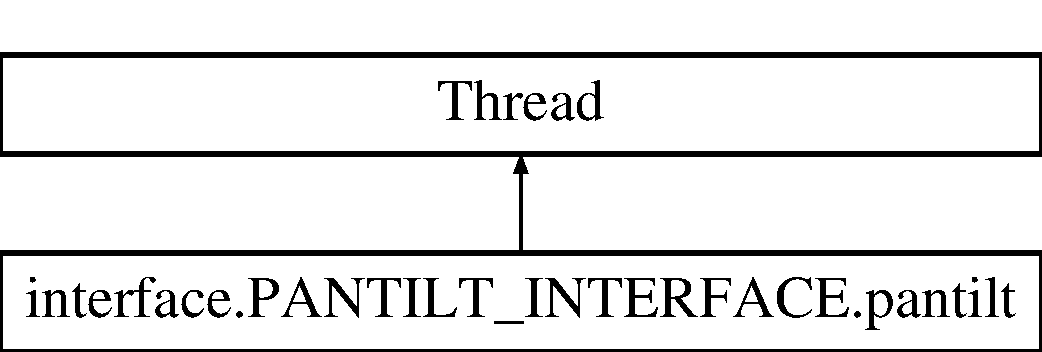
\includegraphics[height=2.000000cm]{classinterface_1_1PANTILT__INTERFACE_1_1pantilt}
\end{center}
\end{figure}
\subsection*{Public Member Functions}
\begin{DoxyCompactItemize}
\item 
def \hyperlink{classinterface_1_1PANTILT__INTERFACE_1_1pantilt_aa7d020e58aa179449247b1f13633fad5}{\+\_\+\+\_\+init\+\_\+\+\_\+}
\item 
def \hyperlink{classinterface_1_1PANTILT__INTERFACE_1_1pantilt_a392fb49d4df58462baeece46745f43f7}{run}
\end{DoxyCompactItemize}
\subsection*{Public Attributes}
\begin{DoxyCompactItemize}
\item 
\hyperlink{classinterface_1_1PANTILT__INTERFACE_1_1pantilt_a4442738a7ee24df1e8c6e95164ae9544}{parent}
\item 
\hyperlink{classinterface_1_1PANTILT__INTERFACE_1_1pantilt_a17986d3dabe0004cc86452d4d421059f}{num}
\item 
\hyperlink{classinterface_1_1PANTILT__INTERFACE_1_1pantilt_a77c1550064e91d0db075dea7c9aa9a90}{model}
\item 
\hyperlink{classinterface_1_1PANTILT__INTERFACE_1_1pantilt_a08bc9b59792cb71a7c7f167fd6ae5d85}{is\+Running}
\item 
\hyperlink{classinterface_1_1PANTILT__INTERFACE_1_1pantilt_a091704dbc6e8f320a8bf165627ddf915}{i2c}
\item 
\hyperlink{classinterface_1_1PANTILT__INTERFACE_1_1pantilt_a38bb4cf26d92df42d52715872377cdef}{controller}
\end{DoxyCompactItemize}


\subsection{Constructor \& Destructor Documentation}
\hypertarget{classinterface_1_1PANTILT__INTERFACE_1_1pantilt_aa7d020e58aa179449247b1f13633fad5}{}\index{interface\+::\+P\+A\+N\+T\+I\+L\+T\+\_\+\+I\+N\+T\+E\+R\+F\+A\+C\+E\+::pantilt@{interface\+::\+P\+A\+N\+T\+I\+L\+T\+\_\+\+I\+N\+T\+E\+R\+F\+A\+C\+E\+::pantilt}!\+\_\+\+\_\+init\+\_\+\+\_\+@{\+\_\+\+\_\+init\+\_\+\+\_\+}}
\index{\+\_\+\+\_\+init\+\_\+\+\_\+@{\+\_\+\+\_\+init\+\_\+\+\_\+}!interface\+::\+P\+A\+N\+T\+I\+L\+T\+\_\+\+I\+N\+T\+E\+R\+F\+A\+C\+E\+::pantilt@{interface\+::\+P\+A\+N\+T\+I\+L\+T\+\_\+\+I\+N\+T\+E\+R\+F\+A\+C\+E\+::pantilt}}
\subsubsection[{\+\_\+\+\_\+init\+\_\+\+\_\+}]{\setlength{\rightskip}{0pt plus 5cm}def interface.\+P\+A\+N\+T\+I\+L\+T\+\_\+\+I\+N\+T\+E\+R\+F\+A\+C\+E.\+pantilt.\+\_\+\+\_\+init\+\_\+\+\_\+ (
\begin{DoxyParamCaption}
\item[{}]{self}
\end{DoxyParamCaption}
)}\label{classinterface_1_1PANTILT__INTERFACE_1_1pantilt_aa7d020e58aa179449247b1f13633fad5}


\subsection{Member Function Documentation}
\hypertarget{classinterface_1_1PANTILT__INTERFACE_1_1pantilt_a392fb49d4df58462baeece46745f43f7}{}\index{interface\+::\+P\+A\+N\+T\+I\+L\+T\+\_\+\+I\+N\+T\+E\+R\+F\+A\+C\+E\+::pantilt@{interface\+::\+P\+A\+N\+T\+I\+L\+T\+\_\+\+I\+N\+T\+E\+R\+F\+A\+C\+E\+::pantilt}!run@{run}}
\index{run@{run}!interface\+::\+P\+A\+N\+T\+I\+L\+T\+\_\+\+I\+N\+T\+E\+R\+F\+A\+C\+E\+::pantilt@{interface\+::\+P\+A\+N\+T\+I\+L\+T\+\_\+\+I\+N\+T\+E\+R\+F\+A\+C\+E\+::pantilt}}
\subsubsection[{run}]{\setlength{\rightskip}{0pt plus 5cm}def interface.\+P\+A\+N\+T\+I\+L\+T\+\_\+\+I\+N\+T\+E\+R\+F\+A\+C\+E.\+pantilt.\+run (
\begin{DoxyParamCaption}
\item[{}]{self}
\end{DoxyParamCaption}
)}\label{classinterface_1_1PANTILT__INTERFACE_1_1pantilt_a392fb49d4df58462baeece46745f43f7}


\subsection{Member Data Documentation}
\hypertarget{classinterface_1_1PANTILT__INTERFACE_1_1pantilt_a38bb4cf26d92df42d52715872377cdef}{}\index{interface\+::\+P\+A\+N\+T\+I\+L\+T\+\_\+\+I\+N\+T\+E\+R\+F\+A\+C\+E\+::pantilt@{interface\+::\+P\+A\+N\+T\+I\+L\+T\+\_\+\+I\+N\+T\+E\+R\+F\+A\+C\+E\+::pantilt}!controller@{controller}}
\index{controller@{controller}!interface\+::\+P\+A\+N\+T\+I\+L\+T\+\_\+\+I\+N\+T\+E\+R\+F\+A\+C\+E\+::pantilt@{interface\+::\+P\+A\+N\+T\+I\+L\+T\+\_\+\+I\+N\+T\+E\+R\+F\+A\+C\+E\+::pantilt}}
\subsubsection[{controller}]{\setlength{\rightskip}{0pt plus 5cm}interface.\+P\+A\+N\+T\+I\+L\+T\+\_\+\+I\+N\+T\+E\+R\+F\+A\+C\+E.\+pantilt.\+controller}\label{classinterface_1_1PANTILT__INTERFACE_1_1pantilt_a38bb4cf26d92df42d52715872377cdef}
\hypertarget{classinterface_1_1PANTILT__INTERFACE_1_1pantilt_a091704dbc6e8f320a8bf165627ddf915}{}\index{interface\+::\+P\+A\+N\+T\+I\+L\+T\+\_\+\+I\+N\+T\+E\+R\+F\+A\+C\+E\+::pantilt@{interface\+::\+P\+A\+N\+T\+I\+L\+T\+\_\+\+I\+N\+T\+E\+R\+F\+A\+C\+E\+::pantilt}!i2c@{i2c}}
\index{i2c@{i2c}!interface\+::\+P\+A\+N\+T\+I\+L\+T\+\_\+\+I\+N\+T\+E\+R\+F\+A\+C\+E\+::pantilt@{interface\+::\+P\+A\+N\+T\+I\+L\+T\+\_\+\+I\+N\+T\+E\+R\+F\+A\+C\+E\+::pantilt}}
\subsubsection[{i2c}]{\setlength{\rightskip}{0pt plus 5cm}interface.\+P\+A\+N\+T\+I\+L\+T\+\_\+\+I\+N\+T\+E\+R\+F\+A\+C\+E.\+pantilt.\+i2c}\label{classinterface_1_1PANTILT__INTERFACE_1_1pantilt_a091704dbc6e8f320a8bf165627ddf915}
\hypertarget{classinterface_1_1PANTILT__INTERFACE_1_1pantilt_a08bc9b59792cb71a7c7f167fd6ae5d85}{}\index{interface\+::\+P\+A\+N\+T\+I\+L\+T\+\_\+\+I\+N\+T\+E\+R\+F\+A\+C\+E\+::pantilt@{interface\+::\+P\+A\+N\+T\+I\+L\+T\+\_\+\+I\+N\+T\+E\+R\+F\+A\+C\+E\+::pantilt}!is\+Running@{is\+Running}}
\index{is\+Running@{is\+Running}!interface\+::\+P\+A\+N\+T\+I\+L\+T\+\_\+\+I\+N\+T\+E\+R\+F\+A\+C\+E\+::pantilt@{interface\+::\+P\+A\+N\+T\+I\+L\+T\+\_\+\+I\+N\+T\+E\+R\+F\+A\+C\+E\+::pantilt}}
\subsubsection[{is\+Running}]{\setlength{\rightskip}{0pt plus 5cm}interface.\+P\+A\+N\+T\+I\+L\+T\+\_\+\+I\+N\+T\+E\+R\+F\+A\+C\+E.\+pantilt.\+is\+Running}\label{classinterface_1_1PANTILT__INTERFACE_1_1pantilt_a08bc9b59792cb71a7c7f167fd6ae5d85}
\hypertarget{classinterface_1_1PANTILT__INTERFACE_1_1pantilt_a77c1550064e91d0db075dea7c9aa9a90}{}\index{interface\+::\+P\+A\+N\+T\+I\+L\+T\+\_\+\+I\+N\+T\+E\+R\+F\+A\+C\+E\+::pantilt@{interface\+::\+P\+A\+N\+T\+I\+L\+T\+\_\+\+I\+N\+T\+E\+R\+F\+A\+C\+E\+::pantilt}!model@{model}}
\index{model@{model}!interface\+::\+P\+A\+N\+T\+I\+L\+T\+\_\+\+I\+N\+T\+E\+R\+F\+A\+C\+E\+::pantilt@{interface\+::\+P\+A\+N\+T\+I\+L\+T\+\_\+\+I\+N\+T\+E\+R\+F\+A\+C\+E\+::pantilt}}
\subsubsection[{model}]{\setlength{\rightskip}{0pt plus 5cm}interface.\+P\+A\+N\+T\+I\+L\+T\+\_\+\+I\+N\+T\+E\+R\+F\+A\+C\+E.\+pantilt.\+model}\label{classinterface_1_1PANTILT__INTERFACE_1_1pantilt_a77c1550064e91d0db075dea7c9aa9a90}
\hypertarget{classinterface_1_1PANTILT__INTERFACE_1_1pantilt_a17986d3dabe0004cc86452d4d421059f}{}\index{interface\+::\+P\+A\+N\+T\+I\+L\+T\+\_\+\+I\+N\+T\+E\+R\+F\+A\+C\+E\+::pantilt@{interface\+::\+P\+A\+N\+T\+I\+L\+T\+\_\+\+I\+N\+T\+E\+R\+F\+A\+C\+E\+::pantilt}!num@{num}}
\index{num@{num}!interface\+::\+P\+A\+N\+T\+I\+L\+T\+\_\+\+I\+N\+T\+E\+R\+F\+A\+C\+E\+::pantilt@{interface\+::\+P\+A\+N\+T\+I\+L\+T\+\_\+\+I\+N\+T\+E\+R\+F\+A\+C\+E\+::pantilt}}
\subsubsection[{num}]{\setlength{\rightskip}{0pt plus 5cm}interface.\+P\+A\+N\+T\+I\+L\+T\+\_\+\+I\+N\+T\+E\+R\+F\+A\+C\+E.\+pantilt.\+num}\label{classinterface_1_1PANTILT__INTERFACE_1_1pantilt_a17986d3dabe0004cc86452d4d421059f}
\hypertarget{classinterface_1_1PANTILT__INTERFACE_1_1pantilt_a4442738a7ee24df1e8c6e95164ae9544}{}\index{interface\+::\+P\+A\+N\+T\+I\+L\+T\+\_\+\+I\+N\+T\+E\+R\+F\+A\+C\+E\+::pantilt@{interface\+::\+P\+A\+N\+T\+I\+L\+T\+\_\+\+I\+N\+T\+E\+R\+F\+A\+C\+E\+::pantilt}!parent@{parent}}
\index{parent@{parent}!interface\+::\+P\+A\+N\+T\+I\+L\+T\+\_\+\+I\+N\+T\+E\+R\+F\+A\+C\+E\+::pantilt@{interface\+::\+P\+A\+N\+T\+I\+L\+T\+\_\+\+I\+N\+T\+E\+R\+F\+A\+C\+E\+::pantilt}}
\subsubsection[{parent}]{\setlength{\rightskip}{0pt plus 5cm}interface.\+P\+A\+N\+T\+I\+L\+T\+\_\+\+I\+N\+T\+E\+R\+F\+A\+C\+E.\+pantilt.\+parent}\label{classinterface_1_1PANTILT__INTERFACE_1_1pantilt_a4442738a7ee24df1e8c6e95164ae9544}


The documentation for this class was generated from the following file\+:\begin{DoxyCompactItemize}
\item 
interface/\hyperlink{PANTILT__INTERFACE_8py}{P\+A\+N\+T\+I\+L\+T\+\_\+\+I\+N\+T\+E\+R\+F\+A\+C\+E.\+py}\end{DoxyCompactItemize}

\hypertarget{classcontroller_1_1PANTILT__CONTROLLER_1_1pantilt}{}\section{controller.\+P\+A\+N\+T\+I\+L\+T\+\_\+\+C\+O\+N\+T\+R\+O\+L\+L\+E\+R.\+pantilt Class Reference}
\label{classcontroller_1_1PANTILT__CONTROLLER_1_1pantilt}\index{controller.\+P\+A\+N\+T\+I\+L\+T\+\_\+\+C\+O\+N\+T\+R\+O\+L\+L\+E\+R.\+pantilt@{controller.\+P\+A\+N\+T\+I\+L\+T\+\_\+\+C\+O\+N\+T\+R\+O\+L\+L\+E\+R.\+pantilt}}
Inheritance diagram for controller.\+P\+A\+N\+T\+I\+L\+T\+\_\+\+C\+O\+N\+T\+R\+O\+L\+L\+E\+R.\+pantilt\+:\begin{figure}[H]
\begin{center}
\leavevmode
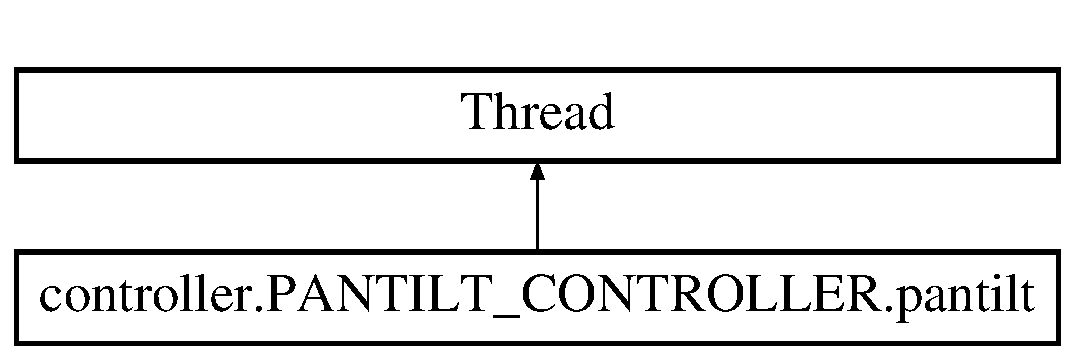
\includegraphics[height=2.000000cm]{classcontroller_1_1PANTILT__CONTROLLER_1_1pantilt}
\end{center}
\end{figure}
\subsection*{Public Member Functions}
\begin{DoxyCompactItemize}
\item 
def \hyperlink{classcontroller_1_1PANTILT__CONTROLLER_1_1pantilt_a7de0de26f776775e5f1f4f165eabad5a}{\+\_\+\+\_\+init\+\_\+\+\_\+}
\item 
def \hyperlink{classcontroller_1_1PANTILT__CONTROLLER_1_1pantilt_abdd9e553f5882fb024a18a02a23bdf85}{run}
\end{DoxyCompactItemize}
\subsection*{Public Attributes}
\begin{DoxyCompactItemize}
\item 
\hyperlink{classcontroller_1_1PANTILT__CONTROLLER_1_1pantilt_afc2fa0a554c0d3ec465bf09d832fcf54}{parent}
\item 
\hyperlink{classcontroller_1_1PANTILT__CONTROLLER_1_1pantilt_a15cf83499c83b96b5eee02601919438f}{num}
\item 
\hyperlink{classcontroller_1_1PANTILT__CONTROLLER_1_1pantilt_a0e92951db4608e830b4b37616aa41096}{is\+Running}
\item 
\hyperlink{classcontroller_1_1PANTILT__CONTROLLER_1_1pantilt_af5635593bc5a63d45be083aa5e165a65}{driver1}
\item 
\hyperlink{classcontroller_1_1PANTILT__CONTROLLER_1_1pantilt_addf843595361a7270e1917354c8d41f2}{model}
\item 
\hyperlink{classcontroller_1_1PANTILT__CONTROLLER_1_1pantilt_a4b09a9cbf7fac18361ae3e9a772c7585}{tilt\+\_\+servo}
\item 
\hyperlink{classcontroller_1_1PANTILT__CONTROLLER_1_1pantilt_a384533b87bffe38df020ed6bfc992817}{pan\+\_\+servo}
\end{DoxyCompactItemize}


\subsection{Constructor \& Destructor Documentation}
\hypertarget{classcontroller_1_1PANTILT__CONTROLLER_1_1pantilt_a7de0de26f776775e5f1f4f165eabad5a}{}\index{controller\+::\+P\+A\+N\+T\+I\+L\+T\+\_\+\+C\+O\+N\+T\+R\+O\+L\+L\+E\+R\+::pantilt@{controller\+::\+P\+A\+N\+T\+I\+L\+T\+\_\+\+C\+O\+N\+T\+R\+O\+L\+L\+E\+R\+::pantilt}!\+\_\+\+\_\+init\+\_\+\+\_\+@{\+\_\+\+\_\+init\+\_\+\+\_\+}}
\index{\+\_\+\+\_\+init\+\_\+\+\_\+@{\+\_\+\+\_\+init\+\_\+\+\_\+}!controller\+::\+P\+A\+N\+T\+I\+L\+T\+\_\+\+C\+O\+N\+T\+R\+O\+L\+L\+E\+R\+::pantilt@{controller\+::\+P\+A\+N\+T\+I\+L\+T\+\_\+\+C\+O\+N\+T\+R\+O\+L\+L\+E\+R\+::pantilt}}
\subsubsection[{\+\_\+\+\_\+init\+\_\+\+\_\+}]{\setlength{\rightskip}{0pt plus 5cm}def controller.\+P\+A\+N\+T\+I\+L\+T\+\_\+\+C\+O\+N\+T\+R\+O\+L\+L\+E\+R.\+pantilt.\+\_\+\+\_\+init\+\_\+\+\_\+ (
\begin{DoxyParamCaption}
\item[{}]{self, }
\item[{}]{M\+O\+D\+E\+L, }
\item[{}]{I2\+C}
\end{DoxyParamCaption}
)}\label{classcontroller_1_1PANTILT__CONTROLLER_1_1pantilt_a7de0de26f776775e5f1f4f165eabad5a}


\subsection{Member Function Documentation}
\hypertarget{classcontroller_1_1PANTILT__CONTROLLER_1_1pantilt_abdd9e553f5882fb024a18a02a23bdf85}{}\index{controller\+::\+P\+A\+N\+T\+I\+L\+T\+\_\+\+C\+O\+N\+T\+R\+O\+L\+L\+E\+R\+::pantilt@{controller\+::\+P\+A\+N\+T\+I\+L\+T\+\_\+\+C\+O\+N\+T\+R\+O\+L\+L\+E\+R\+::pantilt}!run@{run}}
\index{run@{run}!controller\+::\+P\+A\+N\+T\+I\+L\+T\+\_\+\+C\+O\+N\+T\+R\+O\+L\+L\+E\+R\+::pantilt@{controller\+::\+P\+A\+N\+T\+I\+L\+T\+\_\+\+C\+O\+N\+T\+R\+O\+L\+L\+E\+R\+::pantilt}}
\subsubsection[{run}]{\setlength{\rightskip}{0pt plus 5cm}def controller.\+P\+A\+N\+T\+I\+L\+T\+\_\+\+C\+O\+N\+T\+R\+O\+L\+L\+E\+R.\+pantilt.\+run (
\begin{DoxyParamCaption}
\item[{}]{self}
\end{DoxyParamCaption}
)}\label{classcontroller_1_1PANTILT__CONTROLLER_1_1pantilt_abdd9e553f5882fb024a18a02a23bdf85}


\subsection{Member Data Documentation}
\hypertarget{classcontroller_1_1PANTILT__CONTROLLER_1_1pantilt_af5635593bc5a63d45be083aa5e165a65}{}\index{controller\+::\+P\+A\+N\+T\+I\+L\+T\+\_\+\+C\+O\+N\+T\+R\+O\+L\+L\+E\+R\+::pantilt@{controller\+::\+P\+A\+N\+T\+I\+L\+T\+\_\+\+C\+O\+N\+T\+R\+O\+L\+L\+E\+R\+::pantilt}!driver1@{driver1}}
\index{driver1@{driver1}!controller\+::\+P\+A\+N\+T\+I\+L\+T\+\_\+\+C\+O\+N\+T\+R\+O\+L\+L\+E\+R\+::pantilt@{controller\+::\+P\+A\+N\+T\+I\+L\+T\+\_\+\+C\+O\+N\+T\+R\+O\+L\+L\+E\+R\+::pantilt}}
\subsubsection[{driver1}]{\setlength{\rightskip}{0pt plus 5cm}controller.\+P\+A\+N\+T\+I\+L\+T\+\_\+\+C\+O\+N\+T\+R\+O\+L\+L\+E\+R.\+pantilt.\+driver1}\label{classcontroller_1_1PANTILT__CONTROLLER_1_1pantilt_af5635593bc5a63d45be083aa5e165a65}
\hypertarget{classcontroller_1_1PANTILT__CONTROLLER_1_1pantilt_a0e92951db4608e830b4b37616aa41096}{}\index{controller\+::\+P\+A\+N\+T\+I\+L\+T\+\_\+\+C\+O\+N\+T\+R\+O\+L\+L\+E\+R\+::pantilt@{controller\+::\+P\+A\+N\+T\+I\+L\+T\+\_\+\+C\+O\+N\+T\+R\+O\+L\+L\+E\+R\+::pantilt}!is\+Running@{is\+Running}}
\index{is\+Running@{is\+Running}!controller\+::\+P\+A\+N\+T\+I\+L\+T\+\_\+\+C\+O\+N\+T\+R\+O\+L\+L\+E\+R\+::pantilt@{controller\+::\+P\+A\+N\+T\+I\+L\+T\+\_\+\+C\+O\+N\+T\+R\+O\+L\+L\+E\+R\+::pantilt}}
\subsubsection[{is\+Running}]{\setlength{\rightskip}{0pt plus 5cm}controller.\+P\+A\+N\+T\+I\+L\+T\+\_\+\+C\+O\+N\+T\+R\+O\+L\+L\+E\+R.\+pantilt.\+is\+Running}\label{classcontroller_1_1PANTILT__CONTROLLER_1_1pantilt_a0e92951db4608e830b4b37616aa41096}
\hypertarget{classcontroller_1_1PANTILT__CONTROLLER_1_1pantilt_addf843595361a7270e1917354c8d41f2}{}\index{controller\+::\+P\+A\+N\+T\+I\+L\+T\+\_\+\+C\+O\+N\+T\+R\+O\+L\+L\+E\+R\+::pantilt@{controller\+::\+P\+A\+N\+T\+I\+L\+T\+\_\+\+C\+O\+N\+T\+R\+O\+L\+L\+E\+R\+::pantilt}!model@{model}}
\index{model@{model}!controller\+::\+P\+A\+N\+T\+I\+L\+T\+\_\+\+C\+O\+N\+T\+R\+O\+L\+L\+E\+R\+::pantilt@{controller\+::\+P\+A\+N\+T\+I\+L\+T\+\_\+\+C\+O\+N\+T\+R\+O\+L\+L\+E\+R\+::pantilt}}
\subsubsection[{model}]{\setlength{\rightskip}{0pt plus 5cm}controller.\+P\+A\+N\+T\+I\+L\+T\+\_\+\+C\+O\+N\+T\+R\+O\+L\+L\+E\+R.\+pantilt.\+model}\label{classcontroller_1_1PANTILT__CONTROLLER_1_1pantilt_addf843595361a7270e1917354c8d41f2}
\hypertarget{classcontroller_1_1PANTILT__CONTROLLER_1_1pantilt_a15cf83499c83b96b5eee02601919438f}{}\index{controller\+::\+P\+A\+N\+T\+I\+L\+T\+\_\+\+C\+O\+N\+T\+R\+O\+L\+L\+E\+R\+::pantilt@{controller\+::\+P\+A\+N\+T\+I\+L\+T\+\_\+\+C\+O\+N\+T\+R\+O\+L\+L\+E\+R\+::pantilt}!num@{num}}
\index{num@{num}!controller\+::\+P\+A\+N\+T\+I\+L\+T\+\_\+\+C\+O\+N\+T\+R\+O\+L\+L\+E\+R\+::pantilt@{controller\+::\+P\+A\+N\+T\+I\+L\+T\+\_\+\+C\+O\+N\+T\+R\+O\+L\+L\+E\+R\+::pantilt}}
\subsubsection[{num}]{\setlength{\rightskip}{0pt plus 5cm}controller.\+P\+A\+N\+T\+I\+L\+T\+\_\+\+C\+O\+N\+T\+R\+O\+L\+L\+E\+R.\+pantilt.\+num}\label{classcontroller_1_1PANTILT__CONTROLLER_1_1pantilt_a15cf83499c83b96b5eee02601919438f}
\hypertarget{classcontroller_1_1PANTILT__CONTROLLER_1_1pantilt_a384533b87bffe38df020ed6bfc992817}{}\index{controller\+::\+P\+A\+N\+T\+I\+L\+T\+\_\+\+C\+O\+N\+T\+R\+O\+L\+L\+E\+R\+::pantilt@{controller\+::\+P\+A\+N\+T\+I\+L\+T\+\_\+\+C\+O\+N\+T\+R\+O\+L\+L\+E\+R\+::pantilt}!pan\+\_\+servo@{pan\+\_\+servo}}
\index{pan\+\_\+servo@{pan\+\_\+servo}!controller\+::\+P\+A\+N\+T\+I\+L\+T\+\_\+\+C\+O\+N\+T\+R\+O\+L\+L\+E\+R\+::pantilt@{controller\+::\+P\+A\+N\+T\+I\+L\+T\+\_\+\+C\+O\+N\+T\+R\+O\+L\+L\+E\+R\+::pantilt}}
\subsubsection[{pan\+\_\+servo}]{\setlength{\rightskip}{0pt plus 5cm}controller.\+P\+A\+N\+T\+I\+L\+T\+\_\+\+C\+O\+N\+T\+R\+O\+L\+L\+E\+R.\+pantilt.\+pan\+\_\+servo}\label{classcontroller_1_1PANTILT__CONTROLLER_1_1pantilt_a384533b87bffe38df020ed6bfc992817}
\hypertarget{classcontroller_1_1PANTILT__CONTROLLER_1_1pantilt_afc2fa0a554c0d3ec465bf09d832fcf54}{}\index{controller\+::\+P\+A\+N\+T\+I\+L\+T\+\_\+\+C\+O\+N\+T\+R\+O\+L\+L\+E\+R\+::pantilt@{controller\+::\+P\+A\+N\+T\+I\+L\+T\+\_\+\+C\+O\+N\+T\+R\+O\+L\+L\+E\+R\+::pantilt}!parent@{parent}}
\index{parent@{parent}!controller\+::\+P\+A\+N\+T\+I\+L\+T\+\_\+\+C\+O\+N\+T\+R\+O\+L\+L\+E\+R\+::pantilt@{controller\+::\+P\+A\+N\+T\+I\+L\+T\+\_\+\+C\+O\+N\+T\+R\+O\+L\+L\+E\+R\+::pantilt}}
\subsubsection[{parent}]{\setlength{\rightskip}{0pt plus 5cm}controller.\+P\+A\+N\+T\+I\+L\+T\+\_\+\+C\+O\+N\+T\+R\+O\+L\+L\+E\+R.\+pantilt.\+parent}\label{classcontroller_1_1PANTILT__CONTROLLER_1_1pantilt_afc2fa0a554c0d3ec465bf09d832fcf54}
\hypertarget{classcontroller_1_1PANTILT__CONTROLLER_1_1pantilt_a4b09a9cbf7fac18361ae3e9a772c7585}{}\index{controller\+::\+P\+A\+N\+T\+I\+L\+T\+\_\+\+C\+O\+N\+T\+R\+O\+L\+L\+E\+R\+::pantilt@{controller\+::\+P\+A\+N\+T\+I\+L\+T\+\_\+\+C\+O\+N\+T\+R\+O\+L\+L\+E\+R\+::pantilt}!tilt\+\_\+servo@{tilt\+\_\+servo}}
\index{tilt\+\_\+servo@{tilt\+\_\+servo}!controller\+::\+P\+A\+N\+T\+I\+L\+T\+\_\+\+C\+O\+N\+T\+R\+O\+L\+L\+E\+R\+::pantilt@{controller\+::\+P\+A\+N\+T\+I\+L\+T\+\_\+\+C\+O\+N\+T\+R\+O\+L\+L\+E\+R\+::pantilt}}
\subsubsection[{tilt\+\_\+servo}]{\setlength{\rightskip}{0pt plus 5cm}controller.\+P\+A\+N\+T\+I\+L\+T\+\_\+\+C\+O\+N\+T\+R\+O\+L\+L\+E\+R.\+pantilt.\+tilt\+\_\+servo}\label{classcontroller_1_1PANTILT__CONTROLLER_1_1pantilt_a4b09a9cbf7fac18361ae3e9a772c7585}


The documentation for this class was generated from the following file\+:\begin{DoxyCompactItemize}
\item 
controller/\hyperlink{PANTILT__CONTROLLER_8py}{P\+A\+N\+T\+I\+L\+T\+\_\+\+C\+O\+N\+T\+R\+O\+L\+L\+E\+R.\+py}\end{DoxyCompactItemize}

\hypertarget{classmodel_1_1PANTILT__MODEL_1_1pantilt}{}\section{model.\+P\+A\+N\+T\+I\+L\+T\+\_\+\+M\+O\+D\+E\+L.\+pantilt Class Reference}
\label{classmodel_1_1PANTILT__MODEL_1_1pantilt}\index{model.\+P\+A\+N\+T\+I\+L\+T\+\_\+\+M\+O\+D\+E\+L.\+pantilt@{model.\+P\+A\+N\+T\+I\+L\+T\+\_\+\+M\+O\+D\+E\+L.\+pantilt}}
\subsection*{Public Member Functions}
\begin{DoxyCompactItemize}
\item 
def \hyperlink{classmodel_1_1PANTILT__MODEL_1_1pantilt_a427ce8d85390b98a65fba754b394f37a}{\+\_\+\+\_\+init\+\_\+\+\_\+}
\end{DoxyCompactItemize}
\subsection*{Public Attributes}
\begin{DoxyCompactItemize}
\item 
\hyperlink{classmodel_1_1PANTILT__MODEL_1_1pantilt_a7833827d59e9bd6212b147b90ba923e7}{tilt\+\_\+angle}
\item 
\hyperlink{classmodel_1_1PANTILT__MODEL_1_1pantilt_a3c9ae4ae2bfb981b9258752f8baf9878}{pan\+\_\+angle}
\item 
\hyperlink{classmodel_1_1PANTILT__MODEL_1_1pantilt_abed248a0b87a8f060c65e185125cea09}{tilt\+\_\+min}
\item 
\hyperlink{classmodel_1_1PANTILT__MODEL_1_1pantilt_a774886c6a767076f047395c605e1262f}{tilt\+\_\+max}
\item 
\hyperlink{classmodel_1_1PANTILT__MODEL_1_1pantilt_adf70a2a96aab83f9a9557c0aae51bfbb}{pan\+\_\+min}
\item 
\hyperlink{classmodel_1_1PANTILT__MODEL_1_1pantilt_a1ba69acbc76ac90737dd509da61762be}{pan\+\_\+max}
\item 
\hyperlink{classmodel_1_1PANTILT__MODEL_1_1pantilt_ab0d3687530a05750330e616d8cd902b9}{tilt\+\_\+servo\+\_\+\+I\+D}
\item 
\hyperlink{classmodel_1_1PANTILT__MODEL_1_1pantilt_a3516dc36ca1b80a3fcd01f8a88cd4974}{mode}
\end{DoxyCompactItemize}


\subsection{Constructor \& Destructor Documentation}
\hypertarget{classmodel_1_1PANTILT__MODEL_1_1pantilt_a427ce8d85390b98a65fba754b394f37a}{}\index{model\+::\+P\+A\+N\+T\+I\+L\+T\+\_\+\+M\+O\+D\+E\+L\+::pantilt@{model\+::\+P\+A\+N\+T\+I\+L\+T\+\_\+\+M\+O\+D\+E\+L\+::pantilt}!\+\_\+\+\_\+init\+\_\+\+\_\+@{\+\_\+\+\_\+init\+\_\+\+\_\+}}
\index{\+\_\+\+\_\+init\+\_\+\+\_\+@{\+\_\+\+\_\+init\+\_\+\+\_\+}!model\+::\+P\+A\+N\+T\+I\+L\+T\+\_\+\+M\+O\+D\+E\+L\+::pantilt@{model\+::\+P\+A\+N\+T\+I\+L\+T\+\_\+\+M\+O\+D\+E\+L\+::pantilt}}
\subsubsection[{\+\_\+\+\_\+init\+\_\+\+\_\+}]{\setlength{\rightskip}{0pt plus 5cm}def model.\+P\+A\+N\+T\+I\+L\+T\+\_\+\+M\+O\+D\+E\+L.\+pantilt.\+\_\+\+\_\+init\+\_\+\+\_\+ (
\begin{DoxyParamCaption}
\item[{}]{self}
\end{DoxyParamCaption}
)}\label{classmodel_1_1PANTILT__MODEL_1_1pantilt_a427ce8d85390b98a65fba754b394f37a}


\subsection{Member Data Documentation}
\hypertarget{classmodel_1_1PANTILT__MODEL_1_1pantilt_a3516dc36ca1b80a3fcd01f8a88cd4974}{}\index{model\+::\+P\+A\+N\+T\+I\+L\+T\+\_\+\+M\+O\+D\+E\+L\+::pantilt@{model\+::\+P\+A\+N\+T\+I\+L\+T\+\_\+\+M\+O\+D\+E\+L\+::pantilt}!mode@{mode}}
\index{mode@{mode}!model\+::\+P\+A\+N\+T\+I\+L\+T\+\_\+\+M\+O\+D\+E\+L\+::pantilt@{model\+::\+P\+A\+N\+T\+I\+L\+T\+\_\+\+M\+O\+D\+E\+L\+::pantilt}}
\subsubsection[{mode}]{\setlength{\rightskip}{0pt plus 5cm}model.\+P\+A\+N\+T\+I\+L\+T\+\_\+\+M\+O\+D\+E\+L.\+pantilt.\+mode}\label{classmodel_1_1PANTILT__MODEL_1_1pantilt_a3516dc36ca1b80a3fcd01f8a88cd4974}
\hypertarget{classmodel_1_1PANTILT__MODEL_1_1pantilt_a3c9ae4ae2bfb981b9258752f8baf9878}{}\index{model\+::\+P\+A\+N\+T\+I\+L\+T\+\_\+\+M\+O\+D\+E\+L\+::pantilt@{model\+::\+P\+A\+N\+T\+I\+L\+T\+\_\+\+M\+O\+D\+E\+L\+::pantilt}!pan\+\_\+angle@{pan\+\_\+angle}}
\index{pan\+\_\+angle@{pan\+\_\+angle}!model\+::\+P\+A\+N\+T\+I\+L\+T\+\_\+\+M\+O\+D\+E\+L\+::pantilt@{model\+::\+P\+A\+N\+T\+I\+L\+T\+\_\+\+M\+O\+D\+E\+L\+::pantilt}}
\subsubsection[{pan\+\_\+angle}]{\setlength{\rightskip}{0pt plus 5cm}model.\+P\+A\+N\+T\+I\+L\+T\+\_\+\+M\+O\+D\+E\+L.\+pantilt.\+pan\+\_\+angle}\label{classmodel_1_1PANTILT__MODEL_1_1pantilt_a3c9ae4ae2bfb981b9258752f8baf9878}
\hypertarget{classmodel_1_1PANTILT__MODEL_1_1pantilt_a1ba69acbc76ac90737dd509da61762be}{}\index{model\+::\+P\+A\+N\+T\+I\+L\+T\+\_\+\+M\+O\+D\+E\+L\+::pantilt@{model\+::\+P\+A\+N\+T\+I\+L\+T\+\_\+\+M\+O\+D\+E\+L\+::pantilt}!pan\+\_\+max@{pan\+\_\+max}}
\index{pan\+\_\+max@{pan\+\_\+max}!model\+::\+P\+A\+N\+T\+I\+L\+T\+\_\+\+M\+O\+D\+E\+L\+::pantilt@{model\+::\+P\+A\+N\+T\+I\+L\+T\+\_\+\+M\+O\+D\+E\+L\+::pantilt}}
\subsubsection[{pan\+\_\+max}]{\setlength{\rightskip}{0pt plus 5cm}model.\+P\+A\+N\+T\+I\+L\+T\+\_\+\+M\+O\+D\+E\+L.\+pantilt.\+pan\+\_\+max}\label{classmodel_1_1PANTILT__MODEL_1_1pantilt_a1ba69acbc76ac90737dd509da61762be}
\hypertarget{classmodel_1_1PANTILT__MODEL_1_1pantilt_adf70a2a96aab83f9a9557c0aae51bfbb}{}\index{model\+::\+P\+A\+N\+T\+I\+L\+T\+\_\+\+M\+O\+D\+E\+L\+::pantilt@{model\+::\+P\+A\+N\+T\+I\+L\+T\+\_\+\+M\+O\+D\+E\+L\+::pantilt}!pan\+\_\+min@{pan\+\_\+min}}
\index{pan\+\_\+min@{pan\+\_\+min}!model\+::\+P\+A\+N\+T\+I\+L\+T\+\_\+\+M\+O\+D\+E\+L\+::pantilt@{model\+::\+P\+A\+N\+T\+I\+L\+T\+\_\+\+M\+O\+D\+E\+L\+::pantilt}}
\subsubsection[{pan\+\_\+min}]{\setlength{\rightskip}{0pt plus 5cm}model.\+P\+A\+N\+T\+I\+L\+T\+\_\+\+M\+O\+D\+E\+L.\+pantilt.\+pan\+\_\+min}\label{classmodel_1_1PANTILT__MODEL_1_1pantilt_adf70a2a96aab83f9a9557c0aae51bfbb}
\hypertarget{classmodel_1_1PANTILT__MODEL_1_1pantilt_a7833827d59e9bd6212b147b90ba923e7}{}\index{model\+::\+P\+A\+N\+T\+I\+L\+T\+\_\+\+M\+O\+D\+E\+L\+::pantilt@{model\+::\+P\+A\+N\+T\+I\+L\+T\+\_\+\+M\+O\+D\+E\+L\+::pantilt}!tilt\+\_\+angle@{tilt\+\_\+angle}}
\index{tilt\+\_\+angle@{tilt\+\_\+angle}!model\+::\+P\+A\+N\+T\+I\+L\+T\+\_\+\+M\+O\+D\+E\+L\+::pantilt@{model\+::\+P\+A\+N\+T\+I\+L\+T\+\_\+\+M\+O\+D\+E\+L\+::pantilt}}
\subsubsection[{tilt\+\_\+angle}]{\setlength{\rightskip}{0pt plus 5cm}model.\+P\+A\+N\+T\+I\+L\+T\+\_\+\+M\+O\+D\+E\+L.\+pantilt.\+tilt\+\_\+angle}\label{classmodel_1_1PANTILT__MODEL_1_1pantilt_a7833827d59e9bd6212b147b90ba923e7}
\hypertarget{classmodel_1_1PANTILT__MODEL_1_1pantilt_a774886c6a767076f047395c605e1262f}{}\index{model\+::\+P\+A\+N\+T\+I\+L\+T\+\_\+\+M\+O\+D\+E\+L\+::pantilt@{model\+::\+P\+A\+N\+T\+I\+L\+T\+\_\+\+M\+O\+D\+E\+L\+::pantilt}!tilt\+\_\+max@{tilt\+\_\+max}}
\index{tilt\+\_\+max@{tilt\+\_\+max}!model\+::\+P\+A\+N\+T\+I\+L\+T\+\_\+\+M\+O\+D\+E\+L\+::pantilt@{model\+::\+P\+A\+N\+T\+I\+L\+T\+\_\+\+M\+O\+D\+E\+L\+::pantilt}}
\subsubsection[{tilt\+\_\+max}]{\setlength{\rightskip}{0pt plus 5cm}model.\+P\+A\+N\+T\+I\+L\+T\+\_\+\+M\+O\+D\+E\+L.\+pantilt.\+tilt\+\_\+max}\label{classmodel_1_1PANTILT__MODEL_1_1pantilt_a774886c6a767076f047395c605e1262f}
\hypertarget{classmodel_1_1PANTILT__MODEL_1_1pantilt_abed248a0b87a8f060c65e185125cea09}{}\index{model\+::\+P\+A\+N\+T\+I\+L\+T\+\_\+\+M\+O\+D\+E\+L\+::pantilt@{model\+::\+P\+A\+N\+T\+I\+L\+T\+\_\+\+M\+O\+D\+E\+L\+::pantilt}!tilt\+\_\+min@{tilt\+\_\+min}}
\index{tilt\+\_\+min@{tilt\+\_\+min}!model\+::\+P\+A\+N\+T\+I\+L\+T\+\_\+\+M\+O\+D\+E\+L\+::pantilt@{model\+::\+P\+A\+N\+T\+I\+L\+T\+\_\+\+M\+O\+D\+E\+L\+::pantilt}}
\subsubsection[{tilt\+\_\+min}]{\setlength{\rightskip}{0pt plus 5cm}model.\+P\+A\+N\+T\+I\+L\+T\+\_\+\+M\+O\+D\+E\+L.\+pantilt.\+tilt\+\_\+min}\label{classmodel_1_1PANTILT__MODEL_1_1pantilt_abed248a0b87a8f060c65e185125cea09}
\hypertarget{classmodel_1_1PANTILT__MODEL_1_1pantilt_ab0d3687530a05750330e616d8cd902b9}{}\index{model\+::\+P\+A\+N\+T\+I\+L\+T\+\_\+\+M\+O\+D\+E\+L\+::pantilt@{model\+::\+P\+A\+N\+T\+I\+L\+T\+\_\+\+M\+O\+D\+E\+L\+::pantilt}!tilt\+\_\+servo\+\_\+\+I\+D@{tilt\+\_\+servo\+\_\+\+I\+D}}
\index{tilt\+\_\+servo\+\_\+\+I\+D@{tilt\+\_\+servo\+\_\+\+I\+D}!model\+::\+P\+A\+N\+T\+I\+L\+T\+\_\+\+M\+O\+D\+E\+L\+::pantilt@{model\+::\+P\+A\+N\+T\+I\+L\+T\+\_\+\+M\+O\+D\+E\+L\+::pantilt}}
\subsubsection[{tilt\+\_\+servo\+\_\+\+I\+D}]{\setlength{\rightskip}{0pt plus 5cm}model.\+P\+A\+N\+T\+I\+L\+T\+\_\+\+M\+O\+D\+E\+L.\+pantilt.\+tilt\+\_\+servo\+\_\+\+I\+D}\label{classmodel_1_1PANTILT__MODEL_1_1pantilt_ab0d3687530a05750330e616d8cd902b9}


The documentation for this class was generated from the following file\+:\begin{DoxyCompactItemize}
\item 
model/\hyperlink{PANTILT__MODEL_8py}{P\+A\+N\+T\+I\+L\+T\+\_\+\+M\+O\+D\+E\+L.\+py}\end{DoxyCompactItemize}

\hypertarget{classdriver_1_1DRIVER__CORE_1_1PCA9865}{}\section{driver.\+D\+R\+I\+V\+E\+R\+\_\+\+C\+O\+R\+E.\+P\+C\+A9865 Class Reference}
\label{classdriver_1_1DRIVER__CORE_1_1PCA9865}\index{driver.\+D\+R\+I\+V\+E\+R\+\_\+\+C\+O\+R\+E.\+P\+C\+A9865@{driver.\+D\+R\+I\+V\+E\+R\+\_\+\+C\+O\+R\+E.\+P\+C\+A9865}}
\subsection*{Public Member Functions}
\begin{DoxyCompactItemize}
\item 
def \hyperlink{classdriver_1_1DRIVER__CORE_1_1PCA9865_ae727575a3372b8b4d90ffa314081c489}{\+\_\+\+\_\+init\+\_\+\+\_\+}
\item 
def \hyperlink{classdriver_1_1DRIVER__CORE_1_1PCA9865_a425edd2aa5693f5fea64d0aec65f77e8}{set\+Freq}
\item 
def \hyperlink{classdriver_1_1DRIVER__CORE_1_1PCA9865_a2482e9c19788095bfc47ebdb62b4903d}{\+\_\+\+\_\+calc\+\_\+prescale\+\_\+\+\_\+}
\item 
def \hyperlink{classdriver_1_1DRIVER__CORE_1_1PCA9865_ae727575a3372b8b4d90ffa314081c489}{\+\_\+\+\_\+init\+\_\+\+\_\+}
\item 
def \hyperlink{classdriver_1_1DRIVER__CORE_1_1PCA9865_a425edd2aa5693f5fea64d0aec65f77e8}{set\+Freq}
\item 
def \hyperlink{classdriver_1_1DRIVER__CORE_1_1PCA9865_a2482e9c19788095bfc47ebdb62b4903d}{\+\_\+\+\_\+calc\+\_\+prescale\+\_\+\+\_\+}
\item 
def \hyperlink{classdriver_1_1DRIVER__CORE_1_1PCA9865_ae727575a3372b8b4d90ffa314081c489}{\+\_\+\+\_\+init\+\_\+\+\_\+}
\item 
def \hyperlink{classdriver_1_1DRIVER__CORE_1_1PCA9865_a425edd2aa5693f5fea64d0aec65f77e8}{set\+Freq}
\item 
def \hyperlink{classdriver_1_1DRIVER__CORE_1_1PCA9865_a2482e9c19788095bfc47ebdb62b4903d}{\+\_\+\+\_\+calc\+\_\+prescale\+\_\+\+\_\+}
\item 
def \hyperlink{classdriver_1_1DRIVER__CORE_1_1PCA9865_ae727575a3372b8b4d90ffa314081c489}{\+\_\+\+\_\+init\+\_\+\+\_\+}
\item 
def \hyperlink{classdriver_1_1DRIVER__CORE_1_1PCA9865_a425edd2aa5693f5fea64d0aec65f77e8}{set\+Freq}
\item 
def \hyperlink{classdriver_1_1DRIVER__CORE_1_1PCA9865_a2482e9c19788095bfc47ebdb62b4903d}{\+\_\+\+\_\+calc\+\_\+prescale\+\_\+\+\_\+}
\end{DoxyCompactItemize}
\subsection*{Public Attributes}
\begin{DoxyCompactItemize}
\item 
\hyperlink{classdriver_1_1DRIVER__CORE_1_1PCA9865_a3a4b2748c61f79822d6602c941535bd2}{i2c}
\end{DoxyCompactItemize}
\subsection*{Static Public Attributes}
\begin{DoxyCompactItemize}
\item 
int \hyperlink{classdriver_1_1DRIVER__CORE_1_1PCA9865_ad9aef9648195aa00f5ae496992073930}{F\+R\+E\+Q\+\_\+\+M\+I\+N} = 50
\item 
int \hyperlink{classdriver_1_1DRIVER__CORE_1_1PCA9865_a5394eec714130c246fe47c35a2af683a}{F\+R\+E\+Q\+\_\+\+M\+A\+X} = 300
\end{DoxyCompactItemize}


\subsection{Constructor \& Destructor Documentation}
\hypertarget{classdriver_1_1DRIVER__CORE_1_1PCA9865_ae727575a3372b8b4d90ffa314081c489}{}\index{driver\+::\+D\+R\+I\+V\+E\+R\+\_\+\+C\+O\+R\+E\+::\+P\+C\+A9865@{driver\+::\+D\+R\+I\+V\+E\+R\+\_\+\+C\+O\+R\+E\+::\+P\+C\+A9865}!\+\_\+\+\_\+init\+\_\+\+\_\+@{\+\_\+\+\_\+init\+\_\+\+\_\+}}
\index{\+\_\+\+\_\+init\+\_\+\+\_\+@{\+\_\+\+\_\+init\+\_\+\+\_\+}!driver\+::\+D\+R\+I\+V\+E\+R\+\_\+\+C\+O\+R\+E\+::\+P\+C\+A9865@{driver\+::\+D\+R\+I\+V\+E\+R\+\_\+\+C\+O\+R\+E\+::\+P\+C\+A9865}}
\subsubsection[{\+\_\+\+\_\+init\+\_\+\+\_\+}]{\setlength{\rightskip}{0pt plus 5cm}def driver.\+D\+R\+I\+V\+E\+R\+\_\+\+C\+O\+R\+E.\+P\+C\+A9865.\+\_\+\+\_\+init\+\_\+\+\_\+ (
\begin{DoxyParamCaption}
\item[{}]{self, }
\item[{}]{port, }
\item[{}]{busnum = {\ttfamily -\/1}, }
\item[{}]{debug = {\ttfamily False}}
\end{DoxyParamCaption}
)}\label{classdriver_1_1DRIVER__CORE_1_1PCA9865_ae727575a3372b8b4d90ffa314081c489}
\begin{DoxyVerb}When creating driver objects the port for the device must be specified. Ports are integers values from 1 - 2. Returns nothing.
\end{DoxyVerb}
 \hypertarget{classdriver_1_1DRIVER__CORE_1_1PCA9865_ae727575a3372b8b4d90ffa314081c489}{}\index{driver\+::\+D\+R\+I\+V\+E\+R\+\_\+\+C\+O\+R\+E\+::\+P\+C\+A9865@{driver\+::\+D\+R\+I\+V\+E\+R\+\_\+\+C\+O\+R\+E\+::\+P\+C\+A9865}!\+\_\+\+\_\+init\+\_\+\+\_\+@{\+\_\+\+\_\+init\+\_\+\+\_\+}}
\index{\+\_\+\+\_\+init\+\_\+\+\_\+@{\+\_\+\+\_\+init\+\_\+\+\_\+}!driver\+::\+D\+R\+I\+V\+E\+R\+\_\+\+C\+O\+R\+E\+::\+P\+C\+A9865@{driver\+::\+D\+R\+I\+V\+E\+R\+\_\+\+C\+O\+R\+E\+::\+P\+C\+A9865}}
\subsubsection[{\+\_\+\+\_\+init\+\_\+\+\_\+}]{\setlength{\rightskip}{0pt plus 5cm}def driver.\+D\+R\+I\+V\+E\+R\+\_\+\+C\+O\+R\+E.\+P\+C\+A9865.\+\_\+\+\_\+init\+\_\+\+\_\+ (
\begin{DoxyParamCaption}
\item[{}]{self, }
\item[{}]{port, }
\item[{}]{busnum = {\ttfamily -\/1}, }
\item[{}]{debug = {\ttfamily False}}
\end{DoxyParamCaption}
)}\label{classdriver_1_1DRIVER__CORE_1_1PCA9865_ae727575a3372b8b4d90ffa314081c489}
\begin{DoxyVerb}When creating driver objects the port for the device must be specified. Ports are integers values from 1 - 2. Returns nothing.
\end{DoxyVerb}
 \hypertarget{classdriver_1_1DRIVER__CORE_1_1PCA9865_ae727575a3372b8b4d90ffa314081c489}{}\index{driver\+::\+D\+R\+I\+V\+E\+R\+\_\+\+C\+O\+R\+E\+::\+P\+C\+A9865@{driver\+::\+D\+R\+I\+V\+E\+R\+\_\+\+C\+O\+R\+E\+::\+P\+C\+A9865}!\+\_\+\+\_\+init\+\_\+\+\_\+@{\+\_\+\+\_\+init\+\_\+\+\_\+}}
\index{\+\_\+\+\_\+init\+\_\+\+\_\+@{\+\_\+\+\_\+init\+\_\+\+\_\+}!driver\+::\+D\+R\+I\+V\+E\+R\+\_\+\+C\+O\+R\+E\+::\+P\+C\+A9865@{driver\+::\+D\+R\+I\+V\+E\+R\+\_\+\+C\+O\+R\+E\+::\+P\+C\+A9865}}
\subsubsection[{\+\_\+\+\_\+init\+\_\+\+\_\+}]{\setlength{\rightskip}{0pt plus 5cm}def driver.\+D\+R\+I\+V\+E\+R\+\_\+\+C\+O\+R\+E.\+P\+C\+A9865.\+\_\+\+\_\+init\+\_\+\+\_\+ (
\begin{DoxyParamCaption}
\item[{}]{self, }
\item[{}]{port, }
\item[{}]{busnum = {\ttfamily -\/1}, }
\item[{}]{debug = {\ttfamily False}}
\end{DoxyParamCaption}
)}\label{classdriver_1_1DRIVER__CORE_1_1PCA9865_ae727575a3372b8b4d90ffa314081c489}
\begin{DoxyVerb}When creating driver objects the port for the device must be specified. Ports are integers values from 1 - 2. Returns nothing.
\end{DoxyVerb}
 \hypertarget{classdriver_1_1DRIVER__CORE_1_1PCA9865_ae727575a3372b8b4d90ffa314081c489}{}\index{driver\+::\+D\+R\+I\+V\+E\+R\+\_\+\+C\+O\+R\+E\+::\+P\+C\+A9865@{driver\+::\+D\+R\+I\+V\+E\+R\+\_\+\+C\+O\+R\+E\+::\+P\+C\+A9865}!\+\_\+\+\_\+init\+\_\+\+\_\+@{\+\_\+\+\_\+init\+\_\+\+\_\+}}
\index{\+\_\+\+\_\+init\+\_\+\+\_\+@{\+\_\+\+\_\+init\+\_\+\+\_\+}!driver\+::\+D\+R\+I\+V\+E\+R\+\_\+\+C\+O\+R\+E\+::\+P\+C\+A9865@{driver\+::\+D\+R\+I\+V\+E\+R\+\_\+\+C\+O\+R\+E\+::\+P\+C\+A9865}}
\subsubsection[{\+\_\+\+\_\+init\+\_\+\+\_\+}]{\setlength{\rightskip}{0pt plus 5cm}def driver.\+D\+R\+I\+V\+E\+R\+\_\+\+C\+O\+R\+E.\+P\+C\+A9865.\+\_\+\+\_\+init\+\_\+\+\_\+ (
\begin{DoxyParamCaption}
\item[{}]{self, }
\item[{}]{port, }
\item[{}]{busnum = {\ttfamily -\/1}, }
\item[{}]{debug = {\ttfamily False}}
\end{DoxyParamCaption}
)}\label{classdriver_1_1DRIVER__CORE_1_1PCA9865_ae727575a3372b8b4d90ffa314081c489}
\begin{DoxyVerb}When creating driver objects the port for the device must be specified. Ports are integers values from 1 - 2. Returns nothing.
\end{DoxyVerb}
 

\subsection{Member Function Documentation}
\hypertarget{classdriver_1_1DRIVER__CORE_1_1PCA9865_a2482e9c19788095bfc47ebdb62b4903d}{}\index{driver\+::\+D\+R\+I\+V\+E\+R\+\_\+\+C\+O\+R\+E\+::\+P\+C\+A9865@{driver\+::\+D\+R\+I\+V\+E\+R\+\_\+\+C\+O\+R\+E\+::\+P\+C\+A9865}!\+\_\+\+\_\+calc\+\_\+prescale\+\_\+\+\_\+@{\+\_\+\+\_\+calc\+\_\+prescale\+\_\+\+\_\+}}
\index{\+\_\+\+\_\+calc\+\_\+prescale\+\_\+\+\_\+@{\+\_\+\+\_\+calc\+\_\+prescale\+\_\+\+\_\+}!driver\+::\+D\+R\+I\+V\+E\+R\+\_\+\+C\+O\+R\+E\+::\+P\+C\+A9865@{driver\+::\+D\+R\+I\+V\+E\+R\+\_\+\+C\+O\+R\+E\+::\+P\+C\+A9865}}
\subsubsection[{\+\_\+\+\_\+calc\+\_\+prescale\+\_\+\+\_\+}]{\setlength{\rightskip}{0pt plus 5cm}def driver.\+D\+R\+I\+V\+E\+R\+\_\+\+C\+O\+R\+E.\+P\+C\+A9865.\+\_\+\+\_\+calc\+\_\+prescale\+\_\+\+\_\+ (
\begin{DoxyParamCaption}
\item[{}]{self, }
\item[{}]{freq}
\end{DoxyParamCaption}
)}\label{classdriver_1_1DRIVER__CORE_1_1PCA9865_a2482e9c19788095bfc47ebdb62b4903d}
\begin{DoxyVerb}Converts the input frequency into the appropriate values for the PCA9865 driver. See PCA9865 datasheet for more information.
\end{DoxyVerb}
 \hypertarget{classdriver_1_1DRIVER__CORE_1_1PCA9865_a2482e9c19788095bfc47ebdb62b4903d}{}\index{driver\+::\+D\+R\+I\+V\+E\+R\+\_\+\+C\+O\+R\+E\+::\+P\+C\+A9865@{driver\+::\+D\+R\+I\+V\+E\+R\+\_\+\+C\+O\+R\+E\+::\+P\+C\+A9865}!\+\_\+\+\_\+calc\+\_\+prescale\+\_\+\+\_\+@{\+\_\+\+\_\+calc\+\_\+prescale\+\_\+\+\_\+}}
\index{\+\_\+\+\_\+calc\+\_\+prescale\+\_\+\+\_\+@{\+\_\+\+\_\+calc\+\_\+prescale\+\_\+\+\_\+}!driver\+::\+D\+R\+I\+V\+E\+R\+\_\+\+C\+O\+R\+E\+::\+P\+C\+A9865@{driver\+::\+D\+R\+I\+V\+E\+R\+\_\+\+C\+O\+R\+E\+::\+P\+C\+A9865}}
\subsubsection[{\+\_\+\+\_\+calc\+\_\+prescale\+\_\+\+\_\+}]{\setlength{\rightskip}{0pt plus 5cm}def driver.\+D\+R\+I\+V\+E\+R\+\_\+\+C\+O\+R\+E.\+P\+C\+A9865.\+\_\+\+\_\+calc\+\_\+prescale\+\_\+\+\_\+ (
\begin{DoxyParamCaption}
\item[{}]{self, }
\item[{}]{freq}
\end{DoxyParamCaption}
)}\label{classdriver_1_1DRIVER__CORE_1_1PCA9865_a2482e9c19788095bfc47ebdb62b4903d}
\begin{DoxyVerb}Converts the input frequency into the appropriate values for the PCA9865 driver. See PCA9865 datasheet for more information.
\end{DoxyVerb}
 \hypertarget{classdriver_1_1DRIVER__CORE_1_1PCA9865_a2482e9c19788095bfc47ebdb62b4903d}{}\index{driver\+::\+D\+R\+I\+V\+E\+R\+\_\+\+C\+O\+R\+E\+::\+P\+C\+A9865@{driver\+::\+D\+R\+I\+V\+E\+R\+\_\+\+C\+O\+R\+E\+::\+P\+C\+A9865}!\+\_\+\+\_\+calc\+\_\+prescale\+\_\+\+\_\+@{\+\_\+\+\_\+calc\+\_\+prescale\+\_\+\+\_\+}}
\index{\+\_\+\+\_\+calc\+\_\+prescale\+\_\+\+\_\+@{\+\_\+\+\_\+calc\+\_\+prescale\+\_\+\+\_\+}!driver\+::\+D\+R\+I\+V\+E\+R\+\_\+\+C\+O\+R\+E\+::\+P\+C\+A9865@{driver\+::\+D\+R\+I\+V\+E\+R\+\_\+\+C\+O\+R\+E\+::\+P\+C\+A9865}}
\subsubsection[{\+\_\+\+\_\+calc\+\_\+prescale\+\_\+\+\_\+}]{\setlength{\rightskip}{0pt plus 5cm}def driver.\+D\+R\+I\+V\+E\+R\+\_\+\+C\+O\+R\+E.\+P\+C\+A9865.\+\_\+\+\_\+calc\+\_\+prescale\+\_\+\+\_\+ (
\begin{DoxyParamCaption}
\item[{}]{self, }
\item[{}]{freq}
\end{DoxyParamCaption}
)}\label{classdriver_1_1DRIVER__CORE_1_1PCA9865_a2482e9c19788095bfc47ebdb62b4903d}
\begin{DoxyVerb}Converts the input frequency into the appropriate values for the PCA9865 driver. See PCA9865 datasheet for more information.
\end{DoxyVerb}
 \hypertarget{classdriver_1_1DRIVER__CORE_1_1PCA9865_a2482e9c19788095bfc47ebdb62b4903d}{}\index{driver\+::\+D\+R\+I\+V\+E\+R\+\_\+\+C\+O\+R\+E\+::\+P\+C\+A9865@{driver\+::\+D\+R\+I\+V\+E\+R\+\_\+\+C\+O\+R\+E\+::\+P\+C\+A9865}!\+\_\+\+\_\+calc\+\_\+prescale\+\_\+\+\_\+@{\+\_\+\+\_\+calc\+\_\+prescale\+\_\+\+\_\+}}
\index{\+\_\+\+\_\+calc\+\_\+prescale\+\_\+\+\_\+@{\+\_\+\+\_\+calc\+\_\+prescale\+\_\+\+\_\+}!driver\+::\+D\+R\+I\+V\+E\+R\+\_\+\+C\+O\+R\+E\+::\+P\+C\+A9865@{driver\+::\+D\+R\+I\+V\+E\+R\+\_\+\+C\+O\+R\+E\+::\+P\+C\+A9865}}
\subsubsection[{\+\_\+\+\_\+calc\+\_\+prescale\+\_\+\+\_\+}]{\setlength{\rightskip}{0pt plus 5cm}def driver.\+D\+R\+I\+V\+E\+R\+\_\+\+C\+O\+R\+E.\+P\+C\+A9865.\+\_\+\+\_\+calc\+\_\+prescale\+\_\+\+\_\+ (
\begin{DoxyParamCaption}
\item[{}]{self, }
\item[{}]{freq}
\end{DoxyParamCaption}
)}\label{classdriver_1_1DRIVER__CORE_1_1PCA9865_a2482e9c19788095bfc47ebdb62b4903d}
\begin{DoxyVerb}Converts the input frequency into the appropriate values for the PCA9865 driver. See PCA9865 datasheet for more information.
\end{DoxyVerb}
 \hypertarget{classdriver_1_1DRIVER__CORE_1_1PCA9865_a425edd2aa5693f5fea64d0aec65f77e8}{}\index{driver\+::\+D\+R\+I\+V\+E\+R\+\_\+\+C\+O\+R\+E\+::\+P\+C\+A9865@{driver\+::\+D\+R\+I\+V\+E\+R\+\_\+\+C\+O\+R\+E\+::\+P\+C\+A9865}!set\+Freq@{set\+Freq}}
\index{set\+Freq@{set\+Freq}!driver\+::\+D\+R\+I\+V\+E\+R\+\_\+\+C\+O\+R\+E\+::\+P\+C\+A9865@{driver\+::\+D\+R\+I\+V\+E\+R\+\_\+\+C\+O\+R\+E\+::\+P\+C\+A9865}}
\subsubsection[{set\+Freq}]{\setlength{\rightskip}{0pt plus 5cm}def driver.\+D\+R\+I\+V\+E\+R\+\_\+\+C\+O\+R\+E.\+P\+C\+A9865.\+set\+Freq (
\begin{DoxyParamCaption}
\item[{}]{self, }
\item[{}]{freq}
\end{DoxyParamCaption}
)}\label{classdriver_1_1DRIVER__CORE_1_1PCA9865_a425edd2aa5693f5fea64d0aec65f77e8}
\begin{DoxyVerb}Sets the oscillator frequency for the PCA9865 driver. Frequency values from 50 to 300 are allowed.
\end{DoxyVerb}
 \hypertarget{classdriver_1_1DRIVER__CORE_1_1PCA9865_a425edd2aa5693f5fea64d0aec65f77e8}{}\index{driver\+::\+D\+R\+I\+V\+E\+R\+\_\+\+C\+O\+R\+E\+::\+P\+C\+A9865@{driver\+::\+D\+R\+I\+V\+E\+R\+\_\+\+C\+O\+R\+E\+::\+P\+C\+A9865}!set\+Freq@{set\+Freq}}
\index{set\+Freq@{set\+Freq}!driver\+::\+D\+R\+I\+V\+E\+R\+\_\+\+C\+O\+R\+E\+::\+P\+C\+A9865@{driver\+::\+D\+R\+I\+V\+E\+R\+\_\+\+C\+O\+R\+E\+::\+P\+C\+A9865}}
\subsubsection[{set\+Freq}]{\setlength{\rightskip}{0pt plus 5cm}def driver.\+D\+R\+I\+V\+E\+R\+\_\+\+C\+O\+R\+E.\+P\+C\+A9865.\+set\+Freq (
\begin{DoxyParamCaption}
\item[{}]{self, }
\item[{}]{freq}
\end{DoxyParamCaption}
)}\label{classdriver_1_1DRIVER__CORE_1_1PCA9865_a425edd2aa5693f5fea64d0aec65f77e8}
\begin{DoxyVerb}Sets the oscillator frequency for the PCA9865 driver. Frequency values from 50 to 300 are allowed.
\end{DoxyVerb}
 \hypertarget{classdriver_1_1DRIVER__CORE_1_1PCA9865_a425edd2aa5693f5fea64d0aec65f77e8}{}\index{driver\+::\+D\+R\+I\+V\+E\+R\+\_\+\+C\+O\+R\+E\+::\+P\+C\+A9865@{driver\+::\+D\+R\+I\+V\+E\+R\+\_\+\+C\+O\+R\+E\+::\+P\+C\+A9865}!set\+Freq@{set\+Freq}}
\index{set\+Freq@{set\+Freq}!driver\+::\+D\+R\+I\+V\+E\+R\+\_\+\+C\+O\+R\+E\+::\+P\+C\+A9865@{driver\+::\+D\+R\+I\+V\+E\+R\+\_\+\+C\+O\+R\+E\+::\+P\+C\+A9865}}
\subsubsection[{set\+Freq}]{\setlength{\rightskip}{0pt plus 5cm}def driver.\+D\+R\+I\+V\+E\+R\+\_\+\+C\+O\+R\+E.\+P\+C\+A9865.\+set\+Freq (
\begin{DoxyParamCaption}
\item[{}]{self, }
\item[{}]{freq}
\end{DoxyParamCaption}
)}\label{classdriver_1_1DRIVER__CORE_1_1PCA9865_a425edd2aa5693f5fea64d0aec65f77e8}
\begin{DoxyVerb}Sets the oscillator frequency for the PCA9865 driver. Frequency values from 50 to 300 are allowed.
\end{DoxyVerb}
 \hypertarget{classdriver_1_1DRIVER__CORE_1_1PCA9865_a425edd2aa5693f5fea64d0aec65f77e8}{}\index{driver\+::\+D\+R\+I\+V\+E\+R\+\_\+\+C\+O\+R\+E\+::\+P\+C\+A9865@{driver\+::\+D\+R\+I\+V\+E\+R\+\_\+\+C\+O\+R\+E\+::\+P\+C\+A9865}!set\+Freq@{set\+Freq}}
\index{set\+Freq@{set\+Freq}!driver\+::\+D\+R\+I\+V\+E\+R\+\_\+\+C\+O\+R\+E\+::\+P\+C\+A9865@{driver\+::\+D\+R\+I\+V\+E\+R\+\_\+\+C\+O\+R\+E\+::\+P\+C\+A9865}}
\subsubsection[{set\+Freq}]{\setlength{\rightskip}{0pt plus 5cm}def driver.\+D\+R\+I\+V\+E\+R\+\_\+\+C\+O\+R\+E.\+P\+C\+A9865.\+set\+Freq (
\begin{DoxyParamCaption}
\item[{}]{self, }
\item[{}]{freq}
\end{DoxyParamCaption}
)}\label{classdriver_1_1DRIVER__CORE_1_1PCA9865_a425edd2aa5693f5fea64d0aec65f77e8}
\begin{DoxyVerb}Sets the oscillator frequency for the PCA9865 driver. Frequency values from 50 to 300 are allowed.
\end{DoxyVerb}
 

\subsection{Member Data Documentation}
\hypertarget{classdriver_1_1DRIVER__CORE_1_1PCA9865_a5394eec714130c246fe47c35a2af683a}{}\index{driver\+::\+D\+R\+I\+V\+E\+R\+\_\+\+C\+O\+R\+E\+::\+P\+C\+A9865@{driver\+::\+D\+R\+I\+V\+E\+R\+\_\+\+C\+O\+R\+E\+::\+P\+C\+A9865}!F\+R\+E\+Q\+\_\+\+M\+A\+X@{F\+R\+E\+Q\+\_\+\+M\+A\+X}}
\index{F\+R\+E\+Q\+\_\+\+M\+A\+X@{F\+R\+E\+Q\+\_\+\+M\+A\+X}!driver\+::\+D\+R\+I\+V\+E\+R\+\_\+\+C\+O\+R\+E\+::\+P\+C\+A9865@{driver\+::\+D\+R\+I\+V\+E\+R\+\_\+\+C\+O\+R\+E\+::\+P\+C\+A9865}}
\subsubsection[{F\+R\+E\+Q\+\_\+\+M\+A\+X}]{\setlength{\rightskip}{0pt plus 5cm}int driver.\+D\+R\+I\+V\+E\+R\+\_\+\+C\+O\+R\+E.\+P\+C\+A9865.\+F\+R\+E\+Q\+\_\+\+M\+A\+X = 300\hspace{0.3cm}{\ttfamily [static]}}\label{classdriver_1_1DRIVER__CORE_1_1PCA9865_a5394eec714130c246fe47c35a2af683a}
\hypertarget{classdriver_1_1DRIVER__CORE_1_1PCA9865_ad9aef9648195aa00f5ae496992073930}{}\index{driver\+::\+D\+R\+I\+V\+E\+R\+\_\+\+C\+O\+R\+E\+::\+P\+C\+A9865@{driver\+::\+D\+R\+I\+V\+E\+R\+\_\+\+C\+O\+R\+E\+::\+P\+C\+A9865}!F\+R\+E\+Q\+\_\+\+M\+I\+N@{F\+R\+E\+Q\+\_\+\+M\+I\+N}}
\index{F\+R\+E\+Q\+\_\+\+M\+I\+N@{F\+R\+E\+Q\+\_\+\+M\+I\+N}!driver\+::\+D\+R\+I\+V\+E\+R\+\_\+\+C\+O\+R\+E\+::\+P\+C\+A9865@{driver\+::\+D\+R\+I\+V\+E\+R\+\_\+\+C\+O\+R\+E\+::\+P\+C\+A9865}}
\subsubsection[{F\+R\+E\+Q\+\_\+\+M\+I\+N}]{\setlength{\rightskip}{0pt plus 5cm}int driver.\+D\+R\+I\+V\+E\+R\+\_\+\+C\+O\+R\+E.\+P\+C\+A9865.\+F\+R\+E\+Q\+\_\+\+M\+I\+N = 50\hspace{0.3cm}{\ttfamily [static]}}\label{classdriver_1_1DRIVER__CORE_1_1PCA9865_ad9aef9648195aa00f5ae496992073930}
\hypertarget{classdriver_1_1DRIVER__CORE_1_1PCA9865_a3a4b2748c61f79822d6602c941535bd2}{}\index{driver\+::\+D\+R\+I\+V\+E\+R\+\_\+\+C\+O\+R\+E\+::\+P\+C\+A9865@{driver\+::\+D\+R\+I\+V\+E\+R\+\_\+\+C\+O\+R\+E\+::\+P\+C\+A9865}!i2c@{i2c}}
\index{i2c@{i2c}!driver\+::\+D\+R\+I\+V\+E\+R\+\_\+\+C\+O\+R\+E\+::\+P\+C\+A9865@{driver\+::\+D\+R\+I\+V\+E\+R\+\_\+\+C\+O\+R\+E\+::\+P\+C\+A9865}}
\subsubsection[{i2c}]{\setlength{\rightskip}{0pt plus 5cm}driver.\+D\+R\+I\+V\+E\+R\+\_\+\+C\+O\+R\+E.\+P\+C\+A9865.\+i2c}\label{classdriver_1_1DRIVER__CORE_1_1PCA9865_a3a4b2748c61f79822d6602c941535bd2}


The documentation for this class was generated from the following file\+:\begin{DoxyCompactItemize}
\item 
build/lib.\+linux-\/x86\+\_\+64-\/2.\+7/driver/\hyperlink{build_2lib_8linux-x86__64-2_87_2driver_2DRIVER__CORE_8py}{D\+R\+I\+V\+E\+R\+\_\+\+C\+O\+R\+E.\+py}\end{DoxyCompactItemize}

\hypertarget{classnetwork_1_1NETWORK__CORE_1_1protocol}{}\section{network.\+N\+E\+T\+W\+O\+R\+K\+\_\+\+C\+O\+R\+E.\+protocol Class Reference}
\label{classnetwork_1_1NETWORK__CORE_1_1protocol}\index{network.\+N\+E\+T\+W\+O\+R\+K\+\_\+\+C\+O\+R\+E.\+protocol@{network.\+N\+E\+T\+W\+O\+R\+K\+\_\+\+C\+O\+R\+E.\+protocol}}
Inheritance diagram for network.\+N\+E\+T\+W\+O\+R\+K\+\_\+\+C\+O\+R\+E.\+protocol\+:\begin{figure}[H]
\begin{center}
\leavevmode
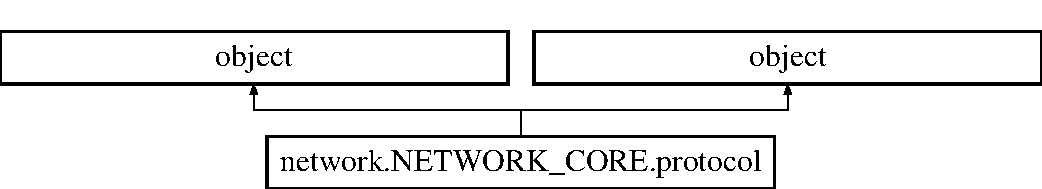
\includegraphics[height=2.000000cm]{classnetwork_1_1NETWORK__CORE_1_1protocol}
\end{center}
\end{figure}
\subsection*{Public Member Functions}
\begin{DoxyCompactItemize}
\item 
def \hyperlink{classnetwork_1_1NETWORK__CORE_1_1protocol_a1754de4b9a84dd46742631cdf072b993}{\+\_\+\+\_\+init\+\_\+\+\_\+}
\item 
def \hyperlink{classnetwork_1_1NETWORK__CORE_1_1protocol_a22c7d1bdfecc7b95f22def27922a6a16}{is\+Format}
\item 
def \hyperlink{classnetwork_1_1NETWORK__CORE_1_1protocol_ae949ee38090c3c7f80aec9a232571fd4}{parse}
\item 
def \hyperlink{classnetwork_1_1NETWORK__CORE_1_1protocol_a1754de4b9a84dd46742631cdf072b993}{\+\_\+\+\_\+init\+\_\+\+\_\+}
\item 
def \hyperlink{classnetwork_1_1NETWORK__CORE_1_1protocol_a22c7d1bdfecc7b95f22def27922a6a16}{is\+Format}
\item 
def \hyperlink{classnetwork_1_1NETWORK__CORE_1_1protocol_ae949ee38090c3c7f80aec9a232571fd4}{parse}
\end{DoxyCompactItemize}
\subsection*{Public Attributes}
\begin{DoxyCompactItemize}
\item 
\hyperlink{classnetwork_1_1NETWORK__CORE_1_1protocol_a1909533ebbc06331e4f698e614fe12db}{name}
\end{DoxyCompactItemize}


\subsection{Constructor \& Destructor Documentation}
\hypertarget{classnetwork_1_1NETWORK__CORE_1_1protocol_a1754de4b9a84dd46742631cdf072b993}{}\index{network\+::\+N\+E\+T\+W\+O\+R\+K\+\_\+\+C\+O\+R\+E\+::protocol@{network\+::\+N\+E\+T\+W\+O\+R\+K\+\_\+\+C\+O\+R\+E\+::protocol}!\+\_\+\+\_\+init\+\_\+\+\_\+@{\+\_\+\+\_\+init\+\_\+\+\_\+}}
\index{\+\_\+\+\_\+init\+\_\+\+\_\+@{\+\_\+\+\_\+init\+\_\+\+\_\+}!network\+::\+N\+E\+T\+W\+O\+R\+K\+\_\+\+C\+O\+R\+E\+::protocol@{network\+::\+N\+E\+T\+W\+O\+R\+K\+\_\+\+C\+O\+R\+E\+::protocol}}
\subsubsection[{\+\_\+\+\_\+init\+\_\+\+\_\+}]{\setlength{\rightskip}{0pt plus 5cm}def network.\+N\+E\+T\+W\+O\+R\+K\+\_\+\+C\+O\+R\+E.\+protocol.\+\_\+\+\_\+init\+\_\+\+\_\+ (
\begin{DoxyParamCaption}
\item[{}]{self, }
\item[{}]{name}
\end{DoxyParamCaption}
)}\label{classnetwork_1_1NETWORK__CORE_1_1protocol_a1754de4b9a84dd46742631cdf072b993}
\hypertarget{classnetwork_1_1NETWORK__CORE_1_1protocol_a1754de4b9a84dd46742631cdf072b993}{}\index{network\+::\+N\+E\+T\+W\+O\+R\+K\+\_\+\+C\+O\+R\+E\+::protocol@{network\+::\+N\+E\+T\+W\+O\+R\+K\+\_\+\+C\+O\+R\+E\+::protocol}!\+\_\+\+\_\+init\+\_\+\+\_\+@{\+\_\+\+\_\+init\+\_\+\+\_\+}}
\index{\+\_\+\+\_\+init\+\_\+\+\_\+@{\+\_\+\+\_\+init\+\_\+\+\_\+}!network\+::\+N\+E\+T\+W\+O\+R\+K\+\_\+\+C\+O\+R\+E\+::protocol@{network\+::\+N\+E\+T\+W\+O\+R\+K\+\_\+\+C\+O\+R\+E\+::protocol}}
\subsubsection[{\+\_\+\+\_\+init\+\_\+\+\_\+}]{\setlength{\rightskip}{0pt plus 5cm}def network.\+N\+E\+T\+W\+O\+R\+K\+\_\+\+C\+O\+R\+E.\+protocol.\+\_\+\+\_\+init\+\_\+\+\_\+ (
\begin{DoxyParamCaption}
\item[{}]{self, }
\item[{}]{name}
\end{DoxyParamCaption}
)}\label{classnetwork_1_1NETWORK__CORE_1_1protocol_a1754de4b9a84dd46742631cdf072b993}


\subsection{Member Function Documentation}
\hypertarget{classnetwork_1_1NETWORK__CORE_1_1protocol_a22c7d1bdfecc7b95f22def27922a6a16}{}\index{network\+::\+N\+E\+T\+W\+O\+R\+K\+\_\+\+C\+O\+R\+E\+::protocol@{network\+::\+N\+E\+T\+W\+O\+R\+K\+\_\+\+C\+O\+R\+E\+::protocol}!is\+Format@{is\+Format}}
\index{is\+Format@{is\+Format}!network\+::\+N\+E\+T\+W\+O\+R\+K\+\_\+\+C\+O\+R\+E\+::protocol@{network\+::\+N\+E\+T\+W\+O\+R\+K\+\_\+\+C\+O\+R\+E\+::protocol}}
\subsubsection[{is\+Format}]{\setlength{\rightskip}{0pt plus 5cm}def network.\+N\+E\+T\+W\+O\+R\+K\+\_\+\+C\+O\+R\+E.\+protocol.\+is\+Format (
\begin{DoxyParamCaption}
\item[{}]{self, }
\item[{}]{msg}
\end{DoxyParamCaption}
)}\label{classnetwork_1_1NETWORK__CORE_1_1protocol_a22c7d1bdfecc7b95f22def27922a6a16}
\hypertarget{classnetwork_1_1NETWORK__CORE_1_1protocol_a22c7d1bdfecc7b95f22def27922a6a16}{}\index{network\+::\+N\+E\+T\+W\+O\+R\+K\+\_\+\+C\+O\+R\+E\+::protocol@{network\+::\+N\+E\+T\+W\+O\+R\+K\+\_\+\+C\+O\+R\+E\+::protocol}!is\+Format@{is\+Format}}
\index{is\+Format@{is\+Format}!network\+::\+N\+E\+T\+W\+O\+R\+K\+\_\+\+C\+O\+R\+E\+::protocol@{network\+::\+N\+E\+T\+W\+O\+R\+K\+\_\+\+C\+O\+R\+E\+::protocol}}
\subsubsection[{is\+Format}]{\setlength{\rightskip}{0pt plus 5cm}def network.\+N\+E\+T\+W\+O\+R\+K\+\_\+\+C\+O\+R\+E.\+protocol.\+is\+Format (
\begin{DoxyParamCaption}
\item[{}]{self, }
\item[{}]{msg}
\end{DoxyParamCaption}
)}\label{classnetwork_1_1NETWORK__CORE_1_1protocol_a22c7d1bdfecc7b95f22def27922a6a16}
\hypertarget{classnetwork_1_1NETWORK__CORE_1_1protocol_ae949ee38090c3c7f80aec9a232571fd4}{}\index{network\+::\+N\+E\+T\+W\+O\+R\+K\+\_\+\+C\+O\+R\+E\+::protocol@{network\+::\+N\+E\+T\+W\+O\+R\+K\+\_\+\+C\+O\+R\+E\+::protocol}!parse@{parse}}
\index{parse@{parse}!network\+::\+N\+E\+T\+W\+O\+R\+K\+\_\+\+C\+O\+R\+E\+::protocol@{network\+::\+N\+E\+T\+W\+O\+R\+K\+\_\+\+C\+O\+R\+E\+::protocol}}
\subsubsection[{parse}]{\setlength{\rightskip}{0pt plus 5cm}def network.\+N\+E\+T\+W\+O\+R\+K\+\_\+\+C\+O\+R\+E.\+protocol.\+parse (
\begin{DoxyParamCaption}
\item[{}]{self, }
\item[{}]{msg}
\end{DoxyParamCaption}
)}\label{classnetwork_1_1NETWORK__CORE_1_1protocol_ae949ee38090c3c7f80aec9a232571fd4}
\hypertarget{classnetwork_1_1NETWORK__CORE_1_1protocol_ae949ee38090c3c7f80aec9a232571fd4}{}\index{network\+::\+N\+E\+T\+W\+O\+R\+K\+\_\+\+C\+O\+R\+E\+::protocol@{network\+::\+N\+E\+T\+W\+O\+R\+K\+\_\+\+C\+O\+R\+E\+::protocol}!parse@{parse}}
\index{parse@{parse}!network\+::\+N\+E\+T\+W\+O\+R\+K\+\_\+\+C\+O\+R\+E\+::protocol@{network\+::\+N\+E\+T\+W\+O\+R\+K\+\_\+\+C\+O\+R\+E\+::protocol}}
\subsubsection[{parse}]{\setlength{\rightskip}{0pt plus 5cm}def network.\+N\+E\+T\+W\+O\+R\+K\+\_\+\+C\+O\+R\+E.\+protocol.\+parse (
\begin{DoxyParamCaption}
\item[{}]{self, }
\item[{}]{msg}
\end{DoxyParamCaption}
)}\label{classnetwork_1_1NETWORK__CORE_1_1protocol_ae949ee38090c3c7f80aec9a232571fd4}


\subsection{Member Data Documentation}
\hypertarget{classnetwork_1_1NETWORK__CORE_1_1protocol_a1909533ebbc06331e4f698e614fe12db}{}\index{network\+::\+N\+E\+T\+W\+O\+R\+K\+\_\+\+C\+O\+R\+E\+::protocol@{network\+::\+N\+E\+T\+W\+O\+R\+K\+\_\+\+C\+O\+R\+E\+::protocol}!name@{name}}
\index{name@{name}!network\+::\+N\+E\+T\+W\+O\+R\+K\+\_\+\+C\+O\+R\+E\+::protocol@{network\+::\+N\+E\+T\+W\+O\+R\+K\+\_\+\+C\+O\+R\+E\+::protocol}}
\subsubsection[{name}]{\setlength{\rightskip}{0pt plus 5cm}network.\+N\+E\+T\+W\+O\+R\+K\+\_\+\+C\+O\+R\+E.\+protocol.\+name}\label{classnetwork_1_1NETWORK__CORE_1_1protocol_a1909533ebbc06331e4f698e614fe12db}


The documentation for this class was generated from the following file\+:\begin{DoxyCompactItemize}
\item 
build/lib.\+linux-\/x86\+\_\+64-\/2.\+7/network/\hyperlink{build_2lib_8linux-x86__64-2_87_2network_2NETWORK__CORE_8py}{N\+E\+T\+W\+O\+R\+K\+\_\+\+C\+O\+R\+E.\+py}\end{DoxyCompactItemize}

\hypertarget{classnetwork_1_1commsChannel_1_1UDPChannel}{}\section{network.\+comms\+Channel.\+U\+D\+P\+Channel Class Reference}
\label{classnetwork_1_1commsChannel_1_1UDPChannel}\index{network.\+comms\+Channel.\+U\+D\+P\+Channel@{network.\+comms\+Channel.\+U\+D\+P\+Channel}}
Inheritance diagram for network.\+comms\+Channel.\+U\+D\+P\+Channel\+:\begin{figure}[H]
\begin{center}
\leavevmode
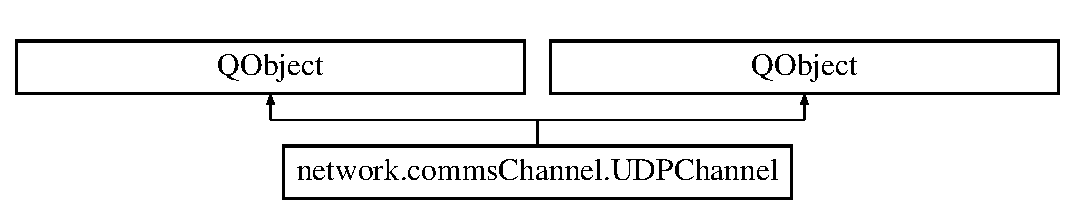
\includegraphics[height=1.222707cm]{classnetwork_1_1commsChannel_1_1UDPChannel}
\end{center}
\end{figure}
\subsection*{Public Member Functions}
\begin{DoxyCompactItemize}
\item 
def \hyperlink{classnetwork_1_1commsChannel_1_1UDPChannel_ae3e90f5c66765ae3f5d97334bb9767ad}{\+\_\+\+\_\+init\+\_\+\+\_\+}
\item 
def \hyperlink{classnetwork_1_1commsChannel_1_1UDPChannel_a7aeb7a38b3072fab11df4881fb22dd67}{send}
\item 
def \hyperlink{classnetwork_1_1commsChannel_1_1UDPChannel_a7aeb7a38b3072fab11df4881fb22dd67}{send}
\item 
def \hyperlink{classnetwork_1_1commsChannel_1_1UDPChannel_aeeda07b7e78ec0750501ca40d114aadc}{recv}
\item 
def \hyperlink{classnetwork_1_1commsChannel_1_1UDPChannel_a0e4df6f6b2e9030f6b58a945ab15e71d}{receive\+Function}
\item 
def \hyperlink{classnetwork_1_1commsChannel_1_1UDPChannel_a1a31b8bce874232ee25a022fe8a358dc}{start\+Recv}
\item 
def \hyperlink{classnetwork_1_1commsChannel_1_1UDPChannel_aa3eb1e0f39dbf4a9fed075600b104772}{stop\+Recv}
\item 
def \hyperlink{classnetwork_1_1commsChannel_1_1UDPChannel_ae3e90f5c66765ae3f5d97334bb9767ad}{\+\_\+\+\_\+init\+\_\+\+\_\+}
\item 
def \hyperlink{classnetwork_1_1commsChannel_1_1UDPChannel_a7aeb7a38b3072fab11df4881fb22dd67}{send}
\item 
def \hyperlink{classnetwork_1_1commsChannel_1_1UDPChannel_a7aeb7a38b3072fab11df4881fb22dd67}{send}
\item 
def \hyperlink{classnetwork_1_1commsChannel_1_1UDPChannel_aeeda07b7e78ec0750501ca40d114aadc}{recv}
\item 
def \hyperlink{classnetwork_1_1commsChannel_1_1UDPChannel_a0e4df6f6b2e9030f6b58a945ab15e71d}{receive\+Function}
\item 
def \hyperlink{classnetwork_1_1commsChannel_1_1UDPChannel_a1a31b8bce874232ee25a022fe8a358dc}{start\+Recv}
\item 
def \hyperlink{classnetwork_1_1commsChannel_1_1UDPChannel_aa3eb1e0f39dbf4a9fed075600b104772}{stop\+Recv}
\item 
def \hyperlink{classnetwork_1_1commsChannel_1_1UDPChannel_ae3e90f5c66765ae3f5d97334bb9767ad}{\+\_\+\+\_\+init\+\_\+\+\_\+}
\item 
def \hyperlink{classnetwork_1_1commsChannel_1_1UDPChannel_a7aeb7a38b3072fab11df4881fb22dd67}{send}
\item 
def \hyperlink{classnetwork_1_1commsChannel_1_1UDPChannel_a7aeb7a38b3072fab11df4881fb22dd67}{send}
\item 
def \hyperlink{classnetwork_1_1commsChannel_1_1UDPChannel_aeeda07b7e78ec0750501ca40d114aadc}{recv}
\item 
def \hyperlink{classnetwork_1_1commsChannel_1_1UDPChannel_a0e4df6f6b2e9030f6b58a945ab15e71d}{receive\+Function}
\item 
def \hyperlink{classnetwork_1_1commsChannel_1_1UDPChannel_a1a31b8bce874232ee25a022fe8a358dc}{start\+Recv}
\item 
def \hyperlink{classnetwork_1_1commsChannel_1_1UDPChannel_aa3eb1e0f39dbf4a9fed075600b104772}{stop\+Recv}
\item 
def \hyperlink{classnetwork_1_1commsChannel_1_1UDPChannel_ae3e90f5c66765ae3f5d97334bb9767ad}{\+\_\+\+\_\+init\+\_\+\+\_\+}
\item 
def \hyperlink{classnetwork_1_1commsChannel_1_1UDPChannel_a7aeb7a38b3072fab11df4881fb22dd67}{send}
\item 
def \hyperlink{classnetwork_1_1commsChannel_1_1UDPChannel_a7aeb7a38b3072fab11df4881fb22dd67}{send}
\item 
def \hyperlink{classnetwork_1_1commsChannel_1_1UDPChannel_aeeda07b7e78ec0750501ca40d114aadc}{recv}
\item 
def \hyperlink{classnetwork_1_1commsChannel_1_1UDPChannel_a0e4df6f6b2e9030f6b58a945ab15e71d}{receive\+Function}
\item 
def \hyperlink{classnetwork_1_1commsChannel_1_1UDPChannel_a1a31b8bce874232ee25a022fe8a358dc}{start\+Recv}
\item 
def \hyperlink{classnetwork_1_1commsChannel_1_1UDPChannel_aa3eb1e0f39dbf4a9fed075600b104772}{stop\+Recv}
\end{DoxyCompactItemize}
\subsection*{Public Attributes}
\begin{DoxyCompactItemize}
\item 
\hyperlink{classnetwork_1_1commsChannel_1_1UDPChannel_af43851623627900a93360187e7a4b5a0}{num}
\item 
\hyperlink{classnetwork_1_1commsChannel_1_1UDPChannel_a13939ef9b0ba434e2bb786d19f450b48}{ip}
\item 
\hyperlink{classnetwork_1_1commsChannel_1_1UDPChannel_a6b1a61243c41a625092986e6b38959e9}{port}
\item 
\hyperlink{classnetwork_1_1commsChannel_1_1UDPChannel_a19e4c1af17dc22d1c378ac53280fe679}{sock}
\item 
\hyperlink{classnetwork_1_1commsChannel_1_1UDPChannel_a8def8c5020988707811a671264d3b8b7}{thread}
\end{DoxyCompactItemize}
\subsection*{Static Public Attributes}
\begin{DoxyCompactItemize}
\item 
tuple \hyperlink{classnetwork_1_1commsChannel_1_1UDPChannel_ae1f826ff9e1f0eda9f4ef7127da5512b}{recv\+Event} = Qt\+Core.\+pyqt\+Signal(int, str,tuple)
\end{DoxyCompactItemize}


\subsection{Constructor \& Destructor Documentation}
\hypertarget{classnetwork_1_1commsChannel_1_1UDPChannel_ae3e90f5c66765ae3f5d97334bb9767ad}{}\index{network\+::comms\+Channel\+::\+U\+D\+P\+Channel@{network\+::comms\+Channel\+::\+U\+D\+P\+Channel}!\+\_\+\+\_\+init\+\_\+\+\_\+@{\+\_\+\+\_\+init\+\_\+\+\_\+}}
\index{\+\_\+\+\_\+init\+\_\+\+\_\+@{\+\_\+\+\_\+init\+\_\+\+\_\+}!network\+::comms\+Channel\+::\+U\+D\+P\+Channel@{network\+::comms\+Channel\+::\+U\+D\+P\+Channel}}
\subsubsection[{\+\_\+\+\_\+init\+\_\+\+\_\+}]{\setlength{\rightskip}{0pt plus 5cm}def network.\+comms\+Channel.\+U\+D\+P\+Channel.\+\_\+\+\_\+init\+\_\+\+\_\+ (
\begin{DoxyParamCaption}
\item[{}]{self, }
\item[{}]{num, }
\item[{}]{ip, }
\item[{}]{port, }
\item[{}]{timeout = {\ttfamily 1}}
\end{DoxyParamCaption}
)}\label{classnetwork_1_1commsChannel_1_1UDPChannel_ae3e90f5c66765ae3f5d97334bb9767ad}
\hypertarget{classnetwork_1_1commsChannel_1_1UDPChannel_ae3e90f5c66765ae3f5d97334bb9767ad}{}\index{network\+::comms\+Channel\+::\+U\+D\+P\+Channel@{network\+::comms\+Channel\+::\+U\+D\+P\+Channel}!\+\_\+\+\_\+init\+\_\+\+\_\+@{\+\_\+\+\_\+init\+\_\+\+\_\+}}
\index{\+\_\+\+\_\+init\+\_\+\+\_\+@{\+\_\+\+\_\+init\+\_\+\+\_\+}!network\+::comms\+Channel\+::\+U\+D\+P\+Channel@{network\+::comms\+Channel\+::\+U\+D\+P\+Channel}}
\subsubsection[{\+\_\+\+\_\+init\+\_\+\+\_\+}]{\setlength{\rightskip}{0pt plus 5cm}def network.\+comms\+Channel.\+U\+D\+P\+Channel.\+\_\+\+\_\+init\+\_\+\+\_\+ (
\begin{DoxyParamCaption}
\item[{}]{self, }
\item[{}]{num, }
\item[{}]{ip, }
\item[{}]{port, }
\item[{}]{timeout = {\ttfamily 1}}
\end{DoxyParamCaption}
)}\label{classnetwork_1_1commsChannel_1_1UDPChannel_ae3e90f5c66765ae3f5d97334bb9767ad}
\hypertarget{classnetwork_1_1commsChannel_1_1UDPChannel_ae3e90f5c66765ae3f5d97334bb9767ad}{}\index{network\+::comms\+Channel\+::\+U\+D\+P\+Channel@{network\+::comms\+Channel\+::\+U\+D\+P\+Channel}!\+\_\+\+\_\+init\+\_\+\+\_\+@{\+\_\+\+\_\+init\+\_\+\+\_\+}}
\index{\+\_\+\+\_\+init\+\_\+\+\_\+@{\+\_\+\+\_\+init\+\_\+\+\_\+}!network\+::comms\+Channel\+::\+U\+D\+P\+Channel@{network\+::comms\+Channel\+::\+U\+D\+P\+Channel}}
\subsubsection[{\+\_\+\+\_\+init\+\_\+\+\_\+}]{\setlength{\rightskip}{0pt plus 5cm}def network.\+comms\+Channel.\+U\+D\+P\+Channel.\+\_\+\+\_\+init\+\_\+\+\_\+ (
\begin{DoxyParamCaption}
\item[{}]{self, }
\item[{}]{num, }
\item[{}]{ip, }
\item[{}]{port, }
\item[{}]{timeout = {\ttfamily 1}}
\end{DoxyParamCaption}
)}\label{classnetwork_1_1commsChannel_1_1UDPChannel_ae3e90f5c66765ae3f5d97334bb9767ad}
\hypertarget{classnetwork_1_1commsChannel_1_1UDPChannel_ae3e90f5c66765ae3f5d97334bb9767ad}{}\index{network\+::comms\+Channel\+::\+U\+D\+P\+Channel@{network\+::comms\+Channel\+::\+U\+D\+P\+Channel}!\+\_\+\+\_\+init\+\_\+\+\_\+@{\+\_\+\+\_\+init\+\_\+\+\_\+}}
\index{\+\_\+\+\_\+init\+\_\+\+\_\+@{\+\_\+\+\_\+init\+\_\+\+\_\+}!network\+::comms\+Channel\+::\+U\+D\+P\+Channel@{network\+::comms\+Channel\+::\+U\+D\+P\+Channel}}
\subsubsection[{\+\_\+\+\_\+init\+\_\+\+\_\+}]{\setlength{\rightskip}{0pt plus 5cm}def network.\+comms\+Channel.\+U\+D\+P\+Channel.\+\_\+\+\_\+init\+\_\+\+\_\+ (
\begin{DoxyParamCaption}
\item[{}]{self, }
\item[{}]{num, }
\item[{}]{ip, }
\item[{}]{port, }
\item[{}]{timeout = {\ttfamily 1}}
\end{DoxyParamCaption}
)}\label{classnetwork_1_1commsChannel_1_1UDPChannel_ae3e90f5c66765ae3f5d97334bb9767ad}


\subsection{Member Function Documentation}
\hypertarget{classnetwork_1_1commsChannel_1_1UDPChannel_a0e4df6f6b2e9030f6b58a945ab15e71d}{}\index{network\+::comms\+Channel\+::\+U\+D\+P\+Channel@{network\+::comms\+Channel\+::\+U\+D\+P\+Channel}!receive\+Function@{receive\+Function}}
\index{receive\+Function@{receive\+Function}!network\+::comms\+Channel\+::\+U\+D\+P\+Channel@{network\+::comms\+Channel\+::\+U\+D\+P\+Channel}}
\subsubsection[{receive\+Function}]{\setlength{\rightskip}{0pt plus 5cm}def network.\+comms\+Channel.\+U\+D\+P\+Channel.\+receive\+Function (
\begin{DoxyParamCaption}
\item[{}]{self, }
\item[{}]{funct}
\end{DoxyParamCaption}
)}\label{classnetwork_1_1commsChannel_1_1UDPChannel_a0e4df6f6b2e9030f6b58a945ab15e71d}
\hypertarget{classnetwork_1_1commsChannel_1_1UDPChannel_a0e4df6f6b2e9030f6b58a945ab15e71d}{}\index{network\+::comms\+Channel\+::\+U\+D\+P\+Channel@{network\+::comms\+Channel\+::\+U\+D\+P\+Channel}!receive\+Function@{receive\+Function}}
\index{receive\+Function@{receive\+Function}!network\+::comms\+Channel\+::\+U\+D\+P\+Channel@{network\+::comms\+Channel\+::\+U\+D\+P\+Channel}}
\subsubsection[{receive\+Function}]{\setlength{\rightskip}{0pt plus 5cm}def network.\+comms\+Channel.\+U\+D\+P\+Channel.\+receive\+Function (
\begin{DoxyParamCaption}
\item[{}]{self, }
\item[{}]{funct}
\end{DoxyParamCaption}
)}\label{classnetwork_1_1commsChannel_1_1UDPChannel_a0e4df6f6b2e9030f6b58a945ab15e71d}
\hypertarget{classnetwork_1_1commsChannel_1_1UDPChannel_a0e4df6f6b2e9030f6b58a945ab15e71d}{}\index{network\+::comms\+Channel\+::\+U\+D\+P\+Channel@{network\+::comms\+Channel\+::\+U\+D\+P\+Channel}!receive\+Function@{receive\+Function}}
\index{receive\+Function@{receive\+Function}!network\+::comms\+Channel\+::\+U\+D\+P\+Channel@{network\+::comms\+Channel\+::\+U\+D\+P\+Channel}}
\subsubsection[{receive\+Function}]{\setlength{\rightskip}{0pt plus 5cm}def network.\+comms\+Channel.\+U\+D\+P\+Channel.\+receive\+Function (
\begin{DoxyParamCaption}
\item[{}]{self, }
\item[{}]{funct}
\end{DoxyParamCaption}
)}\label{classnetwork_1_1commsChannel_1_1UDPChannel_a0e4df6f6b2e9030f6b58a945ab15e71d}
\hypertarget{classnetwork_1_1commsChannel_1_1UDPChannel_a0e4df6f6b2e9030f6b58a945ab15e71d}{}\index{network\+::comms\+Channel\+::\+U\+D\+P\+Channel@{network\+::comms\+Channel\+::\+U\+D\+P\+Channel}!receive\+Function@{receive\+Function}}
\index{receive\+Function@{receive\+Function}!network\+::comms\+Channel\+::\+U\+D\+P\+Channel@{network\+::comms\+Channel\+::\+U\+D\+P\+Channel}}
\subsubsection[{receive\+Function}]{\setlength{\rightskip}{0pt plus 5cm}def network.\+comms\+Channel.\+U\+D\+P\+Channel.\+receive\+Function (
\begin{DoxyParamCaption}
\item[{}]{self, }
\item[{}]{funct}
\end{DoxyParamCaption}
)}\label{classnetwork_1_1commsChannel_1_1UDPChannel_a0e4df6f6b2e9030f6b58a945ab15e71d}
\hypertarget{classnetwork_1_1commsChannel_1_1UDPChannel_aeeda07b7e78ec0750501ca40d114aadc}{}\index{network\+::comms\+Channel\+::\+U\+D\+P\+Channel@{network\+::comms\+Channel\+::\+U\+D\+P\+Channel}!recv@{recv}}
\index{recv@{recv}!network\+::comms\+Channel\+::\+U\+D\+P\+Channel@{network\+::comms\+Channel\+::\+U\+D\+P\+Channel}}
\subsubsection[{recv}]{\setlength{\rightskip}{0pt plus 5cm}def network.\+comms\+Channel.\+U\+D\+P\+Channel.\+recv (
\begin{DoxyParamCaption}
\item[{}]{self, }
\item[{}]{num, }
\item[{}]{buf = {\ttfamily 1024}}
\end{DoxyParamCaption}
)}\label{classnetwork_1_1commsChannel_1_1UDPChannel_aeeda07b7e78ec0750501ca40d114aadc}
\hypertarget{classnetwork_1_1commsChannel_1_1UDPChannel_aeeda07b7e78ec0750501ca40d114aadc}{}\index{network\+::comms\+Channel\+::\+U\+D\+P\+Channel@{network\+::comms\+Channel\+::\+U\+D\+P\+Channel}!recv@{recv}}
\index{recv@{recv}!network\+::comms\+Channel\+::\+U\+D\+P\+Channel@{network\+::comms\+Channel\+::\+U\+D\+P\+Channel}}
\subsubsection[{recv}]{\setlength{\rightskip}{0pt plus 5cm}def network.\+comms\+Channel.\+U\+D\+P\+Channel.\+recv (
\begin{DoxyParamCaption}
\item[{}]{self, }
\item[{}]{num, }
\item[{}]{buf = {\ttfamily 1024}}
\end{DoxyParamCaption}
)}\label{classnetwork_1_1commsChannel_1_1UDPChannel_aeeda07b7e78ec0750501ca40d114aadc}
\hypertarget{classnetwork_1_1commsChannel_1_1UDPChannel_aeeda07b7e78ec0750501ca40d114aadc}{}\index{network\+::comms\+Channel\+::\+U\+D\+P\+Channel@{network\+::comms\+Channel\+::\+U\+D\+P\+Channel}!recv@{recv}}
\index{recv@{recv}!network\+::comms\+Channel\+::\+U\+D\+P\+Channel@{network\+::comms\+Channel\+::\+U\+D\+P\+Channel}}
\subsubsection[{recv}]{\setlength{\rightskip}{0pt plus 5cm}def network.\+comms\+Channel.\+U\+D\+P\+Channel.\+recv (
\begin{DoxyParamCaption}
\item[{}]{self, }
\item[{}]{num, }
\item[{}]{buf = {\ttfamily 1024}}
\end{DoxyParamCaption}
)}\label{classnetwork_1_1commsChannel_1_1UDPChannel_aeeda07b7e78ec0750501ca40d114aadc}
\hypertarget{classnetwork_1_1commsChannel_1_1UDPChannel_aeeda07b7e78ec0750501ca40d114aadc}{}\index{network\+::comms\+Channel\+::\+U\+D\+P\+Channel@{network\+::comms\+Channel\+::\+U\+D\+P\+Channel}!recv@{recv}}
\index{recv@{recv}!network\+::comms\+Channel\+::\+U\+D\+P\+Channel@{network\+::comms\+Channel\+::\+U\+D\+P\+Channel}}
\subsubsection[{recv}]{\setlength{\rightskip}{0pt plus 5cm}def network.\+comms\+Channel.\+U\+D\+P\+Channel.\+recv (
\begin{DoxyParamCaption}
\item[{}]{self, }
\item[{}]{num, }
\item[{}]{buf = {\ttfamily 1024}}
\end{DoxyParamCaption}
)}\label{classnetwork_1_1commsChannel_1_1UDPChannel_aeeda07b7e78ec0750501ca40d114aadc}
\hypertarget{classnetwork_1_1commsChannel_1_1UDPChannel_a7aeb7a38b3072fab11df4881fb22dd67}{}\index{network\+::comms\+Channel\+::\+U\+D\+P\+Channel@{network\+::comms\+Channel\+::\+U\+D\+P\+Channel}!send@{send}}
\index{send@{send}!network\+::comms\+Channel\+::\+U\+D\+P\+Channel@{network\+::comms\+Channel\+::\+U\+D\+P\+Channel}}
\subsubsection[{send}]{\setlength{\rightskip}{0pt plus 5cm}def network.\+comms\+Channel.\+U\+D\+P\+Channel.\+send (
\begin{DoxyParamCaption}
\item[{}]{self, }
\item[{}]{msg}
\end{DoxyParamCaption}
)}\label{classnetwork_1_1commsChannel_1_1UDPChannel_a7aeb7a38b3072fab11df4881fb22dd67}
\hypertarget{classnetwork_1_1commsChannel_1_1UDPChannel_a7aeb7a38b3072fab11df4881fb22dd67}{}\index{network\+::comms\+Channel\+::\+U\+D\+P\+Channel@{network\+::comms\+Channel\+::\+U\+D\+P\+Channel}!send@{send}}
\index{send@{send}!network\+::comms\+Channel\+::\+U\+D\+P\+Channel@{network\+::comms\+Channel\+::\+U\+D\+P\+Channel}}
\subsubsection[{send}]{\setlength{\rightskip}{0pt plus 5cm}def network.\+comms\+Channel.\+U\+D\+P\+Channel.\+send (
\begin{DoxyParamCaption}
\item[{}]{self, }
\item[{}]{msg}
\end{DoxyParamCaption}
)}\label{classnetwork_1_1commsChannel_1_1UDPChannel_a7aeb7a38b3072fab11df4881fb22dd67}
\hypertarget{classnetwork_1_1commsChannel_1_1UDPChannel_a7aeb7a38b3072fab11df4881fb22dd67}{}\index{network\+::comms\+Channel\+::\+U\+D\+P\+Channel@{network\+::comms\+Channel\+::\+U\+D\+P\+Channel}!send@{send}}
\index{send@{send}!network\+::comms\+Channel\+::\+U\+D\+P\+Channel@{network\+::comms\+Channel\+::\+U\+D\+P\+Channel}}
\subsubsection[{send}]{\setlength{\rightskip}{0pt plus 5cm}def network.\+comms\+Channel.\+U\+D\+P\+Channel.\+send (
\begin{DoxyParamCaption}
\item[{}]{self, }
\item[{}]{msg}
\end{DoxyParamCaption}
)}\label{classnetwork_1_1commsChannel_1_1UDPChannel_a7aeb7a38b3072fab11df4881fb22dd67}
\hypertarget{classnetwork_1_1commsChannel_1_1UDPChannel_a7aeb7a38b3072fab11df4881fb22dd67}{}\index{network\+::comms\+Channel\+::\+U\+D\+P\+Channel@{network\+::comms\+Channel\+::\+U\+D\+P\+Channel}!send@{send}}
\index{send@{send}!network\+::comms\+Channel\+::\+U\+D\+P\+Channel@{network\+::comms\+Channel\+::\+U\+D\+P\+Channel}}
\subsubsection[{send}]{\setlength{\rightskip}{0pt plus 5cm}def network.\+comms\+Channel.\+U\+D\+P\+Channel.\+send (
\begin{DoxyParamCaption}
\item[{}]{self, }
\item[{}]{msg}
\end{DoxyParamCaption}
)}\label{classnetwork_1_1commsChannel_1_1UDPChannel_a7aeb7a38b3072fab11df4881fb22dd67}
\hypertarget{classnetwork_1_1commsChannel_1_1UDPChannel_a7aeb7a38b3072fab11df4881fb22dd67}{}\index{network\+::comms\+Channel\+::\+U\+D\+P\+Channel@{network\+::comms\+Channel\+::\+U\+D\+P\+Channel}!send@{send}}
\index{send@{send}!network\+::comms\+Channel\+::\+U\+D\+P\+Channel@{network\+::comms\+Channel\+::\+U\+D\+P\+Channel}}
\subsubsection[{send}]{\setlength{\rightskip}{0pt plus 5cm}def network.\+comms\+Channel.\+U\+D\+P\+Channel.\+send (
\begin{DoxyParamCaption}
\item[{}]{self, }
\item[{}]{msg, }
\item[{}]{ip, }
\item[{}]{port}
\end{DoxyParamCaption}
)}\label{classnetwork_1_1commsChannel_1_1UDPChannel_a7aeb7a38b3072fab11df4881fb22dd67}
\hypertarget{classnetwork_1_1commsChannel_1_1UDPChannel_a7aeb7a38b3072fab11df4881fb22dd67}{}\index{network\+::comms\+Channel\+::\+U\+D\+P\+Channel@{network\+::comms\+Channel\+::\+U\+D\+P\+Channel}!send@{send}}
\index{send@{send}!network\+::comms\+Channel\+::\+U\+D\+P\+Channel@{network\+::comms\+Channel\+::\+U\+D\+P\+Channel}}
\subsubsection[{send}]{\setlength{\rightskip}{0pt plus 5cm}def network.\+comms\+Channel.\+U\+D\+P\+Channel.\+send (
\begin{DoxyParamCaption}
\item[{}]{self, }
\item[{}]{msg, }
\item[{}]{ip, }
\item[{}]{port}
\end{DoxyParamCaption}
)}\label{classnetwork_1_1commsChannel_1_1UDPChannel_a7aeb7a38b3072fab11df4881fb22dd67}
\hypertarget{classnetwork_1_1commsChannel_1_1UDPChannel_a7aeb7a38b3072fab11df4881fb22dd67}{}\index{network\+::comms\+Channel\+::\+U\+D\+P\+Channel@{network\+::comms\+Channel\+::\+U\+D\+P\+Channel}!send@{send}}
\index{send@{send}!network\+::comms\+Channel\+::\+U\+D\+P\+Channel@{network\+::comms\+Channel\+::\+U\+D\+P\+Channel}}
\subsubsection[{send}]{\setlength{\rightskip}{0pt plus 5cm}def network.\+comms\+Channel.\+U\+D\+P\+Channel.\+send (
\begin{DoxyParamCaption}
\item[{}]{self, }
\item[{}]{msg, }
\item[{}]{ip, }
\item[{}]{port}
\end{DoxyParamCaption}
)}\label{classnetwork_1_1commsChannel_1_1UDPChannel_a7aeb7a38b3072fab11df4881fb22dd67}
\hypertarget{classnetwork_1_1commsChannel_1_1UDPChannel_a7aeb7a38b3072fab11df4881fb22dd67}{}\index{network\+::comms\+Channel\+::\+U\+D\+P\+Channel@{network\+::comms\+Channel\+::\+U\+D\+P\+Channel}!send@{send}}
\index{send@{send}!network\+::comms\+Channel\+::\+U\+D\+P\+Channel@{network\+::comms\+Channel\+::\+U\+D\+P\+Channel}}
\subsubsection[{send}]{\setlength{\rightskip}{0pt plus 5cm}def network.\+comms\+Channel.\+U\+D\+P\+Channel.\+send (
\begin{DoxyParamCaption}
\item[{}]{self, }
\item[{}]{msg, }
\item[{}]{ip, }
\item[{}]{port}
\end{DoxyParamCaption}
)}\label{classnetwork_1_1commsChannel_1_1UDPChannel_a7aeb7a38b3072fab11df4881fb22dd67}
\hypertarget{classnetwork_1_1commsChannel_1_1UDPChannel_a1a31b8bce874232ee25a022fe8a358dc}{}\index{network\+::comms\+Channel\+::\+U\+D\+P\+Channel@{network\+::comms\+Channel\+::\+U\+D\+P\+Channel}!start\+Recv@{start\+Recv}}
\index{start\+Recv@{start\+Recv}!network\+::comms\+Channel\+::\+U\+D\+P\+Channel@{network\+::comms\+Channel\+::\+U\+D\+P\+Channel}}
\subsubsection[{start\+Recv}]{\setlength{\rightskip}{0pt plus 5cm}def network.\+comms\+Channel.\+U\+D\+P\+Channel.\+start\+Recv (
\begin{DoxyParamCaption}
\item[{}]{self}
\end{DoxyParamCaption}
)}\label{classnetwork_1_1commsChannel_1_1UDPChannel_a1a31b8bce874232ee25a022fe8a358dc}
\hypertarget{classnetwork_1_1commsChannel_1_1UDPChannel_a1a31b8bce874232ee25a022fe8a358dc}{}\index{network\+::comms\+Channel\+::\+U\+D\+P\+Channel@{network\+::comms\+Channel\+::\+U\+D\+P\+Channel}!start\+Recv@{start\+Recv}}
\index{start\+Recv@{start\+Recv}!network\+::comms\+Channel\+::\+U\+D\+P\+Channel@{network\+::comms\+Channel\+::\+U\+D\+P\+Channel}}
\subsubsection[{start\+Recv}]{\setlength{\rightskip}{0pt plus 5cm}def network.\+comms\+Channel.\+U\+D\+P\+Channel.\+start\+Recv (
\begin{DoxyParamCaption}
\item[{}]{self}
\end{DoxyParamCaption}
)}\label{classnetwork_1_1commsChannel_1_1UDPChannel_a1a31b8bce874232ee25a022fe8a358dc}
\hypertarget{classnetwork_1_1commsChannel_1_1UDPChannel_a1a31b8bce874232ee25a022fe8a358dc}{}\index{network\+::comms\+Channel\+::\+U\+D\+P\+Channel@{network\+::comms\+Channel\+::\+U\+D\+P\+Channel}!start\+Recv@{start\+Recv}}
\index{start\+Recv@{start\+Recv}!network\+::comms\+Channel\+::\+U\+D\+P\+Channel@{network\+::comms\+Channel\+::\+U\+D\+P\+Channel}}
\subsubsection[{start\+Recv}]{\setlength{\rightskip}{0pt plus 5cm}def network.\+comms\+Channel.\+U\+D\+P\+Channel.\+start\+Recv (
\begin{DoxyParamCaption}
\item[{}]{self}
\end{DoxyParamCaption}
)}\label{classnetwork_1_1commsChannel_1_1UDPChannel_a1a31b8bce874232ee25a022fe8a358dc}
\hypertarget{classnetwork_1_1commsChannel_1_1UDPChannel_a1a31b8bce874232ee25a022fe8a358dc}{}\index{network\+::comms\+Channel\+::\+U\+D\+P\+Channel@{network\+::comms\+Channel\+::\+U\+D\+P\+Channel}!start\+Recv@{start\+Recv}}
\index{start\+Recv@{start\+Recv}!network\+::comms\+Channel\+::\+U\+D\+P\+Channel@{network\+::comms\+Channel\+::\+U\+D\+P\+Channel}}
\subsubsection[{start\+Recv}]{\setlength{\rightskip}{0pt plus 5cm}def network.\+comms\+Channel.\+U\+D\+P\+Channel.\+start\+Recv (
\begin{DoxyParamCaption}
\item[{}]{self}
\end{DoxyParamCaption}
)}\label{classnetwork_1_1commsChannel_1_1UDPChannel_a1a31b8bce874232ee25a022fe8a358dc}
\hypertarget{classnetwork_1_1commsChannel_1_1UDPChannel_aa3eb1e0f39dbf4a9fed075600b104772}{}\index{network\+::comms\+Channel\+::\+U\+D\+P\+Channel@{network\+::comms\+Channel\+::\+U\+D\+P\+Channel}!stop\+Recv@{stop\+Recv}}
\index{stop\+Recv@{stop\+Recv}!network\+::comms\+Channel\+::\+U\+D\+P\+Channel@{network\+::comms\+Channel\+::\+U\+D\+P\+Channel}}
\subsubsection[{stop\+Recv}]{\setlength{\rightskip}{0pt plus 5cm}def network.\+comms\+Channel.\+U\+D\+P\+Channel.\+stop\+Recv (
\begin{DoxyParamCaption}
\item[{}]{self}
\end{DoxyParamCaption}
)}\label{classnetwork_1_1commsChannel_1_1UDPChannel_aa3eb1e0f39dbf4a9fed075600b104772}
\hypertarget{classnetwork_1_1commsChannel_1_1UDPChannel_aa3eb1e0f39dbf4a9fed075600b104772}{}\index{network\+::comms\+Channel\+::\+U\+D\+P\+Channel@{network\+::comms\+Channel\+::\+U\+D\+P\+Channel}!stop\+Recv@{stop\+Recv}}
\index{stop\+Recv@{stop\+Recv}!network\+::comms\+Channel\+::\+U\+D\+P\+Channel@{network\+::comms\+Channel\+::\+U\+D\+P\+Channel}}
\subsubsection[{stop\+Recv}]{\setlength{\rightskip}{0pt plus 5cm}def network.\+comms\+Channel.\+U\+D\+P\+Channel.\+stop\+Recv (
\begin{DoxyParamCaption}
\item[{}]{self}
\end{DoxyParamCaption}
)}\label{classnetwork_1_1commsChannel_1_1UDPChannel_aa3eb1e0f39dbf4a9fed075600b104772}
\hypertarget{classnetwork_1_1commsChannel_1_1UDPChannel_aa3eb1e0f39dbf4a9fed075600b104772}{}\index{network\+::comms\+Channel\+::\+U\+D\+P\+Channel@{network\+::comms\+Channel\+::\+U\+D\+P\+Channel}!stop\+Recv@{stop\+Recv}}
\index{stop\+Recv@{stop\+Recv}!network\+::comms\+Channel\+::\+U\+D\+P\+Channel@{network\+::comms\+Channel\+::\+U\+D\+P\+Channel}}
\subsubsection[{stop\+Recv}]{\setlength{\rightskip}{0pt plus 5cm}def network.\+comms\+Channel.\+U\+D\+P\+Channel.\+stop\+Recv (
\begin{DoxyParamCaption}
\item[{}]{self}
\end{DoxyParamCaption}
)}\label{classnetwork_1_1commsChannel_1_1UDPChannel_aa3eb1e0f39dbf4a9fed075600b104772}
\hypertarget{classnetwork_1_1commsChannel_1_1UDPChannel_aa3eb1e0f39dbf4a9fed075600b104772}{}\index{network\+::comms\+Channel\+::\+U\+D\+P\+Channel@{network\+::comms\+Channel\+::\+U\+D\+P\+Channel}!stop\+Recv@{stop\+Recv}}
\index{stop\+Recv@{stop\+Recv}!network\+::comms\+Channel\+::\+U\+D\+P\+Channel@{network\+::comms\+Channel\+::\+U\+D\+P\+Channel}}
\subsubsection[{stop\+Recv}]{\setlength{\rightskip}{0pt plus 5cm}def network.\+comms\+Channel.\+U\+D\+P\+Channel.\+stop\+Recv (
\begin{DoxyParamCaption}
\item[{}]{self}
\end{DoxyParamCaption}
)}\label{classnetwork_1_1commsChannel_1_1UDPChannel_aa3eb1e0f39dbf4a9fed075600b104772}


\subsection{Member Data Documentation}
\hypertarget{classnetwork_1_1commsChannel_1_1UDPChannel_a13939ef9b0ba434e2bb786d19f450b48}{}\index{network\+::comms\+Channel\+::\+U\+D\+P\+Channel@{network\+::comms\+Channel\+::\+U\+D\+P\+Channel}!ip@{ip}}
\index{ip@{ip}!network\+::comms\+Channel\+::\+U\+D\+P\+Channel@{network\+::comms\+Channel\+::\+U\+D\+P\+Channel}}
\subsubsection[{ip}]{\setlength{\rightskip}{0pt plus 5cm}network.\+comms\+Channel.\+U\+D\+P\+Channel.\+ip}\label{classnetwork_1_1commsChannel_1_1UDPChannel_a13939ef9b0ba434e2bb786d19f450b48}
\hypertarget{classnetwork_1_1commsChannel_1_1UDPChannel_af43851623627900a93360187e7a4b5a0}{}\index{network\+::comms\+Channel\+::\+U\+D\+P\+Channel@{network\+::comms\+Channel\+::\+U\+D\+P\+Channel}!num@{num}}
\index{num@{num}!network\+::comms\+Channel\+::\+U\+D\+P\+Channel@{network\+::comms\+Channel\+::\+U\+D\+P\+Channel}}
\subsubsection[{num}]{\setlength{\rightskip}{0pt plus 5cm}network.\+comms\+Channel.\+U\+D\+P\+Channel.\+num}\label{classnetwork_1_1commsChannel_1_1UDPChannel_af43851623627900a93360187e7a4b5a0}
\hypertarget{classnetwork_1_1commsChannel_1_1UDPChannel_a6b1a61243c41a625092986e6b38959e9}{}\index{network\+::comms\+Channel\+::\+U\+D\+P\+Channel@{network\+::comms\+Channel\+::\+U\+D\+P\+Channel}!port@{port}}
\index{port@{port}!network\+::comms\+Channel\+::\+U\+D\+P\+Channel@{network\+::comms\+Channel\+::\+U\+D\+P\+Channel}}
\subsubsection[{port}]{\setlength{\rightskip}{0pt plus 5cm}network.\+comms\+Channel.\+U\+D\+P\+Channel.\+port}\label{classnetwork_1_1commsChannel_1_1UDPChannel_a6b1a61243c41a625092986e6b38959e9}
\hypertarget{classnetwork_1_1commsChannel_1_1UDPChannel_ae1f826ff9e1f0eda9f4ef7127da5512b}{}\index{network\+::comms\+Channel\+::\+U\+D\+P\+Channel@{network\+::comms\+Channel\+::\+U\+D\+P\+Channel}!recv\+Event@{recv\+Event}}
\index{recv\+Event@{recv\+Event}!network\+::comms\+Channel\+::\+U\+D\+P\+Channel@{network\+::comms\+Channel\+::\+U\+D\+P\+Channel}}
\subsubsection[{recv\+Event}]{\setlength{\rightskip}{0pt plus 5cm}tuple network.\+comms\+Channel.\+U\+D\+P\+Channel.\+recv\+Event = Qt\+Core.\+pyqt\+Signal(int, str,tuple)\hspace{0.3cm}{\ttfamily [static]}}\label{classnetwork_1_1commsChannel_1_1UDPChannel_ae1f826ff9e1f0eda9f4ef7127da5512b}
\hypertarget{classnetwork_1_1commsChannel_1_1UDPChannel_a19e4c1af17dc22d1c378ac53280fe679}{}\index{network\+::comms\+Channel\+::\+U\+D\+P\+Channel@{network\+::comms\+Channel\+::\+U\+D\+P\+Channel}!sock@{sock}}
\index{sock@{sock}!network\+::comms\+Channel\+::\+U\+D\+P\+Channel@{network\+::comms\+Channel\+::\+U\+D\+P\+Channel}}
\subsubsection[{sock}]{\setlength{\rightskip}{0pt plus 5cm}network.\+comms\+Channel.\+U\+D\+P\+Channel.\+sock}\label{classnetwork_1_1commsChannel_1_1UDPChannel_a19e4c1af17dc22d1c378ac53280fe679}
\hypertarget{classnetwork_1_1commsChannel_1_1UDPChannel_a8def8c5020988707811a671264d3b8b7}{}\index{network\+::comms\+Channel\+::\+U\+D\+P\+Channel@{network\+::comms\+Channel\+::\+U\+D\+P\+Channel}!thread@{thread}}
\index{thread@{thread}!network\+::comms\+Channel\+::\+U\+D\+P\+Channel@{network\+::comms\+Channel\+::\+U\+D\+P\+Channel}}
\subsubsection[{thread}]{\setlength{\rightskip}{0pt plus 5cm}network.\+comms\+Channel.\+U\+D\+P\+Channel.\+thread}\label{classnetwork_1_1commsChannel_1_1UDPChannel_a8def8c5020988707811a671264d3b8b7}


The documentation for this class was generated from the following file\+:\begin{DoxyCompactItemize}
\item 
build/lib.\+linux-\/x86\+\_\+64-\/2.\+7/network/\hyperlink{build_2lib_8linux-x86__64-2_87_2network_2commsChannel_8py}{comms\+Channel.\+py}\end{DoxyCompactItemize}

\hypertarget{classnetwork_1_1NETWORK__CORE_1_1UDPChannel}{}\section{network.\+N\+E\+T\+W\+O\+R\+K\+\_\+\+C\+O\+R\+E.\+U\+D\+P\+Channel Class Reference}
\label{classnetwork_1_1NETWORK__CORE_1_1UDPChannel}\index{network.\+N\+E\+T\+W\+O\+R\+K\+\_\+\+C\+O\+R\+E.\+U\+D\+P\+Channel@{network.\+N\+E\+T\+W\+O\+R\+K\+\_\+\+C\+O\+R\+E.\+U\+D\+P\+Channel}}
Inheritance diagram for network.\+N\+E\+T\+W\+O\+R\+K\+\_\+\+C\+O\+R\+E.\+U\+D\+P\+Channel\+:\begin{figure}[H]
\begin{center}
\leavevmode
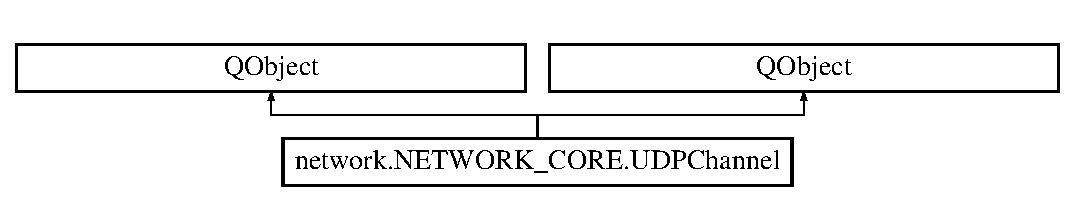
\includegraphics[height=2.000000cm]{classnetwork_1_1NETWORK__CORE_1_1UDPChannel}
\end{center}
\end{figure}
\subsection*{Public Member Functions}
\begin{DoxyCompactItemize}
\item 
def \hyperlink{classnetwork_1_1NETWORK__CORE_1_1UDPChannel_a628f06fad9f7da98bbc9b5b6630271ea}{\+\_\+\+\_\+init\+\_\+\+\_\+}
\item 
def \hyperlink{classnetwork_1_1NETWORK__CORE_1_1UDPChannel_ada99dd7f7ad27fc1db37062daf953e1c}{send}
\item 
def \hyperlink{classnetwork_1_1NETWORK__CORE_1_1UDPChannel_ada99dd7f7ad27fc1db37062daf953e1c}{send}
\item 
def \hyperlink{classnetwork_1_1NETWORK__CORE_1_1UDPChannel_a3b4c88da7b885083e8aa44aef436e8e6}{recv}
\item 
def \hyperlink{classnetwork_1_1NETWORK__CORE_1_1UDPChannel_a6edcb5683390f03f4b72e0525bc4e1f7}{receive\+Function}
\item 
def \hyperlink{classnetwork_1_1NETWORK__CORE_1_1UDPChannel_a713bd6e7b9bbe515669fe8e23981be8d}{start\+Recv}
\item 
def \hyperlink{classnetwork_1_1NETWORK__CORE_1_1UDPChannel_aa5a9c175e34181c0aa2b49ad2f9b10f6}{stop\+Recv}
\item 
def \hyperlink{classnetwork_1_1NETWORK__CORE_1_1UDPChannel_a628f06fad9f7da98bbc9b5b6630271ea}{\+\_\+\+\_\+init\+\_\+\+\_\+}
\item 
def \hyperlink{classnetwork_1_1NETWORK__CORE_1_1UDPChannel_ada99dd7f7ad27fc1db37062daf953e1c}{send}
\item 
def \hyperlink{classnetwork_1_1NETWORK__CORE_1_1UDPChannel_ada99dd7f7ad27fc1db37062daf953e1c}{send}
\item 
def \hyperlink{classnetwork_1_1NETWORK__CORE_1_1UDPChannel_a3b4c88da7b885083e8aa44aef436e8e6}{recv}
\item 
def \hyperlink{classnetwork_1_1NETWORK__CORE_1_1UDPChannel_a6edcb5683390f03f4b72e0525bc4e1f7}{receive\+Function}
\item 
def \hyperlink{classnetwork_1_1NETWORK__CORE_1_1UDPChannel_a713bd6e7b9bbe515669fe8e23981be8d}{start\+Recv}
\item 
def \hyperlink{classnetwork_1_1NETWORK__CORE_1_1UDPChannel_aa5a9c175e34181c0aa2b49ad2f9b10f6}{stop\+Recv}
\end{DoxyCompactItemize}
\subsection*{Public Attributes}
\begin{DoxyCompactItemize}
\item 
\hyperlink{classnetwork_1_1NETWORK__CORE_1_1UDPChannel_a109eaf924bea52d095c5ecf68eb105ca}{num}
\item 
\hyperlink{classnetwork_1_1NETWORK__CORE_1_1UDPChannel_afc8c05885afa164854d35e9ce5a5cca9}{ip}
\item 
\hyperlink{classnetwork_1_1NETWORK__CORE_1_1UDPChannel_a020849db64086f44fb76565a2fac454e}{port}
\item 
\hyperlink{classnetwork_1_1NETWORK__CORE_1_1UDPChannel_aea64337d89b2d361b8631e0c54316567}{sock}
\item 
\hyperlink{classnetwork_1_1NETWORK__CORE_1_1UDPChannel_a8cead572d015248b58dafbcb0e7f4043}{thread}
\end{DoxyCompactItemize}
\subsection*{Static Public Attributes}
\begin{DoxyCompactItemize}
\item 
tuple \hyperlink{classnetwork_1_1NETWORK__CORE_1_1UDPChannel_aafe450b69fd43efc0912db494a042b42}{recv\+Event} = Qt\+Core.\+pyqt\+Signal(int, str,tuple)
\begin{DoxyCompactList}\small\item\em signal for a received message. \end{DoxyCompactList}\end{DoxyCompactItemize}


\subsection{Constructor \& Destructor Documentation}
\hypertarget{classnetwork_1_1NETWORK__CORE_1_1UDPChannel_a628f06fad9f7da98bbc9b5b6630271ea}{}\index{network\+::\+N\+E\+T\+W\+O\+R\+K\+\_\+\+C\+O\+R\+E\+::\+U\+D\+P\+Channel@{network\+::\+N\+E\+T\+W\+O\+R\+K\+\_\+\+C\+O\+R\+E\+::\+U\+D\+P\+Channel}!\+\_\+\+\_\+init\+\_\+\+\_\+@{\+\_\+\+\_\+init\+\_\+\+\_\+}}
\index{\+\_\+\+\_\+init\+\_\+\+\_\+@{\+\_\+\+\_\+init\+\_\+\+\_\+}!network\+::\+N\+E\+T\+W\+O\+R\+K\+\_\+\+C\+O\+R\+E\+::\+U\+D\+P\+Channel@{network\+::\+N\+E\+T\+W\+O\+R\+K\+\_\+\+C\+O\+R\+E\+::\+U\+D\+P\+Channel}}
\subsubsection[{\+\_\+\+\_\+init\+\_\+\+\_\+}]{\setlength{\rightskip}{0pt plus 5cm}def network.\+N\+E\+T\+W\+O\+R\+K\+\_\+\+C\+O\+R\+E.\+U\+D\+P\+Channel.\+\_\+\+\_\+init\+\_\+\+\_\+ (
\begin{DoxyParamCaption}
\item[{}]{self, }
\item[{}]{num, }
\item[{}]{ip, }
\item[{}]{port, }
\item[{}]{timeout = {\ttfamily 1}}
\end{DoxyParamCaption}
)}\label{classnetwork_1_1NETWORK__CORE_1_1UDPChannel_a628f06fad9f7da98bbc9b5b6630271ea}
\hypertarget{classnetwork_1_1NETWORK__CORE_1_1UDPChannel_a628f06fad9f7da98bbc9b5b6630271ea}{}\index{network\+::\+N\+E\+T\+W\+O\+R\+K\+\_\+\+C\+O\+R\+E\+::\+U\+D\+P\+Channel@{network\+::\+N\+E\+T\+W\+O\+R\+K\+\_\+\+C\+O\+R\+E\+::\+U\+D\+P\+Channel}!\+\_\+\+\_\+init\+\_\+\+\_\+@{\+\_\+\+\_\+init\+\_\+\+\_\+}}
\index{\+\_\+\+\_\+init\+\_\+\+\_\+@{\+\_\+\+\_\+init\+\_\+\+\_\+}!network\+::\+N\+E\+T\+W\+O\+R\+K\+\_\+\+C\+O\+R\+E\+::\+U\+D\+P\+Channel@{network\+::\+N\+E\+T\+W\+O\+R\+K\+\_\+\+C\+O\+R\+E\+::\+U\+D\+P\+Channel}}
\subsubsection[{\+\_\+\+\_\+init\+\_\+\+\_\+}]{\setlength{\rightskip}{0pt plus 5cm}def network.\+N\+E\+T\+W\+O\+R\+K\+\_\+\+C\+O\+R\+E.\+U\+D\+P\+Channel.\+\_\+\+\_\+init\+\_\+\+\_\+ (
\begin{DoxyParamCaption}
\item[{}]{self, }
\item[{}]{num, }
\item[{}]{ip, }
\item[{}]{port, }
\item[{}]{timeout = {\ttfamily 1}}
\end{DoxyParamCaption}
)}\label{classnetwork_1_1NETWORK__CORE_1_1UDPChannel_a628f06fad9f7da98bbc9b5b6630271ea}


\subsection{Member Function Documentation}
\hypertarget{classnetwork_1_1NETWORK__CORE_1_1UDPChannel_a6edcb5683390f03f4b72e0525bc4e1f7}{}\index{network\+::\+N\+E\+T\+W\+O\+R\+K\+\_\+\+C\+O\+R\+E\+::\+U\+D\+P\+Channel@{network\+::\+N\+E\+T\+W\+O\+R\+K\+\_\+\+C\+O\+R\+E\+::\+U\+D\+P\+Channel}!receive\+Function@{receive\+Function}}
\index{receive\+Function@{receive\+Function}!network\+::\+N\+E\+T\+W\+O\+R\+K\+\_\+\+C\+O\+R\+E\+::\+U\+D\+P\+Channel@{network\+::\+N\+E\+T\+W\+O\+R\+K\+\_\+\+C\+O\+R\+E\+::\+U\+D\+P\+Channel}}
\subsubsection[{receive\+Function}]{\setlength{\rightskip}{0pt plus 5cm}def network.\+N\+E\+T\+W\+O\+R\+K\+\_\+\+C\+O\+R\+E.\+U\+D\+P\+Channel.\+receive\+Function (
\begin{DoxyParamCaption}
\item[{}]{self, }
\item[{}]{funct}
\end{DoxyParamCaption}
)}\label{classnetwork_1_1NETWORK__CORE_1_1UDPChannel_a6edcb5683390f03f4b72e0525bc4e1f7}
\hypertarget{classnetwork_1_1NETWORK__CORE_1_1UDPChannel_a6edcb5683390f03f4b72e0525bc4e1f7}{}\index{network\+::\+N\+E\+T\+W\+O\+R\+K\+\_\+\+C\+O\+R\+E\+::\+U\+D\+P\+Channel@{network\+::\+N\+E\+T\+W\+O\+R\+K\+\_\+\+C\+O\+R\+E\+::\+U\+D\+P\+Channel}!receive\+Function@{receive\+Function}}
\index{receive\+Function@{receive\+Function}!network\+::\+N\+E\+T\+W\+O\+R\+K\+\_\+\+C\+O\+R\+E\+::\+U\+D\+P\+Channel@{network\+::\+N\+E\+T\+W\+O\+R\+K\+\_\+\+C\+O\+R\+E\+::\+U\+D\+P\+Channel}}
\subsubsection[{receive\+Function}]{\setlength{\rightskip}{0pt plus 5cm}def network.\+N\+E\+T\+W\+O\+R\+K\+\_\+\+C\+O\+R\+E.\+U\+D\+P\+Channel.\+receive\+Function (
\begin{DoxyParamCaption}
\item[{}]{self, }
\item[{}]{funct}
\end{DoxyParamCaption}
)}\label{classnetwork_1_1NETWORK__CORE_1_1UDPChannel_a6edcb5683390f03f4b72e0525bc4e1f7}
\hypertarget{classnetwork_1_1NETWORK__CORE_1_1UDPChannel_a3b4c88da7b885083e8aa44aef436e8e6}{}\index{network\+::\+N\+E\+T\+W\+O\+R\+K\+\_\+\+C\+O\+R\+E\+::\+U\+D\+P\+Channel@{network\+::\+N\+E\+T\+W\+O\+R\+K\+\_\+\+C\+O\+R\+E\+::\+U\+D\+P\+Channel}!recv@{recv}}
\index{recv@{recv}!network\+::\+N\+E\+T\+W\+O\+R\+K\+\_\+\+C\+O\+R\+E\+::\+U\+D\+P\+Channel@{network\+::\+N\+E\+T\+W\+O\+R\+K\+\_\+\+C\+O\+R\+E\+::\+U\+D\+P\+Channel}}
\subsubsection[{recv}]{\setlength{\rightskip}{0pt plus 5cm}def network.\+N\+E\+T\+W\+O\+R\+K\+\_\+\+C\+O\+R\+E.\+U\+D\+P\+Channel.\+recv (
\begin{DoxyParamCaption}
\item[{}]{self, }
\item[{}]{num, }
\item[{}]{buf = {\ttfamily 1024}}
\end{DoxyParamCaption}
)}\label{classnetwork_1_1NETWORK__CORE_1_1UDPChannel_a3b4c88da7b885083e8aa44aef436e8e6}
\hypertarget{classnetwork_1_1NETWORK__CORE_1_1UDPChannel_a3b4c88da7b885083e8aa44aef436e8e6}{}\index{network\+::\+N\+E\+T\+W\+O\+R\+K\+\_\+\+C\+O\+R\+E\+::\+U\+D\+P\+Channel@{network\+::\+N\+E\+T\+W\+O\+R\+K\+\_\+\+C\+O\+R\+E\+::\+U\+D\+P\+Channel}!recv@{recv}}
\index{recv@{recv}!network\+::\+N\+E\+T\+W\+O\+R\+K\+\_\+\+C\+O\+R\+E\+::\+U\+D\+P\+Channel@{network\+::\+N\+E\+T\+W\+O\+R\+K\+\_\+\+C\+O\+R\+E\+::\+U\+D\+P\+Channel}}
\subsubsection[{recv}]{\setlength{\rightskip}{0pt plus 5cm}def network.\+N\+E\+T\+W\+O\+R\+K\+\_\+\+C\+O\+R\+E.\+U\+D\+P\+Channel.\+recv (
\begin{DoxyParamCaption}
\item[{}]{self, }
\item[{}]{num, }
\item[{}]{buf = {\ttfamily 1024}}
\end{DoxyParamCaption}
)}\label{classnetwork_1_1NETWORK__CORE_1_1UDPChannel_a3b4c88da7b885083e8aa44aef436e8e6}
\hypertarget{classnetwork_1_1NETWORK__CORE_1_1UDPChannel_ada99dd7f7ad27fc1db37062daf953e1c}{}\index{network\+::\+N\+E\+T\+W\+O\+R\+K\+\_\+\+C\+O\+R\+E\+::\+U\+D\+P\+Channel@{network\+::\+N\+E\+T\+W\+O\+R\+K\+\_\+\+C\+O\+R\+E\+::\+U\+D\+P\+Channel}!send@{send}}
\index{send@{send}!network\+::\+N\+E\+T\+W\+O\+R\+K\+\_\+\+C\+O\+R\+E\+::\+U\+D\+P\+Channel@{network\+::\+N\+E\+T\+W\+O\+R\+K\+\_\+\+C\+O\+R\+E\+::\+U\+D\+P\+Channel}}
\subsubsection[{send}]{\setlength{\rightskip}{0pt plus 5cm}def network.\+N\+E\+T\+W\+O\+R\+K\+\_\+\+C\+O\+R\+E.\+U\+D\+P\+Channel.\+send (
\begin{DoxyParamCaption}
\item[{}]{self, }
\item[{}]{msg}
\end{DoxyParamCaption}
)}\label{classnetwork_1_1NETWORK__CORE_1_1UDPChannel_ada99dd7f7ad27fc1db37062daf953e1c}
\hypertarget{classnetwork_1_1NETWORK__CORE_1_1UDPChannel_ada99dd7f7ad27fc1db37062daf953e1c}{}\index{network\+::\+N\+E\+T\+W\+O\+R\+K\+\_\+\+C\+O\+R\+E\+::\+U\+D\+P\+Channel@{network\+::\+N\+E\+T\+W\+O\+R\+K\+\_\+\+C\+O\+R\+E\+::\+U\+D\+P\+Channel}!send@{send}}
\index{send@{send}!network\+::\+N\+E\+T\+W\+O\+R\+K\+\_\+\+C\+O\+R\+E\+::\+U\+D\+P\+Channel@{network\+::\+N\+E\+T\+W\+O\+R\+K\+\_\+\+C\+O\+R\+E\+::\+U\+D\+P\+Channel}}
\subsubsection[{send}]{\setlength{\rightskip}{0pt plus 5cm}def network.\+N\+E\+T\+W\+O\+R\+K\+\_\+\+C\+O\+R\+E.\+U\+D\+P\+Channel.\+send (
\begin{DoxyParamCaption}
\item[{}]{self, }
\item[{}]{msg}
\end{DoxyParamCaption}
)}\label{classnetwork_1_1NETWORK__CORE_1_1UDPChannel_ada99dd7f7ad27fc1db37062daf953e1c}
\hypertarget{classnetwork_1_1NETWORK__CORE_1_1UDPChannel_ada99dd7f7ad27fc1db37062daf953e1c}{}\index{network\+::\+N\+E\+T\+W\+O\+R\+K\+\_\+\+C\+O\+R\+E\+::\+U\+D\+P\+Channel@{network\+::\+N\+E\+T\+W\+O\+R\+K\+\_\+\+C\+O\+R\+E\+::\+U\+D\+P\+Channel}!send@{send}}
\index{send@{send}!network\+::\+N\+E\+T\+W\+O\+R\+K\+\_\+\+C\+O\+R\+E\+::\+U\+D\+P\+Channel@{network\+::\+N\+E\+T\+W\+O\+R\+K\+\_\+\+C\+O\+R\+E\+::\+U\+D\+P\+Channel}}
\subsubsection[{send}]{\setlength{\rightskip}{0pt plus 5cm}def network.\+N\+E\+T\+W\+O\+R\+K\+\_\+\+C\+O\+R\+E.\+U\+D\+P\+Channel.\+send (
\begin{DoxyParamCaption}
\item[{}]{self, }
\item[{}]{msg, }
\item[{}]{ip, }
\item[{}]{port}
\end{DoxyParamCaption}
)}\label{classnetwork_1_1NETWORK__CORE_1_1UDPChannel_ada99dd7f7ad27fc1db37062daf953e1c}
\hypertarget{classnetwork_1_1NETWORK__CORE_1_1UDPChannel_ada99dd7f7ad27fc1db37062daf953e1c}{}\index{network\+::\+N\+E\+T\+W\+O\+R\+K\+\_\+\+C\+O\+R\+E\+::\+U\+D\+P\+Channel@{network\+::\+N\+E\+T\+W\+O\+R\+K\+\_\+\+C\+O\+R\+E\+::\+U\+D\+P\+Channel}!send@{send}}
\index{send@{send}!network\+::\+N\+E\+T\+W\+O\+R\+K\+\_\+\+C\+O\+R\+E\+::\+U\+D\+P\+Channel@{network\+::\+N\+E\+T\+W\+O\+R\+K\+\_\+\+C\+O\+R\+E\+::\+U\+D\+P\+Channel}}
\subsubsection[{send}]{\setlength{\rightskip}{0pt plus 5cm}def network.\+N\+E\+T\+W\+O\+R\+K\+\_\+\+C\+O\+R\+E.\+U\+D\+P\+Channel.\+send (
\begin{DoxyParamCaption}
\item[{}]{self, }
\item[{}]{msg, }
\item[{}]{ip, }
\item[{}]{port}
\end{DoxyParamCaption}
)}\label{classnetwork_1_1NETWORK__CORE_1_1UDPChannel_ada99dd7f7ad27fc1db37062daf953e1c}
\hypertarget{classnetwork_1_1NETWORK__CORE_1_1UDPChannel_a713bd6e7b9bbe515669fe8e23981be8d}{}\index{network\+::\+N\+E\+T\+W\+O\+R\+K\+\_\+\+C\+O\+R\+E\+::\+U\+D\+P\+Channel@{network\+::\+N\+E\+T\+W\+O\+R\+K\+\_\+\+C\+O\+R\+E\+::\+U\+D\+P\+Channel}!start\+Recv@{start\+Recv}}
\index{start\+Recv@{start\+Recv}!network\+::\+N\+E\+T\+W\+O\+R\+K\+\_\+\+C\+O\+R\+E\+::\+U\+D\+P\+Channel@{network\+::\+N\+E\+T\+W\+O\+R\+K\+\_\+\+C\+O\+R\+E\+::\+U\+D\+P\+Channel}}
\subsubsection[{start\+Recv}]{\setlength{\rightskip}{0pt plus 5cm}def network.\+N\+E\+T\+W\+O\+R\+K\+\_\+\+C\+O\+R\+E.\+U\+D\+P\+Channel.\+start\+Recv (
\begin{DoxyParamCaption}
\item[{}]{self}
\end{DoxyParamCaption}
)}\label{classnetwork_1_1NETWORK__CORE_1_1UDPChannel_a713bd6e7b9bbe515669fe8e23981be8d}
\hypertarget{classnetwork_1_1NETWORK__CORE_1_1UDPChannel_a713bd6e7b9bbe515669fe8e23981be8d}{}\index{network\+::\+N\+E\+T\+W\+O\+R\+K\+\_\+\+C\+O\+R\+E\+::\+U\+D\+P\+Channel@{network\+::\+N\+E\+T\+W\+O\+R\+K\+\_\+\+C\+O\+R\+E\+::\+U\+D\+P\+Channel}!start\+Recv@{start\+Recv}}
\index{start\+Recv@{start\+Recv}!network\+::\+N\+E\+T\+W\+O\+R\+K\+\_\+\+C\+O\+R\+E\+::\+U\+D\+P\+Channel@{network\+::\+N\+E\+T\+W\+O\+R\+K\+\_\+\+C\+O\+R\+E\+::\+U\+D\+P\+Channel}}
\subsubsection[{start\+Recv}]{\setlength{\rightskip}{0pt plus 5cm}def network.\+N\+E\+T\+W\+O\+R\+K\+\_\+\+C\+O\+R\+E.\+U\+D\+P\+Channel.\+start\+Recv (
\begin{DoxyParamCaption}
\item[{}]{self}
\end{DoxyParamCaption}
)}\label{classnetwork_1_1NETWORK__CORE_1_1UDPChannel_a713bd6e7b9bbe515669fe8e23981be8d}
\hypertarget{classnetwork_1_1NETWORK__CORE_1_1UDPChannel_aa5a9c175e34181c0aa2b49ad2f9b10f6}{}\index{network\+::\+N\+E\+T\+W\+O\+R\+K\+\_\+\+C\+O\+R\+E\+::\+U\+D\+P\+Channel@{network\+::\+N\+E\+T\+W\+O\+R\+K\+\_\+\+C\+O\+R\+E\+::\+U\+D\+P\+Channel}!stop\+Recv@{stop\+Recv}}
\index{stop\+Recv@{stop\+Recv}!network\+::\+N\+E\+T\+W\+O\+R\+K\+\_\+\+C\+O\+R\+E\+::\+U\+D\+P\+Channel@{network\+::\+N\+E\+T\+W\+O\+R\+K\+\_\+\+C\+O\+R\+E\+::\+U\+D\+P\+Channel}}
\subsubsection[{stop\+Recv}]{\setlength{\rightskip}{0pt plus 5cm}def network.\+N\+E\+T\+W\+O\+R\+K\+\_\+\+C\+O\+R\+E.\+U\+D\+P\+Channel.\+stop\+Recv (
\begin{DoxyParamCaption}
\item[{}]{self}
\end{DoxyParamCaption}
)}\label{classnetwork_1_1NETWORK__CORE_1_1UDPChannel_aa5a9c175e34181c0aa2b49ad2f9b10f6}
\hypertarget{classnetwork_1_1NETWORK__CORE_1_1UDPChannel_aa5a9c175e34181c0aa2b49ad2f9b10f6}{}\index{network\+::\+N\+E\+T\+W\+O\+R\+K\+\_\+\+C\+O\+R\+E\+::\+U\+D\+P\+Channel@{network\+::\+N\+E\+T\+W\+O\+R\+K\+\_\+\+C\+O\+R\+E\+::\+U\+D\+P\+Channel}!stop\+Recv@{stop\+Recv}}
\index{stop\+Recv@{stop\+Recv}!network\+::\+N\+E\+T\+W\+O\+R\+K\+\_\+\+C\+O\+R\+E\+::\+U\+D\+P\+Channel@{network\+::\+N\+E\+T\+W\+O\+R\+K\+\_\+\+C\+O\+R\+E\+::\+U\+D\+P\+Channel}}
\subsubsection[{stop\+Recv}]{\setlength{\rightskip}{0pt plus 5cm}def network.\+N\+E\+T\+W\+O\+R\+K\+\_\+\+C\+O\+R\+E.\+U\+D\+P\+Channel.\+stop\+Recv (
\begin{DoxyParamCaption}
\item[{}]{self}
\end{DoxyParamCaption}
)}\label{classnetwork_1_1NETWORK__CORE_1_1UDPChannel_aa5a9c175e34181c0aa2b49ad2f9b10f6}


\subsection{Member Data Documentation}
\hypertarget{classnetwork_1_1NETWORK__CORE_1_1UDPChannel_afc8c05885afa164854d35e9ce5a5cca9}{}\index{network\+::\+N\+E\+T\+W\+O\+R\+K\+\_\+\+C\+O\+R\+E\+::\+U\+D\+P\+Channel@{network\+::\+N\+E\+T\+W\+O\+R\+K\+\_\+\+C\+O\+R\+E\+::\+U\+D\+P\+Channel}!ip@{ip}}
\index{ip@{ip}!network\+::\+N\+E\+T\+W\+O\+R\+K\+\_\+\+C\+O\+R\+E\+::\+U\+D\+P\+Channel@{network\+::\+N\+E\+T\+W\+O\+R\+K\+\_\+\+C\+O\+R\+E\+::\+U\+D\+P\+Channel}}
\subsubsection[{ip}]{\setlength{\rightskip}{0pt plus 5cm}network.\+N\+E\+T\+W\+O\+R\+K\+\_\+\+C\+O\+R\+E.\+U\+D\+P\+Channel.\+ip}\label{classnetwork_1_1NETWORK__CORE_1_1UDPChannel_afc8c05885afa164854d35e9ce5a5cca9}
\hypertarget{classnetwork_1_1NETWORK__CORE_1_1UDPChannel_a109eaf924bea52d095c5ecf68eb105ca}{}\index{network\+::\+N\+E\+T\+W\+O\+R\+K\+\_\+\+C\+O\+R\+E\+::\+U\+D\+P\+Channel@{network\+::\+N\+E\+T\+W\+O\+R\+K\+\_\+\+C\+O\+R\+E\+::\+U\+D\+P\+Channel}!num@{num}}
\index{num@{num}!network\+::\+N\+E\+T\+W\+O\+R\+K\+\_\+\+C\+O\+R\+E\+::\+U\+D\+P\+Channel@{network\+::\+N\+E\+T\+W\+O\+R\+K\+\_\+\+C\+O\+R\+E\+::\+U\+D\+P\+Channel}}
\subsubsection[{num}]{\setlength{\rightskip}{0pt plus 5cm}network.\+N\+E\+T\+W\+O\+R\+K\+\_\+\+C\+O\+R\+E.\+U\+D\+P\+Channel.\+num}\label{classnetwork_1_1NETWORK__CORE_1_1UDPChannel_a109eaf924bea52d095c5ecf68eb105ca}
\hypertarget{classnetwork_1_1NETWORK__CORE_1_1UDPChannel_a020849db64086f44fb76565a2fac454e}{}\index{network\+::\+N\+E\+T\+W\+O\+R\+K\+\_\+\+C\+O\+R\+E\+::\+U\+D\+P\+Channel@{network\+::\+N\+E\+T\+W\+O\+R\+K\+\_\+\+C\+O\+R\+E\+::\+U\+D\+P\+Channel}!port@{port}}
\index{port@{port}!network\+::\+N\+E\+T\+W\+O\+R\+K\+\_\+\+C\+O\+R\+E\+::\+U\+D\+P\+Channel@{network\+::\+N\+E\+T\+W\+O\+R\+K\+\_\+\+C\+O\+R\+E\+::\+U\+D\+P\+Channel}}
\subsubsection[{port}]{\setlength{\rightskip}{0pt plus 5cm}network.\+N\+E\+T\+W\+O\+R\+K\+\_\+\+C\+O\+R\+E.\+U\+D\+P\+Channel.\+port}\label{classnetwork_1_1NETWORK__CORE_1_1UDPChannel_a020849db64086f44fb76565a2fac454e}
\hypertarget{classnetwork_1_1NETWORK__CORE_1_1UDPChannel_aafe450b69fd43efc0912db494a042b42}{}\index{network\+::\+N\+E\+T\+W\+O\+R\+K\+\_\+\+C\+O\+R\+E\+::\+U\+D\+P\+Channel@{network\+::\+N\+E\+T\+W\+O\+R\+K\+\_\+\+C\+O\+R\+E\+::\+U\+D\+P\+Channel}!recv\+Event@{recv\+Event}}
\index{recv\+Event@{recv\+Event}!network\+::\+N\+E\+T\+W\+O\+R\+K\+\_\+\+C\+O\+R\+E\+::\+U\+D\+P\+Channel@{network\+::\+N\+E\+T\+W\+O\+R\+K\+\_\+\+C\+O\+R\+E\+::\+U\+D\+P\+Channel}}
\subsubsection[{recv\+Event}]{\setlength{\rightskip}{0pt plus 5cm}tuple network.\+N\+E\+T\+W\+O\+R\+K\+\_\+\+C\+O\+R\+E.\+U\+D\+P\+Channel.\+recv\+Event = Qt\+Core.\+pyqt\+Signal(int, str,tuple)\hspace{0.3cm}{\ttfamily [static]}}\label{classnetwork_1_1NETWORK__CORE_1_1UDPChannel_aafe450b69fd43efc0912db494a042b42}


signal for a received message. 

\hypertarget{classnetwork_1_1NETWORK__CORE_1_1UDPChannel_aea64337d89b2d361b8631e0c54316567}{}\index{network\+::\+N\+E\+T\+W\+O\+R\+K\+\_\+\+C\+O\+R\+E\+::\+U\+D\+P\+Channel@{network\+::\+N\+E\+T\+W\+O\+R\+K\+\_\+\+C\+O\+R\+E\+::\+U\+D\+P\+Channel}!sock@{sock}}
\index{sock@{sock}!network\+::\+N\+E\+T\+W\+O\+R\+K\+\_\+\+C\+O\+R\+E\+::\+U\+D\+P\+Channel@{network\+::\+N\+E\+T\+W\+O\+R\+K\+\_\+\+C\+O\+R\+E\+::\+U\+D\+P\+Channel}}
\subsubsection[{sock}]{\setlength{\rightskip}{0pt plus 5cm}network.\+N\+E\+T\+W\+O\+R\+K\+\_\+\+C\+O\+R\+E.\+U\+D\+P\+Channel.\+sock}\label{classnetwork_1_1NETWORK__CORE_1_1UDPChannel_aea64337d89b2d361b8631e0c54316567}
\hypertarget{classnetwork_1_1NETWORK__CORE_1_1UDPChannel_a8cead572d015248b58dafbcb0e7f4043}{}\index{network\+::\+N\+E\+T\+W\+O\+R\+K\+\_\+\+C\+O\+R\+E\+::\+U\+D\+P\+Channel@{network\+::\+N\+E\+T\+W\+O\+R\+K\+\_\+\+C\+O\+R\+E\+::\+U\+D\+P\+Channel}!thread@{thread}}
\index{thread@{thread}!network\+::\+N\+E\+T\+W\+O\+R\+K\+\_\+\+C\+O\+R\+E\+::\+U\+D\+P\+Channel@{network\+::\+N\+E\+T\+W\+O\+R\+K\+\_\+\+C\+O\+R\+E\+::\+U\+D\+P\+Channel}}
\subsubsection[{thread}]{\setlength{\rightskip}{0pt plus 5cm}network.\+N\+E\+T\+W\+O\+R\+K\+\_\+\+C\+O\+R\+E.\+U\+D\+P\+Channel.\+thread}\label{classnetwork_1_1NETWORK__CORE_1_1UDPChannel_a8cead572d015248b58dafbcb0e7f4043}


The documentation for this class was generated from the following file\+:\begin{DoxyCompactItemize}
\item 
build/lib.\+linux-\/x86\+\_\+64-\/2.\+7/network/\hyperlink{build_2lib_8linux-x86__64-2_87_2network_2NETWORK__CORE_8py}{N\+E\+T\+W\+O\+R\+K\+\_\+\+C\+O\+R\+E.\+py}\end{DoxyCompactItemize}

\chapter{File Documentation}
\hypertarget{build_2lib_8linux-x86__64-2_87_2controller_2____init_____8py}{}\section{build/lib.linux-\/x86\+\_\+64-\/2.7/controller/\+\_\+\+\_\+init\+\_\+\+\_\+.py File Reference}
\label{build_2lib_8linux-x86__64-2_87_2controller_2____init_____8py}\index{build/lib.\+linux-\/x86\+\_\+64-\/2.\+7/controller/\+\_\+\+\_\+init\+\_\+\+\_\+.\+py@{build/lib.\+linux-\/x86\+\_\+64-\/2.\+7/controller/\+\_\+\+\_\+init\+\_\+\+\_\+.\+py}}
\subsection*{Namespaces}
\begin{DoxyCompactItemize}
\item 
 \hyperlink{namespacecontroller}{controller}
\end{DoxyCompactItemize}

\hypertarget{build_2lib_8linux-x86__64-2_87_2driver_2____init_____8py}{}\section{build/lib.linux-\/x86\+\_\+64-\/2.7/driver/\+\_\+\+\_\+init\+\_\+\+\_\+.py File Reference}
\label{build_2lib_8linux-x86__64-2_87_2driver_2____init_____8py}\index{build/lib.\+linux-\/x86\+\_\+64-\/2.\+7/driver/\+\_\+\+\_\+init\+\_\+\+\_\+.\+py@{build/lib.\+linux-\/x86\+\_\+64-\/2.\+7/driver/\+\_\+\+\_\+init\+\_\+\+\_\+.\+py}}
\subsection*{Namespaces}
\begin{DoxyCompactItemize}
\item 
 \hyperlink{namespacedriver}{driver}
\end{DoxyCompactItemize}

\hypertarget{build_2lib_8linux-x86__64-2_87_2frost_2____init_____8py}{}\section{build/lib.linux-\/x86\+\_\+64-\/2.7/frost/\+\_\+\+\_\+init\+\_\+\+\_\+.py File Reference}
\label{build_2lib_8linux-x86__64-2_87_2frost_2____init_____8py}\index{build/lib.\+linux-\/x86\+\_\+64-\/2.\+7/frost/\+\_\+\+\_\+init\+\_\+\+\_\+.\+py@{build/lib.\+linux-\/x86\+\_\+64-\/2.\+7/frost/\+\_\+\+\_\+init\+\_\+\+\_\+.\+py}}
\subsection*{Namespaces}
\begin{DoxyCompactItemize}
\item 
 \hyperlink{namespacefrost}{frost}
\end{DoxyCompactItemize}

\hypertarget{build_2lib_8linux-x86__64-2_87_2interface_2____init_____8py}{}\section{build/lib.linux-\/x86\+\_\+64-\/2.7/interface/\+\_\+\+\_\+init\+\_\+\+\_\+.py File Reference}
\label{build_2lib_8linux-x86__64-2_87_2interface_2____init_____8py}\index{build/lib.\+linux-\/x86\+\_\+64-\/2.\+7/interface/\+\_\+\+\_\+init\+\_\+\+\_\+.\+py@{build/lib.\+linux-\/x86\+\_\+64-\/2.\+7/interface/\+\_\+\+\_\+init\+\_\+\+\_\+.\+py}}
\subsection*{Namespaces}
\begin{DoxyCompactItemize}
\item 
 \hyperlink{namespaceinterface}{interface}
\end{DoxyCompactItemize}

\hypertarget{build_2lib_8linux-x86__64-2_87_2model_2____init_____8py}{}\section{build/lib.linux-\/x86\+\_\+64-\/2.7/model/\+\_\+\+\_\+init\+\_\+\+\_\+.py File Reference}
\label{build_2lib_8linux-x86__64-2_87_2model_2____init_____8py}\index{build/lib.\+linux-\/x86\+\_\+64-\/2.\+7/model/\+\_\+\+\_\+init\+\_\+\+\_\+.\+py@{build/lib.\+linux-\/x86\+\_\+64-\/2.\+7/model/\+\_\+\+\_\+init\+\_\+\+\_\+.\+py}}
\subsection*{Namespaces}
\begin{DoxyCompactItemize}
\item 
 \hyperlink{namespacemodel}{model}
\end{DoxyCompactItemize}

\hypertarget{build_2lib_8linux-x86__64-2_87_2network_2____init_____8py}{}\section{build/lib.linux-\/x86\+\_\+64-\/2.7/network/\+\_\+\+\_\+init\+\_\+\+\_\+.py File Reference}
\label{build_2lib_8linux-x86__64-2_87_2network_2____init_____8py}\index{build/lib.\+linux-\/x86\+\_\+64-\/2.\+7/network/\+\_\+\+\_\+init\+\_\+\+\_\+.\+py@{build/lib.\+linux-\/x86\+\_\+64-\/2.\+7/network/\+\_\+\+\_\+init\+\_\+\+\_\+.\+py}}
\subsection*{Namespaces}
\begin{DoxyCompactItemize}
\item 
 \hyperlink{namespacenetwork}{network}
\end{DoxyCompactItemize}

\hypertarget{controller_2____init_____8py}{}\section{controller/\+\_\+\+\_\+init\+\_\+\+\_\+.py File Reference}
\label{controller_2____init_____8py}\index{controller/\+\_\+\+\_\+init\+\_\+\+\_\+.\+py@{controller/\+\_\+\+\_\+init\+\_\+\+\_\+.\+py}}
\subsection*{Namespaces}
\begin{DoxyCompactItemize}
\item 
 \hyperlink{namespacecontroller}{controller}
\end{DoxyCompactItemize}

\hypertarget{driver_2____init_____8py}{}\section{driver/\+\_\+\+\_\+init\+\_\+\+\_\+.py File Reference}
\label{driver_2____init_____8py}\index{driver/\+\_\+\+\_\+init\+\_\+\+\_\+.\+py@{driver/\+\_\+\+\_\+init\+\_\+\+\_\+.\+py}}
\subsection*{Namespaces}
\begin{DoxyCompactItemize}
\item 
 \hyperlink{namespacedriver}{driver}
\end{DoxyCompactItemize}

\hypertarget{frost_2____init_____8py}{}\section{frost/\+\_\+\+\_\+init\+\_\+\+\_\+.py File Reference}
\label{frost_2____init_____8py}\index{frost/\+\_\+\+\_\+init\+\_\+\+\_\+.\+py@{frost/\+\_\+\+\_\+init\+\_\+\+\_\+.\+py}}
\subsection*{Namespaces}
\begin{DoxyCompactItemize}
\item 
 \hyperlink{namespacefrost}{frost}
\end{DoxyCompactItemize}

\hypertarget{interface_2____init_____8py}{}\section{interface/\+\_\+\+\_\+init\+\_\+\+\_\+.py File Reference}
\label{interface_2____init_____8py}\index{interface/\+\_\+\+\_\+init\+\_\+\+\_\+.\+py@{interface/\+\_\+\+\_\+init\+\_\+\+\_\+.\+py}}
\subsection*{Namespaces}
\begin{DoxyCompactItemize}
\item 
 \hyperlink{namespaceinterface}{interface}
\end{DoxyCompactItemize}

\hypertarget{model_2____init_____8py}{}\section{model/\+\_\+\+\_\+init\+\_\+\+\_\+.py File Reference}
\label{model_2____init_____8py}\index{model/\+\_\+\+\_\+init\+\_\+\+\_\+.\+py@{model/\+\_\+\+\_\+init\+\_\+\+\_\+.\+py}}
\subsection*{Namespaces}
\begin{DoxyCompactItemize}
\item 
 \hyperlink{namespacemodel}{model}
\end{DoxyCompactItemize}

\hypertarget{network_2____init_____8py}{}\section{network/\+\_\+\+\_\+init\+\_\+\+\_\+.py File Reference}
\label{network_2____init_____8py}\index{network/\+\_\+\+\_\+init\+\_\+\+\_\+.\+py@{network/\+\_\+\+\_\+init\+\_\+\+\_\+.\+py}}
\subsection*{Namespaces}
\begin{DoxyCompactItemize}
\item 
 \hyperlink{namespacenetwork}{network}
\end{DoxyCompactItemize}

\hypertarget{build_2lib_8linux-x86__64-2_87_2controller_2baseController_8py}{}\section{build/lib.linux-\/x86\+\_\+64-\/2.7/controller/base\+Controller.py File Reference}
\label{build_2lib_8linux-x86__64-2_87_2controller_2baseController_8py}\index{build/lib.\+linux-\/x86\+\_\+64-\/2.\+7/controller/base\+Controller.\+py@{build/lib.\+linux-\/x86\+\_\+64-\/2.\+7/controller/base\+Controller.\+py}}
\subsection*{Namespaces}
\begin{DoxyCompactItemize}
\item 
 \hyperlink{namespacecontroller_1_1baseController}{controller.\+base\+Controller}
\end{DoxyCompactItemize}

\hypertarget{controller_2baseController_8py}{}\section{controller/base\+Controller.py File Reference}
\label{controller_2baseController_8py}\index{controller/base\+Controller.\+py@{controller/base\+Controller.\+py}}
\subsection*{Namespaces}
\begin{DoxyCompactItemize}
\item 
 \hyperlink{namespacecontroller_1_1baseController}{controller.\+base\+Controller}
\end{DoxyCompactItemize}

\hypertarget{build_2lib_8linux-x86__64-2_87_2controller_2controller_8py}{}\section{build/lib.linux-\/x86\+\_\+64-\/2.7/controller/controller.py File Reference}
\label{build_2lib_8linux-x86__64-2_87_2controller_2controller_8py}\index{build/lib.\+linux-\/x86\+\_\+64-\/2.\+7/controller/controller.\+py@{build/lib.\+linux-\/x86\+\_\+64-\/2.\+7/controller/controller.\+py}}
\subsection*{Classes}
\begin{DoxyCompactItemize}
\item 
class \hyperlink{classcontroller_1_1controller_1_1Controller}{controller.\+controller.\+Controller}
\end{DoxyCompactItemize}
\subsection*{Namespaces}
\begin{DoxyCompactItemize}
\item 
 \hyperlink{namespacecontroller_1_1controller}{controller.\+controller}
\end{DoxyCompactItemize}

\hypertarget{controller_2controller_8py}{}\section{controller/controller.py File Reference}
\label{controller_2controller_8py}\index{controller/controller.\+py@{controller/controller.\+py}}
\subsection*{Classes}
\begin{DoxyCompactItemize}
\item 
class \hyperlink{classcontroller_1_1controller_1_1Controller}{controller.\+controller.\+Controller}
\end{DoxyCompactItemize}
\subsection*{Namespaces}
\begin{DoxyCompactItemize}
\item 
 \hyperlink{namespacecontroller_1_1controller}{controller.\+controller}
\end{DoxyCompactItemize}

\hypertarget{build_2lib_8linux-x86__64-2_87_2driver_2DRIVER__CORE_8py}{}\section{build/lib.linux-\/x86\+\_\+64-\/2.7/driver/\+D\+R\+I\+V\+E\+R\+\_\+\+C\+O\+R\+E.py File Reference}
\label{build_2lib_8linux-x86__64-2_87_2driver_2DRIVER__CORE_8py}\index{build/lib.\+linux-\/x86\+\_\+64-\/2.\+7/driver/\+D\+R\+I\+V\+E\+R\+\_\+\+C\+O\+R\+E.\+py@{build/lib.\+linux-\/x86\+\_\+64-\/2.\+7/driver/\+D\+R\+I\+V\+E\+R\+\_\+\+C\+O\+R\+E.\+py}}
\subsection*{Classes}
\begin{DoxyCompactItemize}
\item 
class \hyperlink{classdriver_1_1DRIVER__CORE_1_1PCA9865}{driver.\+D\+R\+I\+V\+E\+R\+\_\+\+C\+O\+R\+E.\+P\+C\+A9865}
\item 
class \hyperlink{classdriver_1_1DRIVER__CORE_1_1Adafruit__LSM303}{driver.\+D\+R\+I\+V\+E\+R\+\_\+\+C\+O\+R\+E.\+Adafruit\+\_\+\+L\+S\+M303}
\item 
class \hyperlink{classdriver_1_1DRIVER__CORE_1_1LCD}{driver.\+D\+R\+I\+V\+E\+R\+\_\+\+C\+O\+R\+E.\+L\+C\+D}
\end{DoxyCompactItemize}
\subsection*{Namespaces}
\begin{DoxyCompactItemize}
\item 
 \hyperlink{namespacedriver_1_1DRIVER__CORE}{driver.\+D\+R\+I\+V\+E\+R\+\_\+\+C\+O\+R\+E}
\item 
 \hyperlink{namespacedocstring}{docstring}
\begin{DoxyCompactList}\small\item\em Complete Driver Collection of supported devices by F\+R\+O\+S\+T O\+S. \end{DoxyCompactList}\end{DoxyCompactItemize}

\hypertarget{driver_2DRIVER__CORE_8py}{}\section{driver/\+D\+R\+I\+V\+E\+R\+\_\+\+C\+O\+R\+E.py File Reference}
\label{driver_2DRIVER__CORE_8py}\index{driver/\+D\+R\+I\+V\+E\+R\+\_\+\+C\+O\+R\+E.\+py@{driver/\+D\+R\+I\+V\+E\+R\+\_\+\+C\+O\+R\+E.\+py}}
\subsection*{Classes}
\begin{DoxyCompactItemize}
\item 
class \hyperlink{classdriver_1_1DRIVER__CORE_1_1PCA9865}{driver.\+D\+R\+I\+V\+E\+R\+\_\+\+C\+O\+R\+E.\+P\+C\+A9865}
\item 
class \hyperlink{classdriver_1_1DRIVER__CORE_1_1Adafruit__LSM303}{driver.\+D\+R\+I\+V\+E\+R\+\_\+\+C\+O\+R\+E.\+Adafruit\+\_\+\+L\+S\+M303}
\item 
class \hyperlink{classdriver_1_1DRIVER__CORE_1_1LCD}{driver.\+D\+R\+I\+V\+E\+R\+\_\+\+C\+O\+R\+E.\+L\+C\+D}
\end{DoxyCompactItemize}
\subsection*{Namespaces}
\begin{DoxyCompactItemize}
\item 
 \hyperlink{namespacedriver_1_1DRIVER__CORE}{driver.\+D\+R\+I\+V\+E\+R\+\_\+\+C\+O\+R\+E}
\item 
 \hyperlink{namespacedocstring}{docstring}
\begin{DoxyCompactList}\small\item\em Complete Driver Collection of supported devices by F\+R\+O\+S\+T O\+S. \end{DoxyCompactList}\end{DoxyCompactItemize}

\hypertarget{build_2lib_8linux-x86__64-2_87_2driver_2i2c__lib_8py}{}\section{build/lib.linux-\/x86\+\_\+64-\/2.7/driver/i2c\+\_\+lib.py File Reference}
\label{build_2lib_8linux-x86__64-2_87_2driver_2i2c__lib_8py}\index{build/lib.\+linux-\/x86\+\_\+64-\/2.\+7/driver/i2c\+\_\+lib.\+py@{build/lib.\+linux-\/x86\+\_\+64-\/2.\+7/driver/i2c\+\_\+lib.\+py}}
\subsection*{Classes}
\begin{DoxyCompactItemize}
\item 
class \hyperlink{classdriver_1_1i2c__lib_1_1i2c__device}{driver.\+i2c\+\_\+lib.\+i2c\+\_\+device}
\end{DoxyCompactItemize}
\subsection*{Namespaces}
\begin{DoxyCompactItemize}
\item 
 \hyperlink{namespacedriver_1_1i2c__lib}{driver.\+i2c\+\_\+lib}
\end{DoxyCompactItemize}

\hypertarget{driver_2i2c__lib_8py}{}\section{driver/i2c\+\_\+lib.py File Reference}
\label{driver_2i2c__lib_8py}\index{driver/i2c\+\_\+lib.\+py@{driver/i2c\+\_\+lib.\+py}}
\subsection*{Classes}
\begin{DoxyCompactItemize}
\item 
class \hyperlink{classdriver_1_1i2c__lib_1_1i2c__device}{driver.\+i2c\+\_\+lib.\+i2c\+\_\+device}
\end{DoxyCompactItemize}
\subsection*{Namespaces}
\begin{DoxyCompactItemize}
\item 
 \hyperlink{namespacedriver_1_1i2c__lib}{driver.\+i2c\+\_\+lib}
\end{DoxyCompactItemize}

\hypertarget{build_2lib_8linux-x86__64-2_87_2driver_2LOGITECH__GAMEPAD__DRIVER_8py}{}\section{build/lib.linux-\/x86\+\_\+64-\/2.7/driver/\+L\+O\+G\+I\+T\+E\+C\+H\+\_\+\+G\+A\+M\+E\+P\+A\+D\+\_\+\+D\+R\+I\+V\+E\+R.py File Reference}
\label{build_2lib_8linux-x86__64-2_87_2driver_2LOGITECH__GAMEPAD__DRIVER_8py}\index{build/lib.\+linux-\/x86\+\_\+64-\/2.\+7/driver/\+L\+O\+G\+I\+T\+E\+C\+H\+\_\+\+G\+A\+M\+E\+P\+A\+D\+\_\+\+D\+R\+I\+V\+E\+R.\+py@{build/lib.\+linux-\/x86\+\_\+64-\/2.\+7/driver/\+L\+O\+G\+I\+T\+E\+C\+H\+\_\+\+G\+A\+M\+E\+P\+A\+D\+\_\+\+D\+R\+I\+V\+E\+R.\+py}}
\subsection*{Classes}
\begin{DoxyCompactItemize}
\item 
class \hyperlink{classdriver_1_1LOGITECH__GAMEPAD__DRIVER_1_1LogitechGamepadDriver}{driver.\+L\+O\+G\+I\+T\+E\+C\+H\+\_\+\+G\+A\+M\+E\+P\+A\+D\+\_\+\+D\+R\+I\+V\+E\+R.\+Logitech\+Gamepad\+Driver}
\item 
class \hyperlink{classdriver_1_1LOGITECH__GAMEPAD__DRIVER_1_1LogitechGamepadDriver_1_1GamepadThread}{driver.\+L\+O\+G\+I\+T\+E\+C\+H\+\_\+\+G\+A\+M\+E\+P\+A\+D\+\_\+\+D\+R\+I\+V\+E\+R.\+Logitech\+Gamepad\+Driver.\+Gamepad\+Thread}
\end{DoxyCompactItemize}
\subsection*{Namespaces}
\begin{DoxyCompactItemize}
\item 
 \hyperlink{namespacedriver_1_1LOGITECH__GAMEPAD__DRIVER}{driver.\+L\+O\+G\+I\+T\+E\+C\+H\+\_\+\+G\+A\+M\+E\+P\+A\+D\+\_\+\+D\+R\+I\+V\+E\+R}
\end{DoxyCompactItemize}
\subsection*{Functions}
\begin{DoxyCompactItemize}
\item 
def \hyperlink{namespacedriver_1_1LOGITECH__GAMEPAD__DRIVER_aaa658f6556352e0d77c8437b019f41f9}{driver.\+L\+O\+G\+I\+T\+E\+C\+H\+\_\+\+G\+A\+M\+E\+P\+A\+D\+\_\+\+D\+R\+I\+V\+E\+R.\+main}
\end{DoxyCompactItemize}

\hypertarget{driver_2LOGITECH__GAMEPAD__DRIVER_8py}{}\section{driver/\+L\+O\+G\+I\+T\+E\+C\+H\+\_\+\+G\+A\+M\+E\+P\+A\+D\+\_\+\+D\+R\+I\+V\+E\+R.py File Reference}
\label{driver_2LOGITECH__GAMEPAD__DRIVER_8py}\index{driver/\+L\+O\+G\+I\+T\+E\+C\+H\+\_\+\+G\+A\+M\+E\+P\+A\+D\+\_\+\+D\+R\+I\+V\+E\+R.\+py@{driver/\+L\+O\+G\+I\+T\+E\+C\+H\+\_\+\+G\+A\+M\+E\+P\+A\+D\+\_\+\+D\+R\+I\+V\+E\+R.\+py}}
\subsection*{Classes}
\begin{DoxyCompactItemize}
\item 
class \hyperlink{classdriver_1_1LOGITECH__GAMEPAD__DRIVER_1_1LogitechGamepadDriver}{driver.\+L\+O\+G\+I\+T\+E\+C\+H\+\_\+\+G\+A\+M\+E\+P\+A\+D\+\_\+\+D\+R\+I\+V\+E\+R.\+Logitech\+Gamepad\+Driver}
\item 
class \hyperlink{classdriver_1_1LOGITECH__GAMEPAD__DRIVER_1_1LogitechGamepadDriver_1_1GamepadThread}{driver.\+L\+O\+G\+I\+T\+E\+C\+H\+\_\+\+G\+A\+M\+E\+P\+A\+D\+\_\+\+D\+R\+I\+V\+E\+R.\+Logitech\+Gamepad\+Driver.\+Gamepad\+Thread}
\end{DoxyCompactItemize}
\subsection*{Namespaces}
\begin{DoxyCompactItemize}
\item 
 \hyperlink{namespacedriver_1_1LOGITECH__GAMEPAD__DRIVER}{driver.\+L\+O\+G\+I\+T\+E\+C\+H\+\_\+\+G\+A\+M\+E\+P\+A\+D\+\_\+\+D\+R\+I\+V\+E\+R}
\end{DoxyCompactItemize}
\subsection*{Functions}
\begin{DoxyCompactItemize}
\item 
def \hyperlink{namespacedriver_1_1LOGITECH__GAMEPAD__DRIVER_aaa658f6556352e0d77c8437b019f41f9}{driver.\+L\+O\+G\+I\+T\+E\+C\+H\+\_\+\+G\+A\+M\+E\+P\+A\+D\+\_\+\+D\+R\+I\+V\+E\+R.\+main}
\end{DoxyCompactItemize}

\hypertarget{build_2lib_8linux-x86__64-2_87_2interface_2INTERFACE__CORE_8py}{}\section{build/lib.linux-\/x86\+\_\+64-\/2.7/interface/\+I\+N\+T\+E\+R\+F\+A\+C\+E\+\_\+\+C\+O\+R\+E.py File Reference}
\label{build_2lib_8linux-x86__64-2_87_2interface_2INTERFACE__CORE_8py}\index{build/lib.\+linux-\/x86\+\_\+64-\/2.\+7/interface/\+I\+N\+T\+E\+R\+F\+A\+C\+E\+\_\+\+C\+O\+R\+E.\+py@{build/lib.\+linux-\/x86\+\_\+64-\/2.\+7/interface/\+I\+N\+T\+E\+R\+F\+A\+C\+E\+\_\+\+C\+O\+R\+E.\+py}}
\subsection*{Classes}
\begin{DoxyCompactItemize}
\item 
class \hyperlink{classinterface_1_1INTERFACE__CORE_1_1interface}{interface.\+I\+N\+T\+E\+R\+F\+A\+C\+E\+\_\+\+C\+O\+R\+E.\+interface}
\end{DoxyCompactItemize}
\subsection*{Namespaces}
\begin{DoxyCompactItemize}
\item 
 \hyperlink{namespaceinterface_1_1INTERFACE__CORE}{interface.\+I\+N\+T\+E\+R\+F\+A\+C\+E\+\_\+\+C\+O\+R\+E}
\end{DoxyCompactItemize}

\hypertarget{interface_2INTERFACE__CORE_8py}{}\section{interface/\+I\+N\+T\+E\+R\+F\+A\+C\+E\+\_\+\+C\+O\+R\+E.py File Reference}
\label{interface_2INTERFACE__CORE_8py}\index{interface/\+I\+N\+T\+E\+R\+F\+A\+C\+E\+\_\+\+C\+O\+R\+E.\+py@{interface/\+I\+N\+T\+E\+R\+F\+A\+C\+E\+\_\+\+C\+O\+R\+E.\+py}}
\subsection*{Classes}
\begin{DoxyCompactItemize}
\item 
class \hyperlink{classinterface_1_1INTERFACE__CORE_1_1interface}{interface.\+I\+N\+T\+E\+R\+F\+A\+C\+E\+\_\+\+C\+O\+R\+E.\+interface}
\end{DoxyCompactItemize}
\subsection*{Namespaces}
\begin{DoxyCompactItemize}
\item 
 \hyperlink{namespaceinterface_1_1INTERFACE__CORE}{interface.\+I\+N\+T\+E\+R\+F\+A\+C\+E\+\_\+\+C\+O\+R\+E}
\end{DoxyCompactItemize}

\hypertarget{build_2lib_8linux-x86__64-2_87_2interface_2LOGITECH__GAMEPAD__INTERFACE_8py}{}\section{build/lib.linux-\/x86\+\_\+64-\/2.7/interface/\+L\+O\+G\+I\+T\+E\+C\+H\+\_\+\+G\+A\+M\+E\+P\+A\+D\+\_\+\+I\+N\+T\+E\+R\+F\+A\+C\+E.py File Reference}
\label{build_2lib_8linux-x86__64-2_87_2interface_2LOGITECH__GAMEPAD__INTERFACE_8py}\index{build/lib.\+linux-\/x86\+\_\+64-\/2.\+7/interface/\+L\+O\+G\+I\+T\+E\+C\+H\+\_\+\+G\+A\+M\+E\+P\+A\+D\+\_\+\+I\+N\+T\+E\+R\+F\+A\+C\+E.\+py@{build/lib.\+linux-\/x86\+\_\+64-\/2.\+7/interface/\+L\+O\+G\+I\+T\+E\+C\+H\+\_\+\+G\+A\+M\+E\+P\+A\+D\+\_\+\+I\+N\+T\+E\+R\+F\+A\+C\+E.\+py}}
\subsection*{Classes}
\begin{DoxyCompactItemize}
\item 
class \hyperlink{classinterface_1_1LOGITECH__GAMEPAD__INTERFACE_1_1LogitechGamepadInterface}{interface.\+L\+O\+G\+I\+T\+E\+C\+H\+\_\+\+G\+A\+M\+E\+P\+A\+D\+\_\+\+I\+N\+T\+E\+R\+F\+A\+C\+E.\+Logitech\+Gamepad\+Interface}
\end{DoxyCompactItemize}
\subsection*{Namespaces}
\begin{DoxyCompactItemize}
\item 
 \hyperlink{namespaceinterface_1_1LOGITECH__GAMEPAD__INTERFACE}{interface.\+L\+O\+G\+I\+T\+E\+C\+H\+\_\+\+G\+A\+M\+E\+P\+A\+D\+\_\+\+I\+N\+T\+E\+R\+F\+A\+C\+E}
\end{DoxyCompactItemize}

\hypertarget{interface_2LOGITECH__GAMEPAD__INTERFACE_8py}{}\section{interface/\+L\+O\+G\+I\+T\+E\+C\+H\+\_\+\+G\+A\+M\+E\+P\+A\+D\+\_\+\+I\+N\+T\+E\+R\+F\+A\+C\+E.py File Reference}
\label{interface_2LOGITECH__GAMEPAD__INTERFACE_8py}\index{interface/\+L\+O\+G\+I\+T\+E\+C\+H\+\_\+\+G\+A\+M\+E\+P\+A\+D\+\_\+\+I\+N\+T\+E\+R\+F\+A\+C\+E.\+py@{interface/\+L\+O\+G\+I\+T\+E\+C\+H\+\_\+\+G\+A\+M\+E\+P\+A\+D\+\_\+\+I\+N\+T\+E\+R\+F\+A\+C\+E.\+py}}
\subsection*{Classes}
\begin{DoxyCompactItemize}
\item 
class \hyperlink{classinterface_1_1LOGITECH__GAMEPAD__INTERFACE_1_1LogitechGamepadInterface}{interface.\+L\+O\+G\+I\+T\+E\+C\+H\+\_\+\+G\+A\+M\+E\+P\+A\+D\+\_\+\+I\+N\+T\+E\+R\+F\+A\+C\+E.\+Logitech\+Gamepad\+Interface}
\end{DoxyCompactItemize}
\subsection*{Namespaces}
\begin{DoxyCompactItemize}
\item 
 \hyperlink{namespaceinterface_1_1LOGITECH__GAMEPAD__INTERFACE}{interface.\+L\+O\+G\+I\+T\+E\+C\+H\+\_\+\+G\+A\+M\+E\+P\+A\+D\+\_\+\+I\+N\+T\+E\+R\+F\+A\+C\+E}
\end{DoxyCompactItemize}

\hypertarget{build_2lib_8linux-x86__64-2_87_2interface_2MOTOR__CORE_8py}{}\section{build/lib.linux-\/x86\+\_\+64-\/2.7/interface/\+M\+O\+T\+O\+R\+\_\+\+C\+O\+R\+E.py File Reference}
\label{build_2lib_8linux-x86__64-2_87_2interface_2MOTOR__CORE_8py}\index{build/lib.\+linux-\/x86\+\_\+64-\/2.\+7/interface/\+M\+O\+T\+O\+R\+\_\+\+C\+O\+R\+E.\+py@{build/lib.\+linux-\/x86\+\_\+64-\/2.\+7/interface/\+M\+O\+T\+O\+R\+\_\+\+C\+O\+R\+E.\+py}}
\subsection*{Classes}
\begin{DoxyCompactItemize}
\item 
class \hyperlink{classinterface_1_1MOTOR__CORE_1_1DC}{interface.\+M\+O\+T\+O\+R\+\_\+\+C\+O\+R\+E.\+D\+C}
\begin{DoxyCompactList}\small\item\em This class defines types of supported motor drivers and methods to use them. \end{DoxyCompactList}\end{DoxyCompactItemize}
\subsection*{Namespaces}
\begin{DoxyCompactItemize}
\item 
 \hyperlink{namespaceinterface_1_1MOTOR__CORE}{interface.\+M\+O\+T\+O\+R\+\_\+\+C\+O\+R\+E}
\item 
 \hyperlink{namespaceH__Motor__CORE}{H\+\_\+\+Motor\+\_\+\+C\+O\+R\+E}
\begin{DoxyCompactList}\small\item\em Complete Motor type collection of supported devices by F\+R\+O\+S\+T O\+S. \end{DoxyCompactList}\end{DoxyCompactItemize}

\hypertarget{interface_2MOTOR__CORE_8py}{}\section{interface/\+M\+O\+T\+O\+R\+\_\+\+C\+O\+R\+E.py File Reference}
\label{interface_2MOTOR__CORE_8py}\index{interface/\+M\+O\+T\+O\+R\+\_\+\+C\+O\+R\+E.\+py@{interface/\+M\+O\+T\+O\+R\+\_\+\+C\+O\+R\+E.\+py}}
\subsection*{Classes}
\begin{DoxyCompactItemize}
\item 
class \hyperlink{classinterface_1_1MOTOR__CORE_1_1DC}{interface.\+M\+O\+T\+O\+R\+\_\+\+C\+O\+R\+E.\+D\+C}
\begin{DoxyCompactList}\small\item\em This class defines types of supported motor drivers and methods to use them. \end{DoxyCompactList}\end{DoxyCompactItemize}
\subsection*{Namespaces}
\begin{DoxyCompactItemize}
\item 
 \hyperlink{namespaceinterface_1_1MOTOR__CORE}{interface.\+M\+O\+T\+O\+R\+\_\+\+C\+O\+R\+E}
\item 
 \hyperlink{namespaceH__Motor__CORE}{H\+\_\+\+Motor\+\_\+\+C\+O\+R\+E}
\begin{DoxyCompactList}\small\item\em Complete Motor type collection of supported devices by F\+R\+O\+S\+T O\+S. \end{DoxyCompactList}\end{DoxyCompactItemize}

\hypertarget{build_2lib_8linux-x86__64-2_87_2model_2baseModel_8py}{}\section{build/lib.linux-\/x86\+\_\+64-\/2.7/model/base\+Model.py File Reference}
\label{build_2lib_8linux-x86__64-2_87_2model_2baseModel_8py}\index{build/lib.\+linux-\/x86\+\_\+64-\/2.\+7/model/base\+Model.\+py@{build/lib.\+linux-\/x86\+\_\+64-\/2.\+7/model/base\+Model.\+py}}
\subsection*{Classes}
\begin{DoxyCompactItemize}
\item 
class \hyperlink{classmodel_1_1baseModel_1_1baseModel}{model.\+base\+Model.\+base\+Model}
\end{DoxyCompactItemize}
\subsection*{Namespaces}
\begin{DoxyCompactItemize}
\item 
 \hyperlink{namespacemodel_1_1baseModel}{model.\+base\+Model}
\end{DoxyCompactItemize}

\hypertarget{model_2baseModel_8py}{}\section{model/base\+Model.py File Reference}
\label{model_2baseModel_8py}\index{model/base\+Model.\+py@{model/base\+Model.\+py}}
\subsection*{Classes}
\begin{DoxyCompactItemize}
\item 
class \hyperlink{classmodel_1_1baseModel_1_1baseModel}{model.\+base\+Model.\+base\+Model}
\end{DoxyCompactItemize}
\subsection*{Namespaces}
\begin{DoxyCompactItemize}
\item 
 \hyperlink{namespacemodel_1_1baseModel}{model.\+base\+Model}
\end{DoxyCompactItemize}

\hypertarget{build_2lib_8linux-x86__64-2_87_2model_2LOGITECH__GAMEPAD__MODEL_8py}{}\section{build/lib.linux-\/x86\+\_\+64-\/2.7/model/\+L\+O\+G\+I\+T\+E\+C\+H\+\_\+\+G\+A\+M\+E\+P\+A\+D\+\_\+\+M\+O\+D\+E\+L.py File Reference}
\label{build_2lib_8linux-x86__64-2_87_2model_2LOGITECH__GAMEPAD__MODEL_8py}\index{build/lib.\+linux-\/x86\+\_\+64-\/2.\+7/model/\+L\+O\+G\+I\+T\+E\+C\+H\+\_\+\+G\+A\+M\+E\+P\+A\+D\+\_\+\+M\+O\+D\+E\+L.\+py@{build/lib.\+linux-\/x86\+\_\+64-\/2.\+7/model/\+L\+O\+G\+I\+T\+E\+C\+H\+\_\+\+G\+A\+M\+E\+P\+A\+D\+\_\+\+M\+O\+D\+E\+L.\+py}}
\subsection*{Classes}
\begin{DoxyCompactItemize}
\item 
class \hyperlink{classmodel_1_1LOGITECH__GAMEPAD__MODEL_1_1LogitechGamepadModel}{model.\+L\+O\+G\+I\+T\+E\+C\+H\+\_\+\+G\+A\+M\+E\+P\+A\+D\+\_\+\+M\+O\+D\+E\+L.\+Logitech\+Gamepad\+Model}
\end{DoxyCompactItemize}
\subsection*{Namespaces}
\begin{DoxyCompactItemize}
\item 
 \hyperlink{namespacemodel_1_1LOGITECH__GAMEPAD__MODEL}{model.\+L\+O\+G\+I\+T\+E\+C\+H\+\_\+\+G\+A\+M\+E\+P\+A\+D\+\_\+\+M\+O\+D\+E\+L}
\end{DoxyCompactItemize}

\hypertarget{model_2LOGITECH__GAMEPAD__MODEL_8py}{}\section{model/\+L\+O\+G\+I\+T\+E\+C\+H\+\_\+\+G\+A\+M\+E\+P\+A\+D\+\_\+\+M\+O\+D\+E\+L.py File Reference}
\label{model_2LOGITECH__GAMEPAD__MODEL_8py}\index{model/\+L\+O\+G\+I\+T\+E\+C\+H\+\_\+\+G\+A\+M\+E\+P\+A\+D\+\_\+\+M\+O\+D\+E\+L.\+py@{model/\+L\+O\+G\+I\+T\+E\+C\+H\+\_\+\+G\+A\+M\+E\+P\+A\+D\+\_\+\+M\+O\+D\+E\+L.\+py}}
\subsection*{Classes}
\begin{DoxyCompactItemize}
\item 
class \hyperlink{classmodel_1_1LOGITECH__GAMEPAD__MODEL_1_1LogitechGamepadModel}{model.\+L\+O\+G\+I\+T\+E\+C\+H\+\_\+\+G\+A\+M\+E\+P\+A\+D\+\_\+\+M\+O\+D\+E\+L.\+Logitech\+Gamepad\+Model}
\end{DoxyCompactItemize}
\subsection*{Namespaces}
\begin{DoxyCompactItemize}
\item 
 \hyperlink{namespacemodel_1_1LOGITECH__GAMEPAD__MODEL}{model.\+L\+O\+G\+I\+T\+E\+C\+H\+\_\+\+G\+A\+M\+E\+P\+A\+D\+\_\+\+M\+O\+D\+E\+L}
\end{DoxyCompactItemize}

\hypertarget{build_2lib_8linux-x86__64-2_87_2model_2MODEL__CORE_8py}{}\section{build/lib.linux-\/x86\+\_\+64-\/2.7/model/\+M\+O\+D\+E\+L\+\_\+\+C\+O\+R\+E.py File Reference}
\label{build_2lib_8linux-x86__64-2_87_2model_2MODEL__CORE_8py}\index{build/lib.\+linux-\/x86\+\_\+64-\/2.\+7/model/\+M\+O\+D\+E\+L\+\_\+\+C\+O\+R\+E.\+py@{build/lib.\+linux-\/x86\+\_\+64-\/2.\+7/model/\+M\+O\+D\+E\+L\+\_\+\+C\+O\+R\+E.\+py}}
\subsection*{Classes}
\begin{DoxyCompactItemize}
\item 
class \hyperlink{classmodel_1_1MODEL__CORE_1_1Model}{model.\+M\+O\+D\+E\+L\+\_\+\+C\+O\+R\+E.\+Model}
\end{DoxyCompactItemize}
\subsection*{Namespaces}
\begin{DoxyCompactItemize}
\item 
 \hyperlink{namespacemodel_1_1MODEL__CORE}{model.\+M\+O\+D\+E\+L\+\_\+\+C\+O\+R\+E}
\end{DoxyCompactItemize}

\hypertarget{model_2MODEL__CORE_8py}{}\section{model/\+M\+O\+D\+E\+L\+\_\+\+C\+O\+R\+E.py File Reference}
\label{model_2MODEL__CORE_8py}\index{model/\+M\+O\+D\+E\+L\+\_\+\+C\+O\+R\+E.\+py@{model/\+M\+O\+D\+E\+L\+\_\+\+C\+O\+R\+E.\+py}}
\subsection*{Classes}
\begin{DoxyCompactItemize}
\item 
class \hyperlink{classmodel_1_1MODEL__CORE_1_1Model}{model.\+M\+O\+D\+E\+L\+\_\+\+C\+O\+R\+E.\+Model}
\end{DoxyCompactItemize}
\subsection*{Namespaces}
\begin{DoxyCompactItemize}
\item 
 \hyperlink{namespacemodel_1_1MODEL__CORE}{model.\+M\+O\+D\+E\+L\+\_\+\+C\+O\+R\+E}
\end{DoxyCompactItemize}

\hypertarget{build_2lib_8linux-x86__64-2_87_2network_2commsChannel_8py}{}\section{build/lib.linux-\/x86\+\_\+64-\/2.7/network/comms\+Channel.py File Reference}
\label{build_2lib_8linux-x86__64-2_87_2network_2commsChannel_8py}\index{build/lib.\+linux-\/x86\+\_\+64-\/2.\+7/network/comms\+Channel.\+py@{build/lib.\+linux-\/x86\+\_\+64-\/2.\+7/network/comms\+Channel.\+py}}
\subsection*{Classes}
\begin{DoxyCompactItemize}
\item 
class \hyperlink{classnetwork_1_1commsChannel_1_1UDPChannel}{network.\+comms\+Channel.\+U\+D\+P\+Channel}
\item 
class \hyperlink{classnetwork_1_1commsChannel_1_1CommsThread}{network.\+comms\+Channel.\+Comms\+Thread}
\end{DoxyCompactItemize}
\subsection*{Namespaces}
\begin{DoxyCompactItemize}
\item 
 \hyperlink{namespacenetwork_1_1commsChannel}{network.\+comms\+Channel}
\end{DoxyCompactItemize}

\hypertarget{network_2commsChannel_8py}{}\section{network/comms\+Channel.py File Reference}
\label{network_2commsChannel_8py}\index{network/comms\+Channel.\+py@{network/comms\+Channel.\+py}}
\subsection*{Classes}
\begin{DoxyCompactItemize}
\item 
class \hyperlink{classnetwork_1_1commsChannel_1_1UDPChannel}{network.\+comms\+Channel.\+U\+D\+P\+Channel}
\item 
class \hyperlink{classnetwork_1_1commsChannel_1_1CommsThread}{network.\+comms\+Channel.\+Comms\+Thread}
\end{DoxyCompactItemize}
\subsection*{Namespaces}
\begin{DoxyCompactItemize}
\item 
 \hyperlink{namespacenetwork_1_1commsChannel}{network.\+comms\+Channel}
\end{DoxyCompactItemize}

\hypertarget{build_2lib_8linux-x86__64-2_87_2network_2NETWORK__CORE_8py}{}\section{build/lib.linux-\/x86\+\_\+64-\/2.7/network/\+N\+E\+T\+W\+O\+R\+K\+\_\+\+C\+O\+R\+E.py File Reference}
\label{build_2lib_8linux-x86__64-2_87_2network_2NETWORK__CORE_8py}\index{build/lib.\+linux-\/x86\+\_\+64-\/2.\+7/network/\+N\+E\+T\+W\+O\+R\+K\+\_\+\+C\+O\+R\+E.\+py@{build/lib.\+linux-\/x86\+\_\+64-\/2.\+7/network/\+N\+E\+T\+W\+O\+R\+K\+\_\+\+C\+O\+R\+E.\+py}}
\subsection*{Classes}
\begin{DoxyCompactItemize}
\item 
class \hyperlink{classnetwork_1_1NETWORK__CORE_1_1UDPChannel}{network.\+N\+E\+T\+W\+O\+R\+K\+\_\+\+C\+O\+R\+E.\+U\+D\+P\+Channel}
\item 
class \hyperlink{classnetwork_1_1NETWORK__CORE_1_1CommsThread}{network.\+N\+E\+T\+W\+O\+R\+K\+\_\+\+C\+O\+R\+E.\+Comms\+Thread}
\item 
class \hyperlink{classnetwork_1_1NETWORK__CORE_1_1protocol}{network.\+N\+E\+T\+W\+O\+R\+K\+\_\+\+C\+O\+R\+E.\+protocol}
\end{DoxyCompactItemize}
\subsection*{Namespaces}
\begin{DoxyCompactItemize}
\item 
 \hyperlink{namespacenetwork_1_1NETWORK__CORE}{network.\+N\+E\+T\+W\+O\+R\+K\+\_\+\+C\+O\+R\+E}
\end{DoxyCompactItemize}

\hypertarget{network_2NETWORK__CORE_8py}{}\section{network/\+N\+E\+T\+W\+O\+R\+K\+\_\+\+C\+O\+R\+E.py File Reference}
\label{network_2NETWORK__CORE_8py}\index{network/\+N\+E\+T\+W\+O\+R\+K\+\_\+\+C\+O\+R\+E.\+py@{network/\+N\+E\+T\+W\+O\+R\+K\+\_\+\+C\+O\+R\+E.\+py}}
\subsection*{Classes}
\begin{DoxyCompactItemize}
\item 
class \hyperlink{classnetwork_1_1NETWORK__CORE_1_1UDPChannel}{network.\+N\+E\+T\+W\+O\+R\+K\+\_\+\+C\+O\+R\+E.\+U\+D\+P\+Channel}
\item 
class \hyperlink{classnetwork_1_1NETWORK__CORE_1_1CommsThread}{network.\+N\+E\+T\+W\+O\+R\+K\+\_\+\+C\+O\+R\+E.\+Comms\+Thread}
\item 
class \hyperlink{classnetwork_1_1NETWORK__CORE_1_1protocol}{network.\+N\+E\+T\+W\+O\+R\+K\+\_\+\+C\+O\+R\+E.\+protocol}
\end{DoxyCompactItemize}
\subsection*{Namespaces}
\begin{DoxyCompactItemize}
\item 
 \hyperlink{namespacenetwork_1_1NETWORK__CORE}{network.\+N\+E\+T\+W\+O\+R\+K\+\_\+\+C\+O\+R\+E}
\end{DoxyCompactItemize}

\hypertarget{lineStuffer_8py}{}\section{controller/line\+Stuffer.py File Reference}
\label{lineStuffer_8py}\index{controller/line\+Stuffer.\+py@{controller/line\+Stuffer.\+py}}
\subsection*{Namespaces}
\begin{DoxyCompactItemize}
\item 
 \hyperlink{namespacecontroller_1_1lineStuffer}{controller.\+line\+Stuffer}
\end{DoxyCompactItemize}
\subsection*{Functions}
\begin{DoxyCompactItemize}
\item 
def \hyperlink{namespacecontroller_1_1lineStuffer_a8004c2209d125094d845f3dedb1be512}{controller.\+line\+Stuffer.\+write\+\_\+line}
\end{DoxyCompactItemize}

\hypertarget{MPS__CONTROLLER_8py}{}\section{controller/\+M\+P\+S\+\_\+\+C\+O\+N\+T\+R\+O\+L\+L\+E\+R.py File Reference}
\label{MPS__CONTROLLER_8py}\index{controller/\+M\+P\+S\+\_\+\+C\+O\+N\+T\+R\+O\+L\+L\+E\+R.\+py@{controller/\+M\+P\+S\+\_\+\+C\+O\+N\+T\+R\+O\+L\+L\+E\+R.\+py}}
\subsection*{Classes}
\begin{DoxyCompactItemize}
\item 
class \hyperlink{classcontroller_1_1MPS__CONTROLLER_1_1MPS}{controller.\+M\+P\+S\+\_\+\+C\+O\+N\+T\+R\+O\+L\+L\+E\+R.\+M\+P\+S}
\end{DoxyCompactItemize}
\subsection*{Namespaces}
\begin{DoxyCompactItemize}
\item 
 \hyperlink{namespacecontroller_1_1MPS__CONTROLLER}{controller.\+M\+P\+S\+\_\+\+C\+O\+N\+T\+R\+O\+L\+L\+E\+R}
\end{DoxyCompactItemize}

\hypertarget{PANTILT__CONTROLLER_8py}{}\section{controller/\+P\+A\+N\+T\+I\+L\+T\+\_\+\+C\+O\+N\+T\+R\+O\+L\+L\+E\+R.py File Reference}
\label{PANTILT__CONTROLLER_8py}\index{controller/\+P\+A\+N\+T\+I\+L\+T\+\_\+\+C\+O\+N\+T\+R\+O\+L\+L\+E\+R.\+py@{controller/\+P\+A\+N\+T\+I\+L\+T\+\_\+\+C\+O\+N\+T\+R\+O\+L\+L\+E\+R.\+py}}
\subsection*{Classes}
\begin{DoxyCompactItemize}
\item 
class \hyperlink{classcontroller_1_1PANTILT__CONTROLLER_1_1pantilt}{controller.\+P\+A\+N\+T\+I\+L\+T\+\_\+\+C\+O\+N\+T\+R\+O\+L\+L\+E\+R.\+pantilt}
\end{DoxyCompactItemize}
\subsection*{Namespaces}
\begin{DoxyCompactItemize}
\item 
 \hyperlink{namespacecontroller_1_1PANTILT__CONTROLLER}{controller.\+P\+A\+N\+T\+I\+L\+T\+\_\+\+C\+O\+N\+T\+R\+O\+L\+L\+E\+R}
\end{DoxyCompactItemize}

\hypertarget{LCD__DRIVER_8py}{}\section{driver/\+L\+C\+D\+\_\+\+D\+R\+I\+V\+E\+R.py File Reference}
\label{LCD__DRIVER_8py}\index{driver/\+L\+C\+D\+\_\+\+D\+R\+I\+V\+E\+R.\+py@{driver/\+L\+C\+D\+\_\+\+D\+R\+I\+V\+E\+R.\+py}}
\subsection*{Classes}
\begin{DoxyCompactItemize}
\item 
class \hyperlink{classdriver_1_1LCD__DRIVER_1_1LCD}{driver.\+L\+C\+D\+\_\+\+D\+R\+I\+V\+E\+R.\+L\+C\+D}
\end{DoxyCompactItemize}
\subsection*{Namespaces}
\begin{DoxyCompactItemize}
\item 
 \hyperlink{namespacedriver_1_1LCD__DRIVER}{driver.\+L\+C\+D\+\_\+\+D\+R\+I\+V\+E\+R}
\end{DoxyCompactItemize}

\hypertarget{lcddriver_8py}{}\section{driver/lcddriver.py File Reference}
\label{lcddriver_8py}\index{driver/lcddriver.\+py@{driver/lcddriver.\+py}}
\subsection*{Classes}
\begin{DoxyCompactItemize}
\item 
class \hyperlink{classdriver_1_1lcddriver_1_1LCD}{driver.\+lcddriver.\+L\+C\+D}
\end{DoxyCompactItemize}
\subsection*{Namespaces}
\begin{DoxyCompactItemize}
\item 
 \hyperlink{namespacedriver_1_1lcddriver}{driver.\+lcddriver}
\end{DoxyCompactItemize}

\hypertarget{lcd_8py}{}\section{interface/lcd.py File Reference}
\label{lcd_8py}\index{interface/lcd.\+py@{interface/lcd.\+py}}
\subsection*{Classes}
\begin{DoxyCompactItemize}
\item 
class \hyperlink{classinterface_1_1lcd_1_1MPS}{interface.\+lcd.\+M\+P\+S}
\end{DoxyCompactItemize}
\subsection*{Namespaces}
\begin{DoxyCompactItemize}
\item 
 \hyperlink{namespaceinterface_1_1lcd}{interface.\+lcd}
\end{DoxyCompactItemize}
\subsection*{Variables}
\begin{DoxyCompactItemize}
\item 
string \hyperlink{namespaceinterface_1_1lcd_afdf98a662faa5ccc4b9cf6c5d6c589e6}{interface.\+lcd.\+base\+\_\+station} = \char`\"{}192.\+168.\+1.\+101\char`\"{}
\item 
int \hyperlink{namespaceinterface_1_1lcd_a89a055478c9c324725aa47f80875e921}{interface.\+lcd.\+timeout} = 2
\end{DoxyCompactItemize}

\hypertarget{MPS__INTERFACE_8py}{}\section{interface/\+M\+P\+S\+\_\+\+I\+N\+T\+E\+R\+F\+A\+C\+E.py File Reference}
\label{MPS__INTERFACE_8py}\index{interface/\+M\+P\+S\+\_\+\+I\+N\+T\+E\+R\+F\+A\+C\+E.\+py@{interface/\+M\+P\+S\+\_\+\+I\+N\+T\+E\+R\+F\+A\+C\+E.\+py}}
\subsection*{Classes}
\begin{DoxyCompactItemize}
\item 
class \hyperlink{classinterface_1_1MPS__INTERFACE_1_1MPS}{interface.\+M\+P\+S\+\_\+\+I\+N\+T\+E\+R\+F\+A\+C\+E.\+M\+P\+S}
\end{DoxyCompactItemize}
\subsection*{Namespaces}
\begin{DoxyCompactItemize}
\item 
 \hyperlink{namespaceinterface_1_1MPS__INTERFACE}{interface.\+M\+P\+S\+\_\+\+I\+N\+T\+E\+R\+F\+A\+C\+E}
\end{DoxyCompactItemize}
\subsection*{Variables}
\begin{DoxyCompactItemize}
\item 
string \hyperlink{namespaceinterface_1_1MPS__INTERFACE_a9d82a8b1a10cfd7815ff45663b3a9e66}{interface.\+M\+P\+S\+\_\+\+I\+N\+T\+E\+R\+F\+A\+C\+E.\+base\+\_\+station} = \char`\"{}192.\+168.\+1.\+101\char`\"{}
\item 
int \hyperlink{namespaceinterface_1_1MPS__INTERFACE_ab762fc1f41cb1386e8f861b6bb6c3897}{interface.\+M\+P\+S\+\_\+\+I\+N\+T\+E\+R\+F\+A\+C\+E.\+timeout} = 2
\end{DoxyCompactItemize}

\hypertarget{PANTILT__INTERFACE_8py}{}\section{interface/\+P\+A\+N\+T\+I\+L\+T\+\_\+\+I\+N\+T\+E\+R\+F\+A\+C\+E.py File Reference}
\label{PANTILT__INTERFACE_8py}\index{interface/\+P\+A\+N\+T\+I\+L\+T\+\_\+\+I\+N\+T\+E\+R\+F\+A\+C\+E.\+py@{interface/\+P\+A\+N\+T\+I\+L\+T\+\_\+\+I\+N\+T\+E\+R\+F\+A\+C\+E.\+py}}
\subsection*{Classes}
\begin{DoxyCompactItemize}
\item 
class \hyperlink{classinterface_1_1PANTILT__INTERFACE_1_1pantilt}{interface.\+P\+A\+N\+T\+I\+L\+T\+\_\+\+I\+N\+T\+E\+R\+F\+A\+C\+E.\+pantilt}
\end{DoxyCompactItemize}
\subsection*{Namespaces}
\begin{DoxyCompactItemize}
\item 
 \hyperlink{namespaceinterface_1_1PANTILT__INTERFACE}{interface.\+P\+A\+N\+T\+I\+L\+T\+\_\+\+I\+N\+T\+E\+R\+F\+A\+C\+E}
\end{DoxyCompactItemize}

\hypertarget{AstronautModel_8py}{}\section{model/\+Astronaut\+Model.py File Reference}
\label{AstronautModel_8py}\index{model/\+Astronaut\+Model.\+py@{model/\+Astronaut\+Model.\+py}}
\subsection*{Classes}
\begin{DoxyCompactItemize}
\item 
class \hyperlink{classmodel_1_1AstronautModel_1_1AstronautModel}{model.\+Astronaut\+Model.\+Astronaut\+Model}
\end{DoxyCompactItemize}
\subsection*{Namespaces}
\begin{DoxyCompactItemize}
\item 
 \hyperlink{namespacemodel_1_1AstronautModel}{model.\+Astronaut\+Model}
\end{DoxyCompactItemize}
\subsection*{Variables}
\begin{DoxyCompactItemize}
\item 
int \hyperlink{namespacemodel_1_1AstronautModel_a299367388697b8b4172c553a6c137da9}{model.\+Astronaut\+Model.\+C\+H\+A\+N\+N\+E\+L\+\_\+\+A\+M\+O\+U\+N\+T} = 10
\end{DoxyCompactItemize}

\hypertarget{MPS__MODEL_8py}{}\section{model/\+M\+P\+S\+\_\+\+M\+O\+D\+E\+L.py File Reference}
\label{MPS__MODEL_8py}\index{model/\+M\+P\+S\+\_\+\+M\+O\+D\+E\+L.\+py@{model/\+M\+P\+S\+\_\+\+M\+O\+D\+E\+L.\+py}}
\subsection*{Classes}
\begin{DoxyCompactItemize}
\item 
class \hyperlink{classmodel_1_1MPS__MODEL_1_1MPS}{model.\+M\+P\+S\+\_\+\+M\+O\+D\+E\+L.\+M\+P\+S}
\end{DoxyCompactItemize}
\subsection*{Namespaces}
\begin{DoxyCompactItemize}
\item 
 \hyperlink{namespacemodel_1_1MPS__MODEL}{model.\+M\+P\+S\+\_\+\+M\+O\+D\+E\+L}
\end{DoxyCompactItemize}

\hypertarget{PANTILT__MODEL_8py}{}\section{model/\+P\+A\+N\+T\+I\+L\+T\+\_\+\+M\+O\+D\+E\+L.py File Reference}
\label{PANTILT__MODEL_8py}\index{model/\+P\+A\+N\+T\+I\+L\+T\+\_\+\+M\+O\+D\+E\+L.\+py@{model/\+P\+A\+N\+T\+I\+L\+T\+\_\+\+M\+O\+D\+E\+L.\+py}}
\subsection*{Classes}
\begin{DoxyCompactItemize}
\item 
class \hyperlink{classmodel_1_1PANTILT__MODEL_1_1pantilt}{model.\+P\+A\+N\+T\+I\+L\+T\+\_\+\+M\+O\+D\+E\+L.\+pantilt}
\end{DoxyCompactItemize}
\subsection*{Namespaces}
\begin{DoxyCompactItemize}
\item 
 \hyperlink{namespacemodel_1_1PANTILT__MODEL}{model.\+P\+A\+N\+T\+I\+L\+T\+\_\+\+M\+O\+D\+E\+L}
\end{DoxyCompactItemize}

\hypertarget{I2C_8py}{}\section{network/\+I2\+C.py File Reference}
\label{I2C_8py}\index{network/\+I2\+C.\+py@{network/\+I2\+C.\+py}}
\subsection*{Classes}
\begin{DoxyCompactItemize}
\item 
class \hyperlink{classnetwork_1_1I2C_1_1i2c}{network.\+I2\+C.\+i2c}
\end{DoxyCompactItemize}
\subsection*{Namespaces}
\begin{DoxyCompactItemize}
\item 
 \hyperlink{namespacenetwork_1_1I2C}{network.\+I2\+C}
\end{DoxyCompactItemize}

\hypertarget{recvTCP_8py}{}\section{network/\+Test/recv\+T\+C\+P.py File Reference}
\label{recvTCP_8py}\index{network/\+Test/recv\+T\+C\+P.\+py@{network/\+Test/recv\+T\+C\+P.\+py}}
\subsection*{Namespaces}
\begin{DoxyCompactItemize}
\item 
 \hyperlink{namespacerecvTCP}{recv\+T\+C\+P}
\end{DoxyCompactItemize}
\subsection*{Variables}
\begin{DoxyCompactItemize}
\item 
string \hyperlink{namespacerecvTCP_aa3be6842108a875b8df9a713e7b360b7}{recv\+T\+C\+P.\+T\+C\+P\+\_\+\+I\+P} = '127.\+0.\+0.\+1'
\item 
int \hyperlink{namespacerecvTCP_a65987d0f95cb5a729ceb73f1cac6ed28}{recv\+T\+C\+P.\+T\+C\+P\+\_\+\+P\+O\+R\+T} = 5005
\item 
int \hyperlink{namespacerecvTCP_ac3135d1ab2d4197ad648359975db84fb}{recv\+T\+C\+P.\+B\+U\+F\+F\+E\+R\+\_\+\+S\+I\+Z\+E} = 1024
\item 
string \hyperlink{namespacerecvTCP_a27413dbbf510167047e66d7ac74f8dcd}{recv\+T\+C\+P.\+M\+E\+S\+S\+A\+G\+E} = \char`\"{}Hello, World!\char`\"{}
\item 
tuple \hyperlink{namespacerecvTCP_ac7cccc8bf562ba5f52c30b9cb307c314}{recv\+T\+C\+P.\+s} = socket.\+socket(socket.\+A\+F\+\_\+\+I\+N\+E\+T, socket.\+S\+O\+C\+K\+\_\+\+S\+T\+R\+E\+A\+M)
\item 
tuple \hyperlink{namespacerecvTCP_a0e0f0e6192ae60f55f3d0ae1dc030b34}{recv\+T\+C\+P.\+data} = s.\+recv(B\+U\+F\+F\+E\+R\+\_\+\+S\+I\+Z\+E)
\end{DoxyCompactItemize}

\hypertarget{recvUDP_8py}{}\section{network/\+Test/recv\+U\+D\+P.py File Reference}
\label{recvUDP_8py}\index{network/\+Test/recv\+U\+D\+P.\+py@{network/\+Test/recv\+U\+D\+P.\+py}}
\subsection*{Namespaces}
\begin{DoxyCompactItemize}
\item 
 \hyperlink{namespacerecvUDP}{recv\+U\+D\+P}
\end{DoxyCompactItemize}
\subsection*{Variables}
\begin{DoxyCompactItemize}
\item 
string \hyperlink{namespacerecvUDP_a6b11c7dbdb53247d632e2d884c1b901a}{recv\+U\+D\+P.\+U\+D\+P\+\_\+\+I\+P} = \char`\"{}127.\+0.\+0.\+1\char`\"{}
\item 
int \hyperlink{namespacerecvUDP_aa488e1f9b637ddf92b4d8b97fd3f6caa}{recv\+U\+D\+P.\+U\+D\+P\+\_\+\+P\+O\+R\+T} = 5006
\item 
tuple \hyperlink{namespacerecvUDP_a3a927e179ce4915f2b04381e2c821114}{recv\+U\+D\+P.\+sock}
\end{DoxyCompactItemize}

\hypertarget{sendTCP_8py}{}\section{network/\+Test/send\+T\+C\+P.py File Reference}
\label{sendTCP_8py}\index{network/\+Test/send\+T\+C\+P.\+py@{network/\+Test/send\+T\+C\+P.\+py}}
\subsection*{Namespaces}
\begin{DoxyCompactItemize}
\item 
 \hyperlink{namespacesendTCP}{send\+T\+C\+P}
\end{DoxyCompactItemize}
\subsection*{Variables}
\begin{DoxyCompactItemize}
\item 
string \hyperlink{namespacesendTCP_a4c20a021b7b8335700a990879a244f5a}{send\+T\+C\+P.\+T\+C\+P\+\_\+\+I\+P} = '127.\+0.\+0.\+1'
\item 
int \hyperlink{namespacesendTCP_a85e52e04bea6e2e3f50a576d03da6f6a}{send\+T\+C\+P.\+T\+C\+P\+\_\+\+P\+O\+R\+T} = 5005
\item 
int \hyperlink{namespacesendTCP_a99b89f46ededc222d1b3950c1a0aae42}{send\+T\+C\+P.\+B\+U\+F\+F\+E\+R\+\_\+\+S\+I\+Z\+E} = 20
\item 
tuple \hyperlink{namespacesendTCP_aac7d36265acf097cb58b7f7fbe733135}{send\+T\+C\+P.\+s} = socket.\+socket(socket.\+A\+F\+\_\+\+I\+N\+E\+T, socket.\+S\+O\+C\+K\+\_\+\+S\+T\+R\+E\+A\+M)
\item 
tuple \hyperlink{namespacesendTCP_a1676de1499701c1fb04d0b1a42309125}{send\+T\+C\+P.\+data} = conn.\+recv(B\+U\+F\+F\+E\+R\+\_\+\+S\+I\+Z\+E)
\end{DoxyCompactItemize}

\hypertarget{sendUDP_8py}{}\section{network/\+Test/send\+U\+D\+P.py File Reference}
\label{sendUDP_8py}\index{network/\+Test/send\+U\+D\+P.\+py@{network/\+Test/send\+U\+D\+P.\+py}}
\subsection*{Namespaces}
\begin{DoxyCompactItemize}
\item 
 \hyperlink{namespacesendUDP}{send\+U\+D\+P}
\end{DoxyCompactItemize}
\subsection*{Variables}
\begin{DoxyCompactItemize}
\item 
string \hyperlink{namespacesendUDP_a9081c3225be4bae104e96f9c92ff7bc8}{send\+U\+D\+P.\+U\+D\+P\+\_\+\+I\+P} = \char`\"{}127.\+0.\+0.\+1\char`\"{}
\item 
int \hyperlink{namespacesendUDP_aae28edb5862eaed0f81c624f977dff16}{send\+U\+D\+P.\+U\+D\+P\+\_\+\+P\+O\+R\+T} = 5005
\item 
string \hyperlink{namespacesendUDP_a8fa1a3284b414db12e19ef0228febcbf}{send\+U\+D\+P.\+M\+E\+S\+S\+A\+G\+E} = \char`\"{}Hello, World!\char`\"{}
\item 
tuple \hyperlink{namespacesendUDP_a9bebd9c6e93fa09728d7b2ef5d737dcf}{send\+U\+D\+P.\+sock}
\end{DoxyCompactItemize}

\hypertarget{utilities_8py}{}\section{network/utilities.py File Reference}
\label{utilities_8py}\index{network/utilities.\+py@{network/utilities.\+py}}
\subsection*{Classes}
\begin{DoxyCompactItemize}
\item 
class \hyperlink{classnetwork_1_1utilities_1_1linkStat}{network.\+utilities.\+link\+Stat}
\end{DoxyCompactItemize}
\subsection*{Namespaces}
\begin{DoxyCompactItemize}
\item 
 \hyperlink{namespacenetwork_1_1utilities}{network.\+utilities}
\end{DoxyCompactItemize}
\subsection*{Variables}
\begin{DoxyCompactItemize}
\item 
tuple \hyperlink{namespacenetwork_1_1utilities_a9096e0dec9dd0ce60a1934b8b4ac06cf}{network.\+utilities.\+delay} = do\+\_\+one(\char`\"{}192.\+168.\+1.\+101\char`\"{},2)
\end{DoxyCompactItemize}

\hypertarget{README_8md}{}\section{R\+E\+A\+D\+M\+E.\+md File Reference}
\label{README_8md}\index{R\+E\+A\+D\+M\+E.\+md@{R\+E\+A\+D\+M\+E.\+md}}

\hypertarget{setup_8py}{}\section{setup.\+py File Reference}
\label{setup_8py}\index{setup.\+py@{setup.\+py}}
\subsection*{Namespaces}
\begin{DoxyCompactItemize}
\item 
 \hyperlink{namespacesetup}{setup}
\end{DoxyCompactItemize}

%--- End generated contents ---

% Index
\backmatter
\newpage
\phantomsection
\clearemptydoublepage
\addcontentsline{toc}{chapter}{Index}
\printindex

\end{document}
